\documentclass[11pt]{report}

\usepackage{tocloft}
\usepackage{epsf,amsmath,amsfonts}
\usepackage{graphicx}
\usepackage{longtable}
\usepackage[pagebackref=true]{hyperref}
\usepackage{color}
\usepackage[hang]{caption}
%\usepackage[hang]{subfigure}
\usepackage{subfig}
\usepackage{natbib}
\usepackage{placeins}
\usepackage{eso-pic}
\usepackage{float}
\usepackage{siunitx}

\definecolor{black}{rgb}{0.0,0.0,0.0}
\definecolor{darkblue}{rgb}{0.0,0.0,0.5}
\hypersetup{colorlinks,breaklinks,
            linkcolor=blue,urlcolor=blue,
            anchorcolor=black,citecolor=blue}
            
\usepackage{listings}
\lstset{
basicstyle=\small\ttfamily,
columns=flexible,
breaklines=true
}


\renewcommand\cftsecaftersnumb{
\,\,
}
\renewcommand\cftsubsecaftersnumb{
\,\,
}
\renewcommand\cftsubsubsecaftersnumb{
\,\,
}

\setlength{\topmargin}{0in}
\setlength{\headheight}{0in}
\setlength{\headsep}{0in}
\setlength{\textheight}{9.0in}
\setlength{\textwidth}{6.5in}
\setlength{\evensidemargin}{0in}
\setlength{\oddsidemargin}{0in}

%\captionsetup{width=2in}
\captionsetup{format=hang}
%\captionsetup{justification=RaggedRight}

\newcommand{\version}{1.3}


\setlength\LTleft\parindent
\setlength\LTright\fill

\newcommand\BackgroundPic{%
	\put(0,0){%
		\parbox[b][\paperheight]{\paperwidth}{%
			\centering
			
\includegraphics[width=\paperwidth,height=\paperheight,keepaspectratio]{ocean/figures/MPAS_LOGO_Ocean.png}%
			\vfill
			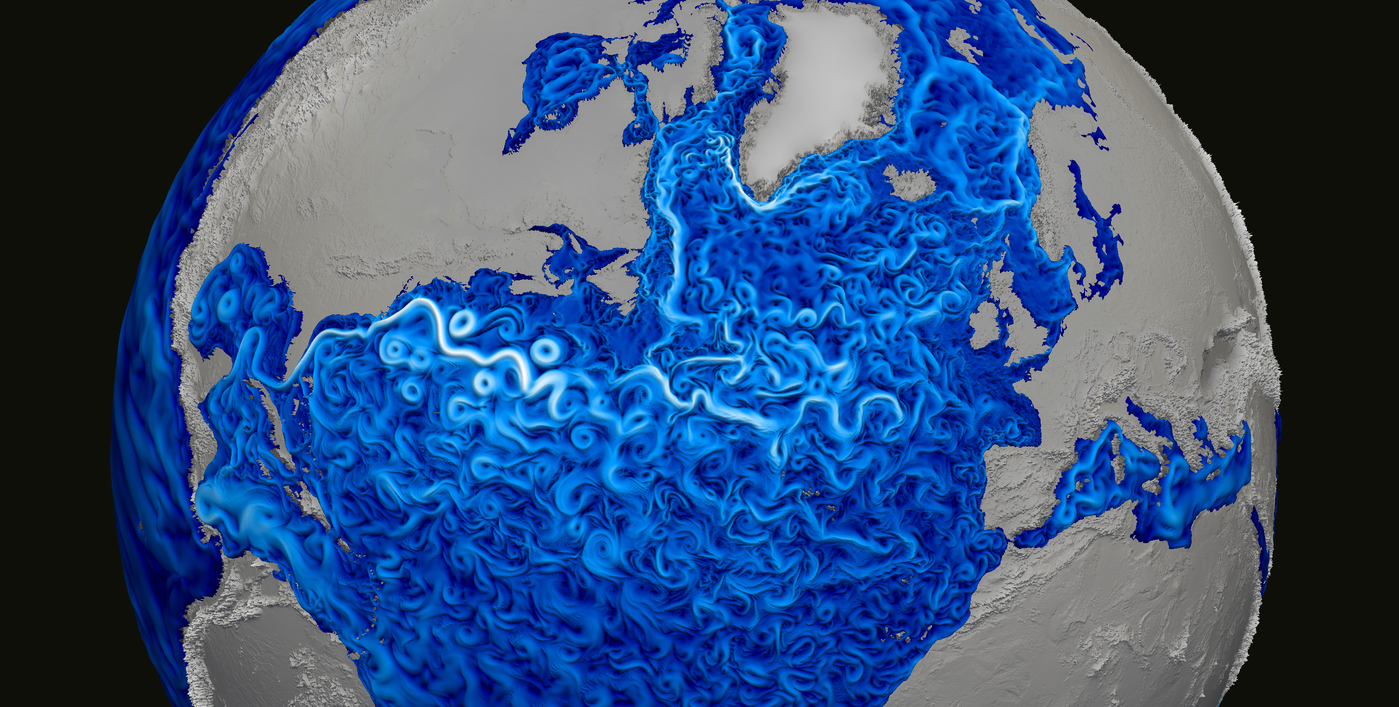
\includegraphics[width=\paperwidth,height=\paperheight,keepaspectratio]{ocean/figures/cover_V3_KE_NA37-7km_cropped_d.png}%
}}}

\newcommand{\inlineCode}[1]{\textbf{#1}}

\newcommand{\core}{seaice}

\begin{document}
%\AddToShipoutPicture*{\BackgroundPic}

\title{
\Huge MPAS-Seaice Model User's Guide \\
\LARGE Version: \version
}

\author{
\LARGE Climate, Ocean, Sea-Ice Modeling Team\\ \\
\LARGE Los Alamos National Laboratory
}

\date{PUT RELEASE DATE HERE May 1, 2018}

\maketitle

\chapter*{Copyright}
\label{chap:copyright}
{\bf Copyright \copyright 2013,  Los Alamos National Security, LLC (LANS) (LA-CC-13-047)
and the University Corporation for Atmospheric Research (UCAR).} \\

All rights reserved.  \\

LANS is the operator of the Los Alamos National Laboratory under Contract No.
DE-AC52-06NA25396 with the U.S. Department of Energy.  UCAR manages the National
Center for Atmospheric Research under Cooperative Agreement ATM-0753581 with the
National Science Foundation.  The U.S. Government has rights to use, reproduce,
and distribute this software.  NO WARRANTY, EXPRESS OR IMPLIED IS OFFERED BY
LANS, UCAR OR THE GOVERNMENT AND NONE OF THEM ASSUME ANY LIABILITY FOR THE USE
OF THIS SOFTWARE.  If software is modified to produce derivative works, such
modified software should be clearly marked, so as not to confuse it with the
version available from LANS and UCAR. \\

Additionally, redistribution and use in source and binary forms, with or without
modification, are permitted provided that the following conditions are met: \\

1) Redistributions of source code must retain the above copyright notice, this
list of conditions and the following disclaimer. \\

2) Redistributions in binary form must reproduce the above copyright notice,
this list of conditions and the following disclaimer in the documentation and/or
other materials provided with the distribution. \\

3) None of the names of LANS, UCAR or the names of its contributors, if any, may
be used to endorse or promote products derived from this software without
specific prior written permission. \\

THIS SOFTWARE IS PROVIDED BY THE COPYRIGHT HOLDERS AND CONTRIBUTORS "AS IS" AND
ANY EXPRESS OR IMPLIED WARRANTIES, INCLUDING, BUT NOT LIMITED TO, THE IMPLIED
WARRANTIES OF MERCHANTABILITY AND FITNESS FOR A PARTICULAR PURPOSE ARE
DISCLAIMED. IN NO EVENT SHALL THE COPYRIGHT HOLDER OR CONTRIBUTORS BE LIABLE FOR
ANY DIRECT, INDIRECT, INCIDENTAL, SPECIAL, EXEMPLARY, OR CONSEQUENTIAL DAMAGES
(INCLUDING, BUT NOT LIMITED TO, PROCUREMENT OF SUBSTITUTE GOODS OR SERVICES;
LOSS OF USE, DATA, OR PROFITS; OR BUSINESS INTERRUPTION) HOWEVER CAUSED AND ON
ANY THEORY OF LIABILITY, WHETHER IN CONTRACT, STRICT LIABILITY, OR TORT
(INCLUDING NEGLIGENCE OR OTHERWISE) ARISING IN ANY WAY OUT OF THE USE OF THIS
SOFTWARE, EVEN IF ADVISED OF THE POSSIBILITY OF SUCH DAMAGE.
\newpage


\tableofcontents

\part{The MPAS Framework}
\chapter{Building MPAS}
\label{chap:mpas_build_instructions}

\section{Prequisites}

To build MPAS, compatible C and Fortran compilers are required. Additionally, the MPAS software relies on the PIO parallel I/O library to read and write model fields, and the PIO library requires the standard netCDF library as well as the parallel-netCDF library from Argonne National Labs. All libraries must be compiled with the same compilers that will be used to build MPAS. Section \ref{sec:build_io} summarizes the basic procedure of installing the required I/O libraries for MPAS.

In order for the MPAS makefiles to find the PIO, parallel-netCDF, and netCDF include files and libraries, the environment variables {\tt PIO}, {\tt PNETCDF}, and {\tt NETCDF} should be set to the root installation directories of the PIO, parallel-netCDF, and netCDF installations, respectively. Newer versions of the netCDF library use a separate Fortran interface library; the top-level MPAS Makefile attempts to add {\tt -lnetcdff} to the linker flags, but some linkers require that {\tt -lnetcdff} appear before {\tt -lnetcdf}, in which case {\tt -lnetcdff} will need to be manually added just before {\tt -lnetcdf} in the specification of {\tt LIBS} in the top-level Makefile.

An MPI installation such as MPICH or OpenMPI is also required, and there is no option to build a serial version of the MPAS executables. There is currently no support for shared-memory parallelism with OpenMP within the MPAS framework.


\section{Compiling I/O Libraries}
\label{sec:build_io}

{\bf NOTE:} It's important to note the MPAS Developers are not responsible for any of the libraries that are used within MPAS. Support for specific libraries should be taken up with the respective developer groups.

Although most recent versions of the I/O libraries should work, the most tested versions of these libraries are: netCDF 4.1.3, parallel-netCDF 1.3.1, and PIO 1.4.1. The netCDF and parallel-netCDF libraries must be installed before building PIO library.

All commands are presented for csh, and will not work if pasted into another shell. Please translate them to the appropraite commands in your shell.

\subsection{netCDF}

Version 4.1.3 of the netCDF library may be downloaded from \url{http://www.unidata.ucar.edu/downloads/netcdf/netcdf-4\_1\_3/index.jsp}.
Assuming the gfortran and gcc compilers will be used, the following shell commands are generally sufficient to install netCDF.

\vspace{12pt}
{\tt > setenv FC gfortran}

{\tt > setenv F77 gfortran} 

{\tt > setenv F90 gfortran}

{\tt > setenv CC gcc} 

{\tt > ./configure --prefix=XXXXX --disable-dap --disable-netcdf-4 --disable-cxx \hfill\break --disable-shared --enable-fortran} 

{\tt > make all check}

{\tt > make install}
\vspace{12pt}

Here, {\tt XXXXX} should be replaced with the directory that will serve as the root installation directory for netCDF.
{\em Before proceeding to compile PIO the {\tt NETCDF\_PATH} environment variable should be set to the netCDF root installation directory.}

Certain compilers require addition flags in the CPPFLAGS environment variable. Please refer to the netCDF installation instructions for these flags.

\subsection{parallel-netCDF}

Version 1.3.1 of the parallel-netCDF library may be downloaded from \url{https://trac.mcs.anl.gov/projects/parallel-netcdf/wiki/Download}.
Assuming the gfortran and gcc compilers will be used, the following shell commands are generally sufficient to install parallel-netCDF.

\vspace{12pt}
{\tt > setenv MPIF90 mpif90}

{\tt > setenv MPIF77 mpif90} 

{\tt > setenv MPICC mpicc}  

{\tt > ./configure --prefix=XXXXX} 

{\tt > make}

{\tt > make install}
\vspace{12pt}

Here, {\tt XXXXX} should be replaced with the directory that will serve as the root installation directory for parallel-netCDF.
{\em Before proceeding to compile PIO the {\tt PNETCDF\_PATH} environment variable should be set to the parallel-netCDF root installation directory.}


\subsection{PIO}

Instructions for building PIO can be found at \url{http://www.cesm.ucar.edu/models/pio/}. Please refer to these instructions for building PIO.

After PIO is built, and installed the PIO enviroment variable needs to be
defined to point at the directory PIO is installed into. Older versions of PIO
cannot be installed, and the PIO environment variable needs to be set to the
directory where PIO was built instead.

\section{Compiling MPAS}

{\bf \em Before compiling MPAS, the {\tt NETCDF}, {\tt PNETCDF}, and {\tt PIO} environment variables must be set to the library installation directories as
described in the previous section. A {\tt CORE} variable also needs to either be defined or passed in during the make process. If {\tt CORE} is not specified, 
the build process will fail.}

The MPAS code uses only the `make' utility for compilation. Rather than employing a separate configuration step
before building the code, all information about compilers, compiler flags, etc., is contained in the top-level {\tt Makefile}; each
supported combination of compilers (i.e., a configuration) is included in the {\tt Makefile} as a separate make target, and the user selects among
these configurations by running {\tt make} with the name of a build target specified on the command-line, e.g.,

\vspace{12pt}
{\tt > make gfortran}
\vspace{12pt}

\noindent to build the code using the GNU Fortran and C compilers. Some of the available targets are listed in the table below, and additional
targets can be added by simply editing the {\tt Makefile} in the top-level directory.

\vspace{12pt}
\begin{longtable}{| l | l | l | l |}
\hline
Target & Fortran compiler & C compiler & MPI wrappers \\ \hline \hline
{\tt xlf} & xlf90 & xlc & mpxlf90 / mpcc \\ \hline
{\tt pgi} & pgf90 & pgcc & mpif90 / mpicc \\ \hline
{\tt ifort} & ifort & gcc & mpif90 / mpicc \\ \hline
{\tt gfortran} & gfortran & gcc & mpif90 / mpicc \\ \hline
{\tt g95} & g95 & gcc & mpif90 / mpicc \\ \hline
\end{longtable}
\vspace{12pt}

In order to get a more complete and up-to-date list of available tagets, one can use the following command within the top-level of MPAS. {\bf NOTE: }This command is known to not work with Mac OSX.
{\small
\begin{verbatim}
> make -rpn | sed -n -e '/^$/ { n ; /^[^ ]*:/p }' | sed "s/: *.*$//g"
\end{verbatim}
}

The MPAS framework supports multiple {\em cores} --- currently a shallow water
model, an ocean model, a non-hydrostatic atmosphere model, and a non-hydrostatic atmosphere initialization core --- so the build
process must be told which core to build. This is done by either setting the environment variable
{\tt CORE} to the name of the model core to build, or by specifying the core to be built explicitly on the command-line
when running {\tt make}. For the shallow water core, for example, one may run either

\vspace{12pt}
{\tt > setenv CORE sw}

{\tt > make gfortran}
\vspace{12pt}

\noindent or

\vspace{12pt}
{\tt > make gfortran CORE=sw}
\vspace{12pt}

If the {\tt CORE} environment variable is set and a core is specified on the command-line, the command-line value takes precedence; if no core
is specified, either on the command line or via the {\tt CORE} environment variable, the build process will stop with an error message stating such.
Assuming compilation is successful, the model executable, named {\tt \$\{CORE\}\_model.exe} (e.g., {\tt sw\_model.exe}), should
be created in the {\tt src/} subdirectory, and a symbolic link to the model executable 
should exist in the top-level MPAS directory.

In order to get a list of available cores, one can simply run the top-level {\tt Makefile} without setting the {\tt CORE} environment variable, or passing the core via the command-line. And example of the output from this can be seen below.

{\small
\begin{verbatim}
> make
( make error )
make[1]: Entering directory `/home/douglasj/Documents/svn-mpas-model.cgd.ucar.edu/trunk/mpas'

Usage: make target CORE=[core] [options]

Example targets:
ifort
gfortran
xlf
pgi

Availabe Cores:
atmosphere
init_atmosphere
ocean
sw

Available Options:
DEBUG=true    - builds debug version. Default is optimized version.
USE_PAPI=true - builds version using PAPI for timers. Default is off.
TAU=true      - builds version using TAU hooks for profiling. Default is off.

Ensure that NETCDF, PNETCDF, PIO, and PAPI (if USE_PAPI=true) are environment variables
that point to the absolute paths for the libraries.

************ ERROR ************
No CORE specified. Quitting.
************ ERROR ************

make[1]: Leaving directory `/home/douglasj/Documents/svn-mpas-model.cgd.ucar.edu/trunk/mpas'
\end{verbatim}
}

\section{Cleaning}

To remove all files  that were created when the model was built, including the model executable itself, {\tt make} may
be run for the `clean' target:

\vspace{12pt}
{\tt > make clean}
\vspace{12pt}

As with compiling, the core to be cleaned is specified by the {\tt CORE} environment variable, or by specifying a core explicitly on the command-line with {\tt CORE=}.


\section{Graph partitioning with METIS} 
\label{sec:metis}

% this section is also in mpas_grid_generation.tex.  When grid generation is included in a future release, delete this section from this chapter.

Before MPAS can be run in parallel, a mesh decomposition file with an appropriate number of 
partitions (equal to the number of MPI tasks that will be used) is required in the run directory.  A limited number of mesh decomposition files ({\tt graph.info.part.*}) are provided with each test case.  In order to create new mesh decomposition files for your desired number of partitions, begin with the provided {\tt graph.info} file and partition with METIS software (\url{http://glaros.dtc.umn.edu/gkhome/views/metis}). The serial graph partitioning program, METIS (rather than ParMETIS or hMETIS) should be sufficient for quickly partitioning any SCVT produced by the grid\_gen mesh generator.

After installing METIS, a {\tt graph.info} file may be partitioned into $N$ partitions by running

\vspace{12pt}
{\tt > gpmetis graph.info} $N$
\vspace{12pt}

\noindent The resulting file, {\tt graph.info.part.}$N$, can then be copied into the MPAS run directory
before running the model with $N$ MPI tasks.

\chapter{Grid Description}
\label{chap:mpas_grid_description}

This chapter provides a brief introduction to the common types of grids used in the MPAS framework. 

The MPAS grid system requires the definition of seven elements. These seven elements are composed of two types of {\it cells}, two types of {\it lines}, and three types of {\it points}. These elements are depicted in Figure \ref{figure:variablePosition} and defined in Table \ref{table:variablePosition}.  These elements can be defined on either the plane or the surface of the sphere. The two types of cells form two meshes, a primal mesh composed of Voronoi regions and a dual mesh composed of Delaunay triangles. Each corner of a primal mesh cell is uniquely associated with the ``center'' of a dual mesh cell and vice versa. So we define the two mesh as either a primal mesh (composed of cells $P_i$) or a dual mesh (composed of cells $D_v$). The center of any primal mesh cell, $P_i$, is denoted by ${\bf x}_i$ and the center of any the dual mesh cell, $D_v$, is denoted by ${\bf x}_v$. The boundary of a given primal mesh cell $P_i$ is composed of the set of lines that connect the ${\bf x}_v$ locations of associated dual mesh cells $D_v$. Similarly, the boundary of a given dual mesh cell $D_v$ is composed of the set of lines that connect the ${\bf x}_i$ locations of the associated primal mesh cells $P_i$. 

As shown in Figure \ref{figure:variablePosition}, a line segment that connects two primal mesh cell centers is uniquely associated with a line segment that connects two dual mesh cell centers. We assume that these two line segments cross and the point of intersection is labeled as ${\bf x}_e$. In addition, we assume that these two line segments are orthogonal as indicated in Figure \ref{figure:variablePosition}. Each ${\bf x}_e$ is associated with two distances: $d_e$ measures the distance between the primal mesh cells sharing ${\bf x}_e$ and $l_e$ measures the distance between the dual mesh cells sharing ${\bf x}_e$.

Since the two line segments crossing at ${\bf x}_e$ are orthogonal, these line segments form a convenient local coordinate system for each edge. At each ${\bf x}_e$ location a unit vector ${\bf n}_e$ is defined to be parallel to the line connecting primal mesh cells. A second unit vector ${\bf t}_e$ is defined such that ${\bf t}_e = {\bf k} \times {\bf n}_e$.

In addition to these seven element types, we require the definition of {\it sets of elements}. In all, eight different types of sets are required and these are defined and explained in Table \ref{table:gridConnectivity} and Figure \ref{figure:gridConnectivity}. The notation is always of the form of, for example, $i \in CE(e)$, where the LHS indicates the type of element to be gathered (cells) based on the RHS relation to another type of element (edges).

Table \ref{table:gridFileName} provides the names of all {\it elements} and all {\it sets of elements} as used in the MPAS framework.  Elements appear twice in the table when described in the grid file in more than one way, e.g. points are described with both cartesian and latitude/longitude coordinates. An ``ncdump -h'' of any MPAS grid, output or restart file will contain all variable names shown in second column of Table  \ref{table:gridFileName}.


\begin{table}[t]
\caption{Definition of elements used to build the MPAS grid.}
\label{table:variablePosition}
\begin{center}
\begin{tabular}{lll}
\hline\hline
$Element$ & $Type$ & $Definition$\\
\hline
 ${\bf x}_i$   & point             & location of center of primal-mesh cells \\
 ${\bf x}_v$  &  point            & location of center of dual-mesh cells \\
 ${\bf x}_e$  & point             & location of edge points where velocity is defined \\
 $d_{e}$       & line segment & distance between neighboring ${\bf x}_i$ locations \\
 $l_{e}$       & line segment & distance between neighboring ${\bf x}_v$ locations \\
 $P_i$         & cell                 & a cell on the primal-mesh \\
 $D_v$        & cell                 & a cell on the dual-mesh \\
\hline
\end{tabular}
\end{center}
\end{table}
%
\begin{table}[t]
\caption{Definition of element groups used to reference connections in the MPAS grid. Examples are provided in Figure \ref{figure:gridConnectivity}.}
\label{table:gridConnectivity}
\begin{center}
\begin{tabular}{lll}
\hline\hline
$Syntax$ & $ouptut$\\
\hline
 $e \in EC(i) $   & set of edges that define the boundary of $P_i$. \\
 $e \in EV(v) $     & set of edges that define the boundary of $D_v$. \\
 $i \in CE(e) $                 & two primal-mesh cells that share edge $e$. \\
 $i \in CV(v) $  &  set of primal-mesh cells that form the vertices of dual mesh cell $D_v$. \\
 $v\in VE(e) $  & the two dual-mesh cells that share edge $e$. \\
 $v \in VI(i) $   & the set of dual-mesh cells that form the vertices of primal-mesh cell $P_i$. \\
 $e \in ECP(e)$ & edges of cell pair meeting at edge $e$. \\
 $e \in EVC(v,i)$ & edge pair associated with vertex $v$ and mesh cell $i$. \\
\hline
\end{tabular}
\end{center}
\end{table}
%

\begin{table}[t]
\caption{Variable names used to describe a MPAS grid.}
\label{table:gridFileName}
\begin{center}
\begin{tabular}{llll}
\hline\hline
$Element$ & $Name$ & $Size$ & $Comment$\\
\hline
 ${\bf x}_i$   & \{x,y,z\}Cell          & nCells  & cartesian location of ${\bf x}_i$  \\
 ${\bf x}_i$   & \{lon,lat\}Cell        & nCells  & longitude and latitude of  ${\bf x}_i$  \\
 ${\bf x}_v$   & \{x,y,z\}Vertex      & nVertices  & cartesian location of ${\bf x}_v$  \\
 ${\bf x}_v$   & \{lon,lat\}Vertex    & nVertices  & longitude and latitude of  ${\bf x}_v$  \\
 ${\bf x}_e$   & \{x,y,z\}Edge          & nEdges  & cartesian location of ${\bf x}_e$  \\
 ${\bf x}_e$   & \{lon,lat\}Edge        & nEdges  & longitude and latitude of  ${\bf x}_e$  \\
 $d_{e}$       & dcEdge                   & nEdges  & distance between ${\bf x}_i$ locations\\
 $l_{e}$         & dvEdge             & nEdges &  distance between ${\bf x}_v$ locations \\
  &  & & \\
 $e \in EC(i) $   &  edgesOnCell  & (nEdgesMax,nCells) & edges that define $P_i$. \\
 $e \in EV(v) $     & edgesOnVertex &  (3,nCells) & edges that define $D_v$. \\
 $i \in CE(e) $      & cellsOnEdge &  (2,nEdges) &  primal-mesh cells that share edge $e$. \\
 $i \in CV(v) $  &   cellsOnVertex &  (3,nVertices) &  primal-mesh cells that define $D_v$. \\
 $v\in VE(e) $  & verticesOnEdge &  (2,nEdges) &    dual-mesh cells that share edge $e$. \\
 $v \in VI(i) $   & verticesOnCell &  (nEdgesMax,nCells) & vertices that define $P_i$. \\
\hline
\end{tabular}
\end{center}
\end{table}
%


%
\begin{figure}[t]
  \noindent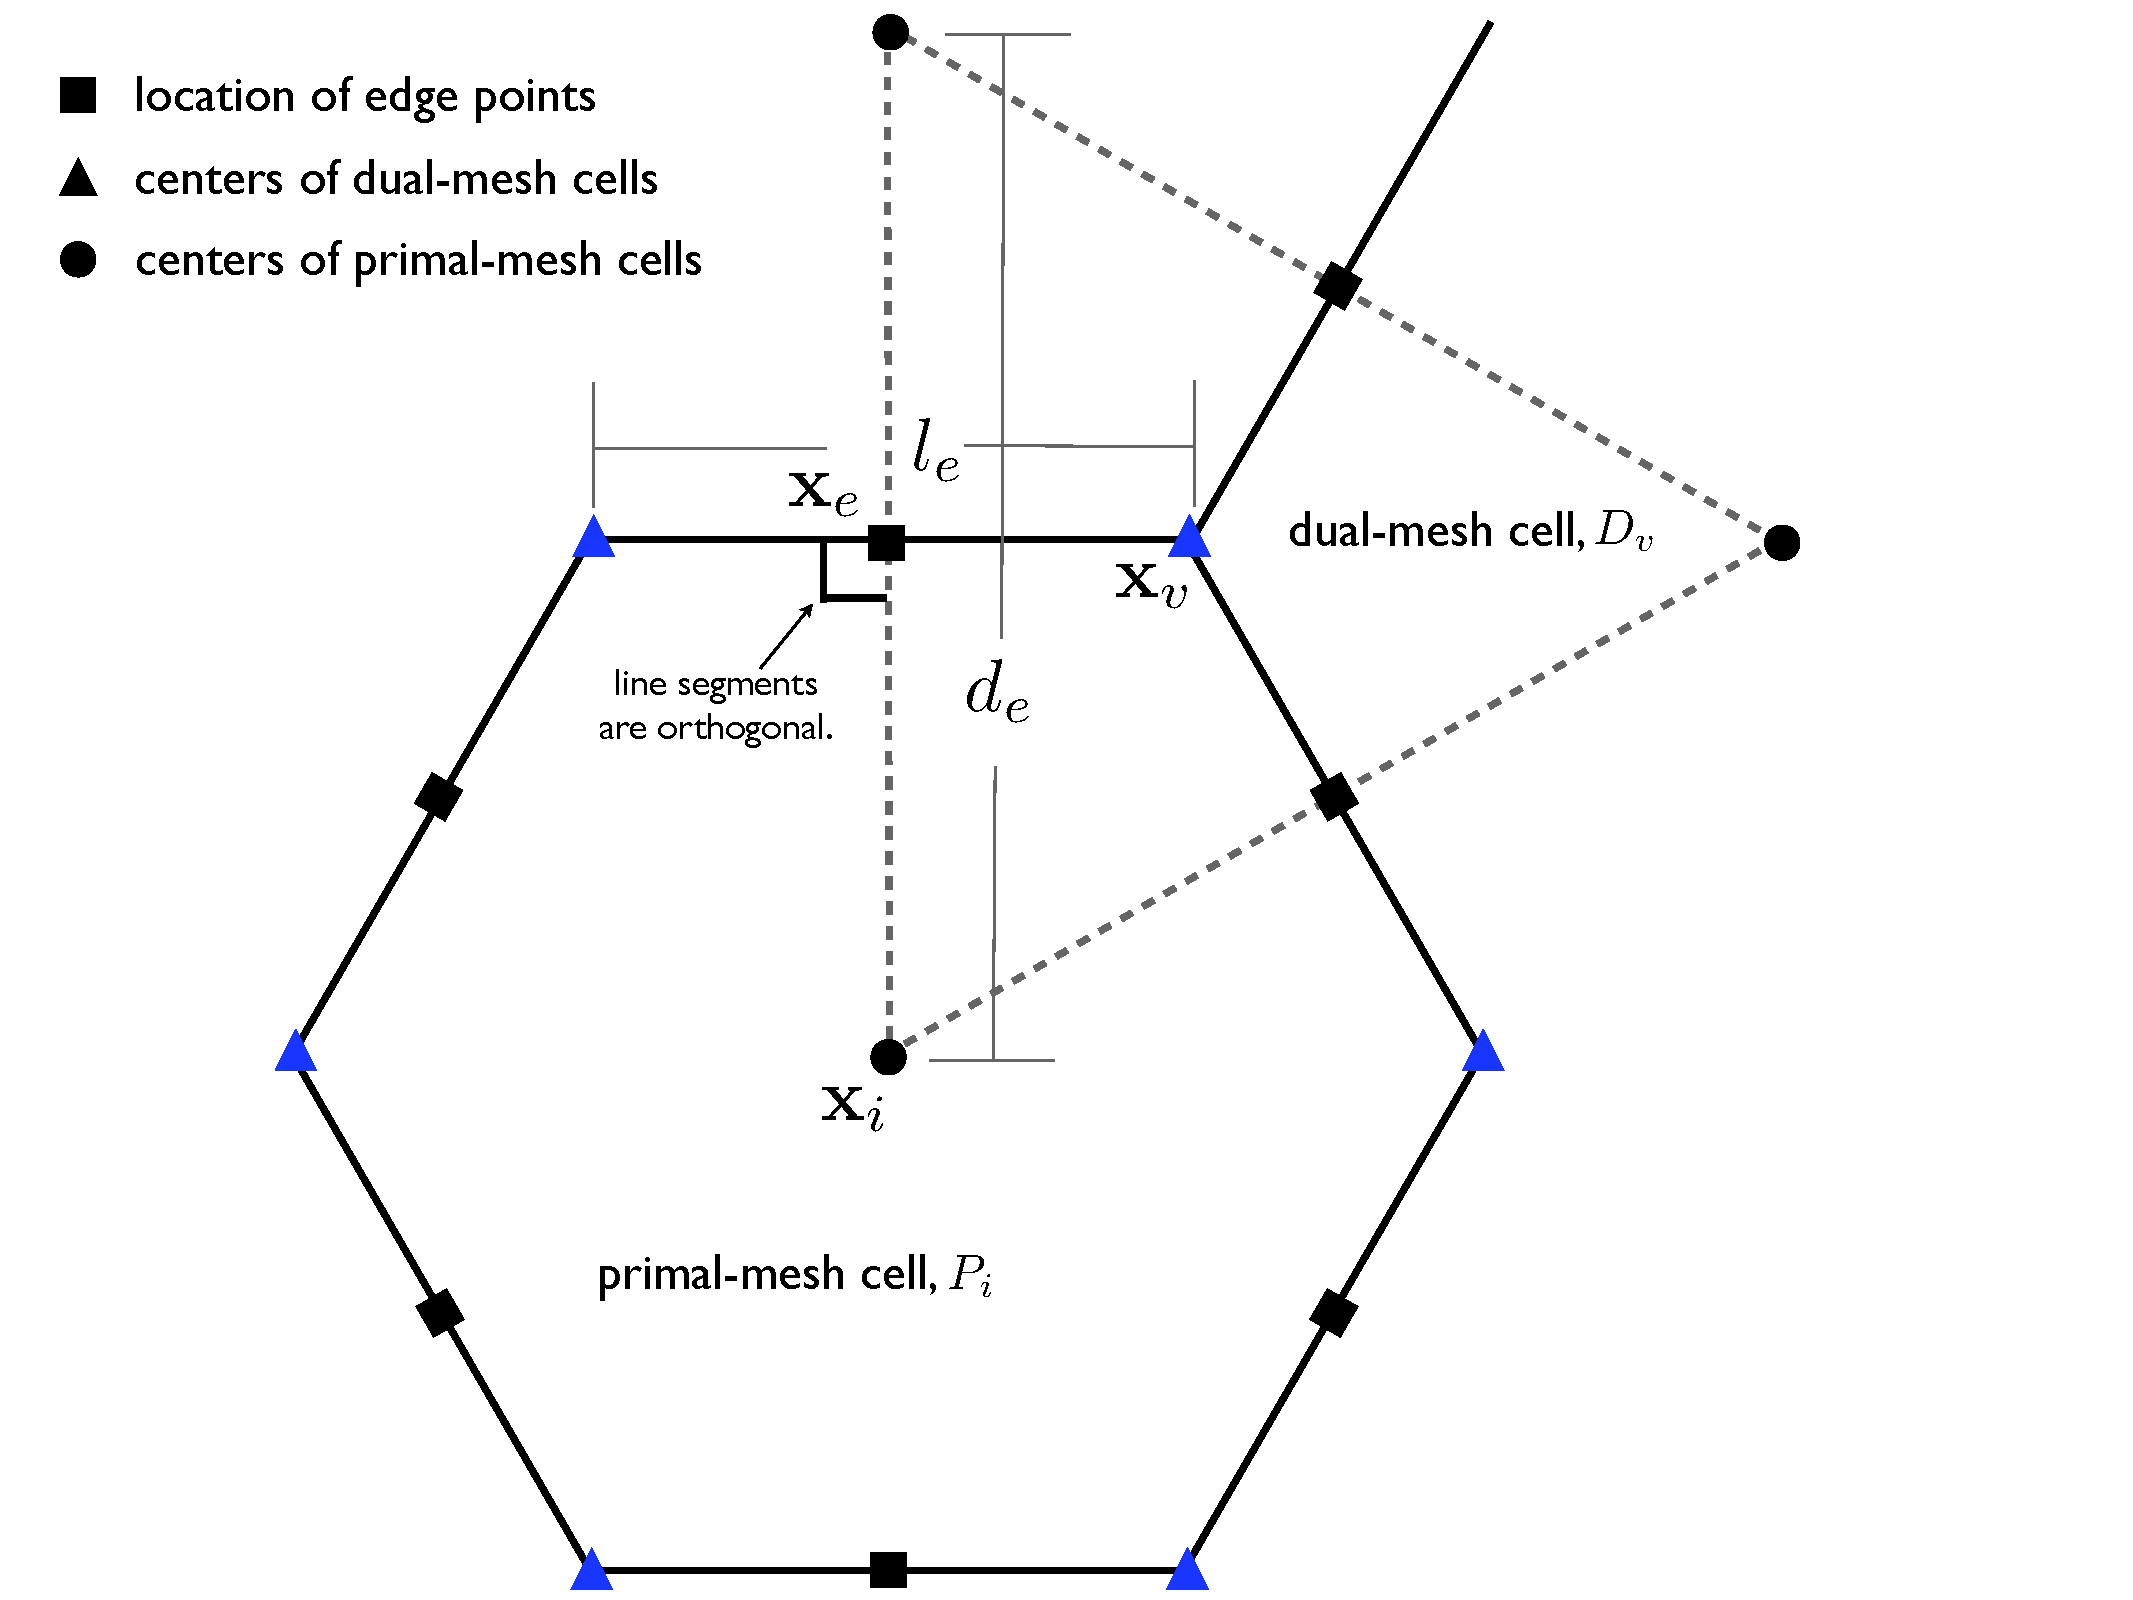
\includegraphics[width=16cm,angle=0]{./shared/figures/variablePosition.pdf}\\
  \caption{Definition of elements used to build the MPAS grid. Also see Table \ref{table:variablePosition}.}
  \label{figure:variablePosition}
\end{figure}

%
\begin{figure}[t]
   \noindent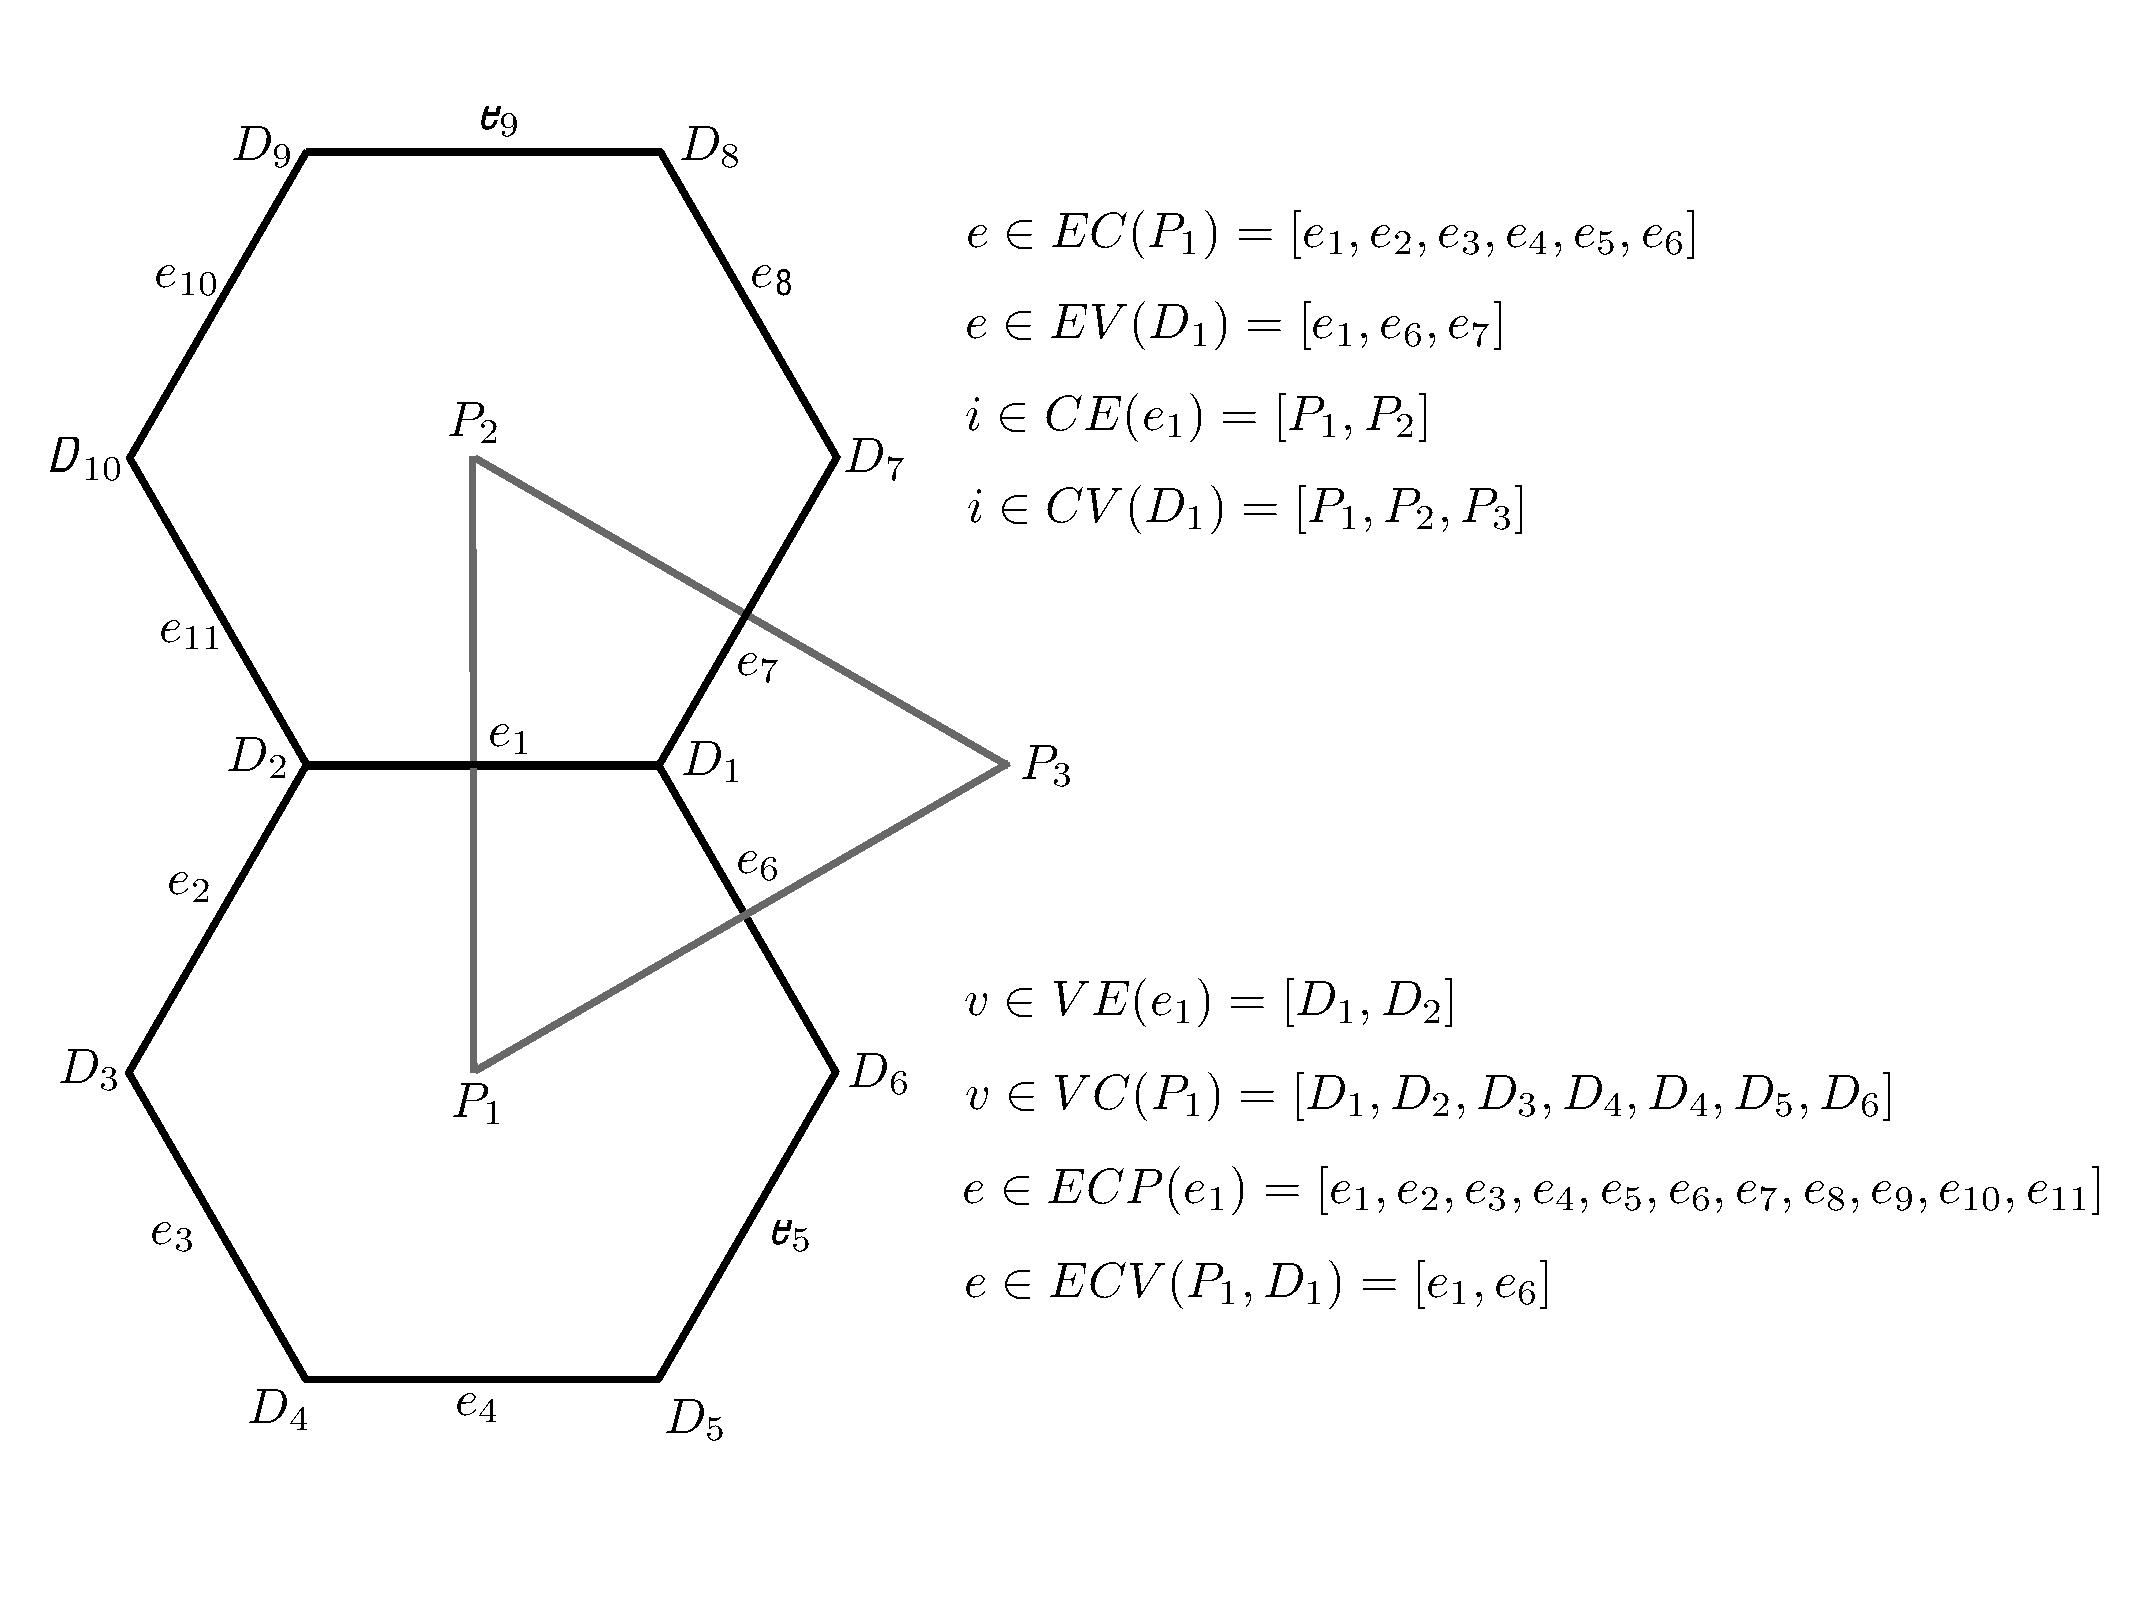
\includegraphics[width=16cm,angle=0]{./shared/figures/gridConnectivity.pdf}\\
  \caption{Definition of element groups used to reference connections in the MPAS grid. Also see Table \ref{table:gridConnectivity}.}
  \label{figure:gridConnectivity}
\end{figure}



\chapter{Configuring Model Input and Output}
\label{chap:mpas_io}

\newlength{\immindent}
\settowidth{\immindent}{{\tt <immutable\_stream }}


\newlength{\mutindent}
\settowidth{\mutindent}{{\tt <stream }}

The reading and writing of model fields in MPAS is handled by user-configurable {\em streams}. 
A stream represents a fixed set of model fields, together with dimensions and attributes, that are
all written or read together to or from the same file or set of files. Each MPAS model core may define
its own set of default streams that it typically uses for reading initial conditions, for writing and reading
restart fields, and for writing additional model history fields. Besides these default streams, users may define
new streams to, e.g., write certain diagnostic fields at a higher temporal frequency than the usual model
history fields.

Streams are defined in XML configuration files that are created at build time for each model core. The name
of this XML file is simply `streams.' suffixed with the name of the core. For example, the streams for
the {\em sw} (shallow-water) core are defined in a file named `streams.sw'. An XML stream
file may further reference other text files that contain lists of the model fields that are read or written in
each of the streams defined in the XML stream file.

Changes to the XML stream configuration file will take effect the next time an MPAS core is run; there is no need
to re-compile after making modifications to the XML files. As described in the next section, it is therefore possible, e.g.,
to change the interval at which a stream is written, the template for the filenames associated with a stream, or the 
set of fields that are written to a stream, without the need to re-compile any code.

Two classes of streams exist in MPAS: {\em immutable} streams and {\em mutable} streams. Immutable streams
are those for which the set of fields that belong to the stream may not be modified at model run-time; however, it is
possible to modify the interval at which the stream is read or written, the filename template describing the files
containing the stream on disk, and several other parameters of the stream. In contrast, all aspects of mutable streams,
including the set of fields that belong to the stream, may be modified at run-time. The motivation for the creation of
two stream classes is the idea that an MPAS core may not function correctly if certain fields are not read in upon 
model start-up or written to restart files, and it is therefore not reasonable for users to modify this set of required fields 
at run-time. An MPAS core developer may choose to implement such streams as immutable streams. Since fields may
not be added to an immutable stream at run-time, new immutable streams may not be defined at run-time, and the only 
type of new stream that may be defined at run-time is the mutable stream type.

\section{XML stream configuration files}
\label{sec:xml_stream_format} 

The XML stream configuration file for an MPAS core always has a parent XML {\em element} named {\tt streams}, within which 
individual streams are defined:

\vspace{12pt}
\noindent {\tt <streams>} \newline
\newline
\hspace*{1cm}... one or more stream definitions ... \newline
\newline
\noindent {\tt </streams>} \newline
\vspace{12pt}

Immutable streams are defined with the {\tt immutable\_stream} element, and mutable streams are defined with the {\tt stream}
element: 

\vspace{12pt}
\noindent {\tt <immutable\_stream name="initial\_conditions"} \newline
\hspace*{\immindent}{\tt type="input"} \newline
\hspace*{\immindent}{\tt filename\_template="init.nc"} \newline
\hspace*{\immindent}{\tt input\_interval="initial\_only"} \newline
\hspace*{\immindent}{\tt />} \newline
\vspace{12pt} \newline
\noindent {\tt <stream name="history"} \newline
\hspace*{\mutindent}{\tt type="output"} \newline
\hspace*{\mutindent}{\tt filename\_template="output.\$Y-\$M-\$D\_\$h.\$m.\$s.nc"} \newline
\hspace*{\mutindent}{\tt output\_interval="6:00:00" >} \newline
\newline
\hspace*{1cm}... model fields belonging to this stream ... \newline
\newline
\noindent {\tt </stream>} \newline
\vspace{12pt}

As shown in the example stream definitions, above, both classes of stream have the following required attributes:

\begin{itemize}
\item {\tt name} --- A unique name used to refer to the stream.
\item {\tt type} --- The type of stream, either {\tt "input"}, {\tt "output"}, {\tt "input;output"}, or {\tt "none"}. A stream may be both an input
and an output stream (i.e., {\tt "input;output"}) if, for example, it is read once at model start-up to provide initial conditions and thereafter written 
periodically to provide model checkpoints. A stream may be defined as neither input nor output (i.e., {\tt "none"}) for the purposes of defining a 
set of fields for inclusion other streams. Note that, for immutable streams, the type attribute may not be changed at run-time.
\item {\tt filename\_template} --- The template for files that exist or will be created by the stream. The filename template may include any of the
following variables, which are expanded based on the simulated time at which files are first created.
\begin{itemize}
\item {\tt \$Y} --- Year
\item {\tt \$M} --- Month
\item {\tt \$D} --- Day of the month
\item {\tt \$d} --- Day of the year
\item {\tt \$h} --- Hour
\item {\tt \$m} --- Minute
\item {\tt \$s} --- Second
\end{itemize}
A filename template may include either a relative or an absolute path, in which case MPAS will attempt to create any directories 
in the path that do not exist, subject to filesystem permissions.
\item {\tt input\_interval} --- For streams that have type {\tt "input"} or {\tt "input;output"}, the interval, beginning at the model initial time,
at which the stream will be read. Possible values include a time interval specification in the format {\tt "YYYY-MM-DD\_hh:mm:ss"}; the value 
{\tt "initial\_only"}, which specifies that the stream is read only once at the model initial time; or the value {\tt "none"}, which specifies that 
the stream is not read during a model run.
\item {\tt output\_interval} --- For streams that have type {\tt "output"} or {\tt "input;output"}, the interval, beginning at the model initial time,
at which the stream will be written. Possible values include a time interval specification in the format {\tt "YYYY-MM-DD\_hh:mm:ss"}; the value 
{\tt "initial\_only"}, which specifies that the stream is written only once at the model initial time; or the value {\tt "none"}, which specifies that 
the stream is not written during a model run.
\end{itemize}

Finally, the set of fields that belong to a mutable stream may be specified with any combination of the following elements. Note that, for 
immutable streams, no fields are specified at run-time in the XML configuration file.

\begin{itemize}
\item {\tt var} --- Associates the specified variable with the stream. The variable may be any of those defined in an MPAS core's Registry.xml file, but may
not include individual constituent arrays from a var\_array.
\item {\tt var\_array} --- Associates all constituent variables in a var\_array, defined in an MPAS core's Registry.xml file, with the stream.
\item {\tt var\_struct} --- Associates all variables in a var\_struct, defined in an MPAS core's Registry.xml file, with the stream.
\item {\tt stream} --- Associates all explicitly associated fields in the specified stream with the stream; streams are not recursively included.
\item {\tt file} --- Associates all variables listed in the specified text file, with one field per line, with the stream.
\end{itemize}

\section{Optional stream attributes}
\label{sec:optional_stream_atts} 

Besides the required attributes described in the preceding section, several additional, optional attributes may be added to
the definition of a stream.

\begin{itemize}
\item {\tt filename\_interval} --- The interval between the timestamps used in the construction of the names of files associated with
a stream. Possible values include a time interval specification in the format {\tt "YYYY-MM-DD\_hh:mm:ss"}; the value {\tt "none"}, indicating
that only one file containing all times is associated with the stream; the value {\tt "input\_interval"} that, for input type streams, indicates that
each time to be read from the stream will come from a unique file; or the value {\tt "output\_interval"} that, for output type streams, indicates 
that each time to be written to the stream will go to a unique file whose name is based on the timestamp of the data being written. The default
value is {\tt "input\_interval"} for input type streams and {\tt "output\_interval"} for output type streams. For streams of type {\tt "input;output"}, the
default filename interval is {\tt "input\_interval"} if the input interval is an interval (i.e., not {\tt "initial\_only"}), or {\tt "output\_interval"} otherwise. 
Refer to Section \ref{sec:filename_interval_example}
for an example of the use of the filename\_interval attribute.
\item {\tt reference\_time} --- A time that is an integral number of filename intervals from the timestamp of any file associated with the stream.
The default value is the start time of the model simulation. Refer to Section \ref{sec:reference_time_example} for an example of 
the use of the reference\_time attribute.
\item {\tt clobber\_mode} --- Specifies how a stream should handle attempts to write to a file that already exists. Possible values
for the mode include:
\begin{itemize}
\item {\tt "overwrite"} --- The stream is allowed to overwrite records in existing files and to append new records 
to existing files; records not explicitly written to are left untouched.
\item {\tt "truncate"} or {\tt "replace\_files"} --- The stream is allowed to overwrite existing files, which are first truncated 
to remove any existing records; this is equivalent to replacing any existing files with newly created files of the same name.
\item {\tt "append"} --- The stream is only allowed to append new records to existing files; existing records may not be overwritten.
\item {\tt "never\_modify"} --- The stream is not allowed to modify existing files in any way.
\end{itemize}
The default clobber mode for streams is {\tt "never\_modify"}. Refer to Section \ref{sec:append_example} for an example of the use of
the clobber\_mode attribute.
\item {\tt precision} --- The precision with which real-valued fields will be written or read in a stream. Possible values include 
{\tt "single"} for 4-byte real values, {\tt "double"} for 8-byte real values, or {\tt "native"}, which specifies that real-valued fields
will be written or read in whatever precision the MPAS core was compiled. The default value is {\tt "native"}. Refer to Section \ref{sec:filename_interval_example}
for an example of the use of the precision attribute.
\item {\tt packages} --- A list of packages attached to the stream. A stream will be active (i.e., read or written) only if at least one of 
the packages attached to it is active, or if no packages at all are attached. Package names are provided as a semi-colon-separated
list. Note that packages may only be defined in an MPAS core's Registry.xml file at build time. By default, no packages are attached
to a stream.
\item {\tt io\_type} --- The underlying library and file format that will be used to read or write a stream. Possible values include:
\begin{itemize}
\item{\tt "pnetcdf"} --- Read/write the stream with classic large-file NetCDF files (CDF-2) using the ANL Parallel-NetCDF library.
\item{\tt "pnetcdf,cdf5"} --- Read/write the stream with large-variable files (CDF-5) using the ANL Parallel-NetCDF library. 
\item{\tt "netcdf"} --- Read/write the stream with classic large-file NetCDF files (CDF-2) using the Unidata serial NetCDF library.
\item{\tt "netcdf4"} --- Read/write the stream with HDF-5 files using the Unidata parallel NetCDF-4 library.
\end{itemize}
Note that the PIO library must have been built with support for the selected {\tt io\_type}. By default, all input and output streams are
read and written using the {\tt "pnetcdf"} option.
\end{itemize}

\section{Stream definition examples}
\label{sec:stream_example} 

This section provides several example streams that make use of the optional stream attributes described in Section \ref{sec:optional_stream_atts}.
All examples are of output streams, since it is more likely that a user will need to write additional fields than to read additional fields, which a model would need to be aware of; however, the concepts that are illustrated here translate directly to input streams as well.

\subsection{Example: a single-precision output stream with one month of data per file}
\label{sec:filename_interval_example}

In this example, the optional attribute specification {\tt filename\_interval="01-00\_00:00:00"} is added to force a new
output file to be created for the stream every month. Note that the general format for time interval specifications is {\tt YYYY-MM-DD\_hh:mm:ss},
where any leading terms can be omitted; in this case, the year part of the interval is omitted. To reduce the file size, the specification
{\tt precision="single"} is also added to force real-valued fields to be written as 4-byte floating-point values, rather than the default of 8 bytes.

\vspace{12pt}
\noindent {\tt <stream name="diagnostics"} \newline
\hspace*{\mutindent}{\tt type="output"} \newline
\hspace*{\mutindent}{\tt filename\_template="diagnostics.\$Y-\$M.nc"} \newline
\hspace*{\mutindent}{\tt filename\_interval="01-00\_00:00:00"} \newline
\hspace*{\mutindent}{\tt precision="single"} \newline
\hspace*{\mutindent}{\tt output\_interval="6:00:00" >} \newline
\newline
\hspace*{1cm}{\tt <var name="u10"/>} \newline
\hspace*{1cm}{\tt <var name="v10"/>} \newline
\hspace*{1cm}{\tt <var name="t2"/>} \newline
\hspace*{1cm}{\tt <var name="q2"/>} \newline
\newline
\noindent {\tt </stream>} \newline
\vspace{12pt}

The only fields that will be written to this stream are the hypothetical 10-m diagnosed wind components, the 2-m temperature, 
and the 2-m specific humidity variables. Also, note that the filename template only includes the year and month from the model 
valid time; this can be problematic when the simulation starts in the middle of a month, and a solution for this problem 
is illustrated in the example of Section \ref{sec:reference_time_example}.

\subsection{Example: appending records to existing output files}
\label{sec:append_example}

By default, streams will never modify existing files whose filenames match the name of a file that would otherwise be written
during the course of a simulation. However, when restarting a simulation that is expected to add more records to existing output 
files, it can be useful to instruct the MPAS I/O system to append these records, thereby modifying existing files. This may be 
accomplished with the {\tt clobber\_mode} attribute.

\vspace{12pt}
\noindent {\tt <stream name="diagnostics"} \newline
\hspace*{\mutindent}{\tt type="output"} \newline
\hspace*{\mutindent}{\tt filename\_template="diagnostics.\$Y-\$M.nc"} \newline
\hspace*{\mutindent}{\tt filename\_interval="01-00\_00:00:00"} \newline
\hspace*{\mutindent}{\tt precision="single"} \newline
\hspace*{\mutindent}{\tt clobber\_mode="append"} \newline
\hspace*{\mutindent}{\tt output\_interval="6:00:00" >} \newline
\newline
\hspace*{1cm}{\tt <var name="u10"/>} \newline
\hspace*{1cm}{\tt <var name="v10"/>} \newline
\hspace*{1cm}{\tt <var name="t2"/>} \newline
\hspace*{1cm}{\tt <var name="q2"/>} \newline
\newline
\noindent {\tt </stream>} \newline
\vspace{12pt}

In general, if MPAS were to attempt to write a record at a time that already existed in an output file, a clobber\_mode 
of `append' would not permit the write to take place, since this would modify existing data; in `append' mode, only new
records may be added. However, due to a peculiarity in the implementation of the `append' clobber mode, it may be 
possible for an output file to contain duplicate times. This can happen when the first record that is appended to 
an existing file has a timestamp not matching any in the file, after which, any record that is written --- regardless of 
whether its timestamp matches one already in the file --- will be appended to the end of the file. This situation may arise, 
for example, when restarting a model simulation with a shorter {\tt output\_interval} than was used in the original model simulation 
with an MPAS core that does not write the first output time for restart runs.

\subsection{Example: referencing filename intervals to a time other than the start time}
\label{sec:reference_time_example}

The example stream of the previous sections creates a new file each month during the simulation, and the filenames
contain only the year and month of the timestamp when the file was created. If a simulation begins at 00 UTC on the
first day of a month, then each file in the diagnostic stream will contain only output times that fall within the month
in the filename. However, if a simulation were to begin in the middle of a month --- for example, the month of June, 2014 --- 
the first diagnostics output file would have a filename of `diagnostics.2014-06.nc', but rather than containing only output
fields valid in June, it would contain all fields written between the middle of June and the middle of July, at which point
one month of simulation would have elapsed, and a new output file, `diagnostics.2014-07.nc', would be created.

In order to ensure that the file `diagnostics.2014-06.nc' contained only data from June 2014, the {\tt reference\_time}
attribute may be added such that the day, hour, minute, and second in the date and time represent the first day of the month
at 00 UTC. In this example, the year and month of the reference time are not important, since the purpose of the reference time
here is to describe to MPAS that the monthly filename interval begins (i.e., is referenced to) the first day of the month.

\vspace{12pt}
\noindent {\tt <stream name="diagnostics"} \newline
\hspace*{\mutindent}{\tt type="output"} \newline
\hspace*{\mutindent}{\tt filename\_template="diagnostics.\$Y-\$M.nc"} \newline
\hspace*{\mutindent}{\tt filename\_interval="01-00\_00:00:00"} \newline
\hspace*{\mutindent}{\tt reference\_time="2014-01-01\_00:00:00"} \newline
\hspace*{\mutindent}{\tt precision="single"} \newline
\hspace*{\mutindent}{\tt clobber\_mode="append"} \newline
\hspace*{\mutindent}{\tt output\_interval="6:00:00" >} \newline
\newline
\hspace*{1cm}{\tt <var name="u10"/>} \newline
\hspace*{1cm}{\tt <var name="v10"/>} \newline
\hspace*{1cm}{\tt <var name="t2"/>} \newline
\hspace*{1cm}{\tt <var name="q2"/>} \newline
\newline
\noindent {\tt </stream>} \newline
\vspace{12pt}

In general, the components of a timestamp, {\tt YYYY-MM-DD\_hh:mm:ss}, that are less significant than (i.e., to the right of) 
those contained in a filename template are important in a reference\_time. For example, with a {\tt filename\_template} that contained
only the year, the month component of the {\tt reference\_time} would become important to identify the month of the year on which
the yearly basis for filenames would begin.



% Grid generation is not included in MPAS release 1.0:
%\appendix{Generating meshes}
\label{chap:mpas_grid_generation}

This chapter describes the steps used to create the  spherical centroidal Voronoi tessellation (SCVT) meshes and mesh-decomposition files used by MPAS models.
Since it can take considerable time (often several days or more) to generate a mesh as described in \S \ref{sec:global_scvt}, it is recommended to obtain 
and use existing SCVT meshes from \url{http://www.mmm.ucar.edu/people/duda/mpas/} whenever possible; these meshes can be quickly
modified to shift or rotate the refinement regions over the geographic areas of interest using the utility program described in \S \ref{sec:grid_rotate}.

\section{Density functions}

In all MPAS models, the horizontal meshes are SCVTs with a C-grid staggering of
velocities. As their name suggests, SCVTs are Voronoi tessellations defined on the surface of a sphere, and in which the generating 
point for each Voronoi region is also the mass centroid of that region with respect to some {\em density function}. An overview of
the application of SCVTs to multi-resolution climate modeling is given in Ringler et al. (2008)
\footnote{Ringler, T., L. Ju and M. Gunzburger, 2008, A multiresolution method for climate system modeling: application of spherical centroidal Voronoi tessellations, {\em Ocean Dynamics}, 58 (5-6), 475-498. doi:10.1007/s10236-008-0157-2.}.

For the purposes of generating SCVTs, the central concern lies with the density function, $\rho$, which is a user-defined
function relating the relative resolutions in different regions of the mesh. Specifically, for two generating points of the 
SCVT, ${\bf x}_i$ and ${\bf x}_j$,
\[
{h_i \over h_j} \approx \left({\rho({\bf x}_j) \over \rho({\bf x}_i)} \right)^{1 \over 4},
\]
where $h_i$ and $h_j$ are the diameters of the Voronoi cells associated with ${\bf x}_i$ and ${\bf x}_j$, respectively.

In the mesh generation program global\_scvt, described in the next section, the density function is defined programatically in the Fortran function
{\tt density\_for\_point()}, which returns the value of the density function, $\rho({\bf x})$, given a location on the sphere, ${\bf x}$.
   
\section{The global\_scvt program}
\label{sec:global_scvt}

\subsection{Compilation}
                                                                                             
As a first step toward building the global\_scvt code, the environment variable                     
{\tt NETCDF} must be set to the root of the netCDF installation. Unlike with the MPAS model, separate make targets are not
defined for each compiler set, and it will generally be necessary to edit the top-level Makefile to set the compiler and compiler flags                 
that will be used to build global\_scvt; however, there are commented-out sections in the Makefile for using either of the ifort, pgf90, or gfortran compilers that may be uncommented or used as a starting point for other compilers. Also, if the netCDF installation has a separate Fortran interface library, {\tt -lnetcdff} will need to be added before {\tt -lnetcdf} in the Makefile. The global\_scvt program is parallelized with OpenMP, so if compiler support is available, OpenMP compiler flags may be added
in the Makefile as well.                      

Before compiling the global\_scvt program, a density function should first be defined in the function {\tt density\_for\_point()} in {\tt src/module\_scvt.F}. The default density function is a uniform density function that returns a value of 1.0 for all locations
on the sphere, and commented code in {\tt density\_for\_point()} may be uncommented to achieve an area of circular refinement. {\em Note that, although $\rho({\bf x})$ could in principle take on any non-negative value, the code to scale eddy viscosities by the mesh resolution in the MPAS model assumes that $\rho({\bf x}) \in (0,1]$, so care should be taken when designing a new density function: a value of 1.0 should correspond to the highest-resolution regions(s) in the mesh.}                                      
                                                                                                
After editing the Makefile and defining the desired density function, running `make' should create the grid\_gen executable 
in the top-level directory. A second program, grid\_ref, may also be created, but this program is not needed by the current version 
of the global\_scvt program.

\subsection{Running}

As will be described in Section \ref{sec:grid_gen_efficiency}, a typical mesh is generated using multiple refinement steps. Within each of these steps, an SCVT with a fixed
number of generating points is converged before the SCVT is refined, giving a larger number of generating points to begin the next step. In this section, the process of converging an SCVT within a single step is described.

Two files are needed in order to run the grid\_gen program: an initial generating point file, {\tt locs.dat}, and a                        
namelist file, {\tt namelist.input}. The {\tt locs.dat} file contains a list of the Cartesian coordinates (assuming a unit-radius sphere
centered at the origin) of each of the beginning generating points, and the {\tt namelist.input} file specifies the number of generating points to be read from the {\tt locs.dat} file, the number of iterations to run, and the convergence criteria; a complete list of namelist variables is provided in the table below.

\vspace{12pt}
\begin{longtable}{|p{1.25in} |p{4.5in}|}
\hline
np & the number of points to read from the {\tt locs.dat} file \\ \hline
locs\_as\_xyz & whether the initial generating points in {\tt locs.dat} are given in Cartesian space ({\tt .true.}) or latitude-longitude space ({\tt .false.}) \\ \hline
n\_scvt\_iterations & the maximum number of Lloyd iterations to perform \\ \hline
eps & the convergence criterion, specifying the maximum permissible average movement of a generating point during an iteration \\ \hline
l2\_conv & whether to stop iterating if the convergence criterion is met \\ \hline
inf\_conv & currently the same meaning as l2\_conv \\ \hline
min\_dx & the targeted minimum grid distance in the mesh, on which an estimate for the number of generating points will be based; see Section \ref{sec:estimating_np} \\ \hline
\end{longtable}
\vspace{12pt}

\noindent A convergence criterion of $1\times10^{-10}$ should be sufficient, and in                     
practice, many thousands of iterations are needed to reach this tolerance.

If grid\_gen was compiled with OpenMP support, the environment variable {\tt OMP\_NUM\_THREADS} can be set to the 
number of threads that will be used by the program. Then, grid\_gen can be run with no command-line arguments:

\vspace{12pt}
{\tt > ./grid\_gen}
\vspace{12pt}
                                                                                         
                                                                                                
When grid\_gen finishes --- either because the convergence criterion has been met, or the
maximum number of iterations have been performed ---  several output files should be created: 

\begin{itemize}
\item {\tt scvt\_initial.ps} --- a plot of the mesh at the start of iterations,
\item {\tt scvt\_final.ps} --- a plot of the mesh after iterations,
\item {\tt grid.nc} --- the actual MPAS mesh file, which can be used with the initialization core to create an MPAS input file,
\item {\tt graph.info} --- information describing the cell connectivity graph of the mesh, to be used with a graph partitioner as described in Section \ref{sec:metis}, and
\item {\tt locs.dat.out} --- a list of the final generating points appended with a set of $3 np - 6$ refinement points. 
\end{itemize}

If the tolerance specified in the {\tt namelist.input} file was met, the SCVT mesh should be sufficiently converged, and the resulting {\tt grid.nc}
file can be used with the initialization program to create an initial condition file for MPAS; alternatively, the full set of $4 np - 6$ refinement points in 
the {\tt locs.dat.out} file can be used as input to the grid\_gen program to create another SCVT with approximately twice the resolution. If, however, the specified tolerance was not met, the {\tt locs.dat.out} file may be copied to {\tt locs.dat}, and further iteration may be performed on the SCVT.

To create a plot of the mesh with coastlines, which can be helpful when locating or sizing refinement regions, the {\tt mesh.ncl} script may be used to plot the mesh directly from                 
the {\tt grid.nc} file.                                                                          

\subsection{Estimating the required number of generating points}
\label{sec:estimating_np}

Setting the {\tt min\_dx} variable in the {\tt namelist.input} file to the targeted minimum grid distance in the mesh and running the grid\_gen program will cause the program to print out an estimate for the number of generating points that will be required to achieve that minimum grid distance with the density function provided in {\tt density\_for\_point()}.

\subsection{Efficiency concerns}
\label{sec:grid_gen_efficiency}

Although one could, given an estimate for the number of generating points needed to achieve the required absolute resolutions in the mesh,
create a {\tt locs.dat} file with that number of randomly chosen points on the unit sphere, and, using that {\tt locs.dat} file, converge a final SCVT, 
experience indicates that a stepwise approach can significantly reduce the required wallclock time.                   

   
\section{The grid\_rotate program} 
\label{sec:grid_rotate} 

The purpose of the grid\_rotate program is simply to rotate an MPAS mesh file, moving a refinement region from one geographic location to another, so that the mesh can be re-used for different applications. This utility was developed out of the need to save computational resources, since generating an SCVT --- particularly one with a large number of generating points or a high degree of refinement --- can take considerable time.

To build the grid\_rotate program, the Makefile should first be edited to set the Fortran compiler to be used; if the netCDF installation pointed to by the {\tt NETCDF} environment variable was build with a separate Fortran interface library, it will also be necessary to add {\tt -lnetcdff} just before {\tt -lnetcdf} in the Makefile. After editing the Makefile, running `make' should result in a grid\_rotate executable file.

Besides the MPAS grid file to be rotated, grid\_rotate requires a namelist file, {\tt namelist.input}, which specifies the rotation to be applied to the mesh. The namelist variables are summarized in the table below
   
\vspace{12pt}
\begin{longtable}{|p{3.25in} |p{2.5in}|}
\hline
config\_original\_latitude\_degrees & original latitude of any point on the sphere \\ \hline
config\_original\_longitude\_degrees & original longitude of any point on the sphere \\ \hline
config\_new\_latitude\_degrees &  latitude to which the original point should be shifted \\ \hline
config\_new\_longitude\_degrees &  longitude to which the original point should be shifted \\ \hline
config\_birdseye\_rotation\_counter\_clockwise\_degrees & rotation about a vector from the sphere center through the original point \\ \hline
\end{longtable}
\vspace{12pt}

\noindent Essentially, one chooses any point on the sphere, decides where that point should be shifted to,
and specifies any change to the orientation (i.e., rotation) of the mesh about that point. 

Having set the rotation parameters in the {\tt namelist.input} file, the grid\_rotate program should be run with two command-line options
specifying the original grid file name and the name of the rotated grid file to be produced, e.g.,

\vspace{12pt}
{\tt > grid\_rotate grid.nc grid\_SE\_Asia\_refinement.nc}
\vspace{12pt}

The original grid file will not be altered, and a new, rotated grid file will be created. The NCL script {\tt mesh.ncl} may be used to plot either of the original or rotated grid files after suitable setting the name of the grid file in the script.
   
   
\section{Graph partitioning with METIS} 
\label{sec:metis}

{\color{red} THIS SECTION WAS COPIED TO mpas_build_instructions.tex  FOR RELEASE 1.0. WHEN GRID GENERATION IS INCLUDED, DELETE THE METIS SECTION FROM mpas_build_instructions.tex}.

Before MPAS can be run in parallel, a mesh decomposition file with an appropriate number of 
partitions (equal to the number of MPI tasks that will be used) is required in the run directory.  A limited number of mesh decomposition files ({\tt graph.info.part.*}) are provided with each test case (see Test Cases Chapter).  In order to create new mesh decomposition files for your desired number of partitions, begin with the {\tt graph.info} file created by the grid\_gen program or available with your test case, and partition with METIS software (\url{http://glaros.dtc.umn.edu/gkhome/views/metis}). The serial graph partitioning program, METIS (rather than ParMETIS or hMETIS) should be sufficient for quickly partitioning any SCVT produced by the grid\_gen mesh generator.

After installing METIS, a {\tt graph.info} file may be partitioned into $N$ partitions by running

\vspace{12pt}
{\tt > gpmetis graph.info} $N$
\vspace{12pt}

\noindent The resulting file, {\tt graph.info.part.}$N$, can then be copied into the MPAS run directory
before running the model with $N$ MPI tasks.


%--------------------------------------------------------------------------------------------
% Plotting model output
%--------------------------------------------------------------------------------------------

\chapter{Visualization}
\label{chap:mpas_visualization}

This chapter discusses visualization tools that may be used by all cores.  For instructions on additional visualization tools for this core, see Chapter \ref{chap:\core_visualization}.

\section{ParaView}

ParaView may be used to visualize MPAS initialization, output, and restart files.  It includes a reader that was specifically designed to read MPAS NetCDF files, including Cartesian and spherical domains.  At this time, only cell-centered quantities may be plotted with ParaView.  Variables located at edges and vertices must be interpolated to cell centers for visualization.

ParaView is freely available for download at \url{http://www.paraview.org}.  Binary installations are available for Windows, Mac, and Linux, as well as source code files and tutorials.  From the ParaView website:
\begin{quotation}
ParaView is an open-source, multi-platform data analysis and visualization application. ParaView users can quickly build visualizations to analyze their data using qualitative and quantitative techniques. The data exploration can be done interactively in 3D or programmatically using ParaView's batch processing capabilities.  ParaView was developed to analyze extremely large datasets using distributed memory computing resources. It can be run on supercomputers to analyze datasets of terascale as well as on laptops for smaller data.
\end{quotation}

To visualize an MPAS cell-centered variable in ParaView, open the file and choose {\tt MPAS NetCDF (Unstructured)} as the file format.  In the lower left Object Inspector panel, choose your variables of interest (Figure \ref{fig:ParaviewExample}).  For large data sets, loading fewer variables will result in less wait time.  Options are available for latitude-longitude projections, vertical level, etc.  Click the 'Apply' button to load the data set.  In the toolbars at the top, choose the variable to plot from the pull-down menu, and 'Surface' for the type of visualization.  The color bar button displays a color bar, and the color scale editor button allows the user to manually change the color bar type and extents.  The Filters menu provides computational tools for interactive data manipulation.  Movies, in avi format or as individual frames, may be conveniently created with the {\tt Save Animation} tool in the File menu.


\begin{figure}[htb]
\begin{center}
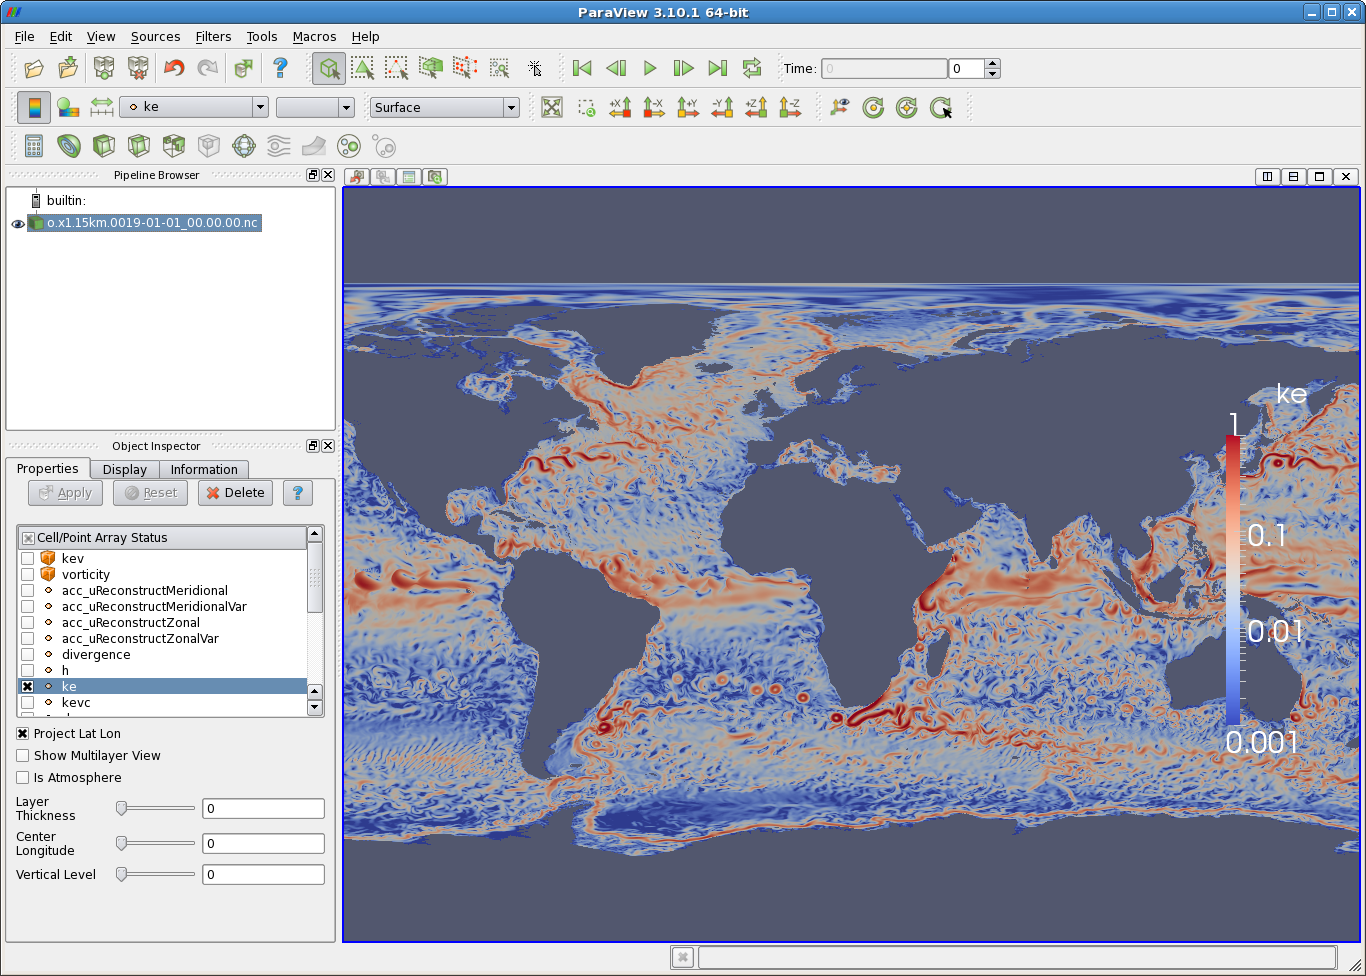
\includegraphics[width=6.5in]{shared/figures/ParaviewExample.png}
\caption{Example of ParaView to view an MPAS NetCDF file.}
\label{fig:ParaviewExample}
\end{center}
\end{figure}


\part{MPAS-Seaice}

% Grid generation is not included in MPAS release 1.0.
% In a future release, describe here ocean-specific grid
% generation, currently the basin.F program.
%\appendix{Generating meshes}
\label{chap:mpas_grid_generation}

This chapter describes the steps used to create the  spherical centroidal Voronoi tessellation (SCVT) meshes and mesh-decomposition files used by MPAS models.
Since it can take considerable time (often several days or more) to generate a mesh as described in \S \ref{sec:global_scvt}, it is recommended to obtain 
and use existing SCVT meshes from \url{http://www.mmm.ucar.edu/people/duda/mpas/} whenever possible; these meshes can be quickly
modified to shift or rotate the refinement regions over the geographic areas of interest using the utility program described in \S \ref{sec:grid_rotate}.

\section{Density functions}

In all MPAS models, the horizontal meshes are SCVTs with a C-grid staggering of
velocities. As their name suggests, SCVTs are Voronoi tessellations defined on the surface of a sphere, and in which the generating 
point for each Voronoi region is also the mass centroid of that region with respect to some {\em density function}. An overview of
the application of SCVTs to multi-resolution climate modeling is given in Ringler et al. (2008)
\footnote{Ringler, T., L. Ju and M. Gunzburger, 2008, A multiresolution method for climate system modeling: application of spherical centroidal Voronoi tessellations, {\em Ocean Dynamics}, 58 (5-6), 475-498. doi:10.1007/s10236-008-0157-2.}.

For the purposes of generating SCVTs, the central concern lies with the density function, $\rho$, which is a user-defined
function relating the relative resolutions in different regions of the mesh. Specifically, for two generating points of the 
SCVT, ${\bf x}_i$ and ${\bf x}_j$,
\[
{h_i \over h_j} \approx \left({\rho({\bf x}_j) \over \rho({\bf x}_i)} \right)^{1 \over 4},
\]
where $h_i$ and $h_j$ are the diameters of the Voronoi cells associated with ${\bf x}_i$ and ${\bf x}_j$, respectively.

In the mesh generation program global\_scvt, described in the next section, the density function is defined programatically in the Fortran function
{\tt density\_for\_point()}, which returns the value of the density function, $\rho({\bf x})$, given a location on the sphere, ${\bf x}$.
   
\section{The global\_scvt program}
\label{sec:global_scvt}

\subsection{Compilation}
                                                                                             
As a first step toward building the global\_scvt code, the environment variable                     
{\tt NETCDF} must be set to the root of the netCDF installation. Unlike with the MPAS model, separate make targets are not
defined for each compiler set, and it will generally be necessary to edit the top-level Makefile to set the compiler and compiler flags                 
that will be used to build global\_scvt; however, there are commented-out sections in the Makefile for using either of the ifort, pgf90, or gfortran compilers that may be uncommented or used as a starting point for other compilers. Also, if the netCDF installation has a separate Fortran interface library, {\tt -lnetcdff} will need to be added before {\tt -lnetcdf} in the Makefile. The global\_scvt program is parallelized with OpenMP, so if compiler support is available, OpenMP compiler flags may be added
in the Makefile as well.                      

Before compiling the global\_scvt program, a density function should first be defined in the function {\tt density\_for\_point()} in {\tt src/module\_scvt.F}. The default density function is a uniform density function that returns a value of 1.0 for all locations
on the sphere, and commented code in {\tt density\_for\_point()} may be uncommented to achieve an area of circular refinement. {\em Note that, although $\rho({\bf x})$ could in principle take on any non-negative value, the code to scale eddy viscosities by the mesh resolution in the MPAS model assumes that $\rho({\bf x}) \in (0,1]$, so care should be taken when designing a new density function: a value of 1.0 should correspond to the highest-resolution regions(s) in the mesh.}                                      
                                                                                                
After editing the Makefile and defining the desired density function, running `make' should create the grid\_gen executable 
in the top-level directory. A second program, grid\_ref, may also be created, but this program is not needed by the current version 
of the global\_scvt program.

\subsection{Running}

As will be described in Section \ref{sec:grid_gen_efficiency}, a typical mesh is generated using multiple refinement steps. Within each of these steps, an SCVT with a fixed
number of generating points is converged before the SCVT is refined, giving a larger number of generating points to begin the next step. In this section, the process of converging an SCVT within a single step is described.

Two files are needed in order to run the grid\_gen program: an initial generating point file, {\tt locs.dat}, and a                        
namelist file, {\tt namelist.input}. The {\tt locs.dat} file contains a list of the Cartesian coordinates (assuming a unit-radius sphere
centered at the origin) of each of the beginning generating points, and the {\tt namelist.input} file specifies the number of generating points to be read from the {\tt locs.dat} file, the number of iterations to run, and the convergence criteria; a complete list of namelist variables is provided in the table below.

\vspace{12pt}
\begin{longtable}{|p{1.25in} |p{4.5in}|}
\hline
np & the number of points to read from the {\tt locs.dat} file \\ \hline
locs\_as\_xyz & whether the initial generating points in {\tt locs.dat} are given in Cartesian space ({\tt .true.}) or latitude-longitude space ({\tt .false.}) \\ \hline
n\_scvt\_iterations & the maximum number of Lloyd iterations to perform \\ \hline
eps & the convergence criterion, specifying the maximum permissible average movement of a generating point during an iteration \\ \hline
l2\_conv & whether to stop iterating if the convergence criterion is met \\ \hline
inf\_conv & currently the same meaning as l2\_conv \\ \hline
min\_dx & the targeted minimum grid distance in the mesh, on which an estimate for the number of generating points will be based; see Section \ref{sec:estimating_np} \\ \hline
\end{longtable}
\vspace{12pt}

\noindent A convergence criterion of $1\times10^{-10}$ should be sufficient, and in                     
practice, many thousands of iterations are needed to reach this tolerance.

If grid\_gen was compiled with OpenMP support, the environment variable {\tt OMP\_NUM\_THREADS} can be set to the 
number of threads that will be used by the program. Then, grid\_gen can be run with no command-line arguments:

\vspace{12pt}
{\tt > ./grid\_gen}
\vspace{12pt}
                                                                                         
                                                                                                
When grid\_gen finishes --- either because the convergence criterion has been met, or the
maximum number of iterations have been performed ---  several output files should be created: 

\begin{itemize}
\item {\tt scvt\_initial.ps} --- a plot of the mesh at the start of iterations,
\item {\tt scvt\_final.ps} --- a plot of the mesh after iterations,
\item {\tt grid.nc} --- the actual MPAS mesh file, which can be used with the initialization core to create an MPAS input file,
\item {\tt graph.info} --- information describing the cell connectivity graph of the mesh, to be used with a graph partitioner as described in Section \ref{sec:metis}, and
\item {\tt locs.dat.out} --- a list of the final generating points appended with a set of $3 np - 6$ refinement points. 
\end{itemize}

If the tolerance specified in the {\tt namelist.input} file was met, the SCVT mesh should be sufficiently converged, and the resulting {\tt grid.nc}
file can be used with the initialization program to create an initial condition file for MPAS; alternatively, the full set of $4 np - 6$ refinement points in 
the {\tt locs.dat.out} file can be used as input to the grid\_gen program to create another SCVT with approximately twice the resolution. If, however, the specified tolerance was not met, the {\tt locs.dat.out} file may be copied to {\tt locs.dat}, and further iteration may be performed on the SCVT.

To create a plot of the mesh with coastlines, which can be helpful when locating or sizing refinement regions, the {\tt mesh.ncl} script may be used to plot the mesh directly from                 
the {\tt grid.nc} file.                                                                          

\subsection{Estimating the required number of generating points}
\label{sec:estimating_np}

Setting the {\tt min\_dx} variable in the {\tt namelist.input} file to the targeted minimum grid distance in the mesh and running the grid\_gen program will cause the program to print out an estimate for the number of generating points that will be required to achieve that minimum grid distance with the density function provided in {\tt density\_for\_point()}.

\subsection{Efficiency concerns}
\label{sec:grid_gen_efficiency}

Although one could, given an estimate for the number of generating points needed to achieve the required absolute resolutions in the mesh,
create a {\tt locs.dat} file with that number of randomly chosen points on the unit sphere, and, using that {\tt locs.dat} file, converge a final SCVT, 
experience indicates that a stepwise approach can significantly reduce the required wallclock time.                   

   
\section{The grid\_rotate program} 
\label{sec:grid_rotate} 

The purpose of the grid\_rotate program is simply to rotate an MPAS mesh file, moving a refinement region from one geographic location to another, so that the mesh can be re-used for different applications. This utility was developed out of the need to save computational resources, since generating an SCVT --- particularly one with a large number of generating points or a high degree of refinement --- can take considerable time.

To build the grid\_rotate program, the Makefile should first be edited to set the Fortran compiler to be used; if the netCDF installation pointed to by the {\tt NETCDF} environment variable was build with a separate Fortran interface library, it will also be necessary to add {\tt -lnetcdff} just before {\tt -lnetcdf} in the Makefile. After editing the Makefile, running `make' should result in a grid\_rotate executable file.

Besides the MPAS grid file to be rotated, grid\_rotate requires a namelist file, {\tt namelist.input}, which specifies the rotation to be applied to the mesh. The namelist variables are summarized in the table below
   
\vspace{12pt}
\begin{longtable}{|p{3.25in} |p{2.5in}|}
\hline
config\_original\_latitude\_degrees & original latitude of any point on the sphere \\ \hline
config\_original\_longitude\_degrees & original longitude of any point on the sphere \\ \hline
config\_new\_latitude\_degrees &  latitude to which the original point should be shifted \\ \hline
config\_new\_longitude\_degrees &  longitude to which the original point should be shifted \\ \hline
config\_birdseye\_rotation\_counter\_clockwise\_degrees & rotation about a vector from the sphere center through the original point \\ \hline
\end{longtable}
\vspace{12pt}

\noindent Essentially, one chooses any point on the sphere, decides where that point should be shifted to,
and specifies any change to the orientation (i.e., rotation) of the mesh about that point. 

Having set the rotation parameters in the {\tt namelist.input} file, the grid\_rotate program should be run with two command-line options
specifying the original grid file name and the name of the rotated grid file to be produced, e.g.,

\vspace{12pt}
{\tt > grid\_rotate grid.nc grid\_SE\_Asia\_refinement.nc}
\vspace{12pt}

The original grid file will not be altered, and a new, rotated grid file will be created. The NCL script {\tt mesh.ncl} may be used to plot either of the original or rotated grid files after suitable setting the name of the grid file in the script.
   
   
\section{Graph partitioning with METIS} 
\label{sec:metis}

{\color{red} THIS SECTION WAS COPIED TO mpas_build_instructions.tex  FOR RELEASE 1.0. WHEN GRID GENERATION IS INCLUDED, DELETE THE METIS SECTION FROM mpas_build_instructions.tex}.

Before MPAS can be run in parallel, a mesh decomposition file with an appropriate number of 
partitions (equal to the number of MPI tasks that will be used) is required in the run directory.  A limited number of mesh decomposition files ({\tt graph.info.part.*}) are provided with each test case (see Test Cases Chapter).  In order to create new mesh decomposition files for your desired number of partitions, begin with the {\tt graph.info} file created by the grid\_gen program or available with your test case, and partition with METIS software (\url{http://glaros.dtc.umn.edu/gkhome/views/metis}). The serial graph partitioning program, METIS (rather than ParMETIS or hMETIS) should be sufficient for quickly partitioning any SCVT produced by the grid\_gen mesh generator.

After installing METIS, a {\tt graph.info} file may be partitioned into $N$ partitions by running

\vspace{12pt}
{\tt > gpmetis graph.info} $N$
\vspace{12pt}

\noindent The resulting file, {\tt graph.info.part.}$N$, can then be copied into the MPAS run directory
before running the model with $N$ MPI tasks.



\chapter{Model Description}
\label{chap:model_description}

\section{Velocity Solver}
\label{sec:velocity_solver}

\subsection{Overview}

MPAS-Seaice uses a `B' Arakawa type grid \citep{Arakawa77} with both components of velocity defined at cell vertices and sea-ice concentration, volume and other tracers defined at cell centers (see Chapter \ref{chap:mpas_grid_description}). When using CICE-like quadrilateral meshes, this allows the velocity solver algorithm of MPAS-Seaice to reduce to that of CICE, allowing CICE and MPAS-Seaice to use identical test cases and allow rapid testing and development. 

In CICE the velocity components are aligned with the quadrilateral mesh. This is not possible, in general, with MPAS-Seaice since a SCVT MPAS mesh does not have edges with perpendicular directions as in a quadrilateral mesh. Instead, the velocity components at a given MPAS vertex are defined as eastwards ($u$) and northwards ($v$), irrespective of the orientation of edges joining that vertex. Such a definition, however, would result in a convergence of $v$ components at the geographic North Pole and strong metric terms in the velocity solution. Consequently, in addition, we rotate these definitions of $u$ and $v$ so that their pole lies on the geographical equator at $0^\circ$ longitude. 

To prognose sea-ice velocity we solve the same sea-ice momentum equation as CICE \citep{Hibler79,Hunke97}:
\begin{equation}
m \frac{\partial{\boldsymbol{u}}}{\partial{t}} = \boldsymbol{\nabla} \cdot \boldsymbol{\sigma} + \boldsymbol{\tau_a} + \boldsymbol{\tau_w} - \boldsymbol{\hat{k}} \times m f \boldsymbol{u} -mg \boldsymbol{\nabla}H_o.
\end{equation}
Here $m$ is the mass of snow and ice per unit area, $\boldsymbol{u}$ is the sea-ice velocity, $\boldsymbol{\sigma}$ is the ice internal stress tensor, $\boldsymbol{\tau_a}$ and $\boldsymbol{\tau_w}$ are the horizontal stresses due to atmospheric winds and ocean currents respectively, $\boldsymbol{\hat{k}}$ is the unit vector normal to the Earth surface, $f$ is the Coriolis parameter, $g$ is the acceleration due to gravity and $H_o$ is the ocean surface height. The second to last term represents the Coriolis force and the last term represents the force due to the ocean surface tilt. Only the divergence of internal stress and ocean surface tilt terms depend on horizontal differential operators. During coupled simulations the ocean model provides the ocean surface tilt term, whereas in non-coupled simulations we assume that the ocean currents are in geostrophic balance so that
\begin{equation}
mg \boldsymbol{\nabla}H_o = m f \boldsymbol{\hat{k}} \times \boldsymbol{u_o}
\end{equation}
where $\boldsymbol{u_o}$ is the ocean surface velocity. Consequently, only the divergence of internal stress depends on the properties of the horizontal grid employed, and only adaptations to this stress term are required to adapt the velocity solver of CICE to MPAS meshes. The other terms in the momentum equation are solved in an identical way to CICE.

Determination of the divergence of the internal stress can be broken down into three stages: 
\begin{enumerate}
\item The strain rate tensor is determined from the velocity field.
\item The stress tensor at a point is determined, through a constitutive relation, from the strain rate tensor at that point.
\item The divergence of this stress tensor is calculated. 
\end{enumerate}
As in CICE we use an Elastic-Viscous-Plastic (EVP) rheology \citep{Hunke97} for the constitutive relation. This step does not depend on the details of the horizontal mesh and we use the same formulation as CICE. We develop two schemes to calculate the strain rate tensor and the divergence of internal stress on MPAS meshes. A variational scheme is based on that used in CICE \citep{Hunke02}, whereas a weak scheme uses the line integral forms of the symmetric gradient and divergence operators. These schemes are described in the following sections.

\subsection{Variational Scheme}

We develop a variational scheme for calculating the divergence of stress based on that of \citet{Hunke02} but adapted for arbitrarily shaped and sided convex polygons. This scheme is based on the fact that over the entire domain, $\Omega$, and ignoring boundary effects, the total work done by the internal stress is equal to the dissipation of mechanical energy:
\begin{equation}
\int_\Omega \boldsymbol{u} \cdot (\boldsymbol{\nabla} \cdot \boldsymbol{\sigma}) \mathrm{d}A = -\int_\Omega (\boldsymbol{\sigma_{11}} \boldsymbol{\dot{\epsilon}_{11}}  + 2 \boldsymbol{\sigma_{12}} \boldsymbol{\dot{\epsilon}_{12}} + \boldsymbol{\sigma_{22}} \boldsymbol{\dot{\epsilon}_{22}}) \mathrm{d}A.
\label{eqn:work_done}
\end{equation}
Here $\boldsymbol{\dot{\epsilon}}$ is the strain rate tensor and the integrals are area integrals over the whole model domain. The work done over the whole domain can be split into a sum over the contribution to the work done from each cell on the dual Delaunay mesh. Each dual cell on the dual mesh consists of a triangle surrounding a single vertex point where the discretized velocity is defined. Equation \ref{eqn:work_done} can then be written as
\begin{equation}
\sum_i^{n_d} \int_i \boldsymbol{u} \cdot (\boldsymbol{\nabla} \cdot \boldsymbol{\sigma}) \mathrm{d}A = D(u_1, u_2, ..., u_n, v_1, v_2, ..., v_{n_d})
\end{equation}
where the left-side sum is over the $n_d$ cells of the dual mesh, the integral is an area integral over each dual cell,  and the dissipation of mechanical energy has been written as a function of the discretized velocity components.
Writing the two components of the divergence of stress as $F_u=(\nabla \cdot \sigma)_u$ and $F_v=(\nabla \cdot \sigma)_v$, then
\begin{equation}
\sum_i^{n_d} \int_i (uF_u + vF_v) \mathrm{d}A = D(u_1, u_2, ..., u_n, v_1, v_2, ..., v_{n_d}).
\end{equation}
If we assume that within the dual cell the velocity is constant, it follows that
\begin{equation}
\sum_i^{n_d} (u_i F_{ui} + v_i F_{vi}) A_{ui} = D(u_1, u_2, ..., u_n, v_1, v_2, ..., v_{n_d})
\end{equation}
where $A_{ui}$ is the area of the dual mesh cell.
The variation of these expressions with respect to the $u$ component of the discretized velocity at a particular vertex point $j$ is given by
\begin{equation}
\frac{\partial{}}{\partial{u_j}} \sum_i^{n_d} (u_i F_{ui} + v_i F_{vi}) A_{ui} =  \frac{\partial{}}{\partial{u_j}}D(u_1, u_2, ..., u_n, v_1, v_2, ..., v_{n_d})
\end{equation}
Assuming $F_u$ and $F_v$ are not functions of velocity,
\begin{equation}
F_{uj} =  \frac{1}{A_{uj}} \frac{\partial{}}{\partial{u_j}}D(u_1, u_2, ..., u_n, v_1, v_2, ..., v_{n_d}).
\label{eqn:variation}
\end{equation}
$F_v$ is obtained in a similar way by taking the variation of $D$ with respect to $v_j$. The dissipation of mechanical energy, $D$, can be split into three terms: 
\begin{equation}
D=D_1+ D_2+D_3
\end{equation}
with
\begin{equation}
D_1=-\int  \boldsymbol{\sigma_{11}} \boldsymbol{\dot{\epsilon}_{11}} \mathrm{d}A ,\quad D_2=-\int  2 \boldsymbol{\sigma_{12}} \boldsymbol{\dot{\epsilon}_{12}} \mathrm{d}A, \quad D_3=-\int  \boldsymbol{\sigma_{22}} \boldsymbol{\dot{\epsilon}_{22}} \mathrm{d}A.
\end{equation}
We will calculate the contribution to $F_u$ and $F_v$ from $D_1$. Similar contributions come from $D_2$ and $D_3$. Using the expression for $\dot{\epsilon}_{11}$ in terms of the velocity components and latitude $\phi$, $D_1$ becomes
\begin{equation}
D_1=-\int  \sigma_{11} \left[ \frac{\partial{u}}{\partial{x}} - \frac{v \tan{\phi}}{r} \right] \mathrm{d}A
\end{equation}
where $x$ and $y$ are locally Cartesian coordinates, with $x$ in the rotated due eastwards direction and $y$ in the rotated due northwards direction, $\phi$ is the latitude, and $r$ is the radius of the Earth. The second term in $\dot{\epsilon}$ accounts for the metric effects of the curved domain \citep{Batchelor67}.
The integral can be broken up into a sum over the $n_p$ cells in the primary mesh:
\begin{equation}
D_1=- \sum_k^{n_p} \int_k  \sigma_{11} \left[ \frac{\partial{u}}{\partial{x}} - \frac{v \tan{\phi}}{r} \right] \mathrm{d}A
\label{eqn:d_1}
\end{equation}
where the integral is over the interior area of the $k$th cell. 
To perform this integral we use a set of basis functions, $\mathcal{W}_l$, to represent functions within a cell of the primary mesh. If a function, $\psi$, has a value of  $\psi_l$ at vertex $l$ of a cell, then the value of the function at a position $(x,y)$ within the cell can be approximated as
\begin{equation}
\psi(x,y) = \sum_l^{n_v} \psi_l \mathcal{W}_l (x,y)
\end{equation}
where the sum is over the $n_v$ vertices of the cell in the primary mesh.
Using those basis functions, equation \ref{eqn:d_1} can be written as 
\begin{equation}
D_1=-\sum_k^{n_p} \int_k \left[ \sum_{l}^{n_v} \sigma_{11{l}} \mathcal{W}_{l} \cdot \sum_{m}^{n_v} \left(u_{m} \frac{\partial{\mathcal{W}_{m}}}{\partial{x}} - \frac{\tan{\phi}}{r} v_{m} \mathcal{W}_{m} \right) \right]\mathrm{d}A
\end{equation}
where the derivative with respect to $x$ has been taken inside the summation.
Rearranging
\begin{equation}
D_1= -\sum_k^{n_p} \sum_{l}^{n_v} \sum_{m}^{n_v} \sigma_{11{l}}\left( u_{m} \int_k  \mathcal{W}_{l}   \frac{\partial{\mathcal{W}_{m}}}{\partial{x}}  \mathrm{d}A  - \frac{\tan{\phi}}{r}  v_{m} \int_k \mathcal{W}_{l} \mathcal{W}_{m}  \mathrm{d}A  \right).
\end{equation}
In moving the integral, we have assumed that $\phi$, the latitude, is constant in the cell. The terms involving integrals are now only a function of the geometry of the mesh and can be calculated once during the initialization phase of the model run. Defining 
\begin{equation}
\mathcal{S}^x_{lm} = \int_k  \mathcal{W}_{l}   \frac{\partial{\mathcal{W}_{m}}}{\partial{x}}  \mathrm{d}A
\end{equation}
and
\begin{equation}
\mathcal{T}_{lm} = \int_k \mathcal{W}_{l} \mathcal{W}_{m}  \mathrm{d}A.
\end{equation}
we have
\begin{equation}
D_1= -\sum_k^{n_p} \sum_{l}^{n_v} \sum_{m}^{n_v} \sigma_{11{l}}\left( u_{m} \mathcal{S}^x_{lm}  - \frac{\tan{\phi}}{r}  v_{m} \mathcal{T}_{lm}  \right).
\end{equation}
Taking the variation with respect to a discretized velocity component at a particular vertex point, $j$, as in equation \ref{eqn:variation}, now gives us the contribution from $D_1$ to the components of the divergence of stress tensor at that velocity point:
\begin{equation}
(\nabla \cdot \sigma)_{u_j}^{D_1} = \frac{\delta D_1}{\delta u_{j}}= -\sum_k^{n_p} \sum_{l}^{n_v}  \sigma_{11{l}} \mathcal{S}^x_{lj}
\end{equation}
\begin{equation}
(\nabla \cdot \sigma)_{v_j}^{D_1} = \frac{\delta D_1}{\delta v_{j}}= \sum_k^{n_p} \sum_{l}^{n_v}  \sigma_{11{l}}  \frac{\tan{\phi}}{r} \mathcal{T}_{lj}
\end{equation}
Only cells that border the vertex point $j$ contribute to the $k$ sum over cells. The total divergence of stress at the point $j$ is then the sum from the contributions from $D_1$, $D_2$, and $D_3$:
\begin{equation}
(\nabla \cdot \sigma)_{u_j} = (\nabla \cdot \sigma)_{u_j}^{D_1} + (\nabla \cdot \sigma)_{u_j}^{D_2} + (\nabla \cdot \sigma)_{u_j}^{D_3}
\end{equation}
\begin{equation}
(\nabla \cdot \sigma)_{v_j} = (\nabla \cdot \sigma)_{v_j}^{D_1} + (\nabla \cdot \sigma)_{v_j}^{D_2} + (\nabla \cdot \sigma)_{v_j}^{D_3}.
\end{equation}
All that remains now is to determine the stress for each cell at its vertices. As in the formulation in CICE, each cell has its own values of the stress at its vertices, so each vertex has several values of the stress, each corresponding to a different surrounding cell. The stresses are calculated from the strain rate tensor at each vertex using the constitutive relation. Including metric effects \citep{Batchelor67} the strain rate tensor is given by:
\begin{equation}
\dot{\epsilon}_{11} = \frac{\partial{u}}{\partial{x}} - \frac{v \tan{\phi}}{r}
\end{equation}
\begin{equation}
\dot{\epsilon}_{22} = \frac{\partial{v}}{\partial{y}}
\end{equation}
\begin{equation}
\dot{\epsilon}_{12} = \frac{1}{2} \left( \frac{\partial{u}}{\partial{y}} + \frac{\partial{v}}{\partial{x}} \right) + \frac{u \tan{\phi}}{2 r}.
\end{equation}
The strain rate tensor at cell vertex $l$ is then given by 
\begin{equation}
\dot{\epsilon}_{11{l}} =  \sum_{m}^{n_v} u_{m} \left. \frac{\partial{\mathcal{W}_{m}}}{\partial{x}} \right| _{l} - \frac{v_{l} \tan{\phi_{l}}}{r}
\end{equation}
\begin{equation}
\dot{\epsilon}_{22{l}} =  \sum_{m}^{n_v} v_{m} \left. \frac{\partial{\mathcal{W}_{m}}}{\partial{y}} \right| _{l} 
\end{equation}
\begin{equation}
\dot{\epsilon}_{12{l}} = \frac{1}{2} \left( \sum_{m}^{n_v} u_{m} \left. \frac{\partial{\mathcal{W}_{m}}}{\partial{y}} \right| _{l} +\sum_{m}^{n_v} v_{m} \left. \frac{\partial{\mathcal{W}_{m}}}{\partial{x}} \right| _{l}  \right) + \frac{u_{l} \tan{\phi_{l}}}{2 r}
\end{equation}
The derivatives of the basis functions are taken at cell vertex $l$.

In MPAS-Seaice we provide two options for the choice of basis functions, $\mathcal{W}_l$: Wachspress basis functions and Piece-Wise Linear (PWL) basis functions. Both basis functions have a value of one on vertex $l$ and zero on the other vertices of a cell, and are linear on the cell boundaries. The Wachspress basis functions are smooth rational polynomials in the cell interior \citep{Dasgupta03}. The integrals of the Wachspress basis function within a cell are performed using the eighth order quadrature rules of \citet{Dunavant85}. PWL basis functions divide the polygonal cell into sub-triangles and use a linear basis within each sub-triangle \citep{Bailey08}. To divide the polygonal cell into sub-triangles, a point is chosen within the cell and sub-triangles formed using this point and two adjacent vertices. The central point in the cell, $\mathbf{x}_c$,  is chosen as
\begin{equation}
\mathbf{x}_c = \sum_i^{n_v} \alpha_i \mathbf{x}_i
\end{equation}
where the sum is over the $n_v$ vertices of the cell each with position $\mathbf{x}_i$. The simplest choice for the $\alpha_i$ is to set them all equal to the inverse of the number of cell vertices, $1/n_v$. For quadrilateral meshes the Wachspress basis functions reduce to the bilinear basis functions used in CICE.

\subsection{Weak Scheme}

\begin{figure}[]
\centering
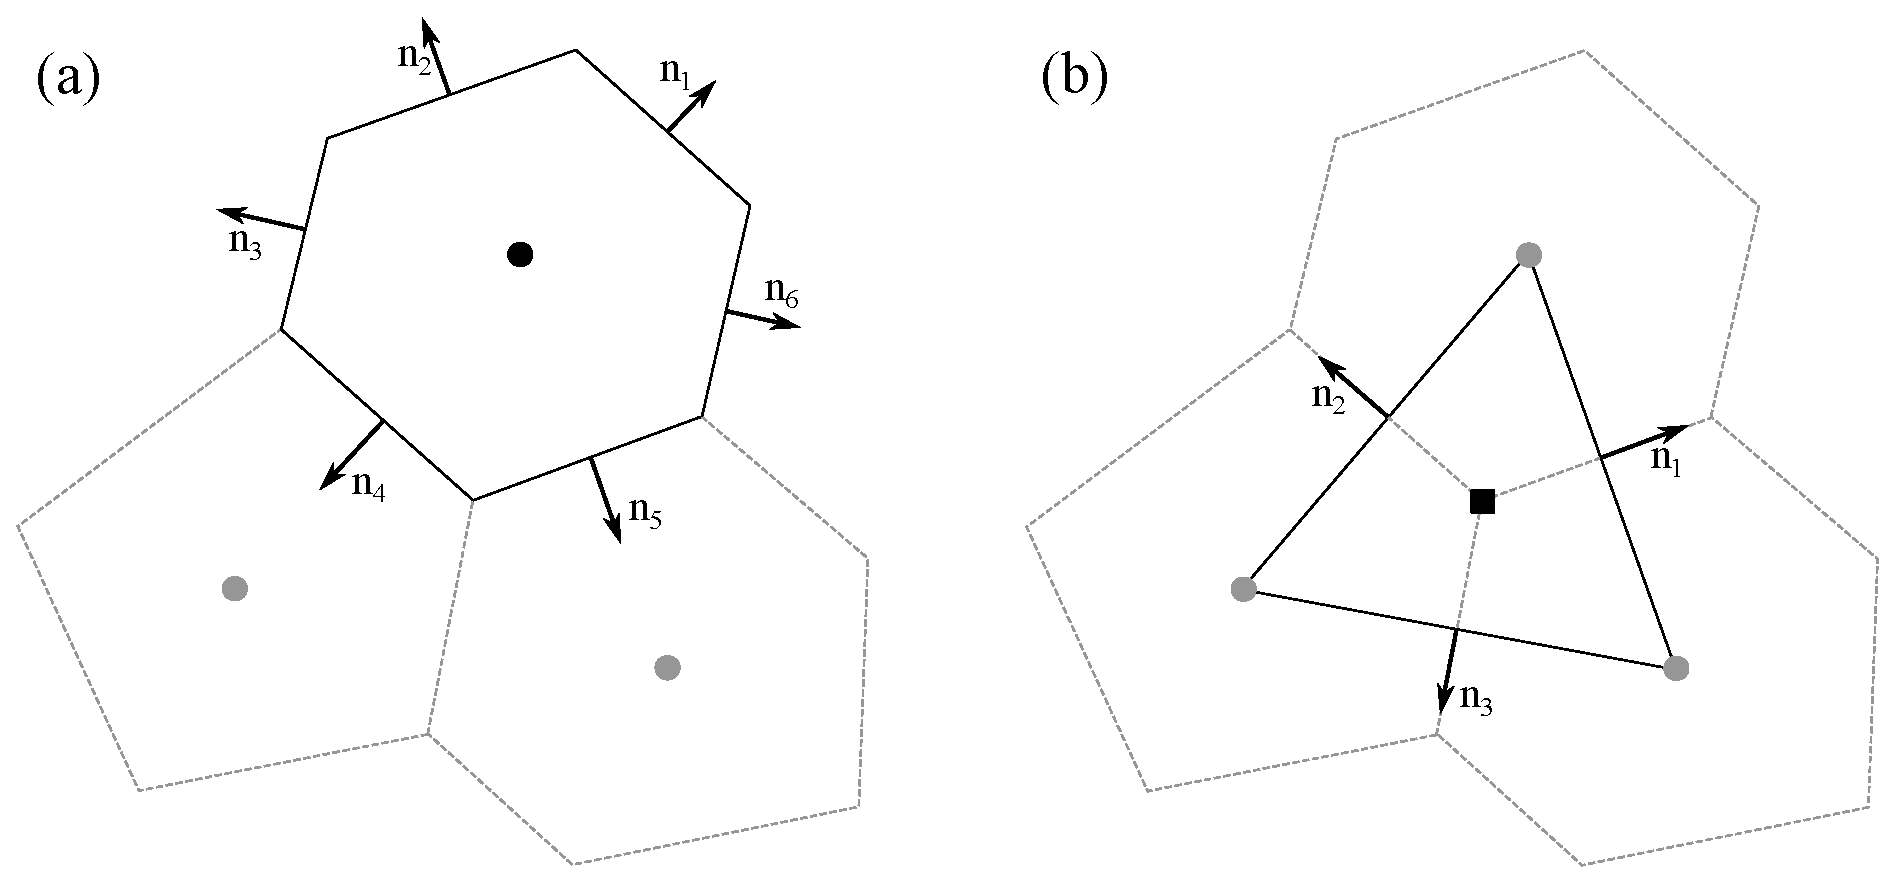
\includegraphics[width=\linewidth]{seaice/figures/mesh_weak.eps}
\caption{Contour integration lines used by the weak scheme. (a): Strain rate at cell centers (\emph{circle}) are calculated from line integrals around primary mesh cells (\emph{solid line}). (b): Divergence of stress at cell vertices (\emph{square}) are calculated from line integrals around the dual mesh cells (\emph{solid line}). Directions of normal vectors used in the integrals are shown for both figures.}
\label{fig:mesh_weak}
\end{figure}

For the weak scheme we use line integrals around cells in the primary and dual meshes to calculate the strain rate tensor and the divergence of stress, respectively. To determine the strain rate tensor we start from the following vector identity:
\begin{equation}
\boldsymbol{\nabla} \cdot (\boldsymbol{u} \otimes \boldsymbol{v}) = (\boldsymbol{u} \cdot \boldsymbol{\nabla}) \boldsymbol{v} + (\boldsymbol{\nabla} \cdot \boldsymbol{u}) \boldsymbol{v}
\label{eqn:vector_identity}
\end{equation}
and from the divergence theorem:
\begin{equation}
\int_\Omega \left[ \boldsymbol{\nabla} \cdot (\boldsymbol{u} \otimes \boldsymbol{v}) \right] \partial{\Omega} = \oint_S \left[\boldsymbol{n} \cdot (\boldsymbol{u} \otimes \boldsymbol{v}) \right] \partial{S} = \oint_S \left[(\boldsymbol{n} \cdot \boldsymbol{u}) \boldsymbol{v} \right] \partial{S}
\label{eqn:divergence_theorem}
\end{equation}
where $\boldsymbol{n}$ is a normal vector to the surface $S$ and $\otimes$ is the tensor product.
If equation \ref{eqn:vector_identity} is integrated over $\Omega$, using equation \ref{eqn:divergence_theorem} we obtain
\begin{equation}
\int_\Omega \left[ (\boldsymbol{u} \cdot \boldsymbol{\nabla}) \boldsymbol{v} + (\boldsymbol{\nabla} \cdot \boldsymbol{u}) \boldsymbol{v} \right] \partial{\Omega} = \oint_S \left[(\boldsymbol{n} \cdot \boldsymbol{u}) \boldsymbol{v} \right] \partial{S}
\label{eqn:weak1}
\end{equation}
If $\boldsymbol{u}$ is chosen as constant then $\boldsymbol{\nabla} \cdot \boldsymbol{u}$ vanishes as does the second term in equation \ref{eqn:weak1}. Taking, also, $\boldsymbol{u}$ sequentially as the cartesian unit vectors spanning $\Omega$ and summing the results we obtain
\begin{equation}
\int_\Omega \left[ \boldsymbol{\nabla} \boldsymbol{v} \right] \partial{\Omega} = \oint_S \left[ \boldsymbol{n} \otimes \boldsymbol{v} \right] \partial{S}
\end{equation}
The symmetric version of this operator is then obtained as:
\begin{equation}
\int_\Omega \left[ \boldsymbol{\nabla_S} \boldsymbol{v} \right] \partial{\Omega} = \oint_S \left[ \boldsymbol{n} \otimes \boldsymbol{v} + \boldsymbol{v} \otimes \boldsymbol{n} \right] \partial{S}
\end{equation}
The strain rate at a point is then obtained from the limit
\begin{equation}
\boldsymbol{\dot{\epsilon}} = \boldsymbol{\nabla}_S \boldsymbol{v} = \lim_{A \to 0} \frac{1}{A} \oint \frac{1}{2}\left[ \boldsymbol{n} \otimes \boldsymbol{v} + \boldsymbol{v} \otimes \boldsymbol{n} \right] \mathrm{d}l
\end{equation}
where the integral is around a closed loop with area $A$ and normal vector $\boldsymbol{n}$, and $\boldsymbol{v}$ is the sea-ice velocity.
To determine the strain rate tensor at the centers of the primary mesh, we take this integration around the edges of the cells in the primary mesh. First the cell is projected onto a flat tangent plane perpendicular to the vector joining the center of the sphere to the cell center. We take the sea ice velocity at a cell edge as the average of the values on the two vertices forming that edge projected onto the tangent plane:
\begin{equation}
\boldsymbol{\dot{\epsilon}}^\prime = \frac{1}{A} \sum_i^{n_e} \frac{1}{2} \left[ \boldsymbol{n}_i \otimes \boldsymbol{v}_i + \boldsymbol{v}_i \otimes \boldsymbol{n}_i \right] l_i
\end{equation}
Here, $A$ is the area of the primary cell, the summation is over the $n_e$ edges of the primary cell, $\boldsymbol{n}_i$ is the normal vector to the edge $i$ that lies in the tangent plane, $\boldsymbol{v}_i$ is the edge velocity and $l_i$ is the length of edge $i$. We use the tangental projection of the velocity and account for metric terms separately. The full strain rate tensor including these metric terms is \citep{Batchelor67}:
\begin{equation}
\dot{\epsilon}_{11} = \dot{\epsilon}_{11}^\prime - \frac{v \tan{\phi}}{r}
\end{equation}
\begin{equation}
\dot{\epsilon}_{22} = \dot{\epsilon}_{22}^\prime
\end{equation}
\begin{equation}
\dot{\epsilon}_{12} = \dot{\epsilon}_{12}^\prime + \frac{u \tan{\phi}}{2r}
\end{equation}
where the prime symbol signifies a strain rate without metric terms.
The stress, which is determined from the strain rate tensor using the constitutive relation, is now defined on cell centers. To find its divergence we use the divergence theorem:
\begin{equation}
\iint \boldsymbol{\nabla} \cdot \boldsymbol{\sigma} \mathrm{d}A = \oint \left[ \boldsymbol{\sigma} \cdot \boldsymbol{n} \right] \mathrm{d}l
\end{equation}
or
\begin{equation}
\boldsymbol{\nabla} \cdot \boldsymbol{\sigma} = \lim_{A \to 0}  \frac{1}{A} \oint \left[ \boldsymbol{\sigma} \cdot \boldsymbol{n} \right] \mathrm{d}l
\end{equation}
for the divergence of stress at a point.
The divergence of internal stress is determined at primary cell vertices (where the velocity is defined and momentum equation solved) by performing a sum around the edges of the dual mesh on a tangent projected plane, tangental to the primary cell vertex. The vertices of the dual mesh are the cell centers of the primary mesh where the strain rate has been determined. The divergence of stress at primary cell vertices is then given by
\begin{equation}
(\boldsymbol{\nabla} \cdot \boldsymbol{\sigma})^\prime = \frac{1}{A_d} \sum_i^{n_c} \left[ \boldsymbol{\sigma}_i \cdot \boldsymbol{n}_i \right] l_i
\end{equation}
where $A_d$ is the area of the dual mesh cell, the sum is over the $n_c$ vertices of the dual mesh, $l_i$ is the length of the $i$ edge of the dual mesh, and $n_i$ is a normal vector to the $i$ edge on the projected plane. As before, this gives a result without taking into account metric effects of the mesh. With those effects the divergence of stress is:
\begin{equation}
(\nabla \cdot \sigma)_u = (\nabla \cdot \sigma)_u^\prime - \frac{2 \sigma_{12} \tan{\phi}}{r}
\end{equation}
\begin{equation}
(\nabla \cdot \sigma)_v = (\nabla \cdot \sigma)_v^\prime + \frac{(\sigma_{11} + \sigma_{22}) \tan{\phi}}{r}
\end{equation}
where the components of $\boldsymbol{\sigma}$ are approximated as the
average of the values on the dual mesh vertices.

\section{Transport}
\label{sec:transport}

\label{describe_transport}

To transport sea ice fractional area and various tracers, MPAS-Seaice uses an incremental remapping (IR) algorithm similar to that described by \citet{Dukowicz00}, \citet{Lipscomb04} (henceforth LH04) and \citet{Lipscomb05} (henceforth LR05). The LH04 scheme was designed for structured quadrilateral meshes and is implemented in CICE \citep{Hunke15}. The LR05 scheme was implemented on a structured SCVT global mesh consisting of quasi-regular hexagons and 12 pentagons.

For MPAS-Seaice the IR scheme was generalized to work on either the standard MPAS mesh (hexagons and other n-gons of varying sizes, with a vertex degree of 3 as in LR05) or a quadrilateral mesh (with a vertex degree of 4 as in LH04 and CICE). Since MPAS meshes are unstructured, the IR scheme had to be rewritten from scratch. Most of the code is mesh-agnostic, but a small amount of code is specific to quad meshes as noted below.

Here we review the conceptual framework of incremental remapping as in \citep{Hunke15} and describe features specific to the MPAS-Seaice implementation. IR is designed to solve equations of the form
\begin{equation}
\label{eq:transport_m}
\frac{\partial m}{\partial t} =-\nabla \boldsymbol{\cdot} (\mathbf{u}m)
\end{equation}
\begin{equation}
\label{eq:transport_T1}
\frac{\partial (m T_1)}{\partial t} = -\nabla \boldsymbol{\cdot} (\mathbf{u} m T_1),
\end{equation}
\begin{equation}
\label{eq:transport_T2}
\frac{\partial (m T_1 T_2)}{\partial t} = -\nabla \boldsymbol{\cdot} (\mathbf{u} m T_1 T_2),
\end{equation}
\begin{equation}
\label{eq:transport_T3}
\frac{\partial (m T_1 T_2 T_3)}{\partial t} = -\nabla \boldsymbol{\cdot} (\mathbf{u} m T_1 T_2 T_3),
\end{equation}
where $\mathbf{u} = (x,y)$ is the horizontal velocity, $m$ is mass or a mass-like field (such as density or fractional sea ice concentration), and $T_1$, $T_2$ and $T_3$ are tracers.  These equations describe conservation of quantities such as mass and internal energy under horizontal transport. Sources and sinks of mass and tracers (e.g., ice growth and melting) are treated separately from transport.  

In MPAS-Seaice, the fractional ice area in each thickness category is a mass-like field whose transport is described by (\ref{eq:transport_m}). (Henceforth, ``area'' refers to fractional ice area unless stated otherwise.) Ice and snow thickness, among other fields, are type 1 tracers obeying equations of the form (\ref{eq:transport_T1}), and the ice and snow enthalpy in each vertical layer are type 2 tracers obeying equations like (\ref{eq:transport_T2}), with ice or snow thickness as their parent tracer. When run with advanced options (e.g., active melt ponds and biogeochemistry), MPAS-Seaice advects tracers up to type 3. Thus, the mass-like field is the ``parent field'' for type 1 tracers; type 1 tracers are parents of type 2; and type 2 tracers are parents of type 3.

Incremental remapping has several desirable properties for sea ice modeling:
\begin{itemize}
\item It is conservative to within machine roundoff.
\item It preserves tracer monotonicity.  That is, transport produces no new local extrema in fields like ice thickness or internal energy. 
\item The reconstructed mass and tracer fields vary linearly in x and y. This means that remapping is second-order accurate in space, except where gradients are limited locally to preserve monotonicity.
\item There are economies of scale.  Transporting a single field is fairly expensive, but additional tracers have a low marginal cost, especially when all tracers are transported with a single velocity field as in CICE and MPAS-Seaice.
\end{itemize}

The time step is limited by the requirement that trajectories projected backward from vertices are confined to the cells sharing the vertex (i.e., 3 cells for the standard MPAS mesh and 4 for the quad mesh).  This is what is meant by incremental as opposed to general remapping. This requirement leads to a CFL-like condition,
\begin{equation}
\label{eq:IR_CFL}
\frac{\max (|\mathbf{u}|\Delta t)}{\Delta x}\le 1,
\end{equation}
where $\Delta x$ is the grid spacing and $\Delta t$ is the time step. For highly divergent velocity fields, the maximum time step may have to be reduced by a factor of 2 to ensure that trajectories do not cross. 

The IR algorithm consists of the following steps:
\begin{itemize}
\item Given mean values of the ice area and tracer fields in each grid cell and thickness category, construct linear approximations of these fields. Limit the field gradients to preserve monotonicity.
\item Given ice velocities at grid cell vertices, identify departure regions for the transport across each cell edge. Divide these departure regions into triangles and compute the coordinates of the triangle vertices.
\item Integrate the area and tracer fields over the departure triangles to obtain the area, volume, and other conserved quantities transported across each cell edge.
\item Given these transports, update the area and tracers.
\end{itemize}
\noindent
Since all fields are transported by the same velocity field, the second step is done only once per time step. The other steps are repeated for each field.

With advanced physics and biogeochemistry (BGC) options, MPAS-Seaice can be configured to include up to $\sim$40 tracer fields, each of which is advected in every thickness category, and many of which are defined in each vertical ice or snow layer. In order to accommodate different tracer combinations and make it easy to add new tracers, the tracer fields are organized in a linked list that depends on which physics and BGC packages are active. The list is arranged with fractional ice area first, followed by the type 1 tracers, type 2 tracers, and finally type 3 tracers. In this way, values computed for parent tracers are always available when needed for computations involving child tracers.

We next describe the IR algorithm in detail, pointing out features that are new in MPAS-Seaice.

\subsubsection{Reconstructing area and tracer fields}
\label{IR_reconstruct}

The fractional ice area and all tracers are reconstructed in each grid cell (quadilaterals, hexagons or other $n$-gons) as functions of $\mathbf{r} = (x,y)$ in a cell-based coordinate system. On a sphere, $\mathbf{r}$ lies in a local plane that is tangent to the sphere at the cell center. The state variable for ice area, denoted as $\bar{a}$, should be recovered as the mean value when integrated over the cell:
\begin{equation}
\label{eq:recover_a}
\int_{A}{a(x,y)dA=\bar{a}{{A}_{C}}},
\end{equation}
where $A_C$ is the grid cell area. Equation~\ref{eq:recover_a} is satisfied if $a(\mathbf{r})$ has the form
\begin{equation}
\label{eq:reconstruct_a}
a(\mathbf{r})=\bar{a}+{{\alpha }_{a}}\nabla a \boldsymbol{\cdot} (\mathbf{r}-\mathbf{\bar{r}}),
\end{equation}
where $\nabla a$ is a cell-centered gradient, ${\alpha }_{a}$ is a coefficient between 0 and 1 that enforces monotonicity, and $\mathbf{r}$ is the cell centroid:
\begin{equation}
\label{eq:centroid}
\mathbf{\bar{r}}=\frac{1}{{{A}_{C}}}\int_{A}{\mathbf{r} dA}.
\end{equation}
Similarly, tracer means should be recovered when integrated over a cell:
\begin{align}
\begin{split} % so there will be only one equation number
\label{eq:recover_T}
   \int_{A}{a(\mathbf{r}){{T}_{1}}}(\mathbf{r})dA & = \bar{a}{{{\bar{T}}}_{1}}{{A}_{C}},  \\
   \int_{A}{a(\mathbf{r}){{T}_{1}}}(\mathbf{r}){{T}_{2}}(\mathbf{r})dA & =\bar{a}{{{\bar{T}}}_{1}}{{{\bar{T}}}_{2}}{{A}_{C}},  \\
   \int_{A}{a(\mathbf{r}){{T}_{1}}}(\mathbf{r}){{T}_{2}}(\mathbf{r}){{T}_{3}}(\mathbf{r})dA & = \bar{a}{{{\bar{T}}}_{1}}{{{\bar{T}}}_{2}}{{{\bar{T}}}_{3}}{{A}_{C}}.
\end{split}
\end{align}
These equations are satisfied when the tracers are reconstructed as
\begin{align}
\begin{split}
\label{eq:reconstruct_T}
   {{T}_{1}}(\mathbf{r}) = {{{\bar{T}}}_{1}}+{{\alpha }_{T1}}\nabla {{T}_{1}}\cdot (\mathbf{r}-{{{\mathbf{\tilde{r}}}}_{1}}),  \\
   {{T}_{2}}(\mathbf{r}) = {{{\bar{T}}}_{2}}+{{\alpha }_{T2}}\nabla {{T}_{2}}\cdot (\mathbf{r}-{{{\mathbf{\tilde{r}}}}_{2}}),  \\
   {{T}_{3}}(\mathbf{r}) = {{{\bar{T}}}_{3}}+{{\alpha }_{T3}}\nabla {{T}_{3}}\cdot (\mathbf{r}-{{{\mathbf{\tilde{r}}}}_{3}}),
\end{split}
\end{align}
where the tracer barycenter coordinates $\mathbf{\tilde{r}}_n$ are given by
\begin{align}
\begin{split}
\label{eq:barycenters}
   {{{\mathbf{\tilde{r}}}}_{1}} & = \frac{1}{\bar{a}{{A}_{C}}}\int_{A}{\mathbf{r}adA,}  \\
   {{{\mathbf{\tilde{r}}}}_{2}} & = \frac{1}{\bar{a}{{{\bar{T}}}_{1}}{{A}_{C}}}\int_{A}{\mathbf{r}a{{T}_{1}}dA,}  \\
   {{{\mathbf{\tilde{r}}}}_{3}} & = \frac{1}{\bar{a}{{{\bar{T}}}_{1}}{{{\bar{T}}}_{2}}{{A}_{C}}}\int_{A}{\mathbf{r}a{{T}_{1}}{{T}_{2}}dA.}
\end{split}
\end{align}
The integrals in (\ref{eq:barycenters}) can be evaluated by applying quadrature rules for linear, quadratic and cubic polynomials as described in Section~\ref{IR_integrate}.

Monotonicity is enforced by van Leer limiting \citep{vanLeer79}. The reconstructed area and tracers are evaluated at cell vertices, and the coefficients $\alpha$  are reduced as needed so that the reconstructed values lie within the range of the mean values in the cell and its neighbors. When $\alpha = 1$, the reconstruction is second-order accurate in space. When $\alpha = 0$, the reconstruction reduces locally to first-order.

\subsubsection{Locating departure triangles}
\label{IR_triangles}

The next step is to identify the departure region associated with fluxes across each cell edge, and to divide the departure region into triangles. Figure~\ref{fig:IR_geom}a illustrates the geometry for the standard MPAS mesh. The edge has vertices $V1$ and $V2$. Each edge is oriented such that one adjacent cell ($C1$) is defined to lie in the left half-plane and the other ($C2$) in the right half-plane. The departure points $D1$ and $D2$ are found by projecting velocities backward from $V1$ and $V2$. The shaded departure region is a quadrilateral containing all the ice transported across the edge in one time step. In addition to $C1$ and $C2$, the departure region can include side cells $C3$ and $C4$. The side cells share edges $E1$ to $E4$ and vertices $V3$ to $V6$ with the central cells $C1$ and $C2$.

\begin{figure}[]
\centering
%\includegraphics[width=0.6\textwidth]{IRhex.pdf}
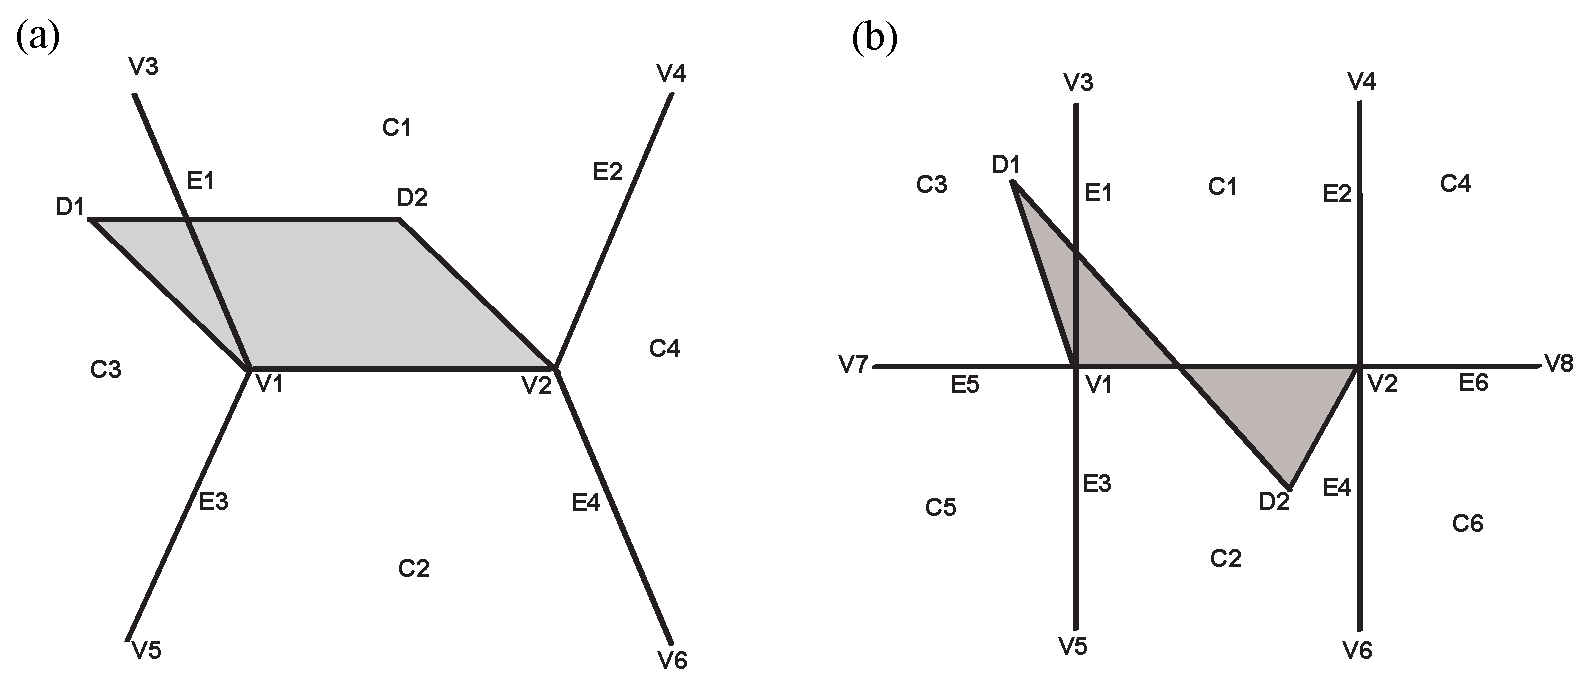
\includegraphics[width=1.0\textwidth]{seaice/ir_diagram.eps}
\caption{(a): Schematic showing transport across a cell edge on a standard MPAS mesh with 3 edges meeting at each vertex. The letters $C$, $E$ and $V$ denote cell centers, edges and vertices, respectively. Points $D1$ and $D2$ are backward trajectories, and the departure region is shaded. (b): Schematic showing transport across a cell edge on a quadrilateral MPAS mesh with 4 edges meeting at each vertex.}
\label{fig:IR_geom}
\end{figure}

The edges and vertices in Figure~\ref{fig:IR_geom}a are defined in a coordinate system lying in the local tangent plane at the midpoint of the main edge, halfway between $V1$ and $V2$. These coordinates are pre-computed at initialization. During each time step, departure triangles are found by locating $D1$ and $D2$ in this coordinate system, and then looping through the edges to identify any intersections of line segment $\overline{D12}$ (i.e., the segment joining $D1$ and $D2$) with the various edges. If $\overline{D12}$ intersects the main edge, then the departure region consists of two triangles (one each in $C1$ and $C2$) rather than a quadrilateral (as shown in the figure). If $\overline{D12}$ intersects any of edges $E1$ to $E4$, the departure region includes triangles in side cells.

Each departure triangle lies in a single grid cell, and there are at most four such triangles. There are two triangles in the central cells (either one each in $C1$ and $C2$, or a quadrilateral that can be split into two triangles), and up to two triangles in side cells. The triangle vertices are a combination of cell vertices ($V1$ and $V2$), departure points ($D1$ and $D2$), and intersection points (points where $\overline{D12}$ crosses an edge).

Figure~\ref{fig:IR_geom}b shows the geometry for a quadrilateral mesh. In this figure the departure region consists of two triangles, but it could also be a quadrilateral as in Figure~\ref{fig:IR_geom}a. For the quad mesh there are two additional side cells ($C5$ and $C6$), edges ($E5$ and $E6$) and vertices ($V7$ and $V8$). The search algorithm is designed such that the code used to find departure triangles for the standard mesh is also  applied to the quad mesh. For quad meshes only, there is additional logic to find intersection points and triangles associated with the extra edges and cells. This is the only mesh-specific code in the run-time IR code. For the quad mesh there are at most six departure triangles: two in the central cells and one in each of the four side cells. If the edges meet at right angles as shown in the figure, the maximum is five triangles, but this is not a mesh requirement.

Once triangle vertices have been found in edge-based coordinates, they are transformed to cell-based coordinates, i.e., coordinates in the local tangent plane of the cell containing each triangle. (Coefficients for these transformations are computed at initialization.) Triangle areas are computed as 
\begin{equation}
\label{eq:triangle_area}
{{A}_{T}}=\frac{1}{2}\left| ({{x}_{2}}-{{x}_{1}})({{y}_{3}}-{{y}_{1}})-({{y}_{2}}-{{y}_{1}})({{x}_{3}}-{{x}_{1}}) \right|.
\end{equation}

\subsubsection{Integrating the transport}
\label{IR_integrate}

Next, ice area and area-tracer products are integrated in each triangle. The integrals have the form (\ref{eq:recover_a}) for area and (\ref{eq:recover_T}) for tracers. Since each field is a linear function of $(x,y)$ as in (\ref{eq:reconstruct_a}) and (\ref{eq:reconstruct_T}), the area-tracer products are quadratic, cubic and quartic polynomials, respectively, for tracers of type 1, 2 and 3.

The integrals can be evaluated exactly by summing over values at quadrature points in each triangle. Polynomials of quadratic or lower order are integrated using the formula
\begin{equation}
\label{eq:quadrature1}
I = \frac{{{A}_{T}}}{3}\sum\limits_{i=1}^{3}{f({{{\mathbf{{x}'}}}_{i}})}.
\end{equation}
The quadrature points are located at ${{\mathbf{{x}'}}_{i}}=({{\mathbf{x}}_{0}}+{{\mathbf{x}}_{i}})/2$, where $\mathbf{x_0}$ is the triangle midpoint and $\mathbf{x_i}$ are the three vertices. The products involving type-2 and type-3 tracers are cubic and quadratic polynomials, which can be evaluated using a similar formula with 6 quadrature points:
\begin{equation}
\label{eq:quadrature2}
I = {{A}_{T}}\left[ {{w}_{1}}\sum\limits_{i=1}^{3}{f({{\mathbf{x}}_{1i}})}+{{w}_{2}}\sum\limits_{i=1}^{3}{f({{\mathbf{x}}_{2i}})} \right],
\end{equation}
where $\mathbf{x_{1i}}$ and $\mathbf{x_{2i}}$ are two sets of three quadrature points, arranged symmetrically on trisecting medians of the triangle, and $w_1$ and $w_2$ are weighting factors. Coefficients and weighting factors for these and other symmetric quadrature rules for triangles were computed by \citet{Dunavant85}. These integrals are computed for each triangle and summed over edges to give fluxes of ice area and area-tracer products across each edge.

\subsubsection{Updating area and tracer fields}
\label{IR_update}

The area transported across edge $k$ for a given cell can be denoted as $\Delta a_k$,  and the area-tracer products as $\Delta (a T_1)_k$, $\Delta (a T_1 T_2)_k$ and $\Delta (a T_1 T_2 T_3)_k$. The new ice area at time $n+1$ is given by
\begin{equation}
\label{eq:update_a}
{{a}^{n+1}} = {{a}^{n}}+\frac{1}{{{A}_{C}}}\sum\limits_{k}{\pm \Delta {{a}_{k}}},
\end{equation}
where the sum is taken over cell edges $k$, with a positive sign denoting transport into a cell and a negative sign denoting outward transport. The new tracers are given by
\begin{align}
\begin{split}
\label{eq:update_T}
   T_{1}^{n+1} & = \frac{{{a}^{n}}T_{1}^{n}+\frac{1}{{{A}_{C}}}\sum\limits_{k}{\pm \Delta {{(a{{T}_{1}})}_{k}}}}{{{a}^{n+1}}},  \\
   T_{2}^{n+1} & = \frac{{{a}^{n}}T_{1}^{n}T_{2}^{n}+\frac{1}{{{A}_{C}}}\sum\limits_{k}{\pm \Delta {{(a{{T}_{1}}{{T}_{2}})}_{k}}}}{{{a}^{n+1}}T_{1}^{n+1}},  \\
   T_{3}^{n+1} & =\frac{{{a}^{n}}T_{1}^{n}T_{2}^{n}T_{3}^{n}+\frac{1}{{{A}_{C}}}\sum\limits_{k}{\pm \Delta {{(a{{T}_{1}}{{T}_{2}}{{T}_{3}})}_{k}}}}{{{a}^{n+1}}T_{1}^{n+1}T_{2}^{n+1}}.
\end{split}
\end{align}
\citet{Dukowicz00} showed that (\ref{eq:update_T}) satisfies tracer
monotonicity, since the new-time tracer values are area-weighted
averages of old-time values.


\section{Column Physics}
\label{sec:column_physics}

Namelist parameters for the \verb+forcing+ namelist group.


\chapter{Standalone Simulations}
\label{chap:standalone_simulations}

\section{Input Data}
\label{sec:input_data}

Input data for simple standalone simulations and for the MPAS-Seaice testing system are available at http://doi.org/10.5281/zenodo.1219191. The data consists of model domain grid files and forcing data for two different domains: a quasi-uniform 120 km resolution mesh, and a quasi-uniform 240 km resolution mesh. Included files for the quasi-uniform 120 km domain are:

\begin{table}[H]
\begin{tabular}{ll}
\hline
Filename & Description \\
\hline
\lstinline+LYq_monthly.nc+ & Monthly climatology atmospheric forcing file. \\
\lstinline+LYq_six_hourly.2000.nc+ & Six hourly Atmospheric forcing file. \\
\lstinline+culled_graph.info.part.16+ & Grid partition file for 16 processors. \\
\lstinline+culled_graph.info.part.32+ & Grid partition file for 32 processors. \\
\lstinline+get_domain.py+ & Script to set up MPAS-Seaice run directory. \\
\lstinline+mpas_seaice_domain_manifest+ & Contents of this directory. \\
\lstinline+oceanmixed_ice_depth_QU120km.nc+ & Ocean forcing file. \\
\lstinline+seaice_QU_120km.nc+ & Grid file for the quasi-uniform 120 km domain \\
\lstinline+snicar_optics_5bnd_mam_c140303_mpas_seaice.nc+ &  \\
\lstinline+standard_optics_mpas_seaice.nc+ &  \\
\hline
\end{tabular}
\end{table}
\section{Standard Configurations}
\label{sec:standard_configurations}

Several standard configurations (namelist and streams files) are available in the MPAS repository at \verb+MPAS/testing_and_setup/seaice/configurations/+. The \verb+standard_physics+ is the standard configuration for testing and exercises the standard physics configuration. All configurations:

\begin{table}[H]
\begin{tabular}{ll}
\hline
Configuration & Description \\
\hline
\lstinline+standard_physics+ & A standard physics configuration without BGC \\
\lstinline+standard_physics_single_cell+ & As \lstinline+standard_physics+ but with a single cell. \\
\lstinline+standard_bgc+ &  \\
\hline
\end{tabular}
\end{table}
\section{Quick start simulation}
\label{sec:simple_simulations}

Successful building of MPAS-Seaice (see chapter \ref{chap:mpas_build_instructions} for building instructions) can be demonstrated by running a simple simulation with the test data described in section \ref{sec:input_data}. To run the model with the quasi-uniform 120 km domain and the \lstinline+standard_physics+ configuration:

\begin{enumerate}

\item Create a run directory and execute the \lstinline+get_domain.py+ script from the \lstinline+domain_QU120km+ directory of the input data. This create symbolic links with the correct names to the grid and forcing data.

\item Copy the streams and namelist files from the \lstinline+standard_physics+ directory of the sea-ice configurations directory (see section \ref{sec:standard_configurations}) of the MPAS repository.

\item Execute the \lstinline+seaice_model+ MPAS-Seaice executable from the run directory. The model should run and generate a log file called \lstinline+log.seaice.0000.out+.

\end{enumerate}


\section{Testing}
\label{sec:testing}



% new chapters
\chapter[Namelist options]{\hyperref[chap:namelist_sections]{Namelist options}}
\label{chap:namelist_tables}
Embedded links point to more detailed namelist information in the appendix.
\section[velocity\_solver]{\hyperref[sec:nm_sec_velocity_solver]{velocity\_solver}}
\label{sec:nm_tab_velocity_solver}
\section{Velocity Solver}
\label{sec:velocity_solver}

\subsection{Overview}

MPAS-Seaice uses a `B' Arakawa type grid \citep{Arakawa77} with both components of velocity defined at cell vertices and sea-ice concentration, volume and other tracers defined at cell centers (see Chapter \ref{chap:mpas_grid_description}). When using CICE-like quadrilateral meshes, this allows the velocity solver algorithm of MPAS-Seaice to reduce to that of CICE, allowing CICE and MPAS-Seaice to use identical test cases and allow rapid testing and development. 

In CICE the velocity components are aligned with the quadrilateral mesh. This is not possible, in general, with MPAS-Seaice since a SCVT MPAS mesh does not have edges with perpendicular directions as in a quadrilateral mesh. Instead, the velocity components at a given MPAS vertex are defined as eastwards ($u$) and northwards ($v$), irrespective of the orientation of edges joining that vertex. Such a definition, however, would result in a convergence of $v$ components at the geographic North Pole and strong metric terms in the velocity solution. Consequently, in addition, we rotate these definitions of $u$ and $v$ so that their pole lies on the geographical equator at $0^\circ$ longitude. 

To prognose sea-ice velocity we solve the same sea-ice momentum equation as CICE \citep{Hibler79,Hunke97}:
\begin{equation}
m \frac{\partial{\boldsymbol{u}}}{\partial{t}} = \boldsymbol{\nabla} \cdot \boldsymbol{\sigma} + \boldsymbol{\tau_a} + \boldsymbol{\tau_w} - \boldsymbol{\hat{k}} \times m f \boldsymbol{u} -mg \boldsymbol{\nabla}H_o.
\end{equation}
Here $m$ is the mass of snow and ice per unit area, $\boldsymbol{u}$ is the sea-ice velocity, $\boldsymbol{\sigma}$ is the ice internal stress tensor, $\boldsymbol{\tau_a}$ and $\boldsymbol{\tau_w}$ are the horizontal stresses due to atmospheric winds and ocean currents respectively, $\boldsymbol{\hat{k}}$ is the unit vector normal to the Earth surface, $f$ is the Coriolis parameter, $g$ is the acceleration due to gravity and $H_o$ is the ocean surface height. The second to last term represents the Coriolis force and the last term represents the force due to the ocean surface tilt. Only the divergence of internal stress and ocean surface tilt terms depend on horizontal differential operators. During coupled simulations the ocean model provides the ocean surface tilt term, whereas in non-coupled simulations we assume that the ocean currents are in geostrophic balance so that
\begin{equation}
mg \boldsymbol{\nabla}H_o = m f \boldsymbol{\hat{k}} \times \boldsymbol{u_o}
\end{equation}
where $\boldsymbol{u_o}$ is the ocean surface velocity. Consequently, only the divergence of internal stress depends on the properties of the horizontal grid employed, and only adaptations to this stress term are required to adapt the velocity solver of CICE to MPAS meshes. The other terms in the momentum equation are solved in an identical way to CICE.

Determination of the divergence of the internal stress can be broken down into three stages: 
\begin{enumerate}
\item The strain rate tensor is determined from the velocity field.
\item The stress tensor at a point is determined, through a constitutive relation, from the strain rate tensor at that point.
\item The divergence of this stress tensor is calculated. 
\end{enumerate}
As in CICE we use an Elastic-Viscous-Plastic (EVP) rheology \citep{Hunke97} for the constitutive relation. This step does not depend on the details of the horizontal mesh and we use the same formulation as CICE. We develop two schemes to calculate the strain rate tensor and the divergence of internal stress on MPAS meshes. A variational scheme is based on that used in CICE \citep{Hunke02}, whereas a weak scheme uses the line integral forms of the symmetric gradient and divergence operators. These schemes are described in the following sections.

\subsection{Variational Scheme}

We develop a variational scheme for calculating the divergence of stress based on that of \citet{Hunke02} but adapted for arbitrarily shaped and sided convex polygons. This scheme is based on the fact that over the entire domain, $\Omega$, and ignoring boundary effects, the total work done by the internal stress is equal to the dissipation of mechanical energy:
\begin{equation}
\int_\Omega \boldsymbol{u} \cdot (\boldsymbol{\nabla} \cdot \boldsymbol{\sigma}) \mathrm{d}A = -\int_\Omega (\boldsymbol{\sigma_{11}} \boldsymbol{\dot{\epsilon}_{11}}  + 2 \boldsymbol{\sigma_{12}} \boldsymbol{\dot{\epsilon}_{12}} + \boldsymbol{\sigma_{22}} \boldsymbol{\dot{\epsilon}_{22}}) \mathrm{d}A.
\label{eqn:work_done}
\end{equation}
Here $\boldsymbol{\dot{\epsilon}}$ is the strain rate tensor and the integrals are area integrals over the whole model domain. The work done over the whole domain can be split into a sum over the contribution to the work done from each cell on the dual Delaunay mesh. Each dual cell on the dual mesh consists of a triangle surrounding a single vertex point where the discretized velocity is defined. Equation \ref{eqn:work_done} can then be written as
\begin{equation}
\sum_i^{n_d} \int_i \boldsymbol{u} \cdot (\boldsymbol{\nabla} \cdot \boldsymbol{\sigma}) \mathrm{d}A = D(u_1, u_2, ..., u_n, v_1, v_2, ..., v_{n_d})
\end{equation}
where the left-side sum is over the $n_d$ cells of the dual mesh, the integral is an area integral over each dual cell,  and the dissipation of mechanical energy has been written as a function of the discretized velocity components.
Writing the two components of the divergence of stress as $F_u=(\nabla \cdot \sigma)_u$ and $F_v=(\nabla \cdot \sigma)_v$, then
\begin{equation}
\sum_i^{n_d} \int_i (uF_u + vF_v) \mathrm{d}A = D(u_1, u_2, ..., u_n, v_1, v_2, ..., v_{n_d}).
\end{equation}
If we assume that within the dual cell the velocity is constant, it follows that
\begin{equation}
\sum_i^{n_d} (u_i F_{ui} + v_i F_{vi}) A_{ui} = D(u_1, u_2, ..., u_n, v_1, v_2, ..., v_{n_d})
\end{equation}
where $A_{ui}$ is the area of the dual mesh cell.
The variation of these expressions with respect to the $u$ component of the discretized velocity at a particular vertex point $j$ is given by
\begin{equation}
\frac{\partial{}}{\partial{u_j}} \sum_i^{n_d} (u_i F_{ui} + v_i F_{vi}) A_{ui} =  \frac{\partial{}}{\partial{u_j}}D(u_1, u_2, ..., u_n, v_1, v_2, ..., v_{n_d})
\end{equation}
Assuming $F_u$ and $F_v$ are not functions of velocity,
\begin{equation}
F_{uj} =  \frac{1}{A_{uj}} \frac{\partial{}}{\partial{u_j}}D(u_1, u_2, ..., u_n, v_1, v_2, ..., v_{n_d}).
\label{eqn:variation}
\end{equation}
$F_v$ is obtained in a similar way by taking the variation of $D$ with respect to $v_j$. The dissipation of mechanical energy, $D$, can be split into three terms: 
\begin{equation}
D=D_1+ D_2+D_3
\end{equation}
with
\begin{equation}
D_1=-\int  \boldsymbol{\sigma_{11}} \boldsymbol{\dot{\epsilon}_{11}} \mathrm{d}A ,\quad D_2=-\int  2 \boldsymbol{\sigma_{12}} \boldsymbol{\dot{\epsilon}_{12}} \mathrm{d}A, \quad D_3=-\int  \boldsymbol{\sigma_{22}} \boldsymbol{\dot{\epsilon}_{22}} \mathrm{d}A.
\end{equation}
We will calculate the contribution to $F_u$ and $F_v$ from $D_1$. Similar contributions come from $D_2$ and $D_3$. Using the expression for $\dot{\epsilon}_{11}$ in terms of the velocity components and latitude $\phi$, $D_1$ becomes
\begin{equation}
D_1=-\int  \sigma_{11} \left[ \frac{\partial{u}}{\partial{x}} - \frac{v \tan{\phi}}{r} \right] \mathrm{d}A
\end{equation}
where $x$ and $y$ are locally Cartesian coordinates, with $x$ in the rotated due eastwards direction and $y$ in the rotated due northwards direction, $\phi$ is the latitude, and $r$ is the radius of the Earth. The second term in $\dot{\epsilon}$ accounts for the metric effects of the curved domain \citep{Batchelor67}.
The integral can be broken up into a sum over the $n_p$ cells in the primary mesh:
\begin{equation}
D_1=- \sum_k^{n_p} \int_k  \sigma_{11} \left[ \frac{\partial{u}}{\partial{x}} - \frac{v \tan{\phi}}{r} \right] \mathrm{d}A
\label{eqn:d_1}
\end{equation}
where the integral is over the interior area of the $k$th cell. 
To perform this integral we use a set of basis functions, $\mathcal{W}_l$, to represent functions within a cell of the primary mesh. If a function, $\psi$, has a value of  $\psi_l$ at vertex $l$ of a cell, then the value of the function at a position $(x,y)$ within the cell can be approximated as
\begin{equation}
\psi(x,y) = \sum_l^{n_v} \psi_l \mathcal{W}_l (x,y)
\end{equation}
where the sum is over the $n_v$ vertices of the cell in the primary mesh.
Using those basis functions, equation \ref{eqn:d_1} can be written as 
\begin{equation}
D_1=-\sum_k^{n_p} \int_k \left[ \sum_{l}^{n_v} \sigma_{11{l}} \mathcal{W}_{l} \cdot \sum_{m}^{n_v} \left(u_{m} \frac{\partial{\mathcal{W}_{m}}}{\partial{x}} - \frac{\tan{\phi}}{r} v_{m} \mathcal{W}_{m} \right) \right]\mathrm{d}A
\end{equation}
where the derivative with respect to $x$ has been taken inside the summation.
Rearranging
\begin{equation}
D_1= -\sum_k^{n_p} \sum_{l}^{n_v} \sum_{m}^{n_v} \sigma_{11{l}}\left( u_{m} \int_k  \mathcal{W}_{l}   \frac{\partial{\mathcal{W}_{m}}}{\partial{x}}  \mathrm{d}A  - \frac{\tan{\phi}}{r}  v_{m} \int_k \mathcal{W}_{l} \mathcal{W}_{m}  \mathrm{d}A  \right).
\end{equation}
In moving the integral, we have assumed that $\phi$, the latitude, is constant in the cell. The terms involving integrals are now only a function of the geometry of the mesh and can be calculated once during the initialization phase of the model run. Defining 
\begin{equation}
\mathcal{S}^x_{lm} = \int_k  \mathcal{W}_{l}   \frac{\partial{\mathcal{W}_{m}}}{\partial{x}}  \mathrm{d}A
\end{equation}
and
\begin{equation}
\mathcal{T}_{lm} = \int_k \mathcal{W}_{l} \mathcal{W}_{m}  \mathrm{d}A.
\end{equation}
we have
\begin{equation}
D_1= -\sum_k^{n_p} \sum_{l}^{n_v} \sum_{m}^{n_v} \sigma_{11{l}}\left( u_{m} \mathcal{S}^x_{lm}  - \frac{\tan{\phi}}{r}  v_{m} \mathcal{T}_{lm}  \right).
\end{equation}
Taking the variation with respect to a discretized velocity component at a particular vertex point, $j$, as in equation \ref{eqn:variation}, now gives us the contribution from $D_1$ to the components of the divergence of stress tensor at that velocity point:
\begin{equation}
(\nabla \cdot \sigma)_{u_j}^{D_1} = \frac{\delta D_1}{\delta u_{j}}= -\sum_k^{n_p} \sum_{l}^{n_v}  \sigma_{11{l}} \mathcal{S}^x_{lj}
\end{equation}
\begin{equation}
(\nabla \cdot \sigma)_{v_j}^{D_1} = \frac{\delta D_1}{\delta v_{j}}= \sum_k^{n_p} \sum_{l}^{n_v}  \sigma_{11{l}}  \frac{\tan{\phi}}{r} \mathcal{T}_{lj}
\end{equation}
Only cells that border the vertex point $j$ contribute to the $k$ sum over cells. The total divergence of stress at the point $j$ is then the sum from the contributions from $D_1$, $D_2$, and $D_3$:
\begin{equation}
(\nabla \cdot \sigma)_{u_j} = (\nabla \cdot \sigma)_{u_j}^{D_1} + (\nabla \cdot \sigma)_{u_j}^{D_2} + (\nabla \cdot \sigma)_{u_j}^{D_3}
\end{equation}
\begin{equation}
(\nabla \cdot \sigma)_{v_j} = (\nabla \cdot \sigma)_{v_j}^{D_1} + (\nabla \cdot \sigma)_{v_j}^{D_2} + (\nabla \cdot \sigma)_{v_j}^{D_3}.
\end{equation}
All that remains now is to determine the stress for each cell at its vertices. As in the formulation in CICE, each cell has its own values of the stress at its vertices, so each vertex has several values of the stress, each corresponding to a different surrounding cell. The stresses are calculated from the strain rate tensor at each vertex using the constitutive relation. Including metric effects \citep{Batchelor67} the strain rate tensor is given by:
\begin{equation}
\dot{\epsilon}_{11} = \frac{\partial{u}}{\partial{x}} - \frac{v \tan{\phi}}{r}
\end{equation}
\begin{equation}
\dot{\epsilon}_{22} = \frac{\partial{v}}{\partial{y}}
\end{equation}
\begin{equation}
\dot{\epsilon}_{12} = \frac{1}{2} \left( \frac{\partial{u}}{\partial{y}} + \frac{\partial{v}}{\partial{x}} \right) + \frac{u \tan{\phi}}{2 r}.
\end{equation}
The strain rate tensor at cell vertex $l$ is then given by 
\begin{equation}
\dot{\epsilon}_{11{l}} =  \sum_{m}^{n_v} u_{m} \left. \frac{\partial{\mathcal{W}_{m}}}{\partial{x}} \right| _{l} - \frac{v_{l} \tan{\phi_{l}}}{r}
\end{equation}
\begin{equation}
\dot{\epsilon}_{22{l}} =  \sum_{m}^{n_v} v_{m} \left. \frac{\partial{\mathcal{W}_{m}}}{\partial{y}} \right| _{l} 
\end{equation}
\begin{equation}
\dot{\epsilon}_{12{l}} = \frac{1}{2} \left( \sum_{m}^{n_v} u_{m} \left. \frac{\partial{\mathcal{W}_{m}}}{\partial{y}} \right| _{l} +\sum_{m}^{n_v} v_{m} \left. \frac{\partial{\mathcal{W}_{m}}}{\partial{x}} \right| _{l}  \right) + \frac{u_{l} \tan{\phi_{l}}}{2 r}
\end{equation}
The derivatives of the basis functions are taken at cell vertex $l$.

In MPAS-Seaice we provide two options for the choice of basis functions, $\mathcal{W}_l$: Wachspress basis functions and Piece-Wise Linear (PWL) basis functions. Both basis functions have a value of one on vertex $l$ and zero on the other vertices of a cell, and are linear on the cell boundaries. The Wachspress basis functions are smooth rational polynomials in the cell interior \citep{Dasgupta03}. The integrals of the Wachspress basis function within a cell are performed using the eighth order quadrature rules of \citet{Dunavant85}. PWL basis functions divide the polygonal cell into sub-triangles and use a linear basis within each sub-triangle \citep{Bailey08}. To divide the polygonal cell into sub-triangles, a point is chosen within the cell and sub-triangles formed using this point and two adjacent vertices. The central point in the cell, $\mathbf{x}_c$,  is chosen as
\begin{equation}
\mathbf{x}_c = \sum_i^{n_v} \alpha_i \mathbf{x}_i
\end{equation}
where the sum is over the $n_v$ vertices of the cell each with position $\mathbf{x}_i$. The simplest choice for the $\alpha_i$ is to set them all equal to the inverse of the number of cell vertices, $1/n_v$. For quadrilateral meshes the Wachspress basis functions reduce to the bilinear basis functions used in CICE.

\subsection{Weak Scheme}

\begin{figure}[]
\centering
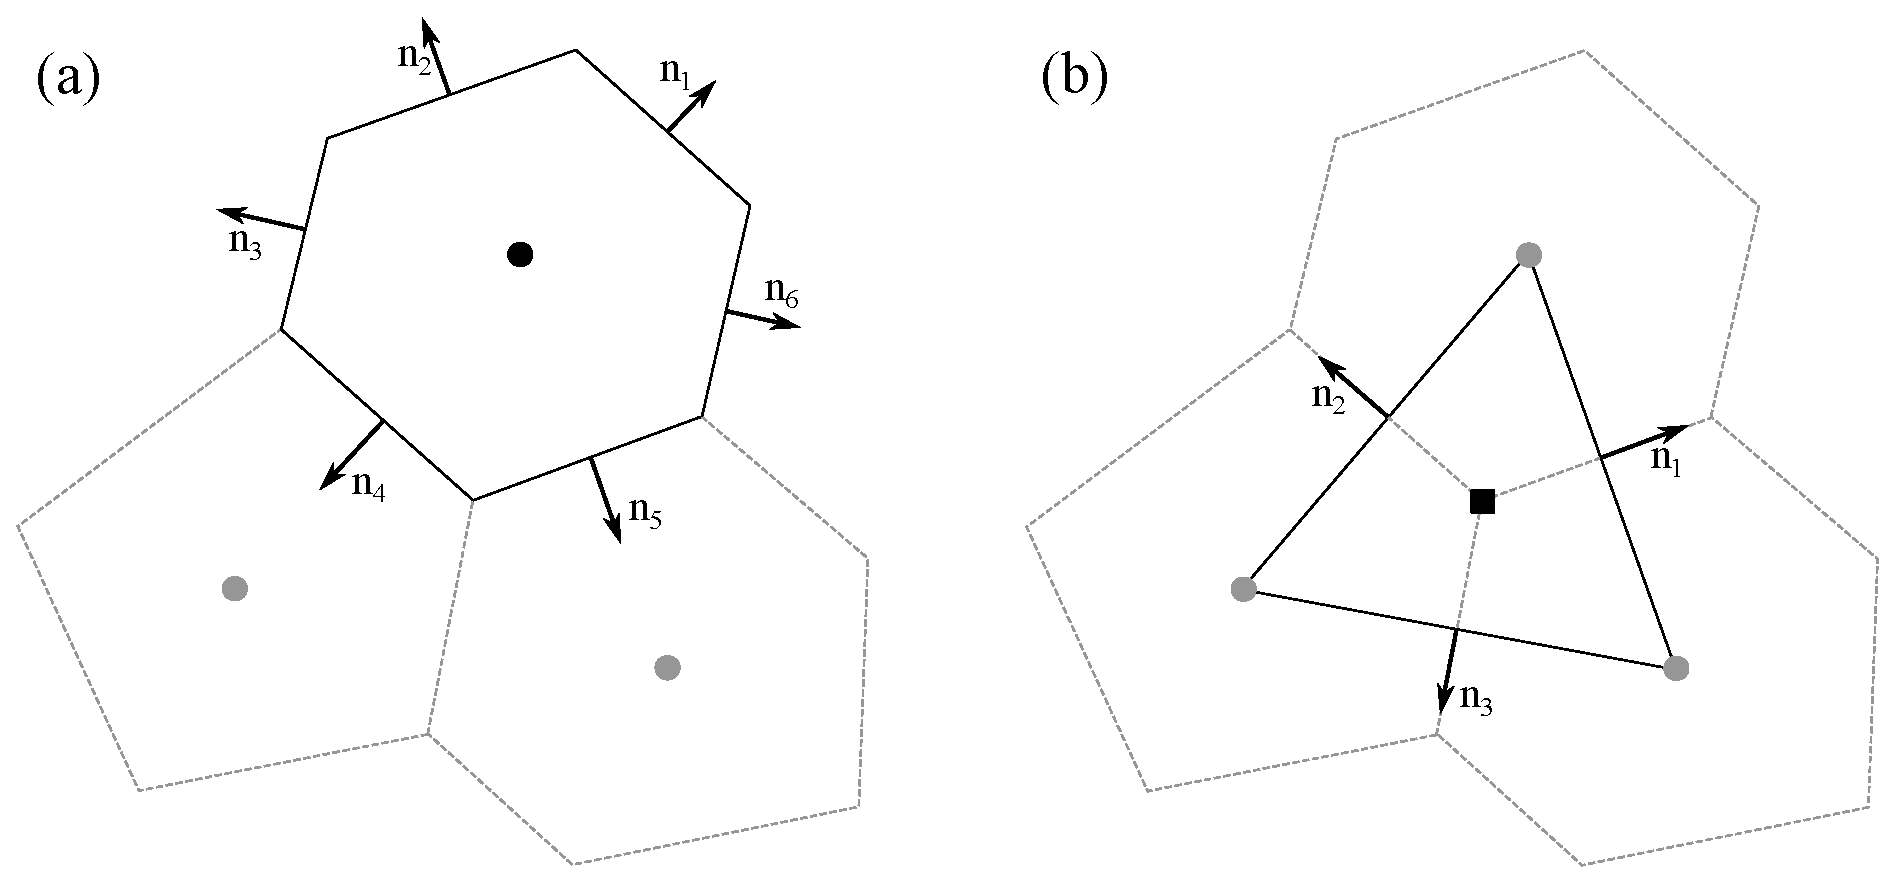
\includegraphics[width=\linewidth]{seaice/figures/mesh_weak.eps}
\caption{Contour integration lines used by the weak scheme. (a): Strain rate at cell centers (\emph{circle}) are calculated from line integrals around primary mesh cells (\emph{solid line}). (b): Divergence of stress at cell vertices (\emph{square}) are calculated from line integrals around the dual mesh cells (\emph{solid line}). Directions of normal vectors used in the integrals are shown for both figures.}
\label{fig:mesh_weak}
\end{figure}

For the weak scheme we use line integrals around cells in the primary and dual meshes to calculate the strain rate tensor and the divergence of stress, respectively. To determine the strain rate tensor we start from the following vector identity:
\begin{equation}
\boldsymbol{\nabla} \cdot (\boldsymbol{u} \otimes \boldsymbol{v}) = (\boldsymbol{u} \cdot \boldsymbol{\nabla}) \boldsymbol{v} + (\boldsymbol{\nabla} \cdot \boldsymbol{u}) \boldsymbol{v}
\label{eqn:vector_identity}
\end{equation}
and from the divergence theorem:
\begin{equation}
\int_\Omega \left[ \boldsymbol{\nabla} \cdot (\boldsymbol{u} \otimes \boldsymbol{v}) \right] \partial{\Omega} = \oint_S \left[\boldsymbol{n} \cdot (\boldsymbol{u} \otimes \boldsymbol{v}) \right] \partial{S} = \oint_S \left[(\boldsymbol{n} \cdot \boldsymbol{u}) \boldsymbol{v} \right] \partial{S}
\label{eqn:divergence_theorem}
\end{equation}
where $\boldsymbol{n}$ is a normal vector to the surface $S$ and $\otimes$ is the tensor product.
If equation \ref{eqn:vector_identity} is integrated over $\Omega$, using equation \ref{eqn:divergence_theorem} we obtain
\begin{equation}
\int_\Omega \left[ (\boldsymbol{u} \cdot \boldsymbol{\nabla}) \boldsymbol{v} + (\boldsymbol{\nabla} \cdot \boldsymbol{u}) \boldsymbol{v} \right] \partial{\Omega} = \oint_S \left[(\boldsymbol{n} \cdot \boldsymbol{u}) \boldsymbol{v} \right] \partial{S}
\label{eqn:weak1}
\end{equation}
If $\boldsymbol{u}$ is chosen as constant then $\boldsymbol{\nabla} \cdot \boldsymbol{u}$ vanishes as does the second term in equation \ref{eqn:weak1}. Taking, also, $\boldsymbol{u}$ sequentially as the cartesian unit vectors spanning $\Omega$ and summing the results we obtain
\begin{equation}
\int_\Omega \left[ \boldsymbol{\nabla} \boldsymbol{v} \right] \partial{\Omega} = \oint_S \left[ \boldsymbol{n} \otimes \boldsymbol{v} \right] \partial{S}
\end{equation}
The symmetric version of this operator is then obtained as:
\begin{equation}
\int_\Omega \left[ \boldsymbol{\nabla_S} \boldsymbol{v} \right] \partial{\Omega} = \oint_S \left[ \boldsymbol{n} \otimes \boldsymbol{v} + \boldsymbol{v} \otimes \boldsymbol{n} \right] \partial{S}
\end{equation}
The strain rate at a point is then obtained from the limit
\begin{equation}
\boldsymbol{\dot{\epsilon}} = \boldsymbol{\nabla}_S \boldsymbol{v} = \lim_{A \to 0} \frac{1}{A} \oint \frac{1}{2}\left[ \boldsymbol{n} \otimes \boldsymbol{v} + \boldsymbol{v} \otimes \boldsymbol{n} \right] \mathrm{d}l
\end{equation}
where the integral is around a closed loop with area $A$ and normal vector $\boldsymbol{n}$, and $\boldsymbol{v}$ is the sea-ice velocity.
To determine the strain rate tensor at the centers of the primary mesh, we take this integration around the edges of the cells in the primary mesh. First the cell is projected onto a flat tangent plane perpendicular to the vector joining the center of the sphere to the cell center. We take the sea ice velocity at a cell edge as the average of the values on the two vertices forming that edge projected onto the tangent plane:
\begin{equation}
\boldsymbol{\dot{\epsilon}}^\prime = \frac{1}{A} \sum_i^{n_e} \frac{1}{2} \left[ \boldsymbol{n}_i \otimes \boldsymbol{v}_i + \boldsymbol{v}_i \otimes \boldsymbol{n}_i \right] l_i
\end{equation}
Here, $A$ is the area of the primary cell, the summation is over the $n_e$ edges of the primary cell, $\boldsymbol{n}_i$ is the normal vector to the edge $i$ that lies in the tangent plane, $\boldsymbol{v}_i$ is the edge velocity and $l_i$ is the length of edge $i$. We use the tangental projection of the velocity and account for metric terms separately. The full strain rate tensor including these metric terms is \citep{Batchelor67}:
\begin{equation}
\dot{\epsilon}_{11} = \dot{\epsilon}_{11}^\prime - \frac{v \tan{\phi}}{r}
\end{equation}
\begin{equation}
\dot{\epsilon}_{22} = \dot{\epsilon}_{22}^\prime
\end{equation}
\begin{equation}
\dot{\epsilon}_{12} = \dot{\epsilon}_{12}^\prime + \frac{u \tan{\phi}}{2r}
\end{equation}
where the prime symbol signifies a strain rate without metric terms.
The stress, which is determined from the strain rate tensor using the constitutive relation, is now defined on cell centers. To find its divergence we use the divergence theorem:
\begin{equation}
\iint \boldsymbol{\nabla} \cdot \boldsymbol{\sigma} \mathrm{d}A = \oint \left[ \boldsymbol{\sigma} \cdot \boldsymbol{n} \right] \mathrm{d}l
\end{equation}
or
\begin{equation}
\boldsymbol{\nabla} \cdot \boldsymbol{\sigma} = \lim_{A \to 0}  \frac{1}{A} \oint \left[ \boldsymbol{\sigma} \cdot \boldsymbol{n} \right] \mathrm{d}l
\end{equation}
for the divergence of stress at a point.
The divergence of internal stress is determined at primary cell vertices (where the velocity is defined and momentum equation solved) by performing a sum around the edges of the dual mesh on a tangent projected plane, tangental to the primary cell vertex. The vertices of the dual mesh are the cell centers of the primary mesh where the strain rate has been determined. The divergence of stress at primary cell vertices is then given by
\begin{equation}
(\boldsymbol{\nabla} \cdot \boldsymbol{\sigma})^\prime = \frac{1}{A_d} \sum_i^{n_c} \left[ \boldsymbol{\sigma}_i \cdot \boldsymbol{n}_i \right] l_i
\end{equation}
where $A_d$ is the area of the dual mesh cell, the sum is over the $n_c$ vertices of the dual mesh, $l_i$ is the length of the $i$ edge of the dual mesh, and $n_i$ is a normal vector to the $i$ edge on the projected plane. As before, this gives a result without taking into account metric effects of the mesh. With those effects the divergence of stress is:
\begin{equation}
(\nabla \cdot \sigma)_u = (\nabla \cdot \sigma)_u^\prime - \frac{2 \sigma_{12} \tan{\phi}}{r}
\end{equation}
\begin{equation}
(\nabla \cdot \sigma)_v = (\nabla \cdot \sigma)_v^\prime + \frac{(\sigma_{11} + \sigma_{22}) \tan{\phi}}{r}
\end{equation}
where the components of $\boldsymbol{\sigma}$ are approximated as the
average of the values on the dual mesh vertices.

\vspace{0.5in}
{\small
\begin{center}
\begin{longtable}{| p{2.0in} || p{4.0in} |}
    \hline
    {\bf Name} & {\bf Description} \endfirsthead
    \hline 
    {\bf Name} & {\bf Description} (Continued) \endhead
    \hline
    \hline
    \hyperref[subsec:nm_sec_config_velocity_solver]{config\_velocity\_solver} & Selection of the method for solving ice velocity. 'L1L2', 'FO', and 'Stokes' require compiling with external dycores. 'none' skips the calculation of velocity so the velocity field will be 0 or set to a field read from an input file.  'simple' gives a simple prescribed velocity field computed at initialization. \\
    \hline
    \hyperref[subsec:nm_sec_config_sia_tangent_slope_calculation]{config\_sia\_tangent\_slope\_\-calculation} & Selection of the method for calculating the tangent component of surface slope at edges needed by the SIA velocity solver. 'from\_vertex\_barycentric' interpolates upperSurface values from cell centers to vertices using the barycentric interpolation routine in operators (mpas\_cells\_to\_points\_using\_baryweights) and then calculates the slope between vertices.  It works for obtuse triangles, but will not work correctly across the edges of periodic meshes. 'from\_vertex\_barycentric\_kiteareas' interpolates upperSurface values from cell centers to vertices using barycentric interpolation based on kiterea values and then calculates the slope between vertices.  It will work across the edges of periodic meshes, but will not work correctly for obtuse triangles. 'from\_normal\_slope' uses the vector operator mpas\_tangential\_vector\_1d to calculate the tangent slopes from the normal slopes on the edges of the adjacent cells.  It will work for any mesh configuration, but is the least accurate method. \\
    \hline
    \hyperref[subsec:nm_sec_config_flowParamA_calculation]{config\_flowParamA\_calculation} & Selection of the method for calculating the flow law parameter A.  If 'constant' is selected, the value is set to config\_default\_flowParamA.  The other options are calculated from the temperature field.  This calculation only applies if config\_velocity\_solver is set to 'sia'.  For the 'FO' velocity solver, this is set in the albany\_input.xml file. \\
    \hline
    \hyperref[subsec:nm_sec_config_do_velocity_reconstruction_for_external_dycore]{config\_do\_velocity\_\-reconstruction\_for\_external\_\-dycore} & By default, external, higher-order dycores return the uReconstructX and uReconstructY fields (which are the native locations of their FEM solution).  If this option is set to .true., uReconstructX and uReconstructY will be calculated by MPAS using framework's vector reconstruction routines based on the values of normalVelocity supplied by the external dycore.  This provides a way to test the calculation of normalVelocity in the interface. \\
    \hline
    \hyperref[subsec:nm_sec_config_simple_velocity_type]{config\_simple\_velocity\_type} & Selection of the type of simple velocity field computed at initialization when config\_velocity\_solver = 'simple'.  See mode\_forward/mpas\_li\_velocity\_simple.F for details of what the options do. \\
    \hline
    \hyperref[subsec:nm_sec_config_use_glp]{config\_use\_glp} & If true, then apply Albany's grounding line parameterization \\
    \hline
    \hyperref[subsec:nm_sec_config_beta_use_effective_pressure]{config\_beta\_use\_effective\_\-pressure} & If true, then multiply beta by effective pressure before passing to Albany.  This allows, e.g., a Weertman basal friction law with an effective pressure term.  Note that basal friction still needs to be selected in Albany xml file. \\
    \hline
\end{longtable}
\end{center}
}
\section[advection]{\hyperref[sec:nm_sec_advection]{advection}}
\label{sec:nm_tab_advection}
The advection namelist record controls options assocated with advection of thickness and tracers.  Tracer advection is not currently supported.

\vspace{0.5in}
{\small
\begin{center}
\begin{longtable}{| p{2.0in} || p{4.0in} |}
    \hline
    {\bf Name} & {\bf Description} \endfirsthead
    \hline 
    {\bf Name} & {\bf Description} (Continued) \endhead
    \hline
    \hline
    \hyperref[subsec:nm_sec_config_thickness_advection]{config\_thickness\_advection} & Selection of the method for advecting thickness ('fo' = first-order upwinding). \\
    \hline
    \hyperref[subsec:nm_sec_config_tracer_advection]{config\_tracer\_advection} & Selection of the method for advecting tracers. \\
    \hline
\end{longtable}
\end{center}
}
\section[calving]{\hyperref[sec:nm_sec_calving]{calving}}
\label{sec:nm_tab_calving}
The calving namelist record controls options assocated with calving of floating ice.

\vspace{0.5in}
{\small
\begin{center}
\begin{longtable}{| p{2.0in} || p{4.0in} |}
    \hline
    {\bf Name} & {\bf Description} \endfirsthead
    \hline 
    {\bf Name} & {\bf Description} (Continued) \endhead
    \hline
    \hline
    \hyperref[subsec:nm_sec_config_calving]{config\_calving} & Selection of the method for calving ice (as defined further below). \\
    \hline
    \hyperref[subsec:nm_sec_config_calving_topography]{config\_calving\_topography} & Defines the topographic height below which ice calves (for topographic\_threshold option). \\
    \hline
    \hyperref[subsec:nm_sec_config_calving_thickness]{config\_calving\_thickness} & Defines the ice thickness below which ice calves (for thickness\_threshold option). \\
    \hline
    \hyperref[subsec:nm_sec_config_calving_eigencalving_parameter_source]{config\_calving\_eigencalving\_\-parameter\_source} & Source of the eigencalving parameter value \\
    \hline
    \hyperref[subsec:nm_sec_config_calving_eigencalving_parameter_scalar_value]{config\_calving\_eigencalving\_\-parameter\_scalar\_value} & Value of eigencalving parameter if taken as a scalar by option config\_calving\_eigencalving\_parameter\_source. (Default value is 1.0e9 m a converted to units used here.) \\
    \hline
    \hyperref[subsec:nm_sec_config_data_calving]{config\_data\_calving} & Select whether or not to configure calving in a 'data' model mode (calc. calving flux but do not update ice geometry) \\
    \hline
    \hyperref[subsec:nm_sec_config_calving_timescale]{config\_calving\_timescale} & Defines the timescale for calving. The fraction of eligible ice that calves is min(dt/calving\_timescale, 1.0). A value of 0 means that all eligible ice calves. \\
    \hline
    \hyperref[subsec:nm_sec_config_restore_calving_front]{config\_restore\_calving\_front} & If true, then restore the calving front to its initial position.  If ice grows beyond the initial extent, it is removed.  If ice shrinks to an extent behind the initial extent, those locations are filled with thin ice (defined as 1/10th the value of config\_dynamic\_thickness).  Note that this violates conservation of mass and energy. \\
    \hline
\end{longtable}
\end{center}
}
\section[thermal\_solver]{\hyperref[sec:nm_sec_thermal_solver]{thermal\_solver}}
\label{sec:nm_tab_thermal_solver}
The thermal\_solver namelist record controls options assocated with temperature evolution.

\vspace{0.5in}
{\small
\begin{center}
\begin{longtable}{| p{2.0in} || p{4.0in} |}
    \hline
    {\bf Name} & {\bf Description} \endfirsthead
    \hline 
    {\bf Name} & {\bf Description} (Continued) \endhead
    \hline
    \hline
    \hyperref[subsec:nm_sec_config_thermal_solver]{config\_thermal\_solver} & Selection of the method for the vertical thermal solver (possible values are described further below). \\
    \hline
    \hyperref[subsec:nm_sec_config_thermal_calculate_bmb]{config\_thermal\_calculate\_bmb} & Determines if basal and internal melting calculated by the thermal solver should contribute to basal mass balance or be ignored. \\
    \hline
    \hyperref[subsec:nm_sec_config_temperature_init]{config\_temperature\_init} & Selection of the method for initializing the ice temperature (as described further below). \\
    \hline
    \hyperref[subsec:nm_sec_config_thermal_thickness]{config\_thermal\_thickness} & Defines the minimum ice thickness for conducting thermal calculations. Ice thinner than this value is ignored by the thermal solver. \\
    \hline
    \hyperref[subsec:nm_sec_config_surface_air_temperature_source]{config\_surface\_air\_\-temperature\_source} & Selection of the method for setting the surface air temperature. 'constant' uses the value set by config\_surface\_air\_temperature\_value.  'file' reads the field from an input or forcing file or ESM coupler. 'lapse' uses the value of config\_surface\_air\_temperature\_value at elevation 0 with a lapse rate applied from config\_surface\_air\_temperature\_lapse\_rate. \\
    \hline
    \hyperref[subsec:nm_sec_config_surface_air_temperature_value]{config\_surface\_air\_\-temperature\_value} & Constant value of the surface air temperature. \\
    \hline
    \hyperref[subsec:nm_sec_config_surface_air_temperature_lapse_rate]{config\_surface\_air\_\-temperature\_lapse\_rate} & Lapse rate to apply to surface air temperature when config\_surface\_air\_temperature\_source='lapse'. Positive values lead to colder temperatures at higher elevations. \\
    \hline
    \hyperref[subsec:nm_sec_config_basal_heat_flux_source]{config\_basal\_heat\_flux\_source} & Selection of the method for setting the basal heat flux. \\
    \hline
    \hyperref[subsec:nm_sec_config_basal_heat_flux_value]{config\_basal\_heat\_flux\_value} & Constant value of the basal heat flux (positive upward). \\
    \hline
    \hyperref[subsec:nm_sec_config_basal_mass_bal_float]{config\_basal\_mass\_bal\_float} & Selection of the method for computing the basal mass balance of floating ice.  'none' sets the basalMassBal field to 0 everywhere.  'file' uses without modification whatever value was read in through an input or forcing file or the value set by an ESM coupler.  'constant', 'mismip', 'seroussi' use hardcoded fields defined in the code. \\
    \hline
    \hyperref[subsec:nm_sec_config_basal_mass_bal_seroussi_amplitude]{config\_basal\_mass\_bal\_\-seroussi\_amplitude} & amplitude on the depth adjustment applied to the Seroussi subglacial melt parameterization \\
    \hline
    \hyperref[subsec:nm_sec_config_basal_mass_bal_seroussi_period]{config\_basal\_mass\_bal\_\-seroussi\_period} & period of the periodic depth adjustment applied to the Seroussi subglacial melt parameterization \\
    \hline
    \hyperref[subsec:nm_sec_config_basal_mass_bal_seroussi_phase]{config\_basal\_mass\_bal\_\-seroussi\_phase} & phase of the periodic depth adjustment applied to the Seroussi subglacial melt parameterization. Units are cycles, i.e., 0-1 \\
    \hline
    \hyperref[subsec:nm_sec_config_bmlt_float_flux]{config\_bmlt\_float\_flux} & Value of the constant heat flux applied to the base of floating ice (positive upward). \\
    \hline
    \hyperref[subsec:nm_sec_config_bmlt_float_xlimit]{config\_bmlt\_float\_xlimit} & x value defining region where bmlt\_float\_flux is applied; melt only where abs(x) is greater than xlimit. \\
    \hline
\end{longtable}
\end{center}
}
\section[physical\_parameters]{\hyperref[sec:nm_sec_physical_parameters]{physical\_parameters}}
\label{sec:nm_tab_physical_parameters}
The physical\_parameters namelist record sets scalar physical parameters and constants within the land ice model.

\vspace{0.5in}
{\small
\begin{center}
\begin{longtable}{| p{2.0in} || p{4.0in} |}
    \hline
    {\bf Name} & {\bf Description} \endfirsthead
    \hline 
    {\bf Name} & {\bf Description} (Continued) \endhead
    \hline
    \hline
    \hyperref[subsec:nm_sec_config_ice_density]{config\_ice\_density} & ice density to use (assumed constant and uniform) \\
    \hline
    \hyperref[subsec:nm_sec_config_ocean_density]{config\_ocean\_density} & ocean density to use for calculating floatation (assumed constant and uniform) \\
    \hline
    \hyperref[subsec:nm_sec_config_sea_level]{config\_sea\_level} & sea level to use for calculating floatation (assumed constant and uniform) \\
    \hline
    \hyperref[subsec:nm_sec_config_default_flowParamA]{config\_default\_flowParamA} & Defines the default value of the flow law parameter A to be used if it is not being calculated from ice temperature.  This value will be used by either the sia or FO velocity solver if they are respectively configured to use a scalar A value.  Defaults to the SI representation of 1.0e-16 yr$^{-1}$ Pa$^{-3}$. \\
    \hline
    \hyperref[subsec:nm_sec_config_enhancementFactor]{config\_enhancementFactor} & multiplier on the flow parameter A \\
    \hline
    \hyperref[subsec:nm_sec_config_flowLawExponent]{config\_flowLawExponent} & Defines the value of the Glen flow law exponent, n. This value will be used by either the sia or FO velocity solver.  A value other than 3.0 is untested. \\
    \hline
    \hyperref[subsec:nm_sec_config_dynamic_thickness]{config\_dynamic\_thickness} & Defines the ice thickness below which dynamics are not calculated (and hence ice velocity is set to 0). \\
    \hline
\end{longtable}
\end{center}
}
\section[time\_integration]{\hyperref[sec:nm_sec_time_integration]{time\_integration}}
\label{sec:nm_tab_time_integration}
The time integration namelist controls parameters that pertain to all time-stepping methods.  At present, Forward Euler is the only time integration method implemented.

\vspace{0.5in}
{\small
\begin{center}
\begin{longtable}{| p{2.0in} || p{4.0in} |}
    \hline
    {\bf Name} & {\bf Description} \endfirsthead
    \hline 
    {\bf Name} & {\bf Description} (Continued) \endhead
    \hline
    \hline
    \hyperref[subsec:nm_sec_config_dt]{config\_dt} & Length of model time step defined as a time interval. \\
    \hline
    \hyperref[subsec:nm_sec_config_time_integration]{config\_time\_integration} & Time integration method (currently, only forward Euler is supported). \\
    \hline
    \hyperref[subsec:nm_sec_config_adaptive_timestep]{config\_adaptive\_timestep} & Determines if the time step should be adjusted based on the CFL condition or should be steady in time. If true, the config\_dt\_* options are ignored. \\
    \hline
    \hyperref[subsec:nm_sec_config_min_adaptive_timestep]{config\_min\_adaptive\_timestep} & The minimum allowable time step in seconds.  If the CFL condition dictates the time step should be shorter than this, then the model aborts. \\
    \hline
    \hyperref[subsec:nm_sec_config_max_adaptive_timestep]{config\_max\_adaptive\_timestep} & The maximum allowable time step in seconds. If the allowable time step determined by the adaptive CFL calculation is longer than this, then the model will specify config\_max\_adaptive\_timestep as the time step instead. Defaults to 100 years (in seconds). \\
    \hline
    \hyperref[subsec:nm_sec_config_adaptive_timestep_CFL_fraction]{config\_adaptive\_timestep\_\-CFL\_fraction} & A multiplier on the minimum allowable time step calculated from the CFL condition. (Setting to 1.0 may be unstable, so smaller values are recommended.) \\
    \hline
    \hyperref[subsec:nm_sec_config_adaptive_timestep_include_DCFL]{config\_adaptive\_timestep\_\-include\_DCFL} & Option of whether to include the diffusive CFL condition in the determination of the maximum allowable timestep. The diffusive CFL condition at any location is estimated based on the local ice flux and surface slope. \\
    \hline
    \hyperref[subsec:nm_sec_config_adaptive_timestep_force_interval]{config\_adaptive\_timestep\_\-force\_interval} & If adaptive timestep is enabled, the model will ensure a timestep ends at multiples of this interval.  This is useful for ensuring that model output is written at a specific desired interval (rather than the closest time after) or when running coupled to an earth system model that expects a certain interval. \\
    \hline
\end{longtable}
\end{center}
}
\section[time\_management]{\hyperref[sec:nm_sec_time_management]{time\_management}}
\label{sec:nm_tab_time_management}
General time management is handled by the time\_management namelist record.
Included options handle time-related parts of MPAS, such as the calendar and if the simulation is a restart or not.

Users should use this record to specify the beginning time of the simulation,
and either the duration or the end of the simulation. Only the end or the
duration need to be specified as the other is derived within MPAS from the
beginning time and other specified one.

{\bf TBA: If both duration and stop are specified, then what happens?)}

\vspace{0.5in}
{\small
\begin{center}
\begin{longtable}{| p{2.0in} || p{4.0in} |}
    \hline
    {\bf Name} & {\bf Description} \endfirsthead
    \hline 
    {\bf Name} & {\bf Description} (Continued) \endhead
    \hline
    \hline
    \hyperref[subsec:nm_sec_config_do_restart]{config\_do\_restart} & Determines if the initial conditions should be read from a restart file, or an input file.  To perform a restart, set this to true in the namelist.input file.  The restart time will be read from config\_start\_time (which can be set to 'file' to have the restart time read automatically from the file defined by config\_restart\_timestamp\_name). A restart will read everything from the restart file - no information is read from the 'input' stream.  It will perform a run normally, except velocity will not be solved on a restart. \\
    \hline
    \hyperref[subsec:nm_sec_config_restart_timestamp_name]{config\_restart\_timestamp\_name} & Path to the filename for restart timestamps to be read and written from. \\
    \hline
    \hyperref[subsec:nm_sec_config_start_time]{config\_start\_time} & Timestamp describing the initial time of the simulation.  If it is set to 'file', the initial time is read from the filename specified by config\_restart\_timestamp\_name (defaults to 'restart\_timestamp'). \\
    \hline
    \hyperref[subsec:nm_sec_config_stop_time]{config\_stop\_time} & Timestamp describing the final time of the simulation. If it is set to 'none' the final time is determined from config\_start\_time and config\_run\_duration.  If config\_run\_duration is also specified, it takes precedence over config\_stop\_time.  Set config\_stop\_time to be equal to config\_start\_time (and config\_run\_duration to 'none') to perform a diagnostic solve only. \\
    \hline
    \hyperref[subsec:nm_sec_config_run_duration]{config\_run\_duration} & Timestamp describing the length of the simulation. If it is set to 'none' the duration is determined from config\_start\_time and config\_stop\_time. config\_run\_duration overrides inconsistent values of config\_stop\_time. If a time value is specified for config\_run\_duration, it must be greater than 0. \\
    \hline
    \hyperref[subsec:nm_sec_config_calendar_type]{config\_calendar\_type} & Selection of the type of calendar that should be used in the simulation. \\
    \hline
\end{longtable}
\end{center}
}
\section[io]{\hyperref[sec:nm_sec_io]{io}}
\label{sec:nm_tab_io}
The io namelist record provides options for modifications to the I/O system of
MPAS. These include frequency, file name, and parallelization options.

\vspace{0.5in}
{\small
\begin{center}
\begin{longtable}{| p{2.0in} || p{4.0in} |}
    \hline
    {\bf Name} & {\bf Description} \endfirsthead
    \hline 
    {\bf Name} & {\bf Description} (Continued) \endhead
    \hline
    \hline
    \hyperref[subsec:nm_sec_config_stats_interval]{config\_stats\_interval} & Integer specifying interval (number of timesteps) for writing global/local statistics. If set to 0, then statistics are not written (except perhaps at startup, as determined by 'config\_write\_stats\_on\_startup'). Applies to statistics written to log file and not analysis member output written to netCDF files. \\
    \hline
    \hyperref[subsec:nm_sec_config_write_stats_on_startup]{config\_write\_stats\_on\_startup} & Logical flag determining if statistics should be written prior to the first time step. Applies to statistics written to log file and not analysis member output written to netCDF files. \\
    \hline
    \hyperref[subsec:nm_sec_config_stats_cell_ID]{config\_stats\_cell\_ID} & global ID for the cell selected for local statistics/diagnostics. Applies to statistics written to log file and not analysis member output written to netCDF files. \\
    \hline
    \hyperref[subsec:nm_sec_config_write_output_on_startup]{config\_write\_output\_on\_\-startup} & Logical flag determining if an output file should be written prior to the first time step. \\
    \hline
    \hyperref[subsec:nm_sec_config_pio_num_iotasks]{config\_pio\_num\_iotasks} & Integer specifying how many IO tasks should be used within the PIO library. A value of 0 causes all MPI tasks to also be IO tasks. IO tasks are required to write contiguous blocks of data to a file.  Optimal performance is typically found by having 1-2 tasks per node performing I/O.  To do so, config\_pio\_num\_iotasks must be manually set in conjunction with config\_pio\_stride as appropriate for the processor layout used. For example, running on 240 processors on a machine with 24 processors per node, setting config\_pio\_num\_iotasks=20 and config\_pio\_stride=12 would configure two I/O tasks per node. \\
    \hline
    \hyperref[subsec:nm_sec_config_pio_stride]{config\_pio\_stride} & Integer specifying the stride of each IO task. See config\_pio\_num\_iotasks for details. \\
    \hline
    \hyperref[subsec:nm_sec_config_year_digits]{config\_year\_digits} & Integer specifying the number of digits used to represent the year in time strings. \\
    \hline
    \hyperref[subsec:nm_sec_config_output_external_velocity_solver_data]{config\_output\_external\_\-velocity\_solver\_data} & If .true., external velocity solvers (if enabled) will write their own output data in addition to any MPAS output that is configured. \\
    \hline
    \hyperref[subsec:nm_sec_config_write_albany_ascii_mesh]{config\_write\_albany\_ascii\_\-mesh} & Logical flag determining if ascii mesh files will be created.  These files are written in a format that can be used by the standalone Albany velocity solver for optimization.  If .true., the model initializes, writes the mesh files, and then terminates. \\
    \hline
\end{longtable}
\end{center}
}
\section[decomposition]{\hyperref[sec:nm_sec_decomposition]{decomposition}}
\label{sec:nm_tab_decomposition}
MPAS handles decomposing all variables into computational blocks. The
decomposition used needs to be specified at run time and is computed by an
external tool (e.g. metis). Additionally, MPAS supports multiple computational
blocks per MPI process, and the user may specify an additional decomposition
file which can specify the assignment of blocks to MPI processes. Run-time
parameters that control the run-time decomposition used are specified within
the decomposition namelist record.


\vspace{0.5in}
{\small
\begin{center}
\begin{longtable}{| p{2.0in} || p{4.0in} |}
    \hline
    {\bf Name} & {\bf Description} \endfirsthead
    \hline 
    {\bf Name} & {\bf Description} (Continued) \endhead
    \hline
    \hline
    \hyperref[subsec:nm_sec_config_num_halos]{config\_num\_halos} & Determines the number of halo cells extending from a blocks owned cells (Called the 0-Halo). The default first-order upwinding advection requires a minimum of 2.  Note that a minimum of 3 is required for incremental remapping advection on a quad mesh or for FCT advection (neither of which is currently supported for land ice). \\
    \hline
    \hyperref[subsec:nm_sec_config_block_decomp_file_prefix]{config\_block\_decomp\_file\_\-prefix} & Defines the prefix for the block decomposition file. Can include a path. The number of blocks is appended to the end of the prefix at run-time. \\
    \hline
    \hyperref[subsec:nm_sec_config_number_of_blocks]{config\_number\_of\_blocks} & Determines the number of blocks a simulation should be run with. If it is set to 0, the number of blocks is the same as the number of MPI tasks at run-time. \\
    \hline
    \hyperref[subsec:nm_sec_config_explicit_proc_decomp]{config\_explicit\_proc\_decomp} & Determines if an explicit processor decomposition should be used. This is only useful if multiple blocks per processor are used. \\
    \hline
    \hyperref[subsec:nm_sec_config_proc_decomp_file_prefix]{config\_proc\_decomp\_file\_prefix} & Defines the prefix for the processor decomposition file. This file is only read if config\_explicit\_proc\_decomp is .true. The number of processors is appended to the end of the prefix at run-time. \\
    \hline
\end{longtable}
\end{center}
}
\section[debug]{\hyperref[sec:nm_sec_debug]{debug}}
\label{sec:nm_tab_debug}
At run-time a user can enable debugging features within MPAS-Ocean. These
features include disabling any tendencies to help determine why an issue might
be happening. Debugging options also include various checks on certain fields,
and the ability to prescribe both a thickness and velocity field at run-time
which are constant throughout a simulation. All options that control these
debugging features are specified within the debug namelist record.

\vspace{0.5in}
{\small
\begin{center}
\begin{longtable}{| p{2.0in} || p{4.0in} |}
    \hline
    {\bf Name} & {\bf Description} \endfirsthead
    \hline 
    {\bf Name} & {\bf Description} (Continued) \endhead
    \hline
    \hline
    \hyperref[subsec:nm_sec_config_print_thickness_advection_info]{config\_print\_thickness\_\-advection\_info} & Prints additional information about thickness advection. \\
    \hline
    \hyperref[subsec:nm_sec_config_print_calving_info]{config\_print\_calving\_info} & Prints additional information about calving physics (if enabled). \\
    \hline
    \hyperref[subsec:nm_sec_config_print_thermal_info]{config\_print\_thermal\_info} & Prints additional information about thermal calculations (if enabled). \\
    \hline
    \hyperref[subsec:nm_sec_config_always_compute_fem_grid]{config\_always\_compute\_fem\_\-grid} & Always compute finite-element grid information for external dycores rather than only doing so when the ice extent changes. \\
    \hline
    \hyperref[subsec:nm_sec_config_print_velocity_cleanup_details]{config\_print\_velocity\_cleanup\_\-details} & After velocity is calculated there are a few checks for appropriate values in certain geometric configurations.  Setting this option to .true. will cause detailed information about those adjustments to be printed. \\
    \hline
\end{longtable}
\end{center}
}
\section[subglacial\_hydro]{\hyperref[sec:nm_sec_subglacial_hydro]{subglacial\_hydro}}
\label{sec:nm_tab_subglacial_hydro}
The subglacial\_hydro namelist record controls options assocated with the subglacial hydrology model.

\vspace{0.5in}
{\small
\begin{center}
\begin{longtable}{| p{2.0in} || p{4.0in} |}
    \hline
    {\bf Name} & {\bf Description} \endfirsthead
    \hline 
    {\bf Name} & {\bf Description} (Continued) \endhead
    \hline
    \hline
    \hyperref[subsec:nm_sec_config_SGH]{config\_SGH} & activate subglacial hydrology model \\
    \hline
    \hyperref[subsec:nm_sec_config_SGH_adaptive_timestep_fraction]{config\_SGH\_adaptive\_\-timestep\_fraction} & fraction of adaptive CFL timestep to use \\
    \hline
    \hyperref[subsec:nm_sec_config_SGH_max_adaptive_timestep]{config\_SGH\_max\_adaptive\_\-timestep} & The maximum allowable time step in seconds. If the allowable time step determined by the adaptive CFL calculation is longer than this, then the model will specify config\_SGH\_max\_adaptive\_timestep as the time step instead.  Defaults to 100 years (in seconds). \\
    \hline
    \hyperref[subsec:nm_sec_config_SGH_tangent_slope_calculation]{config\_SGH\_tangent\_slope\_\-calculation} & Selection of the method for calculating the tangent component of slope at edges. 'from\_vertex\_barycentric' interpolates scalar values from cell centers to vertices using the barycentric interpolation routine in operators (mpas\_cells\_to\_points\_using\_baryweights) and then calculates the slope between vertices.  It works for obtuse triangles, but will not work correctly across the edges of periodic meshes. 'from\_vertex\_barycentric\_kiteareas' interpolates scalar values from cell centers to vertices using barycentric interpolation based on kiterea values and then calculates the slope between vertices.  It will work across the edges of periodic meshes, but will not work correctly for obtuse triangles. 'from\_normal\_slope' uses the vector operator mpas\_tangential\_vector\_1d to calculate the tangent slopes from the normal slopes on the edges of the adjacent cells.  It will work for any mesh configuration, but is the least accurate method. \\
    \hline
    \hyperref[subsec:nm_sec_config_SGH_pressure_calc]{config\_SGH\_pressure\_calc} & Selection of the method for calculating water pressure. 'cavity' closes the hydrology equations by assuming cavities are always completely full. 'overburden' assumes water pressure is always equal to ice overburden pressure. \\
    \hline
    \hyperref[subsec:nm_sec_config_SGH_alpha]{config\_SGH\_alpha} & power of alpha parameter in subglacial water flux formula \\
    \hline
    \hyperref[subsec:nm_sec_config_SGH_beta]{config\_SGH\_beta} & power of beta parameter in subglacial water flux formula \\
    \hline
    \hyperref[subsec:nm_sec_config_SGH_conduc_coeff]{config\_SGH\_conduc\_coeff} & conductivity coefficient for subglacial water flux \\
    \hline
    \hyperref[subsec:nm_sec_config_SGH_till_drainage]{config\_SGH\_till\_drainage} & background subglacial till drainage rate \\
    \hline
    \hyperref[subsec:nm_sec_config_SGH_advection]{config\_SGH\_advection} & Advection method for SGH. 'fo'=first-order upwind; 'fct'=flux-corrected transport. FCT currently not enabled. \\
    \hline
    \hyperref[subsec:nm_sec_config_SGH_bed_roughness]{config\_SGH\_bed\_roughness} & cavitation coefficient \\
    \hline
    \hyperref[subsec:nm_sec_config_SGH_bed_roughness_max]{config\_SGH\_bed\_roughness\_\-max} & bed roughness scale \\
    \hline
    \hyperref[subsec:nm_sec_config_SGH_creep_coefficient]{config\_SGH\_creep\_coefficient} & creep closure coefficient \\
    \hline
    \hyperref[subsec:nm_sec_config_SGH_englacial_porosity]{config\_SGH\_englacial\_porosity} & notional englacial porosity \\
    \hline
    \hyperref[subsec:nm_sec_config_SGH_till_max]{config\_SGH\_till\_max} & maximum water thickness in subglacial till \\
    \hline
    \hyperref[subsec:nm_sec_config_SGH_chnl_active]{config\_SGH\_chnl\_active} & activate channels in subglacial hydrology model \\
    \hline
    \hyperref[subsec:nm_sec_config_SGH_chnl_alpha]{config\_SGH\_chnl\_alpha} & power of alpha parameter in subglacial water flux formula (in channels) \\
    \hline
    \hyperref[subsec:nm_sec_config_SGH_chnl_beta]{config\_SGH\_chnl\_beta} & power of beta parameter in subglacial water flux formula (in channels) \\
    \hline
    \hyperref[subsec:nm_sec_config_SGH_chnl_conduc_coeff]{config\_SGH\_chnl\_conduc\_coeff} & conductivity coefficient (in channels) \\
    \hline
    \hyperref[subsec:nm_sec_config_SGH_chnl_creep_coefficient]{config\_SGH\_chnl\_creep\_\-coefficient} & creep closure coefficient (in channels) \\
    \hline
    \hyperref[subsec:nm_sec_config_SGH_incipient_channel_width]{config\_SGH\_incipient\_\-channel\_width} & width of sheet beneath/around channel that contributes to melt within the channel \\
    \hline
    \hyperref[subsec:nm_sec_config_SGH_include_pressure_melt]{config\_SGH\_include\_pressure\_\-melt} & whether to include the pressure melt term in the rate of channel opening \\
    \hline
    \hyperref[subsec:nm_sec_config_SGH_shmip_forcing]{config\_SGH\_shmip\_forcing} & calculate time-varying forcing specified by SHMIP experiments C or D \\
    \hline
    \hyperref[subsec:nm_sec_config_SGH_basal_melt]{config\_SGH\_basal\_melt} & source for the basalMeltInput term.  'file' takes whatever field was input and performs no calculation.  'thermal' uses the groundedBasalMassBal field calculated by the thermal model.  'basal\_heat' calculates a melt rate assuming the entirety of the basal heat flux (basalFrictionFlux+basalHeatFlux) goes to melting ice at the bed.  This is calculated in the SGH module and is independent of any calculations in the thermal model. \\
    \hline
\end{longtable}
\end{center}
}
\section[AM\_globalStats]{\hyperref[sec:nm_sec_AM_globalStats]{AM\_globalStats}}
\label{sec:nm_tab_AM_globalStats}
The AM\_globalStats namelist record controls options assocated with the global statistics analysis members.

\vspace{0.5in}
{\small
\begin{center}
\begin{longtable}{| p{2.0in} || p{4.0in} |}
    \hline
    {\bf Name} & {\bf Description} \endfirsthead
    \hline 
    {\bf Name} & {\bf Description} (Continued) \endhead
    \hline
    \hline
    \hyperref[subsec:nm_sec_config_AM_globalStats_enable]{config\_AM\_globalStats\_enable} & If true, landice analysis member globalStats is called. \\
    \hline
    \hyperref[subsec:nm_sec_config_AM_globalStats_compute_interval]{config\_AM\_globalStats\_\-compute\_interval} & Timestamp determining how often analysis member computations should be performed. \\
    \hline
    \hyperref[subsec:nm_sec_config_AM_globalStats_stream_name]{config\_AM\_globalStats\_\-stream\_name} & Name of the stream that the globalStats analysis member should be tied to. \\
    \hline
    \hyperref[subsec:nm_sec_config_AM_globalStats_compute_on_startup]{config\_AM\_globalStats\_\-compute\_on\_startup} & Logical flag determining if analysis member computations occur on start-up. \\
    \hline
    \hyperref[subsec:nm_sec_config_AM_globalStats_write_on_startup]{config\_AM\_globalStats\_write\_\-on\_startup} & Logical flag determining if an analysis member write occurs on start-up. \\
    \hline
\end{longtable}
\end{center}
}
\section[AM\_regionalStats]{\hyperref[sec:nm_sec_AM_regionalStats]{AM\_regionalStats}}
\label{sec:nm_tab_AM_regionalStats}
The AM\_regionalStats namelist record controls options assocated with the regional statistics analysis members.

\vspace{0.5in}
{\small
\begin{center}
\begin{longtable}{| p{2.0in} || p{4.0in} |}
    \hline
    {\bf Name} & {\bf Description} \endfirsthead
    \hline 
    {\bf Name} & {\bf Description} (Continued) \endhead
    \hline
    \hline
    \hyperref[subsec:nm_sec_config_AM_regionalStats_enable]{config\_AM\_regionalStats\_\-enable} & If true, landice analysis member regionalStats is called. \\
    \hline
    \hyperref[subsec:nm_sec_config_AM_regionalStats_compute_interval]{config\_AM\_regionalStats\_\-compute\_interval} & Timestamp determining how often analysis member computations should be performed. \\
    \hline
    \hyperref[subsec:nm_sec_config_AM_regionalStats_stream_name]{config\_AM\_regionalStats\_\-stream\_name} & Name of the stream that the regionalStats analysis member should be tied to. \\
    \hline
    \hyperref[subsec:nm_sec_config_AM_regionalStats_compute_on_startup]{config\_AM\_regionalStats\_\-compute\_on\_startup} & Logical flag determining if analysis member computations occur on start-up. \\
    \hline
    \hyperref[subsec:nm_sec_config_AM_regionalStats_write_on_startup]{config\_AM\_regionalStats\_\-write\_on\_startup} & Logical flag determining if an analysis member write occurs on start-up. \\
    \hline
\end{longtable}
\end{center}
}

\chapter[Variable definitions]{\hyperref[chap:variable_sections]{Variable definitions}}
\label{chap:variable_tables}
Embedded links point to more detailed variable information in the appendix.
\section[tracers]{\hyperref[sec:var_sec_tracers]{tracers}}
\label{sec:var_tab_tracers}
\vspace{0.5in}
{\small
\begin{center}
\begin{longtable}{| p{2.0in} | p{4.0in} |}
    \hline
    {\bf Name} & {\bf Description} \endfirsthead
    \hline 
    {\bf Name} & {\bf Description} (Continued) \endhead
    \hline
\end{longtable}
\end{center}
}
\section[ecosysAuxiliary]{\hyperref[sec:var_sec_ecosysAuxiliary]{ecosysAuxiliary}}
\label{sec:var_tab_ecosysAuxiliary}
\vspace{0.5in}
{\small
\begin{center}
\begin{longtable}{| p{2.0in} | p{4.0in} |}
    \hline
    {\bf Name} & {\bf Description} \endfirsthead
    \hline 
    {\bf Name} & {\bf Description} (Continued) \endhead
    \hline
\end{longtable}
\end{center}
}
\section[forcing]{\hyperref[sec:var_sec_forcing]{forcing}}
\label{sec:var_tab_forcing}
The forcing data type contains a single time level. The forcing structure
contains fields related to surface fluxes, wind stress, and fields that can be
used to compute surface fluxes.

\vspace{0.5in}
{\small
\begin{center}
\begin{longtable}{| p{2.0in} | p{4.0in} |}
    \hline
    {\bf Name} & {\bf Description} \endfirsthead
    \hline 
    {\bf Name} & {\bf Description} (Continued) \endhead
    \hline
\end{longtable}
\end{center}
}
\section[tracersSurfaceRestoringFields]{\hyperref[sec:var_sec_tracersSurfaceRestoringFields]{tracersSurfaceRestoringFields}}
\label{sec:var_tab_tracersSurfaceRestoringFields}
\vspace{0.5in}
{\small
\begin{center}
\begin{longtable}{| p{2.0in} | p{4.0in} |}
    \hline
    {\bf Name} & {\bf Description} \endfirsthead
    \hline 
    {\bf Name} & {\bf Description} (Continued) \endhead
    \hline
\end{longtable}
\end{center}
}
\section[tracersInteriorRestoringFields]{\hyperref[sec:var_sec_tracersInteriorRestoringFields]{tracersInteriorRestoringFields}}
\label{sec:var_tab_tracersInteriorRestoringFields}
\vspace{0.5in}
{\small
\begin{center}
\begin{longtable}{| p{2.0in} | p{4.0in} |}
    \hline
    {\bf Name} & {\bf Description} \endfirsthead
    \hline 
    {\bf Name} & {\bf Description} (Continued) \endhead
    \hline
\end{longtable}
\end{center}
}
\section[tracersExponentialDecayFields]{\hyperref[sec:var_sec_tracersExponentialDecayFields]{tracersExponentialDecayFields}}
\label{sec:var_tab_tracersExponentialDecayFields}
\vspace{0.5in}
{\small
\begin{center}
\begin{longtable}{| p{2.0in} | p{4.0in} |}
    \hline
    {\bf Name} & {\bf Description} \endfirsthead
    \hline 
    {\bf Name} & {\bf Description} (Continued) \endhead
    \hline
\end{longtable}
\end{center}
}
\section[tracersIdealAgeFields]{\hyperref[sec:var_sec_tracersIdealAgeFields]{tracersIdealAgeFields}}
\label{sec:var_tab_tracersIdealAgeFields}
\vspace{0.5in}
{\small
\begin{center}
\begin{longtable}{| p{2.0in} | p{4.0in} |}
    \hline
    {\bf Name} & {\bf Description} \endfirsthead
    \hline 
    {\bf Name} & {\bf Description} (Continued) \endhead
    \hline
\end{longtable}
\end{center}
}
\section[tracersTTDFields]{\hyperref[sec:var_sec_tracersTTDFields]{tracersTTDFields}}
\label{sec:var_tab_tracersTTDFields}
\vspace{0.5in}
{\small
\begin{center}
\begin{longtable}{| p{2.0in} | p{4.0in} |}
    \hline
    {\bf Name} & {\bf Description} \endfirsthead
    \hline 
    {\bf Name} & {\bf Description} (Continued) \endhead
    \hline
\end{longtable}
\end{center}
}
\section[tracers]{\hyperref[sec:var_sec_tracers]{tracers}}
\label{sec:var_tab_tracers}
\vspace{0.5in}
{\small
\begin{center}
\begin{longtable}{| p{2.0in} | p{4.0in} |}
    \hline
    {\bf Name} & {\bf Description} \endfirsthead
    \hline 
    {\bf Name} & {\bf Description} (Continued) \endhead
    \hline
\end{longtable}
\end{center}
}
\section[ecosysAuxiliary]{\hyperref[sec:var_sec_ecosysAuxiliary]{ecosysAuxiliary}}
\label{sec:var_tab_ecosysAuxiliary}
\vspace{0.5in}
{\small
\begin{center}
\begin{longtable}{| p{2.0in} | p{4.0in} |}
    \hline
    {\bf Name} & {\bf Description} \endfirsthead
    \hline 
    {\bf Name} & {\bf Description} (Continued) \endhead
    \hline
\end{longtable}
\end{center}
}
\section[tracers]{\hyperref[sec:var_sec_tracers]{tracers}}
\label{sec:var_tab_tracers}
\vspace{0.5in}
{\small
\begin{center}
\begin{longtable}{| p{2.0in} | p{4.0in} |}
    \hline
    {\bf Name} & {\bf Description} \endfirsthead
    \hline 
    {\bf Name} & {\bf Description} (Continued) \endhead
    \hline
\end{longtable}
\end{center}
}
\section[tracers]{\hyperref[sec:var_sec_tracers]{tracers}}
\label{sec:var_tab_tracers}
\vspace{0.5in}
{\small
\begin{center}
\begin{longtable}{| p{2.0in} | p{4.0in} |}
    \hline
    {\bf Name} & {\bf Description} \endfirsthead
    \hline 
    {\bf Name} & {\bf Description} (Continued) \endhead
    \hline
\end{longtable}
\end{center}
}
\section[tracers]{\hyperref[sec:var_sec_tracers]{tracers}}
\label{sec:var_tab_tracers}
\vspace{0.5in}
{\small
\begin{center}
\begin{longtable}{| p{2.0in} | p{4.0in} |}
    \hline
    {\bf Name} & {\bf Description} \endfirsthead
    \hline 
    {\bf Name} & {\bf Description} (Continued) \endhead
    \hline
\end{longtable}
\end{center}
}
\section[ecosysAuxiliary]{\hyperref[sec:var_sec_ecosysAuxiliary]{ecosysAuxiliary}}
\label{sec:var_tab_ecosysAuxiliary}
\vspace{0.5in}
{\small
\begin{center}
\begin{longtable}{| p{2.0in} | p{4.0in} |}
    \hline
    {\bf Name} & {\bf Description} \endfirsthead
    \hline 
    {\bf Name} & {\bf Description} (Continued) \endhead
    \hline
\end{longtable}
\end{center}
}
\section[tracers]{\hyperref[sec:var_sec_tracers]{tracers}}
\label{sec:var_tab_tracers}
\vspace{0.5in}
{\small
\begin{center}
\begin{longtable}{| p{2.0in} | p{4.0in} |}
    \hline
    {\bf Name} & {\bf Description} \endfirsthead
    \hline 
    {\bf Name} & {\bf Description} (Continued) \endhead
    \hline
\end{longtable}
\end{center}
}
\section[tracersSurfaceRestoringFields]{\hyperref[sec:var_sec_tracersSurfaceRestoringFields]{tracersSurfaceRestoringFields}}
\label{sec:var_tab_tracersSurfaceRestoringFields}
\vspace{0.5in}
{\small
\begin{center}
\begin{longtable}{| p{2.0in} | p{4.0in} |}
    \hline
    {\bf Name} & {\bf Description} \endfirsthead
    \hline 
    {\bf Name} & {\bf Description} (Continued) \endhead
    \hline
\end{longtable}
\end{center}
}
\section[tracersInteriorRestoringFields]{\hyperref[sec:var_sec_tracersInteriorRestoringFields]{tracersInteriorRestoringFields}}
\label{sec:var_tab_tracersInteriorRestoringFields}
\vspace{0.5in}
{\small
\begin{center}
\begin{longtable}{| p{2.0in} | p{4.0in} |}
    \hline
    {\bf Name} & {\bf Description} \endfirsthead
    \hline 
    {\bf Name} & {\bf Description} (Continued) \endhead
    \hline
\end{longtable}
\end{center}
}
\section[tracersExponentialDecayFields]{\hyperref[sec:var_sec_tracersExponentialDecayFields]{tracersExponentialDecayFields}}
\label{sec:var_tab_tracersExponentialDecayFields}
\vspace{0.5in}
{\small
\begin{center}
\begin{longtable}{| p{2.0in} | p{4.0in} |}
    \hline
    {\bf Name} & {\bf Description} \endfirsthead
    \hline 
    {\bf Name} & {\bf Description} (Continued) \endhead
    \hline
\end{longtable}
\end{center}
}
\section[tracersIdealAgeFields]{\hyperref[sec:var_sec_tracersIdealAgeFields]{tracersIdealAgeFields}}
\label{sec:var_tab_tracersIdealAgeFields}
\vspace{0.5in}
{\small
\begin{center}
\begin{longtable}{| p{2.0in} | p{4.0in} |}
    \hline
    {\bf Name} & {\bf Description} \endfirsthead
    \hline 
    {\bf Name} & {\bf Description} (Continued) \endhead
    \hline
\end{longtable}
\end{center}
}
\section[tracersTTDFields]{\hyperref[sec:var_sec_tracersTTDFields]{tracersTTDFields}}
\label{sec:var_tab_tracersTTDFields}
\vspace{0.5in}
{\small
\begin{center}
\begin{longtable}{| p{2.0in} | p{4.0in} |}
    \hline
    {\bf Name} & {\bf Description} \endfirsthead
    \hline 
    {\bf Name} & {\bf Description} (Continued) \endhead
    \hline
\end{longtable}
\end{center}
}
\section[forcing]{\hyperref[sec:var_sec_forcing]{forcing}}
\label{sec:var_tab_forcing}
The forcing data type contains a single time level. The forcing structure
contains fields related to surface fluxes, wind stress, and fields that can be
used to compute surface fluxes.

\vspace{0.5in}
{\small
\begin{center}
\begin{longtable}{| p{2.0in} | p{4.0in} |}
    \hline
    {\bf Name} & {\bf Description} \endfirsthead
    \hline 
    {\bf Name} & {\bf Description} (Continued) \endhead
    \hline
\end{longtable}
\end{center}
}
\section[tracersSurfaceFlux]{\hyperref[sec:var_sec_tracersSurfaceFlux]{tracersSurfaceFlux}}
\label{sec:var_tab_tracersSurfaceFlux}
\vspace{0.5in}
{\small
\begin{center}
\begin{longtable}{| p{2.0in} | p{4.0in} |}
    \hline
    {\bf Name} & {\bf Description} \endfirsthead
    \hline 
    {\bf Name} & {\bf Description} (Continued) \endhead
    \hline
\end{longtable}
\end{center}
}
\section[state]{\hyperref[sec:var_sec_state]{state}}
\label{sec:var_tab_state}
The state data structure contains a set of prognostic and diagnostic fields
that are time dependent. The fields contained inside of state have two time
levels available in the default version of MPAS-Ocean.

\vspace{0.5in}
{\small
\begin{center}
\begin{longtable}{| p{2.0in} | p{4.0in} |}
    \hline
    {\bf Name} & {\bf Description} \endfirsthead
    \hline 
    {\bf Name} & {\bf Description} (Continued) \endhead
    \hline
    \hyperref[subsec:var_sec_state_normalVelocity]{normalVelocity} & horizonal velocity, normal component to an edge \\
    \hline
    \hyperref[subsec:var_sec_state_layerThickness]{layerThickness} & layer thickness \\
    \hline
    \hyperref[subsec:var_sec_state_ssh]{ssh} & sea surface height \\
    \hline
    \hyperref[subsec:var_sec_state_highFreqThickness]{highFreqThickness} & high frequency-filtered layer thickness \\
    \hline
    \hyperref[subsec:var_sec_state_lowFreqDivergence]{lowFreqDivergence} & low frequency-filtered divergence \\
    \hline
    \hyperref[subsec:var_sec_state_accumulatedFrazilIceMass]{accumulatedFrazilIceMass} & Mass per unit area of frazil ice produced. Reset to zero at each coupling interval \\
    \hline
    \hyperref[subsec:var_sec_state_accumulatedFrazilIceSalinity]{accumulatedFrazilIceSalinity} & Salinity associated with accumulatedFrazilIceMass. Reset to zero at each coupling interval \\
    \hline
    \hyperref[subsec:var_sec_state_accumulatedLandIceMass]{accumulatedLandIceMass} & Mass per unit area of land ice produced at land ice-ocean interface. Only computed in 'standalone' mode where land-ice fluxes are computed in MPAS-O. \\
    \hline
    \hyperref[subsec:var_sec_state_accumulatedLandIceHeat]{accumulatedLandIceHeat} & Heat per unit area stored in land ice produced at land ice-ocean interface. Only computed in 'standalone' mode where land-ice fluxes are computed in MPAS-O. \\
    \hline
    \hyperref[subsec:var_sec_state_accumulatedLandIceFrazilMass]{accumulatedLandIceFrazilMass} & Mass per unit area of frazil ice produced under land ice.  Only computed when not coupled to a dynamic land-ice model. \\
    \hline
    \hyperref[subsec:var_sec_state_normalBarotropicVelocity]{normalBarotropicVelocity} & barotropic velocity, used in split-explicit time-stepping \\
    \hline
    \hyperref[subsec:var_sec_state_normalBarotropicVelocitySubcycle]{normalBarotropicVelocitySubcy-}\hyperref[subsec:var_sec_state_normalBarotropicVelocitySubcycle]{cle  }& barotropic velocity, used in subcycling in stage 2 of split-explicit time-stepping \\
    \hline
    \hyperref[subsec:var_sec_state_sshSubcycle]{sshSubcycle} & sea surface height, used in subcycling in stage 2 of split-explicit time-stepping \\
    \hline
    \hyperref[subsec:var_sec_state_normalBaroclinicVelocity]{normalBaroclinicVelocity} & baroclinic velocity, used in split-explicit time-stepping \\
    \hline
    \hyperref[subsec:var_sec_state_effectiveDensityInLandIce]{effectiveDensityInLandIce} & The effective ocean density within ice shelves based on Archimedes' principle. \\
    \hline
\end{longtable}
\end{center}
}
\section[mesh]{\hyperref[sec:var_sec_mesh]{mesh}}
\label{sec:var_tab_mesh}
The mesh data type contains a single time level. The fields inside the mesh
structure are not assumed to be time dependent. This data structure contains
fields that describe the mesh, and the connectivity of the mesh. Several of the
fields contained in this structure are shared throughout all MPAS dynamical
cores.

\vspace{0.5in}
{\small
\begin{center}
\begin{longtable}{| p{2.0in} | p{4.0in} |}
    \hline
    {\bf Name} & {\bf Description} \endfirsthead
    \hline 
    {\bf Name} & {\bf Description} (Continued) \endhead
    \hline
    \hyperref[subsec:var_sec_mesh_latCell]{latCell} & Latitude location of cell centers in radians. \\
    \hline
    \hyperref[subsec:var_sec_mesh_lonCell]{lonCell} & Longitude location of cell centers in radians. \\
    \hline
    \hyperref[subsec:var_sec_mesh_xCell]{xCell} & X Coordinate in cartesian space of cell centers. \\
    \hline
    \hyperref[subsec:var_sec_mesh_yCell]{yCell} & Y Coordinate in cartesian space of cell centers. \\
    \hline
    \hyperref[subsec:var_sec_mesh_zCell]{zCell} & Z Coordinate in cartesian space of cell centers. \\
    \hline
    \hyperref[subsec:var_sec_mesh_indexToCellID]{indexToCellID} & List of global cell IDs. \\
    \hline
    \hyperref[subsec:var_sec_mesh_latEdge]{latEdge} & Latitude location of edge midpoints in radians. \\
    \hline
    \hyperref[subsec:var_sec_mesh_lonEdge]{lonEdge} & Longitude location of edge midpoints in radians. \\
    \hline
    \hyperref[subsec:var_sec_mesh_xEdge]{xEdge} & X Coordinate in cartesian space of edge midpoints. \\
    \hline
    \hyperref[subsec:var_sec_mesh_yEdge]{yEdge} & Y Coordinate in cartesian space of edge midpoints. \\
    \hline
    \hyperref[subsec:var_sec_mesh_zEdge]{zEdge} & Z Coordinate in cartesian space of edge midpoints. \\
    \hline
    \hyperref[subsec:var_sec_mesh_indexToEdgeID]{indexToEdgeID} & List of global edge IDs. \\
    \hline
    \hyperref[subsec:var_sec_mesh_latVertex]{latVertex} & Latitude location of vertices in radians. \\
    \hline
    \hyperref[subsec:var_sec_mesh_lonVertex]{lonVertex} & Longitude location of vertices in radians. \\
    \hline
    \hyperref[subsec:var_sec_mesh_xVertex]{xVertex} & X Coordinate in cartesian space of vertices. \\
    \hline
    \hyperref[subsec:var_sec_mesh_yVertex]{yVertex} & Y Coordinate in cartesian space of vertices. \\
    \hline
    \hyperref[subsec:var_sec_mesh_zVertex]{zVertex} & Z Coordinate in cartesian space of vertices. \\
    \hline
    \hyperref[subsec:var_sec_mesh_indexToVertexID]{indexToVertexID} & List of global vertex IDs. \\
    \hline
    \hyperref[subsec:var_sec_mesh_meshDensity]{meshDensity} & Value of density function used to generate a particular mesh at cell centers. \\
    \hline
    \hyperref[subsec:var_sec_mesh_meshScalingDel2]{meshScalingDel2} & Coefficient to Laplacian mixing terms in momentum and tracer equations, so that viscosity and diffusion scale with mesh. \\
    \hline
    \hyperref[subsec:var_sec_mesh_meshScalingDel4]{meshScalingDel4} & Coefficient to biharmonic mixing terms in momentum and tracer equations, so that biharmonic viscosity and diffusion coefficients scale with mesh. \\
    \hline
    \hyperref[subsec:var_sec_mesh_meshScaling]{meshScaling} & Coefficient used for mesh scaling, such as the Leith parameter. \\
    \hline
    \hyperref[subsec:var_sec_mesh_cellsOnEdge]{cellsOnEdge} & List of cells that straddle each edge. \\
    \hline
    \hyperref[subsec:var_sec_mesh_nEdgesOnCell]{nEdgesOnCell} & Number of edges that border each cell. \\
    \hline
    \hyperref[subsec:var_sec_mesh_nEdgesOnEdge]{nEdgesOnEdge} & Number of edges that surround each of the cells that straddle each edge. These edges are used to reconstruct the tangential velocities. \\
    \hline
    \hyperref[subsec:var_sec_mesh_edgesOnCell]{edgesOnCell} & List of edges that border each cell. \\
    \hline
    \hyperref[subsec:var_sec_mesh_edgesOnEdge]{edgesOnEdge} & List of edges that border each of the cells that straddle each edge. \\
    \hline
    \hyperref[subsec:var_sec_mesh_weightsOnEdge]{weightsOnEdge} & Reconstruction weights associated with each of the edgesOnEdge. \\
    \hline
    \hyperref[subsec:var_sec_mesh_dvEdge]{dvEdge} & Length of each edge, computed as the distance between verticesOnEdge. \\
    \hline
    \hyperref[subsec:var_sec_mesh_dcEdge]{dcEdge} & Length of each edge, computed as the distance between cellsOnEdge. \\
    \hline
    \hyperref[subsec:var_sec_mesh_angleEdge]{angleEdge} & Angle the edge normal makes with local eastward direction. \\
    \hline
    \hyperref[subsec:var_sec_mesh_areaCell]{areaCell} & Area of each cell in the primary grid. \\
    \hline
    \hyperref[subsec:var_sec_mesh_areaTriangle]{areaTriangle} & Area of each cell (triangle) in the dual grid. \\
    \hline
    \hyperref[subsec:var_sec_mesh_edgeNormalVectors]{edgeNormalVectors} & Normal unit vector defined at an edge. \\
    \hline
    \hyperref[subsec:var_sec_mesh_edgeTangentVectors]{edgeTangentVectors} & Tangent unit vector defined at an edge. \\
    \hline
    \hyperref[subsec:var_sec_mesh_localVerticalUnitVectors]{localVerticalUnitVectors} & Unit surface normal vectors defined at cell centers. \\
    \hline
    \hyperref[subsec:var_sec_mesh_cellTangentPlane]{cellTangentPlane} & The two vectors that define a tangent plane at a cell center. \\
    \hline
    \hyperref[subsec:var_sec_mesh_cellsOnCell]{cellsOnCell} & List of cells that neighbor each cell. \\
    \hline
    \hyperref[subsec:var_sec_mesh_verticesOnCell]{verticesOnCell} & List of vertices that border each cell. \\
    \hline
    \hyperref[subsec:var_sec_mesh_verticesOnEdge]{verticesOnEdge} & List of vertices that straddle each edge. \\
    \hline
    \hyperref[subsec:var_sec_mesh_edgesOnVertex]{edgesOnVertex} & List of edges that share a vertex as an endpoint. \\
    \hline
    \hyperref[subsec:var_sec_mesh_cellsOnVertex]{cellsOnVertex} & List of cells that share a vertex. \\
    \hline
    \hyperref[subsec:var_sec_mesh_kiteAreasOnVertex]{kiteAreasOnVertex} & Area of the portions of each dual cell that are part of each cellsOnVertex. \\
    \hline
    \hyperref[subsec:var_sec_mesh_fEdge]{fEdge} & Coriolis parameter at edges. \\
    \hline
    \hyperref[subsec:var_sec_mesh_fVertex]{fVertex} & Coriolis parameter at vertices. \\
    \hline
    \hyperref[subsec:var_sec_mesh_fCell]{fCell} & Coriolis parameter at cell centers. \\
    \hline
    \hyperref[subsec:var_sec_mesh_bottomDepth]{bottomDepth} & Depth of the bottom of the ocean. Given as a positive distance from sea level. \\
    \hline
    \hyperref[subsec:var_sec_mesh_bottomDepthObserved]{bottomDepthObserved} & Depth of the bottom of the ocean, before any alterations for modeling purposes. Given as a positive distance from sea level. \\
    \hline
    \hyperref[subsec:var_sec_mesh_oceanFracObserved]{oceanFracObserved} & fraction of each cell containing ocean, used to determine which cells are culled as land. \\
    \hline
    \hyperref[subsec:var_sec_mesh_derivTwo]{derivTwo} & Value of the second derivative of the polynomial used for reconstruction of cell center quantities at edges. \\
    \hline
    \hyperref[subsec:var_sec_mesh_advCoefs]{advCoefs} & Weighting coefficients used for reconstruction of cell center quantities at edges. Used in advection routines. \\
    \hline
    \hyperref[subsec:var_sec_mesh_advCoefs3rd]{advCoefs3rd} & Wegihting coefficients used for reconstruction of cell center quantities at edges. Used in advection routines. \\
    \hline
    \hyperref[subsec:var_sec_mesh_advCellsForEdge]{advCellsForEdge} & List of cells used to reconstruct a cell quantity at an edge. Used in advection routines. \\
    \hline
    \hyperref[subsec:var_sec_mesh_nAdvCellsForEdge]{nAdvCellsForEdge} & Number of cells used in reconstruction of cell center quantities at an edge. Used in advection routines. \\
    \hline
    \hyperref[subsec:var_sec_mesh_highOrderAdvectionMask]{highOrderAdvectionMask} & Mask for high order advection. Values are 1 if high order is used, and 0 if not. \\
    \hline
    \hyperref[subsec:var_sec_mesh_coeffs_reconstruct]{coeffs\_reconstruct} & Coefficients to reconstruct velocity vectors at cells centers. \\
    \hline
    \hyperref[subsec:var_sec_mesh_maxLevelCell]{maxLevelCell} & Index to the last active ocean cell in each column. \\
    \hline
    \hyperref[subsec:var_sec_mesh_maxLevelEdgeTop]{maxLevelEdgeTop} & Index to the last edge in a column with active ocean cells on both sides of it. \\
    \hline
    \hyperref[subsec:var_sec_mesh_maxLevelEdgeBot]{maxLevelEdgeBot} & Index to the last edge in a column with at least one active ocean cell on either side of it. \\
    \hline
    \hyperref[subsec:var_sec_mesh_maxLevelVertexTop]{maxLevelVertexTop} & Index to the last vertex in a column with all active cells around it. \\
    \hline
    \hyperref[subsec:var_sec_mesh_maxLevelVertexBot]{maxLevelVertexBot} & Index to the last vertex in a column with at least one active ocean cell around it. \\
    \hline
    \hyperref[subsec:var_sec_mesh_refBottomDepth]{refBottomDepth} & Reference depth of ocean for each vertical level. Used in 'z-level' type runs. \\
    \hline
    \hyperref[subsec:var_sec_mesh_refBottomDepthTopOfCell]{refBottomDepthTopOfCell} & Reference depth of ocean for each vertical interface. Used in 'z-level' type runs. \\
    \hline
    \hyperref[subsec:var_sec_mesh_vertCoordMovementWeights]{vertCoordMovementWeights} & Weights used for distribution of sea surface heigh purturbations through multiple vertical levels. \\
    \hline
    \hyperref[subsec:var_sec_mesh_boundaryEdge]{boundaryEdge} & Mask for determining boundary edges. A boundary edge has only one active ocean cell neighboring it. \\
    \hline
    \hyperref[subsec:var_sec_mesh_boundaryVertex]{boundaryVertex} & Mask for determining boundary vertices. A boundary vertex has at least one inactive cell neighboring it. \\
    \hline
    \hyperref[subsec:var_sec_mesh_boundaryCell]{boundaryCell} & Mask for determining boundary cells. A boundary cell has at least one inactive cell neighboring it. \\
    \hline
    \hyperref[subsec:var_sec_mesh_edgeMask]{edgeMask} & Mask on edges that determines if computations should be done on edge. \\
    \hline
    \hyperref[subsec:var_sec_mesh_vertexMask]{vertexMask} & Mask on vertices that determines if computations should be done on vertice. \\
    \hline
    \hyperref[subsec:var_sec_mesh_cellMask]{cellMask} & Mask on cells that determines if computations should be done on cell. \\
    \hline
    \hyperref[subsec:var_sec_mesh_edgeSignOnCell]{edgeSignOnCell} & Sign of edge contributions to a cell for each edge on cell. Used for bit-reproducible loops. Represents directionality of vector connecting cells. \\
    \hline
    \hyperref[subsec:var_sec_mesh_edgeSignOnVertex]{edgeSignOnVertex} & Sign of edge contributions to a vertex for each edge on vertex. Used for bit-reproducible loops. Represents directionality of vector connecting vertices. \\
    \hline
    \hyperref[subsec:var_sec_mesh_kiteIndexOnCell]{kiteIndexOnCell} & Index of kite in dual grid, based on verticesOnCell. \\
    \hline
    \hyperref[subsec:var_sec_mesh_cullCell]{cullCell} & Array to hold integers that represent logicals determining if a cell should be culled or not by the MpasCellCuller tool. \\
    \hline
\end{longtable}
\end{center}
}
\section[verticalMesh]{\hyperref[sec:var_sec_verticalMesh]{verticalMesh}}
\label{sec:var_tab_verticalMesh}
The vertical mesh data type contains a single time level. The fields inside the
vertical mesh structure are not assumed to be time dependent. This data
structure contains fields that describe the vertical mesh and are used for
various types of vertical meshes.

\vspace{0.5in}
{\small
\begin{center}
\begin{longtable}{| p{2.0in} | p{4.0in} |}
    \hline
    {\bf Name} & {\bf Description} \endfirsthead
    \hline 
    {\bf Name} & {\bf Description} (Continued) \endhead
    \hline
    \hyperref[subsec:var_sec_verticalMesh_restingThickness]{restingThickness} & Layer thickness when the ocean is at rest, i.e. without SSH or internal perturbations. \\
    \hline
    \hyperref[subsec:var_sec_verticalMesh_refZMid]{refZMid} & Reference mid z-coordinate of ocean for each vertical level. This has a negative value. \\
    \hline
    \hyperref[subsec:var_sec_verticalMesh_refLayerThickness]{refLayerThickness} & Reference layerThickness of ocean for each vertical level. \\
    \hline
\end{longtable}
\end{center}
}
\section[tend]{\hyperref[sec:var_sec_tend]{tend}}
\label{sec:var_tab_tend}
The tend data structure represents the tendencies used to time step the
prognostic variables within the state structure. 

\vspace{0.5in}
{\small
\begin{center}
\begin{longtable}{| p{2.0in} | p{4.0in} |}
    \hline
    {\bf Name} & {\bf Description} \endfirsthead
    \hline 
    {\bf Name} & {\bf Description} (Continued) \endhead
    \hline
    \hyperref[subsec:var_sec_tend_tendNormalVelocity]{tendNormalVelocity} & time tendency of normal component of velocity \\
    \hline
    \hyperref[subsec:var_sec_tend_tendLayerThickness]{tendLayerThickness} & time tendency of layer thickness \\
    \hline
    \hyperref[subsec:var_sec_tend_tendSSH]{tendSSH} & time tendency of sea-surface height \\
    \hline
    \hyperref[subsec:var_sec_tend_tendHighFreqThickness]{tendHighFreqThickness} & time tendency of high frequency-filtered layer thickness \\
    \hline
    \hyperref[subsec:var_sec_tend_tendLowFreqDivergence]{tendLowFreqDivergence} & time tendency of low frequency-filtered divergence \\
    \hline
\end{longtable}
\end{center}
}
\section[diagnostics]{\hyperref[sec:var_sec_diagnostics]{diagnostics}}
\label{sec:var_tab_diagnostics}
The diagnostics type contains a set of diagnostics variables that are only
generally used in specific parts of MPAS-Ocean.

\vspace{0.5in}
{\small
\begin{center}
\begin{longtable}{| p{2.0in} | p{4.0in} |}
    \hline
    {\bf Name} & {\bf Description} \endfirsthead
    \hline 
    {\bf Name} & {\bf Description} (Continued) \endhead
    \hline
    \hyperref[subsec:var_sec_diagnostics_xtime]{xtime} & model time, with format 'YYYY-MM-DD\_HH:MM:SS' \\
    \hline
    \hyperref[subsec:var_sec_diagnostics_simulationStartTime]{simulationStartTime} & start time of first simulation, with format 'YYYY-MM-DD\_HH:MM:SS' \\
    \hline
    \hyperref[subsec:var_sec_diagnostics_daysSinceStartOfSim]{daysSinceStartOfSim} & Time since simulationStartTime, for plotting \\
    \hline
    \hyperref[subsec:var_sec_diagnostics_temperatureSurfaceFluxTendency]{temperatureSurfaceFluxTende-}\hyperref[subsec:var_sec_diagnostics_temperatureSurfaceFluxTendency]{ncy}  & potential temperature tendency due to surface fluxes \\
    \hline
    \hyperref[subsec:var_sec_diagnostics_salinitySurfaceFluxTendency]{salinitySurfaceFluxTendency} & salinity tendency due to surface fluxes \\
    \hline
    \hyperref[subsec:var_sec_diagnostics_temperatureShortWaveTendency]{temperatureShortWaveTenden-}\hyperref[subsec:var_sec_diagnostics_temperatureShortWaveTendency]{cy  }& potential temperature tendency due to penetrating shortwave \\
    \hline
    \hyperref[subsec:var_sec_diagnostics_temperatureNonLocalTendency]{temperatureNonLocalTendency} & potential temperature tendency due to kpp non-local flux \\
    \hline
    \hyperref[subsec:var_sec_diagnostics_salinityNonLocalTendency]{salinityNonLocalTendency} & salinity tendency due to kpp non-local flux \\
    \hline
    \hyperref[subsec:var_sec_diagnostics_temperatureHorizontalAdvectionTendency]{temperatureHorizontalAdvectio-}\hyperref[subsec:var_sec_diagnostics_temperatureHorizontalAdvectionTendency]{nTendency}  & potential temperature tendency due to horizontal advection \\
    \hline
    \hyperref[subsec:var_sec_diagnostics_salinityHorizontalAdvectionTendency]{salinityHorizontalAdvectionTend-}\hyperref[subsec:var_sec_diagnostics_salinityHorizontalAdvectionTendency]{ency}  & salinity tendency due to horizontal advection \\
    \hline
    \hyperref[subsec:var_sec_diagnostics_temperatureVerticalAdvectionTendency]{temperatureVerticalAdvection-}\hyperref[subsec:var_sec_diagnostics_temperatureVerticalAdvectionTendency]{Tendency}  & potential temperature tendency due to vertical advection \\
    \hline
    \hyperref[subsec:var_sec_diagnostics_salinityVerticalAdvectionTendency]{salinityVerticalAdvectionTenden-}\hyperref[subsec:var_sec_diagnostics_salinityVerticalAdvectionTendency]{cy}  & salinity tendency due to vertical advection \\
    \hline
    \hyperref[subsec:var_sec_diagnostics_temperatureVertMixTendency]{temperatureVertMixTendency} & potential temperature tendency due to vertical mixing \\
    \hline
    \hyperref[subsec:var_sec_diagnostics_salinityVertMixTendency]{salinityVertMixTendency} & salinity tendency due to vertical mixing \\
    \hline
    \hyperref[subsec:var_sec_diagnostics_temperatureSurfaceValue]{temperatureSurfaceValue} & potential temperature extrapolated to ocean surface \\
    \hline
    \hyperref[subsec:var_sec_diagnostics_salinitySurfaceValue]{salinitySurfaceValue} & salinity extrapolated to ocean surface \\
    \hline
    \hyperref[subsec:var_sec_diagnostics_temperatureSurfaceLayerValue]{temperatureSurfaceLayerValu-}\hyperref[subsec:var_sec_diagnostics_temperatureSurfaceLayerValue]{e}  & potential temperature averaged over ocean surface layer (generally 0.1 of the ocean boundary layer) \\
    \hline
    \hyperref[subsec:var_sec_diagnostics_salinitySurfaceLayerValue]{salinitySurfaceLayerValue} & salinity averaged over ocean surface layer (generally 0.1 of the ocean boundary layer) \\
    \hline
    \hyperref[subsec:var_sec_diagnostics_normalVelocitySurfaceLayer]{normalVelocitySurfaceLayer} & normal velocity averaged over ocean surface layer (generally 0.1 of the ocean boundary layer) \\
    \hline
    \hyperref[subsec:var_sec_diagnostics_surfaceVelocityZonal]{surfaceVelocityZonal} & Zonal surface velocity reconstructed at cell centers \\
    \hline
    \hyperref[subsec:var_sec_diagnostics_surfaceVelocityMeridional]{surfaceVelocityMeridional} & Meridional surface velocity reconstructed at cell centers \\
    \hline
    \hyperref[subsec:var_sec_diagnostics_SSHGradientZonal]{SSHGradientZonal} & Zonal gradient of SSH reconstructed at cell centers \\
    \hline
    \hyperref[subsec:var_sec_diagnostics_SSHGradientMeridional]{SSHGradientMeridional} & Meridional gradient of SSH reconstructed at cell centers \\
    \hline
    \hyperref[subsec:var_sec_diagnostics_zMid]{zMid} & z-coordinate of the mid-depth of the layer \\
    \hline
    \hyperref[subsec:var_sec_diagnostics_zTop]{zTop} & z-coordinate of the top of the layer \\
    \hline
    \hyperref[subsec:var_sec_diagnostics_density]{density} & density \\
    \hline
    \hyperref[subsec:var_sec_diagnostics_displacedDensity]{displacedDensity} & Density displaced adiabatically to the mid-depth one layer deeper.  That is, layer k has been displaced to the depth of layer k+1. \\
    \hline
    \hyperref[subsec:var_sec_diagnostics_potentialDensity]{potentialDensity} & potential density: density displaced adiabatically to the mid-depth of top layer \\
    \hline
    \hyperref[subsec:var_sec_diagnostics_inSituThermalExpansionCoeff]{inSituThermalExpansionCoeff} &  Thermal expansion coefficient (alpha), defined as  $-1/\rho d\rho/dT$  (note negative sign).  This is in situ, i.e. not displaced to another depth. \\
    \hline
    \hyperref[subsec:var_sec_diagnostics_inSituSalineContractionCoeff]{inSituSalineContractionCoeff} &  Saline contraction coefficient (beta), defined as  $1/\rho d\rho/dS$ .  This is also called the haline contraction coefficient.  This is in situ, i.e. not displaced to another depth. \\
    \hline
    \hyperref[subsec:var_sec_diagnostics_BruntVaisalaFreqTop]{BruntVaisalaFreqTop} & Brunt Vaisala frequency defined at the center (horizontally) and top (vertically) of cell \\
    \hline
    \hyperref[subsec:var_sec_diagnostics_montgomeryPotential]{montgomeryPotential} & Montgomery potential, may be used as the pressure for isopycnal coordinates. \\
    \hline
    \hyperref[subsec:var_sec_diagnostics_pressure]{pressure} & pressure used in the momentum equation \\
    \hline
    \hyperref[subsec:var_sec_diagnostics_modifySSHMask]{modifySSHMask} & A mask indicating where the SSH can be modified from refSSH through iteriative init/forward runs.  The mask is 1 under (and perhaps near) ice shelves and 0 elsenwere. \\
    \hline
    \hyperref[subsec:var_sec_diagnostics_normalTransportVelocity]{normalTransportVelocity} & horizontal velocity used to transport mass and tracers \\
    \hline
    \hyperref[subsec:var_sec_diagnostics_vertAleTransportTop]{vertAleTransportTop} & vertical transport through the layer interface at the top of the cell \\
    \hline
    \hyperref[subsec:var_sec_diagnostics_vertVelocityTop]{vertVelocityTop} & vertical velocity defined at center (horizontally) and top (vertically) of cell \\
    \hline
    \hyperref[subsec:var_sec_diagnostics_vertTransportVelocityTop]{vertTransportVelocityTop} & vertical tracer-transport velocity defined at center (horizontally) and top (vertically) of cell.  This is not the vertical ALE transport, but is Eulerian (fixed-frame) in the vertical, and computed from the continuity equation from the horizontal total tracer-transport velocity. \\
    \hline
    \hyperref[subsec:var_sec_diagnostics_vertGMBolusVelocityTop]{vertGMBolusVelocityTop} & vertical tracer-transport velocity defined at center (horizontally) and top (vertically) of cell.  This is not the vertical ALE transport, but is Eulerian (fixed-frame) in the vertical, and computed from the continuity equation from the horizontal GM Bolus velocity. \\
    \hline
    \hyperref[subsec:var_sec_diagnostics_tangentialVelocity]{tangentialVelocity} & horizontal velocity, tangential to an edge \\
    \hline
    \hyperref[subsec:var_sec_diagnostics_layerThicknessEdge]{layerThicknessEdge} & layer thickness averaged from cell center to edges \\
    \hline
    \hyperref[subsec:var_sec_diagnostics_layerThicknessVertex]{layerThicknessVertex} & layer thickness averaged from cell center to vertices \\
    \hline
    \hyperref[subsec:var_sec_diagnostics_kineticEnergyCell]{kineticEnergyCell} & kinetic energy of horizonal velocity on cells \\
    \hline
    \hyperref[subsec:var_sec_diagnostics_hEddyFlux]{hEddyFlux} & Eddy flux in Gent-McWilliams eddy parameterization \\
    \hline
    \hyperref[subsec:var_sec_diagnostics_hKappa]{hKappa} & kappa parameter for Gent-McWilliams eddy parameterization \\
    \hline
    \hyperref[subsec:var_sec_diagnostics_hKappaQ]{hKappaQ} & kappaQ parameter for Gent-McWilliams eddy parameterization \\
    \hline
    \hyperref[subsec:var_sec_diagnostics_viscosity]{viscosity} & horizontal viscosity \\
    \hline
    \hyperref[subsec:var_sec_diagnostics_divergence]{divergence} & divergence of horizonal velocity \\
    \hline
    \hyperref[subsec:var_sec_diagnostics_circulation]{circulation} & area-integrated vorticity \\
    \hline
    \hyperref[subsec:var_sec_diagnostics_relativeVorticity]{relativeVorticity} & curl of horizontal velocity, defined at vertices \\
    \hline
    \hyperref[subsec:var_sec_diagnostics_relativeVorticityCell]{relativeVorticityCell} & curl of horizontal velocity, averaged from vertices to cell centers \\
    \hline
    \hyperref[subsec:var_sec_diagnostics_normalizedRelativeVorticityEdge]{normalizedRelativeVorticityEdge} & curl of horizontal velocity divided by layer thickness, averaged from vertices to edges \\
    \hline
    \hyperref[subsec:var_sec_diagnostics_normalizedPlanetaryVorticityEdge]{normalizedPlanetaryVorticityEd-}\hyperref[subsec:var_sec_diagnostics_normalizedPlanetaryVorticityEdge]{ge  }& earth's rotational rate (Coriolis parameter, f) divided by layer thickness, averaged from vertices to edges \\
    \hline
    \hyperref[subsec:var_sec_diagnostics_normalizedRelativeVorticityCell]{normalizedRelativeVorticityCell} & curl of horizontal velocity divided by layer thickness, averaged from vertices to cell centers \\
    \hline
    \hyperref[subsec:var_sec_diagnostics_barotropicForcing]{barotropicForcing} & Barotropic tendency computed from the baroclinic equations in stage 1 of the split-explicit algorithm. \\
    \hline
    \hyperref[subsec:var_sec_diagnostics_barotropicThicknessFlux]{barotropicThicknessFlux} & Barotropic thickness flux at each edge, used to advance sea surface height in each subcycle of stage 2 of the split-explicit algorithm. \\
    \hline
    \hyperref[subsec:var_sec_diagnostics_velocityX]{velocityX} & component of horizontal velocity in the x-direction (cartesian) \\
    \hline
    \hyperref[subsec:var_sec_diagnostics_velocityY]{velocityY} & component of horizontal velocity in the y-direction (cartesian) \\
    \hline
    \hyperref[subsec:var_sec_diagnostics_velocityZ]{velocityZ} & component of horizontal velocity in the z-direction (cartesian) \\
    \hline
    \hyperref[subsec:var_sec_diagnostics_velocityZonal]{velocityZonal} & component of horizontal velocity in the eastward direction \\
    \hline
    \hyperref[subsec:var_sec_diagnostics_velocityMeridional]{velocityMeridional} & component of horizontal velocity in the northward direction \\
    \hline
    \hyperref[subsec:var_sec_diagnostics_transportVelocityX]{transportVelocityX} & component of horizontal velocity used to transport mass and tracers in the x-direction (cartesian) \\
    \hline
    \hyperref[subsec:var_sec_diagnostics_transportVelocityY]{transportVelocityY} & component of horizontal velocity used to transport mass and tracers in the y-direction (cartesian) \\
    \hline
    \hyperref[subsec:var_sec_diagnostics_transportVelocityZ]{transportVelocityZ} & component of horizontal velocity used to transport mass and tracers in the z-direction (cartesian) \\
    \hline
    \hyperref[subsec:var_sec_diagnostics_transportVelocityZonal]{transportVelocityZonal} & component of horizontal velocity used to transport mass and tracers in the eastward direction \\
    \hline
    \hyperref[subsec:var_sec_diagnostics_transportVelocityMeridional]{transportVelocityMeridional} & component of horizontal velocity used to transport mass and tracers in the northward direction \\
    \hline
    \hyperref[subsec:var_sec_diagnostics_gradSSH]{gradSSH} & Gradient of sea surface height at edges. \\
    \hline
    \hyperref[subsec:var_sec_diagnostics_gradSSHX]{gradSSHX} & X Component of the gradient of sea surface height at cell centers. \\
    \hline
    \hyperref[subsec:var_sec_diagnostics_gradSSHY]{gradSSHY} & Y Component of the gradient of sea surface height at cell centers. \\
    \hline
    \hyperref[subsec:var_sec_diagnostics_gradSSHZ]{gradSSHZ} & Z Component of the gradient of sea surface height at cell centers. \\
    \hline
    \hyperref[subsec:var_sec_diagnostics_gradSSHZonal]{gradSSHZonal} & Zonal Component of the gradient of sea surface height at cell centers. \\
    \hline
    \hyperref[subsec:var_sec_diagnostics_gradSSHMeridional]{gradSSHMeridional} & Meridional Component of the gradient of sea surface height at cell centers. \\
    \hline
    \hyperref[subsec:var_sec_diagnostics_normalGMBolusVelocity]{normalGMBolusVelocity} & Bolus velocity in Gent-McWilliams eddy parameterization \\
    \hline
    \hyperref[subsec:var_sec_diagnostics_GMBolusVelocityX]{GMBolusVelocityX} & Bolus velocity in Gent-McWilliams eddy parameterization, x-direction \\
    \hline
    \hyperref[subsec:var_sec_diagnostics_GMBolusVelocityY]{GMBolusVelocityY} & Bolus velocity in Gent-McWilliams eddy parameterization, y-direction \\
    \hline
    \hyperref[subsec:var_sec_diagnostics_GMBolusVelocityZ]{GMBolusVelocityZ} & Bolus velocity in Gent-McWilliams eddy parameterization, z-direction \\
    \hline
    \hyperref[subsec:var_sec_diagnostics_GMBolusVelocityZonal]{GMBolusVelocityZonal} & Bolus velocity in Gent-McWilliams eddy parameterization, zonal-direction \\
    \hline
    \hyperref[subsec:var_sec_diagnostics_GMBolusVelocityMeridional]{GMBolusVelocityMeridional} & Bolus velocity in Gent-McWilliams eddy parameterization, meridional-direction \\
    \hline
    \hyperref[subsec:var_sec_diagnostics_RiTopOfCell]{RiTopOfCell} & gradient Richardson number defined at the center (horizontally) and top (vertically) \\
    \hline
    \hyperref[subsec:var_sec_diagnostics_RiTopOfEdge]{RiTopOfEdge} & gradient Richardson number defined at the edge (horizontally) and top (vertically) \\
    \hline
    \hyperref[subsec:var_sec_diagnostics_vertViscTopOfEdge]{vertViscTopOfEdge} & vertical viscosity defined at the edge (horizontally) and top (vertically) \\
    \hline
    \hyperref[subsec:var_sec_diagnostics_vertViscTopOfCell]{vertViscTopOfCell} & vertical viscosity defined at the cell center (horizontally) and top (vertically) \\
    \hline
    \hyperref[subsec:var_sec_diagnostics_vertDiffTopOfCell]{vertDiffTopOfCell} & vertical diffusion defined at the cell center (horizontally) and top (vertically) \\
    \hline
    \hyperref[subsec:var_sec_diagnostics_bulkRichardsonNumber]{bulkRichardsonNumber} & CVMix/KPP: bulk Richardson number \\
    \hline
    \hyperref[subsec:var_sec_diagnostics_bulkRichardsonNumberBuoy]{bulkRichardsonNumberBuoy} & CVMix/KPP: contribution of buoyancy to bulk Richardson number \\
    \hline
    \hyperref[subsec:var_sec_diagnostics_bulkRichardsonNumberShear]{bulkRichardsonNumberShear} & CVMix/KPP: contribution of shear to bulk Richardson number \\
    \hline
    \hyperref[subsec:var_sec_diagnostics_unresolvedShear]{unresolvedShear} & CVMix/KPP: contribution of unresolved velocity to vertical shear \\
    \hline
    \hyperref[subsec:var_sec_diagnostics_boundaryLayerDepth]{boundaryLayerDepth} & CVMix/KPP: diagnosed depth of the ocean surface boundary layer \\
    \hline
    \hyperref[subsec:var_sec_diagnostics_boundaryLayerDepthSmooth]{boundaryLayerDepthSmooth} & CVMix/KPP: smoothed boundary layer depth \\
    \hline
    \hyperref[subsec:var_sec_diagnostics_boundaryLayerDepthEdge]{boundaryLayerDepthEdge} & CVMix/KPP: diagnosed depth of the ocean surface boundary layer averaged to cell edges \\
    \hline
    \hyperref[subsec:var_sec_diagnostics_vertNonLocalFluxTemp]{vertNonLocalFluxTemp} & CVMix/KPP: nonlocal boundary layer mixing term for temperature \\
    \hline
    \hyperref[subsec:var_sec_diagnostics_indexBoundaryLayerDepth]{indexBoundaryLayerDepth} & CVMix/KPP: int(indexBoundaryLayerDepth) is vertical layer within which boundaryLayerDepth resides. mod(indexBoundaryLayerDepth) indicates whether boundaryLayerDepth resides above layer center (value = 0.25) or below layer center (value=0.75) \\
    \hline
    \hyperref[subsec:var_sec_diagnostics_indexSurfaceLayerDepth]{indexSurfaceLayerDepth} & CVMix/KPP: surface layer entirely encompasses int(indexSurfaceLayerDepth) vertical layers and fraction(indexSurfaceLayerDepth) of the int(indexSurfaceLayerDepth)+1 layer. \\
    \hline
    \hyperref[subsec:var_sec_diagnostics_surfaceFrictionVelocity]{surfaceFrictionVelocity} & CVMix/KPP: diagnosed surface friction velocity defined as square root of (mag(wind stress) / reference density) \\
    \hline
    \hyperref[subsec:var_sec_diagnostics_penetrativeTemperatureFluxOBL]{penetrativeTemperatureFluxO-}\hyperref[subsec:var_sec_diagnostics_penetrativeTemperatureFluxOBL]{BL  }& CVMix/KPP: Penetrative temperature flux at the bottom of boundary layer due to solar radiation. Positive is into the ocean. \\
    \hline
    \hyperref[subsec:var_sec_diagnostics_surfaceBuoyancyForcing]{surfaceBuoyancyForcing} & CVMix/KPP: diagnosed surface buoyancy flux due to heat, salt and freshwater fluxes. Positive flux increases buoyancy. \\
    \hline
    \hyperref[subsec:var_sec_diagnostics_relativeSlopeTopOfEdge]{relativeSlopeTopOfEdge} & Slope of isopycnal surface relative to constant coordinate surface \\
    \hline
    \hyperref[subsec:var_sec_diagnostics_relativeSlopeTopOfCell]{relativeSlopeTopOfCell} & Magnitude of slope of isopycnal surface relative to constant coordinate surface averaged to cell centers \\
    \hline
    \hyperref[subsec:var_sec_diagnostics_relativeSlopeTapering]{relativeSlopeTapering} & scalar tapering function applied to limit magnitude of isopycnal mixing in regions where relativeSlopeTopOfCell is greater than config\_gm\_max\_slope \\
    \hline
    \hyperref[subsec:var_sec_diagnostics_relativeSlopeTaperingCell]{relativeSlopeTaperingCell} & averaging of relativeSlopeTapering function to cell centers \\
    \hline
    \hyperref[subsec:var_sec_diagnostics_relativeSlopeTopOfCellX]{relativeSlopeTopOfCellX} & Slope of isopycnal surface relative to constant coordinate surface \\
    \hline
    \hyperref[subsec:var_sec_diagnostics_relativeSlopeTopOfCellY]{relativeSlopeTopOfCellY} & Slope of isopycnal surface relative to constant coordinate surface \\
    \hline
    \hyperref[subsec:var_sec_diagnostics_relativeSlopeTopOfCellZ]{relativeSlopeTopOfCellZ} & Slope of isopycnal surface relative to constant coordinate surface \\
    \hline
    \hyperref[subsec:var_sec_diagnostics_relativeSlopeTopOfCellZonal]{relativeSlopeTopOfCellZonal} & Slope of isopycnal surface relative to constant coordinate surface \\
    \hline
    \hyperref[subsec:var_sec_diagnostics_relativeSlopeTopOfCellMeridional]{relativeSlopeTopOfCellMeridional} & Slope of isopycnal surface relative to constant coordinate surface \\
    \hline
    \hyperref[subsec:var_sec_diagnostics_k33]{k33} & The (3,3) entry of the Redi diffusion tensor. Added to the model vertical diffusion. \\
    \hline
    \hyperref[subsec:var_sec_diagnostics_gmStreamFuncTopOfEdge]{gmStreamFuncTopOfEdge} & GM stream function \\
    \hline
    \hyperref[subsec:var_sec_diagnostics_gmStreamFuncTopOfCell]{gmStreamFuncTopOfCell} & GM stream function reconstructed to the cell centers \\
    \hline
    \hyperref[subsec:var_sec_diagnostics_GMStreamFuncX]{GMStreamFuncX} & GM stream function \\
    \hline
    \hyperref[subsec:var_sec_diagnostics_GMStreamFuncY]{GMStreamFuncY} & GM stream function \\
    \hline
    \hyperref[subsec:var_sec_diagnostics_GMStreamFuncZ]{GMStreamFuncZ} & GM stream function \\
    \hline
    \hyperref[subsec:var_sec_diagnostics_GMStreamFuncZonal]{GMStreamFuncZonal} & GM stream function \\
    \hline
    \hyperref[subsec:var_sec_diagnostics_GMStreamFuncMeridional]{GMStreamFuncMeridional} & GM stream function \\
    \hline
    \hyperref[subsec:var_sec_diagnostics_surfaceFluxAttenuationCoefficient]{surfaceFluxAttenuationCoeffi-}\hyperref[subsec:var_sec_diagnostics_surfaceFluxAttenuationCoefficient]{cient  }&  The spatially-dependent length scale of exponential decay of surface fluxes. Fluxes are multiplied by  $e^{z/\gamma}$ , where this coefficient is  $\gamma$ . \\
    \hline
    \hyperref[subsec:var_sec_diagnostics_surfaceFluxAttenuationCoefficientRunoff]{surfaceFluxAttenuationCoeffi-}\hyperref[subsec:var_sec_diagnostics_surfaceFluxAttenuationCoefficientRunoff]{cientRunoff  }&  The spatially-dependent length scale of exponential decay of river runoff. Fluxes are multiplied by  $e^{z/\gamma}$ , where this coefficient is  $\gamma$ . \\
    \hline
    \hyperref[subsec:var_sec_diagnostics_landIceFrictionVelocity]{landIceFrictionVelocity} &  The friction velocity  $u_*$  under land ice \\
    \hline
    \hyperref[subsec:var_sec_diagnostics_topDrag]{topDrag} & Top drag at the surface of the ocean defined at edge midpoints. Magintude in direction of edge normal. \\
    \hline
    \hyperref[subsec:var_sec_diagnostics_topDragMagnitude]{topDragMagnitude} & Magnitude of top drag at the surface of the ocean, at cell centers. \\
    \hline
    \hyperref[subsec:var_sec_diagnostics_landIceBoundaryLayerTemperature]{landIceBoundaryLayerTemper-}\hyperref[subsec:var_sec_diagnostics_landIceBoundaryLayerTemperature]{ature}  & The temperature averaged over the sub-ice-shelf boundary layer \\
    \hline
    \hyperref[subsec:var_sec_diagnostics_landIceBoundaryLayerSalinity]{landIceBoundaryLayerSalinity} & The salinity averaged over the sub-ice-shelf boundary layer \\
    \hline
    \hyperref[subsec:var_sec_diagnostics_landIceHeatTransferVelocity]{landIceHeatTransferVelocity} & friction velocity times nondimensional heat transfer coefficient \\
    \hline
    \hyperref[subsec:var_sec_diagnostics_landIceSaltTransferVelocity]{landIceSaltTransferVelocity} & friction velocity times nondimensional salt transfer coefficient \\
    \hline
    \hyperref[subsec:var_sec_diagnostics_rx1Cell]{rx1Cell} & The Haney number (rx1), a measure of hydrostatic consistency, at cell centers. \\
    \hline
    \hyperref[subsec:var_sec_diagnostics_rx1Edge]{rx1Edge} & The Haney number (rx1), a measure of hydrostatic consistency, at edges. \\
    \hline
    \hyperref[subsec:var_sec_diagnostics_rx1MaxCell]{rx1MaxCell} & The Haney number (rx1) is ratio of vertical displacement to cell thickness between two neighboring horizontal cells.  It is computed at each edge.  This cell-based value is the maximum over all edges and vertical levels of each cell. \\
    \hline
    \hyperref[subsec:var_sec_diagnostics_rx1MaxEdge]{rx1MaxEdge} & The maximum Haney number (rx1) in a vertical column, measured at edges. \\
    \hline
    \hyperref[subsec:var_sec_diagnostics_globalRx1Max]{globalRx1Max} & The global maximum Haney number (rx1). \\
    \hline
    \hyperref[subsec:var_sec_diagnostics_globalVerticalStretchMax]{globalVerticalStretchMax} & The global maximum stretching of the vertical grid compared with z-level. \\
    \hline
    \hyperref[subsec:var_sec_diagnostics_globalVerticalStretchMin]{globalVerticalStretchMin} & The global minimum stretching of the vertical grid compared with z-level. \\
    \hline
    \hyperref[subsec:var_sec_diagnostics_rx1InitSmoothingMask]{rx1InitSmoothingMask} & A mask indicating where layer interface and thickness smoothing is to be performed during Haney number constrained initializaiton. \\
    \hline
    \hyperref[subsec:var_sec_diagnostics_verticalStretch]{verticalStretch} & the stretch factor of each layer compared with the default z-level coordinate \\
    \hline
    \hyperref[subsec:var_sec_diagnostics_pressureAdjustedSSH]{pressureAdjustedSSH} & sea surface height adjusted by sea surface pressure \\
    \hline
\end{longtable}
\end{center}
}
\section[shortwave]{\hyperref[sec:var_sec_shortwave]{shortwave}}
\label{sec:var_tab_shortwave}
\vspace{0.5in}
{\small
\begin{center}
\begin{longtable}{| p{2.0in} | p{4.0in} |}
    \hline
    {\bf Name} & {\bf Description} \endfirsthead
    \hline 
    {\bf Name} & {\bf Description} (Continued) \endhead
    \hline
    \hyperref[subsec:var_sec_shortwave_chlorophyllData]{chlorophyllData} & concentration of chlorophyll data \\
    \hline
    \hyperref[subsec:var_sec_shortwave_zenithAngle]{zenithAngle} & the cos of the solar zenith angle \\
    \hline
    \hyperref[subsec:var_sec_shortwave_clearSkyRadiation]{clearSkyRadiation} & the fractional cloudiness (between 0 and 1) \\
    \hline
\end{longtable}
\end{center}
}
\section[forcing]{\hyperref[sec:var_sec_forcing]{forcing}}
\label{sec:var_tab_forcing}
The forcing data type contains a single time level. The forcing structure
contains fields related to surface fluxes, wind stress, and fields that can be
used to compute surface fluxes.

\vspace{0.5in}
{\small
\begin{center}
\begin{longtable}{| p{2.0in} | p{4.0in} |}
    \hline
    {\bf Name} & {\bf Description} \endfirsthead
    \hline 
    {\bf Name} & {\bf Description} (Continued) \endhead
    \hline
    \hyperref[subsec:var_sec_forcing_surfaceStress]{surfaceStress} & The component of the total surface stress on the ocean defined at edge midpoints and pointing in the direction of the edge normal.  This field the sum of constituent stresses (e.g. wind stress and top drag) and is used to compute a tendency in the normal velocity. \\
    \hline
    \hyperref[subsec:var_sec_forcing_surfaceStressMagnitude]{surfaceStressMagnitude} & Magnitude of surface stress, at cell centers. \\
    \hline
    \hyperref[subsec:var_sec_forcing_surfaceThicknessFlux]{surfaceThicknessFlux} & Flux of mass through the ocean surface. Positive into ocean. \\
    \hline
    \hyperref[subsec:var_sec_forcing_surfaceThicknessFluxRunoff]{surfaceThicknessFluxRunoff} & Flux of mass through the ocean surface due to river runoff. Positive into ocean. \\
    \hline
    \hyperref[subsec:var_sec_forcing_windStressZonal]{windStressZonal} & Zonal (eastward) component of wind stress at cell centers from coupler. Positive eastward. \\
    \hline
    \hyperref[subsec:var_sec_forcing_windStressMeridional]{windStressMeridional} & Meridional (northward) component of wind stress at cell centers from coupler. Positive northward. \\
    \hline
    \hyperref[subsec:var_sec_forcing_nForcingGroupCounter]{nForcingGroupCounter} & Meridional (northward) component of wind stress at cell centers from coupler. Positive northward. \\
    \hline
    \hyperref[subsec:var_sec_forcing_forcingGroupNames]{forcingGroupNames} & Meridional (northward) component of wind stress at cell centers from coupler. Positive northward. \\
    \hline
    \hyperref[subsec:var_sec_forcing_forcingGroupRestartTimes]{forcingGroupRestartTimes} & Meridional (northward) component of wind stress at cell centers from coupler. Positive northward. \\
    \hline
    \hyperref[subsec:var_sec_forcing_seaIcePressure]{seaIcePressure} & Pressure at the sea surface due to sea ice. \\
    \hline
    \hyperref[subsec:var_sec_forcing_atmosphericPressure]{atmosphericPressure} & Pressure at the sea surface due to the atmosphere. \\
    \hline
    \hyperref[subsec:var_sec_forcing_seaIceEnergy]{seaIceEnergy} &  Energy per unit area trapped in frazil ice formation. Always  $\ge$  0.0. \\
    \hline
    \hyperref[subsec:var_sec_forcing_penetrativeTemperatureFlux]{penetrativeTemperatureFlux} & Penetrative temperature flux at the surface due to solar radiation. Positive is into the ocean. \\
    \hline
    \hyperref[subsec:var_sec_forcing_fractionAbsorbed]{fractionAbsorbed} & Divergence of transmission through interfaces of surface fluxes below the surface layer at cell centers. These are not applied to short wave. \\
    \hline
    \hyperref[subsec:var_sec_forcing_fractionAbsorbedRunoff]{fractionAbsorbedRunoff} & Divergence of transmission through interfaces of surface fluxes below the surface layer at cell centers. These are applied only to river runoff. \\
    \hline
    \hyperref[subsec:var_sec_forcing_latentHeatFlux]{latentHeatFlux} & Latent heat flux at cell centers from coupler. Positive into the ocean. \\
    \hline
    \hyperref[subsec:var_sec_forcing_sensibleHeatFlux]{sensibleHeatFlux} & Sensible heat flux at cell centers from coupler. Positive into the ocean. \\
    \hline
    \hyperref[subsec:var_sec_forcing_longWaveHeatFluxUp]{longWaveHeatFluxUp} & Upward long wave heat flux at cell centers from coupler. Positive into the ocean. \\
    \hline
    \hyperref[subsec:var_sec_forcing_longWaveHeatFluxDown]{longWaveHeatFluxDown} & Downward long wave heat flux at cell centers from coupler. Positive into the ocean. \\
    \hline
    \hyperref[subsec:var_sec_forcing_seaIceHeatFlux]{seaIceHeatFlux} & Sea ice heat flux at cell centers from coupler. Positive into the ocean. \\
    \hline
    \hyperref[subsec:var_sec_forcing_shortWaveHeatFlux]{shortWaveHeatFlux} & Short wave flux at cell centers from coupler. Positive into the ocean. \\
    \hline
    \hyperref[subsec:var_sec_forcing_evaporationFlux]{evaporationFlux} & Evaporation flux at cell centers from coupler. Positive into the ocean. \\
    \hline
    \hyperref[subsec:var_sec_forcing_seaIceSalinityFlux]{seaIceSalinityFlux} & Sea ice salinity flux at cell centers from coupler. Positive into the ocean. \\
    \hline
    \hyperref[subsec:var_sec_forcing_seaIceFreshWaterFlux]{seaIceFreshWaterFlux} & Fresh water flux from sea ice at cell centers from coupler. Positive into the ocean. \\
    \hline
    \hyperref[subsec:var_sec_forcing_riverRunoffFlux]{riverRunoffFlux} & Fresh water flux from river runoff at cell centers from coupler. Positive into the ocean. \\
    \hline
    \hyperref[subsec:var_sec_forcing_iceRunoffFlux]{iceRunoffFlux} & Fresh water flux from ice runoff at cell centers from coupler. Positive into the ocean. \\
    \hline
    \hyperref[subsec:var_sec_forcing_rainFlux]{rainFlux} & Fresh water flux from rain at cell centers from coupler. Positive into the ocean. \\
    \hline
    \hyperref[subsec:var_sec_forcing_snowFlux]{snowFlux} & Fresh water flux from snow at cell centers from coupler. Positive into the ocean. \\
    \hline
    \hyperref[subsec:var_sec_forcing_iceFraction]{iceFraction} & Fraction of sea ice coverage at cell centers from coupler. Positive into the ocean. \\
    \hline
    \hyperref[subsec:var_sec_forcing_nAccumulatedCoupled]{nAccumulatedCoupled} & Number of accumulations in time averaging of coupler fields \\
    \hline
    \hyperref[subsec:var_sec_forcing_avgTemperatureSurfaceValue]{avgTemperatureSurfaceValue} & Time averaged potential temperature extrapolated to ocean surface \\
    \hline
    \hyperref[subsec:var_sec_forcing_avgSalinitySurfaceValue]{avgSalinitySurfaceValue} & Time averaged salinity extrapolated to ocean surface \\
    \hline
    \hyperref[subsec:var_sec_forcing_avgSurfaceVelocityZonal]{avgSurfaceVelocityZonal} & Time averaged zonal surface velocity \\
    \hline
    \hyperref[subsec:var_sec_forcing_avgSurfaceVelocityMeridional]{avgSurfaceVelocityMeridional} & Time averaged meridional surface velocity \\
    \hline
    \hyperref[subsec:var_sec_forcing_avgSSHGradientZonal]{avgSSHGradientZonal} & Time averaged zonal gradient of SSH \\
    \hline
    \hyperref[subsec:var_sec_forcing_avgSSHGradientMeridional]{avgSSHGradientMeridional} & Time averaged meridional gradient of SSH \\
    \hline
    \hyperref[subsec:var_sec_forcing_filteredSSHGradientZonal]{filteredSSHGradientZonal} & Time filtered zonal gradient of SSH \\
    \hline
    \hyperref[subsec:var_sec_forcing_filteredSSHGradientMeridional]{filteredSSHGradientMeridional} & Time filtered meridional gradient of SSH \\
    \hline
    \hyperref[subsec:var_sec_forcing_landIceFraction]{landIceFraction} & The fraction of each cell covered by land ice \\
    \hline
    \hyperref[subsec:var_sec_forcing_landIceMask]{landIceMask} & Mask indicating where land-ice is present (1) or absent (0) \\
    \hline
    \hyperref[subsec:var_sec_forcing_landIcePressure]{landIcePressure} & Pressure defined at the sea surface due to land ice. \\
    \hline
    \hyperref[subsec:var_sec_forcing_landIceDraft]{landIceDraft} & The elevation of the interface between land ice and the ocean. \\
    \hline
    \hyperref[subsec:var_sec_forcing_landIceSurfaceTemperature]{landIceSurfaceTemperature} & temperature at the surface of land ice \\
    \hline
    \hyperref[subsec:var_sec_forcing_landIceInterfaceTemperature]{landIceInterfaceTemperature} & The temperature at the land ice-ocean interface (the local freezing temperature) \\
    \hline
    \hyperref[subsec:var_sec_forcing_landIceInterfaceSalinity]{landIceInterfaceSalinity} & The salinity at the land ice-ocean interface \\
    \hline
    \hyperref[subsec:var_sec_forcing_landIceFreshwaterFlux]{landIceFreshwaterFlux} & Flux of mass through the ocean surface. Positive into ocean. \\
    \hline
    \hyperref[subsec:var_sec_forcing_landIceHeatFlux]{landIceHeatFlux} & Flux of heat into the ocean at land ice-ocean interface. Positive into ocean. \\
    \hline
    \hyperref[subsec:var_sec_forcing_heatFluxToLandIce]{heatFluxToLandIce} & Flux of heat out of ice at land ice-ocean interface. Positive into ocean. \\
    \hline
    \hyperref[subsec:var_sec_forcing_avgLandIceBoundaryLayerTemperature]{avgLandIceBoundaryLayerTe-}\hyperref[subsec:var_sec_forcing_avgLandIceBoundaryLayerTemperature]{mperature}  & The time-averaged temperature averaged over the sub-ice-shelf boundary layer \\
    \hline
    \hyperref[subsec:var_sec_forcing_avgLandIceBoundaryLayerSalinity]{avgLandIceBoundaryLayerSali-}\hyperref[subsec:var_sec_forcing_avgLandIceBoundaryLayerSalinity]{nity}  & The time-averaged salinity averaged over the sub-ice-shelf boundary layer \\
    \hline
    \hyperref[subsec:var_sec_forcing_avgLandIceHeatTransferVelocity]{avgLandIceHeatTransferVelo-}\hyperref[subsec:var_sec_forcing_avgLandIceHeatTransferVelocity]{city}  & time-averaged friction velocity times nondimensional heat transfer coefficient \\
    \hline
    \hyperref[subsec:var_sec_forcing_avgLandIceSaltTransferVelocity]{avgLandIceSaltTransferVeloc-}\hyperref[subsec:var_sec_forcing_avgLandIceSaltTransferVelocity]{ity}  & time-averaged friction velocity times nondimensional salt transfer coefficient \\
    \hline
    \hyperref[subsec:var_sec_forcing_avgEffectiveDensityInLandIce]{avgEffectiveDensityInLandIc-}\hyperref[subsec:var_sec_forcing_avgEffectiveDensityInLandIce]{e  }& The time-averaged effective ocean density within ice shelves based on Archimedes' principle. \\
    \hline
    \hyperref[subsec:var_sec_forcing_frazilLayerThicknessTendency]{frazilLayerThicknessTendency} & layer thickness tendency due to frazil processes \\
    \hline
    \hyperref[subsec:var_sec_forcing_frazilTemperatureTendency]{frazilTemperatureTendency} & temperature tendency due to frazil processes \\
    \hline
    \hyperref[subsec:var_sec_forcing_frazilSalinityTendency]{frazilSalinityTendency} & salinity tendency due to frazil processes \\
    \hline
    \hyperref[subsec:var_sec_forcing_frazilSurfacePressure]{frazilSurfacePressure} & surface pressure forcing due to weight of frazil ice \\
    \hline
\end{longtable}
\end{center}
}
\section[scratch]{\hyperref[sec:var_sec_scratch]{scratch}}
\label{sec:var_tab_scratch}
The scratch data type contains a single time level. The scratch structure
contains fields that are used in various parts of the ocean model. All fields
in the scratch structure are defined as scratch variables, meaning they are not
allocated unless explicitly allocated in the source code. Variables defined in
the scratch structure are intended to be used as temporary work arrays.

\vspace{0.5in}
{\small
\begin{center}
\begin{longtable}{| p{2.0in} | p{4.0in} |}
    \hline
    {\bf Name} & {\bf Description} \endfirsthead
    \hline 
    {\bf Name} & {\bf Description} (Continued) \endhead
    \hline
    \hyperref[subsec:var_sec_scratch_normalThicknessFlux]{normalThicknessFlux} & Flux of thickness through an edge \\
    \hline
    \hyperref[subsec:var_sec_scratch_normalThicknessFluxSum]{normalThicknessFluxSum} & Flux of thickness through an edge over full column, sum(h*u) \\
    \hline
    \hyperref[subsec:var_sec_scratch_layerThicknessSumEdge]{layerThicknessSumEdge} & total thickness at edge, sum(h) \\
    \hline
    \hyperref[subsec:var_sec_scratch_vorticityGradientTangentialComponent]{vorticityGradientTangentialCom-}\hyperref[subsec:var_sec_scratch_vorticityGradientTangentialComponent]{ponent  }& gradient of vorticity in the tangent direction (positive points from vertex1 to vertex2) \\
    \hline
    \hyperref[subsec:var_sec_scratch_vorticityGradientNormalComponent]{vorticityGradientNormalCompon-}\hyperref[subsec:var_sec_scratch_vorticityGradientNormalComponent]{ent  }& gradient of vorticity in the normal direction (positive points from cell1 to cell2) \\
    \hline
    \hyperref[subsec:var_sec_scratch_normalizedRelativeVorticityVertex]{normalizedRelativeVorticityVert-}\hyperref[subsec:var_sec_scratch_normalizedRelativeVorticityVertex]{ex  }& curl of horizontal velocity divided by layer thickness, defined at vertices \\
    \hline
    \hyperref[subsec:var_sec_scratch_normalizedPlanetaryVorticityVertex]{normalizedPlanetaryVorticityVe-}\hyperref[subsec:var_sec_scratch_normalizedPlanetaryVorticityVertex]{rtex  }& earth's rotational rate (Coriolis parameter, f) divided by layer thickness, defined at vertices \\
    \hline
    \hyperref[subsec:var_sec_scratch_kineticEnergyVertex]{kineticEnergyVertex} & kinetic energy of horizonal velocity defined at vertices \\
    \hline
    \hyperref[subsec:var_sec_scratch_kineticEnergyVertexOnCells]{kineticEnergyVertexOnCells} & kinetic energy of horizonal velocity defined at vertices \\
    \hline
    \hyperref[subsec:var_sec_scratch_densitySurfaceDisplaced]{densitySurfaceDisplaced} & Density computed by displacing SST and SSS to every vertical layer within the column \\
    \hline
    \hyperref[subsec:var_sec_scratch_thermalExpansionCoeff]{thermalExpansionCoeff} &  Thermal expansion coefficient (alpha), defined as  $-1/\rho d\rho/dT$  (note negative sign). \\
    \hline
    \hyperref[subsec:var_sec_scratch_salineContractionCoeff]{salineContractionCoeff} &  Saline contraction coefficient (beta), defined as  $1/\rho d\rho/dS$ . This is also called the haline contraction coefficient. \\
    \hline
    \hyperref[subsec:var_sec_scratch_normalVelocityTest]{normalVelocityTest} & horizonal velocity, normal component to an edge, for testing \\
    \hline
    \hyperref[subsec:var_sec_scratch_tangentialVelocityTest]{tangentialVelocityTest} & horizonal velocity, tangential component to an edge, for testing \\
    \hline
    \hyperref[subsec:var_sec_scratch_strainRateR3Cell]{strainRateR3Cell} & strain rate tensor at cell center, R3, in symmetric 6-index form \\
    \hline
    \hyperref[subsec:var_sec_scratch_strainRateR3CellSolution]{strainRateR3CellSolution} & strain rate solution tensor at cell center, R3, in symmetric 6-index form \\
    \hline
    \hyperref[subsec:var_sec_scratch_strainRateR3Edge]{strainRateR3Edge} & strain rate tensor at edge, R3, in symmetric 6-index form \\
    \hline
    \hyperref[subsec:var_sec_scratch_strainRateLonLatRCell]{strainRateLonLatRCell} & strain rate tensor at cell center, 3D, lon-lat-r in symmetric 6-index form, {\color{red}Temporary only} \\
    \hline
    \hyperref[subsec:var_sec_scratch_strainRateLonLatRCellSolution]{strainRateLonLatRCellSolution} & strain rate tensor at cell center, 3D, lon-lat-r in symmetric 6-index form, {\color{red}Temporary only} \\
    \hline
    \hyperref[subsec:var_sec_scratch_strainRateLonLatREdge]{strainRateLonLatREdge} & strain rate tensor at edge, 3D, lon-lat-r in symmetric 6-index form, {\color{red}Temporary only} \\
    \hline
    \hyperref[subsec:var_sec_scratch_divTensorR3Cell]{divTensorR3Cell} & divergence of the tensor at cell center, as an R3 vector \\
    \hline
    \hyperref[subsec:var_sec_scratch_divTensorR3CellSolution]{divTensorR3CellSolution} & divergence of the tensor solution at cell center, as an R3 vector \\
    \hline
    \hyperref[subsec:var_sec_scratch_divTensorLonLatRCell]{divTensorLonLatRCell} & divergence of the tensor at cell center, as a lon-lat-r vector \\
    \hline
    \hyperref[subsec:var_sec_scratch_divTensorLonLatRCellSolution]{divTensorLonLatRCellSolution} & divergence of the tensor at cell center, as a lon-lat-r vector, solution \\
    \hline
    \hyperref[subsec:var_sec_scratch_outerProductEdge]{outerProductEdge} &  Outer product,  $u_e \otimes n_e$ , at each edge. \\
    \hline
    \hyperref[subsec:var_sec_scratch_normalVectorEdge]{normalVectorEdge} & Vector component normal to an edge. \\
    \hline
    \hyperref[subsec:var_sec_scratch_tangentialVectorEdge]{tangentialVectorEdge} & Vector component tangent to an edge. \\
    \hline
    \hyperref[subsec:var_sec_scratch_windStressFullScratch]{windStressFullScratch} & Wind stress used for reconstructing diagnostic output fields. \\
    \hline
    \hyperref[subsec:var_sec_scratch_windStressXScratch]{windStressXScratch} & reconstructed surface wind stress in the x direction. Used for diagnostics. \\
    \hline
    \hyperref[subsec:var_sec_scratch_windStressYScratch]{windStressYScratch} & reconstructed surface wind stress in the y direction. User for diagnostics. \\
    \hline
    \hyperref[subsec:var_sec_scratch_windStressZScratch]{windStressZScratch} & reconstructed surface wind stress in the z direction. User for diagnostics. \\
    \hline
    \hyperref[subsec:var_sec_scratch_windStressZonalScratch]{windStressZonalScratch} & reconstructed surface wind stress in the eastward direction. Used for diagnostics. \\
    \hline
    \hyperref[subsec:var_sec_scratch_windStressMeridionalScratch]{windStressMeridionalScratch} & reconstructed surface wind stress in the northward direction. User for diagnostics. \\
    \hline
    \hyperref[subsec:var_sec_scratch_gradDensityEdge]{gradDensityEdge} & Normal gradient of density \\
    \hline
    \hyperref[subsec:var_sec_scratch_gradDensityConstZTopOfEdge]{gradDensityConstZTopOfEdg-}\hyperref[subsec:var_sec_scratch_gradDensityConstZTopOfEdge]{e  }& Normal gradient of density along constant z-level surface \\
    \hline
    \hyperref[subsec:var_sec_scratch_gradDensityTopOfEdge]{gradDensityTopOfEdge} & Normal gradient of density at layer interfaces \\
    \hline
    \hyperref[subsec:var_sec_scratch_gradTracerEdge]{gradTracerEdge} & Normal gradient of tracer field at edges \\
    \hline
    \hyperref[subsec:var_sec_scratch_gradTracerTopOfEdge]{gradTracerTopOfEdge} & Normal gradient of tracer field at layer interfaces \\
    \hline
    \hyperref[subsec:var_sec_scratch_gradHTracerSlopedTopOfCell]{gradHTracerSlopedTopOfCell} & Dot product of relative slope with gradient of tracer averaged to cell centers \\
    \hline
    \hyperref[subsec:var_sec_scratch_dDensityDzTopOfCell]{dDensityDzTopOfCell} & Vertical gradient of potential density \\
    \hline
    \hyperref[subsec:var_sec_scratch_dDensityDzTopOfEdge]{dDensityDzTopOfEdge} & Vertical gradient of potential density at edge and top of layer. \\
    \hline
    \hyperref[subsec:var_sec_scratch_dDispDensityDzTopOfCell]{dDispDensityDzTopOfCell} & Vertical gradient of density \\
    \hline
    \hyperref[subsec:var_sec_scratch_dDispDensityDzTopOfEdge]{dDispDensityDzTopOfEdge} & Vertical gradient of density at edge and top of layer. \\
    \hline
    \hyperref[subsec:var_sec_scratch_dTracerdZTopOfCell]{dTracerdZTopOfCell} & Vertical gradient of tracer field at cell centers \\
    \hline
    \hyperref[subsec:var_sec_scratch_dTracerdZTopOfEdge]{dTracerdZTopOfEdge} & Vertical gradient of tracer field at cell edges \\
    \hline
    \hyperref[subsec:var_sec_scratch_gradZMidEdge]{gradZMidEdge} & Gradient of zMid \\
    \hline
    \hyperref[subsec:var_sec_scratch_gradZMidTopOfEdge]{gradZMidTopOfEdge} & Gradient of zMid at layer interfaces \\
    \hline
    \hyperref[subsec:var_sec_scratch_tridiagA]{tridiagA} & The lower band of a tridiagonal matrix \\
    \hline
    \hyperref[subsec:var_sec_scratch_tridiagB]{tridiagB} & The central band of a tridiagonal matrix \\
    \hline
    \hyperref[subsec:var_sec_scratch_tridiagC]{tridiagC} & The upper band of a tridiagonal matrix \\
    \hline
    \hyperref[subsec:var_sec_scratch_areaCellSum]{areaCellSum} & Accumulated cell area for normalization \\
    \hline
    \hyperref[subsec:var_sec_scratch_rightHandSide]{rightHandSide} & A vector \\
    \hline
    \hyperref[subsec:var_sec_scratch_yRelativeSlopeSolution]{yRelativeSlopeSolution} & Slope of isopycnal surface for analytic solution \\
    \hline
    \hyperref[subsec:var_sec_scratch_yGMStreamFuncSolution]{yGMStreamFuncSolution} & GM stream function reconstructed to the cell centers, for analytic solution \\
    \hline
    \hyperref[subsec:var_sec_scratch_yGMBolusVelocitySolution]{yGMBolusVelocitySolution} & Bolus velocity in Gent-McWilliams eddy parameterization, y-direction, for analytic solution \\
    \hline
    \hyperref[subsec:var_sec_scratch_delsq_temperature]{delsq\_temperature} & potential temperature \\
    \hline
    \hyperref[subsec:var_sec_scratch_delsq_salinity]{delsq\_salinity} & salinity \\
    \hline
    \hyperref[subsec:var_sec_scratch_delsq_tracer1]{delsq\_tracer1} & tracer \\
    \hline
    \hyperref[subsec:var_sec_scratch_div_hu]{div\_hu} & div\_hu \\
    \hline
    \hyperref[subsec:var_sec_scratch_projectedSSH]{projectedSSH} & projectedSSH \\
    \hline
    \hyperref[subsec:var_sec_scratch_ALE_Thickness]{ALE\_Thickness} & ALE\_Thickness \\
    \hline
    \hyperref[subsec:var_sec_scratch_delsq_u]{delsq\_u} & delsq\_u \\
    \hline
    \hyperref[subsec:var_sec_scratch_delsq_divergence]{delsq\_divergence} & delsq\_divergence \\
    \hline
    \hyperref[subsec:var_sec_scratch_delsq_relativeVorticity]{delsq\_relativeVorticity} & delsq\_relativeVorticity \\
    \hline
    \hyperref[subsec:var_sec_scratch_ddensityTopOfCell]{ddensityTopOfCell} & ddensityTopOfCell \\
    \hline
    \hyperref[subsec:var_sec_scratch_ddensityTopOfEdge]{ddensityTopOfEdge} & ddensityTopOfEdge \\
    \hline
    \hyperref[subsec:var_sec_scratch_du2TopOfCell]{du2TopOfCell} & du2TopOfCell \\
    \hline
    \hyperref[subsec:var_sec_scratch_du2TopOfEdge]{du2TopOfEdge} & du2TopOfEdge \\
    \hline
    \hyperref[subsec:var_sec_scratch_tracerCur]{tracerCur} & Current single tracer value for advection \\
    \hline
    \hyperref[subsec:var_sec_scratch_hNewInv]{hNewInv} & Inverse layer thickness for advection \\
    \hline
    \hyperref[subsec:var_sec_scratch_hProv]{hProv} & provisional layer thickness for advection \\
    \hline
    \hyperref[subsec:var_sec_scratch_hProvInv]{hProvInv} & inverse of provisional layer thickness for advection \\
    \hline
    \hyperref[subsec:var_sec_scratch_workTendency]{workTendency} & Advective tendency work array \\
    \hline
    \hyperref[subsec:var_sec_scratch_tracerMin]{tracerMin} & Min tracer value for monotonic advection \\
    \hline
    \hyperref[subsec:var_sec_scratch_tracerMax]{tracerMax} & Max tracer value for monotonic advection \\
    \hline
    \hyperref[subsec:var_sec_scratch_fluxIncoming]{fluxIncoming} & Incoming flux of a tracer for advection \\
    \hline
    \hyperref[subsec:var_sec_scratch_fluxOutgoing]{fluxOutgoing} & Outgoing flux of a tracer for advection \\
    \hline
    \hyperref[subsec:var_sec_scratch_highOrderFlux]{highOrderFlux} & High order flux scratch variable for both horizontal and vertical advection. \\
    \hline
    \hyperref[subsec:var_sec_scratch_btrvel_temp]{btrvel\_temp} & btrvel\_temp \\
    \hline
    \hyperref[subsec:var_sec_scratch_boundaryLayerTemperatureScratch]{boundaryLayerTemperatureSc-}\hyperref[subsec:var_sec_scratch_boundaryLayerTemperatureScratch]{ratch  }& temperature averaged vertically over the sub-ice-shelf boundary layer \\
    \hline
    \hyperref[subsec:var_sec_scratch_boundaryLayerSalinityScratch]{boundaryLayerSalinityScratch} & salinity averaged vertically over the sub-ice-shelf boundary layer \\
    \hline
    \hyperref[subsec:var_sec_scratch_freezeInterfaceSalinityScratch]{freezeInterfaceSalinityScrat-}\hyperref[subsec:var_sec_scratch_freezeInterfaceSalinityScratch]{ch  }& salinity at land ice-ocean interface where freezing is occurring \\
    \hline
    \hyperref[subsec:var_sec_scratch_freezeInterfaceTemperatureScratch]{freezeInterfaceTemperature-}\hyperref[subsec:var_sec_scratch_freezeInterfaceTemperatureScratch]{Scratch  }& temperature at land ice-ocean interface where freezing is occurring \\
    \hline
    \hyperref[subsec:var_sec_scratch_freezeThicknessFluxScratch]{freezeThicknessFluxScratch} & thickness flux at land ice-ocean interface where freezing is occurring \\
    \hline
    \hyperref[subsec:var_sec_scratch_freezeTemperatureFluxScratch]{freezeTemperatureFluxScratc-}\hyperref[subsec:var_sec_scratch_freezeTemperatureFluxScratch]{h  }& ocean temperature flux at land ice-ocean interface where freezing is occurring \\
    \hline
    \hyperref[subsec:var_sec_scratch_freezeIceTemperatureFluxScratch]{freezeIceTemperatureFluxSc-}\hyperref[subsec:var_sec_scratch_freezeIceTemperatureFluxScratch]{ratch  }& ice temperature flux at land ice-ocean interface where freezing is occurring \\
    \hline
    \hyperref[subsec:var_sec_scratch_effectiveDensityScratch]{effectiveDensityScratch} & effective seawater density in land ice before horizontal averaging \\
    \hline
    \hyperref[subsec:var_sec_scratch_scratchZMid]{scratchZMid} & reference z-midpoint of cells for vertical interpolation of tracers \\
    \hline
    \hyperref[subsec:var_sec_scratch_scratchMaxLevelCell]{scratchMaxLevelCell} & reference maxLevelCell for vertical interpolation of tracers \\
    \hline
    \hyperref[subsec:var_sec_scratch_zInterfaceScratch]{zInterfaceScratch} & location of layer interfaces at cell centers, used for thickening layers constrained by the Haney number (rx1) \\
    \hline
    \hyperref[subsec:var_sec_scratch_goalStretchScratch]{goalStretchScratch} & the goal stretch field for the vertical coordinate \\
    \hline
    \hyperref[subsec:var_sec_scratch_goalWeightScratch]{goalWeightScratch} & the sum of weights used to determine the goal stretch field \\
    \hline
    \hyperref[subsec:var_sec_scratch_zTopScratch]{zTopScratch} & location of the upper layer used to compute the Haney number (rx1), equal to ssh for top layer and zMid of the layer for subsequent layers \\
    \hline
    \hyperref[subsec:var_sec_scratch_zBotScratch]{zBotScratch} & location of the lower layer used to compute the Haney number (rx1), equal zMid of the layer lower layer (but a 1D filed is needed for halo exchanges) \\
    \hline
    \hyperref[subsec:var_sec_scratch_zBotNewScratch]{zBotNewScratch} & updated location of the lower layer used to compute the Haney number (rx1), needed so update is agnostic to the order in which cells are accessed \\
    \hline
    \hyperref[subsec:var_sec_scratch_smoothingMaskNewScratch]{smoothingMaskNewScratch} & a copy of the smoothing mask used to iteratively expand the field into a buffer region of open ocean around land ice. \\
    \hline
\end{longtable}
\end{center}
}
\section[pointLocations]{\hyperref[sec:var_sec_pointLocations]{pointLocations}}
\label{sec:var_tab_pointLocations}
\vspace{0.5in}
{\small
\begin{center}
\begin{longtable}{| p{2.0in} | p{4.0in} |}
    \hline
    {\bf Name} & {\bf Description} \endfirsthead
    \hline 
    {\bf Name} & {\bf Description} (Continued) \endhead
    \hline
    \hyperref[subsec:var_sec_pointLocations_pointCellGlobalID]{pointCellGlobalID} & List of global cell IDs in point set. \\
    \hline
    \hyperref[subsec:var_sec_pointLocations_pointCellLocalID]{pointCellLocalID} & List of local cell IDs in point set. \\
    \hline
    \hyperref[subsec:var_sec_pointLocations_indexToPointCellLocalID]{indexToPointCellLocalID} & Index to list of local cell IDs in point set. \\
    \hline
    \hyperref[subsec:var_sec_pointLocations_pointNames]{pointNames} & The names of each point. \\
    \hline
    \hyperref[subsec:var_sec_pointLocations_pointGroupNames]{pointGroupNames} & The names of each point group. \\
    \hline
    \hyperref[subsec:var_sec_pointLocations_nPointsInGroup]{nPointsInGroup} & The number of points in each point group. \\
    \hline
    \hyperref[subsec:var_sec_pointLocations_pointsInGroup]{pointsInGroup} & The indices of each point in a each group. \\
    \hline
    \hyperref[subsec:var_sec_pointLocations_xPoint]{xPoint} & X Coordinate in cartesian space of point locations. \\
    \hline
    \hyperref[subsec:var_sec_pointLocations_yPoint]{yPoint} & Y Coordinate in cartesian space of point locations. \\
    \hline
    \hyperref[subsec:var_sec_pointLocations_zPoint]{zPoint} & Z Coordinate in cartesian space of point locations. \\
    \hline
    \hyperref[subsec:var_sec_pointLocations_latPoint]{latPoint} & Latitude of point locations. \\
    \hline
    \hyperref[subsec:var_sec_pointLocations_lonPoint]{lonPoint} & Longitude of point locations. \\
    \hline
\end{longtable}
\end{center}
}
\section[regions]{\hyperref[sec:var_sec_regions]{regions}}
\label{sec:var_tab_regions}
\vspace{0.5in}
{\small
\begin{center}
\begin{longtable}{| p{2.0in} | p{4.0in} |}
    \hline
    {\bf Name} & {\bf Description} \endfirsthead
    \hline 
    {\bf Name} & {\bf Description} (Continued) \endhead
    \hline
    \hyperref[subsec:var_sec_regions_regionCellMasks]{regionCellMasks} & The region masks for each cell. \\
    \hline
    \hyperref[subsec:var_sec_regions_regionVertexMasks]{regionVertexMasks} & The region masks for each vertex. \\
    \hline
    \hyperref[subsec:var_sec_regions_regionsInGroup]{regionsInGroup} & The list of region indices in each group. \\
    \hline
    \hyperref[subsec:var_sec_regions_nRegionsInGroup]{nRegionsInGroup} & The number of regions in each group. \\
    \hline
    \hyperref[subsec:var_sec_regions_regionNames]{regionNames} & The name for each region. \\
    \hline
    \hyperref[subsec:var_sec_regions_regionGroupNames]{regionGroupNames} & The name for each region group. \\
    \hline
\end{longtable}
\end{center}
}
\section[transects]{\hyperref[sec:var_sec_transects]{transects}}
\label{sec:var_tab_transects}
\vspace{0.5in}
{\small
\begin{center}
\begin{longtable}{| p{2.0in} | p{4.0in} |}
    \hline
    {\bf Name} & {\bf Description} \endfirsthead
    \hline 
    {\bf Name} & {\bf Description} (Continued) \endhead
    \hline
    \hyperref[subsec:var_sec_transects_transectEdgeMasks]{transectEdgeMasks} & Mask of edges for measuring transport across transects \\
    \hline
    \hyperref[subsec:var_sec_transects_transectEdgeMaskSigns]{transectEdgeMaskSigns} & Sign of normalVelocity on edge for this transect \\
    \hline
    \hyperref[subsec:var_sec_transects_transectsInGroup]{transectsInGroup} & The list of transect indices in each group. \\
    \hline
    \hyperref[subsec:var_sec_transects_nTransectsInGroup]{nTransectsInGroup} & The number of transects in each group. \\
    \hline
    \hyperref[subsec:var_sec_transects_transectNames]{transectNames} & The name for each transect. \\
    \hline
    \hyperref[subsec:var_sec_transects_transectGroupNames]{transectGroupNames} & The name for each transect group. \\
    \hline
\end{longtable}
\end{center}
}
\section[scratch]{\hyperref[sec:var_sec_scratch]{scratch}}
\label{sec:var_tab_scratch}
The scratch data type contains a single time level. The scratch structure
contains fields that are used in various parts of the ocean model. All fields
in the scratch structure are defined as scratch variables, meaning they are not
allocated unless explicitly allocated in the source code. Variables defined in
the scratch structure are intended to be used as temporary work arrays.

\vspace{0.5in}
{\small
\begin{center}
\begin{longtable}{| p{2.0in} | p{4.0in} |}
    \hline
    {\bf Name} & {\bf Description} \endfirsthead
    \hline 
    {\bf Name} & {\bf Description} (Continued) \endhead
    \hline
    \hyperref[subsec:var_sec_scratch_smoothedLevels]{smoothedLevels} & Temporary space to hold smoothed maxLevelCell to allow bit-reproducibility. \\
    \hline
    \hyperref[subsec:var_sec_scratch_cullStack]{cullStack} & Temporary space to hold a stack for culling inland seas. \\
    \hline
    \hyperref[subsec:var_sec_scratch_touchedCell]{touchedCell} & Temporary space to a hold mask if the cell has been touched or not, when culling inland seas. \\
    \hline
    \hyperref[subsec:var_sec_scratch_oceanCell]{oceanCell} & Temporary space to a hold mask if the cell is an active ocean cell or not. \\
    \hline
    \hyperref[subsec:var_sec_scratch_cullStackSize]{cullStackSize} & Integer to hold the size of the cullStack for each block. \\
    \hline
    \hyperref[subsec:var_sec_scratch_interpActiveTracer]{interpActiveTracer} & temporary space for holding one tracer at a time as part of horizontal interpolation \\
    \hline
    \hyperref[subsec:var_sec_scratch_interpEcosysTracer]{interpEcosysTracer} & temporary space for holding one tracer at a time as part of horizontal interpolation \\
    \hline
    \hyperref[subsec:var_sec_scratch_interpActiveTracerSmooth]{interpActiveTracerSmooth} & temporary space for holding one tracer at a time as part of horizontal interpolation \\
    \hline
    \hyperref[subsec:var_sec_scratch_interpEcosysTracerSmooth]{interpEcosysTracerSmooth} & temporary space for holding one tracer at a time as part of horizontal interpolation \\
    \hline
\end{longtable}
\end{center}
}
\section[landIceInit]{\hyperref[sec:var_sec_landIceInit]{landIceInit}}
\label{sec:var_tab_landIceInit}
\vspace{0.5in}
{\small
\begin{center}
\begin{longtable}{| p{2.0in} | p{4.0in} |}
    \hline
    {\bf Name} & {\bf Description} \endfirsthead
    \hline 
    {\bf Name} & {\bf Description} (Continued) \endhead
    \hline
    \hyperref[subsec:var_sec_landIceInit_landIceDraftObserved]{landIceDraftObserved} & z-coordinate of land ice bottom, read in from data file \\
    \hline
    \hyperref[subsec:var_sec_landIceInit_landIceThkObserved]{landIceThkObserved} & Thickness of land ice, read in from data file \\
    \hline
    \hyperref[subsec:var_sec_landIceInit_landIceFracObserved]{landIceFracObserved} & Fraction of land ice, read in from data file \\
    \hline
    \hyperref[subsec:var_sec_landIceInit_landIceGroundedFracObserved]{landIceGroundedFracObserve-}\hyperref[subsec:var_sec_landIceInit_landIceGroundedFracObserved]{d  }& Fraction of grounded land ice, read in from data file \\
    \hline
\end{longtable}
\end{center}
}
\section[criticalPassages]{\hyperref[sec:var_sec_criticalPassages]{criticalPassages}}
\label{sec:var_tab_criticalPassages}
\vspace{0.5in}
{\small
\begin{center}
\begin{longtable}{| p{2.0in} | p{4.0in} |}
    \hline
    {\bf Name} & {\bf Description} \endfirsthead
    \hline 
    {\bf Name} & {\bf Description} (Continued) \endhead
    \hline
    \hyperref[subsec:var_sec_criticalPassages_transectCellMasks]{transectCellMasks} & Masks for transects describing critical passages \\
    \hline
    \hyperref[subsec:var_sec_criticalPassages_depthTransects]{depthTransects} & Minimum depth of critical passages \\
    \hline
    \hyperref[subsec:var_sec_criticalPassages_criticalPassageLevel]{criticalPassageLevel} & the vertical level corresponding to the depth of the critical passage \\
    \hline
\end{longtable}
\end{center}
}
\section[scratch]{\hyperref[sec:var_sec_scratch]{scratch}}
\label{sec:var_tab_scratch}
The scratch data type contains a single time level. The scratch structure
contains fields that are used in various parts of the ocean model. All fields
in the scratch structure are defined as scratch variables, meaning they are not
allocated unless explicitly allocated in the source code. Variables defined in
the scratch structure are intended to be used as temporary work arrays.

\vspace{0.5in}
{\small
\begin{center}
\begin{longtable}{| p{2.0in} | p{4.0in} |}
    \hline
    {\bf Name} & {\bf Description} \endfirsthead
    \hline 
    {\bf Name} & {\bf Description} (Continued) \endhead
    \hline
    \hyperref[subsec:var_sec_scratch_psiVertex]{psiVertex} & Temporary space to hold vertex values for psi. \\
    \hline
\end{longtable}
\end{center}
}
\section[scratch]{\hyperref[sec:var_sec_scratch]{scratch}}
\label{sec:var_tab_scratch}
The scratch data type contains a single time level. The scratch structure
contains fields that are used in various parts of the ocean model. All fields
in the scratch structure are defined as scratch variables, meaning they are not
allocated unless explicitly allocated in the source code. Variables defined in
the scratch structure are intended to be used as temporary work arrays.

\vspace{0.5in}
{\small
\begin{center}
\begin{longtable}{| p{2.0in} | p{4.0in} |}
    \hline
    {\bf Name} & {\bf Description} \endfirsthead
    \hline 
    {\bf Name} & {\bf Description} (Continued) \endhead
    \hline
    \hyperref[subsec:var_sec_scratch_isomip_bottomPressure]{isomip\_bottomPressure} & Temporary space to hold the pressure at the bottom of the ocean, used to compute estimated sea-surface pressure under landice. \\
    \hline
\end{longtable}
\end{center}
}
\section[state]{\hyperref[sec:var_sec_state]{state}}
\label{sec:var_tab_state}
The state data structure contains a set of prognostic and diagnostic fields
that are time dependent. The fields contained inside of state have two time
levels available in the default version of MPAS-Ocean.

\vspace{0.5in}
{\small
\begin{center}
\begin{longtable}{| p{2.0in} | p{4.0in} |}
    \hline
    {\bf Name} & {\bf Description} \endfirsthead
    \hline 
    {\bf Name} & {\bf Description} (Continued) \endhead
    \hline
\end{longtable}
\end{center}
}
\section[tracers]{\hyperref[sec:var_sec_tracers]{tracers}}
\label{sec:var_tab_tracers}
\vspace{0.5in}
{\small
\begin{center}
\begin{longtable}{| p{2.0in} | p{4.0in} |}
    \hline
    {\bf Name} & {\bf Description} \endfirsthead
    \hline 
    {\bf Name} & {\bf Description} (Continued) \endhead
    \hline
    \hyperref[subsec:var_sec_tracers_temperature]{temperature} & potential temperature \\
    \hline
    \hyperref[subsec:var_sec_tracers_salinity]{salinity} & salinity \\
    \hline
\end{longtable}
\end{center}
}
\section[tend]{\hyperref[sec:var_sec_tend]{tend}}
\label{sec:var_tab_tend}
The tend data structure represents the tendencies used to time step the
prognostic variables within the state structure. 

\vspace{0.5in}
{\small
\begin{center}
\begin{longtable}{| p{2.0in} | p{4.0in} |}
    \hline
    {\bf Name} & {\bf Description} \endfirsthead
    \hline 
    {\bf Name} & {\bf Description} (Continued) \endhead
    \hline
\end{longtable}
\end{center}
}
\section[tracersTend]{\hyperref[sec:var_sec_tracersTend]{tracersTend}}
\label{sec:var_tab_tracersTend}
\vspace{0.5in}
{\small
\begin{center}
\begin{longtable}{| p{2.0in} | p{4.0in} |}
    \hline
    {\bf Name} & {\bf Description} \endfirsthead
    \hline 
    {\bf Name} & {\bf Description} (Continued) \endhead
    \hline
    \hyperref[subsec:var_sec_tracersTend_temperatureTend]{temperatureTend} & time tendency of potential temperature \\
    \hline
    \hyperref[subsec:var_sec_tracersTend_salinityTend]{salinityTend} & time tendency of salinity measured as change in practical salinity units per second \\
    \hline
\end{longtable}
\end{center}
}
\section[forcing]{\hyperref[sec:var_sec_forcing]{forcing}}
\label{sec:var_tab_forcing}
The forcing data type contains a single time level. The forcing structure
contains fields related to surface fluxes, wind stress, and fields that can be
used to compute surface fluxes.

\vspace{0.5in}
{\small
\begin{center}
\begin{longtable}{| p{2.0in} | p{4.0in} |}
    \hline
    {\bf Name} & {\bf Description} \endfirsthead
    \hline 
    {\bf Name} & {\bf Description} (Continued) \endhead
    \hline
\end{longtable}
\end{center}
}
\section[tracersSurfaceFlux]{\hyperref[sec:var_sec_tracersSurfaceFlux]{tracersSurfaceFlux}}
\label{sec:var_tab_tracersSurfaceFlux}
\vspace{0.5in}
{\small
\begin{center}
\begin{longtable}{| p{2.0in} | p{4.0in} |}
    \hline
    {\bf Name} & {\bf Description} \endfirsthead
    \hline 
    {\bf Name} & {\bf Description} (Continued) \endhead
    \hline
    \hyperref[subsec:var_sec_tracersSurfaceFlux_temperatureSurfaceFlux]{temperatureSurfaceFlux} & Flux of temperature through the ocean surface. Positive into ocean. \\
    \hline
    \hyperref[subsec:var_sec_tracersSurfaceFlux_salinitySurfaceFlux]{salinitySurfaceFlux} & Flux of salinity through the ocean surface. Positive into ocean. \\
    \hline
    \hyperref[subsec:var_sec_tracersSurfaceFlux_temperatureSurfaceFluxRunoff]{temperatureSurfaceFluxRunof-}\hyperref[subsec:var_sec_tracersSurfaceFlux_temperatureSurfaceFluxRunoff]{f}  & Flux of temperature through the ocean surface due to river runoff. Positive into ocean. \\
    \hline
    \hyperref[subsec:var_sec_tracersSurfaceFlux_salinitySurfaceFluxRunoff]{salinitySurfaceFluxRunoff} & Flux of salinity through the ocean surface due to river runoff. Positive into ocean. \\
    \hline
    \hyperref[subsec:var_sec_tracersSurfaceFlux_temperatureSurfaceFluxRemoved]{temperatureSurfaceFluxRemov-}\hyperref[subsec:var_sec_tracersSurfaceFlux_temperatureSurfaceFluxRemoved]{ed}  & Flux of temperature that is ignored coming into the ocean. Positive into ocean. \\
    \hline
    \hyperref[subsec:var_sec_tracersSurfaceFlux_salinitySurfaceFluxRemoved]{salinitySurfaceFluxRemoved} & Flux of salinity that is ignored coming into the ocean. Positive into ocean. \\
    \hline
    \hyperref[subsec:var_sec_tracersSurfaceFlux_nonLocalTemperatureSurfaceFlux]{nonLocalTemperatureSurface-}\hyperref[subsec:var_sec_tracersSurfaceFlux_nonLocalTemperatureSurfaceFlux]{Flux}  & total flux of temperature (including thickness contributions) through ocean surface \\
    \hline
    \hyperref[subsec:var_sec_tracersSurfaceFlux_nonLocalSalinitySurfaceFlux]{nonLocalSalinitySurfaceFlux} & total flux of salinity (including thickness contributions) through ocean surface \\
    \hline
\end{longtable}
\end{center}
}
\section[tracersSurfaceRestoringFields]{\hyperref[sec:var_sec_tracersSurfaceRestoringFields]{tracersSurfaceRestoringFields}}
\label{sec:var_tab_tracersSurfaceRestoringFields}
\vspace{0.5in}
{\small
\begin{center}
\begin{longtable}{| p{2.0in} | p{4.0in} |}
    \hline
    {\bf Name} & {\bf Description} \endfirsthead
    \hline 
    {\bf Name} & {\bf Description} (Continued) \endhead
    \hline
    \hyperref[subsec:var_sec_tracersSurfaceRestoringFields_temperaturePistonVelocity]{temperaturePistonVelocity} & A non-negative field controlling the rate at which temperature is restored to temperatureSurfaceRestoringValue \\
    \hline
    \hyperref[subsec:var_sec_tracersSurfaceRestoringFields_salinityPistonVelocity]{salinityPistonVelocity} & A non-negative field controlling the rate at which salinity is restored to salinitySurfaceRestoringValue \\
    \hline
    \hyperref[subsec:var_sec_tracersSurfaceRestoringFields_temperatureSurfaceRestoringValue]{temperatureSurfaceRestoring-}\hyperref[subsec:var_sec_tracersSurfaceRestoringFields_temperatureSurfaceRestoringValue]{Value}  & Temperature is restored toward this field at a rate controlled by temperaturePistonVelocity. \\
    \hline
    \hyperref[subsec:var_sec_tracersSurfaceRestoringFields_salinitySurfaceRestoringValue]{salinitySurfaceRestoringValue} & Salinity is restored toward this field at a rate controlled by salinityPistonVelocity. \\
    \hline
\end{longtable}
\end{center}
}
\section[tracersInteriorRestoringFields]{\hyperref[sec:var_sec_tracersInteriorRestoringFields]{tracersInteriorRestoringFields}}
\label{sec:var_tab_tracersInteriorRestoringFields}
\vspace{0.5in}
{\small
\begin{center}
\begin{longtable}{| p{2.0in} | p{4.0in} |}
    \hline
    {\bf Name} & {\bf Description} \endfirsthead
    \hline 
    {\bf Name} & {\bf Description} (Continued) \endhead
    \hline
    \hyperref[subsec:var_sec_tracersInteriorRestoringFields_temperatureInteriorRestoringRate]{temperatureInteriorRestoring-}\hyperref[subsec:var_sec_tracersInteriorRestoringFields_temperatureInteriorRestoringRate]{Rate}  & A non-negative field controlling the rate at which temperature is restored to temperatureInteriorRestoringValue \\
    \hline
    \hyperref[subsec:var_sec_tracersInteriorRestoringFields_salinityInteriorRestoringRate]{salinityInteriorRestoringRate} & A non-negative field controlling the rate at which salinity is restored to salinityInteriorRestoringValue \\
    \hline
    \hyperref[subsec:var_sec_tracersInteriorRestoringFields_temperatureInteriorRestoringValue]{temperatureInteriorRestoring-}\hyperref[subsec:var_sec_tracersInteriorRestoringFields_temperatureInteriorRestoringValue]{Value}  & Temperature is restored toward this field at a rate controlled by temperatureInteriorRestoringRate. \\
    \hline
    \hyperref[subsec:var_sec_tracersInteriorRestoringFields_salinityInteriorRestoringValue]{salinityInteriorRestoringValue} & Salinity is restored toward this field at a rate controlled by salinityInteriorRestoringRate. \\
    \hline
\end{longtable}
\end{center}
}
\section[tracersExponentialDecayFields]{\hyperref[sec:var_sec_tracersExponentialDecayFields]{tracersExponentialDecayFields}}
\label{sec:var_tab_tracersExponentialDecayFields}
\vspace{0.5in}
{\small
\begin{center}
\begin{longtable}{| p{2.0in} | p{4.0in} |}
    \hline
    {\bf Name} & {\bf Description} \endfirsthead
    \hline 
    {\bf Name} & {\bf Description} (Continued) \endhead
    \hline
    \hyperref[subsec:var_sec_tracersExponentialDecayFields_temperatureExponentialDecayRate]{temperatureExponentialDecayR-}\hyperref[subsec:var_sec_tracersExponentialDecayFields_temperatureExponentialDecayRate]{ate}  & A non-negative field controlling the exponential decay of temperature \\
    \hline
    \hyperref[subsec:var_sec_tracersExponentialDecayFields_salinityExponentialDecayRate]{salinityExponentialDecayRate} & A non-negative field controlling the exponential decay of salinity \\
    \hline
\end{longtable}
\end{center}
}
\section[tracersIdealAgeFields]{\hyperref[sec:var_sec_tracersIdealAgeFields]{tracersIdealAgeFields}}
\label{sec:var_tab_tracersIdealAgeFields}
\vspace{0.5in}
{\small
\begin{center}
\begin{longtable}{| p{2.0in} | p{4.0in} |}
    \hline
    {\bf Name} & {\bf Description} \endfirsthead
    \hline 
    {\bf Name} & {\bf Description} (Continued) \endhead
    \hline
    \hyperref[subsec:var_sec_tracersIdealAgeFields_temperatureIdealAgeMask]{temperatureIdealAgeMask} & In top layer, temperature is reset to temperature * temperatureIdealAgeMask, valid values of temperatureIdealAgeMask or 0 and 1 \\
    \hline
    \hyperref[subsec:var_sec_tracersIdealAgeFields_salinityIdealAgeMask]{salinityIdealAgeMask} & In top layer, salinity is reset to salinity * salinityIdealAgeMask, valid values of salinityIdealAgeMask or 0 and 1 \\
    \hline
\end{longtable}
\end{center}
}
\section[tracersTTDFields]{\hyperref[sec:var_sec_tracersTTDFields]{tracersTTDFields}}
\label{sec:var_tab_tracersTTDFields}
\vspace{0.5in}
{\small
\begin{center}
\begin{longtable}{| p{2.0in} | p{4.0in} |}
    \hline
    {\bf Name} & {\bf Description} \endfirsthead
    \hline 
    {\bf Name} & {\bf Description} (Continued) \endhead
    \hline
    \hyperref[subsec:var_sec_tracersTTDFields_temperatureTTDMask]{temperatureTTDMask} & In top layer, temperature is reset to TTDMask, valid values of temperatureTTDMask or 0 and 1 \\
    \hline
    \hyperref[subsec:var_sec_tracersTTDFields_salinityTTDMask]{salinityTTDMask} & In top layer, salinity is reset to salinityTTDMask, valid values of salinityTTDMask or 0 and 1 \\
    \hline
\end{longtable}
\end{center}
}
\section[surfaceSalinityMonthlyForcing]{\hyperref[sec:var_sec_surfaceSalinityMonthlyForcing]{surfaceSalinityMonthlyForcing}}
\label{sec:var_tab_surfaceSalinityMonthlyForcing}
\vspace{0.5in}
{\small
\begin{center}
\begin{longtable}{| p{2.0in} | p{4.0in} |}
    \hline
    {\bf Name} & {\bf Description} \endfirsthead
    \hline 
    {\bf Name} & {\bf Description} (Continued) \endhead
    \hline
    \hyperref[subsec:var_sec_surfaceSalinityMonthlyForcing_surfaceSalinityMonthlyClimatologyValue]{surfaceSalinityMonthlyClimatolog-}\hyperref[subsec:var_sec_surfaceSalinityMonthlyForcing_surfaceSalinityMonthlyClimatologyValue]{yValue  }& monthly surface salinity climatology interpolated to current timestep \\
    \hline
\end{longtable}
\end{center}
}
\section[state]{\hyperref[sec:var_sec_state]{state}}
\label{sec:var_tab_state}
The state data structure contains a set of prognostic and diagnostic fields
that are time dependent. The fields contained inside of state have two time
levels available in the default version of MPAS-Ocean.

\vspace{0.5in}
{\small
\begin{center}
\begin{longtable}{| p{2.0in} | p{4.0in} |}
    \hline
    {\bf Name} & {\bf Description} \endfirsthead
    \hline 
    {\bf Name} & {\bf Description} (Continued) \endhead
    \hline
\end{longtable}
\end{center}
}
\section[tracers]{\hyperref[sec:var_sec_tracers]{tracers}}
\label{sec:var_tab_tracers}
\vspace{0.5in}
{\small
\begin{center}
\begin{longtable}{| p{2.0in} | p{4.0in} |}
    \hline
    {\bf Name} & {\bf Description} \endfirsthead
    \hline 
    {\bf Name} & {\bf Description} (Continued) \endhead
    \hline
    \hyperref[subsec:var_sec_tracers_tracer1]{tracer1} & tracer for debugging purposes \\
    \hline
\end{longtable}
\end{center}
}
\section[tend]{\hyperref[sec:var_sec_tend]{tend}}
\label{sec:var_tab_tend}
The tend data structure represents the tendencies used to time step the
prognostic variables within the state structure. 

\vspace{0.5in}
{\small
\begin{center}
\begin{longtable}{| p{2.0in} | p{4.0in} |}
    \hline
    {\bf Name} & {\bf Description} \endfirsthead
    \hline 
    {\bf Name} & {\bf Description} (Continued) \endhead
    \hline
\end{longtable}
\end{center}
}
\section[tracersTend]{\hyperref[sec:var_sec_tracersTend]{tracersTend}}
\label{sec:var_tab_tracersTend}
\vspace{0.5in}
{\small
\begin{center}
\begin{longtable}{| p{2.0in} | p{4.0in} |}
    \hline
    {\bf Name} & {\bf Description} \endfirsthead
    \hline 
    {\bf Name} & {\bf Description} (Continued) \endhead
    \hline
    \hyperref[subsec:var_sec_tracersTend_tracer1Tend]{tracer1Tend} & Tendency for tracer1 \\
    \hline
\end{longtable}
\end{center}
}
\section[forcing]{\hyperref[sec:var_sec_forcing]{forcing}}
\label{sec:var_tab_forcing}
The forcing data type contains a single time level. The forcing structure
contains fields related to surface fluxes, wind stress, and fields that can be
used to compute surface fluxes.

\vspace{0.5in}
{\small
\begin{center}
\begin{longtable}{| p{2.0in} | p{4.0in} |}
    \hline
    {\bf Name} & {\bf Description} \endfirsthead
    \hline 
    {\bf Name} & {\bf Description} (Continued) \endhead
    \hline
\end{longtable}
\end{center}
}
\section[tracersSurfaceFlux]{\hyperref[sec:var_sec_tracersSurfaceFlux]{tracersSurfaceFlux}}
\label{sec:var_tab_tracersSurfaceFlux}
\vspace{0.5in}
{\small
\begin{center}
\begin{longtable}{| p{2.0in} | p{4.0in} |}
    \hline
    {\bf Name} & {\bf Description} \endfirsthead
    \hline 
    {\bf Name} & {\bf Description} (Continued) \endhead
    \hline
    \hyperref[subsec:var_sec_tracersSurfaceFlux_tracer1SurfaceFlux]{tracer1SurfaceFlux} & Flux of tracer1 through the ocean surface. Positive into ocean. \\
    \hline
    \hyperref[subsec:var_sec_tracersSurfaceFlux_tracer1SurfaceFluxRunoff]{tracer1SurfaceFluxRunoff} & Flux of tracer1 through the ocean surface due to river runoff. Positive into ocean. \\
    \hline
    \hyperref[subsec:var_sec_tracersSurfaceFlux_tracer1SurfaceFluxRemoved]{tracer1SurfaceFluxRemoved} & Flux of tracer1 that is ignored coming into the ocean. Positive into ocean. \\
    \hline
    \hyperref[subsec:var_sec_tracersSurfaceFlux_nonLocalTemperatureSurfaceFlux]{nonLocalTemperatureSurface-}\hyperref[subsec:var_sec_tracersSurfaceFlux_nonLocalTemperatureSurfaceFlux]{Flux}  & total flux of tracer1 (including thickness contributions) through ocean surface \\
    \hline
\end{longtable}
\end{center}
}
\section[tracersSurfaceRestoringFields]{\hyperref[sec:var_sec_tracersSurfaceRestoringFields]{tracersSurfaceRestoringFields}}
\label{sec:var_tab_tracersSurfaceRestoringFields}
\vspace{0.5in}
{\small
\begin{center}
\begin{longtable}{| p{2.0in} | p{4.0in} |}
    \hline
    {\bf Name} & {\bf Description} \endfirsthead
    \hline 
    {\bf Name} & {\bf Description} (Continued) \endhead
    \hline
    \hyperref[subsec:var_sec_tracersSurfaceRestoringFields_tracer1PistonVelocity]{tracer1PistonVelocity} & A non-negative field controlling the rate at which tracer1 is restored to tracer1SurfaceRestoringValue \\
    \hline
    \hyperref[subsec:var_sec_tracersSurfaceRestoringFields_tracer1SurfaceRestoringValue]{tracer1SurfaceRestoringValue} & tracer1 is restored toward this field at a rate controlled by tracer1PistonVelocity. \\
    \hline
\end{longtable}
\end{center}
}
\section[tracersInteriorRestoringFields]{\hyperref[sec:var_sec_tracersInteriorRestoringFields]{tracersInteriorRestoringFields}}
\label{sec:var_tab_tracersInteriorRestoringFields}
\vspace{0.5in}
{\small
\begin{center}
\begin{longtable}{| p{2.0in} | p{4.0in} |}
    \hline
    {\bf Name} & {\bf Description} \endfirsthead
    \hline 
    {\bf Name} & {\bf Description} (Continued) \endhead
    \hline
    \hyperref[subsec:var_sec_tracersInteriorRestoringFields_tracer1InteriorRestoringRate]{tracer1InteriorRestoringRate} & A non-negative field controlling the rate at which tracer1 is restored to tracer1InteriorRestoringValue \\
    \hline
    \hyperref[subsec:var_sec_tracersInteriorRestoringFields_tracer1InteriorRestoringValue]{tracer1InteriorRestoringValu-}\hyperref[subsec:var_sec_tracersInteriorRestoringFields_tracer1InteriorRestoringValue]{e}  & tracer1 is restored toward this field at a rate controlled by tracer1InteriorRestoringRate. \\
    \hline
\end{longtable}
\end{center}
}
\section[tracersExponentialDecayFields]{\hyperref[sec:var_sec_tracersExponentialDecayFields]{tracersExponentialDecayFields}}
\label{sec:var_tab_tracersExponentialDecayFields}
\vspace{0.5in}
{\small
\begin{center}
\begin{longtable}{| p{2.0in} | p{4.0in} |}
    \hline
    {\bf Name} & {\bf Description} \endfirsthead
    \hline 
    {\bf Name} & {\bf Description} (Continued) \endhead
    \hline
    \hyperref[subsec:var_sec_tracersExponentialDecayFields_tracer1ExponentialDecayRate]{tracer1ExponentialDecayRate} & A non-negative field controlling the exponential decay of tracer1 \\
    \hline
\end{longtable}
\end{center}
}
\section[tracersIdealAgeFields]{\hyperref[sec:var_sec_tracersIdealAgeFields]{tracersIdealAgeFields}}
\label{sec:var_tab_tracersIdealAgeFields}
\vspace{0.5in}
{\small
\begin{center}
\begin{longtable}{| p{2.0in} | p{4.0in} |}
    \hline
    {\bf Name} & {\bf Description} \endfirsthead
    \hline 
    {\bf Name} & {\bf Description} (Continued) \endhead
    \hline
    \hyperref[subsec:var_sec_tracersIdealAgeFields_tracer1IdealAgeMask]{tracer1IdealAgeMask} & In top layer, tracer1 is reset to tracer1 * tracer1IdealAgeMask, valid values of tracer1IdealAgeMask or 0 and 1 \\
    \hline
\end{longtable}
\end{center}
}
\section[tracersTTDFields]{\hyperref[sec:var_sec_tracersTTDFields]{tracersTTDFields}}
\label{sec:var_tab_tracersTTDFields}
\vspace{0.5in}
{\small
\begin{center}
\begin{longtable}{| p{2.0in} | p{4.0in} |}
    \hline
    {\bf Name} & {\bf Description} \endfirsthead
    \hline 
    {\bf Name} & {\bf Description} (Continued) \endhead
    \hline
    \hyperref[subsec:var_sec_tracersTTDFields_tracer1TTDMask]{tracer1TTDMask} & In top layer, tracer1 is reset to TTDMask, valid values of tracer1TTDMask or 0 and 1 \\
    \hline
\end{longtable}
\end{center}
}
\section[state]{\hyperref[sec:var_sec_state]{state}}
\label{sec:var_tab_state}
The state data structure contains a set of prognostic and diagnostic fields
that are time dependent. The fields contained inside of state have two time
levels available in the default version of MPAS-Ocean.

\vspace{0.5in}
{\small
\begin{center}
\begin{longtable}{| p{2.0in} | p{4.0in} |}
    \hline
    {\bf Name} & {\bf Description} \endfirsthead
    \hline 
    {\bf Name} & {\bf Description} (Continued) \endhead
    \hline
\end{longtable}
\end{center}
}
\section[tracers]{\hyperref[sec:var_sec_tracers]{tracers}}
\label{sec:var_tab_tracers}
\vspace{0.5in}
{\small
\begin{center}
\begin{longtable}{| p{2.0in} | p{4.0in} |}
    \hline
    {\bf Name} & {\bf Description} \endfirsthead
    \hline 
    {\bf Name} & {\bf Description} (Continued) \endhead
    \hline
    \hyperref[subsec:var_sec_tracers_PO4]{PO4} & Dissolved Inorganic Phosphate \\
    \hline
    \hyperref[subsec:var_sec_tracers_NO3]{NO3} & Dissolved Inorganic Nitrate \\
    \hline
    \hyperref[subsec:var_sec_tracers_SiO3]{SiO3} & Dissolved Inorganic Silicate \\
    \hline
    \hyperref[subsec:var_sec_tracers_NH4]{NH4} & Dissolved Ammonia \\
    \hline
    \hyperref[subsec:var_sec_tracers_Fe]{Fe} & Dissolved Inorganic Iron \\
    \hline
    \hyperref[subsec:var_sec_tracers_O2]{O2} & Dissolved Oxygen \\
    \hline
    \hyperref[subsec:var_sec_tracers_DIC]{DIC} & Dissolved Inorganic Carbon \\
    \hline
    \hyperref[subsec:var_sec_tracers_DIC_ALT_CO2]{DIC\_ALT\_CO2} & Dissolved Inorganic Carbon, Alternative CO2 \\
    \hline
    \hyperref[subsec:var_sec_tracers_ALK]{ALK} & Alkalinity \\
    \hline
    \hyperref[subsec:var_sec_tracers_DOC]{DOC} & Dissolved Organic Carbon \\
    \hline
    \hyperref[subsec:var_sec_tracers_DON]{DON} & Dissolved Organic Nitrogen \\
    \hline
    \hyperref[subsec:var_sec_tracers_DOFe]{DOFe} & Dissolved Organic Iron \\
    \hline
    \hyperref[subsec:var_sec_tracers_DOP]{DOP} & Dissolved Organic Phosphorus \\
    \hline
    \hyperref[subsec:var_sec_tracers_DOPr]{DOPr} & Refractory DOP \\
    \hline
    \hyperref[subsec:var_sec_tracers_DONr]{DONr} & Refractory DON \\
    \hline
    \hyperref[subsec:var_sec_tracers_zooC]{zooC} & Zooplankton Carbon \\
    \hline
    \hyperref[subsec:var_sec_tracers_spChl]{spChl} & Small Phytoplankton Chlorophyll \\
    \hline
    \hyperref[subsec:var_sec_tracers_spC]{spC} & Small Phytoplankton Carbon \\
    \hline
    \hyperref[subsec:var_sec_tracers_spFe]{spFe} & Small Phytoplankton Iron \\
    \hline
    \hyperref[subsec:var_sec_tracers_spCaCO3]{spCaCO3} & Small Phytoplankton Calcium Carbonate \\
    \hline
    \hyperref[subsec:var_sec_tracers_diatChl]{diatChl} & Diatom Chlorophyll \\
    \hline
    \hyperref[subsec:var_sec_tracers_diatC]{diatC} & Diatom Carbon \\
    \hline
    \hyperref[subsec:var_sec_tracers_diatFe]{diatFe} & Diatom Iron \\
    \hline
    \hyperref[subsec:var_sec_tracers_diatSi]{diatSi} & Diatom Silicate \\
    \hline
    \hyperref[subsec:var_sec_tracers_diazChl]{diazChl} & Diazotroph Chlorophyll \\
    \hline
    \hyperref[subsec:var_sec_tracers_diazC]{diazC} & Diazotroph Carbon \\
    \hline
    \hyperref[subsec:var_sec_tracers_diazFe]{diazFe} & Diazotroph Iron \\
    \hline
    \hyperref[subsec:var_sec_tracers_phaeoChl]{phaeoChl} & Phaeocystis Chlorophyll \\
    \hline
    \hyperref[subsec:var_sec_tracers_phaeoC]{phaeoC} & Phaeocystis Carbon \\
    \hline
    \hyperref[subsec:var_sec_tracers_phaeoFe]{phaeoFe} & Phaeocystis Iron \\
    \hline
\end{longtable}
\end{center}
}
\section[tend]{\hyperref[sec:var_sec_tend]{tend}}
\label{sec:var_tab_tend}
The tend data structure represents the tendencies used to time step the
prognostic variables within the state structure. 

\vspace{0.5in}
{\small
\begin{center}
\begin{longtable}{| p{2.0in} | p{4.0in} |}
    \hline
    {\bf Name} & {\bf Description} \endfirsthead
    \hline 
    {\bf Name} & {\bf Description} (Continued) \endhead
    \hline
\end{longtable}
\end{center}
}
\section[tracersTend]{\hyperref[sec:var_sec_tracersTend]{tracersTend}}
\label{sec:var_tab_tracersTend}
\vspace{0.5in}
{\small
\begin{center}
\begin{longtable}{| p{2.0in} | p{4.0in} |}
    \hline
    {\bf Name} & {\bf Description} \endfirsthead
    \hline 
    {\bf Name} & {\bf Description} (Continued) \endhead
    \hline
    \hyperref[subsec:var_sec_tracersTend_PO4Tend]{PO4Tend} & Dissolved Inorganic Phosphate Tendency \\
    \hline
    \hyperref[subsec:var_sec_tracersTend_NO3Tend]{NO3Tend} & Dissolved Inorganic Nitrate Tendency \\
    \hline
    \hyperref[subsec:var_sec_tracersTend_SiO3Tend]{SiO3Tend} & Dissolved Inorganic Silicate Tendency \\
    \hline
    \hyperref[subsec:var_sec_tracersTend_NH4Tend]{NH4Tend} & Dissolved Ammonia Tendency \\
    \hline
    \hyperref[subsec:var_sec_tracersTend_FeTend]{FeTend} & Dissolved Inorganic Iron Tendency \\
    \hline
    \hyperref[subsec:var_sec_tracersTend_O2Tend]{O2Tend} & Dissolved Oxygen Tendency \\
    \hline
    \hyperref[subsec:var_sec_tracersTend_DICTend]{DICTend} & Dissolved Inorganic Carbon Tendency \\
    \hline
    \hyperref[subsec:var_sec_tracersTend_DIC_ALT_CO2Tend]{DIC\_ALT\_CO2Tend} & Dissolved Inorganic Carbon, Alternative CO2 Tendency \\
    \hline
    \hyperref[subsec:var_sec_tracersTend_ALKTend]{ALKTend} & Alkalinity Tendency \\
    \hline
    \hyperref[subsec:var_sec_tracersTend_DOCTend]{DOCTend} & Dissolved Organic Carbon Tendency \\
    \hline
    \hyperref[subsec:var_sec_tracersTend_DONTend]{DONTend} & Dissolved Organic Nitrogen Tendency \\
    \hline
    \hyperref[subsec:var_sec_tracersTend_DOFeTend]{DOFeTend} & Dissolved Organic Iron Tendency \\
    \hline
    \hyperref[subsec:var_sec_tracersTend_DOPTend]{DOPTend} & Dissolved Organic Phosphorus Tendency \\
    \hline
    \hyperref[subsec:var_sec_tracersTend_DOPrTend]{DOPrTend} & Refractory DOP Tendency \\
    \hline
    \hyperref[subsec:var_sec_tracersTend_DONrTend]{DONrTend} & Refractory DON Tendency \\
    \hline
    \hyperref[subsec:var_sec_tracersTend_zooCTend]{zooCTend} & Zooplankton Carbon Tendency \\
    \hline
    \hyperref[subsec:var_sec_tracersTend_spChlTend]{spChlTend} & Small Phytoplankton Chlorophyll Tendency \\
    \hline
    \hyperref[subsec:var_sec_tracersTend_spCTend]{spCTend} & Small Phytoplankton Carbon Tendency \\
    \hline
    \hyperref[subsec:var_sec_tracersTend_spFeTend]{spFeTend} & Small Phytoplankton Iron Tendency \\
    \hline
    \hyperref[subsec:var_sec_tracersTend_spCaCO3Tend]{spCaCO3Tend} & Small Phytoplankton Calcium Carbonate Tendency \\
    \hline
    \hyperref[subsec:var_sec_tracersTend_diatChlTend]{diatChlTend} & Diatom Chlorophyll Tendency \\
    \hline
    \hyperref[subsec:var_sec_tracersTend_diatCTend]{diatCTend} & Diatom Carbon Tendency \\
    \hline
    \hyperref[subsec:var_sec_tracersTend_diatFeTend]{diatFeTend} & Diatom Iron Tendency \\
    \hline
    \hyperref[subsec:var_sec_tracersTend_diatSiTend]{diatSiTend} & Diatom Silicate Tendency \\
    \hline
    \hyperref[subsec:var_sec_tracersTend_diazChlTend]{diazChlTend} & Diazotroph Chlorophyll Tendency \\
    \hline
    \hyperref[subsec:var_sec_tracersTend_diazCTend]{diazCTend} & Diazotroph Carbon Tendency \\
    \hline
    \hyperref[subsec:var_sec_tracersTend_diazFeTend]{diazFeTend} & Diazotroph Iron Tendency \\
    \hline
    \hyperref[subsec:var_sec_tracersTend_phaeoChlTend]{phaeoChlTend} & Phaeocystis Chlorophyll Tendency \\
    \hline
    \hyperref[subsec:var_sec_tracersTend_phaeoCTend]{phaeoCTend} & Phaeocystis Carbon Tendency \\
    \hline
    \hyperref[subsec:var_sec_tracersTend_phaeoFeTend]{phaeoFeTend} & Phaeocystis Iron Tendency \\
    \hline
\end{longtable}
\end{center}
}
\section[forcing]{\hyperref[sec:var_sec_forcing]{forcing}}
\label{sec:var_tab_forcing}
The forcing data type contains a single time level. The forcing structure
contains fields related to surface fluxes, wind stress, and fields that can be
used to compute surface fluxes.

\vspace{0.5in}
{\small
\begin{center}
\begin{longtable}{| p{2.0in} | p{4.0in} |}
    \hline
    {\bf Name} & {\bf Description} \endfirsthead
    \hline 
    {\bf Name} & {\bf Description} (Continued) \endhead
    \hline
\end{longtable}
\end{center}
}
\section[tracersSurfaceFlux]{\hyperref[sec:var_sec_tracersSurfaceFlux]{tracersSurfaceFlux}}
\label{sec:var_tab_tracersSurfaceFlux}
\vspace{0.5in}
{\small
\begin{center}
\begin{longtable}{| p{2.0in} | p{4.0in} |}
    \hline
    {\bf Name} & {\bf Description} \endfirsthead
    \hline 
    {\bf Name} & {\bf Description} (Continued) \endhead
    \hline
    \hyperref[subsec:var_sec_tracersSurfaceFlux_PO4SurfaceFlux]{PO4SurfaceFlux} & Dissolved Inorganic Phosphate Surface Flux \\
    \hline
    \hyperref[subsec:var_sec_tracersSurfaceFlux_NO3SurfaceFlux]{NO3SurfaceFlux} & Dissolved Inorganic Nitrate Surface Flux \\
    \hline
    \hyperref[subsec:var_sec_tracersSurfaceFlux_SiO3SurfaceFlux]{SiO3SurfaceFlux} & Dissolved Inorganic Silicate Surface Flux \\
    \hline
    \hyperref[subsec:var_sec_tracersSurfaceFlux_NH4SurfaceFlux]{NH4SurfaceFlux} & Dissolved Ammonia Surface Flux \\
    \hline
    \hyperref[subsec:var_sec_tracersSurfaceFlux_FeSurfaceFlux]{FeSurfaceFlux} & Dissolved Inorganic Iron Surface Flux \\
    \hline
    \hyperref[subsec:var_sec_tracersSurfaceFlux_O2SurfaceFlux]{O2SurfaceFlux} & Dissolved Oxygen Surface Flux \\
    \hline
    \hyperref[subsec:var_sec_tracersSurfaceFlux_DICSurfaceFlux]{DICSurfaceFlux} & Dissolved Inorganic Carbon Surface Flux \\
    \hline
    \hyperref[subsec:var_sec_tracersSurfaceFlux_DIC_ALT_CO2SurfaceFlux]{DIC\_ALT\_CO2SurfaceFlux} & Dissolved Inorganic Carbon, Alternative CO2 Surface Flux \\
    \hline
    \hyperref[subsec:var_sec_tracersSurfaceFlux_ALKSurfaceFlux]{ALKSurfaceFlux} & Alkalinity Surface Flux \\
    \hline
    \hyperref[subsec:var_sec_tracersSurfaceFlux_DOCSurfaceFlux]{DOCSurfaceFlux} & Dissolved Organic Carbon Surface Flux \\
    \hline
    \hyperref[subsec:var_sec_tracersSurfaceFlux_DONSurfaceFlux]{DONSurfaceFlux} & Dissolved Organic Nitrogen Surface Flux \\
    \hline
    \hyperref[subsec:var_sec_tracersSurfaceFlux_DOFeSurfaceFlux]{DOFeSurfaceFlux} & Dissolved Organic Iron Surface Flux \\
    \hline
    \hyperref[subsec:var_sec_tracersSurfaceFlux_DOPSurfaceFlux]{DOPSurfaceFlux} & Dissolved Organic Phosphorus Surface Flux \\
    \hline
    \hyperref[subsec:var_sec_tracersSurfaceFlux_DOPrSurfaceFlux]{DOPrSurfaceFlux} & Refractory DOP Surface Flux \\
    \hline
    \hyperref[subsec:var_sec_tracersSurfaceFlux_DONrSurfaceFlux]{DONrSurfaceFlux} & Refractory DON Surface Flux \\
    \hline
    \hyperref[subsec:var_sec_tracersSurfaceFlux_zooCSurfaceFlux]{zooCSurfaceFlux} & Zooplankton Carbon Surface Flux \\
    \hline
    \hyperref[subsec:var_sec_tracersSurfaceFlux_spChlSurfaceFlux]{spChlSurfaceFlux} & Small Phytoplankton Chlorophyll Surface Flux \\
    \hline
    \hyperref[subsec:var_sec_tracersSurfaceFlux_spCSurfaceFlux]{spCSurfaceFlux} & Small Phytoplankton Carbon Surface Flux \\
    \hline
    \hyperref[subsec:var_sec_tracersSurfaceFlux_spFeSurfaceFlux]{spFeSurfaceFlux} & Small Phytoplankton Iron Surface Flux \\
    \hline
    \hyperref[subsec:var_sec_tracersSurfaceFlux_spCaCO3SurfaceFlux]{spCaCO3SurfaceFlux} & Small Phytoplankton Calcium Carbonate Surface Flux \\
    \hline
    \hyperref[subsec:var_sec_tracersSurfaceFlux_diatChlSurfaceFlux]{diatChlSurfaceFlux} & Diatom Chlorophyll Surface Flux \\
    \hline
    \hyperref[subsec:var_sec_tracersSurfaceFlux_diatCSurfaceFlux]{diatCSurfaceFlux} & Diatom Carbon Surface Flux \\
    \hline
    \hyperref[subsec:var_sec_tracersSurfaceFlux_diatFeSurfaceFlux]{diatFeSurfaceFlux} & Diatom Iron Surface Flux \\
    \hline
    \hyperref[subsec:var_sec_tracersSurfaceFlux_diatSiSurfaceFlux]{diatSiSurfaceFlux} & Diatom Silicate Surface Flux \\
    \hline
    \hyperref[subsec:var_sec_tracersSurfaceFlux_diazChlSurfaceFlux]{diazChlSurfaceFlux} & Diazotroph Chlorophyll Surface Flux \\
    \hline
    \hyperref[subsec:var_sec_tracersSurfaceFlux_diazCSurfaceFlux]{diazCSurfaceFlux} & Diazotroph Carbon Surface Flux \\
    \hline
    \hyperref[subsec:var_sec_tracersSurfaceFlux_diazFeSurfaceFlux]{diazFeSurfaceFlux} & Diazotroph Iron Surface Flux \\
    \hline
    \hyperref[subsec:var_sec_tracersSurfaceFlux_phaeoChlSurfaceFlux]{phaeoChlSurfaceFlux} & Phaeocystis Chlorophyll Surface Flux \\
    \hline
    \hyperref[subsec:var_sec_tracersSurfaceFlux_phaeoCSurfaceFlux]{phaeoCSurfaceFlux} & Phaeocystis Carbon Surface Flux \\
    \hline
    \hyperref[subsec:var_sec_tracersSurfaceFlux_phaeoFeSurfaceFlux]{phaeoFeSurfaceFlux} & Phaeocystis Iron Surface Flux \\
    \hline
    \hyperref[subsec:var_sec_tracersSurfaceFlux_PO4SurfaceFluxRunoff]{PO4SurfaceFluxRunoff} & Dissolved Inorganic Phosphate Surface Flux Due to Runoff \\
    \hline
    \hyperref[subsec:var_sec_tracersSurfaceFlux_NO3SurfaceFluxRunoff]{NO3SurfaceFluxRunoff} & Dissolved Inorganic Nitrate Surface Flux Due to Runoff \\
    \hline
    \hyperref[subsec:var_sec_tracersSurfaceFlux_SiO3SurfaceFluxRunoff]{SiO3SurfaceFluxRunoff} & Dissolved Inorganic Silicate Surface Flux Due to Runoff \\
    \hline
    \hyperref[subsec:var_sec_tracersSurfaceFlux_NH4SurfaceFluxRunoff]{NH4SurfaceFluxRunoff} & Dissolved Ammonia Surface Flux Due to Runoff \\
    \hline
    \hyperref[subsec:var_sec_tracersSurfaceFlux_FeSurfaceFluxRunoff]{FeSurfaceFluxRunoff} & Dissolved Inorganic Iron Surface Flux Due to Runoff \\
    \hline
    \hyperref[subsec:var_sec_tracersSurfaceFlux_O2SurfaceFluxRunoff]{O2SurfaceFluxRunoff} & Dissolved Oxygen Surface Flux Due to Runoff \\
    \hline
    \hyperref[subsec:var_sec_tracersSurfaceFlux_DICSurfaceFluxRunoff]{DICSurfaceFluxRunoff} & Dissolved Inorganic Carbon Surface Flux Due to Runoff \\
    \hline
    \hyperref[subsec:var_sec_tracersSurfaceFlux_DIC_ALT_CO2SurfaceFluxRunoff]{DIC\_ALT\_CO2SurfaceFluxR-}\hyperref[subsec:var_sec_tracersSurfaceFlux_DIC_ALT_CO2SurfaceFluxRunoff]{unoff}  & Dissolved Inorganic Carbon, Alternative CO2 Surface Flux Due to Runoff \\
    \hline
    \hyperref[subsec:var_sec_tracersSurfaceFlux_ALKSurfaceFluxRunoff]{ALKSurfaceFluxRunoff} & Alkalinity Surface Flux Due to Runoff \\
    \hline
    \hyperref[subsec:var_sec_tracersSurfaceFlux_DOCSurfaceFluxRunoff]{DOCSurfaceFluxRunoff} & Dissolved Organic Carbon Surface Flux Due to Runoff \\
    \hline
    \hyperref[subsec:var_sec_tracersSurfaceFlux_DONSurfaceFluxRunoff]{DONSurfaceFluxRunoff} & Dissolved Organic Nitrogen Surface Flux Due to Runoff \\
    \hline
    \hyperref[subsec:var_sec_tracersSurfaceFlux_DOFeSurfaceFluxRunoff]{DOFeSurfaceFluxRunoff} & Dissolved Organic Iron Surface Flux Due to Runoff \\
    \hline
    \hyperref[subsec:var_sec_tracersSurfaceFlux_DOPSurfaceFluxRunoff]{DOPSurfaceFluxRunoff} & Dissolved Organic Phosphorus Surface Flux Due to Runoff \\
    \hline
    \hyperref[subsec:var_sec_tracersSurfaceFlux_DOPrSurfaceFluxRunoff]{DOPrSurfaceFluxRunoff} & Refractory DOP Surface Flux Due to Runoff \\
    \hline
    \hyperref[subsec:var_sec_tracersSurfaceFlux_DONrSurfaceFluxRunoff]{DONrSurfaceFluxRunoff} & Refractory DON Surface Flux Due to Runoff \\
    \hline
    \hyperref[subsec:var_sec_tracersSurfaceFlux_zooCSurfaceFluxRunoff]{zooCSurfaceFluxRunoff} & Zooplankton Carbon Surface Flux Due to Runoff \\
    \hline
    \hyperref[subsec:var_sec_tracersSurfaceFlux_spChlSurfaceFluxRunoff]{spChlSurfaceFluxRunoff} & Small Phytoplankton Chlorophyll Surface Flux Due to Runoff \\
    \hline
    \hyperref[subsec:var_sec_tracersSurfaceFlux_spCSurfaceFluxRunoff]{spCSurfaceFluxRunoff} & Small Phytoplankton Carbon Surface Flux Due to Runoff \\
    \hline
    \hyperref[subsec:var_sec_tracersSurfaceFlux_spFeSurfaceFluxRunoff]{spFeSurfaceFluxRunoff} & Small Phytoplankton Iron Surface Flux Due to Runoff \\
    \hline
    \hyperref[subsec:var_sec_tracersSurfaceFlux_spCaCO3SurfaceFluxRunoff]{spCaCO3SurfaceFluxRunoff} & Small Phytoplankton Calcium Carbonate Surface Flux Due to Runoff \\
    \hline
    \hyperref[subsec:var_sec_tracersSurfaceFlux_diatChlSurfaceFluxRunoff]{diatChlSurfaceFluxRunoff} & Diatom Chlorophyll Surface Flux Due to Runoff \\
    \hline
    \hyperref[subsec:var_sec_tracersSurfaceFlux_diatCSurfaceFluxRunoff]{diatCSurfaceFluxRunoff} & Diatom Carbon Surface Flux Due to Runoff \\
    \hline
    \hyperref[subsec:var_sec_tracersSurfaceFlux_diatFeSurfaceFluxRunoff]{diatFeSurfaceFluxRunoff} & Diatom Iron Surface Flux Due to Runoff \\
    \hline
    \hyperref[subsec:var_sec_tracersSurfaceFlux_diatSiSurfaceFluxRunoff]{diatSiSurfaceFluxRunoff} & Diatom Silicate Surface Flux Due to Runoff \\
    \hline
    \hyperref[subsec:var_sec_tracersSurfaceFlux_diazChlSurfaceFluxRunoff]{diazChlSurfaceFluxRunoff} & Diazotroph Chlorophyll Surface Flux Due to Runoff \\
    \hline
    \hyperref[subsec:var_sec_tracersSurfaceFlux_diazCSurfaceFluxRunoff]{diazCSurfaceFluxRunoff} & Diazotroph Carbon Surface Flux Due to Runoff \\
    \hline
    \hyperref[subsec:var_sec_tracersSurfaceFlux_diazFeSurfaceFluxRunoff]{diazFeSurfaceFluxRunoff} & Diazotroph Iron Surface Flux Due to Runoff \\
    \hline
    \hyperref[subsec:var_sec_tracersSurfaceFlux_phaeoChlSurfaceFluxRunoff]{phaeoChlSurfaceFluxRunoff} & Phaeocystis Chlorophyll Surface Flux Due to Runoff \\
    \hline
    \hyperref[subsec:var_sec_tracersSurfaceFlux_phaeoCSurfaceFluxRunoff]{phaeoCSurfaceFluxRunoff} & Phaeocystis Carbon Surface Flux Due to Runoff \\
    \hline
    \hyperref[subsec:var_sec_tracersSurfaceFlux_phaeoFeSurfaceFluxRunoff]{phaeoFeSurfaceFluxRunoff} & Phaeocystis Iron Surface Flux Due to Runoff \\
    \hline
    \hyperref[subsec:var_sec_tracersSurfaceFlux_PO4SurfaceFluxRemoved]{PO4SurfaceFluxRemoved} & Dissolved Inorganic Phosphate Surface Flux that is ignored \\
    \hline
    \hyperref[subsec:var_sec_tracersSurfaceFlux_NO3SurfaceFluxRemoved]{NO3SurfaceFluxRemoved} & Dissolved Inorganic Nitrate Surface Flux that is ignored \\
    \hline
    \hyperref[subsec:var_sec_tracersSurfaceFlux_SiO3SurfaceFluxRemoved]{SiO3SurfaceFluxRemoved} & Dissolved Inorganic Silicate Surface Flux that is ignored \\
    \hline
    \hyperref[subsec:var_sec_tracersSurfaceFlux_NH4SurfaceFluxRemoved]{NH4SurfaceFluxRemoved} & Dissolved Ammonia Surface Flux that is ignored \\
    \hline
    \hyperref[subsec:var_sec_tracersSurfaceFlux_FeSurfaceFluxRemoved]{FeSurfaceFluxRemoved} & Dissolved Inorganic Iron Surface Flux that is ignored \\
    \hline
    \hyperref[subsec:var_sec_tracersSurfaceFlux_O2SurfaceFluxRemoved]{O2SurfaceFluxRemoved} & Dissolved Oxygen Surface Flux that is ignored \\
    \hline
    \hyperref[subsec:var_sec_tracersSurfaceFlux_DICSurfaceFluxRemoved]{DICSurfaceFluxRemoved} & Dissolved Inorganic Carbon Surface Flux that is ignored \\
    \hline
    \hyperref[subsec:var_sec_tracersSurfaceFlux_DIC_ALT_CO2SurfaceFluxRemoved]{DIC\_ALT\_CO2SurfaceFluxR-}\hyperref[subsec:var_sec_tracersSurfaceFlux_DIC_ALT_CO2SurfaceFluxRemoved]{emoved}  & Dissolved Inorganic Carbon, Alternative CO2 Surface Flux that is ignored \\
    \hline
    \hyperref[subsec:var_sec_tracersSurfaceFlux_ALKSurfaceFluxRemoved]{ALKSurfaceFluxRemoved} & Alkalinity Surface Flux that is ignored \\
    \hline
    \hyperref[subsec:var_sec_tracersSurfaceFlux_DOCSurfaceFluxRemoved]{DOCSurfaceFluxRemoved} & Dissolved Organic Carbon Surface Flux that is ignored \\
    \hline
    \hyperref[subsec:var_sec_tracersSurfaceFlux_DONSurfaceFluxRemoved]{DONSurfaceFluxRemoved} & Dissolved Organic Nitrogen Surface Flux that is ignored \\
    \hline
    \hyperref[subsec:var_sec_tracersSurfaceFlux_DOFeSurfaceFluxRemoved]{DOFeSurfaceFluxRemoved} & Dissolved Organic Iron Surface Flux that is ignored \\
    \hline
    \hyperref[subsec:var_sec_tracersSurfaceFlux_DOPSurfaceFluxFluxRemoved]{DOPSurfaceFluxFluxRemoved} & Dissolved Organic Phosphorus Surface Flux that is ignored \\
    \hline
    \hyperref[subsec:var_sec_tracersSurfaceFlux_DOPrSurfaceFluxRemoved]{DOPrSurfaceFluxRemoved} & Refractory DOP Surface Flux that is ignored \\
    \hline
    \hyperref[subsec:var_sec_tracersSurfaceFlux_DONrSurfaceFluxRemoved]{DONrSurfaceFluxRemoved} & Refractory DON Surface Flux that is ignored \\
    \hline
    \hyperref[subsec:var_sec_tracersSurfaceFlux_zooCSurfaceFluxRemoved]{zooCSurfaceFluxRemoved} & Zooplankton Carbon Surface Flux that is ignored \\
    \hline
    \hyperref[subsec:var_sec_tracersSurfaceFlux_spChlSurfaceFluxRemoved]{spChlSurfaceFluxRemoved} & Small Phytoplankton Chlorophyll Surface Flux that is ignored \\
    \hline
    \hyperref[subsec:var_sec_tracersSurfaceFlux_spCSurfaceFluxRemoved]{spCSurfaceFluxRemoved} & Small Phytoplankton Carbon Surface Flux that is ignored \\
    \hline
    \hyperref[subsec:var_sec_tracersSurfaceFlux_spFeSurfaceFluxRemoved]{spFeSurfaceFluxRemoved} & Small Phytoplankton Iron Surface Flux that is ignored \\
    \hline
    \hyperref[subsec:var_sec_tracersSurfaceFlux_spCaCO3SurfaceFluxRemoved]{spCaCO3SurfaceFluxRemoved} & Small Phytoplankton Calcium Carbonate Surface Flux that is ignored \\
    \hline
    \hyperref[subsec:var_sec_tracersSurfaceFlux_diatChlSurfaceFluxRemoved]{diatChlSurfaceFluxRemoved} & Diatom Chlorophyll Surface Flux that is ignored \\
    \hline
    \hyperref[subsec:var_sec_tracersSurfaceFlux_diatCSurfaceFluxRemoved]{diatCSurfaceFluxRemoved} & Diatom Carbon Surface Flux that is ignored \\
    \hline
    \hyperref[subsec:var_sec_tracersSurfaceFlux_diatFeSurfaceFluxRemoved]{diatFeSurfaceFluxRemoved} & Diatom Iron Surface Flux that is ignored \\
    \hline
    \hyperref[subsec:var_sec_tracersSurfaceFlux_diatSiSurfaceFluxRemoved]{diatSiSurfaceFluxRemoved} & Diatom Silicate Surface Flux that is ignored \\
    \hline
    \hyperref[subsec:var_sec_tracersSurfaceFlux_diazChlSurfaceFluxRemoved]{diazChlSurfaceFluxRemoved} & Diazotroph Chlorophyll Surface Flux that is ignored \\
    \hline
    \hyperref[subsec:var_sec_tracersSurfaceFlux_diazCSurfaceFluxRemoved]{diazCSurfaceFluxRemoved} & Diazotroph Carbon Surface Flux that is ignored \\
    \hline
    \hyperref[subsec:var_sec_tracersSurfaceFlux_diazFeSurfaceFluxRemoved]{diazFeSurfaceFluxRemoved} & Diazotroph Iron Surface Flux that is ignored \\
    \hline
    \hyperref[subsec:var_sec_tracersSurfaceFlux_phaeoChlSurfaceFluxRemoved]{phaeoChlSurfaceFluxRemoved} & Phaeocystis Chlorophyll Surface Flux that is ignored \\
    \hline
    \hyperref[subsec:var_sec_tracersSurfaceFlux_phaeoCSurfaceFluxRemoved]{phaeoCSurfaceFluxRemoved} & Phaeocystis Carbon Surface Flux that is ignored \\
    \hline
    \hyperref[subsec:var_sec_tracersSurfaceFlux_phaeoFeSurfaceFluxRemoved]{phaeoFeSurfaceFluxRemoved} & Phaeocystis Iron Surface Flux that is ignored \\
    \hline
\end{longtable}
\end{center}
}
\section[ecosysAuxiliary]{\hyperref[sec:var_sec_ecosysAuxiliary]{ecosysAuxiliary}}
\label{sec:var_tab_ecosysAuxiliary}
\vspace{0.5in}
{\small
\begin{center}
\begin{longtable}{| p{2.0in} | p{4.0in} |}
    \hline
    {\bf Name} & {\bf Description} \endfirsthead
    \hline 
    {\bf Name} & {\bf Description} (Continued) \endhead
    \hline
    \hyperref[subsec:var_sec_ecosysAuxiliary_PH_PREV_3D]{PH\_PREV\_3D} & pH (3D) from previous timestep \\
    \hline
    \hyperref[subsec:var_sec_ecosysAuxiliary_PH_PREV_ALT_CO2_3D]{PH\_PREV\_ALT\_CO2\_3D} & pH (3D) of alternate CO2 from previous timestep \\
    \hline
    \hyperref[subsec:var_sec_ecosysAuxiliary_FESEDFLUX]{FESEDFLUX} & Sedimentary Fe Flux \\
    \hline
    \hyperref[subsec:var_sec_ecosysAuxiliary_dust_FLUX_IN]{dust\_FLUX\_IN} & Surface Dust Flux \\
    \hline
    \hyperref[subsec:var_sec_ecosysAuxiliary_IRON_FLUX_IN]{IRON\_FLUX\_IN} & Surface Fe Flux \\
    \hline
    \hyperref[subsec:var_sec_ecosysAuxiliary_PAR_surface]{PAR\_surface} & Photosynthetically Available Radiation at Ocean Surface \\
    \hline
    \hyperref[subsec:var_sec_ecosysAuxiliary_windSpeedSquared10m]{windSpeedSquared10m} & Wind Speed at 10m Squared \\
    \hline
    \hyperref[subsec:var_sec_ecosysAuxiliary_atmosphericCO2]{atmosphericCO2} & Atmospheric CO2 Concentration \\
    \hline
    \hyperref[subsec:var_sec_ecosysAuxiliary_atmosphericCO2_ALT_CO2]{atmosphericCO2\_ALT\_CO2} & Atmospheric CO2 Concentration for Alternate CO2 \\
    \hline
    \hyperref[subsec:var_sec_ecosysAuxiliary_PH_PREV]{PH\_PREV} & pH (2D) from previous timestep \\
    \hline
    \hyperref[subsec:var_sec_ecosysAuxiliary_PH_PREV_ALT_CO2]{PH\_PREV\_ALT\_CO2} & pH (2D) of alternate CO2 from previous timestep \\
    \hline
    \hyperref[subsec:var_sec_ecosysAuxiliary_depositionFluxNO3]{depositionFluxNO3} & Atmospheric Deposition of NO3 \\
    \hline
    \hyperref[subsec:var_sec_ecosysAuxiliary_depositionFluxNH4]{depositionFluxNH4} & Atmospheric Deposition of NH4 \\
    \hline
    \hyperref[subsec:var_sec_ecosysAuxiliary_pocToSed]{pocToSed} & Flux of POC into bottom sediments \\
    \hline
    \hyperref[subsec:var_sec_ecosysAuxiliary_riverFluxNO3]{riverFluxNO3} & River Runoff Flux of NO3 \\
    \hline
    \hyperref[subsec:var_sec_ecosysAuxiliary_riverFluxPO4]{riverFluxPO4} & River Runoff Flux of PO4 \\
    \hline
    \hyperref[subsec:var_sec_ecosysAuxiliary_riverFluxSiO3]{riverFluxSiO3} & River Runoff Flux of SiO3 \\
    \hline
    \hyperref[subsec:var_sec_ecosysAuxiliary_riverFluxFe]{riverFluxFe} & River Runoff Flux of Fe \\
    \hline
    \hyperref[subsec:var_sec_ecosysAuxiliary_riverFluxDOC]{riverFluxDOC} & River Runoff Flux of DOC \\
    \hline
    \hyperref[subsec:var_sec_ecosysAuxiliary_riverFluxDON]{riverFluxDON} & River Runoff Flux of DON \\
    \hline
    \hyperref[subsec:var_sec_ecosysAuxiliary_riverFluxDOP]{riverFluxDOP} & River Runoff Flux of DOP \\
    \hline
    \hyperref[subsec:var_sec_ecosysAuxiliary_riverFluxDIC]{riverFluxDIC} & River Runoff Flux of DIC \\
    \hline
    \hyperref[subsec:var_sec_ecosysAuxiliary_riverFluxALK]{riverFluxALK} & River Runoff Flux of ALK \\
    \hline
    \hyperref[subsec:var_sec_ecosysAuxiliary_CO2_gas_flux]{CO2\_gas\_flux} & CO2 Gas Flux \\
    \hline
    \hyperref[subsec:var_sec_ecosysAuxiliary_CO2_alt_gas_flux]{CO2\_alt\_gas\_flux} & CO2 Gas Flux for Alternate CO2 \\
    \hline
\end{longtable}
\end{center}
}
\section[ecosysSeaIceCoupling]{\hyperref[sec:var_sec_ecosysSeaIceCoupling]{ecosysSeaIceCoupling}}
\label{sec:var_tab_ecosysSeaIceCoupling}
\vspace{0.5in}
{\small
\begin{center}
\begin{longtable}{| p{2.0in} | p{4.0in} |}
    \hline
    {\bf Name} & {\bf Description} \endfirsthead
    \hline 
    {\bf Name} & {\bf Description} (Continued) \endhead
    \hline
    \hyperref[subsec:var_sec_ecosysSeaIceCoupling_avgOceanSurfacePhytoC]{avgOceanSurfacePhytoC} & Ocean Surface phytoplankton carbon concentration: (1,2,3) corresponds to (diat,sp,phaeo) \\
    \hline
    \hyperref[subsec:var_sec_ecosysSeaIceCoupling_avgOceanSurfaceDIC]{avgOceanSurfaceDIC} & Ocean Surface DIC concentration \\
    \hline
    \hyperref[subsec:var_sec_ecosysSeaIceCoupling_avgOceanSurfaceNO3]{avgOceanSurfaceNO3} & Ocean Surface NO3 concentration \\
    \hline
    \hyperref[subsec:var_sec_ecosysSeaIceCoupling_avgOceanSurfaceSiO3]{avgOceanSurfaceSiO3} & Ocean Surface SiO3 concentration \\
    \hline
    \hyperref[subsec:var_sec_ecosysSeaIceCoupling_avgOceanSurfaceNH4]{avgOceanSurfaceNH4} & Ocean Surface NH4 concentration \\
    \hline
    \hyperref[subsec:var_sec_ecosysSeaIceCoupling_avgOceanSurfaceDOCr]{avgOceanSurfaceDOCr} & Ocean Surface DOCr (Humics) concentration \\
    \hline
    \hyperref[subsec:var_sec_ecosysSeaIceCoupling_avgOceanSurfaceFeParticulate]{avgOceanSurfaceFeParticulat-}\hyperref[subsec:var_sec_ecosysSeaIceCoupling_avgOceanSurfaceFeParticulate]{e  }& Ocean Surface particulate Fe concentration (set to zero) \\
    \hline
    \hyperref[subsec:var_sec_ecosysSeaIceCoupling_avgOceanSurfaceFeDissolved]{avgOceanSurfaceFeDissolved} & Ocean Surface dissolved bioavailable Fe concentration \\
    \hline
    \hyperref[subsec:var_sec_ecosysSeaIceCoupling_iceFluxPhytoC]{iceFluxPhytoC} & Surface phytoplankton carbon flux from sea ice: (1,2,3) corresponds to (diat,sp,phaeo) \\
    \hline
    \hyperref[subsec:var_sec_ecosysSeaIceCoupling_iceFluxDIC]{iceFluxDIC} & Surface DIC flux from sea ice \\
    \hline
    \hyperref[subsec:var_sec_ecosysSeaIceCoupling_iceFluxNO3]{iceFluxNO3} & Surface NO3 flux from sea ice \\
    \hline
    \hyperref[subsec:var_sec_ecosysSeaIceCoupling_iceFluxSiO3]{iceFluxSiO3} & Surface SiO3 flux from sea ice \\
    \hline
    \hyperref[subsec:var_sec_ecosysSeaIceCoupling_iceFluxNH4]{iceFluxNH4} & Surface NH4 flux from sea ice \\
    \hline
    \hyperref[subsec:var_sec_ecosysSeaIceCoupling_iceFluxDOCr]{iceFluxDOCr} & Surface DOCr (Humics) flux from sea ice \\
    \hline
    \hyperref[subsec:var_sec_ecosysSeaIceCoupling_iceFluxFeParticulate]{iceFluxFeParticulate} & Surface particulate Fe flux from sea ice (set to zero) \\
    \hline
    \hyperref[subsec:var_sec_ecosysSeaIceCoupling_iceFluxFeDissolved]{iceFluxFeDissolved} & Surface dissolved bioavailable Fe flux from sea ice \\
    \hline
    \hyperref[subsec:var_sec_ecosysSeaIceCoupling_iceFluxDust]{iceFluxDust} & Surface dust flux from sea ice \\
    \hline
    \hyperref[subsec:var_sec_ecosysSeaIceCoupling_iceFluxDOC]{iceFluxDOC} & Surface Organics flux from sea ice: (1,2)=>(polysaccharides,lipids) \\
    \hline
    \hyperref[subsec:var_sec_ecosysSeaIceCoupling_iceFluxDON]{iceFluxDON} & Surface Organic Proteins flux from sea ice \\
    \hline
\end{longtable}
\end{center}
}
\section[ecosysDiagFieldsLevel1]{\hyperref[sec:var_sec_ecosysDiagFieldsLevel1]{ecosysDiagFieldsLevel1}}
\label{sec:var_tab_ecosysDiagFieldsLevel1}
\vspace{0.5in}
{\small
\begin{center}
\begin{longtable}{| p{2.0in} | p{4.0in} |}
    \hline
    {\bf Name} & {\bf Description} \endfirsthead
    \hline 
    {\bf Name} & {\bf Description} (Continued) \endhead
    \hline
    \hyperref[subsec:var_sec_ecosysDiagFieldsLevel1_ecosys_diag_photoC_TOT_zint]{ecosys\_diag\_photoC\_TOT\_zint} & diag\_photoC\_TOT\_zint \\
    \hline
    \hyperref[subsec:var_sec_ecosysDiagFieldsLevel1_ecosys_diag_photoC_NO3_TOT_zint]{ecosys\_diag\_photoC\_NO3\_TO-}\hyperref[subsec:var_sec_ecosysDiagFieldsLevel1_ecosys_diag_photoC_NO3_TOT_zint]{T\_zint  }& diag\_photoC\_NO3\_TOT\_zint \\
    \hline
    \hyperref[subsec:var_sec_ecosysDiagFieldsLevel1_ecosys_diag_O2_ZMIN]{ecosys\_diag\_O2\_ZMIN} & diag\_O2\_ZMIN \\
    \hline
    \hyperref[subsec:var_sec_ecosysDiagFieldsLevel1_ecosys_diag_O2_ZMIN_DEPTH]{ecosys\_diag\_O2\_ZMIN\_DEPT-}\hyperref[subsec:var_sec_ecosysDiagFieldsLevel1_ecosys_diag_O2_ZMIN_DEPTH]{H  }& diag\_O2\_ZMIN\_DEPTH \\
    \hline
    \hyperref[subsec:var_sec_ecosysDiagFieldsLevel1_ecosys_diag_Jint_Ctot]{ecosys\_diag\_Jint\_Ctot} & diag\_Jint\_Ctot \\
    \hline
    \hyperref[subsec:var_sec_ecosysDiagFieldsLevel1_ecosys_diag_Jint_100m_Ctot]{ecosys\_diag\_Jint\_100m\_Ctot} & diag\_Jint\_100m\_Ctot \\
    \hline
    \hyperref[subsec:var_sec_ecosysDiagFieldsLevel1_ecosys_diag_Jint_Ntot]{ecosys\_diag\_Jint\_Ntot} & diag\_Jint\_Ntot \\
    \hline
    \hyperref[subsec:var_sec_ecosysDiagFieldsLevel1_ecosys_diag_Jint_100m_Ntot]{ecosys\_diag\_Jint\_100m\_Ntot} & diag\_Jint\_100m\_Ntot \\
    \hline
    \hyperref[subsec:var_sec_ecosysDiagFieldsLevel1_ecosys_diag_Jint_Ptot]{ecosys\_diag\_Jint\_Ptot} & diag\_Jint\_Ptot \\
    \hline
    \hyperref[subsec:var_sec_ecosysDiagFieldsLevel1_ecosys_diag_Jint_100m_Ptot]{ecosys\_diag\_Jint\_100m\_Ptot} & diag\_Jint\_100m\_Ptot \\
    \hline
    \hyperref[subsec:var_sec_ecosysDiagFieldsLevel1_ecosys_diag_Jint_Sitot]{ecosys\_diag\_Jint\_Sitot} & diag\_Jint\_Sitot \\
    \hline
    \hyperref[subsec:var_sec_ecosysDiagFieldsLevel1_ecosys_diag_Jint_100m_Sitot]{ecosys\_diag\_Jint\_100m\_Sitot} & diag\_Jint\_100m\_Sitot \\
    \hline
    \hyperref[subsec:var_sec_ecosysDiagFieldsLevel1_ecosys_diag_photoC_zint]{ecosys\_diag\_photoC\_zint} & diag\_photoC\_zint \\
    \hline
    \hyperref[subsec:var_sec_ecosysDiagFieldsLevel1_ecosys_diag_photoC_NO3_zint]{ecosys\_diag\_photoC\_NO3\_zint} & diag\_photoC\_NO3\_zint \\
    \hline
    \hyperref[subsec:var_sec_ecosysDiagFieldsLevel1_ecosys_diag_PAR_avg]{ecosys\_diag\_PAR\_avg} & diag\_PAR\_avg \\
    \hline
    \hyperref[subsec:var_sec_ecosysDiagFieldsLevel1_ecosys_diag_POC_FLUX_IN]{ecosys\_diag\_POC\_FLUX\_IN} & diag\_POC\_FLUX\_IN \\
    \hline
    \hyperref[subsec:var_sec_ecosysDiagFieldsLevel1_ecosys_diag_CaCO3_FLUX_IN]{ecosys\_diag\_CaCO3\_FLUX\_I-}\hyperref[subsec:var_sec_ecosysDiagFieldsLevel1_ecosys_diag_CaCO3_FLUX_IN]{N  }& diag\_CaCO3\_FLUX\_IN \\
    \hline
    \hyperref[subsec:var_sec_ecosysDiagFieldsLevel1_ecosys_diag_auto_graze_TOT]{ecosys\_diag\_auto\_graze\_TOT} & diag\_auto\_graze\_TOT \\
    \hline
    \hyperref[subsec:var_sec_ecosysDiagFieldsLevel1_ecosys_diag_zoo_loss]{ecosys\_diag\_zoo\_loss} & diag\_zoo\_loss \\
    \hline
    \hyperref[subsec:var_sec_ecosysDiagFieldsLevel1_ecosys_diag_photoC_TOT]{ecosys\_diag\_photoC\_TOT} & diag\_photoC\_TOT \\
    \hline
    \hyperref[subsec:var_sec_ecosysDiagFieldsLevel1_ecosys_diag_photoC_NO3_TOT]{ecosys\_diag\_photoC\_NO3\_TO-}\hyperref[subsec:var_sec_ecosysDiagFieldsLevel1_ecosys_diag_photoC_NO3_TOT]{T  }& diag\_photoC\_NO3\_TOT \\
    \hline
    \hyperref[subsec:var_sec_ecosysDiagFieldsLevel1_ecosys_diag_NITRIF]{ecosys\_diag\_NITRIF} & diag\_NITRIF \\
    \hline
    \hyperref[subsec:var_sec_ecosysDiagFieldsLevel1_ecosys_diag_DENITRIF]{ecosys\_diag\_DENITRIF} & diag\_DENITRIF \\
    \hline
    \hyperref[subsec:var_sec_ecosysDiagFieldsLevel1_ecosys_diag_calcToSed]{ecosys\_diag\_calcToSed} & ecosys\_diag\_calcToSed \\
    \hline
    \hyperref[subsec:var_sec_ecosysDiagFieldsLevel1_ecosys_diag_pocToSed]{ecosys\_diag\_pocToSed} & diag\_pocToSed \\
    \hline
    \hyperref[subsec:var_sec_ecosysDiagFieldsLevel1_ecosys_diag_pfeToSed]{ecosys\_diag\_pfeToSed} & ecosys\_diag\_pfeToSed \\
    \hline
    \hyperref[subsec:var_sec_ecosysDiagFieldsLevel1_ecosys_diag_SedDenitrif]{ecosys\_diag\_SedDenitrif} & ecosys\_diag\_SedDenitrif \\
    \hline
    \hyperref[subsec:var_sec_ecosysDiagFieldsLevel1_ecosys_diag_tot_Nfix]{ecosys\_diag\_tot\_Nfix} & diag\_tot\_Nfix \\
    \hline
\end{longtable}
\end{center}
}
\section[ecosysDiagFieldsLevel2]{\hyperref[sec:var_sec_ecosysDiagFieldsLevel2]{ecosysDiagFieldsLevel2}}
\label{sec:var_tab_ecosysDiagFieldsLevel2}
\vspace{0.5in}
{\small
\begin{center}
\begin{longtable}{| p{2.0in} | p{4.0in} |}
    \hline
    {\bf Name} & {\bf Description} \endfirsthead
    \hline 
    {\bf Name} & {\bf Description} (Continued) \endhead
    \hline
    \hyperref[subsec:var_sec_ecosysDiagFieldsLevel2_ecosys_diag_O2_PRODUCTION]{ecosys\_diag\_O2\_PRODUCTI-}\hyperref[subsec:var_sec_ecosysDiagFieldsLevel2_ecosys_diag_O2_PRODUCTION]{ON  }& diag\_O2\_PRODUCTION \\
    \hline
    \hyperref[subsec:var_sec_ecosysDiagFieldsLevel2_ecosys_diag_O2_CONSUMPTION]{ecosys\_diag\_O2\_CONSUMPT-}\hyperref[subsec:var_sec_ecosysDiagFieldsLevel2_ecosys_diag_O2_CONSUMPTION]{ION  }& diag\_O2\_CONSUMPTION \\
    \hline
    \hyperref[subsec:var_sec_ecosysDiagFieldsLevel2_ecosys_diag_AOU]{ecosys\_diag\_AOU} & diag\_AOU \\
    \hline
    \hyperref[subsec:var_sec_ecosysDiagFieldsLevel2_ecosys_diag_pH_3D]{ecosys\_diag\_pH\_3D} & diag\_pH\_3D \\
    \hline
    \hyperref[subsec:var_sec_ecosysDiagFieldsLevel2_ecosys_diag_POC_PROD]{ecosys\_diag\_POC\_PROD} & diag\_POC\_PROD \\
    \hline
    \hyperref[subsec:var_sec_ecosysDiagFieldsLevel2_ecosys_diag_POC_REMIN]{ecosys\_diag\_POC\_REMIN} & diag\_POC\_REMIN \\
    \hline
    \hyperref[subsec:var_sec_ecosysDiagFieldsLevel2_ecosys_diag_POC_ACCUM]{ecosys\_diag\_POC\_ACCUM} & diag\_POC\_ACCUM \\
    \hline
    \hyperref[subsec:var_sec_ecosysDiagFieldsLevel2_ecosys_diag_N_lim]{ecosys\_diag\_N\_lim} & diag\_N\_lim \\
    \hline
    \hyperref[subsec:var_sec_ecosysDiagFieldsLevel2_ecosys_diag_P_lim]{ecosys\_diag\_P\_lim} & diag\_P\_lim \\
    \hline
    \hyperref[subsec:var_sec_ecosysDiagFieldsLevel2_ecosys_diag_Fe_lim]{ecosys\_diag\_Fe\_lim} & diag\_Fe\_lim \\
    \hline
    \hyperref[subsec:var_sec_ecosysDiagFieldsLevel2_ecosys_diag_SiO3_lim]{ecosys\_diag\_SiO3\_lim} & diag\_SiO3\_lim \\
    \hline
    \hyperref[subsec:var_sec_ecosysDiagFieldsLevel2_ecosys_diag_light_lim]{ecosys\_diag\_light\_lim} & diag\_light\_lim \\
    \hline
    \hyperref[subsec:var_sec_ecosysDiagFieldsLevel2_ecosys_diag_photoC]{ecosys\_diag\_photoC} & diag\_photoC \\
    \hline
    \hyperref[subsec:var_sec_ecosysDiagFieldsLevel2_ecosys_diag_photoC_NO3]{ecosys\_diag\_photoC\_NO3} & diag\_photoC\_NO3 \\
    \hline
    \hyperref[subsec:var_sec_ecosysDiagFieldsLevel2_ecosys_diag_photoFe]{ecosys\_diag\_photoFe} & diag\_photoFe \\
    \hline
    \hyperref[subsec:var_sec_ecosysDiagFieldsLevel2_ecosys_diag_photoNO3]{ecosys\_diag\_photoNO3} & diag\_photoNO3 \\
    \hline
    \hyperref[subsec:var_sec_ecosysDiagFieldsLevel2_ecosys_diag_photoNH4]{ecosys\_diag\_photoNH4} & diag\_photoNH4 \\
    \hline
    \hyperref[subsec:var_sec_ecosysDiagFieldsLevel2_ecosys_diag_DOP_uptake]{ecosys\_diag\_DOP\_uptake} & diag\_DOP\_uptake \\
    \hline
    \hyperref[subsec:var_sec_ecosysDiagFieldsLevel2_ecosys_diag_PO4_uptake]{ecosys\_diag\_PO4\_uptake} & diag\_PO4\_uptake \\
    \hline
    \hyperref[subsec:var_sec_ecosysDiagFieldsLevel2_ecosys_diag_auto_graze]{ecosys\_diag\_auto\_graze} & diag\_auto\_graze \\
    \hline
    \hyperref[subsec:var_sec_ecosysDiagFieldsLevel2_ecosys_diag_auto_loss]{ecosys\_diag\_auto\_loss} & diag\_auto\_loss \\
    \hline
    \hyperref[subsec:var_sec_ecosysDiagFieldsLevel2_ecosys_diag_auto_agg]{ecosys\_diag\_auto\_agg} & diag\_auto\_agg \\
    \hline
    \hyperref[subsec:var_sec_ecosysDiagFieldsLevel2_ecosys_diag_Nfix]{ecosys\_diag\_Nfix} & diag\_Nfix \\
    \hline
\end{longtable}
\end{center}
}
\section[ecosysDiagFieldsLevel3]{\hyperref[sec:var_sec_ecosysDiagFieldsLevel3]{ecosysDiagFieldsLevel3}}
\label{sec:var_tab_ecosysDiagFieldsLevel3}
\vspace{0.5in}
{\small
\begin{center}
\begin{longtable}{| p{2.0in} | p{4.0in} |}
    \hline
    {\bf Name} & {\bf Description} \endfirsthead
    \hline 
    {\bf Name} & {\bf Description} (Continued) \endhead
    \hline
    \hyperref[subsec:var_sec_ecosysDiagFieldsLevel3_ecosys_diag_tot_bSi_form]{ecosys\_diag\_tot\_bSi\_form} & diag\_tot\_bSi\_form \\
    \hline
    \hyperref[subsec:var_sec_ecosysDiagFieldsLevel3_ecosys_diag_SiO2_FLUX_IN]{ecosys\_diag\_SiO2\_FLUX\_IN} & diag\_SiO2\_FLUX\_IN \\
    \hline
    \hyperref[subsec:var_sec_ecosysDiagFieldsLevel3_ecosys_diag_SiO2_PROD]{ecosys\_diag\_SiO2\_PROD} & diag\_SiO2\_PROD \\
    \hline
    \hyperref[subsec:var_sec_ecosysDiagFieldsLevel3_ecosys_diag_SiO2_REMIN]{ecosys\_diag\_SiO2\_REMIN} & diag\_SiO2\_REMIN \\
    \hline
    \hyperref[subsec:var_sec_ecosysDiagFieldsLevel3_ecosys_diag_dust_FLUX_IN]{ecosys\_diag\_dust\_FLUX\_IN} & diag\_dust\_FLUX\_IN \\
    \hline
    \hyperref[subsec:var_sec_ecosysDiagFieldsLevel3_ecosys_diag_dust_REMIN]{ecosys\_diag\_dust\_REMIN} & diag\_dust\_REMIN \\
    \hline
    \hyperref[subsec:var_sec_ecosysDiagFieldsLevel3_ecosys_diag_P_iron_FLUX_IN]{ecosys\_diag\_P\_iron\_FLUX\_IN} & diag\_P\_iron\_FLUX\_IN \\
    \hline
    \hyperref[subsec:var_sec_ecosysDiagFieldsLevel3_ecosys_diag_P_iron_PROD]{ecosys\_diag\_P\_iron\_PROD} & diag\_P\_iron\_PROD \\
    \hline
    \hyperref[subsec:var_sec_ecosysDiagFieldsLevel3_ecosys_diag_P_iron_REMIN]{ecosys\_diag\_P\_iron\_REMIN} & diag\_P\_iron\_REMIN \\
    \hline
    \hyperref[subsec:var_sec_ecosysDiagFieldsLevel3_ecosys_diag_DOC_prod]{ecosys\_diag\_DOC\_prod} & diag\_DOC\_prod \\
    \hline
    \hyperref[subsec:var_sec_ecosysDiagFieldsLevel3_ecosys_diag_DOC_remin]{ecosys\_diag\_DOC\_remin} & diag\_DOC\_remin \\
    \hline
    \hyperref[subsec:var_sec_ecosysDiagFieldsLevel3_ecosys_diag_DON_prod]{ecosys\_diag\_DON\_prod} & diag\_DON\_prod \\
    \hline
    \hyperref[subsec:var_sec_ecosysDiagFieldsLevel3_ecosys_diag_DON_remin]{ecosys\_diag\_DON\_remin} & diag\_DON\_remin \\
    \hline
    \hyperref[subsec:var_sec_ecosysDiagFieldsLevel3_ecosys_diag_DOP_prod]{ecosys\_diag\_DOP\_prod} & diag\_DOP\_prod \\
    \hline
    \hyperref[subsec:var_sec_ecosysDiagFieldsLevel3_ecosys_diag_DOP_remin]{ecosys\_diag\_DOP\_remin} & diag\_DOP\_remin \\
    \hline
    \hyperref[subsec:var_sec_ecosysDiagFieldsLevel3_ecosys_diag_DOFe_prod]{ecosys\_diag\_DOFe\_prod} & diag\_DOFe\_prod \\
    \hline
    \hyperref[subsec:var_sec_ecosysDiagFieldsLevel3_ecosys_diag_DOFe_remin]{ecosys\_diag\_DOFe\_remin} & diag\_DOFe\_remin \\
    \hline
    \hyperref[subsec:var_sec_ecosysDiagFieldsLevel3_ecosys_diag_Fe_scavenge]{ecosys\_diag\_Fe\_scavenge} & diag\_Fe\_scavenge \\
    \hline
    \hyperref[subsec:var_sec_ecosysDiagFieldsLevel3_ecosys_diag_Fe_scavenge_rate]{ecosys\_diag\_Fe\_scavenge\_rate} & diag\_Fe\_scavenge\_rate \\
    \hline
    \hyperref[subsec:var_sec_ecosysDiagFieldsLevel3_ecosys_diag_DONr_remin]{ecosys\_diag\_DONr\_remin} & diag\_DONr\_remin \\
    \hline
    \hyperref[subsec:var_sec_ecosysDiagFieldsLevel3_ecosys_diag_DOPr_remin]{ecosys\_diag\_DOPr\_remin} & diag\_DOPr\_remin \\
    \hline
    \hyperref[subsec:var_sec_ecosysDiagFieldsLevel3_ecosys_diag_ponToSed]{ecosys\_diag\_ponToSed} & diag\_ponToSed \\
    \hline
    \hyperref[subsec:var_sec_ecosysDiagFieldsLevel3_ecosys_diag_popToSed]{ecosys\_diag\_popToSed} & diag\_popToSed \\
    \hline
    \hyperref[subsec:var_sec_ecosysDiagFieldsLevel3_ecosys_diag_bsiToSed]{ecosys\_diag\_bsiToSed} & diag\_bsiToSed \\
    \hline
    \hyperref[subsec:var_sec_ecosysDiagFieldsLevel3_ecosys_diag_dustToSed]{ecosys\_diag\_dustToSed} & diag\_dustToSed \\
    \hline
    \hyperref[subsec:var_sec_ecosysDiagFieldsLevel3_ecosys_diag_OtherRemin]{ecosys\_diag\_OtherRemin} & diag\_OtherRemin \\
    \hline
    \hyperref[subsec:var_sec_ecosysDiagFieldsLevel3_ecosys_diag_bSi_form]{ecosys\_diag\_bSi\_form} & diag\_bSi\_form \\
    \hline
\end{longtable}
\end{center}
}
\section[ecosysDiagFieldsLevel4]{\hyperref[sec:var_sec_ecosysDiagFieldsLevel4]{ecosysDiagFieldsLevel4}}
\label{sec:var_tab_ecosysDiagFieldsLevel4}
\vspace{0.5in}
{\small
\begin{center}
\begin{longtable}{| p{2.0in} | p{4.0in} |}
    \hline
    {\bf Name} & {\bf Description} \endfirsthead
    \hline 
    {\bf Name} & {\bf Description} (Continued) \endhead
    \hline
    \hyperref[subsec:var_sec_ecosysDiagFieldsLevel4_ecosys_diag_tot_CaCO3_form_zint]{ecosys\_diag\_tot\_CaCO3\_form\_-}\hyperref[subsec:var_sec_ecosysDiagFieldsLevel4_ecosys_diag_tot_CaCO3_form_zint]{zint  }& diag\_tot\_CaCO3\_form\_zint \\
    \hline
    \hyperref[subsec:var_sec_ecosysDiagFieldsLevel4_ecosys_diag_zsatcalc]{ecosys\_diag\_zsatcalc} & diag\_zsatcalc \\
    \hline
    \hyperref[subsec:var_sec_ecosysDiagFieldsLevel4_ecosys_diag_zsatarag]{ecosys\_diag\_zsatarag} & diag\_zsatarag \\
    \hline
    \hyperref[subsec:var_sec_ecosysDiagFieldsLevel4_ecosys_diag_CaCO3_form_zint]{ecosys\_diag\_CaCO3\_form\_zint} & diag\_CaCO3\_form\_zint \\
    \hline
    \hyperref[subsec:var_sec_ecosysDiagFieldsLevel4_ecosys_diag_CaCO3_PROD]{ecosys\_diag\_CaCO3\_PROD} & diag\_CaCO3\_PROD \\
    \hline
    \hyperref[subsec:var_sec_ecosysDiagFieldsLevel4_ecosys_diag_CaCO3_REMIN]{ecosys\_diag\_CaCO3\_REMIN} & diag\_CaCO3\_REMIN \\
    \hline
    \hyperref[subsec:var_sec_ecosysDiagFieldsLevel4_ecosys_diag_tot_CaCO3_form]{ecosys\_diag\_tot\_CaCO3\_form} & diag\_tot\_CaCO3\_form \\
    \hline
    \hyperref[subsec:var_sec_ecosysDiagFieldsLevel4_ecosys_diag_CO3]{ecosys\_diag\_CO3} & diag\_CO3 \\
    \hline
    \hyperref[subsec:var_sec_ecosysDiagFieldsLevel4_ecosys_diag_HCO3]{ecosys\_diag\_HCO3} & diag\_HCO3 \\
    \hline
    \hyperref[subsec:var_sec_ecosysDiagFieldsLevel4_ecosys_diag_H2CO3]{ecosys\_diag\_H2CO3} & diag\_H2CO3 \\
    \hline
    \hyperref[subsec:var_sec_ecosysDiagFieldsLevel4_ecosys_diag_CO3_ALT_CO2]{ecosys\_diag\_CO3\_ALT\_CO2} & diag\_CO3\_ALT\_CO2 \\
    \hline
    \hyperref[subsec:var_sec_ecosysDiagFieldsLevel4_ecosys_diag_HCO3_ALT_CO2]{ecosys\_diag\_HCO3\_ALT\_CO2} & diag\_HCO3\_ALT\_CO2 \\
    \hline
    \hyperref[subsec:var_sec_ecosysDiagFieldsLevel4_ecosys_diag_H2CO3_ALT_CO2]{ecosys\_diag\_H2CO3\_ALT\_CO-}\hyperref[subsec:var_sec_ecosysDiagFieldsLevel4_ecosys_diag_H2CO3_ALT_CO2]{2  }& diag\_H2CO3\_ALT\_CO2 \\
    \hline
    \hyperref[subsec:var_sec_ecosysDiagFieldsLevel4_ecosys_diag_pH_3D_ALT_CO2]{ecosys\_diag\_pH\_3D\_ALT\_CO2} & diag\_pH\_3D\_ALT\_CO2 \\
    \hline
    \hyperref[subsec:var_sec_ecosysDiagFieldsLevel4_ecosys_diag_co3_sat_calc]{ecosys\_diag\_co3\_sat\_calc} & diag\_co3\_sat\_calc \\
    \hline
    \hyperref[subsec:var_sec_ecosysDiagFieldsLevel4_ecosys_diag_co3_sat_arag]{ecosys\_diag\_co3\_sat\_arag} & diag\_co3\_sat\_arag \\
    \hline
    \hyperref[subsec:var_sec_ecosysDiagFieldsLevel4_ecosys_diag_CaCO3_form]{ecosys\_diag\_CaCO3\_form} & diag\_CaCO3\_form \\
    \hline
\end{longtable}
\end{center}
}
\section[ecosysDiagFieldsLevel5]{\hyperref[sec:var_sec_ecosysDiagFieldsLevel5]{ecosysDiagFieldsLevel5}}
\label{sec:var_tab_ecosysDiagFieldsLevel5}
\vspace{0.5in}
{\small
\begin{center}
\begin{longtable}{| p{2.0in} | p{4.0in} |}
    \hline
    {\bf Name} & {\bf Description} \endfirsthead
    \hline 
    {\bf Name} & {\bf Description} (Continued) \endhead
    \hline
    \hyperref[subsec:var_sec_ecosysDiagFieldsLevel5_ecosys_diag_PO4_RESTORE]{ecosys\_diag\_PO4\_RESTORE} & diag\_PO4\_RESTORE \\
    \hline
    \hyperref[subsec:var_sec_ecosysDiagFieldsLevel5_ecosys_diag_NO3_RESTORE]{ecosys\_diag\_NO3\_RESTORE} & diag\_NO3\_RESTORE \\
    \hline
    \hyperref[subsec:var_sec_ecosysDiagFieldsLevel5_ecosys_diag_SiO3_RESTORE]{ecosys\_diag\_SiO3\_RESTORE} & diag\_SiO3\_RESTORE \\
    \hline
\end{longtable}
\end{center}
}
\section[tracersSurfaceRestoringFields]{\hyperref[sec:var_sec_tracersSurfaceRestoringFields]{tracersSurfaceRestoringFields}}
\label{sec:var_tab_tracersSurfaceRestoringFields}
\vspace{0.5in}
{\small
\begin{center}
\begin{longtable}{| p{2.0in} | p{4.0in} |}
    \hline
    {\bf Name} & {\bf Description} \endfirsthead
    \hline 
    {\bf Name} & {\bf Description} (Continued) \endhead
    \hline
    \hyperref[subsec:var_sec_tracersSurfaceRestoringFields_PO4PistonVelocity]{PO4PistonVelocity} & A non-negative field controlling the rate at which PO4 is restored to PO4SurfaceRestoringValue \\
    \hline
    \hyperref[subsec:var_sec_tracersSurfaceRestoringFields_NO3PistonVelocity]{NO3PistonVelocity} & A non-negative field controlling the rate at which NO3 is restored to NO3SurfaceRestoringValue \\
    \hline
    \hyperref[subsec:var_sec_tracersSurfaceRestoringFields_SiO3PistonVelocity]{SiO3PistonVelocity} & A non-negative field controlling the rate at which SiO3 is restored to SiO3SurfaceRestoringValue \\
    \hline
    \hyperref[subsec:var_sec_tracersSurfaceRestoringFields_NH4PistonVelocity]{NH4PistonVelocity} & A non-negative field controlling the rate at which NH4 is restored to NH4SurfaceRestoringValue \\
    \hline
    \hyperref[subsec:var_sec_tracersSurfaceRestoringFields_FePistonVelocity]{FePistonVelocity} & A non-negative field controlling the rate at which Fe is restored to FeSurfaceRestoringValue \\
    \hline
    \hyperref[subsec:var_sec_tracersSurfaceRestoringFields_O2PistonVelocity]{O2PistonVelocity} & A non-negative field controlling the rate at which O2 is restored to O2SurfaceRestoringValue \\
    \hline
    \hyperref[subsec:var_sec_tracersSurfaceRestoringFields_DICPistonVelocity]{DICPistonVelocity} & A non-negative field controlling the rate at which DIC is restored to DICSurfaceRestoringValue \\
    \hline
    \hyperref[subsec:var_sec_tracersSurfaceRestoringFields_DIC_ALT_CO2PistonVelocity]{DIC\_ALT\_CO2PistonVelocity} & A non-negative field controlling the rate at which DIC\_ALT\_CO2 is restored to DIC\_ALT\_CO2SurfaceRestoringValue \\
    \hline
    \hyperref[subsec:var_sec_tracersSurfaceRestoringFields_ALKPistonVelocity]{ALKPistonVelocity} & A non-negative field controlling the rate at which ALK is restored to ALKSurfaceRestoringValue \\
    \hline
    \hyperref[subsec:var_sec_tracersSurfaceRestoringFields_DOCPistonVelocity]{DOCPistonVelocity} & A non-negative field controlling the rate at which DOC is restored to DOCSurfaceRestoringValue \\
    \hline
    \hyperref[subsec:var_sec_tracersSurfaceRestoringFields_DONPistonVelocity]{DONPistonVelocity} & A non-negative field controlling the rate at which DON is restored to DONSurfaceRestoringValue \\
    \hline
    \hyperref[subsec:var_sec_tracersSurfaceRestoringFields_DOFePistonVelocity]{DOFePistonVelocity} & A non-negative field controlling the rate at which DOFe is restored to DOFeSurfaceRestoringValue \\
    \hline
    \hyperref[subsec:var_sec_tracersSurfaceRestoringFields_DOPPistonVelocity]{DOPPistonVelocity} & A non-negative field controlling the rate at which DOP is restored to DOPSurfaceRestoringValue \\
    \hline
    \hyperref[subsec:var_sec_tracersSurfaceRestoringFields_DOPrPistonVelocity]{DOPrPistonVelocity} & A non-negative field controlling the rate at which DOPr is restored to DOPrSurfaceRestoringValue \\
    \hline
    \hyperref[subsec:var_sec_tracersSurfaceRestoringFields_DONrPistonVelocity]{DONrPistonVelocity} & A non-negative field controlling the rate at which DONr is restored to DONrSurfaceRestoringValue \\
    \hline
    \hyperref[subsec:var_sec_tracersSurfaceRestoringFields_zooCPistonVelocity]{zooCPistonVelocity} & A non-negative field controlling the rate at which zooC is restored to zooCSurfaceRestoringValue \\
    \hline
    \hyperref[subsec:var_sec_tracersSurfaceRestoringFields_spChlPistonVelocity]{spChlPistonVelocity} & A non-negative field controlling the rate at which spChl is restored to spChlSurfaceRestoringValue \\
    \hline
    \hyperref[subsec:var_sec_tracersSurfaceRestoringFields_spCPistonVelocity]{spCPistonVelocity} & A non-negative field controlling the rate at which spC is restored to spCSurfaceRestoringValue \\
    \hline
    \hyperref[subsec:var_sec_tracersSurfaceRestoringFields_spFePistonVelocity]{spFePistonVelocity} & A non-negative field controlling the rate at which spFe is restored to spFeSurfaceRestoringValue \\
    \hline
    \hyperref[subsec:var_sec_tracersSurfaceRestoringFields_spCaCO3PistonVelocity]{spCaCO3PistonVelocity} & A non-negative field controlling the rate at which spCaCO3 is restored to spCaCO3SurfaceRestoringValue \\
    \hline
    \hyperref[subsec:var_sec_tracersSurfaceRestoringFields_diatChlPistonVelocity]{diatChlPistonVelocity} & A non-negative field controlling the rate at which diatChl is restored to diatChlSurfaceRestoringValue \\
    \hline
    \hyperref[subsec:var_sec_tracersSurfaceRestoringFields_diatCPistonVelocity]{diatCPistonVelocity} & A non-negative field controlling the rate at which diatC is restored to diatCSurfaceRestoringValue \\
    \hline
    \hyperref[subsec:var_sec_tracersSurfaceRestoringFields_diatFePistonVelocity]{diatFePistonVelocity} & A non-negative field controlling the rate at which diatFe is restored to diatFeSurfaceRestoringValue \\
    \hline
    \hyperref[subsec:var_sec_tracersSurfaceRestoringFields_diatSiPistonVelocity]{diatSiPistonVelocity} & A non-negative field controlling the rate at which diatSi is restored to diatSiSurfaceRestoringValue \\
    \hline
    \hyperref[subsec:var_sec_tracersSurfaceRestoringFields_diazChlPistonVelocity]{diazChlPistonVelocity} & A non-negative field controlling the rate at which diazChl is restored to diazChlSurfaceRestoringValue \\
    \hline
    \hyperref[subsec:var_sec_tracersSurfaceRestoringFields_diazCPistonVelocity]{diazCPistonVelocity} & A non-negative field controlling the rate at which diazC is restored to diazCSurfaceRestoringValue \\
    \hline
    \hyperref[subsec:var_sec_tracersSurfaceRestoringFields_diazFePistonVelocity]{diazFePistonVelocity} & A non-negative field controlling the rate at which diazFe is restored to diazFeSurfaceRestoringValue \\
    \hline
    \hyperref[subsec:var_sec_tracersSurfaceRestoringFields_phaeoChlPistonVelocity]{phaeoChlPistonVelocity} & A non-negative field controlling the rate at which phaeoChl is restored to phaeoChlSurfaceRestoringValue \\
    \hline
    \hyperref[subsec:var_sec_tracersSurfaceRestoringFields_phaeoCPistonVelocity]{phaeoCPistonVelocity} & A non-negative field controlling the rate at which phaeoC is restored to phaeoCSurfaceRestoringValue \\
    \hline
    \hyperref[subsec:var_sec_tracersSurfaceRestoringFields_phaeoFePistonVelocity]{phaeoFePistonVelocity} & A non-negative field controlling the rate at which phaeoFe is restored to phaeoFeSurfaceRestoringValue \\
    \hline
    \hyperref[subsec:var_sec_tracersSurfaceRestoringFields_PO4SurfaceRestoringValue]{PO4SurfaceRestoringValue} & A non-negative field controlling the rate at which PO4 is restored to PO4SurfaceRestoringValue \\
    \hline
    \hyperref[subsec:var_sec_tracersSurfaceRestoringFields_NO3SurfaceRestoringValue]{NO3SurfaceRestoringValue} & A non-negative field controlling the rate at which NO3 is restored to NO3SurfaceRestoringValue \\
    \hline
    \hyperref[subsec:var_sec_tracersSurfaceRestoringFields_SiO3SurfaceRestoringValue]{SiO3SurfaceRestoringValue} & A non-negative field controlling the rate at which SiO3 is restored to SiO3SurfaceRestoringValue \\
    \hline
    \hyperref[subsec:var_sec_tracersSurfaceRestoringFields_NH4SurfaceRestoringValue]{NH4SurfaceRestoringValue} & A non-negative field controlling the rate at which NH4 is restored to NH4SurfaceRestoringValue \\
    \hline
    \hyperref[subsec:var_sec_tracersSurfaceRestoringFields_FeSurfaceRestoringValue]{FeSurfaceRestoringValue} & A non-negative field controlling the rate at which Fe is restored to FeSurfaceRestoringValue \\
    \hline
    \hyperref[subsec:var_sec_tracersSurfaceRestoringFields_O2SurfaceRestoringValue]{O2SurfaceRestoringValue} & A non-negative field controlling the rate at which O2 is restored to O2SurfaceRestoringValue \\
    \hline
    \hyperref[subsec:var_sec_tracersSurfaceRestoringFields_DICSurfaceRestoringValue]{DICSurfaceRestoringValue} & A non-negative field controlling the rate at which DIC is restored to DICSurfaceRestoringValue \\
    \hline
    \hyperref[subsec:var_sec_tracersSurfaceRestoringFields_DIC_ALT_CO2SurfaceRestoringValue]{DIC\_ALT\_CO2SurfaceRest-}\hyperref[subsec:var_sec_tracersSurfaceRestoringFields_DIC_ALT_CO2SurfaceRestoringValue]{oringValue}  & A non-negative field controlling the rate at which DIC\_ALT\_CO2 is restored to DIC\_ALT\_CO2SurfaceRestoringValue \\
    \hline
    \hyperref[subsec:var_sec_tracersSurfaceRestoringFields_ALKSurfaceRestoringValue]{ALKSurfaceRestoringValue} & A non-negative field controlling the rate at which ALK is restored to ALKSurfaceRestoringValue \\
    \hline
    \hyperref[subsec:var_sec_tracersSurfaceRestoringFields_DOCSurfaceRestoringValue]{DOCSurfaceRestoringValue} & A non-negative field controlling the rate at which DOC is restored to DOCSurfaceRestoringValue \\
    \hline
    \hyperref[subsec:var_sec_tracersSurfaceRestoringFields_DONSurfaceRestoringValue]{DONSurfaceRestoringValue} & A non-negative field controlling the rate at which DON is restored to DONSurfaceRestoringValue \\
    \hline
    \hyperref[subsec:var_sec_tracersSurfaceRestoringFields_DOFeSurfaceRestoringValue]{DOFeSurfaceRestoringValue} & A non-negative field controlling the rate at which DOFe is restored to DOFeSurfaceRestoringValue \\
    \hline
    \hyperref[subsec:var_sec_tracersSurfaceRestoringFields_DOPSurfaceRestoringValue]{DOPSurfaceRestoringValue} & A non-negative field controlling the rate at which DOP is restored to DOPSurfaceRestoringValue \\
    \hline
    \hyperref[subsec:var_sec_tracersSurfaceRestoringFields_DOPrSurfaceRestoringValue]{DOPrSurfaceRestoringValue} & A non-negative field controlling the rate at which DOPr is restored to DOPrSurfaceRestoringValue \\
    \hline
    \hyperref[subsec:var_sec_tracersSurfaceRestoringFields_DONrSurfaceRestoringValue]{DONrSurfaceRestoringValue} & A non-negative field controlling the rate at which DONr is restored to DOPrSurfaceRestoringValue \\
    \hline
    \hyperref[subsec:var_sec_tracersSurfaceRestoringFields_spChlSurfaceRestoringValue]{spChlSurfaceRestoringValue} & A non-negative field controlling the rate at which zooC is restored to DOPrSurfaceRestoringValue \\
    \hline
    \hyperref[subsec:var_sec_tracersSurfaceRestoringFields_spCSurfaceRestoringValue]{spCSurfaceRestoringValue} & A non-negative field controlling the rate at which zooC is restored to DOPrSurfaceRestoringValue \\
    \hline
    \hyperref[subsec:var_sec_tracersSurfaceRestoringFields_spFeSurfaceRestoringValue]{spFeSurfaceRestoringValue} & A non-negative field controlling the rate at which zooC is restored to DOPrSurfaceRestoringValue \\
    \hline
    \hyperref[subsec:var_sec_tracersSurfaceRestoringFields_spCaCO3SurfaceRestoringValue]{spCaCO3SurfaceRestoringVal-}\hyperref[subsec:var_sec_tracersSurfaceRestoringFields_spCaCO3SurfaceRestoringValue]{ue}  & A non-negative field controlling the rate at which zooC is restored to DOPrSurfaceRestoringValue \\
    \hline
    \hyperref[subsec:var_sec_tracersSurfaceRestoringFields_diatChlSurfaceRestoringValue]{diatChlSurfaceRestoringValue} & A non-negative field controlling the rate at which zooC is restored to DOPrSurfaceRestoringValue \\
    \hline
    \hyperref[subsec:var_sec_tracersSurfaceRestoringFields_diatCSurfaceRestoringValue]{diatCSurfaceRestoringValue} & A non-negative field controlling the rate at which zooC is restored to DOPrSurfaceRestoringValue \\
    \hline
    \hyperref[subsec:var_sec_tracersSurfaceRestoringFields_diatFeSurfaceRestoringValue]{diatFeSurfaceRestoringValue} & A non-negative field controlling the rate at which zooC is restored to DOPrSurfaceRestoringValue \\
    \hline
    \hyperref[subsec:var_sec_tracersSurfaceRestoringFields_diatSiSurfaceRestoringValue]{diatSiSurfaceRestoringValue} & A non-negative field controlling the rate at which zooC is restored to DOPrSurfaceRestoringValue \\
    \hline
    \hyperref[subsec:var_sec_tracersSurfaceRestoringFields_diazChlSurfaceRestoringValue]{diazChlSurfaceRestoringValue} & A non-negative field controlling the rate at which zooC is restored to DOPrSurfaceRestoringValue \\
    \hline
    \hyperref[subsec:var_sec_tracersSurfaceRestoringFields_diazCSurfaceRestoringValue]{diazCSurfaceRestoringValue} & A non-negative field controlling the rate at which zooC is restored to DOPrSurfaceRestoringValue \\
    \hline
    \hyperref[subsec:var_sec_tracersSurfaceRestoringFields_diazFeSurfaceRestoringValue]{diazFeSurfaceRestoringValue} & A non-negative field controlling the rate at which zooC is restored to DOPrSurfaceRestoringValue \\
    \hline
    \hyperref[subsec:var_sec_tracersSurfaceRestoringFields_phaeoChlSurfaceRestoringValue]{phaeoChlSurfaceRestoringValu-}\hyperref[subsec:var_sec_tracersSurfaceRestoringFields_phaeoChlSurfaceRestoringValue]{e}  & A non-negative field controlling the rate at which zooC is restored to DOPrSurfaceRestoringValue \\
    \hline
    \hyperref[subsec:var_sec_tracersSurfaceRestoringFields_phaeoCSurfaceRestoringValue]{phaeoCSurfaceRestoringValue} & A non-negative field controlling the rate at which zooC is restored to DOPrSurfaceRestoringValue \\
    \hline
    \hyperref[subsec:var_sec_tracersSurfaceRestoringFields_phaeoFeSurfaceRestoringValue]{phaeoFeSurfaceRestoringValu-}\hyperref[subsec:var_sec_tracersSurfaceRestoringFields_phaeoFeSurfaceRestoringValue]{e}  & A non-negative field controlling the rate at which zooC is restored to DOPrSurfaceRestoringValue \\
    \hline
    \hyperref[subsec:var_sec_tracersSurfaceRestoringFields_zooCSurfaceRestoringValue]{zooCSurfaceRestoringValue} & A non-negative field controlling the rate at which zooC is restored to DOPrSurfaceRestoringValue \\
    \hline
\end{longtable}
\end{center}
}
\section[tracersInteriorRestoringFields]{\hyperref[sec:var_sec_tracersInteriorRestoringFields]{tracersInteriorRestoringFields}}
\label{sec:var_tab_tracersInteriorRestoringFields}
\vspace{0.5in}
{\small
\begin{center}
\begin{longtable}{| p{2.0in} | p{4.0in} |}
    \hline
    {\bf Name} & {\bf Description} \endfirsthead
    \hline 
    {\bf Name} & {\bf Description} (Continued) \endhead
    \hline
    \hyperref[subsec:var_sec_tracersInteriorRestoringFields_PO4InteriorRestoringRate]{PO4InteriorRestoringRate} & A non-negative field controlling the rate at which PO4 is restored to PO4InteriorRestoringValue \\
    \hline
    \hyperref[subsec:var_sec_tracersInteriorRestoringFields_NO3InteriorRestoringRate]{NO3InteriorRestoringRate} & A non-negative field controlling the rate at which NO3 is restored to NO3InteriorRestoringValue \\
    \hline
    \hyperref[subsec:var_sec_tracersInteriorRestoringFields_SiO3InteriorRestoringRate]{SiO3InteriorRestoringRate} & A non-negative field controlling the rate at which SiO3 is restored to SiO3InteriorRestoringValue \\
    \hline
    \hyperref[subsec:var_sec_tracersInteriorRestoringFields_NH4InteriorRestoringRate]{NH4InteriorRestoringRate} & A non-negative field controlling the rate at which NH4 is restored to NH4InteriorRestoringValue \\
    \hline
    \hyperref[subsec:var_sec_tracersInteriorRestoringFields_FeInteriorRestoringRate]{FeInteriorRestoringRate} & A non-negative field controlling the rate at which Fe is restored to FeInteriorRestoringValue \\
    \hline
    \hyperref[subsec:var_sec_tracersInteriorRestoringFields_O2InteriorRestoringRate]{O2InteriorRestoringRate} & A non-negative field controlling the rate at which O2 is restored to O2InteriorRestoringValue \\
    \hline
    \hyperref[subsec:var_sec_tracersInteriorRestoringFields_DICInteriorRestoringRate]{DICInteriorRestoringRate} & A non-negative field controlling the rate at which DIC is restored to DICInteriorRestoringValue \\
    \hline
    \hyperref[subsec:var_sec_tracersInteriorRestoringFields_DIC_ALT_CO2InteriorRestoringRate]{DIC\_ALT\_CO2InteriorRest-}\hyperref[subsec:var_sec_tracersInteriorRestoringFields_DIC_ALT_CO2InteriorRestoringRate]{oringRate}  & A non-negative field controlling the rate at which DIC\_ALT\_CO2 is restored to DIC\_ALT\_CO2InteriorRestoringValue \\
    \hline
    \hyperref[subsec:var_sec_tracersInteriorRestoringFields_ALKInteriorRestoringRate]{ALKInteriorRestoringRate} & A non-negative field controlling the rate at which ALK is restored to ALKInteriorRestoringValue \\
    \hline
    \hyperref[subsec:var_sec_tracersInteriorRestoringFields_DOCInteriorRestoringRate]{DOCInteriorRestoringRate} & A non-negative field controlling the rate at which DOC is restored to DOCInteriorRestoringValue \\
    \hline
    \hyperref[subsec:var_sec_tracersInteriorRestoringFields_DONInteriorRestoringRate]{DONInteriorRestoringRate} & A non-negative field controlling the rate at which DON is restored to DONInteriorRestoringValue \\
    \hline
    \hyperref[subsec:var_sec_tracersInteriorRestoringFields_DOFeInteriorRestoringRate]{DOFeInteriorRestoringRate} & A non-negative field controlling the rate at which DOFe is restored to DOFeInteriorRestoringValue \\
    \hline
    \hyperref[subsec:var_sec_tracersInteriorRestoringFields_DOPInteriorRestoringRate]{DOPInteriorRestoringRate} & A non-negative field controlling the rate at which DOP is restored to DOPInteriorRestoringValue \\
    \hline
    \hyperref[subsec:var_sec_tracersInteriorRestoringFields_DOPrInteriorRestoringRate]{DOPrInteriorRestoringRate} & A non-negative field controlling the rate at which DOPr is restored to DOPrInteriorRestoringValue \\
    \hline
    \hyperref[subsec:var_sec_tracersInteriorRestoringFields_DONrInteriorRestoringRate]{DONrInteriorRestoringRate} & A non-negative field controlling the rate at which DONr is restored to DONrInteriorRestoringValue \\
    \hline
    \hyperref[subsec:var_sec_tracersInteriorRestoringFields_zooCInteriorRestoringRate]{zooCInteriorRestoringRate} & A non-negative field controlling the rate at which zooC is restored to zooCInteriorRestoringValue \\
    \hline
    \hyperref[subsec:var_sec_tracersInteriorRestoringFields_spChlInteriorRestoringRate]{spChlInteriorRestoringRate} & A non-negative field controlling the rate at which spChl is restored to spChlInteriorRestoringValue \\
    \hline
    \hyperref[subsec:var_sec_tracersInteriorRestoringFields_spCInteriorRestoringRate]{spCInteriorRestoringRate} & A non-negative field controlling the rate at which spC is restored to spCInteriorRestoringValue \\
    \hline
    \hyperref[subsec:var_sec_tracersInteriorRestoringFields_spFeInteriorRestoringRate]{spFeInteriorRestoringRate} & A non-negative field controlling the rate at which spFe is restored to spFeInteriorRestoringValue \\
    \hline
    \hyperref[subsec:var_sec_tracersInteriorRestoringFields_spCaCO3InteriorRestoringRate]{spCaCO3InteriorRestoringRa-}\hyperref[subsec:var_sec_tracersInteriorRestoringFields_spCaCO3InteriorRestoringRate]{te}  & A non-negative field controlling the rate at which spCaCO3 is restored to spCaCO3InteriorRestoringValue \\
    \hline
    \hyperref[subsec:var_sec_tracersInteriorRestoringFields_diatChlInteriorRestoringRate]{diatChlInteriorRestoringRate} & A non-negative field controlling the rate at which diatChl is restored to diatChlInteriorRestoringValue \\
    \hline
    \hyperref[subsec:var_sec_tracersInteriorRestoringFields_diatCInteriorRestoringRate]{diatCInteriorRestoringRate} & A non-negative field controlling the rate at which diatC is restored to diatCInteriorRestoringValue \\
    \hline
    \hyperref[subsec:var_sec_tracersInteriorRestoringFields_diatFeInteriorRestoringRate]{diatFeInteriorRestoringRate} & A non-negative field controlling the rate at which diatFe is restored to diatFeInteriorRestoringValue \\
    \hline
    \hyperref[subsec:var_sec_tracersInteriorRestoringFields_diatSiInteriorRestoringRate]{diatSiInteriorRestoringRate} & A non-negative field controlling the rate at which diatSi is restored to diatSiInteriorRestoringValue \\
    \hline
    \hyperref[subsec:var_sec_tracersInteriorRestoringFields_diazChlInteriorRestoringRate]{diazChlInteriorRestoringRate} & A non-negative field controlling the rate at which diazChl is restored to diazChlInteriorRestoringValue \\
    \hline
    \hyperref[subsec:var_sec_tracersInteriorRestoringFields_diazCInteriorRestoringRate]{diazCInteriorRestoringRate} & A non-negative field controlling the rate at which diazC is restored to diazCInteriorRestoringValue \\
    \hline
    \hyperref[subsec:var_sec_tracersInteriorRestoringFields_diazFeInteriorRestoringRate]{diazFeInteriorRestoringRate} & A non-negative field controlling the rate at which diazFe is restored to diazFeInteriorRestoringValue \\
    \hline
    \hyperref[subsec:var_sec_tracersInteriorRestoringFields_phaeoChlInteriorRestoringRate]{phaeoChlInteriorRestoringRat-}\hyperref[subsec:var_sec_tracersInteriorRestoringFields_phaeoChlInteriorRestoringRate]{e}  & A non-negative field controlling the rate at which phaeoChl is restored to phaeoChlInteriorRestoringValue \\
    \hline
    \hyperref[subsec:var_sec_tracersInteriorRestoringFields_phaeoCInteriorRestoringRate]{phaeoCInteriorRestoringRate} & A non-negative field controlling the rate at which phaeoC is restored to phaeoCInteriorRestoringValue \\
    \hline
    \hyperref[subsec:var_sec_tracersInteriorRestoringFields_phaeoFeInteriorRestoringRate]{phaeoFeInteriorRestoringRat-}\hyperref[subsec:var_sec_tracersInteriorRestoringFields_phaeoFeInteriorRestoringRate]{e}  & A non-negative field controlling the rate at which phaeoFe is restored to phaeoFeInteriorRestoringValue \\
    \hline
    \hyperref[subsec:var_sec_tracersInteriorRestoringFields_PO4InteriorRestoringValue]{PO4InteriorRestoringValue} & Temperature is restored toward this field at a rate controlled by PO4InteriorRestoringRate. \\
    \hline
    \hyperref[subsec:var_sec_tracersInteriorRestoringFields_NO3InteriorRestoringValue]{NO3InteriorRestoringValue} & Temperature is restored toward this field at a rate controlled by NO3InteriorRestoringRate. \\
    \hline
    \hyperref[subsec:var_sec_tracersInteriorRestoringFields_SiO3InteriorRestoringValue]{SiO3InteriorRestoringValue} & Temperature is restored toward this field at a rate controlled by SiO3InteriorRestoringRate. \\
    \hline
    \hyperref[subsec:var_sec_tracersInteriorRestoringFields_NH4InteriorRestoringValue]{NH4InteriorRestoringValue} & Temperature is restored toward this field at a rate controlled by NH4InteriorRestoringRate. \\
    \hline
    \hyperref[subsec:var_sec_tracersInteriorRestoringFields_FeInteriorRestoringValue]{FeInteriorRestoringValue} & Temperature is restored toward this field at a rate controlled by FeInteriorRestoringRate. \\
    \hline
    \hyperref[subsec:var_sec_tracersInteriorRestoringFields_O2InteriorRestoringValue]{O2InteriorRestoringValue} & Temperature is restored toward this field at a rate controlled by O2InteriorRestoringRate. \\
    \hline
    \hyperref[subsec:var_sec_tracersInteriorRestoringFields_DICInteriorRestoringValue]{DICInteriorRestoringValue} & Temperature is restored toward this field at a rate controlled by DICInteriorRestoringRate. \\
    \hline
    \hyperref[subsec:var_sec_tracersInteriorRestoringFields_DIC_ALT_CO2InteriorRestoringValue]{DIC\_ALT\_CO2InteriorRest-}\hyperref[subsec:var_sec_tracersInteriorRestoringFields_DIC_ALT_CO2InteriorRestoringValue]{oringValue}  & Temperature is restored toward this field at a rate controlled by DIC\_ALT\_CO2InteriorRestoringRate. \\
    \hline
    \hyperref[subsec:var_sec_tracersInteriorRestoringFields_ALKInteriorRestoringValue]{ALKInteriorRestoringValue} & Temperature is restored toward this field at a rate controlled by ALKInteriorRestoringRate. \\
    \hline
    \hyperref[subsec:var_sec_tracersInteriorRestoringFields_DOCInteriorRestoringValue]{DOCInteriorRestoringValue} & Temperature is restored toward this field at a rate controlled by DOCInteriorRestoringRate. \\
    \hline
    \hyperref[subsec:var_sec_tracersInteriorRestoringFields_DONInteriorRestoringValue]{DONInteriorRestoringValue} & Temperature is restored toward this field at a rate controlled by DONInteriorRestoringRate. \\
    \hline
    \hyperref[subsec:var_sec_tracersInteriorRestoringFields_DOFeInteriorRestoringValue]{DOFeInteriorRestoringValue} & Temperature is restored toward this field at a rate controlled by DOFeInteriorRestoringRate. \\
    \hline
    \hyperref[subsec:var_sec_tracersInteriorRestoringFields_DOPInteriorRestoringValue]{DOPInteriorRestoringValue} & Temperature is restored toward this field at a rate controlled by DOPInteriorRestoringRate. \\
    \hline
    \hyperref[subsec:var_sec_tracersInteriorRestoringFields_DOPrInteriorRestoringValue]{DOPrInteriorRestoringValue} & Temperature is restored toward this field at a rate controlled by DOPrInteriorRestoringRate. \\
    \hline
    \hyperref[subsec:var_sec_tracersInteriorRestoringFields_DONrInteriorRestoringValue]{DONrInteriorRestoringValue} & Temperature is restored toward this field at a rate controlled by DONrInteriorRestoringRate. \\
    \hline
    \hyperref[subsec:var_sec_tracersInteriorRestoringFields_zooCInteriorRestoringValue]{zooCInteriorRestoringValue} & Temperature is restored toward this field at a rate controlled by zooCInteriorRestoringRate. \\
    \hline
    \hyperref[subsec:var_sec_tracersInteriorRestoringFields_spChlInteriorRestoringValue]{spChlInteriorRestoringValue} & Temperature is restored toward this field at a rate controlled by spChlInteriorRestoringRate. \\
    \hline
    \hyperref[subsec:var_sec_tracersInteriorRestoringFields_spCInteriorRestoringValue]{spCInteriorRestoringValue} & Temperature is restored toward this field at a rate controlled by spCInteriorRestoringRate. \\
    \hline
    \hyperref[subsec:var_sec_tracersInteriorRestoringFields_spFeInteriorRestoringValue]{spFeInteriorRestoringValue} & Temperature is restored toward this field at a rate controlled by spFeInteriorRestoringRate. \\
    \hline
    \hyperref[subsec:var_sec_tracersInteriorRestoringFields_spCaCO3InteriorRestoringValue]{spCaCO3InteriorRestoringVal-}\hyperref[subsec:var_sec_tracersInteriorRestoringFields_spCaCO3InteriorRestoringValue]{ue}  & Temperature is restored toward this field at a rate controlled by spCaCO3InteriorRestoringRate. \\
    \hline
    \hyperref[subsec:var_sec_tracersInteriorRestoringFields_diatChlInteriorRestoringValue]{diatChlInteriorRestoringValue} & Temperature is restored toward this field at a rate controlled by diatChlInteriorRestoringRate. \\
    \hline
    \hyperref[subsec:var_sec_tracersInteriorRestoringFields_diatCInteriorRestoringValue]{diatCInteriorRestoringValue} & Temperature is restored toward this field at a rate controlled by diatCInteriorRestoringRate. \\
    \hline
    \hyperref[subsec:var_sec_tracersInteriorRestoringFields_diatFeInteriorRestoringValue]{diatFeInteriorRestoringValue} & Temperature is restored toward this field at a rate controlled by diatFeInteriorRestoringRate. \\
    \hline
    \hyperref[subsec:var_sec_tracersInteriorRestoringFields_diatSiInteriorRestoringValue]{diatSiInteriorRestoringValue} & Temperature is restored toward this field at a rate controlled by diatSiInteriorRestoringRate. \\
    \hline
    \hyperref[subsec:var_sec_tracersInteriorRestoringFields_diazChlInteriorRestoringValue]{diazChlInteriorRestoringValue} & Temperature is restored toward this field at a rate controlled by diazChlInteriorRestoringRate. \\
    \hline
    \hyperref[subsec:var_sec_tracersInteriorRestoringFields_diazCInteriorRestoringValue]{diazCInteriorRestoringValue} & Temperature is restored toward this field at a rate controlled by diazCInteriorRestoringRate. \\
    \hline
    \hyperref[subsec:var_sec_tracersInteriorRestoringFields_diazFeInteriorRestoringValue]{diazFeInteriorRestoringValue} & Temperature is restored toward this field at a rate controlled by diazFeInteriorRestoringRate. \\
    \hline
    \hyperref[subsec:var_sec_tracersInteriorRestoringFields_phaeoChlInteriorRestoringValue]{phaeoChlInteriorRestoringValu-}\hyperref[subsec:var_sec_tracersInteriorRestoringFields_phaeoChlInteriorRestoringValue]{e}  & Temperature is restored toward this field at a rate controlled by phaeoChlInteriorRestoringRate. \\
    \hline
    \hyperref[subsec:var_sec_tracersInteriorRestoringFields_phaeoCInteriorRestoringValue]{phaeoCInteriorRestoringValue} & Temperature is restored toward this field at a rate controlled by phaeoCInteriorRestoringRate. \\
    \hline
    \hyperref[subsec:var_sec_tracersInteriorRestoringFields_phaeoFeInteriorRestoringValue]{phaeoFeInteriorRestoringValu-}\hyperref[subsec:var_sec_tracersInteriorRestoringFields_phaeoFeInteriorRestoringValue]{e}  & Temperature is restored toward this field at a rate controlled by phaeoFeInteriorRestoringRate. \\
    \hline
\end{longtable}
\end{center}
}
\section[tracersExponentialDecayFields]{\hyperref[sec:var_sec_tracersExponentialDecayFields]{tracersExponentialDecayFields}}
\label{sec:var_tab_tracersExponentialDecayFields}
\vspace{0.5in}
{\small
\begin{center}
\begin{longtable}{| p{2.0in} | p{4.0in} |}
    \hline
    {\bf Name} & {\bf Description} \endfirsthead
    \hline 
    {\bf Name} & {\bf Description} (Continued) \endhead
    \hline
    \hyperref[subsec:var_sec_tracersExponentialDecayFields_PO4ExponentialDecayRate]{PO4ExponentialDecayRate} & A non-negative field controlling the exponential decay of PO4 \\
    \hline
    \hyperref[subsec:var_sec_tracersExponentialDecayFields_NO3ExponentialDecayRate]{NO3ExponentialDecayRate} & A non-negative field controlling the exponential decay of NO3 \\
    \hline
    \hyperref[subsec:var_sec_tracersExponentialDecayFields_SiO3ExponentialDecayRate]{SiO3ExponentialDecayRate} & A non-negative field controlling the exponential decay of SiO3 \\
    \hline
    \hyperref[subsec:var_sec_tracersExponentialDecayFields_NH4ExponentialDecayRate]{NH4ExponentialDecayRate} & A non-negative field controlling the exponential decay of NH4 \\
    \hline
    \hyperref[subsec:var_sec_tracersExponentialDecayFields_FeExponentialDecayRate]{FeExponentialDecayRate} & A non-negative field controlling the exponential decay of Fe \\
    \hline
    \hyperref[subsec:var_sec_tracersExponentialDecayFields_O2ExponentialDecayRate]{O2ExponentialDecayRate} & A non-negative field controlling the exponential decay of O2 \\
    \hline
    \hyperref[subsec:var_sec_tracersExponentialDecayFields_DICExponentialDecayRate]{DICExponentialDecayRate} & A non-negative field controlling the exponential decay of DIC \\
    \hline
    \hyperref[subsec:var_sec_tracersExponentialDecayFields_DIC_ALT_CO2ExponentialDecayRate]{DIC\_ALT\_CO2ExponentialDe-}\hyperref[subsec:var_sec_tracersExponentialDecayFields_DIC_ALT_CO2ExponentialDecayRate]{cayRate}  & A non-negative field controlling the exponential decay of DIC\_ALT\_CO2 \\
    \hline
    \hyperref[subsec:var_sec_tracersExponentialDecayFields_ALKExponentialDecayRate]{ALKExponentialDecayRate} & A non-negative field controlling the exponential decay of ALK \\
    \hline
    \hyperref[subsec:var_sec_tracersExponentialDecayFields_DOCExponentialDecayRate]{DOCExponentialDecayRate} & A non-negative field controlling the exponential decay of DOC \\
    \hline
    \hyperref[subsec:var_sec_tracersExponentialDecayFields_DONExponentialDecayRate]{DONExponentialDecayRate} & A non-negative field controlling the exponential decay of DON \\
    \hline
    \hyperref[subsec:var_sec_tracersExponentialDecayFields_DOFeExponentialDecayRate]{DOFeExponentialDecayRate} & A non-negative field controlling the exponential decay of DOFe \\
    \hline
    \hyperref[subsec:var_sec_tracersExponentialDecayFields_DOPExponentialDecayRate]{DOPExponentialDecayRate} & A non-negative field controlling the exponential decay of DOP \\
    \hline
    \hyperref[subsec:var_sec_tracersExponentialDecayFields_DOPrExponentialDecayRate]{DOPrExponentialDecayRate} & A non-negative field controlling the exponential decay of DOPr \\
    \hline
    \hyperref[subsec:var_sec_tracersExponentialDecayFields_DONrExponentialDecayRate]{DONrExponentialDecayRate} & A non-negative field controlling the exponential decay of DONr \\
    \hline
    \hyperref[subsec:var_sec_tracersExponentialDecayFields_zooCExponentialDecayRate]{zooCExponentialDecayRate} & A non-negative field controlling the exponential decay of zooC \\
    \hline
    \hyperref[subsec:var_sec_tracersExponentialDecayFields_spChlExponentialDecayRate]{spChlExponentialDecayRate} & A non-negative field controlling the exponential decay of spChl \\
    \hline
    \hyperref[subsec:var_sec_tracersExponentialDecayFields_spCExponentialDecayRate]{spCExponentialDecayRate} & A non-negative field controlling the exponential decay of spC \\
    \hline
    \hyperref[subsec:var_sec_tracersExponentialDecayFields_spFeExponentialDecayRate]{spFeExponentialDecayRate} & A non-negative field controlling the exponential decay of spFe \\
    \hline
    \hyperref[subsec:var_sec_tracersExponentialDecayFields_spCaCO3ExponentialDecayRate]{spCaCO3ExponentialDecayRat-}\hyperref[subsec:var_sec_tracersExponentialDecayFields_spCaCO3ExponentialDecayRate]{e}  & A non-negative field controlling the exponential decay of spCaCO3 \\
    \hline
    \hyperref[subsec:var_sec_tracersExponentialDecayFields_diatChlExponentialDecayRate]{diatChlExponentialDecayRate} & A non-negative field controlling the exponential decay of diatChl \\
    \hline
    \hyperref[subsec:var_sec_tracersExponentialDecayFields_diatCExponentialDecayRate]{diatCExponentialDecayRate} & A non-negative field controlling the exponential decay of diatC \\
    \hline
    \hyperref[subsec:var_sec_tracersExponentialDecayFields_diatFeExponentialDecayRate]{diatFeExponentialDecayRate} & A non-negative field controlling the exponential decay of diatFe \\
    \hline
    \hyperref[subsec:var_sec_tracersExponentialDecayFields_diatSiExponentialDecayRate]{diatSiExponentialDecayRate} & A non-negative field controlling the exponential decay of diatSi \\
    \hline
    \hyperref[subsec:var_sec_tracersExponentialDecayFields_diazChlExponentialDecayRate]{diazChlExponentialDecayRate} & A non-negative field controlling the exponential decay of diazChl \\
    \hline
    \hyperref[subsec:var_sec_tracersExponentialDecayFields_diazCExponentialDecayRate]{diazCExponentialDecayRate} & A non-negative field controlling the exponential decay of diazC \\
    \hline
    \hyperref[subsec:var_sec_tracersExponentialDecayFields_diazFeExponentialDecayRate]{diazFeExponentialDecayRate} & A non-negative field controlling the exponential decay of diazFe \\
    \hline
    \hyperref[subsec:var_sec_tracersExponentialDecayFields_phaeoChlExponentialDecayRate]{phaeoChlExponentialDecayRate} & A non-negative field controlling the exponential decay of phaeoChl \\
    \hline
    \hyperref[subsec:var_sec_tracersExponentialDecayFields_phaeoCExponentialDecayRate]{phaeoCExponentialDecayRate} & A non-negative field controlling the exponential decay of phaeoC \\
    \hline
    \hyperref[subsec:var_sec_tracersExponentialDecayFields_phaeoFeExponentialDecayRate]{phaeoFeExponentialDecayRate} & A non-negative field controlling the exponential decay of phaeoFe \\
    \hline
\end{longtable}
\end{center}
}
\section[tracersIdealAgeFields]{\hyperref[sec:var_sec_tracersIdealAgeFields]{tracersIdealAgeFields}}
\label{sec:var_tab_tracersIdealAgeFields}
\vspace{0.5in}
{\small
\begin{center}
\begin{longtable}{| p{2.0in} | p{4.0in} |}
    \hline
    {\bf Name} & {\bf Description} \endfirsthead
    \hline 
    {\bf Name} & {\bf Description} (Continued) \endhead
    \hline
    \hyperref[subsec:var_sec_tracersIdealAgeFields_PO4IdealAgeMask]{PO4IdealAgeMask} & In top layer, PO4 is reset to PO4 * PO4IdealAgeMask, valid values of PO4IdealAgeMask or 0 and 1 \\
    \hline
    \hyperref[subsec:var_sec_tracersIdealAgeFields_NO3IdealAgeMask]{NO3IdealAgeMask} & In top layer, NO3 is reset to NO3 * NO3IdealAgeMask, valid values of NO3IdealAgeMask or 0 and 1 \\
    \hline
    \hyperref[subsec:var_sec_tracersIdealAgeFields_SiO3IdealAgeMask]{SiO3IdealAgeMask} & In top layer, SiO3 is reset to SiO3 * SiO3IdealAgeMask, valid values of SiO3IdealAgeMask or 0 and 1 \\
    \hline
    \hyperref[subsec:var_sec_tracersIdealAgeFields_NH4IdealAgeMask]{NH4IdealAgeMask} & In top layer, NH4 is reset to NH4 * NH4IdealAgeMask, valid values of NH4IdealAgeMask or 0 and 1 \\
    \hline
    \hyperref[subsec:var_sec_tracersIdealAgeFields_FeIdealAgeMask]{FeIdealAgeMask} & In top layer, Fe is reset to Fe * FeIdealAgeMask, valid values of FeIdealAgeMask or 0 and 1 \\
    \hline
    \hyperref[subsec:var_sec_tracersIdealAgeFields_O2IdealAgeMask]{O2IdealAgeMask} & In top layer, O2 is reset to O2 * O2IdealAgeMask, valid values of O2IdealAgeMask or 0 and 1 \\
    \hline
    \hyperref[subsec:var_sec_tracersIdealAgeFields_DICIdealAgeMask]{DICIdealAgeMask} & In top layer, DIC is reset to DIC * DICIdealAgeMask, valid values of DICIdealAgeMask or 0 and 1 \\
    \hline
    \hyperref[subsec:var_sec_tracersIdealAgeFields_DIC_ALT_CO2IdealAgeMask]{DIC\_ALT\_CO2IdealAgeMask} & In top layer, DIC\_ALT\_CO2 is reset to DIC\_ALT\_CO2 * DIC\_ALT\_CO2IdealAgeMask, valid values of DIC\_ALT\_CO2IdealAgeMask or 0 and 1 \\
    \hline
    \hyperref[subsec:var_sec_tracersIdealAgeFields_ALKIdealAgeMask]{ALKIdealAgeMask} & In top layer, ALK is reset to ALK * ALKIdealAgeMask, valid values of ALKIdealAgeMask or 0 and 1 \\
    \hline
    \hyperref[subsec:var_sec_tracersIdealAgeFields_DOCIdealAgeMask]{DOCIdealAgeMask} & In top layer, DOC is reset to DOC * DOCIdealAgeMask, valid values of DOCIdealAgeMask or 0 and 1 \\
    \hline
    \hyperref[subsec:var_sec_tracersIdealAgeFields_DONIdealAgeMask]{DONIdealAgeMask} & In top layer, DON is reset to DON * DONIdealAgeMask, valid values of DONIdealAgeMask or 0 and 1 \\
    \hline
    \hyperref[subsec:var_sec_tracersIdealAgeFields_DOFeIdealAgeMask]{DOFeIdealAgeMask} & In top layer, DOFe is reset to DOFe * DOFeIdealAgeMask, valid values of DOFeIdealAgeMask or 0 and 1 \\
    \hline
    \hyperref[subsec:var_sec_tracersIdealAgeFields_DOPIdealAgeMask]{DOPIdealAgeMask} & In top layer, DOP is reset to DOP * DOPIdealAgeMask, valid values of DOPIdealAgeMask or 0 and 1 \\
    \hline
    \hyperref[subsec:var_sec_tracersIdealAgeFields_DOPrIdealAgeMask]{DOPrIdealAgeMask} & In top layer, DOPr is reset to DOPr * DOPrIdealAgeMask, valid values of DOPrIdealAgeMask or 0 and 1 \\
    \hline
    \hyperref[subsec:var_sec_tracersIdealAgeFields_DONrIdealAgeMask]{DONrIdealAgeMask} & In top layer, DONr is reset to DONr * DONrIdealAgeMask, valid values of DONrIdealAgeMask or 0 and 1 \\
    \hline
    \hyperref[subsec:var_sec_tracersIdealAgeFields_zooCIdealAgeMask]{zooCIdealAgeMask} & In top layer, zooC is reset to zooC * zooCIdealAgeMask, valid values of zooCIdealAgeMask or 0 and 1 \\
    \hline
    \hyperref[subsec:var_sec_tracersIdealAgeFields_spChlIdealAgeMask]{spChlIdealAgeMask} & In top layer, spChl is reset to spChl * spChlIdealAgeMask, valid values of spChlIdealAgeMask or 0 and 1 \\
    \hline
    \hyperref[subsec:var_sec_tracersIdealAgeFields_spCIdealAgeMask]{spCIdealAgeMask} & In top layer, spC is reset to spC * spCIdealAgeMask, valid values of spCIdealAgeMask or 0 and 1 \\
    \hline
    \hyperref[subsec:var_sec_tracersIdealAgeFields_spFeIdealAgeMask]{spFeIdealAgeMask} & In top layer, spFe is reset to spFe * spFeIdealAgeMask, valid values of spFeIdealAgeMask or 0 and 1 \\
    \hline
    \hyperref[subsec:var_sec_tracersIdealAgeFields_spCaCO3IdealAgeMask]{spCaCO3IdealAgeMask} & In top layer, spCaCO3 is reset to spCaCO3 * spCaCO3IdealAgeMask, valid values of spCaCO3IdealAgeMask or 0 and 1 \\
    \hline
    \hyperref[subsec:var_sec_tracersIdealAgeFields_diatChlIdealAgeMask]{diatChlIdealAgeMask} & In top layer, diatChl is reset to diatChl * diatChlIdealAgeMask, valid values of diatChlIdealAgeMask or 0 and 1 \\
    \hline
    \hyperref[subsec:var_sec_tracersIdealAgeFields_diatCIdealAgeMask]{diatCIdealAgeMask} & In top layer, diatC is reset to diatC * diatCIdealAgeMask, valid values of diatCIdealAgeMask or 0 and 1 \\
    \hline
    \hyperref[subsec:var_sec_tracersIdealAgeFields_diatFeIdealAgeMask]{diatFeIdealAgeMask} & In top layer, diatFe is reset to diatFe * diatFeIdealAgeMask, valid values of diatFeIdealAgeMask or 0 and 1 \\
    \hline
    \hyperref[subsec:var_sec_tracersIdealAgeFields_diatSiIdealAgeMask]{diatSiIdealAgeMask} & In top layer, diatSi is reset to diatSi * diatSiIdealAgeMask, valid values of diatSiIdealAgeMask or 0 and 1 \\
    \hline
    \hyperref[subsec:var_sec_tracersIdealAgeFields_diazChlIdealAgeMask]{diazChlIdealAgeMask} & In top layer, diazChl is reset to diazChl * diazChlIdealAgeMask, valid values of diazChlIdealAgeMask or 0 and 1 \\
    \hline
    \hyperref[subsec:var_sec_tracersIdealAgeFields_diazCIdealAgeMask]{diazCIdealAgeMask} & In top layer, diazC is reset to diazC * diazCIdealAgeMask, valid values of diazCIdealAgeMask or 0 and 1 \\
    \hline
    \hyperref[subsec:var_sec_tracersIdealAgeFields_diazFeIdealAgeMask]{diazFeIdealAgeMask} & In top layer, diazFe is reset to diazFe * diazFeIdealAgeMask, valid values of diazFeIdealAgeMask or 0 and 1 \\
    \hline
    \hyperref[subsec:var_sec_tracersIdealAgeFields_phaeoChlIdealAgeMask]{phaeoChlIdealAgeMask} & In top layer, phaeoChl is reset to phaeoChl * phaeoChlIdealAgeMask, valid values of phaeoChlIdealAgeMask or 0 and 1 \\
    \hline
    \hyperref[subsec:var_sec_tracersIdealAgeFields_phaeoCIdealAgeMask]{phaeoCIdealAgeMask} & In top layer, phaeoC is reset to phaeoC * phaeoCIdealAgeMask, valid values of phaeoCIdealAgeMask or 0 and 1 \\
    \hline
    \hyperref[subsec:var_sec_tracersIdealAgeFields_phaeoFeIdealAgeMask]{phaeoFeIdealAgeMask} & In top layer, phaeoFe is reset to phaeoFe * phaeoFeIdealAgeMask, valid values of phaeoFeIdealAgeMask or 0 and 1 \\
    \hline
\end{longtable}
\end{center}
}
\section[tracersTTDFields]{\hyperref[sec:var_sec_tracersTTDFields]{tracersTTDFields}}
\label{sec:var_tab_tracersTTDFields}
\vspace{0.5in}
{\small
\begin{center}
\begin{longtable}{| p{2.0in} | p{4.0in} |}
    \hline
    {\bf Name} & {\bf Description} \endfirsthead
    \hline 
    {\bf Name} & {\bf Description} (Continued) \endhead
    \hline
    \hyperref[subsec:var_sec_tracersTTDFields_PO4TTDMask]{PO4TTDMask} & In top layer, PO4 is reset to TTDMask, valid values of PO4TTDMask or 0 and 1 \\
    \hline
    \hyperref[subsec:var_sec_tracersTTDFields_NO3TTDMask]{NO3TTDMask} & In top layer, NO3 is reset to TTDMask, valid values of NO3TTDMask or 0 and 1 \\
    \hline
    \hyperref[subsec:var_sec_tracersTTDFields_SiO3TTDMask]{SiO3TTDMask} & In top layer, SiO3 is reset to TTDMask, valid values of SiO3TTDMask or 0 and 1 \\
    \hline
    \hyperref[subsec:var_sec_tracersTTDFields_NH4TTDMask]{NH4TTDMask} & In top layer, NH4 is reset to TTDMask, valid values of NH4TTDMask or 0 and 1 \\
    \hline
    \hyperref[subsec:var_sec_tracersTTDFields_FeTTDMask]{FeTTDMask} & In top layer, Fe is reset to TTDMask, valid values of FeTTDMask or 0 and 1 \\
    \hline
    \hyperref[subsec:var_sec_tracersTTDFields_O2TTDMask]{O2TTDMask} & In top layer, O2 is reset to TTDMask, valid values of O2TTDMask or 0 and 1 \\
    \hline
    \hyperref[subsec:var_sec_tracersTTDFields_DICTTDMask]{DICTTDMask} & In top layer, DIC is reset to TTDMask, valid values of DICTTDMask or 0 and 1 \\
    \hline
    \hyperref[subsec:var_sec_tracersTTDFields_DIC_ALT_CO2TTDMask]{DIC\_ALT\_CO2TTDMask} & In top layer, DIC\_ALT\_CO2 is reset to TTDMask, valid values of DIC\_ALT\_CO2TTDMask or 0 and 1 \\
    \hline
    \hyperref[subsec:var_sec_tracersTTDFields_ALKTTDMask]{ALKTTDMask} & In top layer, ALK is reset to TTDMask, valid values of ALKTTDMask or 0 and 1 \\
    \hline
    \hyperref[subsec:var_sec_tracersTTDFields_DOCTTDMask]{DOCTTDMask} & In top layer, DOC is reset to TTDMask, valid values of DOCTTDMask or 0 and 1 \\
    \hline
    \hyperref[subsec:var_sec_tracersTTDFields_DONTTDMask]{DONTTDMask} & In top layer, DON is reset to TTDMask, valid values of DONTTDMask or 0 and 1 \\
    \hline
    \hyperref[subsec:var_sec_tracersTTDFields_DOFeTTDMask]{DOFeTTDMask} & In top layer, DOFe is reset to TTDMask, valid values of DOFeTTDMask or 0 and 1 \\
    \hline
    \hyperref[subsec:var_sec_tracersTTDFields_DOPTTDMask]{DOPTTDMask} & In top layer, DOP is reset to TTDMask, valid values of DOPTTDMask or 0 and 1 \\
    \hline
    \hyperref[subsec:var_sec_tracersTTDFields_DOPrTTDMask]{DOPrTTDMask} & In top layer, DOPr is reset to TTDMask, valid values of DOPrTTDMask or 0 and 1 \\
    \hline
    \hyperref[subsec:var_sec_tracersTTDFields_DONrTTDMask]{DONrTTDMask} & In top layer, DONr is reset to TTDMask, valid values of DONrTTDMask or 0 and 1 \\
    \hline
    \hyperref[subsec:var_sec_tracersTTDFields_zooCTTDMask]{zooCTTDMask} & In top layer, zooC is reset to TTDMask, valid values of zooCTTDMask or 0 and 1 \\
    \hline
    \hyperref[subsec:var_sec_tracersTTDFields_spChlTTDMask]{spChlTTDMask} & In top layer, spChl is reset to TTDMask, valid values of spChlTTDMask or 0 and 1 \\
    \hline
    \hyperref[subsec:var_sec_tracersTTDFields_spCTTDMask]{spCTTDMask} & In top layer, spC is reset to TTDMask, valid values of spCTTDMask or 0 and 1 \\
    \hline
    \hyperref[subsec:var_sec_tracersTTDFields_spFeTTDMask]{spFeTTDMask} & In top layer, spFe is reset to TTDMask, valid values of spFeTTDMask or 0 and 1 \\
    \hline
    \hyperref[subsec:var_sec_tracersTTDFields_spCaCO3TTDMask]{spCaCO3TTDMask} & In top layer, spCaCO3 is reset to TTDMask, valid values of spCaCO3TTDMask or 0 and 1 \\
    \hline
    \hyperref[subsec:var_sec_tracersTTDFields_diatChlTTDMask]{diatChlTTDMask} & In top layer, diatChl is reset to TTDMask, valid values of diatChlTTDMask or 0 and 1 \\
    \hline
    \hyperref[subsec:var_sec_tracersTTDFields_diatCTTDMask]{diatCTTDMask} & In top layer, diatC is reset to TTDMask, valid values of diatCTTDMask or 0 and 1 \\
    \hline
    \hyperref[subsec:var_sec_tracersTTDFields_diatFeTTDMask]{diatFeTTDMask} & In top layer, diatFe is reset to TTDMask, valid values of diatFeTTDMask or 0 and 1 \\
    \hline
    \hyperref[subsec:var_sec_tracersTTDFields_diatSiTTDMask]{diatSiTTDMask} & In top layer, diatSi is reset to TTDMask, valid values of diatSiTTDMask or 0 and 1 \\
    \hline
    \hyperref[subsec:var_sec_tracersTTDFields_diazChlTTDMask]{diazChlTTDMask} & In top layer, diazChl is reset to TTDMask, valid values of diazChlTTDMask or 0 and 1 \\
    \hline
    \hyperref[subsec:var_sec_tracersTTDFields_diazCTTDMask]{diazCTTDMask} & In top layer, diazC is reset to TTDMask, valid values of diazCTTDMask or 0 and 1 \\
    \hline
    \hyperref[subsec:var_sec_tracersTTDFields_diazFeTTDMask]{diazFeTTDMask} & In top layer, diazFe is reset to TTDMask, valid values of diazFeTTDMask or 0 and 1 \\
    \hline
    \hyperref[subsec:var_sec_tracersTTDFields_phaeoChlTTDMask]{phaeoChlTTDMask} & In top layer, phaeoChl is reset to TTDMask, valid values of phaeoChlTTDMask or 0 and 1 \\
    \hline
    \hyperref[subsec:var_sec_tracersTTDFields_phaeoCTTDMask]{phaeoCTTDMask} & In top layer, phaeoC is reset to TTDMask, valid values of phaeoCTTDMask or 0 and 1 \\
    \hline
    \hyperref[subsec:var_sec_tracersTTDFields_phaeoFeTTDMask]{phaeoFeTTDMask} & In top layer, phaeoFe is reset to TTDMask, valid values of phaeoFeTTDMask or 0 and 1 \\
    \hline
\end{longtable}
\end{center}
}
\section[ecosysMonthlyForcing]{\hyperref[sec:var_sec_ecosysMonthlyForcing]{ecosysMonthlyForcing}}
\label{sec:var_tab_ecosysMonthlyForcing}
\vspace{0.5in}
{\small
\begin{center}
\begin{longtable}{| p{2.0in} | p{4.0in} |}
    \hline
    {\bf Name} & {\bf Description} \endfirsthead
    \hline 
    {\bf Name} & {\bf Description} (Continued) \endhead
    \hline
    \hyperref[subsec:var_sec_ecosysMonthlyForcing_depositionFluzNO3]{depositionFluzNO3} & Atmospheric Deposition of NO3 \\
    \hline
    \hyperref[subsec:var_sec_ecosysMonthlyForcing_depositionFluzNH4]{depositionFluzNH4} & Atmospheric Deposition of NH4 \\
    \hline
    \hyperref[subsec:var_sec_ecosysMonthlyForcing_riverFluzNO3]{riverFluzNO3} & River Runoff Fluz of NO3 \\
    \hline
    \hyperref[subsec:var_sec_ecosysMonthlyForcing_riverFluzPO4]{riverFluzPO4} & River Runoff Fluz of PO4 \\
    \hline
    \hyperref[subsec:var_sec_ecosysMonthlyForcing_riverFluzSiO3]{riverFluzSiO3} & River Runoff Fluz of SiO3 \\
    \hline
    \hyperref[subsec:var_sec_ecosysMonthlyForcing_riverFluzFe]{riverFluzFe} & River Runoff Fluz of Fe \\
    \hline
    \hyperref[subsec:var_sec_ecosysMonthlyForcing_riverFluzDOC]{riverFluzDOC} & River Runoff Fluz of DOC \\
    \hline
    \hyperref[subsec:var_sec_ecosysMonthlyForcing_riverFluzDON]{riverFluzDON} & River Runoff Fluz of DON \\
    \hline
    \hyperref[subsec:var_sec_ecosysMonthlyForcing_riverFluzDOP]{riverFluzDOP} & River Runoff Fluz of DOP \\
    \hline
    \hyperref[subsec:var_sec_ecosysMonthlyForcing_riverFluzDIC]{riverFluzDIC} & River Runoff Fluz of DIC \\
    \hline
    \hyperref[subsec:var_sec_ecosysMonthlyForcing_riverFluzALK]{riverFluzALK} & River Runoff Fluz of ALK \\
    \hline
    \hyperref[subsec:var_sec_ecosysMonthlyForcing_dust_FLUZ_IN]{dust\_FLUZ\_IN} & Surface Dust Flux \\
    \hline
    \hyperref[subsec:var_sec_ecosysMonthlyForcing_IRON_FLUZ_IN]{IRON\_FLUZ\_IN} & Surface Fe Flux \\
    \hline
\end{longtable}
\end{center}
}
\section[state]{\hyperref[sec:var_sec_state]{state}}
\label{sec:var_tab_state}
The state data structure contains a set of prognostic and diagnostic fields
that are time dependent. The fields contained inside of state have two time
levels available in the default version of MPAS-Ocean.

\vspace{0.5in}
{\small
\begin{center}
\begin{longtable}{| p{2.0in} | p{4.0in} |}
    \hline
    {\bf Name} & {\bf Description} \endfirsthead
    \hline 
    {\bf Name} & {\bf Description} (Continued) \endhead
    \hline
\end{longtable}
\end{center}
}
\section[tracers]{\hyperref[sec:var_sec_tracers]{tracers}}
\label{sec:var_tab_tracers}
\vspace{0.5in}
{\small
\begin{center}
\begin{longtable}{| p{2.0in} | p{4.0in} |}
    \hline
    {\bf Name} & {\bf Description} \endfirsthead
    \hline 
    {\bf Name} & {\bf Description} (Continued) \endhead
    \hline
    \hyperref[subsec:var_sec_tracers_DMS]{DMS} & Dimethyl Sulfide \\
    \hline
    \hyperref[subsec:var_sec_tracers_DMSP]{DMSP} & Dimethyl Sulfoniopropionate \\
    \hline
\end{longtable}
\end{center}
}
\section[tend]{\hyperref[sec:var_sec_tend]{tend}}
\label{sec:var_tab_tend}
The tend data structure represents the tendencies used to time step the
prognostic variables within the state structure. 

\vspace{0.5in}
{\small
\begin{center}
\begin{longtable}{| p{2.0in} | p{4.0in} |}
    \hline
    {\bf Name} & {\bf Description} \endfirsthead
    \hline 
    {\bf Name} & {\bf Description} (Continued) \endhead
    \hline
\end{longtable}
\end{center}
}
\section[tracersTend]{\hyperref[sec:var_sec_tracersTend]{tracersTend}}
\label{sec:var_tab_tracersTend}
\vspace{0.5in}
{\small
\begin{center}
\begin{longtable}{| p{2.0in} | p{4.0in} |}
    \hline
    {\bf Name} & {\bf Description} \endfirsthead
    \hline 
    {\bf Name} & {\bf Description} (Continued) \endhead
    \hline
    \hyperref[subsec:var_sec_tracersTend_DMSTend]{DMSTend} & Dimethyl Sulfide Tendency \\
    \hline
    \hyperref[subsec:var_sec_tracersTend_DMSPTend]{DMSPTend} & Dimethyl Sulfoniopropionate Tendency \\
    \hline
\end{longtable}
\end{center}
}
\section[forcing]{\hyperref[sec:var_sec_forcing]{forcing}}
\label{sec:var_tab_forcing}
The forcing data type contains a single time level. The forcing structure
contains fields related to surface fluxes, wind stress, and fields that can be
used to compute surface fluxes.

\vspace{0.5in}
{\small
\begin{center}
\begin{longtable}{| p{2.0in} | p{4.0in} |}
    \hline
    {\bf Name} & {\bf Description} \endfirsthead
    \hline 
    {\bf Name} & {\bf Description} (Continued) \endhead
    \hline
\end{longtable}
\end{center}
}
\section[tracersSurfaceFlux]{\hyperref[sec:var_sec_tracersSurfaceFlux]{tracersSurfaceFlux}}
\label{sec:var_tab_tracersSurfaceFlux}
\vspace{0.5in}
{\small
\begin{center}
\begin{longtable}{| p{2.0in} | p{4.0in} |}
    \hline
    {\bf Name} & {\bf Description} \endfirsthead
    \hline 
    {\bf Name} & {\bf Description} (Continued) \endhead
    \hline
    \hyperref[subsec:var_sec_tracersSurfaceFlux_DMSSurfaceFlux]{DMSSurfaceFlux} & Dimethyl Sulfide Surface Flux \\
    \hline
    \hyperref[subsec:var_sec_tracersSurfaceFlux_DMSPSurfaceFlux]{DMSPSurfaceFlux} & Dimethyl Sulfoniopropionate Surface Flux \\
    \hline
    \hyperref[subsec:var_sec_tracersSurfaceFlux_DMSSurfaceFluxRunoff]{DMSSurfaceFluxRunoff} & Dimethyl Sulfide Surface Flux Due to Runoff \\
    \hline
    \hyperref[subsec:var_sec_tracersSurfaceFlux_DMSPSurfaceFluxRunoff]{DMSPSurfaceFluxRunoff} & Dimethyl Sulfoniopropionate Surface Flux Due to Runoff \\
    \hline
    \hyperref[subsec:var_sec_tracersSurfaceFlux_DMSSurfaceFluxRemoved]{DMSSurfaceFluxRemoved} & Dimethyl Sulfide Surface Flux that is ignored \\
    \hline
    \hyperref[subsec:var_sec_tracersSurfaceFlux_DMSPSurfaceFluxRemoved]{DMSPSurfaceFluxRemoved} & Dimethyl Sulfoniopropionate Surface Flux that is ignored \\
    \hline
\end{longtable}
\end{center}
}
\section[DMSSeaIceCoupling]{\hyperref[sec:var_sec_DMSSeaIceCoupling]{DMSSeaIceCoupling}}
\label{sec:var_tab_DMSSeaIceCoupling}
\vspace{0.5in}
{\small
\begin{center}
\begin{longtable}{| p{2.0in} | p{4.0in} |}
    \hline
    {\bf Name} & {\bf Description} \endfirsthead
    \hline 
    {\bf Name} & {\bf Description} (Continued) \endhead
    \hline
    \hyperref[subsec:var_sec_DMSSeaIceCoupling_avgOceanSurfaceDMS]{avgOceanSurfaceDMS} & Ocean Surface DMS concentration \\
    \hline
    \hyperref[subsec:var_sec_DMSSeaIceCoupling_avgOceanSurfaceDMSP]{avgOceanSurfaceDMSP} & Ocean Surface DMSP concentration \\
    \hline
    \hyperref[subsec:var_sec_DMSSeaIceCoupling_iceFluxDMS]{iceFluxDMS} & Surface DMS flux from sea ice \\
    \hline
    \hyperref[subsec:var_sec_DMSSeaIceCoupling_iceFluxDMSP]{iceFluxDMSP} & Surface DMSP flux from sea ice \\
    \hline
\end{longtable}
\end{center}
}
\section[DMSFluxDiagnostics]{\hyperref[sec:var_sec_DMSFluxDiagnostics]{DMSFluxDiagnostics}}
\label{sec:var_tab_DMSFluxDiagnostics}
\vspace{0.5in}
{\small
\begin{center}
\begin{longtable}{| p{2.0in} | p{4.0in} |}
    \hline
    {\bf Name} & {\bf Description} \endfirsthead
    \hline 
    {\bf Name} & {\bf Description} (Continued) \endhead
    \hline
    \hyperref[subsec:var_sec_DMSFluxDiagnostics_dms_flux_diag_ifrac]{dms\_flux\_diag\_ifrac} & Ice Fraction used in DMS flux calculation \\
    \hline
    \hyperref[subsec:var_sec_DMSFluxDiagnostics_dms_flux_diag_xkw]{dms\_flux\_diag\_xkw} & XKW used in DMS flux calculation \\
    \hline
    \hyperref[subsec:var_sec_DMSFluxDiagnostics_dms_flux_diag_atm_press]{dms\_flux\_diag\_atm\_press} & Atm Pressure used in DMS flux calculation \\
    \hline
    \hyperref[subsec:var_sec_DMSFluxDiagnostics_dms_flux_diag_pv]{dms\_flux\_diag\_pv} & Piston Velocity used in DMS flux calculation \\
    \hline
    \hyperref[subsec:var_sec_DMSFluxDiagnostics_dms_flux_diag_schmidt]{dms\_flux\_diag\_schmidt} & Schmidt Number used in DMS flux calculation \\
    \hline
    \hyperref[subsec:var_sec_DMSFluxDiagnostics_dms_flux_diag_sat]{dms\_flux\_diag\_sat} & DMS Saturation used in DMS flux calculation \\
    \hline
    \hyperref[subsec:var_sec_DMSFluxDiagnostics_dms_flux_diag_surf]{dms\_flux\_diag\_surf} & Surface DMS Values used in DMS flux calculation \\
    \hline
    \hyperref[subsec:var_sec_DMSFluxDiagnostics_dms_flux_diag_ws]{dms\_flux\_diag\_ws} & Wind Speed used in DMS flux calculation \\
    \hline
\end{longtable}
\end{center}
}
\section[tracersSurfaceRestoringFields]{\hyperref[sec:var_sec_tracersSurfaceRestoringFields]{tracersSurfaceRestoringFields}}
\label{sec:var_tab_tracersSurfaceRestoringFields}
\vspace{0.5in}
{\small
\begin{center}
\begin{longtable}{| p{2.0in} | p{4.0in} |}
    \hline
    {\bf Name} & {\bf Description} \endfirsthead
    \hline 
    {\bf Name} & {\bf Description} (Continued) \endhead
    \hline
    \hyperref[subsec:var_sec_tracersSurfaceRestoringFields_DMSPistonVelocity]{DMSPistonVelocity} & A non-negative field controlling the rate at which DMS is restored to DMSSurfaceRestoringValue \\
    \hline
    \hyperref[subsec:var_sec_tracersSurfaceRestoringFields_DMSPPistonVelocity]{DMSPPistonVelocity} & A non-negative field controlling the rate at which DMSP is restored to DMSPSurfaceRestoringValue \\
    \hline
    \hyperref[subsec:var_sec_tracersSurfaceRestoringFields_DMSSurfaceRestoringValue]{DMSSurfaceRestoringValue} & Temperature is restored toward this field at a rate controlled by DMSPistonVelocity. \\
    \hline
    \hyperref[subsec:var_sec_tracersSurfaceRestoringFields_DMSPSurfaceRestoringValue]{DMSPSurfaceRestoringValue} & Salinity is restored toward this field at a rate controlled by DMSPPistonVelocity. \\
    \hline
\end{longtable}
\end{center}
}
\section[tracersInteriorRestoringFields]{\hyperref[sec:var_sec_tracersInteriorRestoringFields]{tracersInteriorRestoringFields}}
\label{sec:var_tab_tracersInteriorRestoringFields}
\vspace{0.5in}
{\small
\begin{center}
\begin{longtable}{| p{2.0in} | p{4.0in} |}
    \hline
    {\bf Name} & {\bf Description} \endfirsthead
    \hline 
    {\bf Name} & {\bf Description} (Continued) \endhead
    \hline
    \hyperref[subsec:var_sec_tracersInteriorRestoringFields_DMSInteriorRestoringRate]{DMSInteriorRestoringRate} & A non-negative field controlling the rate at which DMS is restored to DMSInteriorRestoringValue \\
    \hline
    \hyperref[subsec:var_sec_tracersInteriorRestoringFields_DMSPInteriorRestoringRate]{DMSPInteriorRestoringRate} & A non-negative field controlling the rate at which DMSP is restored to DMSPInteriorRestoringValue \\
    \hline
    \hyperref[subsec:var_sec_tracersInteriorRestoringFields_DMSInteriorRestoringValue]{DMSInteriorRestoringValue} & Temperature is restored toward this field at a rate controlled by DMSInteriorRestoringRate. \\
    \hline
    \hyperref[subsec:var_sec_tracersInteriorRestoringFields_DMSPInteriorRestoringValue]{DMSPInteriorRestoringValue} & Salinity is restored toward this field at a rate controlled by DMSPInteriorRestoringRate. \\
    \hline
\end{longtable}
\end{center}
}
\section[tracersExponentialDecayFields]{\hyperref[sec:var_sec_tracersExponentialDecayFields]{tracersExponentialDecayFields}}
\label{sec:var_tab_tracersExponentialDecayFields}
\vspace{0.5in}
{\small
\begin{center}
\begin{longtable}{| p{2.0in} | p{4.0in} |}
    \hline
    {\bf Name} & {\bf Description} \endfirsthead
    \hline 
    {\bf Name} & {\bf Description} (Continued) \endhead
    \hline
    \hyperref[subsec:var_sec_tracersExponentialDecayFields_DMSExponentialDecayRate]{DMSExponentialDecayRate} & A non-negative field controlling the exponential decay of DMS \\
    \hline
    \hyperref[subsec:var_sec_tracersExponentialDecayFields_DMSPExponentialDecayRate]{DMSPExponentialDecayRate} & A non-negative field controlling the exponential decay of DMSP \\
    \hline
\end{longtable}
\end{center}
}
\section[tracersIdealAgeFields]{\hyperref[sec:var_sec_tracersIdealAgeFields]{tracersIdealAgeFields}}
\label{sec:var_tab_tracersIdealAgeFields}
\vspace{0.5in}
{\small
\begin{center}
\begin{longtable}{| p{2.0in} | p{4.0in} |}
    \hline
    {\bf Name} & {\bf Description} \endfirsthead
    \hline 
    {\bf Name} & {\bf Description} (Continued) \endhead
    \hline
    \hyperref[subsec:var_sec_tracersIdealAgeFields_DMSIdealAgeMask]{DMSIdealAgeMask} & In top layer, DMS is reset to DMS * DMSIdealAgeMask, valid values of DMSIdealAgeMask or 0 and 1 \\
    \hline
    \hyperref[subsec:var_sec_tracersIdealAgeFields_DMSPIdealAgeMask]{DMSPIdealAgeMask} & In top layer, DMSP is reset to DMSP * DMSPIdealAgeMask, valid values of DMSPIdealAgeMask or 0 and 1 \\
    \hline
\end{longtable}
\end{center}
}
\section[tracersTTDFields]{\hyperref[sec:var_sec_tracersTTDFields]{tracersTTDFields}}
\label{sec:var_tab_tracersTTDFields}
\vspace{0.5in}
{\small
\begin{center}
\begin{longtable}{| p{2.0in} | p{4.0in} |}
    \hline
    {\bf Name} & {\bf Description} \endfirsthead
    \hline 
    {\bf Name} & {\bf Description} (Continued) \endhead
    \hline
    \hyperref[subsec:var_sec_tracersTTDFields_DMSTTDMask]{DMSTTDMask} & In top layer, DMS is reset to TTDMask, valid values of DMSTTDMask or 0 and 1 \\
    \hline
    \hyperref[subsec:var_sec_tracersTTDFields_DMSPTTDMask]{DMSPTTDMask} & In top layer, DMSP is reset to DMSPTTDMask, valid values of DMSPTTDMask or 0 and 1 \\
    \hline
\end{longtable}
\end{center}
}
\section[state]{\hyperref[sec:var_sec_state]{state}}
\label{sec:var_tab_state}
The state data structure contains a set of prognostic and diagnostic fields
that are time dependent. The fields contained inside of state have two time
levels available in the default version of MPAS-Ocean.

\vspace{0.5in}
{\small
\begin{center}
\begin{longtable}{| p{2.0in} | p{4.0in} |}
    \hline
    {\bf Name} & {\bf Description} \endfirsthead
    \hline 
    {\bf Name} & {\bf Description} (Continued) \endhead
    \hline
\end{longtable}
\end{center}
}
\section[tracers]{\hyperref[sec:var_sec_tracers]{tracers}}
\label{sec:var_tab_tracers}
\vspace{0.5in}
{\small
\begin{center}
\begin{longtable}{| p{2.0in} | p{4.0in} |}
    \hline
    {\bf Name} & {\bf Description} \endfirsthead
    \hline 
    {\bf Name} & {\bf Description} (Continued) \endhead
    \hline
    \hyperref[subsec:var_sec_tracers_PROT]{PROT} & Proteins \\
    \hline
    \hyperref[subsec:var_sec_tracers_POLY]{POLY} & Polysaccharides \\
    \hline
    \hyperref[subsec:var_sec_tracers_LIP]{LIP} & Lipids \\
    \hline
\end{longtable}
\end{center}
}
\section[tend]{\hyperref[sec:var_sec_tend]{tend}}
\label{sec:var_tab_tend}
The tend data structure represents the tendencies used to time step the
prognostic variables within the state structure. 

\vspace{0.5in}
{\small
\begin{center}
\begin{longtable}{| p{2.0in} | p{4.0in} |}
    \hline
    {\bf Name} & {\bf Description} \endfirsthead
    \hline 
    {\bf Name} & {\bf Description} (Continued) \endhead
    \hline
\end{longtable}
\end{center}
}
\section[tracersTend]{\hyperref[sec:var_sec_tracersTend]{tracersTend}}
\label{sec:var_tab_tracersTend}
\vspace{0.5in}
{\small
\begin{center}
\begin{longtable}{| p{2.0in} | p{4.0in} |}
    \hline
    {\bf Name} & {\bf Description} \endfirsthead
    \hline 
    {\bf Name} & {\bf Description} (Continued) \endhead
    \hline
    \hyperref[subsec:var_sec_tracersTend_PROTTend]{PROTTend} & Proteins Tendency \\
    \hline
    \hyperref[subsec:var_sec_tracersTend_POLYTend]{POLYTend} & Polysaccharides Tendency \\
    \hline
    \hyperref[subsec:var_sec_tracersTend_LIPTend]{LIPTend} & Lipids Tendency \\
    \hline
\end{longtable}
\end{center}
}
\section[forcing]{\hyperref[sec:var_sec_forcing]{forcing}}
\label{sec:var_tab_forcing}
The forcing data type contains a single time level. The forcing structure
contains fields related to surface fluxes, wind stress, and fields that can be
used to compute surface fluxes.

\vspace{0.5in}
{\small
\begin{center}
\begin{longtable}{| p{2.0in} | p{4.0in} |}
    \hline
    {\bf Name} & {\bf Description} \endfirsthead
    \hline 
    {\bf Name} & {\bf Description} (Continued) \endhead
    \hline
\end{longtable}
\end{center}
}
\section[tracersSurfaceFlux]{\hyperref[sec:var_sec_tracersSurfaceFlux]{tracersSurfaceFlux}}
\label{sec:var_tab_tracersSurfaceFlux}
\vspace{0.5in}
{\small
\begin{center}
\begin{longtable}{| p{2.0in} | p{4.0in} |}
    \hline
    {\bf Name} & {\bf Description} \endfirsthead
    \hline 
    {\bf Name} & {\bf Description} (Continued) \endhead
    \hline
    \hyperref[subsec:var_sec_tracersSurfaceFlux_PROTSurfaceFlux]{PROTSurfaceFlux} & Proteins Surface Flux \\
    \hline
    \hyperref[subsec:var_sec_tracersSurfaceFlux_POLYSurfaceFlux]{POLYSurfaceFlux} & Polysaccharides Surface Flux \\
    \hline
    \hyperref[subsec:var_sec_tracersSurfaceFlux_LIPSurfaceFlux]{LIPSurfaceFlux} & Lipids Surface Flux \\
    \hline
    \hyperref[subsec:var_sec_tracersSurfaceFlux_PROTSurfaceFluxRunoff]{PROTSurfaceFluxRunoff} & Proteins Surface Flux Due to Runoff \\
    \hline
    \hyperref[subsec:var_sec_tracersSurfaceFlux_POLYSurfaceFluxRunoff]{POLYSurfaceFluxRunoff} & Polysaccharides Surface Flux Due to Runoff \\
    \hline
    \hyperref[subsec:var_sec_tracersSurfaceFlux_LIPSurfaceFluxRunoff]{LIPSurfaceFluxRunoff} & Lipids Surface Flux Due to Runoff \\
    \hline
    \hyperref[subsec:var_sec_tracersSurfaceFlux_PROTSurfaceFluxRemoved]{PROTSurfaceFluxRemoved} & Proteins Surface Flux that is ignored \\
    \hline
    \hyperref[subsec:var_sec_tracersSurfaceFlux_POLYSurfaceFluxRemoved]{POLYSurfaceFluxRemoved} & Polysaccharides Surface Flux that is ignored \\
    \hline
    \hyperref[subsec:var_sec_tracersSurfaceFlux_LIPSurfaceFluxRemoved]{LIPSurfaceFluxRemoved} & Lipids Surface Flux that is ignored \\
    \hline
\end{longtable}
\end{center}
}
\section[MacroMoleculesSeaIceCoupling]{\hyperref[sec:var_sec_MacroMoleculesSeaIceCoupling]{MacroMoleculesSeaIceCoupling}}
\label{sec:var_tab_MacroMoleculesSeaIceCoupling}
\vspace{0.5in}
{\small
\begin{center}
\begin{longtable}{| p{2.0in} | p{4.0in} |}
    \hline
    {\bf Name} & {\bf Description} \endfirsthead
    \hline 
    {\bf Name} & {\bf Description} (Continued) \endhead
    \hline
    \hyperref[subsec:var_sec_MacroMoleculesSeaIceCoupling_avgOceanSurfaceDOC]{avgOceanSurfaceDOC} & Ocean Surface Organics concentration: (1,2)=>(polysaccharides,lipids) \\
    \hline
    \hyperref[subsec:var_sec_MacroMoleculesSeaIceCoupling_avgOceanSurfaceDON]{avgOceanSurfaceDON} & Ocean Surface Organic Proteins concentration \\
    \hline
\end{longtable}
\end{center}
}
\section[tracersSurfaceRestoringFields]{\hyperref[sec:var_sec_tracersSurfaceRestoringFields]{tracersSurfaceRestoringFields}}
\label{sec:var_tab_tracersSurfaceRestoringFields}
\vspace{0.5in}
{\small
\begin{center}
\begin{longtable}{| p{2.0in} | p{4.0in} |}
    \hline
    {\bf Name} & {\bf Description} \endfirsthead
    \hline 
    {\bf Name} & {\bf Description} (Continued) \endhead
    \hline
    \hyperref[subsec:var_sec_tracersSurfaceRestoringFields_PROTPistonVelocity]{PROTPistonVelocity} & A non-negative field controlling the rate at which PROT is restored to PROTSurfaceRestoringValue \\
    \hline
    \hyperref[subsec:var_sec_tracersSurfaceRestoringFields_POLYPistonVelocity]{POLYPistonVelocity} & A non-negative field controlling the rate at which POLY is restored to POLYSurfaceRestoringValue \\
    \hline
    \hyperref[subsec:var_sec_tracersSurfaceRestoringFields_LIPPistonVelocity]{LIPPistonVelocity} & A non-negative field controlling the rate at which LIP is restored to LIPSurfaceRestoringValue \\
    \hline
    \hyperref[subsec:var_sec_tracersSurfaceRestoringFields_PROTSurfaceRestoringValue]{PROTSurfaceRestoringValue} & Temperature is restored toward this field at a rate controlled by PROTPistonVelocity. \\
    \hline
    \hyperref[subsec:var_sec_tracersSurfaceRestoringFields_POLYSurfaceRestoringValue]{POLYSurfaceRestoringValue} & Temperature is restored toward this field at a rate controlled by POLYPistonVelocity. \\
    \hline
    \hyperref[subsec:var_sec_tracersSurfaceRestoringFields_LIPSurfaceRestoringValue]{LIPSurfaceRestoringValue} & Salinity is restored toward this field at a rate controlled by LIPPistonVelocity. \\
    \hline
\end{longtable}
\end{center}
}
\section[tracersInteriorRestoringFields]{\hyperref[sec:var_sec_tracersInteriorRestoringFields]{tracersInteriorRestoringFields}}
\label{sec:var_tab_tracersInteriorRestoringFields}
\vspace{0.5in}
{\small
\begin{center}
\begin{longtable}{| p{2.0in} | p{4.0in} |}
    \hline
    {\bf Name} & {\bf Description} \endfirsthead
    \hline 
    {\bf Name} & {\bf Description} (Continued) \endhead
    \hline
    \hyperref[subsec:var_sec_tracersInteriorRestoringFields_PROTInteriorRestoringRate]{PROTInteriorRestoringRate} & A non-negative field controlling the rate at which PROT is restored to PROTInteriorRestoringValue \\
    \hline
    \hyperref[subsec:var_sec_tracersInteriorRestoringFields_POLYInteriorRestoringRate]{POLYInteriorRestoringRate} & A non-negative field controlling the rate at which POLY is restored to POLYInteriorRestoringValue \\
    \hline
    \hyperref[subsec:var_sec_tracersInteriorRestoringFields_LIPInteriorRestoringRate]{LIPInteriorRestoringRate} & A non-negative field controlling the rate at which LIP is restored to LIPInteriorRestoringValue \\
    \hline
    \hyperref[subsec:var_sec_tracersInteriorRestoringFields_PROTInteriorRestoringValue]{PROTInteriorRestoringValue} & Temperature is restored toward this field at a rate controlled by PROTInteriorRestoringRate. \\
    \hline
    \hyperref[subsec:var_sec_tracersInteriorRestoringFields_POLYInteriorRestoringValue]{POLYInteriorRestoringValue} & Temperature is restored toward this field at a rate controlled by POLYInteriorRestoringRate. \\
    \hline
    \hyperref[subsec:var_sec_tracersInteriorRestoringFields_LIPInteriorRestoringValue]{LIPInteriorRestoringValue} & Salinity is restored toward this field at a rate controlled by LIPInteriorRestoringRate. \\
    \hline
\end{longtable}
\end{center}
}
\section[tracersExponentialDecayFields]{\hyperref[sec:var_sec_tracersExponentialDecayFields]{tracersExponentialDecayFields}}
\label{sec:var_tab_tracersExponentialDecayFields}
\vspace{0.5in}
{\small
\begin{center}
\begin{longtable}{| p{2.0in} | p{4.0in} |}
    \hline
    {\bf Name} & {\bf Description} \endfirsthead
    \hline 
    {\bf Name} & {\bf Description} (Continued) \endhead
    \hline
    \hyperref[subsec:var_sec_tracersExponentialDecayFields_PROTExponentialDecayRate]{PROTExponentialDecayRate} & A non-negative field controlling the exponential decay of PROT \\
    \hline
    \hyperref[subsec:var_sec_tracersExponentialDecayFields_POLYExponentialDecayRate]{POLYExponentialDecayRate} & A non-negative field controlling the exponential decay of POLY \\
    \hline
    \hyperref[subsec:var_sec_tracersExponentialDecayFields_LIPExponentialDecayRate]{LIPExponentialDecayRate} & A non-negative field controlling the exponential decay of LIP \\
    \hline
\end{longtable}
\end{center}
}
\section[tracersIdealAgeFields]{\hyperref[sec:var_sec_tracersIdealAgeFields]{tracersIdealAgeFields}}
\label{sec:var_tab_tracersIdealAgeFields}
\vspace{0.5in}
{\small
\begin{center}
\begin{longtable}{| p{2.0in} | p{4.0in} |}
    \hline
    {\bf Name} & {\bf Description} \endfirsthead
    \hline 
    {\bf Name} & {\bf Description} (Continued) \endhead
    \hline
    \hyperref[subsec:var_sec_tracersIdealAgeFields_PROTIdealAgeMask]{PROTIdealAgeMask} & In top layer, PROT is reset to PROT * PROTIdealAgeMask, valid values of PROTIdealAgeMask or 0 and 1 \\
    \hline
    \hyperref[subsec:var_sec_tracersIdealAgeFields_POLYIdealAgeMask]{POLYIdealAgeMask} & In top layer, POLY is reset to POLY * POLYIdealAgeMask, valid values of POLYIdealAgeMask or 0 and 1 \\
    \hline
    \hyperref[subsec:var_sec_tracersIdealAgeFields_LIPIdealAgeMask]{LIPIdealAgeMask} & In top layer, LIP is reset to LIP * LIPIdealAgeMask, valid values of LIPIdealAgeMask or 0 and 1 \\
    \hline
\end{longtable}
\end{center}
}
\section[tracersTTDFields]{\hyperref[sec:var_sec_tracersTTDFields]{tracersTTDFields}}
\label{sec:var_tab_tracersTTDFields}
\vspace{0.5in}
{\small
\begin{center}
\begin{longtable}{| p{2.0in} | p{4.0in} |}
    \hline
    {\bf Name} & {\bf Description} \endfirsthead
    \hline 
    {\bf Name} & {\bf Description} (Continued) \endhead
    \hline
    \hyperref[subsec:var_sec_tracersTTDFields_PROTTTDMask]{PROTTTDMask} & In top layer, PROT is reset to TTDMask, valid values of PROTTTDMask or 0 and 1 \\
    \hline
    \hyperref[subsec:var_sec_tracersTTDFields_POLYTTDMask]{POLYTTDMask} & In top layer, POLY is reset to TTDMask, valid values of POLYTTDMask or 0 and 1 \\
    \hline
    \hyperref[subsec:var_sec_tracersTTDFields_LIPTTDMask]{LIPTTDMask} & In top layer, LIP is reset to LIPTTDMask, valid values of LIPTTDMask or 0 and 1 \\
    \hline
\end{longtable}
\end{center}
}
\section[globalStatsAM]{\hyperref[sec:var_sec_globalStatsAM]{globalStatsAM}}
\label{sec:var_tab_globalStatsAM}
\vspace{0.5in}
{\small
\begin{center}
\begin{longtable}{| p{2.0in} | p{4.0in} |}
    \hline
    {\bf Name} & {\bf Description} \endfirsthead
    \hline 
    {\bf Name} & {\bf Description} (Continued) \endhead
    \hline
    \hyperref[subsec:var_sec_globalStatsAM_areaCellGlobal]{areaCellGlobal} & sum of the areaCell variable over the full domain, used to normalize global statistics \\
    \hline
    \hyperref[subsec:var_sec_globalStatsAM_areaEdgeGlobal]{areaEdgeGlobal} & sum of the areaEdge variable over the full domain, used to normalize global statistics \\
    \hline
    \hyperref[subsec:var_sec_globalStatsAM_areaTriangleGlobal]{areaTriangleGlobal} & sum of the areaTriangle variable over the full domain, used to normalize global statistics \\
    \hline
    \hyperref[subsec:var_sec_globalStatsAM_volumeCellGlobal]{volumeCellGlobal} & sum of the volumeCell variable over the full domain, used to normalize global statistics \\
    \hline
    \hyperref[subsec:var_sec_globalStatsAM_volumeEdgeGlobal]{volumeEdgeGlobal} & sum of the volumeEdge variable over the full domain, used to normalize global statistics \\
    \hline
    \hyperref[subsec:var_sec_globalStatsAM_CFLNumberGlobal]{CFLNumberGlobal} & maximum CFL number over the full domain \\
    \hline
    \hyperref[subsec:var_sec_globalStatsAM_landIceFloatingAreaSum]{landIceFloatingAreaSum} & sum of areaCell where landIceMask == 1, used to normalize global statistics in land-ice cavities \\
    \hline
    \hyperref[subsec:var_sec_globalStatsAM_layerThicknessMin]{layerThicknessMin} & Minimum global value of layerThickness in ocean cells. \\
    \hline
    \hyperref[subsec:var_sec_globalStatsAM_normalVelocityMin]{normalVelocityMin} & Minimum global value of normalVelocity on ocean edges. \\
    \hline
    \hyperref[subsec:var_sec_globalStatsAM_tangentialVelocityMin]{tangentialVelocityMin} & Minimum global value of tangentialVelocity on ocean edges. \\
    \hline
    \hyperref[subsec:var_sec_globalStatsAM_layerThicknessEdgeMin]{layerThicknessEdgeMin} & Minimum global value of layerThicknessEdge on ocean edges. \\
    \hline
    \hyperref[subsec:var_sec_globalStatsAM_relativeVorticityMin]{relativeVorticityMin} & Minimum global value of relativeVorticity on ocean vertices. \\
    \hline
    \hyperref[subsec:var_sec_globalStatsAM_enstrophyMin]{enstrophyMin} & Minimum global value of enstrophy in ocean cells. \\
    \hline
    \hyperref[subsec:var_sec_globalStatsAM_kineticEnergyCellMin]{kineticEnergyCellMin} & Minimum global value of kineticEnergy in ocean cells. \\
    \hline
    \hyperref[subsec:var_sec_globalStatsAM_normalizedAbsoluteVorticityMin]{normalizedAbsoluteVorticityMin} & Minimum global value of normalizedAbsoluteVorticity on ocean vertices. \\
    \hline
    \hyperref[subsec:var_sec_globalStatsAM_pressureMin]{pressureMin} & Minimum global value of pressure in ocean cells. \\
    \hline
    \hyperref[subsec:var_sec_globalStatsAM_montgomeryPotentialMin]{montgomeryPotentialMin} & Minimum global value of the Montgomery Potential in ocean cells. \\
    \hline
    \hyperref[subsec:var_sec_globalStatsAM_vertVelocityTopMin]{vertVelocityTopMin} & Minimum global value of vertVelocityTop in ocean cells. \\
    \hline
    \hyperref[subsec:var_sec_globalStatsAM_vertAleTransportTopMin]{vertAleTransportTopMin} & Minimum global value of vertAleTransportTop in ocean cells. \\
    \hline
    \hyperref[subsec:var_sec_globalStatsAM_lowFreqDivergenceMin]{lowFreqDivergenceMin} & Minimum global value of lowFreqDivergence in ocean cells. \\
    \hline
    \hyperref[subsec:var_sec_globalStatsAM_highFreqThicknessMin]{highFreqThicknessMin} & Minimum global value of highFreqThickness in ocean cells. \\
    \hline
    \hyperref[subsec:var_sec_globalStatsAM_temperatureMin]{temperatureMin} & Minimum global value of temperature in ocean cells. \\
    \hline
    \hyperref[subsec:var_sec_globalStatsAM_salinityMin]{salinityMin} & Minimum global value of salinity in ocean cells. \\
    \hline
    \hyperref[subsec:var_sec_globalStatsAM_layerThicknessPreviousTimestepMin]{layerThicknessPreviousTimeste-}\hyperref[subsec:var_sec_globalStatsAM_layerThicknessPreviousTimestepMin]{pMin}  & Minimum global value of previous step layerThickness in ocean cells. \\
    \hline
    \hyperref[subsec:var_sec_globalStatsAM_frazilLayerThicknessTendencyMin]{frazilLayerThicknessTendency-}\hyperref[subsec:var_sec_globalStatsAM_frazilLayerThicknessTendencyMin]{Min}  & Minimum global value of layer thickness tendency due to frazil formation in ocean cells. \\
    \hline
    \hyperref[subsec:var_sec_globalStatsAM_evaporationFluxMin]{evaporationFluxMin} & Minimum global value of evaporationFlux in ocean cells. \\
    \hline
    \hyperref[subsec:var_sec_globalStatsAM_rainFluxMin]{rainFluxMin} & Minimum global value of rainFlux in ocean cells. \\
    \hline
    \hyperref[subsec:var_sec_globalStatsAM_snowFluxMin]{snowFluxMin} & Minimum global value of snowFlux in ocean cells. \\
    \hline
    \hyperref[subsec:var_sec_globalStatsAM_seaIceFreshWaterFluxMin]{seaIceFreshWaterFluxMin} & Minimum global value of seaIceFreshWaterFlux in ocean cells. \\
    \hline
    \hyperref[subsec:var_sec_globalStatsAM_riverRunoffFluxMin]{riverRunoffFluxMin} & Minimum global value of riverRunoffFlux in ocean cells. \\
    \hline
    \hyperref[subsec:var_sec_globalStatsAM_iceRunoffFluxMin]{iceRunoffFluxMin} & Minimum global value of iceRunoffFlux in ocean cells. \\
    \hline
    \hyperref[subsec:var_sec_globalStatsAM_temperatureFluxMin]{temperatureFluxMin} & Minimum global value of temperatureFlux in ocean cells. \\
    \hline
    \hyperref[subsec:var_sec_globalStatsAM_salinityFluxMin]{salinityFluxMin} & Minimum global value of salinityFlux in ocean cells. \\
    \hline
    \hyperref[subsec:var_sec_globalStatsAM_salinityRestoringFluxMin]{salinityRestoringFluxMin} & Minimum global value of salinityRestoringFlux in ocean cells. \\
    \hline
    \hyperref[subsec:var_sec_globalStatsAM_landIceFreshwaterFluxMin]{landIceFreshwaterFluxMin} & Minimum global value of landIceFreshwaterFlux in ocean cells. \\
    \hline
    \hyperref[subsec:var_sec_globalStatsAM_accumulatedLandIceMassMin]{accumulatedLandIceMassMin} & Minimum global value of accumulatedLandIceMass in ocean cells. \\
    \hline
    \hyperref[subsec:var_sec_globalStatsAM_accumulatedLandIceHeatMin]{accumulatedLandIceHeatMin} & Minimum global value of accumulatedLandIceHeat in ocean cells. \\
    \hline
    \hyperref[subsec:var_sec_globalStatsAM_accumulatedLandIceFrazilMassMin]{accumulatedLandIceFrazilMass-}\hyperref[subsec:var_sec_globalStatsAM_accumulatedLandIceFrazilMassMin]{Min}  & Minimum global value of accumulatedLandIceFrazilMass in ocean cells. \\
    \hline
    \hyperref[subsec:var_sec_globalStatsAM_layerThicknessMax]{layerThicknessMax} & Maximum global value of layerThickness in ocean cells. \\
    \hline
    \hyperref[subsec:var_sec_globalStatsAM_normalVelocityMax]{normalVelocityMax} & Maximum global value of normalVelocity on ocean edges. \\
    \hline
    \hyperref[subsec:var_sec_globalStatsAM_tangentialVelocityMax]{tangentialVelocityMax} & Maximum global value of tangentialVelocity on ocean edges. \\
    \hline
    \hyperref[subsec:var_sec_globalStatsAM_layerThicknessEdgeMax]{layerThicknessEdgeMax} & Maximum global value of layerThicknessEdge on ocean edges. \\
    \hline
    \hyperref[subsec:var_sec_globalStatsAM_relativeVorticityMax]{relativeVorticityMax} & Maximum global value of relativeVorticity on ocean vertices. \\
    \hline
    \hyperref[subsec:var_sec_globalStatsAM_enstrophyMax]{enstrophyMax} & Maximum global value of enstrophy in ocean cells. \\
    \hline
    \hyperref[subsec:var_sec_globalStatsAM_kineticEnergyCellMax]{kineticEnergyCellMax} & Maximum global value of kineticEnergy in ocean cells. \\
    \hline
    \hyperref[subsec:var_sec_globalStatsAM_normalizedAbsoluteVorticityMax]{normalizedAbsoluteVorticityMax} & Maximum global value of normalizedAbsoluteVorticity on ocean vertices. \\
    \hline
    \hyperref[subsec:var_sec_globalStatsAM_pressureMax]{pressureMax} & Maximum global value of pressure in ocean cells. \\
    \hline
    \hyperref[subsec:var_sec_globalStatsAM_montgomeryPotentialMax]{montgomeryPotentialMax} & Maximum global value of the Montgomery Potential in ocean cells. \\
    \hline
    \hyperref[subsec:var_sec_globalStatsAM_vertVelocityTopMax]{vertVelocityTopMax} & Maximum global value of vertVelocityTop in ocean cells. \\
    \hline
    \hyperref[subsec:var_sec_globalStatsAM_vertAleTransportTopMax]{vertAleTransportTopMax} & Maximum global value of vertAleTransportTop in ocean cells. \\
    \hline
    \hyperref[subsec:var_sec_globalStatsAM_lowFreqDivergenceMax]{lowFreqDivergenceMax} & Maximum global value of lowFreqDivergence in ocean cells. \\
    \hline
    \hyperref[subsec:var_sec_globalStatsAM_highFreqThicknessMax]{highFreqThicknessMax} & Maximum global value of highFreqThickness in ocean cells. \\
    \hline
    \hyperref[subsec:var_sec_globalStatsAM_temperatureMax]{temperatureMax} & Maximum global value of temperature in ocean cells. \\
    \hline
    \hyperref[subsec:var_sec_globalStatsAM_salinityMax]{salinityMax} & Maximum global value of salinity in ocean cells. \\
    \hline
    \hyperref[subsec:var_sec_globalStatsAM_layerThicknessPreviousTimestepMax]{layerThicknessPreviousTimeste-}\hyperref[subsec:var_sec_globalStatsAM_layerThicknessPreviousTimestepMax]{pMax}  & Maximum global value of previous step layerThickness in ocean cells. \\
    \hline
    \hyperref[subsec:var_sec_globalStatsAM_frazilLayerThicknessTendencyMax]{frazilLayerThicknessTendency-}\hyperref[subsec:var_sec_globalStatsAM_frazilLayerThicknessTendencyMax]{Max}  & Maximum global value of layer thickness tendency due to frazil formation in ocean cells. \\
    \hline
    \hyperref[subsec:var_sec_globalStatsAM_evaporationFluxMax]{evaporationFluxMax} & Maximum global value of evaporationFlux in ocean cells. \\
    \hline
    \hyperref[subsec:var_sec_globalStatsAM_rainFluxMax]{rainFluxMax} & Maximum global value of rainFlux in ocean cells. \\
    \hline
    \hyperref[subsec:var_sec_globalStatsAM_snowFluxMax]{snowFluxMax} & Maximum global value of snowFlux in ocean cells. \\
    \hline
    \hyperref[subsec:var_sec_globalStatsAM_seaIceFreshWaterFluxMax]{seaIceFreshWaterFluxMax} & Maximum global value of seaIceFreshWaterFlux in ocean cells. \\
    \hline
    \hyperref[subsec:var_sec_globalStatsAM_riverRunoffFluxMax]{riverRunoffFluxMax} & Maximum global value of riverRunoffFlux in ocean cells. \\
    \hline
    \hyperref[subsec:var_sec_globalStatsAM_iceRunoffFluxMax]{iceRunoffFluxMax} & Maximum global value of iceRunoffFlux in ocean cells. \\
    \hline
    \hyperref[subsec:var_sec_globalStatsAM_temperatureFluxMax]{temperatureFluxMax} & Maximum global value of temperatureFlux in ocean cells. \\
    \hline
    \hyperref[subsec:var_sec_globalStatsAM_salinityFluxMax]{salinityFluxMax} & Maximum global value of salinityFlux in ocean cells. \\
    \hline
    \hyperref[subsec:var_sec_globalStatsAM_salinityRestoringFluxMax]{salinityRestoringFluxMax} & Maximum global value of salinityRestoringFlux in ocean cells. \\
    \hline
    \hyperref[subsec:var_sec_globalStatsAM_landIceFreshwaterFluxMax]{landIceFreshwaterFluxMax} & Maximum global value of landIceFreshwaterFlux in ocean cells. \\
    \hline
    \hyperref[subsec:var_sec_globalStatsAM_accumulatedLandIceMassMax]{accumulatedLandIceMassMax} & Maximum global value of accumulatedLandIceMass in ocean cells. \\
    \hline
    \hyperref[subsec:var_sec_globalStatsAM_accumulatedLandIceHeatMax]{accumulatedLandIceHeatMax} & Maximum global value of accumulatedLandIceHeat in ocean cells. \\
    \hline
    \hyperref[subsec:var_sec_globalStatsAM_accumulatedLandIceFrazilMassMax]{accumulatedLandIceFrazilMass-}\hyperref[subsec:var_sec_globalStatsAM_accumulatedLandIceFrazilMassMax]{Max}  & Maximum global value of accumulatedLandIceFrazilMass in ocean cells. \\
    \hline
    \hyperref[subsec:var_sec_globalStatsAM_layerThicknessSum]{layerThicknessSum} & Accumulated global value of layerThickness in ocean cells. \\
    \hline
    \hyperref[subsec:var_sec_globalStatsAM_normalVelocitySum]{normalVelocitySum} & Accumulated global value of normalVelocity on ocean edges. \\
    \hline
    \hyperref[subsec:var_sec_globalStatsAM_tangentialVelocitySum]{tangentialVelocitySum} & Accumulated global value of tangentialVelocity on ocean edges. \\
    \hline
    \hyperref[subsec:var_sec_globalStatsAM_layerThicknessEdgeSum]{layerThicknessEdgeSum} & Accumulated global value of layerThicknessEdge on ocean edges. \\
    \hline
    \hyperref[subsec:var_sec_globalStatsAM_relativeVorticitySum]{relativeVorticitySum} & Accumulated global value of relativeVorticity on ocean vertices. \\
    \hline
    \hyperref[subsec:var_sec_globalStatsAM_enstrophySum]{enstrophySum} & Accumulated global value of enstrophy in ocean cells. \\
    \hline
    \hyperref[subsec:var_sec_globalStatsAM_kineticEnergyCellSum]{kineticEnergyCellSum} & Accumulated global value of kineticEnergy in ocean cells. \\
    \hline
    \hyperref[subsec:var_sec_globalStatsAM_normalizedAbsoluteVorticitySum]{normalizedAbsoluteVorticitySum} & Accumulated global value of normalizedAbsoluteVorticity on ocean vertices. \\
    \hline
    \hyperref[subsec:var_sec_globalStatsAM_pressureSum]{pressureSum} & Accumulated global value of pressure in ocean cells. \\
    \hline
    \hyperref[subsec:var_sec_globalStatsAM_montgomeryPotentialSum]{montgomeryPotentialSum} & Accumulated global value of the Montgomery Potential in ocean cells. \\
    \hline
    \hyperref[subsec:var_sec_globalStatsAM_vertVelocityTopSum]{vertVelocityTopSum} & Accumulated global value of vertVelocityTop in ocean cells. \\
    \hline
    \hyperref[subsec:var_sec_globalStatsAM_vertAleTransportTopSum]{vertAleTransportTopSum} & Accumulated global value of vertAleTransportTop in ocean cells. \\
    \hline
    \hyperref[subsec:var_sec_globalStatsAM_lowFreqDivergenceSum]{lowFreqDivergenceSum} & Accumulated global value of lowFreqDivergence in ocean cells. \\
    \hline
    \hyperref[subsec:var_sec_globalStatsAM_highFreqThicknessSum]{highFreqThicknessSum} & Accumulated global value of highFreqThickness in ocean cells. \\
    \hline
    \hyperref[subsec:var_sec_globalStatsAM_temperatureSum]{temperatureSum} & Accumulated global value of temperature in ocean cells. \\
    \hline
    \hyperref[subsec:var_sec_globalStatsAM_salinitySum]{salinitySum} & Accumulated global value of salinity in ocean cells. \\
    \hline
    \hyperref[subsec:var_sec_globalStatsAM_layerThicknessPreviousTimestepSum]{layerThicknessPreviousTimeste-}\hyperref[subsec:var_sec_globalStatsAM_layerThicknessPreviousTimestepSum]{pSum}  & Accumulated global value of previous step layerThickness in ocean cells. \\
    \hline
    \hyperref[subsec:var_sec_globalStatsAM_frazilLayerThicknessTendencySum]{frazilLayerThicknessTendency-}\hyperref[subsec:var_sec_globalStatsAM_frazilLayerThicknessTendencySum]{Sum}  & Accumulated global value of layer thickness tendency due to frazil formation in ocean cells. \\
    \hline
    \hyperref[subsec:var_sec_globalStatsAM_evaporationFluxSum]{evaporationFluxSum} & Accumulated global value of evaporationFlux in ocean cells. \\
    \hline
    \hyperref[subsec:var_sec_globalStatsAM_rainFluxSum]{rainFluxSum} & Accumulated global value of rainFlux in ocean cells. \\
    \hline
    \hyperref[subsec:var_sec_globalStatsAM_snowFluxSum]{snowFluxSum} & Accumulated global value of snowFlux in ocean cells. \\
    \hline
    \hyperref[subsec:var_sec_globalStatsAM_seaIceFreshWaterFluxSum]{seaIceFreshWaterFluxSum} & Accumulated global value of seaIceFreshWaterFlux in ocean cells. \\
    \hline
    \hyperref[subsec:var_sec_globalStatsAM_riverRunoffFluxSum]{riverRunoffFluxSum} & Accumulated global value of riverRunoffFlux in ocean cells. \\
    \hline
    \hyperref[subsec:var_sec_globalStatsAM_iceRunoffFluxSum]{iceRunoffFluxSum} & Accumulated global value of iceRunoffFlux in ocean cells. \\
    \hline
    \hyperref[subsec:var_sec_globalStatsAM_temperatureFluxSum]{temperatureFluxSum} & Accumulated global value of temperatureFlux in ocean cells. \\
    \hline
    \hyperref[subsec:var_sec_globalStatsAM_salinityFluxSum]{salinityFluxSum} & Accumulated global value of salinityFlux in ocean cells. \\
    \hline
    \hyperref[subsec:var_sec_globalStatsAM_salinityRestoringFluxSum]{salinityRestoringFluxSum} & Accumulated global value of salinityRestoringFlux in ocean cells. \\
    \hline
    \hyperref[subsec:var_sec_globalStatsAM_landIceFreshwaterFluxSum]{landIceFreshwaterFluxSum} & Accumulated global value of landIceFreshwaterFlux in ocean cells. \\
    \hline
    \hyperref[subsec:var_sec_globalStatsAM_accumulatedLandIceMassSum]{accumulatedLandIceMassSum} & Accumulated global value of accumulatedLandIceMass in ocean cells. \\
    \hline
    \hyperref[subsec:var_sec_globalStatsAM_accumulatedLandIceHeatSum]{accumulatedLandIceHeatSum} & Accumulated global value of accumulatedLandIceHeat in ocean cells. \\
    \hline
    \hyperref[subsec:var_sec_globalStatsAM_accumulatedLandIceFrazilMassSum]{accumulatedLandIceFrazilMass-}\hyperref[subsec:var_sec_globalStatsAM_accumulatedLandIceFrazilMassSum]{Sum}  & Accumulated global value of accumulatedLandIceFrazilMass in ocean cells. \\
    \hline
    \hyperref[subsec:var_sec_globalStatsAM_layerThicknessRms]{layerThicknessRms} & Global root mean square value of layerThickness in ocean cells. \\
    \hline
    \hyperref[subsec:var_sec_globalStatsAM_normalVelocityRms]{normalVelocityRms} & Global root mean square value of normalVelocity on ocean edges. \\
    \hline
    \hyperref[subsec:var_sec_globalStatsAM_tangentialVelocityRms]{tangentialVelocityRms} & Global root mean square value of tangentialVelocity on ocean edges. \\
    \hline
    \hyperref[subsec:var_sec_globalStatsAM_layerThicknessEdgeRms]{layerThicknessEdgeRms} & Global root mean square value of layerThicknessEdge on ocean edges. \\
    \hline
    \hyperref[subsec:var_sec_globalStatsAM_relativeVorticityRms]{relativeVorticityRms} & Global root mean square value of relativeVorticity on ocean vertices. \\
    \hline
    \hyperref[subsec:var_sec_globalStatsAM_enstrophyRms]{enstrophyRms} & Global root mean square value of enstrophy in ocean cells. \\
    \hline
    \hyperref[subsec:var_sec_globalStatsAM_kineticEnergyCellRms]{kineticEnergyCellRms} & Global root mean square value of kineticEnergy in ocean cells. \\
    \hline
    \hyperref[subsec:var_sec_globalStatsAM_normalizedAbsoluteVorticityRms]{normalizedAbsoluteVorticityRms} & Global root mean square value of normalizedAbsoluteVorticity on ocean vertices. \\
    \hline
    \hyperref[subsec:var_sec_globalStatsAM_pressureRms]{pressureRms} & Global root mean square value of pressure in ocean cells. \\
    \hline
    \hyperref[subsec:var_sec_globalStatsAM_montgomeryPotentialRms]{montgomeryPotentialRms} & Global root mean square value of the Montgomery Potential in ocean cells. \\
    \hline
    \hyperref[subsec:var_sec_globalStatsAM_vertVelocityTopRms]{vertVelocityTopRms} & Global root mean square value of vertVelocityTop in ocean cells. \\
    \hline
    \hyperref[subsec:var_sec_globalStatsAM_vertAleTransportTopRms]{vertAleTransportTopRms} & Global root mean square value of vertAleTransportTop in ocean cells. \\
    \hline
    \hyperref[subsec:var_sec_globalStatsAM_lowFreqDivergenceRms]{lowFreqDivergenceRms} & Global root mean square value of lowFreqDivergence in ocean cells. \\
    \hline
    \hyperref[subsec:var_sec_globalStatsAM_highFreqThicknessRms]{highFreqThicknessRms} & Global root mean square value of highFreqThickness in ocean cells. \\
    \hline
    \hyperref[subsec:var_sec_globalStatsAM_temperatureRms]{temperatureRms} & Global root mean square value of temperature in ocean cells. \\
    \hline
    \hyperref[subsec:var_sec_globalStatsAM_salinityRms]{salinityRms} & Global root mean square value of salinity in ocean cells. \\
    \hline
    \hyperref[subsec:var_sec_globalStatsAM_layerThicknessPreviousTimestepRms]{layerThicknessPreviousTimeste-}\hyperref[subsec:var_sec_globalStatsAM_layerThicknessPreviousTimestepRms]{pRms}  & Global root mean square value of previous step layerThickness in ocean cells. \\
    \hline
    \hyperref[subsec:var_sec_globalStatsAM_frazilLayerThicknessTendencyRms]{frazilLayerThicknessTendency-}\hyperref[subsec:var_sec_globalStatsAM_frazilLayerThicknessTendencyRms]{Rms}  & Global root mean square value of layer thickness tendency due to frazil formation in ocean cells. \\
    \hline
    \hyperref[subsec:var_sec_globalStatsAM_evaporationFluxRms]{evaporationFluxRms} & Global root mean square value of evaporationFlux in ocean cells. \\
    \hline
    \hyperref[subsec:var_sec_globalStatsAM_rainFluxRms]{rainFluxRms} & Global root mean square value of rainFlux in ocean cells. \\
    \hline
    \hyperref[subsec:var_sec_globalStatsAM_snowFluxRms]{snowFluxRms} & Global root mean square value of snowFlux in ocean cells. \\
    \hline
    \hyperref[subsec:var_sec_globalStatsAM_seaIceFreshWaterFluxRms]{seaIceFreshWaterFluxRms} & Global root mean square value of seaIceFreshWaterFlux in ocean cells. \\
    \hline
    \hyperref[subsec:var_sec_globalStatsAM_riverRunoffFluxRms]{riverRunoffFluxRms} & Global root mean square value of riverRunoffFlux in ocean cells. \\
    \hline
    \hyperref[subsec:var_sec_globalStatsAM_iceRunoffFluxRms]{iceRunoffFluxRms} & Global root mean square value of iceRunoffFlux in ocean cells. \\
    \hline
    \hyperref[subsec:var_sec_globalStatsAM_temperatureFluxRms]{temperatureFluxRms} & Global root mean square value of temperatureFlux in ocean cells. \\
    \hline
    \hyperref[subsec:var_sec_globalStatsAM_salinityFluxRms]{salinityFluxRms} & Global root mean square value of salinityFlux in ocean cells. \\
    \hline
    \hyperref[subsec:var_sec_globalStatsAM_salinityRestoringFluxRms]{salinityRestoringFluxRms} & Global root mean square value of salinityRestoringFlux in ocean cells. \\
    \hline
    \hyperref[subsec:var_sec_globalStatsAM_landIceFreshwaterFluxRms]{landIceFreshwaterFluxRms} & Global root mean square value of landIceFreshwaterFlux in ocean cells. \\
    \hline
    \hyperref[subsec:var_sec_globalStatsAM_accumulatedLandIceMassRms]{accumulatedLandIceMassRms} & Global root mean square value of accumulatedLandIceMass in ocean cells. \\
    \hline
    \hyperref[subsec:var_sec_globalStatsAM_accumulatedLandIceHeatRms]{accumulatedLandIceHeatRms} & Global root mean square value of accumulatedLandIceHeat in ocean cells. \\
    \hline
    \hyperref[subsec:var_sec_globalStatsAM_accumulatedLandIceFrazilMassRms]{accumulatedLandIceFrazilMass-}\hyperref[subsec:var_sec_globalStatsAM_accumulatedLandIceFrazilMassRms]{Rms}  & Global root mean square value of accumulatedLandIceFrazilMass in ocean cells. \\
    \hline
    \hyperref[subsec:var_sec_globalStatsAM_layerThicknessAvg]{layerThicknessAvg} & Average value of layerThickness in ocean cells. \\
    \hline
    \hyperref[subsec:var_sec_globalStatsAM_normalVelocityAvg]{normalVelocityAvg} & Average value of normalVelocity on ocean edges. \\
    \hline
    \hyperref[subsec:var_sec_globalStatsAM_tangentialVelocityAvg]{tangentialVelocityAvg} & Average value of tangentialVelocity on ocean edges. \\
    \hline
    \hyperref[subsec:var_sec_globalStatsAM_layerThicknessEdgeAvg]{layerThicknessEdgeAvg} & Average value of layerThicknessEdge on ocean edges. \\
    \hline
    \hyperref[subsec:var_sec_globalStatsAM_relativeVorticityAvg]{relativeVorticityAvg} & Average value of relativeVorticity on ocean vertices. \\
    \hline
    \hyperref[subsec:var_sec_globalStatsAM_enstrophyAvg]{enstrophyAvg} & Average value of enstrophy in ocean cells. \\
    \hline
    \hyperref[subsec:var_sec_globalStatsAM_kineticEnergyCellAvg]{kineticEnergyCellAvg} & Average value of kineticEnergy in ocean cells. \\
    \hline
    \hyperref[subsec:var_sec_globalStatsAM_normalizedAbsoluteVorticityAvg]{normalizedAbsoluteVorticityAvg} & Average value of normalizedAbsoluteVorticity on ocean vertices. \\
    \hline
    \hyperref[subsec:var_sec_globalStatsAM_pressureAvg]{pressureAvg} & Average value of pressure in ocean cells. \\
    \hline
    \hyperref[subsec:var_sec_globalStatsAM_montgomeryPotentialAvg]{montgomeryPotentialAvg} & Average value of the Montgomery Potential in ocean cells. \\
    \hline
    \hyperref[subsec:var_sec_globalStatsAM_vertVelocityTopAvg]{vertVelocityTopAvg} & Average value of vertVelocityTop in ocean cells. \\
    \hline
    \hyperref[subsec:var_sec_globalStatsAM_vertAleTransportTopAvg]{vertAleTransportTopAvg} & Average value of vertAleTransportTop in ocean cells. \\
    \hline
    \hyperref[subsec:var_sec_globalStatsAM_lowFreqDivergenceAvg]{lowFreqDivergenceAvg} & Average value of lowFreqDivergence in ocean cells. \\
    \hline
    \hyperref[subsec:var_sec_globalStatsAM_highFreqThicknessAvg]{highFreqThicknessAvg} & Average value of highFreqThickness in ocean cells. \\
    \hline
    \hyperref[subsec:var_sec_globalStatsAM_temperatureAvg]{temperatureAvg} & Average value of temperature in ocean cells. \\
    \hline
    \hyperref[subsec:var_sec_globalStatsAM_salinityAvg]{salinityAvg} & Average value of salinity in ocean cells. \\
    \hline
    \hyperref[subsec:var_sec_globalStatsAM_layerThicknessPreviousTimestepAvg]{layerThicknessPreviousTimeste-}\hyperref[subsec:var_sec_globalStatsAM_layerThicknessPreviousTimestepAvg]{pAvg}  & Average value of previous step layerThickness in ocean cells. \\
    \hline
    \hyperref[subsec:var_sec_globalStatsAM_frazilLayerThicknessTendencyAvg]{frazilLayerThicknessTendency-}\hyperref[subsec:var_sec_globalStatsAM_frazilLayerThicknessTendencyAvg]{Avg}  & Average value of layer thickness tendency due to frazil formation in ocean cells. \\
    \hline
    \hyperref[subsec:var_sec_globalStatsAM_evaporationFluxAvg]{evaporationFluxAvg} & Average value of evaporationFlux in ocean cells. \\
    \hline
    \hyperref[subsec:var_sec_globalStatsAM_rainFluxAvg]{rainFluxAvg} & Average value of rainFlux in ocean cells. \\
    \hline
    \hyperref[subsec:var_sec_globalStatsAM_snowFluxAvg]{snowFluxAvg} & Average value of snowFlux in ocean cells. \\
    \hline
    \hyperref[subsec:var_sec_globalStatsAM_seaIceFreshWaterFluxAvg]{seaIceFreshWaterFluxAvg} & Average value of seaIceFreshWaterFlux in ocean cells. \\
    \hline
    \hyperref[subsec:var_sec_globalStatsAM_riverRunoffFluxAvg]{riverRunoffFluxAvg} & Average value of riverRunoffFlux in ocean cells. \\
    \hline
    \hyperref[subsec:var_sec_globalStatsAM_iceRunoffFluxAvg]{iceRunoffFluxAvg} & Average value of iceRunoffFlux in ocean cells. \\
    \hline
    \hyperref[subsec:var_sec_globalStatsAM_temperatureFluxAvg]{temperatureFluxAvg} & Average value of temperatureFlux in ocean cells. \\
    \hline
    \hyperref[subsec:var_sec_globalStatsAM_salinityFluxAvg]{salinityFluxAvg} & Average value of salinityFlux in ocean cells. \\
    \hline
    \hyperref[subsec:var_sec_globalStatsAM_salinityRestoringFluxAvg]{salinityRestoringFluxAvg} & Average value of salinityRestoringFlux in ocean cells. \\
    \hline
    \hyperref[subsec:var_sec_globalStatsAM_landIceFreshwaterFluxAvg]{landIceFreshwaterFluxAvg} & Average value of landIceFreshwaterFlux in ocean cells. \\
    \hline
    \hyperref[subsec:var_sec_globalStatsAM_accumulatedLandIceMassAvg]{accumulatedLandIceMassAvg} & Average value of accumulatedLandIceMass in ocean cells. \\
    \hline
    \hyperref[subsec:var_sec_globalStatsAM_accumulatedLandIceHeatAvg]{accumulatedLandIceHeatAvg} & Average value of accumulatedLandIceHeat in ocean cells. \\
    \hline
    \hyperref[subsec:var_sec_globalStatsAM_accumulatedLandIceFrazilMassAvg]{accumulatedLandIceFrazilMass-}\hyperref[subsec:var_sec_globalStatsAM_accumulatedLandIceFrazilMassAvg]{Avg}  & Average value of accumulatedLandIceFrazilMass in ocean cells. \\
    \hline
    \hyperref[subsec:var_sec_globalStatsAM_layerThicknessMinVertSum]{layerThicknessMinVertSum} & Minimum vertical sum of layerThickness in ocean cells. \\
    \hline
    \hyperref[subsec:var_sec_globalStatsAM_normalVelocityMinVertSum]{normalVelocityMinVertSum} & Minimum vertical sum of normalVelocity on ocean edges. \\
    \hline
    \hyperref[subsec:var_sec_globalStatsAM_tangentialVelocityMinVertSum]{tangentialVelocityMinVertSum} & Minimum vertical sum of tangentialVelocity on ocean edges. \\
    \hline
    \hyperref[subsec:var_sec_globalStatsAM_layerThicknessEdgeMinVertSum]{layerThicknessEdgeMinVertSu-}\hyperref[subsec:var_sec_globalStatsAM_layerThicknessEdgeMinVertSum]{m}  & Minimum vertical sum of layerThicknessEdge on ocean edges. \\
    \hline
    \hyperref[subsec:var_sec_globalStatsAM_relativeVorticityMinVertSum]{relativeVorticityMinVertSum} & Minimum vertical sum of relativeVorticity on ocean vertices. \\
    \hline
    \hyperref[subsec:var_sec_globalStatsAM_enstrophyMinVertSum]{enstrophyMinVertSum} & Minimum vertical sum of enstrophy in ocean cells. \\
    \hline
    \hyperref[subsec:var_sec_globalStatsAM_kineticEnergyCellMinVertSum]{kineticEnergyCellMinVertSum} & Minimum vertical sum of kineticEnergy in ocean cells. \\
    \hline
    \hyperref[subsec:var_sec_globalStatsAM_normalizedAbsoluteVorticityMinVertSum]{normalizedAbsoluteVorticityMin-}\hyperref[subsec:var_sec_globalStatsAM_normalizedAbsoluteVorticityMinVertSum]{VertSum}  & Minimum vertical sum of normalizedAbsoluteVorticity on ocean vertices. \\
    \hline
    \hyperref[subsec:var_sec_globalStatsAM_pressureMinVertSum]{pressureMinVertSum} & Minimum vertical sum of pressure in ocean cells. \\
    \hline
    \hyperref[subsec:var_sec_globalStatsAM_montgomeryPotentialMinVertSum]{montgomeryPotentialMinVertSu-}\hyperref[subsec:var_sec_globalStatsAM_montgomeryPotentialMinVertSum]{m}  & Minimum vertical sum of the Montgomery Potential in ocean cells. \\
    \hline
    \hyperref[subsec:var_sec_globalStatsAM_vertVelocityTopMinVertSum]{vertVelocityTopMinVertSum} & Minimum vertical sum of vertVelocityTop in ocean cells. \\
    \hline
    \hyperref[subsec:var_sec_globalStatsAM_vertAleTransportTopMinVertSum]{vertAleTransportTopMinVert-}\hyperref[subsec:var_sec_globalStatsAM_vertAleTransportTopMinVertSum]{Sum}  & Minimum vertical sum of vertAleTransportTop in ocean cells. \\
    \hline
    \hyperref[subsec:var_sec_globalStatsAM_lowFreqDivergenceMinVertSum]{lowFreqDivergenceMinVertSum} & Minimum vertical sum of lowFreqDivergence in ocean cells. \\
    \hline
    \hyperref[subsec:var_sec_globalStatsAM_highFreqThicknessMinVertSum]{highFreqThicknessMinVertSum} & Minimum vertical sum of highFreqThickness in ocean cells. \\
    \hline
    \hyperref[subsec:var_sec_globalStatsAM_temperatureMinVertSum]{temperatureMinVertSum} & Minimum vertical sum of temperature in ocean cells. \\
    \hline
    \hyperref[subsec:var_sec_globalStatsAM_salinityMinVertSum]{salinityMinVertSum} & Minimum vertical sum of salinity in ocean cells. \\
    \hline
    \hyperref[subsec:var_sec_globalStatsAM_layerThicknessPreviousTimestepMinVertSum]{layerThicknessPreviousTimeste-}\hyperref[subsec:var_sec_globalStatsAM_layerThicknessPreviousTimestepMinVertSum]{pMinVertSum}  & Minimum vertical sum of previous step layerThickness in ocean cells. \\
    \hline
    \hyperref[subsec:var_sec_globalStatsAM_frazilLayerThicknessTendencyMinVertSum]{frazilLayerThicknessTendency-}\hyperref[subsec:var_sec_globalStatsAM_frazilLayerThicknessTendencyMinVertSum]{MinVertSum}  & Minimum vertical sum of layer thickness tendency due to frazil formation in ocean cells. \\
    \hline
    \hyperref[subsec:var_sec_globalStatsAM_evaporationFluxMinVertSum]{evaporationFluxMinVertSum} & Minimum vertical sum of evaporationFlux in ocean cells. \\
    \hline
    \hyperref[subsec:var_sec_globalStatsAM_rainFluxMinVertSum]{rainFluxMinVertSum} & Minimum vertical sum of rainFlux in ocean cells. \\
    \hline
    \hyperref[subsec:var_sec_globalStatsAM_snowFluxMinVertSum]{snowFluxMinVertSum} & Minimum vertical sum of snowFlux in ocean cells. \\
    \hline
    \hyperref[subsec:var_sec_globalStatsAM_seaIceFreshWaterFluxMinVertSum]{seaIceFreshWaterFluxMinVer-}\hyperref[subsec:var_sec_globalStatsAM_seaIceFreshWaterFluxMinVertSum]{tSum}  & Minimum vertical sum of seaIceFreshWaterFlux in ocean cells. \\
    \hline
    \hyperref[subsec:var_sec_globalStatsAM_riverRunoffFluxMinVertSum]{riverRunoffFluxMinVertSum} & Minimum vertical sum of riverRunoffFlux in ocean cells. \\
    \hline
    \hyperref[subsec:var_sec_globalStatsAM_iceRunoffFluxMinVertSum]{iceRunoffFluxMinVertSum} & Minimum vertical sum of iceRunoffFlux in ocean cells. \\
    \hline
    \hyperref[subsec:var_sec_globalStatsAM_temperatureFluxMinVertSum]{temperatureFluxMinVertSum} & Minimum vertical sum of temperatureFlux in ocean cells. \\
    \hline
    \hyperref[subsec:var_sec_globalStatsAM_salinityFluxMinVertSum]{salinityFluxMinVertSum} & Minimum vertical sum of salinityFlux in ocean cells. \\
    \hline
    \hyperref[subsec:var_sec_globalStatsAM_salinityRestoringFluxMinVertSum]{salinityRestoringFluxMinVertSu-}\hyperref[subsec:var_sec_globalStatsAM_salinityRestoringFluxMinVertSum]{m}  & Minimum vertical sum of salinityRestoringFlux in ocean cells. \\
    \hline
    \hyperref[subsec:var_sec_globalStatsAM_landIceFreshwaterFluxMinVertSum]{landIceFreshwaterFluxMinVer-}\hyperref[subsec:var_sec_globalStatsAM_landIceFreshwaterFluxMinVertSum]{tSum}  & Minimum vertical sum of landIceFreshwaterFlux in ocean cells. \\
    \hline
    \hyperref[subsec:var_sec_globalStatsAM_accumulatedLandIceMassMinVertSum]{accumulatedLandIceMassMinVe-}\hyperref[subsec:var_sec_globalStatsAM_accumulatedLandIceMassMinVertSum]{rtSum}  & Minimum vertical sum of accumulatedLandIceMass in ocean cells. \\
    \hline
    \hyperref[subsec:var_sec_globalStatsAM_accumulatedLandIceHeatMinVertSum]{accumulatedLandIceHeatMinVe-}\hyperref[subsec:var_sec_globalStatsAM_accumulatedLandIceHeatMinVertSum]{rtSum}  & Minimum vertical sum of accumulatedLandIceHeat in ocean cells. \\
    \hline
    \hyperref[subsec:var_sec_globalStatsAM_accumulatedLandIceFrazilMassMinVertSum]{accumulatedLandIceFrazilMass-}\hyperref[subsec:var_sec_globalStatsAM_accumulatedLandIceFrazilMassMinVertSum]{MinVertSum}  & Minimum vertical sum of accumulatedLandIceFrazilMass in ocean cells. \\
    \hline
    \hyperref[subsec:var_sec_globalStatsAM_layerThicknessMaxVertSum]{layerThicknessMaxVertSum} & Maximum vertical sum of layerThickness in ocean cells. \\
    \hline
    \hyperref[subsec:var_sec_globalStatsAM_normalVelocityMaxVertSum]{normalVelocityMaxVertSum} & Maximum vertical sum of normalVelocity on ocean edges. \\
    \hline
    \hyperref[subsec:var_sec_globalStatsAM_tangentialVelocityMaxVertSum]{tangentialVelocityMaxVertSum} & Maximum vertical sum of tangentialVelocity on ocean edges. \\
    \hline
    \hyperref[subsec:var_sec_globalStatsAM_layerThicknessEdgeMaxVertSum]{layerThicknessEdgeMaxVertSu-}\hyperref[subsec:var_sec_globalStatsAM_layerThicknessEdgeMaxVertSum]{m}  & Maximum vertical sum of layerThicknessEdge on ocean edges. \\
    \hline
    \hyperref[subsec:var_sec_globalStatsAM_relativeVorticityMaxVertSum]{relativeVorticityMaxVertSum} & Maximum vertical sum of relativeVorticity on ocean vertices. \\
    \hline
    \hyperref[subsec:var_sec_globalStatsAM_enstrophyMaxVertSum]{enstrophyMaxVertSum} & Maximum vertical sum of enstrophy in ocean cells. \\
    \hline
    \hyperref[subsec:var_sec_globalStatsAM_kineticEnergyCellMaxVertSum]{kineticEnergyCellMaxVertSum} & Maximum vertical sum of kineticEnergy in ocean cells. \\
    \hline
    \hyperref[subsec:var_sec_globalStatsAM_normalizedAbsoluteVorticityMaxVertSum]{normalizedAbsoluteVorticityMax-}\hyperref[subsec:var_sec_globalStatsAM_normalizedAbsoluteVorticityMaxVertSum]{VertSum}  & Maximum vertical sum of normalizedAbsoluteVorticity on ocean vertices. \\
    \hline
    \hyperref[subsec:var_sec_globalStatsAM_pressureMaxVertSum]{pressureMaxVertSum} & Maximum vertical sum of pressure in ocean cells. \\
    \hline
    \hyperref[subsec:var_sec_globalStatsAM_montgomeryPotentialMaxVertSum]{montgomeryPotentialMaxVertS-}\hyperref[subsec:var_sec_globalStatsAM_montgomeryPotentialMaxVertSum]{um}  & Maximum vertical sum of the Montgomery Potential in ocean cells. \\
    \hline
    \hyperref[subsec:var_sec_globalStatsAM_vertVelocityTopMaxVertSum]{vertVelocityTopMaxVertSum} & Maximum vertical sum of vertVelocityTop in ocean cells. \\
    \hline
    \hyperref[subsec:var_sec_globalStatsAM_vertAleTransportTopMaxVertSum]{vertAleTransportTopMaxVert-}\hyperref[subsec:var_sec_globalStatsAM_vertAleTransportTopMaxVertSum]{Sum}  & Maximum vertical sum of vertAleTransportTop in ocean cells. \\
    \hline
    \hyperref[subsec:var_sec_globalStatsAM_lowFreqDivergenceMaxVertSum]{lowFreqDivergenceMaxVertSum} & Maximum vertical sum of lowFreqDivergence in ocean cells. \\
    \hline
    \hyperref[subsec:var_sec_globalStatsAM_highFreqThicknessMaxVertSum]{highFreqThicknessMaxVertSum} & Maximum vertical sum of highFreqThickness in ocean cells. \\
    \hline
    \hyperref[subsec:var_sec_globalStatsAM_temperatureMaxVertSum]{temperatureMaxVertSum} & Maximum vertical sum of temperature in ocean cells. \\
    \hline
    \hyperref[subsec:var_sec_globalStatsAM_salinityMaxVertSum]{salinityMaxVertSum} & Maximum vertical sum of salinity in ocean cells. \\
    \hline
    \hyperref[subsec:var_sec_globalStatsAM_layerThicknessPreviousTimestepMaxVertSum]{layerThicknessPreviousTimeste-}\hyperref[subsec:var_sec_globalStatsAM_layerThicknessPreviousTimestepMaxVertSum]{pMaxVertSum}  & Maximum vertical sum of previous step layerThickness in ocean cells. \\
    \hline
    \hyperref[subsec:var_sec_globalStatsAM_frazilLayerThicknessTendencyMaxVertSum]{frazilLayerThicknessTendency-}\hyperref[subsec:var_sec_globalStatsAM_frazilLayerThicknessTendencyMaxVertSum]{MaxVertSum}  & Maximum vertical sum of layer thickness tendency due to frazil formation in ocean cells. \\
    \hline
    \hyperref[subsec:var_sec_globalStatsAM_evaporationFluxMaxVertSum]{evaporationFluxMaxVertSum} & Maximum vertical sum of evaporationFlux in ocean cells. \\
    \hline
    \hyperref[subsec:var_sec_globalStatsAM_rainFluxMaxVertSum]{rainFluxMaxVertSum} & Maximum vertical sum of rainFlux in ocean cells. \\
    \hline
    \hyperref[subsec:var_sec_globalStatsAM_snowFluxMaxVertSum]{snowFluxMaxVertSum} & Maximum vertical sum of snowFlux in ocean cells. \\
    \hline
    \hyperref[subsec:var_sec_globalStatsAM_seaIceFreshWaterFluxMaxVertSum]{seaIceFreshWaterFluxMaxVe-}\hyperref[subsec:var_sec_globalStatsAM_seaIceFreshWaterFluxMaxVertSum]{rtSum}  & Maximum vertical sum of seaIceFreshWaterFlux in ocean cells. \\
    \hline
    \hyperref[subsec:var_sec_globalStatsAM_riverRunoffFluxMaxVertSum]{riverRunoffFluxMaxVertSum} & Maximum vertical sum of riverRunoffFlux in ocean cells. \\
    \hline
    \hyperref[subsec:var_sec_globalStatsAM_iceRunoffFluxMaxVertSum]{iceRunoffFluxMaxVertSum} & Maximum vertical sum of iceRunoffFlux in ocean cells. \\
    \hline
    \hyperref[subsec:var_sec_globalStatsAM_temperatureFluxMaxVertSum]{temperatureFluxMaxVertSum} & Maximum vertical sum of temperatureFlux in ocean cells. \\
    \hline
    \hyperref[subsec:var_sec_globalStatsAM_salinityFluxMaxVertSum]{salinityFluxMaxVertSum} & Maximum vertical sum of salinityFlux in ocean cells. \\
    \hline
    \hyperref[subsec:var_sec_globalStatsAM_salinityRestoringFluxMaxVertSum]{salinityRestoringFluxMaxVertS-}\hyperref[subsec:var_sec_globalStatsAM_salinityRestoringFluxMaxVertSum]{um}  & Maximum vertical sum of salinityRestoringFlux in ocean cells. \\
    \hline
    \hyperref[subsec:var_sec_globalStatsAM_landIceFreshwaterFluxMaxVertSum]{landIceFreshwaterFluxMaxVer-}\hyperref[subsec:var_sec_globalStatsAM_landIceFreshwaterFluxMaxVertSum]{tSum}  & Maximum vertical sum of landIceFreshwaterFlux in ocean cells. \\
    \hline
    \hyperref[subsec:var_sec_globalStatsAM_accumulatedLandIceMassMaxVertSum]{accumulatedLandIceMassMaxV-}\hyperref[subsec:var_sec_globalStatsAM_accumulatedLandIceMassMaxVertSum]{ertSum}  & Maximum vertical sum of accumulatedLandIceMass in ocean cells. \\
    \hline
    \hyperref[subsec:var_sec_globalStatsAM_accumulatedLandIceHeatMaxVertSum]{accumulatedLandIceHeatMaxV-}\hyperref[subsec:var_sec_globalStatsAM_accumulatedLandIceHeatMaxVertSum]{ertSum}  & Maximum vertical sum of accumulatedLandIceHeat in ocean cells. \\
    \hline
    \hyperref[subsec:var_sec_globalStatsAM_accumulatedLandIceFrazilMassMaxVertSum]{accumulatedLandIceFrazilMass-}\hyperref[subsec:var_sec_globalStatsAM_accumulatedLandIceFrazilMassMaxVertSum]{MaxVertSum}  & Maximum vertical sum of accumulatedLandIceFrazilMass in ocean cells. \\
    \hline
    \hyperref[subsec:var_sec_globalStatsAM_totalVolumeChange]{totalVolumeChange} & Total volume change of the ocean relative to previous timestep \\
    \hline
    \hyperref[subsec:var_sec_globalStatsAM_netFreshwaterInput]{netFreshwaterInput} & Net fresh water change (input-output) over the timestep due to surface fluxes and frazil formation \\
    \hline
    \hyperref[subsec:var_sec_globalStatsAM_absoluteFreshWaterConservation]{absoluteFreshWaterConservati-}\hyperref[subsec:var_sec_globalStatsAM_absoluteFreshWaterConservation]{on  }& Difference between change in ocean volume and freshwater input \\
    \hline
    \hyperref[subsec:var_sec_globalStatsAM_relativeFreshWaterConservation]{relativeFreshWaterConservati-}\hyperref[subsec:var_sec_globalStatsAM_relativeFreshWaterConservation]{on  }& Difference between change in ocean volume and freshwater input divided by volume change \\
    \hline
\end{longtable}
\end{center}
}
\section[surfaceAreaWeightedAveragesAM]{\hyperref[sec:var_sec_surfaceAreaWeightedAveragesAM]{surfaceAreaWeightedAveragesAM}}
\label{sec:var_tab_surfaceAreaWeightedAveragesAM}
\vspace{0.5in}
{\small
\begin{center}
\begin{longtable}{| p{2.0in} | p{4.0in} |}
    \hline
    {\bf Name} & {\bf Description} \endfirsthead
    \hline 
    {\bf Name} & {\bf Description} (Continued) \endhead
    \hline
    \hyperref[subsec:var_sec_surfaceAreaWeightedAveragesAM_minSurfaceMaskValue]{minSurfaceMaskValue} & Minimum value of region mask (should always be 1 for valid regions) \\
    \hline
    \hyperref[subsec:var_sec_surfaceAreaWeightedAveragesAM_minSurfaceArea]{minSurfaceArea} & Minimum area of a surface cell in each region \\
    \hline
    \hyperref[subsec:var_sec_surfaceAreaWeightedAveragesAM_minLatentHeatFlux]{minLatentHeatFlux} & Minimum latent heat flux in each region \\
    \hline
    \hyperref[subsec:var_sec_surfaceAreaWeightedAveragesAM_minSensibleHeatFlux]{minSensibleHeatFlux} & Minimum sensible heat flux in each region \\
    \hline
    \hyperref[subsec:var_sec_surfaceAreaWeightedAveragesAM_minLongWaveHeatFluxUp]{minLongWaveHeatFluxUp} & Minimum upwelling long wave heat flux in each region \\
    \hline
    \hyperref[subsec:var_sec_surfaceAreaWeightedAveragesAM_minLongWaveHeatFluxDown]{minLongWaveHeatFluxDown} & Minimum downwelling long wave heat flux in each region \\
    \hline
    \hyperref[subsec:var_sec_surfaceAreaWeightedAveragesAM_minSeaIceHeatFlux]{minSeaIceHeatFlux} & Minimum sea ice heat flux in each region \\
    \hline
    \hyperref[subsec:var_sec_surfaceAreaWeightedAveragesAM_minShortWaveHeatFlux]{minShortWaveHeatFlux} & Minimum short wave heat flux in each region \\
    \hline
    \hyperref[subsec:var_sec_surfaceAreaWeightedAveragesAM_minEvaporationFlux]{minEvaporationFlux} & Minimum evaporation in each region \\
    \hline
    \hyperref[subsec:var_sec_surfaceAreaWeightedAveragesAM_minSeaIceFreshWaterFlux]{minSeaIceFreshWaterFlux} & Minimum sea ice melt rate in each region \\
    \hline
    \hyperref[subsec:var_sec_surfaceAreaWeightedAveragesAM_minRiverRunoffFlux]{minRiverRunoffFlux} & Minimum river run off in each region \\
    \hline
    \hyperref[subsec:var_sec_surfaceAreaWeightedAveragesAM_minIceRunoffFlux]{minIceRunoffFlux} & Minimum ice run off in each region \\
    \hline
    \hyperref[subsec:var_sec_surfaceAreaWeightedAveragesAM_minRainFlux]{minRainFlux} & Minimum rain flux in each region \\
    \hline
    \hyperref[subsec:var_sec_surfaceAreaWeightedAveragesAM_minSnowFlux]{minSnowFlux} & Minimum snow flux in each region \\
    \hline
    \hyperref[subsec:var_sec_surfaceAreaWeightedAveragesAM_minSeaIceEnergy]{minSeaIceEnergy} & Minimum sea ice energy in each region \\
    \hline
    \hyperref[subsec:var_sec_surfaceAreaWeightedAveragesAM_minSurfaceThicknessFlux]{minSurfaceThicknessFlux} & Minimum surface thickness flux in each region \\
    \hline
    \hyperref[subsec:var_sec_surfaceAreaWeightedAveragesAM_minSurfaceTemperatureFlux]{minSurfaceTemperatureFlux} & Minimum surface temperature flux in each region \\
    \hline
    \hyperref[subsec:var_sec_surfaceAreaWeightedAveragesAM_minSurfaceSalinityFlux]{minSurfaceSalinityFlux} & Minimum surface salinity flux in each region \\
    \hline
    \hyperref[subsec:var_sec_surfaceAreaWeightedAveragesAM_minSeaIceSalinityFlux]{minSeaIceSalinityFlux} & Minimum sea ice salinity flux in each region \\
    \hline
    \hyperref[subsec:var_sec_surfaceAreaWeightedAveragesAM_minSurfaceWindStressMagnitude]{minSurfaceWindStressMagnitud-}\hyperref[subsec:var_sec_surfaceAreaWeightedAveragesAM_minSurfaceWindStressMagnitude]{e}  & Minimum wind stress magnitude in each region \\
    \hline
    \hyperref[subsec:var_sec_surfaceAreaWeightedAveragesAM_minWindStressZonal]{minWindStressZonal} & Minimum zonal wind stress in each region \\
    \hline
    \hyperref[subsec:var_sec_surfaceAreaWeightedAveragesAM_minWindStressMeridional]{minWindStressMeridional} & Minimum meridional wind stress in each region \\
    \hline
    \hyperref[subsec:var_sec_surfaceAreaWeightedAveragesAM_minSeaSurfacePressure]{minSeaSurfacePressure} & Minimum sea surface pressure in each region \\
    \hline
    \hyperref[subsec:var_sec_surfaceAreaWeightedAveragesAM_minSurfaceSSH]{minSurfaceSSH} & Minimum sea-surface height in each region \\
    \hline
    \hyperref[subsec:var_sec_surfaceAreaWeightedAveragesAM_minSurfaceTemperature]{minSurfaceTemperature} & Minimum surface temperature in each region \\
    \hline
    \hyperref[subsec:var_sec_surfaceAreaWeightedAveragesAM_minSurfaceSalinity]{minSurfaceSalinity} & Minimum surface salinity in each region \\
    \hline
    \hyperref[subsec:var_sec_surfaceAreaWeightedAveragesAM_minBoundaryLayerDepth]{minBoundaryLayerDepth} & Minimum surface boundary layer depth in each region \\
    \hline
    \hyperref[subsec:var_sec_surfaceAreaWeightedAveragesAM_minSurfaceNetHeatFlux]{minSurfaceNetHeatFlux} & Minimum net surface heat flux in each region \\
    \hline
    \hyperref[subsec:var_sec_surfaceAreaWeightedAveragesAM_minSurfaceNetSalinitFlux]{minSurfaceNetSalinitFlux} & Minimum net surface salinity flux in each region \\
    \hline
    \hyperref[subsec:var_sec_surfaceAreaWeightedAveragesAM_minSurfaceNetFreshWaterFlux]{minSurfaceNetFreshWaterFlux} & Minimum net surface fresh water flux in each region \\
    \hline
    \hyperref[subsec:var_sec_surfaceAreaWeightedAveragesAM_maxSurfaceMaskValue]{maxSurfaceMaskValue} & Maximum value of region mask (should always be 1 for valid regions) \\
    \hline
    \hyperref[subsec:var_sec_surfaceAreaWeightedAveragesAM_maxSurfaceArea]{maxSurfaceArea} & Maximum area of a surface cell in each region \\
    \hline
    \hyperref[subsec:var_sec_surfaceAreaWeightedAveragesAM_maxLatentHeatFlux]{maxLatentHeatFlux} & Maximum latent heat flux in each region \\
    \hline
    \hyperref[subsec:var_sec_surfaceAreaWeightedAveragesAM_maxSensibleHeatFlux]{maxSensibleHeatFlux} & Maximum sensible heat flux in each region \\
    \hline
    \hyperref[subsec:var_sec_surfaceAreaWeightedAveragesAM_maxLongWaveHeatFluxUp]{maxLongWaveHeatFluxUp} & Maximum upwelling long wave heat flux in each region \\
    \hline
    \hyperref[subsec:var_sec_surfaceAreaWeightedAveragesAM_maxLongWaveHeatFluxDown]{maxLongWaveHeatFluxDown} & Maximum downwelling long wave heat flux in each region \\
    \hline
    \hyperref[subsec:var_sec_surfaceAreaWeightedAveragesAM_maxSeaIceHeatFlux]{maxSeaIceHeatFlux} & Maximum sea ice heat flux in each region \\
    \hline
    \hyperref[subsec:var_sec_surfaceAreaWeightedAveragesAM_maxShortWaveHeatFlux]{maxShortWaveHeatFlux} & Maximum short wave heat flux in each region \\
    \hline
    \hyperref[subsec:var_sec_surfaceAreaWeightedAveragesAM_maxEvaporationFlux]{maxEvaporationFlux} & Maximum evaporation in each region \\
    \hline
    \hyperref[subsec:var_sec_surfaceAreaWeightedAveragesAM_maxSeaIceFreshWaterFlux]{maxSeaIceFreshWaterFlux} & Maximum sea ice melt rate in each region \\
    \hline
    \hyperref[subsec:var_sec_surfaceAreaWeightedAveragesAM_maxRiverRunoffFlux]{maxRiverRunoffFlux} & Maximum river run off in each region \\
    \hline
    \hyperref[subsec:var_sec_surfaceAreaWeightedAveragesAM_maxIceRunoffFlux]{maxIceRunoffFlux} & Maximum ice run off in each region \\
    \hline
    \hyperref[subsec:var_sec_surfaceAreaWeightedAveragesAM_maxRainFlux]{maxRainFlux} & Maximum rain flux in each region \\
    \hline
    \hyperref[subsec:var_sec_surfaceAreaWeightedAveragesAM_maxSnowFlux]{maxSnowFlux} & Maximum snow flux in each region \\
    \hline
    \hyperref[subsec:var_sec_surfaceAreaWeightedAveragesAM_maxSeaIceEnergy]{maxSeaIceEnergy} & Maximum sea ice energy in each region \\
    \hline
    \hyperref[subsec:var_sec_surfaceAreaWeightedAveragesAM_maxSurfaceThicknessFlux]{maxSurfaceThicknessFlux} & Maximum surface thickness flux in each region \\
    \hline
    \hyperref[subsec:var_sec_surfaceAreaWeightedAveragesAM_maxSurfaceTemperatureFlux]{maxSurfaceTemperatureFlux} & Maximum surface temperature flux in each region \\
    \hline
    \hyperref[subsec:var_sec_surfaceAreaWeightedAveragesAM_maxSurfaceSalinityFlux]{maxSurfaceSalinityFlux} & Maximum surface salinity flux in each region \\
    \hline
    \hyperref[subsec:var_sec_surfaceAreaWeightedAveragesAM_maxSeaIceSalinityFlux]{maxSeaIceSalinityFlux} & Maximum sea ice salinity flux in each region \\
    \hline
    \hyperref[subsec:var_sec_surfaceAreaWeightedAveragesAM_maxSurfaceWindStressMagnitude]{maxSurfaceWindStressMagnitu-}\hyperref[subsec:var_sec_surfaceAreaWeightedAveragesAM_maxSurfaceWindStressMagnitude]{de}  & Maximum wind stress magnitude in each region \\
    \hline
    \hyperref[subsec:var_sec_surfaceAreaWeightedAveragesAM_maxWindStressZonal]{maxWindStressZonal} & Maximum zonal wind stress in each region \\
    \hline
    \hyperref[subsec:var_sec_surfaceAreaWeightedAveragesAM_maxWindStressMeridional]{maxWindStressMeridional} & Maximum meridional wind stress in each region \\
    \hline
    \hyperref[subsec:var_sec_surfaceAreaWeightedAveragesAM_maxSeaSurfacePressure]{maxSeaSurfacePressure} & Maximum sea surface pressure in each region \\
    \hline
    \hyperref[subsec:var_sec_surfaceAreaWeightedAveragesAM_maxSurfaceSSH]{maxSurfaceSSH} & Maximum sea-surface height \\
    \hline
    \hyperref[subsec:var_sec_surfaceAreaWeightedAveragesAM_maxSurfaceTemperature]{maxSurfaceTemperature} & Maximum surface temperature in each region \\
    \hline
    \hyperref[subsec:var_sec_surfaceAreaWeightedAveragesAM_maxSurfaceSalinity]{maxSurfaceSalinity} & Maximum surface salinity in each region \\
    \hline
    \hyperref[subsec:var_sec_surfaceAreaWeightedAveragesAM_maxBoundaryLayerDepth]{maxBoundaryLayerDepth} & Maximum surface boundary layer depth in each region \\
    \hline
    \hyperref[subsec:var_sec_surfaceAreaWeightedAveragesAM_maxSurfaceNetHeatFlux]{maxSurfaceNetHeatFlux} & Maximum net surface heat flux in each region \\
    \hline
    \hyperref[subsec:var_sec_surfaceAreaWeightedAveragesAM_maxSurfaceNetSalinitFlux]{maxSurfaceNetSalinitFlux} & Maximum net surface salinity flux in each region \\
    \hline
    \hyperref[subsec:var_sec_surfaceAreaWeightedAveragesAM_maxSurfaceNetFreshWaterFlux]{maxSurfaceNetFreshWaterFlu-}\hyperref[subsec:var_sec_surfaceAreaWeightedAveragesAM_maxSurfaceNetFreshWaterFlux]{x}  & Maximum net surface fresh water flux in each region \\
    \hline
    \hyperref[subsec:var_sec_surfaceAreaWeightedAveragesAM_sumSurfaceMaskValue]{sumSurfaceMaskValue} & Sum of region mask, represents total number of cells in region \\
    \hline
    \hyperref[subsec:var_sec_surfaceAreaWeightedAveragesAM_avgSurfaceArea]{avgSurfaceArea} & Average area of a surface cell \\
    \hline
    \hyperref[subsec:var_sec_surfaceAreaWeightedAveragesAM_avgLatentHeatFlux]{avgLatentHeatFlux} & Surface area-weighted average of latent heat flux in each region \\
    \hline
    \hyperref[subsec:var_sec_surfaceAreaWeightedAveragesAM_avgSensibleHeatFlux]{avgSensibleHeatFlux} & Surface area-weighted average of sensible heat flux in each region \\
    \hline
    \hyperref[subsec:var_sec_surfaceAreaWeightedAveragesAM_avgLongWaveHeatFluxUp]{avgLongWaveHeatFluxUp} & Surface area-weighted average of upwelling long wave heat flux in each region \\
    \hline
    \hyperref[subsec:var_sec_surfaceAreaWeightedAveragesAM_avgLongWaveHeatFluxDown]{avgLongWaveHeatFluxDown} & Surface area-weighted average of downwelling long wave heat flux in each region \\
    \hline
    \hyperref[subsec:var_sec_surfaceAreaWeightedAveragesAM_avgSeaIceHeatFlux]{avgSeaIceHeatFlux} & Surface area-weighted average of sea ice heat flux in each region \\
    \hline
    \hyperref[subsec:var_sec_surfaceAreaWeightedAveragesAM_avgShortWaveHeatFlux]{avgShortWaveHeatFlux} & Surface area-weighted average of short wave heat flux in each region \\
    \hline
    \hyperref[subsec:var_sec_surfaceAreaWeightedAveragesAM_avgEvaporationFlux]{avgEvaporationFlux} & Surface area-weighted average of evaporation in each region \\
    \hline
    \hyperref[subsec:var_sec_surfaceAreaWeightedAveragesAM_avgSeaIceFreshWaterFlux]{avgSeaIceFreshWaterFlux} & Surface area-weighted average of sea ice melt rate in each region \\
    \hline
    \hyperref[subsec:var_sec_surfaceAreaWeightedAveragesAM_avgRiverRunoffFlux]{avgRiverRunoffFlux} & Surface area-weighted average of river run off in each region \\
    \hline
    \hyperref[subsec:var_sec_surfaceAreaWeightedAveragesAM_avgIceRunoffFlux]{avgIceRunoffFlux} & Surface area-weighted average of ice run off in each region \\
    \hline
    \hyperref[subsec:var_sec_surfaceAreaWeightedAveragesAM_avgRainFlux]{avgRainFlux} & Surface area-weighted average of rain flux in each region \\
    \hline
    \hyperref[subsec:var_sec_surfaceAreaWeightedAveragesAM_avgSnowFlux]{avgSnowFlux} & Surface area-weighted average of snow flux in each region \\
    \hline
    \hyperref[subsec:var_sec_surfaceAreaWeightedAveragesAM_avgSeaIceEnergy]{avgSeaIceEnergy} & Surface area-weighted average of sea ice energy in each region \\
    \hline
    \hyperref[subsec:var_sec_surfaceAreaWeightedAveragesAM_avgSurfaceThicknessFlux]{avgSurfaceThicknessFlux} & Surface area-weighted average of surface thickness flux in each region \\
    \hline
    \hyperref[subsec:var_sec_surfaceAreaWeightedAveragesAM_avgSurfaceTemperatureFlux]{avgSurfaceTemperatureFlux} & Surface area-weighted average of surface temperature flux in each region \\
    \hline
    \hyperref[subsec:var_sec_surfaceAreaWeightedAveragesAM_avgSurfaceSalinityFlux]{avgSurfaceSalinityFlux} & Surface area-weighted average of surface salinity flux in each region \\
    \hline
    \hyperref[subsec:var_sec_surfaceAreaWeightedAveragesAM_avgSeaIceSalinityFlux]{avgSeaIceSalinityFlux} & Surface area-weighted average of sea ice salinity flux in each region \\
    \hline
    \hyperref[subsec:var_sec_surfaceAreaWeightedAveragesAM_avgSurfaceWindStressMagnitude]{avgSurfaceWindStressMagnitu-}\hyperref[subsec:var_sec_surfaceAreaWeightedAveragesAM_avgSurfaceWindStressMagnitude]{de}  & Surface area-weighted average of wind stress magnitude in each region \\
    \hline
    \hyperref[subsec:var_sec_surfaceAreaWeightedAveragesAM_avgWindStressZonal]{avgWindStressZonal} & Surface area-weighted average of zonal wind stress in each region \\
    \hline
    \hyperref[subsec:var_sec_surfaceAreaWeightedAveragesAM_avgWindStressMeridional]{avgWindStressMeridional} & Surface area-weighted average of meridional wind stress in each region \\
    \hline
    \hyperref[subsec:var_sec_surfaceAreaWeightedAveragesAM_avgSeaSurfacePressure]{avgSeaSurfacePressure} & Surface area-weighted average of sea surface pressure in each region \\
    \hline
    \hyperref[subsec:var_sec_surfaceAreaWeightedAveragesAM_avgSurfaceSSH]{avgSurfaceSSH} & Surface area-weighted average of sea-surface height \\
    \hline
    \hyperref[subsec:var_sec_surfaceAreaWeightedAveragesAM_avgSurfaceTemperature]{avgSurfaceTemperature} & Surface area-weighted average of surface temperature in each region \\
    \hline
    \hyperref[subsec:var_sec_surfaceAreaWeightedAveragesAM_avgSurfaceSalinity]{avgSurfaceSalinity} & Surface area-weighted average of surface salinity in each region \\
    \hline
    \hyperref[subsec:var_sec_surfaceAreaWeightedAveragesAM_avgBoundaryLayerDepth]{avgBoundaryLayerDepth} & Surface area-weighted average of surface boundary layer depth in each region \\
    \hline
    \hyperref[subsec:var_sec_surfaceAreaWeightedAveragesAM_avgSurfaceNetHeatFlux]{avgSurfaceNetHeatFlux} & Surface area-weighted average of net surface heat flux in each region \\
    \hline
    \hyperref[subsec:var_sec_surfaceAreaWeightedAveragesAM_avgSurfaceNetSalinitFlux]{avgSurfaceNetSalinitFlux} & Surface area-weighted average of net surface salinity flux in each region \\
    \hline
    \hyperref[subsec:var_sec_surfaceAreaWeightedAveragesAM_avgSurfaceNetFreshWaterFlux]{avgSurfaceNetFreshWaterFlu-}\hyperref[subsec:var_sec_surfaceAreaWeightedAveragesAM_avgSurfaceNetFreshWaterFlux]{x}  & Surface area-weighted average of net surface fresh water flux in each region \\
    \hline
\end{longtable}
\end{center}
}
\section[surfaceAreaWeightedAveragesAMScratch]{\hyperref[sec:var_sec_surfaceAreaWeightedAveragesAMScratch]{surfaceAreaWeightedAveragesAMScratch}}
\label{sec:var_tab_surfaceAreaWeightedAveragesAMScratch}
\vspace{0.5in}
{\small
\begin{center}
\begin{longtable}{| p{2.0in} | p{4.0in} |}
    \hline
    {\bf Name} & {\bf Description} \endfirsthead
    \hline 
    {\bf Name} & {\bf Description} (Continued) \endhead
    \hline
    \hyperref[subsec:var_sec_surfaceAreaWeightedAveragesAMScratch_workMask]{workMask} & temporary array of 0 or 1 to mask data via multiplication \\
    \hline
    \hyperref[subsec:var_sec_surfaceAreaWeightedAveragesAMScratch_workArray]{workArray} & temporary array to hold data to be analyzed \\
    \hline
    \hyperref[subsec:var_sec_surfaceAreaWeightedAveragesAMScratch_workMin]{workMin} & temporary array to hold minimum values \\
    \hline
    \hyperref[subsec:var_sec_surfaceAreaWeightedAveragesAMScratch_workMax]{workMax} & temporary array to hold maximum values \\
    \hline
    \hyperref[subsec:var_sec_surfaceAreaWeightedAveragesAMScratch_workSum]{workSum} & temporary array to hold sum of values \\
    \hline
\end{longtable}
\end{center}
}
\section[waterMassCensusAM]{\hyperref[sec:var_sec_waterMassCensusAM]{waterMassCensusAM}}
\label{sec:var_tab_waterMassCensusAM}
\vspace{0.5in}
{\small
\begin{center}
\begin{longtable}{| p{2.0in} | p{4.0in} |}
    \hline
    {\bf Name} & {\bf Description} \endfirsthead
    \hline 
    {\bf Name} & {\bf Description} (Continued) \endhead
    \hline
    \hyperref[subsec:var_sec_waterMassCensusAM_waterMassCensusTemperatureValues]{waterMassCensusTemperature-}\hyperref[subsec:var_sec_waterMassCensusAM_waterMassCensusTemperatureValues]{Values  }& temperature values defining edges of temperature bins \\
    \hline
    \hyperref[subsec:var_sec_waterMassCensusAM_waterMassCensusSalinityValues]{waterMassCensusSalinityValues} & salinity values defining edges of temperature bins \\
    \hline
    \hyperref[subsec:var_sec_waterMassCensusAM_waterMassFractionalDistribution]{waterMassFractionalDistributio-}\hyperref[subsec:var_sec_waterMassCensusAM_waterMassFractionalDistribution]{n  }& fraction of water volume contained within each temperature and salinity bin \\
    \hline
    \hyperref[subsec:var_sec_waterMassCensusAM_potentialDensityOfTSDiagram]{potentialDensityOfTSDiagram} & volume-weighted potential density of each (T,S) bin \\
    \hline
    \hyperref[subsec:var_sec_waterMassCensusAM_zPositionOfTSDiagram]{zPositionOfTSDiagram} & volume-weighted vertical position of each (T,S) bin \\
    \hline
    \hyperref[subsec:var_sec_waterMassCensusAM_waterMassCensusTemperatureValuesRegion]{waterMassCensusTemperature-}\hyperref[subsec:var_sec_waterMassCensusAM_waterMassCensusTemperatureValuesRegion]{ValuesRegion  }& temperature values defining edges of temperature bins \\
    \hline
    \hyperref[subsec:var_sec_waterMassCensusAM_waterMassCensusSalinityValuesRegion]{waterMassCensusSalinityValues-}\hyperref[subsec:var_sec_waterMassCensusAM_waterMassCensusSalinityValuesRegion]{Region  }& salinity values defining edges of temperature bins \\
    \hline
    \hyperref[subsec:var_sec_waterMassCensusAM_waterMassFractionalDistributionRegion]{waterMassFractionalDistributio-}\hyperref[subsec:var_sec_waterMassCensusAM_waterMassFractionalDistributionRegion]{nRegion  }& fraction of water volume contained within each temperature and salinity bin \\
    \hline
    \hyperref[subsec:var_sec_waterMassCensusAM_potentialDensityOfTSDiagramRegion]{potentialDensityOfTSDiagramR-}\hyperref[subsec:var_sec_waterMassCensusAM_potentialDensityOfTSDiagramRegion]{egion  }& volume-weighted potential density of each (T,S) bin \\
    \hline
    \hyperref[subsec:var_sec_waterMassCensusAM_zPositionOfTSDiagramRegion]{zPositionOfTSDiagramRegion} & volume-weighted vertical position of each (T,S) bin \\
    \hline
\end{longtable}
\end{center}
}
\section[layerVolumeWeightedAverageAM]{\hyperref[sec:var_sec_layerVolumeWeightedAverageAM]{layerVolumeWeightedAverageAM}}
\label{sec:var_tab_layerVolumeWeightedAverageAM}
\vspace{0.5in}
{\small
\begin{center}
\begin{longtable}{| p{2.0in} | p{4.0in} |}
    \hline
    {\bf Name} & {\bf Description} \endfirsthead
    \hline 
    {\bf Name} & {\bf Description} (Continued) \endhead
    \hline
    \hyperref[subsec:var_sec_layerVolumeWeightedAverageAM_minLayerMaskValue]{minLayerMaskValue} & Minimum value of mask within region layer (should always be 1 for valid layers) \\
    \hline
    \hyperref[subsec:var_sec_layerVolumeWeightedAverageAM_minLayerArea]{minLayerArea} & Minimum area of cell within region layer \\
    \hline
    \hyperref[subsec:var_sec_layerVolumeWeightedAverageAM_minLayerThickness]{minLayerThickness} & Minimum thickness within region layer \\
    \hline
    \hyperref[subsec:var_sec_layerVolumeWeightedAverageAM_minLayerDensity]{minLayerDensity} & Minimum in-situ density within region layer \\
    \hline
    \hyperref[subsec:var_sec_layerVolumeWeightedAverageAM_minLayerPotentialDensity]{minLayerPotentialDensity} & Minimum potential density within region layer \\
    \hline
    \hyperref[subsec:var_sec_layerVolumeWeightedAverageAM_minLayerBruntVaisalaFreqTop]{minLayerBruntVaisalaFreqTop} & Minimum Brunt Vaisala frequency within region layer \\
    \hline
    \hyperref[subsec:var_sec_layerVolumeWeightedAverageAM_minLayerVelocityZonal]{minLayerVelocityZonal} & Minimum zonal velocity within region layer \\
    \hline
    \hyperref[subsec:var_sec_layerVolumeWeightedAverageAM_minLayerVelocityMeridional]{minLayerVelocityMeridional} & Minimum meridional velocity within region layer \\
    \hline
    \hyperref[subsec:var_sec_layerVolumeWeightedAverageAM_minLayerVertVelocityTop]{minLayerVertVelocityTop} & Minimum vertical velocity within region layer \\
    \hline
    \hyperref[subsec:var_sec_layerVolumeWeightedAverageAM_minLayerTemperature]{minLayerTemperature} & Minimum surface temperature within region layer \\
    \hline
    \hyperref[subsec:var_sec_layerVolumeWeightedAverageAM_minLayerSalinity]{minLayerSalinity} & Minimum surface salinity within region layer \\
    \hline
    \hyperref[subsec:var_sec_layerVolumeWeightedAverageAM_minLayerKineticEnergyCell]{minLayerKineticEnergyCell} & Minimum kinetic energy within region layer \\
    \hline
    \hyperref[subsec:var_sec_layerVolumeWeightedAverageAM_minLayerRelativeVorticityCell]{minLayerRelativeVorticityCell} & Minimum relative vorticity within region layer \\
    \hline
    \hyperref[subsec:var_sec_layerVolumeWeightedAverageAM_minLayerDivergence]{minLayerDivergence} & Minimum divergence within region layer \\
    \hline
    \hyperref[subsec:var_sec_layerVolumeWeightedAverageAM_minLayerRelativeEnstrophyCell]{minLayerRelativeEnstrophyCell} & Minimum relative enstrophy within region layer \\
    \hline
    \hyperref[subsec:var_sec_layerVolumeWeightedAverageAM_minLayerTemperatureHorAdv]{minLayerTemperatureHorAdv} & Minimum horizontal temperature advection within region layer \\
    \hline
    \hyperref[subsec:var_sec_layerVolumeWeightedAverageAM_minLayerSalinityHorAdv]{minLayerSalinityHorAdv} & Minimum horizontal salinity advection within region layer \\
    \hline
    \hyperref[subsec:var_sec_layerVolumeWeightedAverageAM_minLayerTemperatureVertAdv]{minLayerTemperatureVertAdv} & Minimum vertical temperature advection within region layer \\
    \hline
    \hyperref[subsec:var_sec_layerVolumeWeightedAverageAM_minLayerSalinityVertAdv]{minLayerSalinityVertAdv} & Minimum vertical salinity advection within region layer \\
    \hline
    \hyperref[subsec:var_sec_layerVolumeWeightedAverageAM_minLayerTemperatureSfcFlux]{minLayerTemperatureSfcFlux} & Minimum temperature surface flux tend within region layer \\
    \hline
    \hyperref[subsec:var_sec_layerVolumeWeightedAverageAM_minLayerSalinitySfcFlux]{minLayerSalinitySfcFlux} & Minimum salinity surface flux tend within region layer \\
    \hline
    \hyperref[subsec:var_sec_layerVolumeWeightedAverageAM_minLayerTemperatureSW]{minLayerTemperatureSW} & Minimum temperature short wave tend within region layer \\
    \hline
    \hyperref[subsec:var_sec_layerVolumeWeightedAverageAM_minLayerTemperatureNL]{minLayerTemperatureNL} & Minimum temperature non local tend within region layer \\
    \hline
    \hyperref[subsec:var_sec_layerVolumeWeightedAverageAM_minLayerSalinityNL]{minLayerSalinityNL} & Minimum salinity kpp non local tend within region layer \\
    \hline
    \hyperref[subsec:var_sec_layerVolumeWeightedAverageAM_minLayerTemperatureVertMix]{minLayerTemperatureVertMix} & Minimum temperature vertical mixing within region layer \\
    \hline
    \hyperref[subsec:var_sec_layerVolumeWeightedAverageAM_minLayerSalinityVertMix]{minLayerSalinityVertMix} & Minimum salinity vertical mixing within region layer \\
    \hline
    \hyperref[subsec:var_sec_layerVolumeWeightedAverageAM_minVolumeMaskValue]{minVolumeMaskValue} & Minimum value of mask within region volume (should always be 1 for valid volumes) \\
    \hline
    \hyperref[subsec:var_sec_layerVolumeWeightedAverageAM_minVolumeArea]{minVolumeArea} & Minimum area of cell within region volume \\
    \hline
    \hyperref[subsec:var_sec_layerVolumeWeightedAverageAM_minVolumeThickness]{minVolumeThickness} & Minimum thickness within region volume \\
    \hline
    \hyperref[subsec:var_sec_layerVolumeWeightedAverageAM_minVolumeDensity]{minVolumeDensity} & Minimum in-situ density within region volume \\
    \hline
    \hyperref[subsec:var_sec_layerVolumeWeightedAverageAM_minVolumePotentialDensity]{minVolumePotentialDensity} & Minimum potential density within region volume \\
    \hline
    \hyperref[subsec:var_sec_layerVolumeWeightedAverageAM_minVolumeBruntVaisalaFreqTop]{minVolumeBruntVaisalaFreqTop} & Minimum Brunt Vaisala frequency within region volume \\
    \hline
    \hyperref[subsec:var_sec_layerVolumeWeightedAverageAM_minVolumeVelocityZonal]{minVolumeVelocityZonal} & Minimum zonal velocity within region volume \\
    \hline
    \hyperref[subsec:var_sec_layerVolumeWeightedAverageAM_minVolumeVelocityMeridional]{minVolumeVelocityMeridional} & Minimum meridional velocity within region volume \\
    \hline
    \hyperref[subsec:var_sec_layerVolumeWeightedAverageAM_minVolumeVertVelocityTop]{minVolumeVertVelocityTop} & Minimum vertical velocity within region volume \\
    \hline
    \hyperref[subsec:var_sec_layerVolumeWeightedAverageAM_minVolumeTemperature]{minVolumeTemperature} & Minimum surface temperature within region volume \\
    \hline
    \hyperref[subsec:var_sec_layerVolumeWeightedAverageAM_minVolumeSalinity]{minVolumeSalinity} & Minimum surface salinity within region volume \\
    \hline
    \hyperref[subsec:var_sec_layerVolumeWeightedAverageAM_minVolumeKineticEnergyCell]{minVolumeKineticEnergyCell} & Minimum kinetic energy within region volume \\
    \hline
    \hyperref[subsec:var_sec_layerVolumeWeightedAverageAM_minVolumeRelativeVorticityCell]{minVolumeRelativeVorticityCell} & Minimum relative vorticity within region volume \\
    \hline
    \hyperref[subsec:var_sec_layerVolumeWeightedAverageAM_minVolumeDivergence]{minVolumeDivergence} & Minimum divergence within region volume \\
    \hline
    \hyperref[subsec:var_sec_layerVolumeWeightedAverageAM_minVolumeRelativeEnstrophyCell]{minVolumeRelativeEnstrophyCell} & Minimum relative enstrophy within region volume \\
    \hline
    \hyperref[subsec:var_sec_layerVolumeWeightedAverageAM_minVolumeTemperatureHorAdv]{minVolumeTemperatureHorAdv} & Minimum horizontal temperature advection within region volumeMins \\
    \hline
    \hyperref[subsec:var_sec_layerVolumeWeightedAverageAM_minVolumeSalinityHorAdv]{minVolumeSalinityHorAdv} & Minimum horizontal salinity advection within region volumeMins \\
    \hline
    \hyperref[subsec:var_sec_layerVolumeWeightedAverageAM_minVolumeTemperatureVertAdv]{minVolumeTemperatureVertAdv} & Minimum vertical temperature advection within region volumeMins \\
    \hline
    \hyperref[subsec:var_sec_layerVolumeWeightedAverageAM_minVolumeSalinityVertAdv]{minVolumeSalinityVertAdv} & Minimum vertical salinity advection within region volumeMins \\
    \hline
    \hyperref[subsec:var_sec_layerVolumeWeightedAverageAM_minVolumeTemperatureSfcFlux]{minVolumeTemperatureSfcFlux} & Minimum temperature surface flux tend within region volumeMins \\
    \hline
    \hyperref[subsec:var_sec_layerVolumeWeightedAverageAM_minVolumeSalinitySfcFlux]{minVolumeSalinitySfcFlux} & Minimum salinity surface flux tend within region volumeMins \\
    \hline
    \hyperref[subsec:var_sec_layerVolumeWeightedAverageAM_minVolumeTemperatureSW]{minVolumeTemperatureSW} & Minimum salinity surface flux tend within region volumeMins \\
    \hline
    \hyperref[subsec:var_sec_layerVolumeWeightedAverageAM_minVolumeTemperatureNL]{minVolumeTemperatureNL} & Minimum temperature kpp non local tend within region volumeMins \\
    \hline
    \hyperref[subsec:var_sec_layerVolumeWeightedAverageAM_minVolumeSalinityNL]{minVolumeSalinityNL} & Minimum salinity kpp non local tend within region volumeMins \\
    \hline
    \hyperref[subsec:var_sec_layerVolumeWeightedAverageAM_minVolumeTemperatureVertMix]{minVolumeTemperatureVertMix} & Minimum temperature vertical mixing within region volumeMins \\
    \hline
    \hyperref[subsec:var_sec_layerVolumeWeightedAverageAM_minVolumeSalinityVertMix]{minVolumeSalinityVertMix} & Minimum salinity vertical mixing within region volumeMins \\
    \hline
    \hyperref[subsec:var_sec_layerVolumeWeightedAverageAM_maxLayerMaskValue]{maxLayerMaskValue} & Maximum value of mask within region layer (should always be 1 for valid layers) \\
    \hline
    \hyperref[subsec:var_sec_layerVolumeWeightedAverageAM_maxLayerArea]{maxLayerArea} & Maximum area of cell within region layer \\
    \hline
    \hyperref[subsec:var_sec_layerVolumeWeightedAverageAM_maxLayerThickness]{maxLayerThickness} & Maximum thickness within region layer \\
    \hline
    \hyperref[subsec:var_sec_layerVolumeWeightedAverageAM_maxLayerDensity]{maxLayerDensity} & Maximum in-situ density within region layer \\
    \hline
    \hyperref[subsec:var_sec_layerVolumeWeightedAverageAM_maxLayerPotentialDensity]{maxLayerPotentialDensity} & Maximum potential density within region layer \\
    \hline
    \hyperref[subsec:var_sec_layerVolumeWeightedAverageAM_maxLayerBruntVaisalaFreqTop]{maxLayerBruntVaisalaFreqTop} & Maximum Brunt Vaisala frequency within region layer \\
    \hline
    \hyperref[subsec:var_sec_layerVolumeWeightedAverageAM_maxLayerVelocityZonal]{maxLayerVelocityZonal} & Maximum zonal velocity within region layer \\
    \hline
    \hyperref[subsec:var_sec_layerVolumeWeightedAverageAM_maxLayerVelocityMeridional]{maxLayerVelocityMeridional} & Maximum meridional velocity within region layer \\
    \hline
    \hyperref[subsec:var_sec_layerVolumeWeightedAverageAM_maxLayerVertVelocityTop]{maxLayerVertVelocityTop} & Maximum vertical velocity within region layer \\
    \hline
    \hyperref[subsec:var_sec_layerVolumeWeightedAverageAM_maxLayerTemperature]{maxLayerTemperature} & Maximum surface temperature within region layer \\
    \hline
    \hyperref[subsec:var_sec_layerVolumeWeightedAverageAM_maxLayerSalinity]{maxLayerSalinity} & Maximum surface salinity within region layer \\
    \hline
    \hyperref[subsec:var_sec_layerVolumeWeightedAverageAM_maxLayerKineticEnergyCell]{maxLayerKineticEnergyCell} & Maximum kinetic energy within region layer \\
    \hline
    \hyperref[subsec:var_sec_layerVolumeWeightedAverageAM_maxLayerRelativeVorticityCell]{maxLayerRelativeVorticityCell} & Maximum relative vorticity within region layer \\
    \hline
    \hyperref[subsec:var_sec_layerVolumeWeightedAverageAM_maxLayerDivergence]{maxLayerDivergence} & Maximum divergence within region layer \\
    \hline
    \hyperref[subsec:var_sec_layerVolumeWeightedAverageAM_maxLayerRelativeEnstrophyCell]{maxLayerRelativeEnstrophyCell} & Maximum relative enstrophy within region layer \\
    \hline
    \hyperref[subsec:var_sec_layerVolumeWeightedAverageAM_maxLayerTemperatureHorAdv]{maxLayerTemperatureHorAdv} & Maximum horizontal temperature advection within region layer \\
    \hline
    \hyperref[subsec:var_sec_layerVolumeWeightedAverageAM_maxLayerSalinityHorAdv]{maxLayerSalinityHorAdv} & Maximum horizontal salinity advection within region layer \\
    \hline
    \hyperref[subsec:var_sec_layerVolumeWeightedAverageAM_maxLayerTemperatureVertAdv]{maxLayerTemperatureVertAd-}\hyperref[subsec:var_sec_layerVolumeWeightedAverageAM_maxLayerTemperatureVertAdv]{v}  & Maximum vertical temperature advection within region layer \\
    \hline
    \hyperref[subsec:var_sec_layerVolumeWeightedAverageAM_maxLayerSalinityVertAdv]{maxLayerSalinityVertAdv} & Maximum vertical salinity advection within region layer \\
    \hline
    \hyperref[subsec:var_sec_layerVolumeWeightedAverageAM_maxLayerTemperatureSfcFlux]{maxLayerTemperatureSfcFlux} & Maximum temperature surface flux tend within region layer \\
    \hline
    \hyperref[subsec:var_sec_layerVolumeWeightedAverageAM_maxLayerSalinitySfcFlux]{maxLayerSalinitySfcFlux} & Maximum salinity surface flux tend within region layer \\
    \hline
    \hyperref[subsec:var_sec_layerVolumeWeightedAverageAM_maxLayerTemperatureSW]{maxLayerTemperatureSW} & Maximum temperature short wave tend within region layer \\
    \hline
    \hyperref[subsec:var_sec_layerVolumeWeightedAverageAM_maxLayerTemperatureNL]{maxLayerTemperatureNL} & Maximum temperature non local tend within region layer \\
    \hline
    \hyperref[subsec:var_sec_layerVolumeWeightedAverageAM_maxLayerSalinityNL]{maxLayerSalinityNL} & Maximum salinity non local tend within region layer \\
    \hline
    \hyperref[subsec:var_sec_layerVolumeWeightedAverageAM_maxLayerTemperatureVertMix]{maxLayerTemperatureVertMix} & Maximum temperature vertical mixing within region layer \\
    \hline
    \hyperref[subsec:var_sec_layerVolumeWeightedAverageAM_maxLayerSalinityVertMix]{maxLayerSalinityVertMix} & Maximum salinity vertical mixing within region layer \\
    \hline
    \hyperref[subsec:var_sec_layerVolumeWeightedAverageAM_maxVolumeMaskValue]{maxVolumeMaskValue} & Maximum value of mask within region volume (should always be 1 for valid volumes) \\
    \hline
    \hyperref[subsec:var_sec_layerVolumeWeightedAverageAM_maxVolumeArea]{maxVolumeArea} & Maximum area of cell within region volume \\
    \hline
    \hyperref[subsec:var_sec_layerVolumeWeightedAverageAM_maxVolumeThickness]{maxVolumeThickness} & Maximum thickness within region volume \\
    \hline
    \hyperref[subsec:var_sec_layerVolumeWeightedAverageAM_maxVolumeDensity]{maxVolumeDensity} & Maximum in-situ density within region volume \\
    \hline
    \hyperref[subsec:var_sec_layerVolumeWeightedAverageAM_maxVolumePotentialDensity]{maxVolumePotentialDensity} & Maximum potential density within region volume \\
    \hline
    \hyperref[subsec:var_sec_layerVolumeWeightedAverageAM_maxVolumeBruntVaisalaFreqTop]{maxVolumeBruntVaisalaFreqTo-}\hyperref[subsec:var_sec_layerVolumeWeightedAverageAM_maxVolumeBruntVaisalaFreqTop]{p}  & Maximum Brunt Vaisala frequency within region volume \\
    \hline
    \hyperref[subsec:var_sec_layerVolumeWeightedAverageAM_maxVolumeVelocityZonal]{maxVolumeVelocityZonal} & Maximum zonal velocity within region volume \\
    \hline
    \hyperref[subsec:var_sec_layerVolumeWeightedAverageAM_maxVolumeVelocityMeridional]{maxVolumeVelocityMeridional} & Maximum meridional velocity within region volume \\
    \hline
    \hyperref[subsec:var_sec_layerVolumeWeightedAverageAM_maxVolumeVertVelocityTop]{maxVolumeVertVelocityTop} & Maximum vertical velocity within region volume \\
    \hline
    \hyperref[subsec:var_sec_layerVolumeWeightedAverageAM_maxVolumeTemperature]{maxVolumeTemperature} & Maximum surface temperature within region volume \\
    \hline
    \hyperref[subsec:var_sec_layerVolumeWeightedAverageAM_maxVolumeSalinity]{maxVolumeSalinity} & Maximum surface salinity within region volume \\
    \hline
    \hyperref[subsec:var_sec_layerVolumeWeightedAverageAM_maxVolumeKineticEnergyCell]{maxVolumeKineticEnergyCell} & Maximum kinetic energy within region volume \\
    \hline
    \hyperref[subsec:var_sec_layerVolumeWeightedAverageAM_maxVolumeRelativeVorticityCell]{maxVolumeRelativeVorticityCell} & Maximum relative vorticity within region volume \\
    \hline
    \hyperref[subsec:var_sec_layerVolumeWeightedAverageAM_maxVolumeDivergence]{maxVolumeDivergence} & Maximum divergence within region volume \\
    \hline
    \hyperref[subsec:var_sec_layerVolumeWeightedAverageAM_maxVolumeRelativeEnstrophyCell]{maxVolumeRelativeEnstrophyCell} & Maximum relative enstrophy within region volume \\
    \hline
    \hyperref[subsec:var_sec_layerVolumeWeightedAverageAM_maxVolumeTemperatureHorAdv]{maxVolumeTemperatureHorAdv} & Maximum horizontal temperature advection within region volume \\
    \hline
    \hyperref[subsec:var_sec_layerVolumeWeightedAverageAM_maxVolumeSalinityHorAdv]{maxVolumeSalinityHorAdv} & Maximum horizontal salinity advection within region volume \\
    \hline
    \hyperref[subsec:var_sec_layerVolumeWeightedAverageAM_maxVolumeTemperatureVertAdv]{maxVolumeTemperatureVertAd-}\hyperref[subsec:var_sec_layerVolumeWeightedAverageAM_maxVolumeTemperatureVertAdv]{v}  & Maximum vertical temperature advection within region volume \\
    \hline
    \hyperref[subsec:var_sec_layerVolumeWeightedAverageAM_maxVolumeSalinityVertAdv]{maxVolumeSalinityVertAdv} & Maximum vertical salinity advection within region volume \\
    \hline
    \hyperref[subsec:var_sec_layerVolumeWeightedAverageAM_maxVolumeTemperatureSfcFlux]{maxVolumeTemperatureSfcFlux} & Maximum temperature surface flux tend within region volume \\
    \hline
    \hyperref[subsec:var_sec_layerVolumeWeightedAverageAM_maxVolumeSalinitySfcFlux]{maxVolumeSalinitySfcFlux} & Maximum salinity surface flux tend within region volume \\
    \hline
    \hyperref[subsec:var_sec_layerVolumeWeightedAverageAM_maxVolumeTemperatureSW]{maxVolumeTemperatureSW} & Maximum temperature short wave tend within region volume \\
    \hline
    \hyperref[subsec:var_sec_layerVolumeWeightedAverageAM_maxVolumeTemperatureNL]{maxVolumeTemperatureNL} & Maximum temperature non local tend within region volume \\
    \hline
    \hyperref[subsec:var_sec_layerVolumeWeightedAverageAM_maxVolumeSalinityNL]{maxVolumeSalinityNL} & Maximum salinity non local tend within region volume \\
    \hline
    \hyperref[subsec:var_sec_layerVolumeWeightedAverageAM_maxVolumeTemperatureVertMix]{maxVolumeTemperatureVertMix} & Maximum temperature vertical mixing within region volume \\
    \hline
    \hyperref[subsec:var_sec_layerVolumeWeightedAverageAM_maxVolumeSalinityVertMix]{maxVolumeSalinityVertMix} & Maximum salinity vertical mixing within region volume \\
    \hline
    \hyperref[subsec:var_sec_layerVolumeWeightedAverageAM_sumLayerMaskValue]{sumLayerMaskValue} & Sum value of mask within region volume (should always be greater than 0 for valid layer) \\
    \hline
    \hyperref[subsec:var_sec_layerVolumeWeightedAverageAM_avgLayerArea]{avgLayerArea} & Average area of cell within region layer \\
    \hline
    \hyperref[subsec:var_sec_layerVolumeWeightedAverageAM_avgLayerThickness]{avgLayerThickness} & Average thickness within region layer \\
    \hline
    \hyperref[subsec:var_sec_layerVolumeWeightedAverageAM_avgLayerDensity]{avgLayerDensity} & Average in-situ density within region layer \\
    \hline
    \hyperref[subsec:var_sec_layerVolumeWeightedAverageAM_avgLayerPotentialDensity]{avgLayerPotentialDensity} & Average potential density within region layer \\
    \hline
    \hyperref[subsec:var_sec_layerVolumeWeightedAverageAM_avgLayerBruntVaisalaFreqTop]{avgLayerBruntVaisalaFreqTop} & Average Brunt Vaisala frequency within region layer \\
    \hline
    \hyperref[subsec:var_sec_layerVolumeWeightedAverageAM_avgLayerVelocityZonal]{avgLayerVelocityZonal} & Average zonal velocity within region layer \\
    \hline
    \hyperref[subsec:var_sec_layerVolumeWeightedAverageAM_avgLayerVelocityMeridional]{avgLayerVelocityMeridional} & Average meridional velocity within region layer \\
    \hline
    \hyperref[subsec:var_sec_layerVolumeWeightedAverageAM_avgLayerVertVelocityTop]{avgLayerVertVelocityTop} & Average vertical velocity within region layer \\
    \hline
    \hyperref[subsec:var_sec_layerVolumeWeightedAverageAM_avgLayerTemperature]{avgLayerTemperature} & Average surface temperature within region layer \\
    \hline
    \hyperref[subsec:var_sec_layerVolumeWeightedAverageAM_avgLayerSalinity]{avgLayerSalinity} & Average surface salinity within region layer \\
    \hline
    \hyperref[subsec:var_sec_layerVolumeWeightedAverageAM_avgLayerKineticEnergyCell]{avgLayerKineticEnergyCell} & Average kinetic energy within region layer \\
    \hline
    \hyperref[subsec:var_sec_layerVolumeWeightedAverageAM_avgLayerRelativeVorticityCell]{avgLayerRelativeVorticityCell} & Average relative vorticity within region layer \\
    \hline
    \hyperref[subsec:var_sec_layerVolumeWeightedAverageAM_avgLayerDivergence]{avgLayerDivergence} & Average divergence within region layer \\
    \hline
    \hyperref[subsec:var_sec_layerVolumeWeightedAverageAM_avgLayerRelativeEnstrophyCell]{avgLayerRelativeEnstrophyCell} & Average relative enstrophy within region layer \\
    \hline
    \hyperref[subsec:var_sec_layerVolumeWeightedAverageAM_avgLayerTemperatureHorAdv]{avgLayerTemperatureHorAdv} & Average horizontal temperature advection within region layer \\
    \hline
    \hyperref[subsec:var_sec_layerVolumeWeightedAverageAM_avgLayerSalinityHorAdv]{avgLayerSalinityHorAdv} & Average horizontal salinity advection within region layer \\
    \hline
    \hyperref[subsec:var_sec_layerVolumeWeightedAverageAM_avgLayerTemperatureVertAdv]{avgLayerTemperatureVertAd-}\hyperref[subsec:var_sec_layerVolumeWeightedAverageAM_avgLayerTemperatureVertAdv]{v}  & Average vertical temperature advection within region layer \\
    \hline
    \hyperref[subsec:var_sec_layerVolumeWeightedAverageAM_avgLayerSalinityVertAdv]{avgLayerSalinityVertAdv} & Average vertical salinity advection within region layer \\
    \hline
    \hyperref[subsec:var_sec_layerVolumeWeightedAverageAM_avgLayerTemperatureSfcFlux]{avgLayerTemperatureSfcFlux} & Average temperature surface flux tend within region layer \\
    \hline
    \hyperref[subsec:var_sec_layerVolumeWeightedAverageAM_avgLayerSalinitySfcFlux]{avgLayerSalinitySfcFlux} & Average salinity surface flux tend within region layer \\
    \hline
    \hyperref[subsec:var_sec_layerVolumeWeightedAverageAM_avgLayerTemperatureSW]{avgLayerTemperatureSW} & Average temperature shortwave tend within region layer \\
    \hline
    \hyperref[subsec:var_sec_layerVolumeWeightedAverageAM_avgLayerTemperatureNL]{avgLayerTemperatureNL} & Average temperature non local tend within region layer \\
    \hline
    \hyperref[subsec:var_sec_layerVolumeWeightedAverageAM_avgLayerSalinityNL]{avgLayerSalinityNL} & Average salinity non local tend within region layer \\
    \hline
    \hyperref[subsec:var_sec_layerVolumeWeightedAverageAM_avgLayerTemperatureVertMix]{avgLayerTemperatureVertMix} & Average temperature vertical mixing within region layer \\
    \hline
    \hyperref[subsec:var_sec_layerVolumeWeightedAverageAM_avgLayerSalinityVertMix]{avgLayerSalinityVertMix} & Average salinity vertical mixing within region layer \\
    \hline
    \hyperref[subsec:var_sec_layerVolumeWeightedAverageAM_sumVolumeMaskValue]{sumVolumeMaskValue} & Sum value of mask within region volume (should always be greater than 0 for valid volumes) \\
    \hline
    \hyperref[subsec:var_sec_layerVolumeWeightedAverageAM_avgVolumeArea]{avgVolumeArea} & Average area of cell within region volume \\
    \hline
    \hyperref[subsec:var_sec_layerVolumeWeightedAverageAM_avgVolumeThickness]{avgVolumeThickness} & Average thickness within region volume \\
    \hline
    \hyperref[subsec:var_sec_layerVolumeWeightedAverageAM_avgVolumeDensity]{avgVolumeDensity} & Average in-situ density within region volume \\
    \hline
    \hyperref[subsec:var_sec_layerVolumeWeightedAverageAM_avgVolumePotentialDensity]{avgVolumePotentialDensity} & Average potential density within region volume \\
    \hline
    \hyperref[subsec:var_sec_layerVolumeWeightedAverageAM_avgVolumeBruntVaisalaFreqTop]{avgVolumeBruntVaisalaFreqTo-}\hyperref[subsec:var_sec_layerVolumeWeightedAverageAM_avgVolumeBruntVaisalaFreqTop]{p}  & Average Brunt Vaisala frequency within region volume \\
    \hline
    \hyperref[subsec:var_sec_layerVolumeWeightedAverageAM_avgVolumeVelocityZonal]{avgVolumeVelocityZonal} & Average zonal velocity within region volume \\
    \hline
    \hyperref[subsec:var_sec_layerVolumeWeightedAverageAM_avgVolumeVelocityMeridional]{avgVolumeVelocityMeridional} & Average meridional velocity within region volume \\
    \hline
    \hyperref[subsec:var_sec_layerVolumeWeightedAverageAM_avgVolumeVertVelocityTop]{avgVolumeVertVelocityTop} & Average vertical velocity within region volume \\
    \hline
    \hyperref[subsec:var_sec_layerVolumeWeightedAverageAM_avgVolumeTemperature]{avgVolumeTemperature} & Average surface temperature within region volume \\
    \hline
    \hyperref[subsec:var_sec_layerVolumeWeightedAverageAM_avgVolumeSalinity]{avgVolumeSalinity} & Average surface salinity within region volume \\
    \hline
    \hyperref[subsec:var_sec_layerVolumeWeightedAverageAM_avgVolumeKineticEnergyCell]{avgVolumeKineticEnergyCell} & Average kinetic energy within region volume \\
    \hline
    \hyperref[subsec:var_sec_layerVolumeWeightedAverageAM_avgVolumeRelativeVorticityCell]{avgVolumeRelativeVorticityCell} & Average relative vorticity within region volume \\
    \hline
    \hyperref[subsec:var_sec_layerVolumeWeightedAverageAM_avgVolumeDivergence]{avgVolumeDivergence} & Average divergence within region volume \\
    \hline
    \hyperref[subsec:var_sec_layerVolumeWeightedAverageAM_avgVolumeRelativeEnstrophyCell]{avgVolumeRelativeEnstrophyCell} & Average relative enstrophy within region volume \\
    \hline
    \hyperref[subsec:var_sec_layerVolumeWeightedAverageAM_avgVolumeTemperatureHorAdv]{avgVolumeTemperatureHorAdv} & Average horizontal temperature advection within region volume \\
    \hline
    \hyperref[subsec:var_sec_layerVolumeWeightedAverageAM_avgVolumeSalinityHorAdv]{avgVolumeSalinityHorAdv} & Average horizontal salinity advection within region volume \\
    \hline
    \hyperref[subsec:var_sec_layerVolumeWeightedAverageAM_avgVolumeTemperatureVertAdv]{avgVolumeTemperatureVertAd-}\hyperref[subsec:var_sec_layerVolumeWeightedAverageAM_avgVolumeTemperatureVertAdv]{v}  & Average vertical temperature advection within region volume \\
    \hline
    \hyperref[subsec:var_sec_layerVolumeWeightedAverageAM_avgVolumeSalinityVertAdv]{avgVolumeSalinityVertAdv} & Average vertical salinity advection within region volume \\
    \hline
    \hyperref[subsec:var_sec_layerVolumeWeightedAverageAM_avgVolumeTemperatureSfcFlux]{avgVolumeTemperatureSfcFlux} & Average temperature surface flux tend within region volume \\
    \hline
    \hyperref[subsec:var_sec_layerVolumeWeightedAverageAM_avgVolumeSalinitySfcFlux]{avgVolumeSalinitySfcFlux} & Average salinity surface flux tend within region volume \\
    \hline
    \hyperref[subsec:var_sec_layerVolumeWeightedAverageAM_avgVolumeTemperatureSW]{avgVolumeTemperatureSW} & Average temperature shortwave tend within region volume \\
    \hline
    \hyperref[subsec:var_sec_layerVolumeWeightedAverageAM_avgVolumeTemperatureNL]{avgVolumeTemperatureNL} & Average temperature non local tend within region volume \\
    \hline
    \hyperref[subsec:var_sec_layerVolumeWeightedAverageAM_avgVolumeSalinitySfcNL]{avgVolumeSalinitySfcNL} & Average salinity non local tend within region volume \\
    \hline
    \hyperref[subsec:var_sec_layerVolumeWeightedAverageAM_avgVolumeTemperatureVertMix]{avgVolumeTemperatureVertMix} & Average temperature vertical mixing within region volume \\
    \hline
    \hyperref[subsec:var_sec_layerVolumeWeightedAverageAM_avgVolumeSalinityVertMix]{avgVolumeSalinityVertMix} & Average salinity vertical mixing within region volume \\
    \hline
\end{longtable}
\end{center}
}
\section[layerVolumeWeightedAverageAMScratch]{\hyperref[sec:var_sec_layerVolumeWeightedAverageAMScratch]{layerVolumeWeightedAverageAMScratch}}
\label{sec:var_tab_layerVolumeWeightedAverageAMScratch}
\vspace{0.5in}
{\small
\begin{center}
\begin{longtable}{| p{2.0in} | p{4.0in} |}
    \hline
    {\bf Name} & {\bf Description} \endfirsthead
    \hline 
    {\bf Name} & {\bf Description} (Continued) \endhead
    \hline
    \hyperref[subsec:var_sec_layerVolumeWeightedAverageAMScratch_workMaskLayerVolume]{workMaskLayerVolume} & temporary array of 0 or 1 to mask data via multiplication \\
    \hline
    \hyperref[subsec:var_sec_layerVolumeWeightedAverageAMScratch_workArrayLayerVolume]{workArrayLayerVolume} & temporary array to hold data to be analyzed \\
    \hline
    \hyperref[subsec:var_sec_layerVolumeWeightedAverageAMScratch_workMinLayerVolume]{workMinLayerVolume} & temporary array to hold minimum values \\
    \hline
    \hyperref[subsec:var_sec_layerVolumeWeightedAverageAMScratch_workMaxLayerVolume]{workMaxLayerVolume} & temporary array to hold maximum values \\
    \hline
    \hyperref[subsec:var_sec_layerVolumeWeightedAverageAMScratch_workSumLayerVolume]{workSumLayerVolume} & temporary array to hold sum of values \\
    \hline
\end{longtable}
\end{center}
}
\section[zonalMeanAM]{\hyperref[sec:var_sec_zonalMeanAM]{zonalMeanAM}}
\label{sec:var_tab_zonalMeanAM}
\vspace{0.5in}
{\small
\begin{center}
\begin{longtable}{| p{2.0in} | p{4.0in} |}
    \hline
    {\bf Name} & {\bf Description} \endfirsthead
    \hline 
    {\bf Name} & {\bf Description} (Continued) \endhead
    \hline
    \hyperref[subsec:var_sec_zonalMeanAM_binCenterZonalMean]{binCenterZonalMean} & Central coordinate of zonal mean bin, either in latitude or y, for plotting. \\
    \hline
    \hyperref[subsec:var_sec_zonalMeanAM_binBoundaryZonalMean]{binBoundaryZonalMean} & Coordinate of lower edge of zonal mean bin, either in latitude or y, for plotting. \\
    \hline
    \hyperref[subsec:var_sec_zonalMeanAM_velocityZonalZonalMean]{velocityZonalZonalMean} & Zonal mean of component of horizontal velocity in the eastward direction \\
    \hline
    \hyperref[subsec:var_sec_zonalMeanAM_velocityMeridionalZonalMean]{velocityMeridionalZonalMean} & Zonal mean of component of horizontal velocity in the northward direction \\
    \hline
    \hyperref[subsec:var_sec_zonalMeanAM_temperatureZonalMean]{temperatureZonalMean} & Zonal mean of potential temperature \\
    \hline
    \hyperref[subsec:var_sec_zonalMeanAM_salinityZonalMean]{salinityZonalMean} & Zonal mean of salinity \\
    \hline
    \hyperref[subsec:var_sec_zonalMeanAM_tracer1ZonalMean]{tracer1ZonalMean} & Zonal mean of tracer \\
    \hline
\end{longtable}
\end{center}
}
\section[okuboWeissScratch]{\hyperref[sec:var_sec_okuboWeissScratch]{okuboWeissScratch}}
\label{sec:var_tab_okuboWeissScratch}
\vspace{0.5in}
{\small
\begin{center}
\begin{longtable}{| p{2.0in} | p{4.0in} |}
    \hline
    {\bf Name} & {\bf Description} \endfirsthead
    \hline 
    {\bf Name} & {\bf Description} (Continued) \endhead
    \hline
    \hyperref[subsec:var_sec_okuboWeissScratch_thresholdedOkuboWeiss]{thresholdedOkuboWeiss} & Thresholded Okubo-Weiss value \\
    \hline
    \hyperref[subsec:var_sec_okuboWeissScratch_velocityGradient]{velocityGradient} & Gradient of velocity field \\
    \hline
    \hyperref[subsec:var_sec_okuboWeissScratch_shearAndStrain]{shearAndStrain} & Shear and strain \\
    \hline
    \hyperref[subsec:var_sec_okuboWeissScratch_lambda1]{lambda1} & Lambda 1, first eigenvalue of 2d strain rate tensor \\
    \hline
    \hyperref[subsec:var_sec_okuboWeissScratch_lambda2]{lambda2} & Lambda 2, second eigenvalue of 2d strain rate tensor \\
    \hline
    \hyperref[subsec:var_sec_okuboWeissScratch_lambda2R3]{lambda2R3} & Lambda 2, second eigenvalue of full 3d strain rate tensor \\
    \hline
\end{longtable}
\end{center}
}
\section[okuboWeissAM]{\hyperref[sec:var_sec_okuboWeissAM]{okuboWeissAM}}
\label{sec:var_tab_okuboWeissAM}
\vspace{0.5in}
{\small
\begin{center}
\begin{longtable}{| p{2.0in} | p{4.0in} |}
    \hline
    {\bf Name} & {\bf Description} \endfirsthead
    \hline 
    {\bf Name} & {\bf Description} (Continued) \endhead
    \hline
    \hyperref[subsec:var_sec_okuboWeissAM_okuboWeiss]{okuboWeiss} & The Okubo-Weiss value \\
    \hline
    \hyperref[subsec:var_sec_okuboWeissAM_eddyID]{eddyID} & ID of eddy connected component \\
    \hline
    \hyperref[subsec:var_sec_okuboWeissAM_vorticity]{vorticity} & Vorticity \\
    \hline
\end{longtable}
\end{center}
}
\section[meridionalHeatTransportAM]{\hyperref[sec:var_sec_meridionalHeatTransportAM]{meridionalHeatTransportAM}}
\label{sec:var_tab_meridionalHeatTransportAM}
\vspace{0.5in}
{\small
\begin{center}
\begin{longtable}{| p{2.0in} | p{4.0in} |}
    \hline
    {\bf Name} & {\bf Description} \endfirsthead
    \hline 
    {\bf Name} & {\bf Description} (Continued) \endhead
    \hline
    \hyperref[subsec:var_sec_meridionalHeatTransportAM_binBoundaryMerHeatTrans]{binBoundaryMerHeatTrans} & Coordinate of southern edge of meridional heat transport bin, either in latitude or y, for plotting. \\
    \hline
    \hyperref[subsec:var_sec_meridionalHeatTransportAM_meridionalHeatTransportLatZ]{meridionalHeatTransportLatZ} & Northward heat transport at locations defined at the binBoundaryMerHeatTrans coordinates by vertical level. \\
    \hline
    \hyperref[subsec:var_sec_meridionalHeatTransportAM_merHeatTransLatZRegion]{merHeatTransLatZRegion} & Northward heat transport by vertical level and region. \\
    \hline
    \hyperref[subsec:var_sec_meridionalHeatTransportAM_meridionalHeatTransportLat]{meridionalHeatTransportLat} & Northward heat transport at locations defined at the binBoundaryMerHeatTrans coordinates. \\
    \hline
    \hyperref[subsec:var_sec_meridionalHeatTransportAM_merHeatTransLatRegion]{merHeatTransLatRegion} & Northward heat transport at locations defined at the binBoundaryMerHeatTrans coordinates, by region. \\
    \hline
    \hyperref[subsec:var_sec_meridionalHeatTransportAM_minMaxLatRegionMHT]{minMaxLatRegionMHT} & Coordinates of the southern and northern edge of each region (for drawing). \\
    \hline
\end{longtable}
\end{center}
}
\section[testComputeIntervalAM]{\hyperref[sec:var_sec_testComputeIntervalAM]{testComputeIntervalAM}}
\label{sec:var_tab_testComputeIntervalAM}
\vspace{0.5in}
{\small
\begin{center}
\begin{longtable}{| p{2.0in} | p{4.0in} |}
    \hline
    {\bf Name} & {\bf Description} \endfirsthead
    \hline 
    {\bf Name} & {\bf Description} (Continued) \endhead
    \hline
    \hyperref[subsec:var_sec_testComputeIntervalAM_testComputeIntervalCounter]{testComputeIntervalCounter} & number of times test\_compute\_interval has been called \\
    \hline
\end{longtable}
\end{center}
}
\section[highFrequencyOutputAM]{\hyperref[sec:var_sec_highFrequencyOutputAM]{highFrequencyOutputAM}}
\label{sec:var_tab_highFrequencyOutputAM}
\vspace{0.5in}
{\small
\begin{center}
\begin{longtable}{| p{2.0in} | p{4.0in} |}
    \hline
    {\bf Name} & {\bf Description} \endfirsthead
    \hline 
    {\bf Name} & {\bf Description} (Continued) \endhead
    \hline
    \hyperref[subsec:var_sec_highFrequencyOutputAM_kineticEnergyAtSurface]{kineticEnergyAtSurface} & kinetic energy at surface \\
    \hline
    \hyperref[subsec:var_sec_highFrequencyOutputAM_vertGMvelocitySFC]{vertGMvelocitySFC} & vertical velocity due to GM parameterization \\
    \hline
    \hyperref[subsec:var_sec_highFrequencyOutputAM_vertTransportVelocitySFC]{vertTransportVelocitySFC} & vertical velocity due to normal transport velocity divergence \\
    \hline
    \hyperref[subsec:var_sec_highFrequencyOutputAM_vertVelSFC]{vertVelSFC} & vertical velocity due to normal velocity divergence \\
    \hline
    \hyperref[subsec:var_sec_highFrequencyOutputAM_vertGMvelocityAt250m]{vertGMvelocityAt250m} & vertical velocity due to GM parameterization at approximately 250m \\
    \hline
    \hyperref[subsec:var_sec_highFrequencyOutputAM_vertTransportVelocityAt250m]{vertTransportVelocityAt250m} & vertical velocity due to normal transport velocity divergence at approximately 250m \\
    \hline
    \hyperref[subsec:var_sec_highFrequencyOutputAM_vertVelAt250m]{vertVelAt250m} & vertical velocity due to normal velocity divergence at approximately 250m \\
    \hline
    \hyperref[subsec:var_sec_highFrequencyOutputAM_normalVelAtSFC]{normalVelAtSFC} & normal velocity at surface \\
    \hline
    \hyperref[subsec:var_sec_highFrequencyOutputAM_normalVelAt250m]{normalVelAt250m} & normal velocity at approximately 250m \\
    \hline
    \hyperref[subsec:var_sec_highFrequencyOutputAM_normalVelAtBottom]{normalVelAtBottom} & normal velocity at approximately Bottom \\
    \hline
    \hyperref[subsec:var_sec_highFrequencyOutputAM_tangentialVelAtSFC]{tangentialVelAtSFC} & tangential velocity at surface \\
    \hline
    \hyperref[subsec:var_sec_highFrequencyOutputAM_tangentialVelAt250m]{tangentialVelAt250m} & tangential velocity at approximately 250m \\
    \hline
    \hyperref[subsec:var_sec_highFrequencyOutputAM_tangentialVelAtBottom]{tangentialVelAtBottom} & tangential velocity at approximately Bottom \\
    \hline
    \hyperref[subsec:var_sec_highFrequencyOutputAM_zonalVelAtSFC]{zonalVelAtSFC} & zonal velocity at surface \\
    \hline
    \hyperref[subsec:var_sec_highFrequencyOutputAM_zonalVelAt250m]{zonalVelAt250m} & zonal velocity at approximately 250m \\
    \hline
    \hyperref[subsec:var_sec_highFrequencyOutputAM_zonalVelAtBottom]{zonalVelAtBottom} & zonal velocity at approximately Bottom \\
    \hline
    \hyperref[subsec:var_sec_highFrequencyOutputAM_zonalAreaWeightedCellVelAtSFC]{zonalAreaWeightedCellVelAtSF-}\hyperref[subsec:var_sec_highFrequencyOutputAM_zonalAreaWeightedCellVelAtSFC]{C  }& area-weighted cell zonal velocity at surface \\
    \hline
    \hyperref[subsec:var_sec_highFrequencyOutputAM_zonalAreaWeightedCellVelAt250m]{zonalAreaWeightedCellVelAt250-}\hyperref[subsec:var_sec_highFrequencyOutputAM_zonalAreaWeightedCellVelAt250m]{m  }& area-weighted cell zonal velocity at approximately 250m \\
    \hline
    \hyperref[subsec:var_sec_highFrequencyOutputAM_zonalAreaWeightedCellVelAtBottom]{zonalAreaWeightedCellVelAtBot-}\hyperref[subsec:var_sec_highFrequencyOutputAM_zonalAreaWeightedCellVelAtBottom]{tom  }& area-weighted cell zonal velocity at approximately Bottom \\
    \hline
    \hyperref[subsec:var_sec_highFrequencyOutputAM_meridionalVelAtSFC]{meridionalVelAtSFC} & meridional velocity at surface \\
    \hline
    \hyperref[subsec:var_sec_highFrequencyOutputAM_meridionalVelAt250m]{meridionalVelAt250m} & meridional velocity at approximately 250m \\
    \hline
    \hyperref[subsec:var_sec_highFrequencyOutputAM_meridionalVelAtBottom]{meridionalVelAtBottom} & meridional velocity at approximately Bottom \\
    \hline
    \hyperref[subsec:var_sec_highFrequencyOutputAM_meridionalAreaWeightedCellVelAtSFC]{meridionalAreaWeightedCellVelAt-}\hyperref[subsec:var_sec_highFrequencyOutputAM_meridionalAreaWeightedCellVelAtSFC]{SFC  }& area-weighted cell meridional velocity at surface \\
    \hline
    \hyperref[subsec:var_sec_highFrequencyOutputAM_meridionalAreaWeightedCellVelAt250m]{meridionalAreaWeightedCellVelAt-}\hyperref[subsec:var_sec_highFrequencyOutputAM_meridionalAreaWeightedCellVelAt250m]{250m  }& area-weighted cell meridional velocity at approximately 250m \\
    \hline
    \hyperref[subsec:var_sec_highFrequencyOutputAM_meridionalAreaWeightedCellVelAtBottom]{meridionalAreaWeightedCellVelAt-}\hyperref[subsec:var_sec_highFrequencyOutputAM_meridionalAreaWeightedCellVelAtBottom]{Bottom  }& area-weighted cell meridional velocity at approximately Bottom \\
    \hline
    \hyperref[subsec:var_sec_highFrequencyOutputAM_normalBarotropicVel]{normalBarotropicVel} & normal barotropic velocity \\
    \hline
    \hyperref[subsec:var_sec_highFrequencyOutputAM_tangentialBarotropicVel]{tangentialBarotropicVel} & tangential barotropic velocity \\
    \hline
    \hyperref[subsec:var_sec_highFrequencyOutputAM_zonalBarotropicVel]{zonalBarotropicVel} & zonal barotropic velocity \\
    \hline
    \hyperref[subsec:var_sec_highFrequencyOutputAM_meridionalBarotropicVel]{meridionalBarotropicVel} & meridional barotropic velocity \\
    \hline
    \hyperref[subsec:var_sec_highFrequencyOutputAM_normalBaroclinicVelAtSFC]{normalBaroclinicVelAtSFC} & normal baroclinic velocity at surface \\
    \hline
    \hyperref[subsec:var_sec_highFrequencyOutputAM_normalBaroclinicVelAt250m]{normalBaroclinicVelAt250m} & normal baroclinic velocity at 250m \\
    \hline
    \hyperref[subsec:var_sec_highFrequencyOutputAM_normalBaroclinicVelAtBottom]{normalBaroclinicVelAtBottom} & normal baroclinic velocity at bottom \\
    \hline
    \hyperref[subsec:var_sec_highFrequencyOutputAM_tangentialBaroclinicVelAtSFC]{tangentialBaroclinicVelAtSFC} & tangential baroclinic velocity at surface \\
    \hline
    \hyperref[subsec:var_sec_highFrequencyOutputAM_tangentialBaroclinicVelAt250m]{tangentialBaroclinicVelAt250m} & tangential baroclinic velocity at 250m \\
    \hline
    \hyperref[subsec:var_sec_highFrequencyOutputAM_tangentialBaroclinicVelAtBottom]{tangentialBaroclinicVelAtBotto-}\hyperref[subsec:var_sec_highFrequencyOutputAM_tangentialBaroclinicVelAtBottom]{m  }& tangential baroclinic velocity at bottom \\
    \hline
    \hyperref[subsec:var_sec_highFrequencyOutputAM_zonalBaroclinicVelAtSFC]{zonalBaroclinicVelAtSFC} & zonal baroclinic velocity at surface \\
    \hline
    \hyperref[subsec:var_sec_highFrequencyOutputAM_zonalBaroclinicVelAt250m]{zonalBaroclinicVelAt250m} & zonal baroclinic velocity at 250m \\
    \hline
    \hyperref[subsec:var_sec_highFrequencyOutputAM_zonalBaroclinicVelAtBottom]{zonalBaroclinicVelAtBottom} & zonal baroclinic velocity at bottom \\
    \hline
    \hyperref[subsec:var_sec_highFrequencyOutputAM_meridionalBaroclinicVelAtSFC]{meridionalBaroclinicVelAtSFC} & meridional baroclinic velocity at surface \\
    \hline
    \hyperref[subsec:var_sec_highFrequencyOutputAM_meridionalBaroclinicVelAt250m]{meridionalBaroclinicVelAt250m} & meridional baroclinic velocity at 250m \\
    \hline
    \hyperref[subsec:var_sec_highFrequencyOutputAM_meridionalBaroclinicVelAtBottom]{meridionalBaroclinicVelAtBottom} & meridional baroclinic velocity at bottom \\
    \hline
    \hyperref[subsec:var_sec_highFrequencyOutputAM_normalGMBolusVelAtSFC]{normalGMBolusVelAtSFC} & normal Bolus velocity in Gent-McWilliams eddy parameterization at the surface \\
    \hline
    \hyperref[subsec:var_sec_highFrequencyOutputAM_normalGMBolusVelAt250m]{normalGMBolusVelAt250m} & normal Bolus velocity in Gent-McWilliams eddy parameterization at 250m \\
    \hline
    \hyperref[subsec:var_sec_highFrequencyOutputAM_normalGMBolusVelAtBottom]{normalGMBolusVelAtBottom} & normal Bolus velocity in Gent-McWilliams eddy parameterization at the bottom \\
    \hline
    \hyperref[subsec:var_sec_highFrequencyOutputAM_tangentialGMBolusVelAtSFC]{tangentialGMBolusVelAtSFC} & tangential Bolus velocity in Gent-McWilliams eddy parameterization at the surface \\
    \hline
    \hyperref[subsec:var_sec_highFrequencyOutputAM_tangentialGMBolusVelAt250m]{tangentialGMBolusVelAt250m} & tangential Bolus velocity in Gent-McWilliams eddy parameterization at 250m \\
    \hline
    \hyperref[subsec:var_sec_highFrequencyOutputAM_tangentialGMBolusVelAtBottom]{tangentialGMBolusVelAtBottom} & tangential Bolus velocity in Gent-McWilliams eddy parameterization at the bottom \\
    \hline
    \hyperref[subsec:var_sec_highFrequencyOutputAM_zonalGMBolusVelAtSFC]{zonalGMBolusVelAtSFC} & zonal Bolus velocity in Gent-McWilliams eddy parameterization at the surface \\
    \hline
    \hyperref[subsec:var_sec_highFrequencyOutputAM_zonalGMBolusVelAt250m]{zonalGMBolusVelAt250m} & zonal Bolus velocity in Gent-McWilliams eddy parameterization at 250m \\
    \hline
    \hyperref[subsec:var_sec_highFrequencyOutputAM_zonalGMBolusVelAtBottom]{zonalGMBolusVelAtBottom} & zonal Bolus velocity in Gent-McWilliams eddy parameterization at the bottom \\
    \hline
    \hyperref[subsec:var_sec_highFrequencyOutputAM_meridionalGMBolusVelAtSFC]{meridionalGMBolusVelAtSFC} & meridional Bolus velocity in Gent-McWilliams eddy parameterization at the surface \\
    \hline
    \hyperref[subsec:var_sec_highFrequencyOutputAM_meridionalGMBolusVelAt250m]{meridionalGMBolusVelAt250m} & meridional Bolus velocity in Gent-McWilliams eddy parameterization at 250m \\
    \hline
    \hyperref[subsec:var_sec_highFrequencyOutputAM_meridionalGMBolusVelAtBottom]{meridionalGMBolusVelAtBottom} & meridional Bolus velocity in Gent-McWilliams eddy parameterization at the bottom \\
    \hline
    \hyperref[subsec:var_sec_highFrequencyOutputAM_BruntVaisalaFreqTopAtSFC]{BruntVaisalaFreqTopAtSFC} & Brunt Vaisala Frequency at surface \\
    \hline
    \hyperref[subsec:var_sec_highFrequencyOutputAM_BruntVaisalaFreqTopAt250m]{BruntVaisalaFreqTopAt250m} & Brunt Vaisala Frequency at approximately 250m \\
    \hline
    \hyperref[subsec:var_sec_highFrequencyOutputAM_BruntVaisalaFreqTopAtBottom]{BruntVaisalaFreqTopAtBotto-}\hyperref[subsec:var_sec_highFrequencyOutputAM_BruntVaisalaFreqTopAtBottom]{m  }& Brunt Vaisala Frequency at approximately Bottom \\
    \hline
    \hyperref[subsec:var_sec_highFrequencyOutputAM_kineticEnergyAt250m]{kineticEnergyAt250m} & kinetic energy at a depth of approximately 250 m \\
    \hline
    \hyperref[subsec:var_sec_highFrequencyOutputAM_barotropicSpeed]{barotropicSpeed} & speed = sqrt(2*ke), where kinetic energy is computed from barotropic velocity = sum(h*u)/sum(h) over the full depth of an edge \\
    \hline
    \hyperref[subsec:var_sec_highFrequencyOutputAM_columnIntegratedSpeed]{columnIntegratedSpeed} & speed = sum(h*sqrt(2*ke)), where ke is kineticEnergyCell and the sum is over the full column at cell centers. \\
    \hline
    \hyperref[subsec:var_sec_highFrequencyOutputAM_relativeVorticityAt250m]{relativeVorticityAt250m} & relative vorticity at cell centers at a depth of approximately 250 m \\
    \hline
    \hyperref[subsec:var_sec_highFrequencyOutputAM_divergenceAt250m]{divergenceAt250m} & divergence at cell centers at a depth of approximately 250 m \\
    \hline
    \hyperref[subsec:var_sec_highFrequencyOutputAM_divergenceTransportVelAt250m]{divergenceTransportVelAt250m} & divergence of transport velocity at cell centers at a depth of approximately 250 m \\
    \hline
    \hyperref[subsec:var_sec_highFrequencyOutputAM_relativeVorticityVertexAt250m]{relativeVorticityVertexAt250m} & relative vorticity at cell vertices at a depth of approximately 250 m \\
    \hline
    \hyperref[subsec:var_sec_highFrequencyOutputAM_temperatureAtSurface]{temperatureAtSurface} & ocean temperature at top layer \\
    \hline
    \hyperref[subsec:var_sec_highFrequencyOutputAM_salinityAtSurface]{salinityAtSurface} & salinity at top layer \\
    \hline
    \hyperref[subsec:var_sec_highFrequencyOutputAM_temperatureAt250m]{temperatureAt250m} & ocean temperature at 250 m \\
    \hline
    \hyperref[subsec:var_sec_highFrequencyOutputAM_salinityAt250m]{salinityAt250m} & salinity at 250 m \\
    \hline
    \hyperref[subsec:var_sec_highFrequencyOutputAM_temperatureAtBottom]{temperatureAtBottom} & ocean temperature at bottom \\
    \hline
    \hyperref[subsec:var_sec_highFrequencyOutputAM_salinityAtBottom]{salinityAtBottom} & salinity at bottom \\
    \hline
    \hyperref[subsec:var_sec_highFrequencyOutputAM_kineticEnergyAtBottom]{kineticEnergyAtBottom} & kinetic energy at cell centers at bottom \\
    \hline
    \hyperref[subsec:var_sec_highFrequencyOutputAM_relativeVorticityAtBottom]{relativeVorticityAtBottom} & relative vorticity at cell centers at bottom \\
    \hline
    \hyperref[subsec:var_sec_highFrequencyOutputAM_divergenceAtBottom]{divergenceAtBottom} & divergence at cell centers at bottom \\
    \hline
    \hyperref[subsec:var_sec_highFrequencyOutputAM_temperatureAvgTopto0100]{temperatureAvgTopto0100} & ocean temperature averaged between surface and 100 m \\
    \hline
    \hyperref[subsec:var_sec_highFrequencyOutputAM_salinityAvgTopto0100]{salinityAvgTopto0100} & salinity averaged between surface and 100 m \\
    \hline
    \hyperref[subsec:var_sec_highFrequencyOutputAM_temperatureAvg0100to0250]{temperatureAvg0100to0250} & ocean temperature averaged between surface and 100 m \\
    \hline
    \hyperref[subsec:var_sec_highFrequencyOutputAM_salinityAvg0100to0250]{salinityAvg0100to0250} & salinity averaged between surface and 100 m \\
    \hline
    \hyperref[subsec:var_sec_highFrequencyOutputAM_temperatureAvg0250to0700]{temperatureAvg0250to0700} & ocean temperature averaged between surface and 100 m \\
    \hline
    \hyperref[subsec:var_sec_highFrequencyOutputAM_salinityAvg0250to0700]{salinityAvg0250to0700} & salinity averaged between surface and 100 m \\
    \hline
    \hyperref[subsec:var_sec_highFrequencyOutputAM_temperatureAvg0700to2000]{temperatureAvg0700to2000} & ocean temperature averaged between surface and 100 m \\
    \hline
    \hyperref[subsec:var_sec_highFrequencyOutputAM_salinityAvg0700to2000]{salinityAvg0700to2000} & salinity averaged between surface and 100 m \\
    \hline
    \hyperref[subsec:var_sec_highFrequencyOutputAM_temperatureAvg2000toBottom]{temperatureAvg2000toBottom} & ocean temperature averaged between surface and 100 m \\
    \hline
    \hyperref[subsec:var_sec_highFrequencyOutputAM_salinityAvg2000toBottom]{salinityAvg2000toBottom} & salinity averaged between surface and 100 m \\
    \hline
\end{longtable}
\end{center}
}
\section[timeFiltersAM]{\hyperref[sec:var_sec_timeFiltersAM]{timeFiltersAM}}
\label{sec:var_tab_timeFiltersAM}
\vspace{0.5in}
{\small
\begin{center}
\begin{longtable}{| p{2.0in} | p{4.0in} |}
    \hline
    {\bf Name} & {\bf Description} \endfirsthead
    \hline 
    {\bf Name} & {\bf Description} (Continued) \endhead
    \hline
    \hyperref[subsec:var_sec_timeFiltersAM_normalVelocityLowPass]{normalVelocityLowPass} & Low-pass filtered normal velocity. \\
    \hline
    \hyperref[subsec:var_sec_timeFiltersAM_normalVelocityHighPass]{normalVelocityHighPass} & High-pass filtered normal velocity. \\
    \hline
    \hyperref[subsec:var_sec_timeFiltersAM_normalVelocityFilterTest]{normalVelocityFilterTest} & normalVelocityTest (for testing purposes). \\
    \hline
    \hyperref[subsec:var_sec_timeFiltersAM_velocityZonalLowPass]{velocityZonalLowPass} & Low-pass time filtered component of horizontal velocity in the eastward direction \\
    \hline
    \hyperref[subsec:var_sec_timeFiltersAM_velocityMeridionalLowPass]{velocityMeridionalLowPass} & Low-pass time filtered component of horizontal velocity in the northward direction \\
    \hline
    \hyperref[subsec:var_sec_timeFiltersAM_velocityZonalHighPass]{velocityZonalHighPass} & High-pass time filtered component of horizontal velocity in the eastward direction \\
    \hline
    \hyperref[subsec:var_sec_timeFiltersAM_velocityMeridionalHighPass]{velocityMeridionalHighPass} & High-pass time filtered component of horizontal velocity in the northward direction \\
    \hline
    \hyperref[subsec:var_sec_timeFiltersAM_velocityXLowPass]{velocityXLowPass} & Low-pass time filtered component of horizontal velocity in the x-direction (cartesian) \\
    \hline
    \hyperref[subsec:var_sec_timeFiltersAM_velocityYLowPass]{velocityYLowPass} & Low-pass time filtered component of horizontal velocity in the x-direction (cartesian) \\
    \hline
    \hyperref[subsec:var_sec_timeFiltersAM_velocityZLowPass]{velocityZLowPass} & Low-pass time filtered component of horizontal velocity in the x-direction (cartesian) \\
    \hline
    \hyperref[subsec:var_sec_timeFiltersAM_velocityXHighPass]{velocityXHighPass} & High-pass time filtered component of horizontal velocity in the x-direction (cartesian) \\
    \hline
    \hyperref[subsec:var_sec_timeFiltersAM_velocityYHighPass]{velocityYHighPass} & High-pass time filtered component of horizontal velocity in the x-direction (cartesian) \\
    \hline
    \hyperref[subsec:var_sec_timeFiltersAM_velocityZHighPass]{velocityZHighPass} & High-pass time filtered component of horizontal velocity in the x-direction (cartesian) \\
    \hline
\end{longtable}
\end{center}
}
\section[lagrPartTrackRegions]{\hyperref[sec:var_sec_lagrPartTrackRegions]{lagrPartTrackRegions}}
\label{sec:var_tab_lagrPartTrackRegions}
\vspace{0.5in}
{\small
\begin{center}
\begin{longtable}{| p{2.0in} | p{4.0in} |}
    \hline
    {\bf Name} & {\bf Description} \endfirsthead
    \hline 
    {\bf Name} & {\bf Description} (Continued) \endhead
    \hline
    \hyperref[subsec:var_sec_lagrPartTrackRegions_resetOutsideRegionMaskValue1]{resetOutsideRegionMaskValue1} & Mask for particle resets that leave this particular region (specified by 1) \\
    \hline
    \hyperref[subsec:var_sec_lagrPartTrackRegions_resetInsideRegionMaskValue1]{resetInsideRegionMaskValue1} & Mask for particle resets that enter this particular region (specified by 1) \\
    \hline
\end{longtable}
\end{center}
}
\section[lagrPartTrackScalars]{\hyperref[sec:var_sec_lagrPartTrackScalars]{lagrPartTrackScalars}}
\label{sec:var_tab_lagrPartTrackScalars}
\vspace{0.5in}
{\small
\begin{center}
\begin{longtable}{| p{2.0in} | p{4.0in} |}
    \hline
    {\bf Name} & {\bf Description} \endfirsthead
    \hline 
    {\bf Name} & {\bf Description} (Continued) \endhead
    \hline
    \hyperref[subsec:var_sec_lagrPartTrackScalars_globalResetTimeValue]{globalResetTimeValue} & Time in s for a global reset. \\
    \hline
\end{longtable}
\end{center}
}
\section[lagrPartTrackFields]{\hyperref[sec:var_sec_lagrPartTrackFields]{lagrPartTrackFields}}
\label{sec:var_tab_lagrPartTrackFields}
\vspace{0.5in}
{\small
\begin{center}
\begin{longtable}{| p{2.0in} | p{4.0in} |}
    \hline
    {\bf Name} & {\bf Description} \endfirsthead
    \hline 
    {\bf Name} & {\bf Description} (Continued) \endhead
    \hline
    \hyperref[subsec:var_sec_lagrPartTrackFields_uVertexVelocity]{uVertexVelocity} & recostructed u horizontal velocity at vertices \\
    \hline
    \hyperref[subsec:var_sec_lagrPartTrackFields_vVertexVelocity]{vVertexVelocity} & recostructed v horizontal velocity at vertices \\
    \hline
    \hyperref[subsec:var_sec_lagrPartTrackFields_wVertexVelocity]{wVertexVelocity} & recostructed w horizontal velocity at vertices \\
    \hline
    \hyperref[subsec:var_sec_lagrPartTrackFields_buoyancy]{buoyancy} & buoyancy values at cell mid points, currently proxy for density \\
    \hline
\end{longtable}
\end{center}
}
\section[lagrPartTrackCells]{\hyperref[sec:var_sec_lagrPartTrackCells]{lagrPartTrackCells}}
\label{sec:var_tab_lagrPartTrackCells}
\vspace{0.5in}
{\small
\begin{center}
\begin{longtable}{| p{2.0in} | p{4.0in} |}
    \hline
    {\bf Name} & {\bf Description} \endfirsthead
    \hline 
    {\bf Name} & {\bf Description} (Continued) \endhead
    \hline
    \hyperref[subsec:var_sec_lagrPartTrackCells_cellOwnerBlock]{cellOwnerBlock} & designates ownership of cell in terms of computational block \\
    \hline
    \hyperref[subsec:var_sec_lagrPartTrackCells_filteredVelocityW]{filteredVelocityW} & filtered u horizontal velocity at cells \\
    \hline
    \hyperref[subsec:var_sec_lagrPartTrackCells_filteredVelocityV]{filteredVelocityV} & filtered v horizontal velocity at cells \\
    \hline
    \hyperref[subsec:var_sec_lagrPartTrackCells_filteredVelocityU]{filteredVelocityU} & filtered w horizontal velocity at cells \\
    \hline
    \hyperref[subsec:var_sec_lagrPartTrackCells_buoyancySurfaceVelocityZonal]{buoyancySurfaceVelocityZonal} & horizontal zonal velocity on buoyancy surface \\
    \hline
    \hyperref[subsec:var_sec_lagrPartTrackCells_buoyancySurfaceVelocityMeridional]{buoyancySurfaceVelocityMeridi-}\hyperref[subsec:var_sec_lagrPartTrackCells_buoyancySurfaceVelocityMeridional]{onal  }& horizontal meridional velocity on buoyancy surface \\
    \hline
    \hyperref[subsec:var_sec_lagrPartTrackCells_buoyancySurfaceDepth]{buoyancySurfaceDepth} & depth of buoyancy surface \\
    \hline
    \hyperref[subsec:var_sec_lagrPartTrackCells_buoyancySurfaceValues]{buoyancySurfaceValues} & definition of buoyancy surfaces in terms of potential density \\
    \hline
    \hyperref[subsec:var_sec_lagrPartTrackCells_wachspressAreaB]{wachspressAreaB} & cached polygon subarea B\_i used in Wachspess calculation \\
    \hline
\end{longtable}
\end{center}
}
\section[lagrPartTrackHalo]{\hyperref[sec:var_sec_lagrPartTrackHalo]{lagrPartTrackHalo}}
\label{sec:var_tab_lagrPartTrackHalo}
\vspace{0.5in}
{\small
\begin{center}
\begin{longtable}{| p{2.0in} | p{4.0in} |}
    \hline
    {\bf Name} & {\bf Description} \endfirsthead
    \hline 
    {\bf Name} & {\bf Description} (Continued) \endhead
    \hline
    \hyperref[subsec:var_sec_lagrPartTrackHalo_ioBlock]{ioBlock} & input / output Proc for particle \\
    \hline
    \hyperref[subsec:var_sec_lagrPartTrackHalo_currentBlock]{currentBlock} & current block a particle is on \\
    \hline
    \hyperref[subsec:var_sec_lagrPartTrackHalo_currentCell]{currentCell} & current cell a particle is on \\
    \hline
    \hyperref[subsec:var_sec_lagrPartTrackHalo_indexToParticleID]{indexToParticleID} & designates global ID for a particle \\
    \hline
    \hyperref[subsec:var_sec_lagrPartTrackHalo_xParticle]{xParticle} & x location of horizontal particle position \\
    \hline
    \hyperref[subsec:var_sec_lagrPartTrackHalo_yParticle]{yParticle} & y location of horizontal particle position \\
    \hline
    \hyperref[subsec:var_sec_lagrPartTrackHalo_zParticle]{zParticle} & z location of horizontal particle position \\
    \hline
    \hyperref[subsec:var_sec_lagrPartTrackHalo_zLevelParticle]{zLevelParticle} & z-level for vertical elevation of particle position \\
    \hline
    \hyperref[subsec:var_sec_lagrPartTrackHalo_xParticleReset]{xParticleReset} & reset x location of horizontal particle position \\
    \hline
    \hyperref[subsec:var_sec_lagrPartTrackHalo_yParticleReset]{yParticleReset} & reset y location of horizontal particle position \\
    \hline
    \hyperref[subsec:var_sec_lagrPartTrackHalo_zParticleReset]{zParticleReset} & reset z location of horizontal particle position \\
    \hline
    \hyperref[subsec:var_sec_lagrPartTrackHalo_zLevelParticleReset]{zLevelParticleReset} & reset z-level for vertical elevation of particle position \\
    \hline
    \hyperref[subsec:var_sec_lagrPartTrackHalo_currentBlockReset]{currentBlockReset} & reset block for a particle \\
    \hline
    \hyperref[subsec:var_sec_lagrPartTrackHalo_currentCellReset]{currentCellReset} & reset cell for a particle \\
    \hline
    \hyperref[subsec:var_sec_lagrPartTrackHalo_timeSinceReset]{timeSinceReset} & time (in seconds) since last particle reset \\
    \hline
    \hyperref[subsec:var_sec_lagrPartTrackHalo_resetTime]{resetTime} & reset timer (in seconds) for particles \\
    \hline
    \hyperref[subsec:var_sec_lagrPartTrackHalo_numTimesReset]{numTimesReset} & flag to specify how many times the particle was reset \\
    \hline
    \hyperref[subsec:var_sec_lagrPartTrackHalo_vertexReconstMethod]{vertexReconstMethod} & type of vertex reconstruction method, with possible\_values='RBFlinear(1)' as ENUMs \\
    \hline
    \hyperref[subsec:var_sec_lagrPartTrackHalo_timeIntegration]{timeIntegration} & type of temporal interpolation with possible\_values='EE(1), RK2(2), RK4(4)' as ENUMs \\
    \hline
    \hyperref[subsec:var_sec_lagrPartTrackHalo_horizontalTreatment]{horizontalTreatment} & select type of horizontal treatment to be used, with possible\_values='wachspress' as ENUMs \\
    \hline
    \hyperref[subsec:var_sec_lagrPartTrackHalo_verticalTreatment]{verticalTreatment} & select type of vertical treatment to be used, with possible\_values='indexLevel','fixedZLevel','passiveFloat','buoyancySurface','argoFloat' (ENUM) \\
    \hline
    \hyperref[subsec:var_sec_lagrPartTrackHalo_indexLevel]{indexLevel} & 0 if particle is fixed, or index level if particle is free-floating \\
    \hline
    \hyperref[subsec:var_sec_lagrPartTrackHalo_dtParticle]{dtParticle} & Any positive real value, but limited by CFL condition. \\
    \hline
    \hyperref[subsec:var_sec_lagrPartTrackHalo_buoyancyParticle]{buoyancyParticle} & buoyancy values for particle, currently proxy for density \\
    \hline
    \hyperref[subsec:var_sec_lagrPartTrackHalo_transfered]{transfered} & flag to monitor if the particle was transfered \\
    \hline
    \hyperref[subsec:var_sec_lagrPartTrackHalo_sumU]{sumU} &  summed velocity:  $\sum_i U_i$  \\
    \hline
    \hyperref[subsec:var_sec_lagrPartTrackHalo_sumV]{sumV} &  summed velocity:  $\sum_i V_i$  \\
    \hline
    \hyperref[subsec:var_sec_lagrPartTrackHalo_sumUU]{sumUU} &  summed energy:  $\sum_i U*U$  \\
    \hline
    \hyperref[subsec:var_sec_lagrPartTrackHalo_sumUV]{sumUV} &  summed energy:  $\sum_i U*V$  \\
    \hline
    \hyperref[subsec:var_sec_lagrPartTrackHalo_sumVV]{sumVV} &  summed energy:  $\sum_i V*V$  \\
    \hline
    \hyperref[subsec:var_sec_lagrPartTrackHalo_lonVel]{lonVel} & u velocity of particle - zonal direction \\
    \hline
    \hyperref[subsec:var_sec_lagrPartTrackHalo_latVel]{latVel} & v velocity of particle - meridional direction \\
    \hline
\end{longtable}
\end{center}
}
\section[lagrPartTrackNonHalo]{\hyperref[sec:var_sec_lagrPartTrackNonHalo]{lagrPartTrackNonHalo}}
\label{sec:var_tab_lagrPartTrackNonHalo}
\vspace{0.5in}
{\small
\begin{center}
\begin{longtable}{| p{2.0in} | p{4.0in} |}
    \hline
    {\bf Name} & {\bf Description} \endfirsthead
    \hline 
    {\bf Name} & {\bf Description} (Continued) \endhead
    \hline
\end{longtable}
\end{center}
}
\section[lagrPartTrackScratch]{\hyperref[sec:var_sec_lagrPartTrackScratch]{lagrPartTrackScratch}}
\label{sec:var_tab_lagrPartTrackScratch}
\vspace{0.5in}
{\small
\begin{center}
\begin{longtable}{| p{2.0in} | p{4.0in} |}
    \hline
    {\bf Name} & {\bf Description} \endfirsthead
    \hline 
    {\bf Name} & {\bf Description} (Continued) \endhead
    \hline
    \hyperref[subsec:var_sec_lagrPartTrackScratch_ucReconstructX]{ucReconstructX} & reconstructed cell center velocity- x component \\
    \hline
    \hyperref[subsec:var_sec_lagrPartTrackScratch_ucReconstructY]{ucReconstructY} & reconstructed cell center velocity- y component \\
    \hline
    \hyperref[subsec:var_sec_lagrPartTrackScratch_ucReconstructZ]{ucReconstructZ} & reconstructed cell center velocity- z component \\
    \hline
    \hyperref[subsec:var_sec_lagrPartTrackScratch_ucTemp]{ucTemp} & cell velocity \\
    \hline
    \hyperref[subsec:var_sec_lagrPartTrackScratch_ucX]{ucX} & cell velocity- x component \\
    \hline
    \hyperref[subsec:var_sec_lagrPartTrackScratch_ucY]{ucY} & cell velocity- y component \\
    \hline
    \hyperref[subsec:var_sec_lagrPartTrackScratch_ucZ]{ucZ} & cell velocity- z component \\
    \hline
    \hyperref[subsec:var_sec_lagrPartTrackScratch_uvX]{uvX} & vertex velocity- x component \\
    \hline
    \hyperref[subsec:var_sec_lagrPartTrackScratch_uvY]{uvY} & vertex velocity- y component \\
    \hline
    \hyperref[subsec:var_sec_lagrPartTrackScratch_uvZ]{uvZ} & vertex velocity- z component \\
    \hline
    \hyperref[subsec:var_sec_lagrPartTrackScratch_ucReconstructMeridional]{ucReconstructMeridional} & reconstructed cell center velocity- meridional component \\
    \hline
    \hyperref[subsec:var_sec_lagrPartTrackScratch_ucReconstructZonal]{ucReconstructZonal} & reconstructed cell center velocity- zonal component \\
    \hline
    \hyperref[subsec:var_sec_lagrPartTrackScratch_boundaryVertexGlobal]{boundaryVertexGlobal} & Mask for determining boundary vertices, but global. A boundary vertex has at least one inactive cell neighboring it. \\
    \hline
    \hyperref[subsec:var_sec_lagrPartTrackScratch_boundaryCellGlobal]{boundaryCellGlobal} & Mask for determining boundary cells, but global. A boundary cell has at least one inactive cell neighboring it. \\
    \hline
\end{longtable}
\end{center}
}
\section[eliassenPalmAM]{\hyperref[sec:var_sec_eliassenPalmAM]{eliassenPalmAM}}
\label{sec:var_tab_eliassenPalmAM}
\vspace{0.5in}
{\small
\begin{center}
\begin{longtable}{| p{2.0in} | p{4.0in} |}
    \hline
    {\bf Name} & {\bf Description} \endfirsthead
    \hline 
    {\bf Name} & {\bf Description} (Continued) \endhead
    \hline
    \hyperref[subsec:var_sec_eliassenPalmAM_potentialDensityMidRef]{potentialDensityMidRef} & Potential density target values of buoyancy coordinate layers \\
    \hline
    \hyperref[subsec:var_sec_eliassenPalmAM_potentialDensityTopRef]{potentialDensityTopRef} & Potential density at top of buoyancy coordinate layers \\
    \hline
    \hyperref[subsec:var_sec_eliassenPalmAM_buoyancyMidRef]{buoyancyMidRef} & Buoyancy of buoyancy coordinate layers \\
    \hline
    \hyperref[subsec:var_sec_eliassenPalmAM_buoyancyInterfaceRef]{buoyancyInterfaceRef} & Buoyancy at interfaces of buoyancy coordinate layers \\
    \hline
    \hyperref[subsec:var_sec_eliassenPalmAM_buoyancyMaskEA]{buoyancyMaskEA} & ensemble average of the buoyancy mask \\
    \hline
    \hyperref[subsec:var_sec_eliassenPalmAM_sigmaEA]{sigmaEA} & Inverse of the derivative of buoyancy wrt z, or thickness per unit buoyancy, aka thickness, in buoyancy coordinates, ensemble average \\
    \hline
    \hyperref[subsec:var_sec_eliassenPalmAM_nSamplesEA]{nSamplesEA} & Number of samples used in the ensamble average \\
    \hline
    \hyperref[subsec:var_sec_eliassenPalmAM_heightMidBuoyCoorEA]{heightMidBuoyCoorEA} & z-coordinate of each buoyancy layer, ensemble average \\
    \hline
    \hyperref[subsec:var_sec_eliassenPalmAM_montgPotGradZonalEA]{montgPotGradZonalEA} & Zonal gradient of montgomery potential at cell center in buoyancy coordinates, ensemble average \\
    \hline
    \hyperref[subsec:var_sec_eliassenPalmAM_montgPotGradMeridEA]{montgPotGradMeridEA} & Meridional gradient of montgomery potential at cell center in buoyancy coordinates, ensemble average \\
    \hline
    \hyperref[subsec:var_sec_eliassenPalmAM_heightMidBuoyCoorSqEA]{heightMidBuoyCoorSqEA} & z-coordinate of each buoyancy layer, squared, ensemble average \\
    \hline
    \hyperref[subsec:var_sec_eliassenPalmAM_montgPotBuoyCoorEA]{montgPotBuoyCoorEA} & Montgomery potential in buoyancy coordinates, ensemble average \\
    \hline
    \hyperref[subsec:var_sec_eliassenPalmAM_heightMGradZonalEA]{heightMGradZonalEA} & Height times zonal gradient of Montgomery potential in buoyancy coordinates, ensemble average \\
    \hline
    \hyperref[subsec:var_sec_eliassenPalmAM_heightMGradMeridEA]{heightMGradMeridEA} & Height times meridional gradient of Montgomery potential in buoyancy coordinates, ensemble average \\
    \hline
    \hyperref[subsec:var_sec_eliassenPalmAM_usigmaEA]{usigmaEA} & Zonal velocity times sigma, ensemble average \\
    \hline
    \hyperref[subsec:var_sec_eliassenPalmAM_vsigmaEA]{vsigmaEA} & Meridional velocity times sigma, ensemble average \\
    \hline
    \hyperref[subsec:var_sec_eliassenPalmAM_varpisigmaEA]{varpisigmaEA} & Vertical velocity in buoyancy coordinates times sigma, ensemble average \\
    \hline
    \hyperref[subsec:var_sec_eliassenPalmAM_uusigmaEA]{uusigmaEA} & Zonal velocity times zonal velocity times sigma, ensemble average \\
    \hline
    \hyperref[subsec:var_sec_eliassenPalmAM_vvsigmaEA]{vvsigmaEA} & Meridional velocity times meridional velocity times sigma, ensemble average \\
    \hline
    \hyperref[subsec:var_sec_eliassenPalmAM_uvsigmaEA]{uvsigmaEA} & Zonal velocity times meridional velocity times sigma, ensemble average \\
    \hline
    \hyperref[subsec:var_sec_eliassenPalmAM_uvarpisigmaEA]{uvarpisigmaEA} & Zonal velocity times vertical velocity in buoyancy coordinates times sigma, ensemble average \\
    \hline
    \hyperref[subsec:var_sec_eliassenPalmAM_vvarpisigmaEA]{vvarpisigmaEA} & Meridional velocity times vertical velocity in buoyancy coordinates times sigma, ensemble average \\
    \hline
    \hyperref[subsec:var_sec_eliassenPalmAM_uTWA]{uTWA} & Zonal velocity, thickness weighted \\
    \hline
    \hyperref[subsec:var_sec_eliassenPalmAM_vTWA]{vTWA} & Meridional velocity, thickness weighted \\
    \hline
    \hyperref[subsec:var_sec_eliassenPalmAM_varpiTWA]{varpiTWA} & Vertical velocity, thickness weighted \\
    \hline
    \hyperref[subsec:var_sec_eliassenPalmAM_duTWAdz]{duTWAdz} & Derivative of thickness weighted zonal velocity with respect to z (vertical coordinate). \\
    \hline
    \hyperref[subsec:var_sec_eliassenPalmAM_dvTWAdz]{dvTWAdz} & Derivative of thickness weighted meridional velocity with respect to z (vertical coordinate). \\
    \hline
    \hyperref[subsec:var_sec_eliassenPalmAM_EPFT]{EPFT} & Eliassen-Palm flux tensor \\
    \hline
    \hyperref[subsec:var_sec_eliassenPalmAM_uuTWACorr]{uuTWACorr} & Thickness-weighted averaged eddy u-u correlation. \\
    \hline
    \hyperref[subsec:var_sec_eliassenPalmAM_vvTWACorr]{vvTWACorr} & Thickness-weighted averaged eddy v-v correlation. \\
    \hline
    \hyperref[subsec:var_sec_eliassenPalmAM_uvTWACorr]{uvTWACorr} & Thickness-weighted averaged eddy u-v correlation. \\
    \hline
    \hyperref[subsec:var_sec_eliassenPalmAM_epeTWA]{epeTWA} & Thickness-weighted averaged eddy potential energy. \\
    \hline
    \hyperref[subsec:var_sec_eliassenPalmAM_eddyFormDragZonal]{eddyFormDragZonal} & Thickness-weighted averaged eddy form drag in x \\
    \hline
    \hyperref[subsec:var_sec_eliassenPalmAM_eddyFormDragMerid]{eddyFormDragMerid} & Thickness-weighted averaged eddy form drag in y \\
    \hline
    \hyperref[subsec:var_sec_eliassenPalmAM_divEPFT]{divEPFT} & Divergence of the Eliassen-Palm flux tensor, in buoyancy coordinates \\
    \hline
    \hyperref[subsec:var_sec_eliassenPalmAM_divEPFT1]{divEPFT1} & First component of the divergence of the Eliassen-Palm flux tensor, in buoyancy coordinates \\
    \hline
    \hyperref[subsec:var_sec_eliassenPalmAM_divEPFT2]{divEPFT2} & Second component of the divergence of the Eliassen-Palm flux tensor, in buoyancy coordinates \\
    \hline
    \hyperref[subsec:var_sec_eliassenPalmAM_divEPFTshear1]{divEPFTshear1} & First component of divergence of shear components of the Eliassen-Palm flux tensor, in buoyancy coordinates \\
    \hline
    \hyperref[subsec:var_sec_eliassenPalmAM_divEPFTshear2]{divEPFTshear2} & Second component of divergence of shear components of the Eliassen-Palm flux tensor, in buoyancy coordinates \\
    \hline
    \hyperref[subsec:var_sec_eliassenPalmAM_divEPFTdrag1]{divEPFTdrag1} & First component of divergence of form drag components of the Eliassen-Palm flux tensor, in buoyancy coordinates \\
    \hline
    \hyperref[subsec:var_sec_eliassenPalmAM_divEPFTdrag2]{divEPFTdrag2} & Second component of divergence of form drag components of the Eliassen-Palm flux tensor, in buoyancy coordinates \\
    \hline
    \hyperref[subsec:var_sec_eliassenPalmAM_ErtelPVFlux]{ErtelPVFlux} & Ertel potential vorticity flux in buoyancy coordinates \\
    \hline
    \hyperref[subsec:var_sec_eliassenPalmAM_ErtelPVFlux1]{ErtelPVFlux1} & First component of the Ertel potential vorticity flux in buoyancy coordinates \\
    \hline
    \hyperref[subsec:var_sec_eliassenPalmAM_ErtelPVFlux2]{ErtelPVFlux2} & Second component of the Ertel potential vorticity flux in buoyancy coordinates \\
    \hline
    \hyperref[subsec:var_sec_eliassenPalmAM_ErtelPVTendency]{ErtelPVTendency} & Tendency of Ertel PV due to divergence of eddy PV fluxes \\
    \hline
    \hyperref[subsec:var_sec_eliassenPalmAM_ErtelPV]{ErtelPV} & Ertel PV on buoyancy surfaces \\
    \hline
    \hyperref[subsec:var_sec_eliassenPalmAM_ErtelPVGradZonal]{ErtelPVGradZonal} & Ertel PV on buoyancy surfaces \\
    \hline
    \hyperref[subsec:var_sec_eliassenPalmAM_ErtelPVGradMerid]{ErtelPVGradMerid} & Ertel PV on buoyancy surfaces \\
    \hline
\end{longtable}
\end{center}
}
\section[eliassenPalmAMPKGScratch]{\hyperref[sec:var_sec_eliassenPalmAMPKGScratch]{eliassenPalmAMPKGScratch}}
\label{sec:var_tab_eliassenPalmAMPKGScratch}
\vspace{0.5in}
{\small
\begin{center}
\begin{longtable}{| p{2.0in} | p{4.0in} |}
    \hline
    {\bf Name} & {\bf Description} \endfirsthead
    \hline 
    {\bf Name} & {\bf Description} (Continued) \endhead
    \hline
    \hyperref[subsec:var_sec_eliassenPalmAMPKGScratch_firstLayerBuoyCoor]{firstLayerBuoyCoor} & index, in buoyancy coordinates, of the first layer in column for a given cell \\
    \hline
    \hyperref[subsec:var_sec_eliassenPalmAMPKGScratch_lastLayerBuoyCoor]{lastLayerBuoyCoor} & index, in buoyancy coordinates, of the last layer in column for a given cell \\
    \hline
    \hyperref[subsec:var_sec_eliassenPalmAMPKGScratch_heightMidBuoyCoor]{heightMidBuoyCoor} & Height (z-coordinate) of buoyancy layer \\
    \hline
    \hyperref[subsec:var_sec_eliassenPalmAMPKGScratch_heightTopBuoyCoor]{heightTopBuoyCoor} & Height (z-coordinate) at top of buoyancy layer \\
    \hline
    \hyperref[subsec:var_sec_eliassenPalmAMPKGScratch_heightInterfaceBuoyCoor]{heightInterfaceBuoyCoor} & Height (z-coordinate) of the interfaces of buoyancy layer \\
    \hline
    \hyperref[subsec:var_sec_eliassenPalmAMPKGScratch_sigma]{sigma} & Inverse of the derivative of buoyancy wrt z, aka thickness, in buoyancy coordinates \\
    \hline
    \hyperref[subsec:var_sec_eliassenPalmAMPKGScratch_montgPotBuoyCoor]{montgPotBuoyCoor} & Montgomery potential in buoyancy coordinates \\
    \hline
    \hyperref[subsec:var_sec_eliassenPalmAMPKGScratch_montgPotNormalGradOnEdge]{montgPotNormalGradOnEdge} & Normal gradient of the montgomery potential in buoyancy coordinates \\
    \hline
    \hyperref[subsec:var_sec_eliassenPalmAMPKGScratch_uMidBuoyCoor]{uMidBuoyCoor} & Longitudinal velocity at middle of layers in buoyancy coordinates \\
    \hline
    \hyperref[subsec:var_sec_eliassenPalmAMPKGScratch_vMidBuoyCoor]{vMidBuoyCoor} & Meridional velocity at the middle of layers in buoyancy coordinates \\
    \hline
    \hyperref[subsec:var_sec_eliassenPalmAMPKGScratch_densityMidBuoyCoor]{densityMidBuoyCoor} & In-situ density at middle of layers in buoyancy coordinates \\
    \hline
    \hyperref[subsec:var_sec_eliassenPalmAMPKGScratch_densityTopBuoyCoor]{densityTopBuoyCoor} & In-situ density at top of layers in buoyancy coordinates \\
    \hline
    \hyperref[subsec:var_sec_eliassenPalmAMPKGScratch_buoyancyMask]{buoyancyMask} & mask in buoyancy coordinates, ocean cells are 1 \\
    \hline
    \hyperref[subsec:var_sec_eliassenPalmAMPKGScratch_montgPotGradX]{montgPotGradX} & x component of gradient of montgomery potential at cell center in buoyancy coordinates \\
    \hline
    \hyperref[subsec:var_sec_eliassenPalmAMPKGScratch_montgPotGradY]{montgPotGradY} & y component of gradient of montgomery potential at cell center in buoyancy coordinates \\
    \hline
    \hyperref[subsec:var_sec_eliassenPalmAMPKGScratch_montgPotGradZ]{montgPotGradZ} & z component of gradient of montgomery potential at cell center in buoyancy coordinates \\
    \hline
    \hyperref[subsec:var_sec_eliassenPalmAMPKGScratch_montgPotGradZonal]{montgPotGradZonal} & Zonal component of gradient of montgomery potential at cell center in buoyancy coordinates \\
    \hline
    \hyperref[subsec:var_sec_eliassenPalmAMPKGScratch_montgPotGradMerid]{montgPotGradMerid} & Meridional component of gradient of montgomery potential at cell center in buoyancy coordinates \\
    \hline
    \hyperref[subsec:var_sec_eliassenPalmAMPKGScratch_wrk3DnVertLevelsP1]{wrk3DnVertLevelsP1} & work array \\
    \hline
    \hyperref[subsec:var_sec_eliassenPalmAMPKGScratch_wrk3DnVertLevels]{wrk3DnVertLevels} & work array \\
    \hline
    \hyperref[subsec:var_sec_eliassenPalmAMPKGScratch_wrk3DBuoyCoor]{wrk3DBuoyCoor} & work array \\
    \hline
    \hyperref[subsec:var_sec_eliassenPalmAMPKGScratch_ErtelPVNormalGradOnEdge]{ErtelPVNormalGradOnEdge} & Normal gradient of EPV in buoyancy coordinates \\
    \hline
    \hyperref[subsec:var_sec_eliassenPalmAMPKGScratch_ErtelPVGradX]{ErtelPVGradX} & X component of gradient of EPV in buoyancy coordinates \\
    \hline
    \hyperref[subsec:var_sec_eliassenPalmAMPKGScratch_ErtelPVGradY]{ErtelPVGradY} & Y component of gradient of EPV in buoyancy coordinates \\
    \hline
    \hyperref[subsec:var_sec_eliassenPalmAMPKGScratch_ErtelPVGradZ]{ErtelPVGradZ} & Z component of gradient of EPV in buoyancy coordinates \\
    \hline
    \hyperref[subsec:var_sec_eliassenPalmAMPKGScratch_wrkVector]{wrkVector} & Work vector array \\
    \hline
    \hyperref[subsec:var_sec_eliassenPalmAMPKGScratch_wrkTensor]{wrkTensor} & Work tensor array \\
    \hline
    \hyperref[subsec:var_sec_eliassenPalmAMPKGScratch_array1_3D]{array1\_3D} & test array 1, in depth coordinates \\
    \hline
    \hyperref[subsec:var_sec_eliassenPalmAMPKGScratch_array2_3D]{array2\_3D} & test array 2, in depth coordinates \\
    \hline
    \hyperref[subsec:var_sec_eliassenPalmAMPKGScratch_array3_3D]{array3\_3D} & test array 3, in depth coordinates \\
    \hline
    \hyperref[subsec:var_sec_eliassenPalmAMPKGScratch_array1_3Dbuoy]{array1\_3Dbuoy} & test array 1, in buoyancy coordinates \\
    \hline
    \hyperref[subsec:var_sec_eliassenPalmAMPKGScratch_array2_3Dbuoy]{array2\_3Dbuoy} & test array 2, in buoyancy coordinates \\
    \hline
    \hyperref[subsec:var_sec_eliassenPalmAMPKGScratch_PVMidBuoyCoor]{PVMidBuoyCoor} & Potential vorticity at cell center, in buoyancy coordinates \\
    \hline
    \hyperref[subsec:var_sec_eliassenPalmAMPKGScratch_PVMidBuoyCoorEA]{PVMidBuoyCoorEA} & Potential vorticity at cell center, in buoyancy coordinates, ensemble average \\
    \hline
    \hyperref[subsec:var_sec_eliassenPalmAMPKGScratch_uMidBuoyCoorEA]{uMidBuoyCoorEA} & Zonal velocity at cell center, in buoyancy coordinates, ensemble average \\
    \hline
    \hyperref[subsec:var_sec_eliassenPalmAMPKGScratch_vMidBuoyCoorEA]{vMidBuoyCoorEA} & Meridional velocity at cell center, in buoyancy coordinates, ensemble average \\
    \hline
    \hyperref[subsec:var_sec_eliassenPalmAMPKGScratch_uPVMidBuoyCoorEA]{uPVMidBuoyCoorEA} & Zonal velocity times Potential vorticity at cell center, in buoyancy coordinates, ensemble average \\
    \hline
    \hyperref[subsec:var_sec_eliassenPalmAMPKGScratch_vPVMidBuoyCoorEA]{vPVMidBuoyCoorEA} & Meridional velocity times Potential vorticity at cell center, in buoyancy coordinates, ensemble average \\
    \hline
    \hyperref[subsec:var_sec_eliassenPalmAMPKGScratch_PVFluxTest]{PVFluxTest} & Potential vorticity flux test vector, in buoyancy coordinates \\
    \hline
\end{longtable}
\end{center}
}
\section[mixedLayerDepthsAM]{\hyperref[sec:var_sec_mixedLayerDepthsAM]{mixedLayerDepthsAM}}
\label{sec:var_tab_mixedLayerDepthsAM}
\vspace{0.5in}
{\small
\begin{center}
\begin{longtable}{| p{2.0in} | p{4.0in} |}
    \hline
    {\bf Name} & {\bf Description} \endfirsthead
    \hline 
    {\bf Name} & {\bf Description} (Continued) \endhead
    \hline
    \hyperref[subsec:var_sec_mixedLayerDepthsAM_tThreshMLD]{tThreshMLD} & mixed layer depth based on temperature threshold \\
    \hline
    \hyperref[subsec:var_sec_mixedLayerDepthsAM_dThreshMLD]{dThreshMLD} & mixed layer depth based on density threshold \\
    \hline
    \hyperref[subsec:var_sec_mixedLayerDepthsAM_tGradMLD]{tGradMLD} & mixed layer depth based on gradient of temperature \\
    \hline
    \hyperref[subsec:var_sec_mixedLayerDepthsAM_dGradMLD]{dGradMLD} & mixed layer depth based on gradient of density \\
    \hline
\end{longtable}
\end{center}
}
\section[regionalStatsAM]{\hyperref[sec:var_sec_regionalStatsAM]{regionalStatsAM}}
\label{sec:var_tab_regionalStatsAM}
\vspace{0.5in}
{\small
\begin{center}
\begin{longtable}{| p{2.0in} | p{4.0in} |}
    \hline
    {\bf Name} & {\bf Description} \endfirsthead
    \hline 
    {\bf Name} & {\bf Description} (Continued) \endhead
    \hline
    \hyperref[subsec:var_sec_regionalStatsAM_regionalStatsOneString]{regionalStatsOneString} & a placeholder string so that regionalStats has a memory to duplicate per instance \\
    \hline
    \hyperref[subsec:var_sec_regionalStatsAM_regionalStatsOneInteger]{regionalStatsOneInteger} & a placeholder integer so that regionalStats has a memory to duplicate per instance \\
    \hline
    \hyperref[subsec:var_sec_regionalStatsAM_regionalStatsOneReal]{regionalStatsOneReal} & a placeholder real so that regionalStats has a memory to duplicate per instance \\
    \hline
\end{longtable}
\end{center}
}
\section[regions]{\hyperref[sec:var_sec_regions]{regions}}
\label{sec:var_tab_regions}
\vspace{0.5in}
{\small
\begin{center}
\begin{longtable}{| p{2.0in} | p{4.0in} |}
    \hline
    {\bf Name} & {\bf Description} \endfirsthead
    \hline 
    {\bf Name} & {\bf Description} (Continued) \endhead
    \hline
\end{longtable}
\end{center}
}
\section[timeSeriesStatsAM]{\hyperref[sec:var_sec_timeSeriesStatsAM]{timeSeriesStatsAM}}
\label{sec:var_tab_timeSeriesStatsAM}
\vspace{0.5in}
{\small
\begin{center}
\begin{longtable}{| p{2.0in} | p{4.0in} |}
    \hline
    {\bf Name} & {\bf Description} \endfirsthead
    \hline 
    {\bf Name} & {\bf Description} (Continued) \endhead
    \hline
    \hyperref[subsec:var_sec_timeSeriesStatsAM_timeSeriesStatsOneString]{timeSeriesStatsOneString} & a placeholder real so that regionalStats has a memory to duplicate per instance \\
    \hline
    \hyperref[subsec:var_sec_timeSeriesStatsAM_timeSeriesStatsOneInteger]{timeSeriesStatsOneInteger} & a placeholder real so that regionalStats has a memory to duplicate per instance \\
    \hline
    \hyperref[subsec:var_sec_timeSeriesStatsAM_timeSeriesStatsOneReal]{timeSeriesStatsOneReal} & a placeholder real so that regionalStats has a memory to duplicate per instance \\
    \hline
\end{longtable}
\end{center}
}
\section[tracers]{\hyperref[sec:var_sec_tracers]{tracers}}
\label{sec:var_tab_tracers}
\vspace{0.5in}
{\small
\begin{center}
\begin{longtable}{| p{2.0in} | p{4.0in} |}
    \hline
    {\bf Name} & {\bf Description} \endfirsthead
    \hline 
    {\bf Name} & {\bf Description} (Continued) \endhead
    \hline
\end{longtable}
\end{center}
}
\section[tracersSurfaceFlux]{\hyperref[sec:var_sec_tracersSurfaceFlux]{tracersSurfaceFlux}}
\label{sec:var_tab_tracersSurfaceFlux}
\vspace{0.5in}
{\small
\begin{center}
\begin{longtable}{| p{2.0in} | p{4.0in} |}
    \hline
    {\bf Name} & {\bf Description} \endfirsthead
    \hline 
    {\bf Name} & {\bf Description} (Continued) \endhead
    \hline
\end{longtable}
\end{center}
}
\section[transectTransportAM]{\hyperref[sec:var_sec_transectTransportAM]{transectTransportAM}}
\label{sec:var_tab_transectTransportAM}
\vspace{0.5in}
{\small
\begin{center}
\begin{longtable}{| p{2.0in} | p{4.0in} |}
    \hline
    {\bf Name} & {\bf Description} \endfirsthead
    \hline 
    {\bf Name} & {\bf Description} (Continued) \endhead
    \hline
    \hyperref[subsec:var_sec_transectTransportAM_transectEdgeMasksMax]{transectEdgeMasksMax} & max of transectEdgeMasks for this processor. \\
    \hline
    \hyperref[subsec:var_sec_transectTransportAM_transectVolumeTransport]{transectVolumeTransport} & Transport through transect of edges. \\
    \hline
    \hyperref[subsec:var_sec_transectTransportAM_transectVolumeTransportZ]{transectVolumeTransportZ} & Transport through transect of edges, with depth coordinate. \\
    \hline
\end{longtable}
\end{center}
}
\section[eddyProductVariablesAM]{\hyperref[sec:var_sec_eddyProductVariablesAM]{eddyProductVariablesAM}}
\label{sec:var_tab_eddyProductVariablesAM}
\vspace{0.5in}
{\small
\begin{center}
\begin{longtable}{| p{2.0in} | p{4.0in} |}
    \hline
    {\bf Name} & {\bf Description} \endfirsthead
    \hline 
    {\bf Name} & {\bf Description} (Continued) \endhead
    \hline
    \hyperref[subsec:var_sec_eddyProductVariablesAM_SSHSquared]{SSHSquared} & cell-wise square of sea surface height \\
    \hline
    \hyperref[subsec:var_sec_eddyProductVariablesAM_velocityZonalSquared]{velocityZonalSquared} & cell-wise square of component of horizontal velocity in the eastward direction \\
    \hline
    \hyperref[subsec:var_sec_eddyProductVariablesAM_velocityMeridionalSquared]{velocityMeridionalSquared} & cell-wise square of component of horizontal velocity in the northward direction \\
    \hline
    \hyperref[subsec:var_sec_eddyProductVariablesAM_velocityZonalTimesTemperature]{velocityZonalTimesTemperature} & cell-wise product of component of horizontal velocity in the eastward direction and temperature \\
    \hline
    \hyperref[subsec:var_sec_eddyProductVariablesAM_velocityMeridionalTimesTemperature]{velocityMeridionalTimesTemperat-}\hyperref[subsec:var_sec_eddyProductVariablesAM_velocityMeridionalTimesTemperature]{ure  }& cell-wise product of component of horizontal velocity in the northward direction and temperature \\
    \hline
\end{longtable}
\end{center}
}
\section[mocStreamfunctionAM]{\hyperref[sec:var_sec_mocStreamfunctionAM]{mocStreamfunctionAM}}
\label{sec:var_tab_mocStreamfunctionAM}
\vspace{0.5in}
{\small
\begin{center}
\begin{longtable}{| p{2.0in} | p{4.0in} |}
    \hline
    {\bf Name} & {\bf Description} \endfirsthead
    \hline 
    {\bf Name} & {\bf Description} (Continued) \endhead
    \hline
    \hyperref[subsec:var_sec_mocStreamfunctionAM_mocStreamvalLatAndDepth]{mocStreamvalLatAndDepth} & The value of the MOC streamfunction for each latitude-bin (first dimension) and depth (second dimension) \\
    \hline
    \hyperref[subsec:var_sec_mocStreamfunctionAM_mocStreamvalLatAndDepthRegion]{mocStreamvalLatAndDepthRegi-}\hyperref[subsec:var_sec_mocStreamfunctionAM_mocStreamvalLatAndDepthRegion]{on  }& The value of the MOC streamfunction for each latitude-bin (first dimension) and depth (second dimension) \\
    \hline
    \hyperref[subsec:var_sec_mocStreamfunctionAM_binBoundaryMocStreamfunction]{binBoundaryMocStreamfunction} & Coordinate of southern edge of meridional heat transport bin, either in latitude or y, for plotting. \\
    \hline
    \hyperref[subsec:var_sec_mocStreamfunctionAM_minMaxLatRegion]{minMaxLatRegion} & Coordinates of the southern and northern boundaries of each region (for drawing). \\
    \hline
\end{longtable}
\end{center}
}


\part{Bibliography}
\bibliographystyle{shared/ametsoc}
\bibliography{shared/mpas_shared}

\part{Appendices}
\appendix
\chapter[Namelist options]{\hyperref[chap:namelist_tables]{Namelist options}}
\label{chap:namelist_sections}
Embedded links point to information in chapter \ref{chap:namelist_tables}
\section[time\_management]{\hyperref[sec:nm_tab_time_management]{time\_management}}
\label{sec:nm_sec_time_management}
\subsection[config\_do\_restart]{\hyperref[sec:nm_tab_time_management]{config\_do\_restart}}
\label{subsec:nm_sec_config_do_restart}
\begin{center}
\begin{longtable}{| p{2.0in} || p{4.0in} |}
    \hline
    Type: & logical \\
    \hline
    Units: & $unitless$ \\
    \hline
    Default Value: & .false. \\
    \hline
    Possible Values: & .true. or .false. \\
    \hline
    \caption{config\_do\_restart: Determines if the initial conditions should be read from a restart file, or an input file.}
\end{longtable}
\end{center}
\subsection[config\_start\_time]{\hyperref[sec:nm_tab_time_management]{config\_start\_time}}
\label{subsec:nm_sec_config_start_time}
\begin{center}
\begin{longtable}{| p{2.0in} || p{4.0in} |}
    \hline
    Type: & character \\
    \hline
    Units: & $unitless$ \\
    \hline
    Default Value: & 0000-01-01\_00:00:00 \\
    \hline
    Possible Values: & 'YYYY-MM-DD\_HH:MM:SS' or 'file' \\
    \hline
    \caption{config\_start\_time: Timestamp describing the initial time of the simulation. If it is set to 'file', the initial time is read from restart\_timestamp.}
\end{longtable}
\end{center}
\subsection[config\_stop\_time]{\hyperref[sec:nm_tab_time_management]{config\_stop\_time}}
\label{subsec:nm_sec_config_stop_time}
\begin{center}
\begin{longtable}{| p{2.0in} || p{4.0in} |}
    \hline
    Type: & character \\
    \hline
    Units: & $unitless$ \\
    \hline
    Default Value: & none \\
    \hline
    Possible Values: & 'YYYY-MM-DD\_HH:MM:SS' or 'none' \\
    \hline
    \caption{config\_stop\_time: Timestamp descriping the final time of the simulation. If it is set to 'none' the final time is determined from config\_start\_time and config\_run\_duration.}
\end{longtable}
\end{center}
\subsection[config\_run\_duration]{\hyperref[sec:nm_tab_time_management]{config\_run\_duration}}
\label{subsec:nm_sec_config_run_duration}
\begin{center}
\begin{longtable}{| p{2.0in} || p{4.0in} |}
    \hline
    Type: & character \\
    \hline
    Units: & $unitless$ \\
    \hline
    Default Value: & 0001\_00:00:00 \\
    \hline
    Possible Values: & 'DDDD\_HH:MM:SS' or 'none' \\
    \hline
    \caption{config\_run\_duration: Timestamp describing the length of the simulation. If it is set to 'none' the duration is determined from config\_start\_time and config\_stop\_time. config\_run\_duration overrides inconsistent values of config\_stop\_time.}
\end{longtable}
\end{center}
\subsection[config\_calendar\_type]{\hyperref[sec:nm_tab_time_management]{config\_calendar\_type}}
\label{subsec:nm_sec_config_calendar_type}
\begin{center}
\begin{longtable}{| p{2.0in} || p{4.0in} |}
    \hline
    Type: & character \\
    \hline
    Units: & $unitless$ \\
    \hline
    Default Value: & 360day \\
    \hline
    Possible Values: & 'gregorian', 'gregorian\_noleap', or '360day' \\
    \hline
    \caption{config\_calendar\_type: Selection of the type of calendar that should be used in the simulation.}
\end{longtable}
\end{center}
\section[io]{\hyperref[sec:nm_tab_io]{io}}
\label{sec:nm_sec_io}
\subsection[config\_input\_name]{\hyperref[sec:nm_tab_io]{config\_input\_name}}
\label{subsec:nm_sec_config_input_name}
\begin{center}
\begin{longtable}{| p{2.0in} || p{4.0in} |}
    \hline
    Type: & character \\
    \hline
    Units: & $unitless$ \\
    \hline
    Default Value: & grid.nc \\
    \hline
    Possible Values: & path/to/grid.nc \\
    \hline
    \caption{config\_input\_name: The path to the input file for the simulation.}
\end{longtable}
\end{center}
\subsection[config\_output\_name]{\hyperref[sec:nm_tab_io]{config\_output\_name}}
\label{subsec:nm_sec_config_output_name}
\begin{center}
\begin{longtable}{| p{2.0in} || p{4.0in} |}
    \hline
    Type: & character \\
    \hline
    Units: & $unitless$ \\
    \hline
    Default Value: & output.nc \\
    \hline
    Possible Values: & path/to/output.nc \\
    \hline
    \caption{config\_output\_name: The template path and name to the output file from the simulation. A time stamp is prepended to the extension of the file (.nc).}
\end{longtable}
\end{center}
\subsection[config\_restart\_name]{\hyperref[sec:nm_tab_io]{config\_restart\_name}}
\label{subsec:nm_sec_config_restart_name}
\begin{center}
\begin{longtable}{| p{2.0in} || p{4.0in} |}
    \hline
    Type: & character \\
    \hline
    Units: & $unitless$ \\
    \hline
    Default Value: & restart.nc \\
    \hline
    Possible Values: & path/to/restart.nc \\
    \hline
    \caption{config\_restart\_name: The template path and name to the restart file for the simulation. A time stamp is prepended to the extension of the file (.nc) both for input and output.}
\end{longtable}
\end{center}
\subsection[config\_restart\_timestamp\_name]{\hyperref[sec:nm_tab_io]{config\_restart\_timestamp\_name}}
\label{subsec:nm_sec_config_restart_timestamp_name}
\begin{center}
\begin{longtable}{| p{2.0in} || p{4.0in} |}
    \hline
    Type: & character \\
    \hline
    Units: & $unitless$ \\
    \hline
    Default Value: & restart\_timestamp \\
    \hline
    Possible Values: & path/to/restart\_timestamp \\
    \hline
    \caption{config\_restart\_timestamp\_name: The name of the file timestamps for latest restart files are written to. This file is also read when config\_start\_time is set to 'file' and config\_do\_restart is set to .true.}
\end{longtable}
\end{center}
\subsection[config\_restart\_interval]{\hyperref[sec:nm_tab_io]{config\_restart\_interval}}
\label{subsec:nm_sec_config_restart_interval}
\begin{center}
\begin{longtable}{| p{2.0in} || p{4.0in} |}
    \hline
    Type: & character \\
    \hline
    Units: & $unitless$ \\
    \hline
    Default Value: & 0001\_00:00:00 \\
    \hline
    Possible Values: & 'DDDD\_HH:MM:SS' \\
    \hline
    \caption{config\_restart\_interval: Timestamp determining how often a restart file should be written.}
\end{longtable}
\end{center}
\subsection[config\_output\_interval]{\hyperref[sec:nm_tab_io]{config\_output\_interval}}
\label{subsec:nm_sec_config_output_interval}
\begin{center}
\begin{longtable}{| p{2.0in} || p{4.0in} |}
    \hline
    Type: & character \\
    \hline
    Units: & $unitless$ \\
    \hline
    Default Value: & 0001\_00:00:00 \\
    \hline
    Possible Values: & 'DDDD\_HH:MM:SS' \\
    \hline
    \caption{config\_output\_interval: Timestamp determining how often an output file should be written.}
\end{longtable}
\end{center}
\subsection[config\_stats\_interval]{\hyperref[sec:nm_tab_io]{config\_stats\_interval}}
\label{subsec:nm_sec_config_stats_interval}
\begin{center}
\begin{longtable}{| p{2.0in} || p{4.0in} |}
    \hline
    Type: & character \\
    \hline
    Units: & $unitless$ \\
    \hline
    Default Value: & 0000\_01:00:00 \\
    \hline
    Possible Values: & 'DDDD\_HH:MM:SS' \\
    \hline
    \caption{config\_stats\_interval: Timestamp determining how often a global statistics files should be written.}
\end{longtable}
\end{center}
\subsection[config\_write\_stats\_on\_startup]{\hyperref[sec:nm_tab_io]{config\_write\_stats\_on\_startup}}
\label{subsec:nm_sec_config_write_stats_on_startup}
\begin{center}
\begin{longtable}{| p{2.0in} || p{4.0in} |}
    \hline
    Type: & logical \\
    \hline
    Units: & $unitless$ \\
    \hline
    Default Value: & .true. \\
    \hline
    Possible Values: & .true. or .false. \\
    \hline
    \caption{config\_write\_stats\_on\_startup: Logical flag determining if statistics files should be written prior to the first time step.}
\end{longtable}
\end{center}
\subsection[config\_write\_output\_on\_startup]{\hyperref[sec:nm_tab_io]{config\_write\_output\_on\_startup}}
\label{subsec:nm_sec_config_write_output_on_startup}
\begin{center}
\begin{longtable}{| p{2.0in} || p{4.0in} |}
    \hline
    Type: & logical \\
    \hline
    Units: & $unitless$ \\
    \hline
    Default Value: & .true. \\
    \hline
    Possible Values: & .true. or .false. \\
    \hline
    \caption{config\_write\_output\_on\_startup: Logical flag determining if an output file should be written prior to the first time step.}
\end{longtable}
\end{center}
\subsection[config\_frames\_per\_outfile]{\hyperref[sec:nm_tab_io]{config\_frames\_per\_outfile}}
\label{subsec:nm_sec_config_frames_per_outfile}
\begin{center}
\begin{longtable}{| p{2.0in} || p{4.0in} |}
    \hline
    Type: & integer \\
    \hline
    Units: & $unitless$ \\
    \hline
    Default Value: & 1000 \\
    \hline
    Possible Values: & Any positive integer value greater than 0 \\
    \hline
    \caption{config\_frames\_per\_outfile: Integer specifying how many time frames should be included in an output file. Once the maximum is reached, a new output file is created.}
\end{longtable}
\end{center}
\subsection[config\_pio\_num\_iotasks]{\hyperref[sec:nm_tab_io]{config\_pio\_num\_iotasks}}
\label{subsec:nm_sec_config_pio_num_iotasks}
\begin{center}
\begin{longtable}{| p{2.0in} || p{4.0in} |}
    \hline
    Type: & integer \\
    \hline
    Units: & $unitless$ \\
    \hline
    Default Value: & 0 \\
    \hline
    Possible Values: & Any positive integer value greater than or equal to 0. \\
    \hline
    \caption{config\_pio\_num\_iotasks: Integer specifying how many IO tasks should be used within the PIO library. A value of 0 causes all MPI tasks to also be IO tasks. IO tasks are requried to write contiguous blocks of data to a file.}
\end{longtable}
\end{center}
\subsection[config\_pio\_stride]{\hyperref[sec:nm_tab_io]{config\_pio\_stride}}
\label{subsec:nm_sec_config_pio_stride}
\begin{center}
\begin{longtable}{| p{2.0in} || p{4.0in} |}
    \hline
    Type: & integer \\
    \hline
    Units: & $unitless$ \\
    \hline
    Default Value: & 1 \\
    \hline
    Possible Values: & Any positive integer value greater than 0. \\
    \hline
    \caption{config\_pio\_stride: Integer specifying the stride of each IO task.}
\end{longtable}
\end{center}
\section[time\_integration]{\hyperref[sec:nm_tab_time_integration]{time\_integration}}
\label{sec:nm_sec_time_integration}
\subsection[config\_dt]{\hyperref[sec:nm_tab_time_integration]{config\_dt}}
\label{subsec:nm_sec_config_dt}
\begin{center}
\begin{longtable}{| p{2.0in} || p{4.0in} |}
    \hline
    Type: & real \\
    \hline
    Units: & $s$ \\
    \hline
    Default Value: & 300.0 \\
    \hline
    Possible Values: & Any positive real value, but limited by CFL condition. \\
    \hline
    \caption{config\_dt: Length of model time-step.}
\end{longtable}
\end{center}
\subsection[config\_time\_integrator]{\hyperref[sec:nm_tab_time_integration]{config\_time\_integrator}}
\label{subsec:nm_sec_config_time_integrator}
\begin{center}
\begin{longtable}{| p{2.0in} || p{4.0in} |}
    \hline
    Type: & character \\
    \hline
    Units: & $unitless$ \\
    \hline
    Default Value: & split\_explicit \\
    \hline
    Possible Values: & 'split\_explicit', 'RK4', 'unsplit\_explicit' \\
    \hline
    \caption{config\_time\_integrator: Time integration method.}
\end{longtable}
\end{center}
\section[ALE\_vertical\_grid]{\hyperref[sec:nm_tab_ALE_vertical_grid]{ALE\_vertical\_grid}}
\label{sec:nm_sec_ALE_vertical_grid}
\subsection[config\_vert\_coord\_movement]{\hyperref[sec:nm_tab_ALE_vertical_grid]{config\_vert\_coord\_movement}}
\label{subsec:nm_sec_config_vert_coord_movement}
\begin{center}
\begin{longtable}{| p{2.0in} || p{4.0in} |}
    \hline
    Type: & character \\
    \hline
    Units: & $unitless$ \\
    \hline
    Default Value: & uniform\_stretching \\
    \hline
    Possible Values: & 'uniform\_stretching', 'fixed', 'user\_specified', 'impermeable\_interfaces' \\
    \hline
    \caption{config\_vert\_coord\_movement:  Determines the vertical coordinate movement type. 'uniform\_stretching' distributes SSH perturbations through all vertical levels (z-star vertical coordinate); 'fixed' places them all in the top level (z-level vertical coordinate); 'user\_specified' allows the input file to determine the distribution using the variable vertCoordMovementWeights (weighted z-star vertical coordinate); and 'impermeable\_interfaces' makes the vertical transport between layers zero, i.e.  $w^t=0$  (idealized isopycnal).}
\end{longtable}
\end{center}
\subsection[config\_use\_min\_max\_thickness]{\hyperref[sec:nm_tab_ALE_vertical_grid]{config\_use\_min\_max\_thickness}}
\label{subsec:nm_sec_config_use_min_max_thickness}
\begin{center}
\begin{longtable}{| p{2.0in} || p{4.0in} |}
    \hline
    Type: & logical \\
    \hline
    Units: & $unitless$ \\
    \hline
    Default Value: & .false. \\
    \hline
    Possible Values: & .true. or .false. \\
    \hline
    \caption{config\_use\_min\_max\_thickness: If true, a minimum and maximum thicknesses are enforced to prevent massless and very thick layers.}
\end{longtable}
\end{center}
\subsection[config\_min\_thickness]{\hyperref[sec:nm_tab_ALE_vertical_grid]{config\_min\_thickness}}
\label{subsec:nm_sec_config_min_thickness}
\begin{center}
\begin{longtable}{| p{2.0in} || p{4.0in} |}
    \hline
    Type: & real \\
    \hline
    Units: & $m$ \\
    \hline
    Default Value: & 1.0 \\
    \hline
    Possible Values: & any positive real value, but typically 0.1 to 1 m. \\
    \hline
    \caption{config\_min\_thickness: Minimum thickness allowed.}
\end{longtable}
\end{center}
\subsection[config\_max\_thickness\_factor]{\hyperref[sec:nm_tab_ALE_vertical_grid]{config\_max\_thickness\_factor}}
\label{subsec:nm_sec_config_max_thickness_factor}
\begin{center}
\begin{longtable}{| p{2.0in} || p{4.0in} |}
    \hline
    Type: & real \\
    \hline
    Units: & $unitless$ \\
    \hline
    Default Value: & 6.0 \\
    \hline
    Possible Values: & any positive real value, but typically 2-4. \\
    \hline
    \caption{config\_max\_thickness\_factor:  Maximum thickness allowed.  This is a factor times the resting thickness, i.e., maximum thickness = config\_max\_thickness\_factor* $h^{rest}$ .}
\end{longtable}
\end{center}
\subsection[config\_set\_restingThickness\_to\_IC]{\hyperref[sec:nm_tab_ALE_vertical_grid]{config\_set\_restingThickness\_to\_IC}}
\label{subsec:nm_sec_config_set_restingThickness_to_IC}
\begin{center}
\begin{longtable}{| p{2.0in} || p{4.0in} |}
    \hline
    Type: & logical \\
    \hline
    Units: & $unitless$ \\
    \hline
    Default Value: & .true. \\
    \hline
    Possible Values: & .true. or .false. \\
    \hline
    \caption{config\_set\_restingThickness\_to\_IC: If true, set restingThickness to be the same as layerThickness upon start-up.  This only occurs when config\_do\_restart is false, i.e. on an initial run.}
\end{longtable}
\end{center}
\subsection[config\_dzdk\_positive]{\hyperref[sec:nm_tab_ALE_vertical_grid]{config\_dzdk\_positive}}
\label{subsec:nm_sec_config_dzdk_positive}
\begin{center}
\begin{longtable}{| p{2.0in} || p{4.0in} |}
    \hline
    Type: & logical \\
    \hline
    Units: & $unitless$ \\
    \hline
    Default Value: & .false. \\
    \hline
    Possible Values: & .true. or .false. \\
    \hline
    \caption{config\_dzdk\_positive: Determines if the positive Z axis is aligned with the positive K index direction.}
\end{longtable}
\end{center}
\section[ALE\_frequency\_filtered\_thickness]{\hyperref[sec:nm_tab_ALE_frequency_filtered_thickness]{ALE\_frequency\_filtered\_thickness}}
\label{sec:nm_sec_ALE_frequency_filtered_thickness}
\subsection[config\_use\_freq\_filtered\_thickness]{\hyperref[sec:nm_tab_ALE_frequency_filtered_thickness]{config\_use\_freq\_filtered\_thickness}}
\label{subsec:nm_sec_config_use_freq_filtered_thickness}
\begin{center}
\begin{longtable}{| p{2.0in} || p{4.0in} |}
    \hline
    Type: & logical \\
    \hline
    Units: & $unitless$ \\
    \hline
    Default Value: & .false. \\
    \hline
    Possible Values: & .true. or .false. \\
    \hline
    \caption{config\_use\_freq\_filtered\_thickness:  If true,  $h^{hf}$  is included in the desired ALE thickness, and the prognostic equations for  $D^{lf}$  and  $h^{hf}$  are integrated in the code.}
\end{longtable}
\end{center}
\subsection[config\_thickness\_filter\_timescale]{\hyperref[sec:nm_tab_ALE_frequency_filtered_thickness]{config\_thickness\_filter\_timescale}}
\label{subsec:nm_sec_config_thickness_filter_timescale}
\begin{center}
\begin{longtable}{| p{2.0in} || p{4.0in} |}
    \hline
    Type: & real \\
    \hline
    Units: & $days$ \\
    \hline
    Default Value: & 5.0 \\
    \hline
    Possible Values: & any positive real value, but typically 5 days. \\
    \hline
    \caption{config\_thickness\_filter\_timescale:  Filter time scale for the low-frequency baroclinic divergence,  $\tau_{Dlf}$ .}
\end{longtable}
\end{center}
\subsection[config\_use\_highFreqThick\_restore]{\hyperref[sec:nm_tab_ALE_frequency_filtered_thickness]{config\_use\_highFreqThick\_restore}}
\label{subsec:nm_sec_config_use_highFreqThick_restore}
\begin{center}
\begin{longtable}{| p{2.0in} || p{4.0in} |}
    \hline
    Type: & logical \\
    \hline
    Units: & $unitless$ \\
    \hline
    Default Value: & .false. \\
    \hline
    Possible Values: & .true. or .false. \\
    \hline
    \caption{config\_use\_highFreqThick\_restore:  If true, the high frequency thickness prognostic equation ( $h^{hf}$ ) includes term 2 on the RHS, the restoring term.  The high frequency thickness is restored to zero with time scale  $\tau_{hhf}$ .}
\end{longtable}
\end{center}
\subsection[config\_highFreqThick\_restore\_time]{\hyperref[sec:nm_tab_ALE_frequency_filtered_thickness]{config\_highFreqThick\_restore\_time}}
\label{subsec:nm_sec_config_highFreqThick_restore_time}
\begin{center}
\begin{longtable}{| p{2.0in} || p{4.0in} |}
    \hline
    Type: & real \\
    \hline
    Units: & $days$ \\
    \hline
    Default Value: & 30.0 \\
    \hline
    Possible Values: & any positive real value, but typically 5-30 days. \\
    \hline
    \caption{config\_highFreqThick\_restore\_time:  Restoring time scale for high-frequency thickness,  $\tau_{hhf}$ .}
\end{longtable}
\end{center}
\subsection[config\_use\_highFreqThick\_del2]{\hyperref[sec:nm_tab_ALE_frequency_filtered_thickness]{config\_use\_highFreqThick\_del2}}
\label{subsec:nm_sec_config_use_highFreqThick_del2}
\begin{center}
\begin{longtable}{| p{2.0in} || p{4.0in} |}
    \hline
    Type: & logical \\
    \hline
    Units: & $unitless$ \\
    \hline
    Default Value: & .false. \\
    \hline
    Possible Values: & .true. or .false. \\
    \hline
    \caption{config\_use\_highFreqThick\_del2:  If true, high frequency thickness prognostic equation ( $h^{hf}$ ) includes term 3 on the RHS, the diffusion term.}
\end{longtable}
\end{center}
\subsection[config\_highFreqThick\_del2]{\hyperref[sec:nm_tab_ALE_frequency_filtered_thickness]{config\_highFreqThick\_del2}}
\label{subsec:nm_sec_config_highFreqThick_del2}
\begin{center}
\begin{longtable}{| p{2.0in} || p{4.0in} |}
    \hline
    Type: & real \\
    \hline
    Units: & $m^2$ $s^{-1}$ \\
    \hline
    Default Value: & 100.0 \\
    \hline
    Possible Values: & any positive real \\
    \hline
    \caption{config\_highFreqThick\_del2:  Horizonal high frequency thickness diffusion,  $\kappa_{hhf}$ .}
\end{longtable}
\end{center}
\section[partial\_bottom\_cells]{\hyperref[sec:nm_tab_partial_bottom_cells]{partial\_bottom\_cells}}
\label{sec:nm_sec_partial_bottom_cells}
\subsection[config\_alter\_ICs\_for\_pbcs]{\hyperref[sec:nm_tab_partial_bottom_cells]{config\_alter\_ICs\_for\_pbcs}}
\label{subsec:nm_sec_config_alter_ICs_for_pbcs}
\begin{center}
\begin{longtable}{| p{2.0in} || p{4.0in} |}
    \hline
    Type: & logical \\
    \hline
    Units: & $unitless$ \\
    \hline
    Default Value: & .false. \\
    \hline
    Possible Values: & .true. or .false. \\
    \hline
    \caption{config\_alter\_ICs\_for\_pbcs: If true, initial conditions are altered according to the config\_pbc\_alteration\_type flag.  The alteration of layer thickness only occurs when config\_do\_restart is false, i.e. on an initial run.}
\end{longtable}
\end{center}
\subsection[config\_pbc\_alteration\_type]{\hyperref[sec:nm_tab_partial_bottom_cells]{config\_pbc\_alteration\_type}}
\label{subsec:nm_sec_config_pbc_alteration_type}
\begin{center}
\begin{longtable}{| p{2.0in} || p{4.0in} |}
    \hline
    Type: & character \\
    \hline
    Units: & $unitless$ \\
    \hline
    Default Value: & full\_cell \\
    \hline
    Possible Values: & 'full\_cell' or 'partial\_cell' \\
    \hline
    \caption{config\_pbc\_alteration\_type: Determines the method of initial condition alteration for partial bottom cells.  'partial\_cell' alters layerThickness, interpolates all tracers in the bottom cell based on the bottomDepth variable, and alters bottomDepth to enforce the minimum pbc fraction.  'full\_cell' alters bottomDepth to have full cells everywhere, based on the refBottomDepth variable.}
\end{longtable}
\end{center}
\subsection[config\_min\_pbc\_fraction]{\hyperref[sec:nm_tab_partial_bottom_cells]{config\_min\_pbc\_fraction}}
\label{subsec:nm_sec_config_min_pbc_fraction}
\begin{center}
\begin{longtable}{| p{2.0in} || p{4.0in} |}
    \hline
    Type: & real \\
    \hline
    Units: & $unitless$ \\
    \hline
    Default Value: & 0.10 \\
    \hline
    Possible Values: & Any real between 0 and 1. \\
    \hline
    \caption{config\_min\_pbc\_fraction: Determines the minimum fraction of a cell altering the initial conditions can create.  The alteration of layer thickness only occurs when config\_do\_restart is false, i.e. on an initial run.}
\end{longtable}
\end{center}
\subsection[config\_check\_ssh\_consistency]{\hyperref[sec:nm_tab_partial_bottom_cells]{config\_check\_ssh\_consistency}}
\label{subsec:nm_sec_config_check_ssh_consistency}
\begin{center}
\begin{longtable}{| p{2.0in} || p{4.0in} |}
    \hline
    Type: & logical \\
    \hline
    Units: & $unitless$ \\
    \hline
    Default Value: & .true. \\
    \hline
    Possible Values: & .true. or .false. \\
    \hline
    \caption{config\_check\_ssh\_consistency:  Enables a check to determine if the SSH is within 2m of the surface.  See equation for  $\zeta_i$ .}
\end{longtable}
\end{center}
\section[decomposition]{\hyperref[sec:nm_tab_decomposition]{decomposition}}
\label{sec:nm_sec_decomposition}
\subsection[config\_num\_halos]{\hyperref[sec:nm_tab_decomposition]{config\_num\_halos}}
\label{subsec:nm_sec_config_num_halos}
\begin{center}
\begin{longtable}{| p{2.0in} || p{4.0in} |}
    \hline
    Type: & integer \\
    \hline
    Units: & $unitless$ \\
    \hline
    Default Value: & 3 \\
    \hline
    Possible Values: & Any positive integer value. \\
    \hline
    \caption{config\_num\_halos: Determines the number of halo cells extending from a blocks owned cells (Called the 0-Halo). The default of 3 is the minimum that can be used with monotonic advection.}
\end{longtable}
\end{center}
\subsection[config\_block\_decomp\_file\_prefix]{\hyperref[sec:nm_tab_decomposition]{config\_block\_decomp\_file\_prefix}}
\label{subsec:nm_sec_config_block_decomp_file_prefix}
\begin{center}
\begin{longtable}{| p{2.0in} || p{4.0in} |}
    \hline
    Type: & character \\
    \hline
    Units: & $unitless$ \\
    \hline
    Default Value: & graph.info.part. \\
    \hline
    Possible Values: & Any path/prefix to a block decomposition file. \\
    \hline
    \caption{config\_block\_decomp\_file\_prefix: Defines the prefix for the block decomposition file. Can include a path. The number of blocks is appended to the end of the prefix at run-time.}
\end{longtable}
\end{center}
\subsection[config\_number\_of\_blocks]{\hyperref[sec:nm_tab_decomposition]{config\_number\_of\_blocks}}
\label{subsec:nm_sec_config_number_of_blocks}
\begin{center}
\begin{longtable}{| p{2.0in} || p{4.0in} |}
    \hline
    Type: & integer \\
    \hline
    Units: & $unitless$ \\
    \hline
    Default Value: & 0 \\
    \hline
    Possible Values: & Any integer $>=$ 0. \\
    \hline
    \caption{config\_number\_of\_blocks: Determines the number of blocks a simulation should be run with. If it is set to 0, the number of blocks is the same as the number of MPI tasks at run-time.}
\end{longtable}
\end{center}
\subsection[config\_explicit\_proc\_decomp]{\hyperref[sec:nm_tab_decomposition]{config\_explicit\_proc\_decomp}}
\label{subsec:nm_sec_config_explicit_proc_decomp}
\begin{center}
\begin{longtable}{| p{2.0in} || p{4.0in} |}
    \hline
    Type: & logical \\
    \hline
    Units: & $unitless$ \\
    \hline
    Default Value: & .false. \\
    \hline
    Possible Values: & .true. or .false. \\
    \hline
    \caption{config\_explicit\_proc\_decomp: Determines if an explicit processor decomposition should be used. This is only useful if multiple blocks per processor are used.}
\end{longtable}
\end{center}
\subsection[config\_proc\_decomp\_file\_prefix]{\hyperref[sec:nm_tab_decomposition]{config\_proc\_decomp\_file\_prefix}}
\label{subsec:nm_sec_config_proc_decomp_file_prefix}
\begin{center}
\begin{longtable}{| p{2.0in} || p{4.0in} |}
    \hline
    Type: & character \\
    \hline
    Units: & $unitless$ \\
    \hline
    Default Value: & graph.info.part. \\
    \hline
    Possible Values: & Any path/prefix to a processor decomposition file. \\
    \hline
    \caption{config\_proc\_decomp\_file\_prefix: Defines the prefix for the processor decomposition file. This file is only read if config\_explicit\_proc\_decomp is .true. The number of processors is appended to the end of the prefix at run-time.}
\end{longtable}
\end{center}
\section[hmix]{\hyperref[sec:nm_tab_hmix]{hmix}}
\label{sec:nm_sec_hmix}
\subsection[config\_hmix\_scaleWithMesh]{\hyperref[sec:nm_tab_hmix]{config\_hmix\_scaleWithMesh}}
\label{subsec:nm_sec_config_hmix_scaleWithMesh}
\begin{center}
\begin{longtable}{| p{2.0in} || p{4.0in} |}
    \hline
    Type: & logical \\
    \hline
    Units: & $unitless$ \\
    \hline
    Default Value: & .false. \\
    \hline
    Possible Values: & .true. or .false. \\
    \hline
    \caption{config\_hmix\_scaleWithMesh:  If false, del2 and del4 coefficients are constant throughout the mesh (equivalent to setting  $\rho_m=1$  throughout the mesh).  If true, these coefficients scale as mesh density to the -3/4 power.}
\end{longtable}
\end{center}
\subsection[config\_maxMeshDensity]{\hyperref[sec:nm_tab_hmix]{config\_maxMeshDensity}}
\label{subsec:nm_sec_config_maxMeshDensity}
\begin{center}
\begin{longtable}{| p{2.0in} || p{4.0in} |}
    \hline
    Type: & real \\
    \hline
    Units: & $unitless$ \\
    \hline
    Default Value: & -1.0 \\
    \hline
    Possible Values: & Any positive real number. If set any negative real number, config\_maxMeshDensity is computed during the initialization of each simulation. \\
    \hline
    \caption{config\_maxMeshDensity: Global maximum of the mesh density}
\end{longtable}
\end{center}
\subsection[config\_apvm\_scale\_factor]{\hyperref[sec:nm_tab_hmix]{config\_apvm\_scale\_factor}}
\label{subsec:nm_sec_config_apvm_scale_factor}
\begin{center}
\begin{longtable}{| p{2.0in} || p{4.0in} |}
    \hline
    Type: & real \\
    \hline
    Units: & $unitless$ \\
    \hline
    Default Value: & 0.0 \\
    \hline
    Possible Values: & Any non-negative number, typically between zero and one. \\
    \hline
    \caption{config\_apvm\_scale\_factor:  Anticipated potential vorticity (APV) method scale factor,  $c_{apv}$ .  When zero, APV is off.}
\end{longtable}
\end{center}
\section[hmix\_del2]{\hyperref[sec:nm_tab_hmix_del2]{hmix\_del2}}
\label{sec:nm_sec_hmix_del2}
\subsection[config\_use\_mom\_del2]{\hyperref[sec:nm_tab_hmix_del2]{config\_use\_mom\_del2}}
\label{subsec:nm_sec_config_use_mom_del2}
\begin{center}
\begin{longtable}{| p{2.0in} || p{4.0in} |}
    \hline
    Type: & logical \\
    \hline
    Units: & $unitless$ \\
    \hline
    Default Value: & .true. \\
    \hline
    Possible Values: & .true. or .false. \\
    \hline
    \caption{config\_use\_mom\_del2: If true, Laplacian horizontal mixing is used on the momentum equation.}
\end{longtable}
\end{center}
\subsection[config\_use\_tracer\_del2]{\hyperref[sec:nm_tab_hmix_del2]{config\_use\_tracer\_del2}}
\label{subsec:nm_sec_config_use_tracer_del2}
\begin{center}
\begin{longtable}{| p{2.0in} || p{4.0in} |}
    \hline
    Type: & logical \\
    \hline
    Units: & $unitless$ \\
    \hline
    Default Value: & .false. \\
    \hline
    Possible Values: & .true. or .false. \\
    \hline
    \caption{config\_use\_tracer\_del2: If true, Laplacian horizontal mixing is used on the tracer equation.}
\end{longtable}
\end{center}
\subsection[config\_mom\_del2]{\hyperref[sec:nm_tab_hmix_del2]{config\_mom\_del2}}
\label{subsec:nm_sec_config_mom_del2}
\begin{center}
\begin{longtable}{| p{2.0in} || p{4.0in} |}
    \hline
    Type: & real \\
    \hline
    Units: & $m^2$ $s^{-1}$ \\
    \hline
    Default Value: & 10.0 \\
    \hline
    Possible Values: & any positive real \\
    \hline
    \caption{config\_mom\_del2:  Horizonal viscosity,  $\nu_h$ .}
\end{longtable}
\end{center}
\subsection[config\_tracer\_del2]{\hyperref[sec:nm_tab_hmix_del2]{config\_tracer\_del2}}
\label{subsec:nm_sec_config_tracer_del2}
\begin{center}
\begin{longtable}{| p{2.0in} || p{4.0in} |}
    \hline
    Type: & real \\
    \hline
    Units: & $m^2$ $s^{-1}$ \\
    \hline
    Default Value: & 10.0 \\
    \hline
    Possible Values: & any positive real \\
    \hline
    \caption{config\_tracer\_del2:  Horizonal diffusion,  $\kappa_h$ .}
\end{longtable}
\end{center}
\section[hmix\_del4]{\hyperref[sec:nm_tab_hmix_del4]{hmix\_del4}}
\label{sec:nm_sec_hmix_del4}
\subsection[config\_use\_mom\_del4]{\hyperref[sec:nm_tab_hmix_del4]{config\_use\_mom\_del4}}
\label{subsec:nm_sec_config_use_mom_del4}
\begin{center}
\begin{longtable}{| p{2.0in} || p{4.0in} |}
    \hline
    Type: & logical \\
    \hline
    Units: & $unitless$ \\
    \hline
    Default Value: & .false. \\
    \hline
    Possible Values: & .true. or .false. \\
    \hline
    \caption{config\_use\_mom\_del4: If true, biharmonic horizontal mixing is used on the momentum equation.}
\end{longtable}
\end{center}
\subsection[config\_use\_tracer\_del4]{\hyperref[sec:nm_tab_hmix_del4]{config\_use\_tracer\_del4}}
\label{subsec:nm_sec_config_use_tracer_del4}
\begin{center}
\begin{longtable}{| p{2.0in} || p{4.0in} |}
    \hline
    Type: & logical \\
    \hline
    Units: & $unitless$ \\
    \hline
    Default Value: & .false. \\
    \hline
    Possible Values: & .true. or .false. \\
    \hline
    \caption{config\_use\_tracer\_del4: If true, biharmonic horizontal mixing is used on the tracer equation.}
\end{longtable}
\end{center}
\subsection[config\_mom\_del4]{\hyperref[sec:nm_tab_hmix_del4]{config\_mom\_del4}}
\label{subsec:nm_sec_config_mom_del4}
\begin{center}
\begin{longtable}{| p{2.0in} || p{4.0in} |}
    \hline
    Type: & real \\
    \hline
    Units: & $m^4$ $s^{-1}$ \\
    \hline
    Default Value: & 5.0e13 \\
    \hline
    Possible Values: & any positive real \\
    \hline
    \caption{config\_mom\_del4: Coefficient for horizontal biharmonic operator on momentum.}
\end{longtable}
\end{center}
\subsection[config\_tracer\_del4]{\hyperref[sec:nm_tab_hmix_del4]{config\_tracer\_del4}}
\label{subsec:nm_sec_config_tracer_del4}
\begin{center}
\begin{longtable}{| p{2.0in} || p{4.0in} |}
    \hline
    Type: & real \\
    \hline
    Units: & $m^4$ $s^{-1}$ \\
    \hline
    Default Value: & 0.0 \\
    \hline
    Possible Values: & any positive real \\
    \hline
    \caption{config\_tracer\_del4: Coefficient for horizontal biharmonic operator on tracers.}
\end{longtable}
\end{center}
\section[hmix\_Leith]{\hyperref[sec:nm_tab_hmix_Leith]{hmix\_Leith}}
\label{sec:nm_sec_hmix_Leith}
\subsection[config\_use\_Leith\_del2]{\hyperref[sec:nm_tab_hmix_Leith]{config\_use\_Leith\_del2}}
\label{subsec:nm_sec_config_use_Leith_del2}
\begin{center}
\begin{longtable}{| p{2.0in} || p{4.0in} |}
    \hline
    Type: & logical \\
    \hline
    Units: & $unitless$ \\
    \hline
    Default Value: & .false. \\
    \hline
    Possible Values: & .true. or .false. \\
    \hline
    \caption{config\_use\_Leith\_del2: If true, the Leith enstrophy-cascade closure is turned on}
\end{longtable}
\end{center}
\subsection[config\_Leith\_parameter]{\hyperref[sec:nm_tab_hmix_Leith]{config\_Leith\_parameter}}
\label{subsec:nm_sec_config_Leith_parameter}
\begin{center}
\begin{longtable}{| p{2.0in} || p{4.0in} |}
    \hline
    Type: & real \\
    \hline
    Units: & $non-dimensional$ \\
    \hline
    Default Value: & 1.0 \\
    \hline
    Possible Values: & any positive real \\
    \hline
    \caption{config\_Leith\_parameter: Non-dimensional Leith closure parameter}
\end{longtable}
\end{center}
\subsection[config\_Leith\_dx]{\hyperref[sec:nm_tab_hmix_Leith]{config\_Leith\_dx}}
\label{subsec:nm_sec_config_Leith_dx}
\begin{center}
\begin{longtable}{| p{2.0in} || p{4.0in} |}
    \hline
    Type: & real \\
    \hline
    Units: & $m$ \\
    \hline
    Default Value: & 15000.0 \\
    \hline
    Possible Values: & any positive real \\
    \hline
    \caption{config\_Leith\_dx: Characteristic length scale, usually the smallest dx in the mesh}
\end{longtable}
\end{center}
\subsection[config\_Leith\_visc2\_max]{\hyperref[sec:nm_tab_hmix_Leith]{config\_Leith\_visc2\_max}}
\label{subsec:nm_sec_config_Leith_visc2_max}
\begin{center}
\begin{longtable}{| p{2.0in} || p{4.0in} |}
    \hline
    Type: & real \\
    \hline
    Units: & $m^2$ $s^{-1}$ \\
    \hline
    Default Value: & 2.5e3 \\
    \hline
    Possible Values: & any positive real \\
    \hline
    \caption{config\_Leith\_visc2\_max: Upper bound on the allowable value of Leith-computed viscosity}
\end{longtable}
\end{center}
\section[standard\_GM]{\hyperref[sec:nm_tab_standard_GM]{standard\_GM}}
\label{sec:nm_sec_standard_GM}
\subsection[config\_h\_kappa]{\hyperref[sec:nm_tab_standard_GM]{config\_h\_kappa}}
\label{subsec:nm_sec_config_h_kappa}
\begin{center}
\begin{longtable}{| p{2.0in} || p{4.0in} |}
    \hline
    Type: & real \\
    \hline
    Units: & {\bf \color{red} MISSING} \\
    \hline
    Default Value: & 0.0 \\
    \hline
    Possible Values: & Any positive real value. \\
    \hline
    \caption{config\_h\_kappa: kappa parameter for Gent-McWilliams eddy parameterization}
\end{longtable}
\end{center}
\subsection[config\_h\_kappa\_q]{\hyperref[sec:nm_tab_standard_GM]{config\_h\_kappa\_q}}
\label{subsec:nm_sec_config_h_kappa_q}
\begin{center}
\begin{longtable}{| p{2.0in} || p{4.0in} |}
    \hline
    Type: & real \\
    \hline
    Units: & {\bf \color{red} MISSING} \\
    \hline
    Default Value: & 0.0 \\
    \hline
    Possible Values: & Any positive real value. \\
    \hline
    \caption{config\_h\_kappa\_q: kappa-q parameter for Gent-McWilliams eddy parameterization}
\end{longtable}
\end{center}
\section[hmix\_del2\_tensor]{\hyperref[sec:nm_tab_hmix_del2_tensor]{hmix\_del2\_tensor}}
\label{sec:nm_sec_hmix_del2_tensor}
\subsection[config\_use\_mom\_del2\_tensor]{\hyperref[sec:nm_tab_hmix_del2_tensor]{config\_use\_mom\_del2\_tensor}}
\label{subsec:nm_sec_config_use_mom_del2_tensor}
\begin{center}
\begin{longtable}{| p{2.0in} || p{4.0in} |}
    \hline
    Type: & logical \\
    \hline
    Units: & $unitless$ \\
    \hline
    Default Value: & .false. \\
    \hline
    Possible Values: & .true. or .false. \\
    \hline
    \caption{config\_use\_mom\_del2\_tensor: If true, tensor-based Laplacian horizontal mixing is used on the momentum equation.  The tensor-based mixing operations are provided to show the functionality of the tensor subroutines.  Tensor-based del2 mixing is not fully vetted and not recommended for production simulations.}
\end{longtable}
\end{center}
\subsection[config\_mom\_del2\_tensor]{\hyperref[sec:nm_tab_hmix_del2_tensor]{config\_mom\_del2\_tensor}}
\label{subsec:nm_sec_config_mom_del2_tensor}
\begin{center}
\begin{longtable}{| p{2.0in} || p{4.0in} |}
    \hline
    Type: & real \\
    \hline
    Units: & $m^2$ $s^{-1}$ \\
    \hline
    Default Value: & 10.0 \\
    \hline
    Possible Values: & any positive real \\
    \hline
    \caption{config\_mom\_del2\_tensor:  Horizonal viscosity,  $\nu_h$ .}
\end{longtable}
\end{center}
\section[hmix\_del4\_tensor]{\hyperref[sec:nm_tab_hmix_del4_tensor]{hmix\_del4\_tensor}}
\label{sec:nm_sec_hmix_del4_tensor}
\subsection[config\_use\_mom\_del4\_tensor]{\hyperref[sec:nm_tab_hmix_del4_tensor]{config\_use\_mom\_del4\_tensor}}
\label{subsec:nm_sec_config_use_mom_del4_tensor}
\begin{center}
\begin{longtable}{| p{2.0in} || p{4.0in} |}
    \hline
    Type: & logical \\
    \hline
    Units: & $unitless$ \\
    \hline
    Default Value: & .false. \\
    \hline
    Possible Values: & .true. or .false. \\
    \hline
    \caption{config\_use\_mom\_del4\_tensor: If true, tensor-based biharmonic horizontal mixing is used on the momentum equation.  The tensor-based mixing operations are provided to show the functionality of the tensor subroutines.  Tensor-based del4 mixing is not fully vetted and not recommended for production simulations.}
\end{longtable}
\end{center}
\subsection[config\_mom\_del4\_tensor]{\hyperref[sec:nm_tab_hmix_del4_tensor]{config\_mom\_del4\_tensor}}
\label{subsec:nm_sec_config_mom_del4_tensor}
\begin{center}
\begin{longtable}{| p{2.0in} || p{4.0in} |}
    \hline
    Type: & real \\
    \hline
    Units: & $m^4$ $s^{-1}$ \\
    \hline
    Default Value: & 5.0e13 \\
    \hline
    Possible Values: & any positive real \\
    \hline
    \caption{config\_mom\_del4\_tensor: Coefficient for horizontal biharmonic operator on momentum.}
\end{longtable}
\end{center}
\section[Rayleigh\_damping]{\hyperref[sec:nm_tab_Rayleigh_damping]{Rayleigh\_damping}}
\label{sec:nm_sec_Rayleigh_damping}
\subsection[config\_Rayleigh\_friction]{\hyperref[sec:nm_tab_Rayleigh_damping]{config\_Rayleigh\_friction}}
\label{subsec:nm_sec_config_Rayleigh_friction}
\begin{center}
\begin{longtable}{| p{2.0in} || p{4.0in} |}
    \hline
    Type: & logical \\
    \hline
    Units: & $unitless$ \\
    \hline
    Default Value: & .false. \\
    \hline
    Possible Values: & .true. or .false. \\
    \hline
    \caption{config\_Rayleigh\_friction: If true, Rayleigh friction is included in the momentum equation.}
\end{longtable}
\end{center}
\subsection[config\_Rayleigh\_damping\_coeff]{\hyperref[sec:nm_tab_Rayleigh_damping]{config\_Rayleigh\_damping\_coeff}}
\label{subsec:nm_sec_config_Rayleigh_damping_coeff}
\begin{center}
\begin{longtable}{| p{2.0in} || p{4.0in} |}
    \hline
    Type: & real \\
    \hline
    Units: & $s^{-1}$ \\
    \hline
    Default Value: & 0.0 \\
    \hline
    Possible Values: & Any positive real value. \\
    \hline
    \caption{config\_Rayleigh\_damping\_coeff:  Inverse-time coefficient for the Rayleigh damping term,  $c_R$ .}
\end{longtable}
\end{center}
\section[vmix]{\hyperref[sec:nm_tab_vmix]{vmix}}
\label{sec:nm_sec_vmix}
\subsection[config\_convective\_visc]{\hyperref[sec:nm_tab_vmix]{config\_convective\_visc}}
\label{subsec:nm_sec_config_convective_visc}
\begin{center}
\begin{longtable}{| p{2.0in} || p{4.0in} |}
    \hline
    Type: & real \\
    \hline
    Units: & $m^2$ $s^{-1}$ \\
    \hline
    Default Value: & 1.0 \\
    \hline
    Possible Values: & Any positive real value. \\
    \hline
    \caption{config\_convective\_visc: Value of vertical viscosity to be used in unstable conditions (i.e. Richardson number less than zero)}
\end{longtable}
\end{center}
\subsection[config\_convective\_diff]{\hyperref[sec:nm_tab_vmix]{config\_convective\_diff}}
\label{subsec:nm_sec_config_convective_diff}
\begin{center}
\begin{longtable}{| p{2.0in} || p{4.0in} |}
    \hline
    Type: & real \\
    \hline
    Units: & $m^2$ $s^{-1}$ \\
    \hline
    Default Value: & 1.0 \\
    \hline
    Possible Values: & Any positive real value. \\
    \hline
    \caption{config\_convective\_diff: Value of vertical diffusion to be used in unstable conditions (i.e. Richardson number less than zero)}
\end{longtable}
\end{center}
\section[vmix\_const]{\hyperref[sec:nm_tab_vmix_const]{vmix\_const}}
\label{sec:nm_sec_vmix_const}
\subsection[config\_use\_const\_visc]{\hyperref[sec:nm_tab_vmix_const]{config\_use\_const\_visc}}
\label{subsec:nm_sec_config_use_const_visc}
\begin{center}
\begin{longtable}{| p{2.0in} || p{4.0in} |}
    \hline
    Type: & logical \\
    \hline
    Units: & $unitless$ \\
    \hline
    Default Value: & .true. \\
    \hline
    Possible Values: & .true. or .false. \\
    \hline
    \caption{config\_use\_const\_visc: If true, constant vertical viscosity is included in the momentum equation}
\end{longtable}
\end{center}
\subsection[config\_use\_const\_diff]{\hyperref[sec:nm_tab_vmix_const]{config\_use\_const\_diff}}
\label{subsec:nm_sec_config_use_const_diff}
\begin{center}
\begin{longtable}{| p{2.0in} || p{4.0in} |}
    \hline
    Type: & logical \\
    \hline
    Units: & $unitless$ \\
    \hline
    Default Value: & .true. \\
    \hline
    Possible Values: & .true. or .false. \\
    \hline
    \caption{config\_use\_const\_diff: If true, constant vertical diffusion is included in the tracer equation}
\end{longtable}
\end{center}
\subsection[config\_vert\_visc]{\hyperref[sec:nm_tab_vmix_const]{config\_vert\_visc}}
\label{subsec:nm_sec_config_vert_visc}
\begin{center}
\begin{longtable}{| p{2.0in} || p{4.0in} |}
    \hline
    Type: & real \\
    \hline
    Units: & $m^2$ $s^{-1}$ \\
    \hline
    Default Value: & 1.0e-4 \\
    \hline
    Possible Values: & Any positive real value. \\
    \hline
    \caption{config\_vert\_visc: Vertical viscosity, applied uniformly throughout domain}
\end{longtable}
\end{center}
\subsection[config\_vert\_diff]{\hyperref[sec:nm_tab_vmix_const]{config\_vert\_diff}}
\label{subsec:nm_sec_config_vert_diff}
\begin{center}
\begin{longtable}{| p{2.0in} || p{4.0in} |}
    \hline
    Type: & real \\
    \hline
    Units: & $m^2$ $s^{-1}$ \\
    \hline
    Default Value: & 1.0e-4 \\
    \hline
    Possible Values: & Any positive real value. \\
    \hline
    \caption{config\_vert\_diff: Vertical diffusion, applied uniformly throughout domain}
\end{longtable}
\end{center}
\section[vmix\_rich]{\hyperref[sec:nm_tab_vmix_rich]{vmix\_rich}}
\label{sec:nm_sec_vmix_rich}
\subsection[config\_use\_rich\_visc]{\hyperref[sec:nm_tab_vmix_rich]{config\_use\_rich\_visc}}
\label{subsec:nm_sec_config_use_rich_visc}
\begin{center}
\begin{longtable}{| p{2.0in} || p{4.0in} |}
    \hline
    Type: & logical \\
    \hline
    Units: & $unitless$ \\
    \hline
    Default Value: & .true. \\
    \hline
    Possible Values: & .true. or .false. \\
    \hline
    \caption{config\_use\_rich\_visc: If true, Richardson-number based vertical viscosity is included in the momentum equation}
\end{longtable}
\end{center}
\subsection[config\_use\_rich\_diff]{\hyperref[sec:nm_tab_vmix_rich]{config\_use\_rich\_diff}}
\label{subsec:nm_sec_config_use_rich_diff}
\begin{center}
\begin{longtable}{| p{2.0in} || p{4.0in} |}
    \hline
    Type: & logical \\
    \hline
    Units: & $unitless$ \\
    \hline
    Default Value: & .true. \\
    \hline
    Possible Values: & .true. or .false. \\
    \hline
    \caption{config\_use\_rich\_diff: If true, Richardson-number based vertical diffusion is included in the tracer equation}
\end{longtable}
\end{center}
\subsection[config\_bkrd\_vert\_visc]{\hyperref[sec:nm_tab_vmix_rich]{config\_bkrd\_vert\_visc}}
\label{subsec:nm_sec_config_bkrd_vert_visc}
\begin{center}
\begin{longtable}{| p{2.0in} || p{4.0in} |}
    \hline
    Type: & real \\
    \hline
    Units: & $m^2$ $s^{-1}$ \\
    \hline
    Default Value: & 1.0e-4 \\
    \hline
    Possible Values: & Any positive real value. \\
    \hline
    \caption{config\_bkrd\_vert\_visc:  Background vertical viscosity for Richardson-number based vertical mixing,  $\nu_{bkrd}$ }
\end{longtable}
\end{center}
\subsection[config\_bkrd\_vert\_diff]{\hyperref[sec:nm_tab_vmix_rich]{config\_bkrd\_vert\_diff}}
\label{subsec:nm_sec_config_bkrd_vert_diff}
\begin{center}
\begin{longtable}{| p{2.0in} || p{4.0in} |}
    \hline
    Type: & real \\
    \hline
    Units: & $m^2$ $s^{-1}$ \\
    \hline
    Default Value: & 1.0e-5 \\
    \hline
    Possible Values: & Any positive real value. \\
    \hline
    \caption{config\_bkrd\_vert\_diff:  Background vertical diffusion for Richardson-number based vertical mixing,  $\kappa_{bkrd}$ }
\end{longtable}
\end{center}
\subsection[config\_rich\_mix]{\hyperref[sec:nm_tab_vmix_rich]{config\_rich\_mix}}
\label{subsec:nm_sec_config_rich_mix}
\begin{center}
\begin{longtable}{| p{2.0in} || p{4.0in} |}
    \hline
    Type: & real \\
    \hline
    Units: & $m^2$ $s^{-1}$ \\
    \hline
    Default Value: & 0.005 \\
    \hline
    Possible Values: & Any positive real value. \\
    \hline
    \caption{config\_rich\_mix:  Coefficient for Richardon-number vertical mixing function,  $c_{Ri}$ }
\end{longtable}
\end{center}
\section[vmix\_tanh]{\hyperref[sec:nm_tab_vmix_tanh]{vmix\_tanh}}
\label{sec:nm_sec_vmix_tanh}
\subsection[config\_use\_tanh\_visc]{\hyperref[sec:nm_tab_vmix_tanh]{config\_use\_tanh\_visc}}
\label{subsec:nm_sec_config_use_tanh_visc}
\begin{center}
\begin{longtable}{| p{2.0in} || p{4.0in} |}
    \hline
    Type: & logical \\
    \hline
    Units: & $unitless$ \\
    \hline
    Default Value: & .false. \\
    \hline
    Possible Values: & .true. or .false. \\
    \hline
    \caption{config\_use\_tanh\_visc: If true, tanh-based vertical viscosity is included in the momentum equation}
\end{longtable}
\end{center}
\subsection[config\_use\_tanh\_diff]{\hyperref[sec:nm_tab_vmix_tanh]{config\_use\_tanh\_diff}}
\label{subsec:nm_sec_config_use_tanh_diff}
\begin{center}
\begin{longtable}{| p{2.0in} || p{4.0in} |}
    \hline
    Type: & logical \\
    \hline
    Units: & $unitless$ \\
    \hline
    Default Value: & .false. \\
    \hline
    Possible Values: & .true. or .false. \\
    \hline
    \caption{config\_use\_tanh\_diff: If true, tanh-based vertical diffusion is included in the tracer equation}
\end{longtable}
\end{center}
\subsection[config\_max\_visc\_tanh]{\hyperref[sec:nm_tab_vmix_tanh]{config\_max\_visc\_tanh}}
\label{subsec:nm_sec_config_max_visc_tanh}
\begin{center}
\begin{longtable}{| p{2.0in} || p{4.0in} |}
    \hline
    Type: & real \\
    \hline
    Units: & $m^2$ $s^{-1}$ \\
    \hline
    Default Value: & 2.5e-1 \\
    \hline
    Possible Values: & Any positive real value. \\
    \hline
    \caption{config\_max\_visc\_tanh: maximum viscosity value for tanh-fit function}
\end{longtable}
\end{center}
\subsection[config\_min\_visc\_tanh]{\hyperref[sec:nm_tab_vmix_tanh]{config\_min\_visc\_tanh}}
\label{subsec:nm_sec_config_min_visc_tanh}
\begin{center}
\begin{longtable}{| p{2.0in} || p{4.0in} |}
    \hline
    Type: & real \\
    \hline
    Units: & $m^2$ $s^{-1}$ \\
    \hline
    Default Value: & 1.0e-4 \\
    \hline
    Possible Values: & Any positive real value. \\
    \hline
    \caption{config\_min\_visc\_tanh: minimum viscosity value for tanh-fit function}
\end{longtable}
\end{center}
\subsection[config\_max\_diff\_tanh]{\hyperref[sec:nm_tab_vmix_tanh]{config\_max\_diff\_tanh}}
\label{subsec:nm_sec_config_max_diff_tanh}
\begin{center}
\begin{longtable}{| p{2.0in} || p{4.0in} |}
    \hline
    Type: & real \\
    \hline
    Units: & $m^2$ $s^{-1}$ \\
    \hline
    Default Value: & 2.5e-2 \\
    \hline
    Possible Values: & Any positive real value. \\
    \hline
    \caption{config\_max\_diff\_tanh: maximum diffusion value for tanh-fit function}
\end{longtable}
\end{center}
\subsection[config\_min\_diff\_tanh]{\hyperref[sec:nm_tab_vmix_tanh]{config\_min\_diff\_tanh}}
\label{subsec:nm_sec_config_min_diff_tanh}
\begin{center}
\begin{longtable}{| p{2.0in} || p{4.0in} |}
    \hline
    Type: & real \\
    \hline
    Units: & $m^2$ $s^{-1}$ \\
    \hline
    Default Value: & 1.0e-5 \\
    \hline
    Possible Values: & Any positive real value. \\
    \hline
    \caption{config\_min\_diff\_tanh: minimum diffusion value for tanh-fit function}
\end{longtable}
\end{center}
\subsection[config\_zMid\_tanh]{\hyperref[sec:nm_tab_vmix_tanh]{config\_zMid\_tanh}}
\label{subsec:nm_sec_config_zMid_tanh}
\begin{center}
\begin{longtable}{| p{2.0in} || p{4.0in} |}
    \hline
    Type: & real \\
    \hline
    Units: & $m$ \\
    \hline
    Default Value: & -100 \\
    \hline
    Possible Values: & Any real value, typically negative. \\
    \hline
    \caption{config\_zMid\_tanh: z-coodinate location of center of tanh function}
\end{longtable}
\end{center}
\subsection[config\_zWidth\_tanh]{\hyperref[sec:nm_tab_vmix_tanh]{config\_zWidth\_tanh}}
\label{subsec:nm_sec_config_zWidth_tanh}
\begin{center}
\begin{longtable}{| p{2.0in} || p{4.0in} |}
    \hline
    Type: & real \\
    \hline
    Units: & $m$ \\
    \hline
    Default Value: & 100 \\
    \hline
    Possible Values: & Any positive real value. \\
    \hline
    \caption{config\_zWidth\_tanh: vertical width parameter for tanh function}
\end{longtable}
\end{center}
\section[cvmix]{\hyperref[sec:nm_tab_cvmix]{cvmix}}
\label{sec:nm_sec_cvmix}
\subsection[config\_use\_cvmix]{\hyperref[sec:nm_tab_cvmix]{config\_use\_cvmix}}
\label{subsec:nm_sec_config_use_cvmix}
\begin{center}
\begin{longtable}{| p{2.0in} || p{4.0in} |}
    \hline
    Type: & logical \\
    \hline
    Units: & $NA$ \\
    \hline
    Default Value: & .false. \\
    \hline
    Possible Values: & True or False \\
    \hline
    \caption{config\_use\_cvmix: If true, use the Community Vertical MIXing routines to compute vertical diffusivity and viscosity}
\end{longtable}
\end{center}
\subsection[config\_cvmix\_prandtl\_number]{\hyperref[sec:nm_tab_cvmix]{config\_cvmix\_prandtl\_number}}
\label{subsec:nm_sec_config_cvmix_prandtl_number}
\begin{center}
\begin{longtable}{| p{2.0in} || p{4.0in} |}
    \hline
    Type: & real \\
    \hline
    Units: & $non-dimensional$ \\
    \hline
    Default Value: & 1.0 \\
    \hline
    Possible Values: & Any non-negative real value. \\
    \hline
    \caption{config\_cvmix\_prandtl\_number: Prandtl number to be used within the CVMix parameterization suite}
\end{longtable}
\end{center}
\subsection[config\_use\_cvmix\_background]{\hyperref[sec:nm_tab_cvmix]{config\_use\_cvmix\_background}}
\label{subsec:nm_sec_config_use_cvmix_background}
\begin{center}
\begin{longtable}{| p{2.0in} || p{4.0in} |}
    \hline
    Type: & logical \\
    \hline
    Units: & $NA$ \\
    \hline
    Default Value: & .false. \\
    \hline
    Possible Values: & True or False \\
    \hline
    \caption{config\_use\_cvmix\_background: If true, background diffusivity and viscosity is computed using CVMix}
\end{longtable}
\end{center}
\subsection[config\_cvmix\_background\_diffusion]{\hyperref[sec:nm_tab_cvmix]{config\_cvmix\_background\_diffusion}}
\label{subsec:nm_sec_config_cvmix_background_diffusion}
\begin{center}
\begin{longtable}{| p{2.0in} || p{4.0in} |}
    \hline
    Type: & real \\
    \hline
    Units: & $m^2$ $s^{-1}$ \\
    \hline
    Default Value: & 1.0e-5 \\
    \hline
    Possible Values: & Any positive real value. \\
    \hline
    \caption{config\_cvmix\_background\_diffusion: Backround vertical diffusion applied to tracer quantities}
\end{longtable}
\end{center}
\subsection[config\_cvmix\_background\_viscosity]{\hyperref[sec:nm_tab_cvmix]{config\_cvmix\_background\_viscosity}}
\label{subsec:nm_sec_config_cvmix_background_viscosity}
\begin{center}
\begin{longtable}{| p{2.0in} || p{4.0in} |}
    \hline
    Type: & real \\
    \hline
    Units: & $m^2$ $s^{-1}$ \\
    \hline
    Default Value: & 1.0e-4 \\
    \hline
    Possible Values: & Any positive real value. \\
    \hline
    \caption{config\_cvmix\_background\_viscosity: Backround vertical viscosity applied to horizontal velocity}
\end{longtable}
\end{center}
\subsection[config\_use\_cvmix\_convection]{\hyperref[sec:nm_tab_cvmix]{config\_use\_cvmix\_convection}}
\label{subsec:nm_sec_config_use_cvmix_convection}
\begin{center}
\begin{longtable}{| p{2.0in} || p{4.0in} |}
    \hline
    Type: & logical \\
    \hline
    Units: & $NA$ \\
    \hline
    Default Value: & .false. \\
    \hline
    Possible Values: & True or False \\
    \hline
    \caption{config\_use\_cvmix\_convection: If true, convective diffusivity and viscosity is computed using CVMix}
\end{longtable}
\end{center}
\subsection[config\_cvmix\_convective\_diffusion]{\hyperref[sec:nm_tab_cvmix]{config\_cvmix\_convective\_diffusion}}
\label{subsec:nm_sec_config_cvmix_convective_diffusion}
\begin{center}
\begin{longtable}{| p{2.0in} || p{4.0in} |}
    \hline
    Type: & real \\
    \hline
    Units: & $m^2$ $s^{-1}$ \\
    \hline
    Default Value: & 1.0 \\
    \hline
    Possible Values: & Any positive real value. \\
    \hline
    \caption{config\_cvmix\_convective\_diffusion: Convective vertical diffusion applied to tracer quantities}
\end{longtable}
\end{center}
\subsection[config\_cvmix\_convective\_viscosity]{\hyperref[sec:nm_tab_cvmix]{config\_cvmix\_convective\_viscosity}}
\label{subsec:nm_sec_config_cvmix_convective_viscosity}
\begin{center}
\begin{longtable}{| p{2.0in} || p{4.0in} |}
    \hline
    Type: & real \\
    \hline
    Units: & $m^2$ $s^{-1}$ \\
    \hline
    Default Value: & 1.0 \\
    \hline
    Possible Values: & Any positive real value. \\
    \hline
    \caption{config\_cvmix\_convective\_viscosity: Convective vertical viscosity applied to horizontal velocity}
\end{longtable}
\end{center}
\subsection[config\_use\_cvmix\_kpp]{\hyperref[sec:nm_tab_cvmix]{config\_use\_cvmix\_kpp}}
\label{subsec:nm_sec_config_use_cvmix_kpp}
\begin{center}
\begin{longtable}{| p{2.0in} || p{4.0in} |}
    \hline
    Type: & logical \\
    \hline
    Units: & $NA$ \\
    \hline
    Default Value: & .false. \\
    \hline
    Possible Values: & True or False \\
    \hline
    \caption{config\_use\_cvmix\_kpp: If true, diffusivity and viscosity is computed using CVMix KPP}
\end{longtable}
\end{center}
\subsection[config\_cvmix\_kpp\_criticalBulkRichardsonNumber]{\hyperref[sec:nm_tab_cvmix]{config\_cvmix\_kpp\_criticalBulkRichardsonNumber}}
\label{subsec:nm_sec_config_cvmix_kpp_criticalBulkRichardsonNumber}
\begin{center}
\begin{longtable}{| p{2.0in} || p{4.0in} |}
    \hline
    Type: & real \\
    \hline
    Units: & $non-dimensional$ \\
    \hline
    Default Value: & 0.25 \\
    \hline
    Possible Values: & Any positive real value. \\
    \hline
    \caption{config\_cvmix\_kpp\_criticalBulkRichardsonNumber: critical bulk Richardson number used to determine bottom of ocean mixed layer}
\end{longtable}
\end{center}
\subsection[config\_cvmix\_kpp\_interpolationOMLType]{\hyperref[sec:nm_tab_cvmix]{config\_cvmix\_kpp\_interpolationOMLType}}
\label{subsec:nm_sec_config_cvmix_kpp_interpolationOMLType}
\begin{center}
\begin{longtable}{| p{2.0in} || p{4.0in} |}
    \hline
    Type: & character \\
    \hline
    Units: & $unitless$ \\
    \hline
    Default Value: & quadratic \\
    \hline
    Possible Values: & linear, quadratic, cubic \\
    \hline
    \caption{config\_cvmix\_kpp\_interpolationOMLType: determine bottom of ocean mixed layer using linear, quadratic or cubic interpolation}
\end{longtable}
\end{center}
\section[forcing]{\hyperref[sec:nm_tab_forcing]{forcing}}
\label{sec:nm_sec_forcing}
\subsection[config\_forcing\_type]{\hyperref[sec:nm_tab_forcing]{config\_forcing\_type}}
\label{subsec:nm_sec_config_forcing_type}
\begin{center}
\begin{longtable}{| p{2.0in} || p{4.0in} |}
    \hline
    Type: & character \\
    \hline
    Units: & $unitless$ \\
    \hline
    Default Value: & off \\
    \hline
    Possible Values: & 'restoring', 'bulk', or 'off' \\
    \hline
    \caption{config\_forcing\_type: Defines the forcing type for the simulation.}
\end{longtable}
\end{center}
\subsection[config\_restoreT\_timescale]{\hyperref[sec:nm_tab_forcing]{config\_restoreT\_timescale}}
\label{subsec:nm_sec_config_restoreT_timescale}
\begin{center}
\begin{longtable}{| p{2.0in} || p{4.0in} |}
    \hline
    Type: & real \\
    \hline
    Units: & $days$ \\
    \hline
    Default Value: & 90.0 \\
    \hline
    Possible Values: & any positive real value, but typically between 30 and 90 days. \\
    \hline
    \caption{config\_restoreT\_timescale:  Restoring time scale for temperature,  $\tau_r.$ }
\end{longtable}
\end{center}
\subsection[config\_restoreS\_timescale]{\hyperref[sec:nm_tab_forcing]{config\_restoreS\_timescale}}
\label{subsec:nm_sec_config_restoreS_timescale}
\begin{center}
\begin{longtable}{| p{2.0in} || p{4.0in} |}
    \hline
    Type: & real \\
    \hline
    Units: & $days$ \\
    \hline
    Default Value: & 90.0 \\
    \hline
    Possible Values: & any positive real value, but typically between 30 and 90 days. \\
    \hline
    \caption{config\_restoreS\_timescale:  Restoring time scale for salinity,  $\tau_r$ .}
\end{longtable}
\end{center}
\subsection[config\_restoreT\_lengthscale]{\hyperref[sec:nm_tab_forcing]{config\_restoreT\_lengthscale}}
\label{subsec:nm_sec_config_restoreT_lengthscale}
\begin{center}
\begin{longtable}{| p{2.0in} || p{4.0in} |}
    \hline
    Type: & real \\
    \hline
    Units: & $m$ \\
    \hline
    Default Value: & 50.0 \\
    \hline
    Possible Values: & any positive real value, but typically about 50 meters. \\
    \hline
    \caption{config\_restoreT\_lengthscale: Restoring length scale for temperature.}
\end{longtable}
\end{center}
\subsection[config\_restoreS\_lengthscale]{\hyperref[sec:nm_tab_forcing]{config\_restoreS\_lengthscale}}
\label{subsec:nm_sec_config_restoreS_lengthscale}
\begin{center}
\begin{longtable}{| p{2.0in} || p{4.0in} |}
    \hline
    Type: & real \\
    \hline
    Units: & $m$ \\
    \hline
    Default Value: & 50.0 \\
    \hline
    Possible Values: & any positive real value, but typically about 50 meters. \\
    \hline
    \caption{config\_restoreS\_lengthscale: Restoring length scale for salinity.}
\end{longtable}
\end{center}
\subsection[config\_flux\_attenuation\_coefficient]{\hyperref[sec:nm_tab_forcing]{config\_flux\_attenuation\_coefficient}}
\label{subsec:nm_sec_config_flux_attenuation_coefficient}
\begin{center}
\begin{longtable}{| p{2.0in} || p{4.0in} |}
    \hline
    Type: & real \\
    \hline
    Units: & $m$ \\
    \hline
    Default Value: & 0.001 \\
    \hline
    Possible Values: & Any real number $\gamma>0.0$ and $\gamma \le 1.0$. \\
    \hline
    \caption{config\_flux\_attenuation\_coefficient:  Coefficient used to determine transmission of surface fluxes. Fluxes are defined with  $e^{z/\gamma}$  where this coefficient is  $\gamma$ .}
\end{longtable}
\end{center}
\subsection[config\_frazil\_ice\_formation]{\hyperref[sec:nm_tab_forcing]{config\_frazil\_ice\_formation}}
\label{subsec:nm_sec_config_frazil_ice_formation}
\begin{center}
\begin{longtable}{| p{2.0in} || p{4.0in} |}
    \hline
    Type: & logical \\
    \hline
    Units: & $unitless$ \\
    \hline
    Default Value: & .true. \\
    \hline
    Possible Values: & .true. or .false. \\
    \hline
    \caption{config\_frazil\_ice\_formation: Logical flag that determines if the formation of frazil ice is allowed.}
\end{longtable}
\end{center}
\subsection[config\_sw\_absorption\_type]{\hyperref[sec:nm_tab_forcing]{config\_sw\_absorption\_type}}
\label{subsec:nm_sec_config_sw_absorption_type}
\begin{center}
\begin{longtable}{| p{2.0in} || p{4.0in} |}
    \hline
    Type: & character \\
    \hline
    Units: & $unitless$ \\
    \hline
    Default Value: & jerlov \\
    \hline
    Possible Values: & 'jerlov' \\
    \hline
    \caption{config\_sw\_absorption\_type: Name of shortwave absorption type used in simulation.}
\end{longtable}
\end{center}
\subsection[config\_jerlov\_water\_type]{\hyperref[sec:nm_tab_forcing]{config\_jerlov\_water\_type}}
\label{subsec:nm_sec_config_jerlov_water_type}
\begin{center}
\begin{longtable}{| p{2.0in} || p{4.0in} |}
    \hline
    Type: & integer \\
    \hline
    Units: & $unitless$ \\
    \hline
    Default Value: & 3 \\
    \hline
    Possible Values: & Integer values between 1 and 5 \\
    \hline
    \caption{config\_jerlov\_water\_type: Integer value defining the water type used in Jerlov short wave absorption.}
\end{longtable}
\end{center}
\subsection[config\_fixed\_jerlov\_weights]{\hyperref[sec:nm_tab_forcing]{config\_fixed\_jerlov\_weights}}
\label{subsec:nm_sec_config_fixed_jerlov_weights}
\begin{center}
\begin{longtable}{| p{2.0in} || p{4.0in} |}
    \hline
    Type: & logical \\
    \hline
    Units: & $unitless$ \\
    \hline
    Default Value: & .true. \\
    \hline
    Possible Values: & .true. or .false. \\
    \hline
    \caption{config\_fixed\_jerlov\_weights: Logical value determining if the weights for Jerlov absorption are based off of reference depths (.true.), or the layerThickness variable (.false.).}
\end{longtable}
\end{center}
\section[advection]{\hyperref[sec:nm_tab_advection]{advection}}
\label{sec:nm_sec_advection}
\subsection[config\_vert\_tracer\_adv]{\hyperref[sec:nm_tab_advection]{config\_vert\_tracer\_adv}}
\label{subsec:nm_sec_config_vert_tracer_adv}
\begin{center}
\begin{longtable}{| p{2.0in} || p{4.0in} |}
    \hline
    Type: & character \\
    \hline
    Units: & $unitless$ \\
    \hline
    Default Value: & stencil \\
    \hline
    Possible Values: & 'spline' and 'stencil' \\
    \hline
    \caption{config\_vert\_tracer\_adv: Method for interpolating tracer values from layer centers to layer edges}
\end{longtable}
\end{center}
\subsection[config\_vert\_tracer\_adv\_order]{\hyperref[sec:nm_tab_advection]{config\_vert\_tracer\_adv\_order}}
\label{subsec:nm_sec_config_vert_tracer_adv_order}
\begin{center}
\begin{longtable}{| p{2.0in} || p{4.0in} |}
    \hline
    Type: & integer \\
    \hline
    Units: & $unitless$ \\
    \hline
    Default Value: & 3 \\
    \hline
    Possible Values: & 2, 3 and 4 \\
    \hline
    \caption{config\_vert\_tracer\_adv\_order: Order of polynomial used for tracer reconstruction at layer edges}
\end{longtable}
\end{center}
\subsection[config\_horiz\_tracer\_adv\_order]{\hyperref[sec:nm_tab_advection]{config\_horiz\_tracer\_adv\_order}}
\label{subsec:nm_sec_config_horiz_tracer_adv_order}
\begin{center}
\begin{longtable}{| p{2.0in} || p{4.0in} |}
    \hline
    Type: & integer \\
    \hline
    Units: & $unitless$ \\
    \hline
    Default Value: & 3 \\
    \hline
    Possible Values: & 2, 3 and 4 \\
    \hline
    \caption{config\_horiz\_tracer\_adv\_order: Order of polynomial used for tracer reconstruction at cell edges}
\end{longtable}
\end{center}
\subsection[config\_coef\_3rd\_order]{\hyperref[sec:nm_tab_advection]{config\_coef\_3rd\_order}}
\label{subsec:nm_sec_config_coef_3rd_order}
\begin{center}
\begin{longtable}{| p{2.0in} || p{4.0in} |}
    \hline
    Type: & real \\
    \hline
    Units: & $non-dimensional$ \\
    \hline
    Default Value: & 0.25 \\
    \hline
    Possible Values: & any real between 0 and 1 \\
    \hline
    \caption{config\_coef\_3rd\_order: Reconstruction of 3rd-order reconstruction to blend with 4th-order reconstuction}
\end{longtable}
\end{center}
\subsection[config\_monotonic]{\hyperref[sec:nm_tab_advection]{config\_monotonic}}
\label{subsec:nm_sec_config_monotonic}
\begin{center}
\begin{longtable}{| p{2.0in} || p{4.0in} |}
    \hline
    Type: & logical \\
    \hline
    Units: & $unitless$ \\
    \hline
    Default Value: & .true. \\
    \hline
    Possible Values: & .true. and .false. \\
    \hline
    \caption{config\_monotonic: If .true. then fluxes are limited to produce a monotonic advection scheme}
\end{longtable}
\end{center}
\section[bottom\_drag]{\hyperref[sec:nm_tab_bottom_drag]{bottom\_drag}}
\label{sec:nm_sec_bottom_drag}
\subsection[config\_bottom\_drag\_coeff]{\hyperref[sec:nm_tab_bottom_drag]{config\_bottom\_drag\_coeff}}
\label{subsec:nm_sec_config_bottom_drag_coeff}
\begin{center}
\begin{longtable}{| p{2.0in} || p{4.0in} |}
    \hline
    Type: & real \\
    \hline
    Units: & $unitless$ \\
    \hline
    Default Value: & 1.0e-2 \\
    \hline
    Possible Values: & any positive real, typically 1.0e-3 \\
    \hline
    \caption{config\_bottom\_drag\_coeff:  Dimensionless bottom drag coefficient,  $c_{drag}$ .}
\end{longtable}
\end{center}
\section[pressure\_gradient]{\hyperref[sec:nm_tab_pressure_gradient]{pressure\_gradient}}
\label{sec:nm_sec_pressure_gradient}
\subsection[config\_pressure\_gradient\_type]{\hyperref[sec:nm_tab_pressure_gradient]{config\_pressure\_gradient\_type}}
\label{subsec:nm_sec_config_pressure_gradient_type}
\begin{center}
\begin{longtable}{| p{2.0in} || p{4.0in} |}
    \hline
    Type: & character \\
    \hline
    Units: & $unitless$ \\
    \hline
    Default Value: & pressure\_and\_zmid \\
    \hline
    Possible Values: & 'pressure\_and\_zmid' or 'Jacobian\_from\_density' or 'Jacobian\_from\_TS' or 'MontgomeryPotential' \\
    \hline
    \caption{config\_pressure\_gradient\_type: Form of pressure gradient terms in momentum equation. For most applications, the gradient of pressure and layer mid-depth are appropriate.  For isopycnal coordinates, one may use the gradient of the Montgomery potential.}
\end{longtable}
\end{center}
\subsection[config\_density0]{\hyperref[sec:nm_tab_pressure_gradient]{config\_density0}}
\label{subsec:nm_sec_config_density0}
\begin{center}
\begin{longtable}{| p{2.0in} || p{4.0in} |}
    \hline
    Type: & real \\
    \hline
    Units: & $kg$ $m^{-3}$ \\
    \hline
    Default Value: & 1014.65 \\
    \hline
    Possible Values: & any positive real, but typically 1000-1035 \\
    \hline
    \caption{config\_density0:  Density used as a coefficient of the pressure gradient terms,  $\rho_0$ .  This is a constant due to the Boussinesq approximation.}
\end{longtable}
\end{center}
\subsection[config\_common\_level\_weight]{\hyperref[sec:nm_tab_pressure_gradient]{config\_common\_level\_weight}}
\label{subsec:nm_sec_config_common_level_weight}
\begin{center}
\begin{longtable}{| p{2.0in} || p{4.0in} |}
    \hline
    Type: & real \\
    \hline
    Units: & $unitless$ \\
    \hline
    Default Value: & 0.5 \\
    \hline
    Possible Values: & any real between 0 and 1 \\
    \hline
    \caption{config\_common\_level\_weight:  The weight between standard Jacobian and weighted Jacobian,  $\gamma$ .}
\end{longtable}
\end{center}
\section[eos]{\hyperref[sec:nm_tab_eos]{eos}}
\label{sec:nm_sec_eos}
\subsection[config\_eos\_type]{\hyperref[sec:nm_tab_eos]{config\_eos\_type}}
\label{subsec:nm_sec_config_eos_type}
\begin{center}
\begin{longtable}{| p{2.0in} || p{4.0in} |}
    \hline
    Type: & character \\
    \hline
    Units: & $unitless$ \\
    \hline
    Default Value: & linear \\
    \hline
    Possible Values: & Jackett McDougall EOS = 'jm' and Linear EOS = 'linear' \\
    \hline
    \caption{config\_eos\_type: Character string to choose EOS formulation}
\end{longtable}
\end{center}
\section[eos\_linear]{\hyperref[sec:nm_tab_eos_linear]{eos\_linear}}
\label{sec:nm_sec_eos_linear}
\subsection[config\_eos\_linear\_alpha]{\hyperref[sec:nm_tab_eos_linear]{config\_eos\_linear\_alpha}}
\label{subsec:nm_sec_config_eos_linear_alpha}
\begin{center}
\begin{longtable}{| p{2.0in} || p{4.0in} |}
    \hline
    Type: & real \\
    \hline
    Units: & $kg$ $m^{-3}$ $C^{-1}$ \\
    \hline
    Default Value: & 0.2 \\
    \hline
    Possible Values: & any positive real \\
    \hline
    \caption{config\_eos\_linear\_alpha: Linear thermal expansion coefficient}
\end{longtable}
\end{center}
\subsection[config\_eos\_linear\_beta]{\hyperref[sec:nm_tab_eos_linear]{config\_eos\_linear\_beta}}
\label{subsec:nm_sec_config_eos_linear_beta}
\begin{center}
\begin{longtable}{| p{2.0in} || p{4.0in} |}
    \hline
    Type: & real \\
    \hline
    Units: & $kg$ $m^{-3}$ $PSU^{-1}$ \\
    \hline
    Default Value: & 0.8 \\
    \hline
    Possible Values: & any positive real \\
    \hline
    \caption{config\_eos\_linear\_beta: Linear haline contraction coefficient}
\end{longtable}
\end{center}
\subsection[config\_eos\_linear\_Tref]{\hyperref[sec:nm_tab_eos_linear]{config\_eos\_linear\_Tref}}
\label{subsec:nm_sec_config_eos_linear_Tref}
\begin{center}
\begin{longtable}{| p{2.0in} || p{4.0in} |}
    \hline
    Type: & real \\
    \hline
    Units: & $C$ \\
    \hline
    Default Value: & 5.0 \\
    \hline
    Possible Values: & any real \\
    \hline
    \caption{config\_eos\_linear\_Tref: Reference temperature}
\end{longtable}
\end{center}
\subsection[config\_eos\_linear\_Sref]{\hyperref[sec:nm_tab_eos_linear]{config\_eos\_linear\_Sref}}
\label{subsec:nm_sec_config_eos_linear_Sref}
\begin{center}
\begin{longtable}{| p{2.0in} || p{4.0in} |}
    \hline
    Type: & real \\
    \hline
    Units: & $PSU$ \\
    \hline
    Default Value: & 35.0 \\
    \hline
    Possible Values: & any real \\
    \hline
    \caption{config\_eos\_linear\_Sref: Reference salinity}
\end{longtable}
\end{center}
\subsection[config\_eos\_linear\_densityref]{\hyperref[sec:nm_tab_eos_linear]{config\_eos\_linear\_densityref}}
\label{subsec:nm_sec_config_eos_linear_densityref}
\begin{center}
\begin{longtable}{| p{2.0in} || p{4.0in} |}
    \hline
    Type: & real \\
    \hline
    Units: & $kg$ $m^{-3}$ \\
    \hline
    Default Value: & 1000.0 \\
    \hline
    Possible Values: & any positive real \\
    \hline
    \caption{config\_eos\_linear\_densityref: Reference density, i.e. density when T=Tref and S=Sref}
\end{longtable}
\end{center}
\section[split\_explicit\_ts]{\hyperref[sec:nm_tab_split_explicit_ts]{split\_explicit\_ts}}
\label{sec:nm_sec_split_explicit_ts}
\subsection[config\_n\_ts\_iter]{\hyperref[sec:nm_tab_split_explicit_ts]{config\_n\_ts\_iter}}
\label{subsec:nm_sec_config_n_ts_iter}
\begin{center}
\begin{longtable}{| p{2.0in} || p{4.0in} |}
    \hline
    Type: & integer \\
    \hline
    Units: & $unitless$ \\
    \hline
    Default Value: & 2 \\
    \hline
    Possible Values: & any positive integer, but typically 1, 2, or 3 \\
    \hline
    \caption{config\_n\_ts\_iter: number of large iterations over stages 1-3}
\end{longtable}
\end{center}
\subsection[config\_n\_bcl\_iter\_beg]{\hyperref[sec:nm_tab_split_explicit_ts]{config\_n\_bcl\_iter\_beg}}
\label{subsec:nm_sec_config_n_bcl_iter_beg}
\begin{center}
\begin{longtable}{| p{2.0in} || p{4.0in} |}
    \hline
    Type: & integer \\
    \hline
    Units: & $unitless$ \\
    \hline
    Default Value: & 1 \\
    \hline
    Possible Values: & any positive integer, but typically 1, 2, or 3 \\
    \hline
    \caption{config\_n\_bcl\_iter\_beg: number of iterations of stage 1 (baroclinic solve) on the first split-explicit iteration}
\end{longtable}
\end{center}
\subsection[config\_n\_bcl\_iter\_mid]{\hyperref[sec:nm_tab_split_explicit_ts]{config\_n\_bcl\_iter\_mid}}
\label{subsec:nm_sec_config_n_bcl_iter_mid}
\begin{center}
\begin{longtable}{| p{2.0in} || p{4.0in} |}
    \hline
    Type: & integer \\
    \hline
    Units: & $unitless$ \\
    \hline
    Default Value: & 2 \\
    \hline
    Possible Values: & any positive integer, but typically 1, 2, or 3 \\
    \hline
    \caption{config\_n\_bcl\_iter\_mid: number of iterations of stage 1 (baroclinic solve) on any split-explicit iterations between first and last}
\end{longtable}
\end{center}
\subsection[config\_n\_bcl\_iter\_end]{\hyperref[sec:nm_tab_split_explicit_ts]{config\_n\_bcl\_iter\_end}}
\label{subsec:nm_sec_config_n_bcl_iter_end}
\begin{center}
\begin{longtable}{| p{2.0in} || p{4.0in} |}
    \hline
    Type: & integer \\
    \hline
    Units: & $unitless$ \\
    \hline
    Default Value: & 2 \\
    \hline
    Possible Values: & any positive integer, but typically 1, 2, or 3 \\
    \hline
    \caption{config\_n\_bcl\_iter\_end: number of iterations of stage 1 (baroclinic solve) on the last split-explicit iteration}
\end{longtable}
\end{center}
\subsection[config\_n\_btr\_subcycles]{\hyperref[sec:nm_tab_split_explicit_ts]{config\_n\_btr\_subcycles}}
\label{subsec:nm_sec_config_n_btr_subcycles}
\begin{center}
\begin{longtable}{| p{2.0in} || p{4.0in} |}
    \hline
    Type: & integer \\
    \hline
    Units: & $unitless$ \\
    \hline
    Default Value: & 20 \\
    \hline
    Possible Values: & any positive integer, typically between 10 and 100 \\
    \hline
    \caption{config\_n\_btr\_subcycles: number of barotropic subcycles in stage 2}
\end{longtable}
\end{center}
\subsection[config\_n\_btr\_cor\_iter]{\hyperref[sec:nm_tab_split_explicit_ts]{config\_n\_btr\_cor\_iter}}
\label{subsec:nm_sec_config_n_btr_cor_iter}
\begin{center}
\begin{longtable}{| p{2.0in} || p{4.0in} |}
    \hline
    Type: & integer \\
    \hline
    Units: & $unitless$ \\
    \hline
    Default Value: & 2 \\
    \hline
    Possible Values: & any positive integer, but typically 1, 2, or 3 \\
    \hline
    \caption{config\_n\_btr\_cor\_iter: number of iterations of the velocity corrector step in stage 2}
\end{longtable}
\end{center}
\subsection[config\_vel\_correction]{\hyperref[sec:nm_tab_split_explicit_ts]{config\_vel\_correction}}
\label{subsec:nm_sec_config_vel_correction}
\begin{center}
\begin{longtable}{| p{2.0in} || p{4.0in} |}
    \hline
    Type: & logical \\
    \hline
    Units: & $unitless$ \\
    \hline
    Default Value: & .true. \\
    \hline
    Possible Values: & .true. or .false. \\
    \hline
    \caption{config\_vel\_correction: If true, the velocity correction term is included in the horizontal advection of thickness and tracers}
\end{longtable}
\end{center}
\subsection[config\_btr\_subcycle\_loop\_factor]{\hyperref[sec:nm_tab_split_explicit_ts]{config\_btr\_subcycle\_loop\_factor}}
\label{subsec:nm_sec_config_btr_subcycle_loop_factor}
\begin{center}
\begin{longtable}{| p{2.0in} || p{4.0in} |}
    \hline
    Type: & integer \\
    \hline
    Units: & $unitless$ \\
    \hline
    Default Value: & 2 \\
    \hline
    Possible Values: & Any positive integer, but typically 1 or 2 \\
    \hline
    \caption{config\_btr\_subcycle\_loop\_factor:  Barotropic subcycles proceed from  $t$  to  $t+n\Delta t$ , where  $n$  is this configuration option.}
\end{longtable}
\end{center}
\subsection[config\_btr\_gam1\_velWt1]{\hyperref[sec:nm_tab_split_explicit_ts]{config\_btr\_gam1\_velWt1}}
\label{subsec:nm_sec_config_btr_gam1_velWt1}
\begin{center}
\begin{longtable}{| p{2.0in} || p{4.0in} |}
    \hline
    Type: & real \\
    \hline
    Units: & $unitless$ \\
    \hline
    Default Value: & 0.5 \\
    \hline
    Possible Values: & between 0 and 1 \\
    \hline
    \caption{config\_btr\_gam1\_velWt1: Weighting of velocity in the SSH predictor step in stage 2.  When zero, previous subcycle time is used; when one, new subcycle time is used.}
\end{longtable}
\end{center}
\subsection[config\_btr\_gam2\_SSHWt1]{\hyperref[sec:nm_tab_split_explicit_ts]{config\_btr\_gam2\_SSHWt1}}
\label{subsec:nm_sec_config_btr_gam2_SSHWt1}
\begin{center}
\begin{longtable}{| p{2.0in} || p{4.0in} |}
    \hline
    Type: & real \\
    \hline
    Units: & $unitless$ \\
    \hline
    Default Value: & 1.0 \\
    \hline
    Possible Values: & between 0 and 1 \\
    \hline
    \caption{config\_btr\_gam2\_SSHWt1: Weighting of SSH in the velocity corrector step in stage 2.  When zero, previous subcycle time is used; when one, new subcycle time is used.}
\end{longtable}
\end{center}
\subsection[config\_btr\_gam3\_velWt2]{\hyperref[sec:nm_tab_split_explicit_ts]{config\_btr\_gam3\_velWt2}}
\label{subsec:nm_sec_config_btr_gam3_velWt2}
\begin{center}
\begin{longtable}{| p{2.0in} || p{4.0in} |}
    \hline
    Type: & real \\
    \hline
    Units: & $unitless$ \\
    \hline
    Default Value: & 1.0 \\
    \hline
    Possible Values: & between 0 and 1 \\
    \hline
    \caption{config\_btr\_gam3\_velWt2: Weighting of velocity in the SSH corrector step in stage 2.  When zero, previous subcycle time is used; when one, new subcycle time is used.}
\end{longtable}
\end{center}
\subsection[config\_btr\_solve\_SSH2]{\hyperref[sec:nm_tab_split_explicit_ts]{config\_btr\_solve\_SSH2}}
\label{subsec:nm_sec_config_btr_solve_SSH2}
\begin{center}
\begin{longtable}{| p{2.0in} || p{4.0in} |}
    \hline
    Type: & logical \\
    \hline
    Units: & $unitless$ \\
    \hline
    Default Value: & .false. \\
    \hline
    Possible Values: & .true. or .false. \\
    \hline
    \caption{config\_btr\_solve\_SSH2: If true, execute the SSH corrector step in stage 2}
\end{longtable}
\end{center}
\section[testing]{\hyperref[sec:nm_tab_testing]{testing}}
\label{sec:nm_sec_testing}
\subsection[config\_conduct\_tests]{\hyperref[sec:nm_tab_testing]{config\_conduct\_tests}}
\label{subsec:nm_sec_config_conduct_tests}
\begin{center}
\begin{longtable}{| p{2.0in} || p{4.0in} |}
    \hline
    Type: & logical \\
    \hline
    Units: & $unitless$ \\
    \hline
    Default Value: & .false. \\
    \hline
    Possible Values: & .true. or .false. \\
    \hline
    \caption{config\_conduct\_tests: If true, run testing suite.  This is the overarching control on the test suite.  Individual flags must be set to true below to conduct each test.}
\end{longtable}
\end{center}
\subsection[config\_test\_tensors]{\hyperref[sec:nm_tab_testing]{config\_test\_tensors}}
\label{subsec:nm_sec_config_test_tensors}
\begin{center}
\begin{longtable}{| p{2.0in} || p{4.0in} |}
    \hline
    Type: & logical \\
    \hline
    Units: & $unitless$ \\
    \hline
    Default Value: & .false. \\
    \hline
    Possible Values: & .true. or .false. \\
    \hline
    \caption{config\_test\_tensors: If true, tensor operations are tested upon start-up.}
\end{longtable}
\end{center}
\subsection[config\_tensor\_test\_function]{\hyperref[sec:nm_tab_testing]{config\_tensor\_test\_function}}
\label{subsec:nm_sec_config_tensor_test_function}
\begin{center}
\begin{longtable}{| p{2.0in} || p{4.0in} |}
    \hline
    Type: & character \\
    \hline
    Units: & $unitless$ \\
    \hline
    Default Value: & sph\_uCosCos \\
    \hline
    Possible Values: & 'linear\_x', 'linear\_y', 'linear\_arb\_rot', 'power\_x', 'power\_y', 'power\_arb\_rot', 'sin\_arb\_rot', 'sph\_solid\_body', 'sph\_Williamson', 'sph\_uCosCos', 'sph\_vCosCos', 'sph\_ELonLon\_CosCos', 'sph\_ELatLat\_CosCos', 'sph\_ELonLat\_CosCos' \\
    \hline
    \caption{config\_tensor\_test\_function: Character string to choose tensor test fuction}
\end{longtable}
\end{center}
\section[debug]{\hyperref[sec:nm_tab_debug]{debug}}
\label{sec:nm_sec_debug}
\subsection[config\_check\_zlevel\_consistency]{\hyperref[sec:nm_tab_debug]{config\_check\_zlevel\_consistency}}
\label{subsec:nm_sec_config_check_zlevel_consistency}
\begin{center}
\begin{longtable}{| p{2.0in} || p{4.0in} |}
    \hline
    Type: & logical \\
    \hline
    Units: & $unitless$ \\
    \hline
    Default Value: & .false. \\
    \hline
    Possible Values: & .true. or .false. \\
    \hline
    \caption{config\_check\_zlevel\_consistency: Enables a run-time check for consistency for a zlevel grid. Ensures relevant variables correctly define the bottom of the ocean.}
\end{longtable}
\end{center}
\subsection[config\_filter\_btr\_mode]{\hyperref[sec:nm_tab_debug]{config\_filter\_btr\_mode}}
\label{subsec:nm_sec_config_filter_btr_mode}
\begin{center}
\begin{longtable}{| p{2.0in} || p{4.0in} |}
    \hline
    Type: & logical \\
    \hline
    Units: & $unitless$ \\
    \hline
    Default Value: & .false. \\
    \hline
    Possible Values: & .true. or .false. \\
    \hline
    \caption{config\_filter\_btr\_mode: Enables filtering of the barotropic mode.}
\end{longtable}
\end{center}
\subsection[config\_prescribe\_velocity]{\hyperref[sec:nm_tab_debug]{config\_prescribe\_velocity}}
\label{subsec:nm_sec_config_prescribe_velocity}
\begin{center}
\begin{longtable}{| p{2.0in} || p{4.0in} |}
    \hline
    Type: & logical \\
    \hline
    Units: & $unitless$ \\
    \hline
    Default Value: & .false. \\
    \hline
    Possible Values: & .true. or .false. \\
    \hline
    \caption{config\_prescribe\_velocity: Enables a prescribed velocity field. This velocity field is read on input, and remains constant through a simulation.}
\end{longtable}
\end{center}
\subsection[config\_prescribe\_thickness]{\hyperref[sec:nm_tab_debug]{config\_prescribe\_thickness}}
\label{subsec:nm_sec_config_prescribe_thickness}
\begin{center}
\begin{longtable}{| p{2.0in} || p{4.0in} |}
    \hline
    Type: & logical \\
    \hline
    Units: & $unitless$ \\
    \hline
    Default Value: & .false. \\
    \hline
    Possible Values: & .true. or .false. \\
    \hline
    \caption{config\_prescribe\_thickness: Enables a prescribed thickness field. This thickness field is read on input, and remains constant through a simulation.}
\end{longtable}
\end{center}
\subsection[config\_include\_KE\_vertex]{\hyperref[sec:nm_tab_debug]{config\_include\_KE\_vertex}}
\label{subsec:nm_sec_config_include_KE_vertex}
\begin{center}
\begin{longtable}{| p{2.0in} || p{4.0in} |}
    \hline
    Type: & logical \\
    \hline
    Units: & $unitless$ \\
    \hline
    Default Value: & .false. \\
    \hline
    Possible Values: & .true. or .false. \\
    \hline
    \caption{config\_include\_KE\_vertex: If true, the kinetic energy in each cell is computed by blending cell-based and vertex-based values of kinetic energy.}
\end{longtable}
\end{center}
\subsection[config\_check\_tracer\_monotonicity]{\hyperref[sec:nm_tab_debug]{config\_check\_tracer\_monotonicity}}
\label{subsec:nm_sec_config_check_tracer_monotonicity}
\begin{center}
\begin{longtable}{| p{2.0in} || p{4.0in} |}
    \hline
    Type: & logical \\
    \hline
    Units: & $unitless$ \\
    \hline
    Default Value: & .false. \\
    \hline
    Possible Values: & .true. or .false. \\
    \hline
    \caption{config\_check\_tracer\_monotonicity: Enables a change on tracer monotonicity at the end of the monotonic advection routine. Only used if config\_monotonic is set to .true.}
\end{longtable}
\end{center}
\subsection[config\_disable\_thick\_all\_tend]{\hyperref[sec:nm_tab_debug]{config\_disable\_thick\_all\_tend}}
\label{subsec:nm_sec_config_disable_thick_all_tend}
\begin{center}
\begin{longtable}{| p{2.0in} || p{4.0in} |}
    \hline
    Type: & logical \\
    \hline
    Units: & $unitless$ \\
    \hline
    Default Value: & .false. \\
    \hline
    Possible Values: & .true. or .false. \\
    \hline
    \caption{config\_disable\_thick\_all\_tend: Disables all tendencies on the thickness field.}
\end{longtable}
\end{center}
\subsection[config\_disable\_thick\_hadv]{\hyperref[sec:nm_tab_debug]{config\_disable\_thick\_hadv}}
\label{subsec:nm_sec_config_disable_thick_hadv}
\begin{center}
\begin{longtable}{| p{2.0in} || p{4.0in} |}
    \hline
    Type: & logical \\
    \hline
    Units: & $unitless$ \\
    \hline
    Default Value: & .false. \\
    \hline
    Possible Values: & .true. or .false. \\
    \hline
    \caption{config\_disable\_thick\_hadv: Disable tendencies on the thickness field from horizontal advection.}
\end{longtable}
\end{center}
\subsection[config\_disable\_thick\_vadv]{\hyperref[sec:nm_tab_debug]{config\_disable\_thick\_vadv}}
\label{subsec:nm_sec_config_disable_thick_vadv}
\begin{center}
\begin{longtable}{| p{2.0in} || p{4.0in} |}
    \hline
    Type: & logical \\
    \hline
    Units: & $unitless$ \\
    \hline
    Default Value: & .false. \\
    \hline
    Possible Values: & .true. or .false. \\
    \hline
    \caption{config\_disable\_thick\_vadv: Disables tendencies on the thickness field from vertical advection.}
\end{longtable}
\end{center}
\subsection[config\_disable\_thick\_sflux]{\hyperref[sec:nm_tab_debug]{config\_disable\_thick\_sflux}}
\label{subsec:nm_sec_config_disable_thick_sflux}
\begin{center}
\begin{longtable}{| p{2.0in} || p{4.0in} |}
    \hline
    Type: & logical \\
    \hline
    Units: & $unitless$ \\
    \hline
    Default Value: & .false. \\
    \hline
    Possible Values: & .true. or .false. \\
    \hline
    \caption{config\_disable\_thick\_sflux: Disables tendencies on the thickness field from surface fluxes.}
\end{longtable}
\end{center}
\subsection[config\_disable\_vel\_all\_tend]{\hyperref[sec:nm_tab_debug]{config\_disable\_vel\_all\_tend}}
\label{subsec:nm_sec_config_disable_vel_all_tend}
\begin{center}
\begin{longtable}{| p{2.0in} || p{4.0in} |}
    \hline
    Type: & logical \\
    \hline
    Units: & $unitless$ \\
    \hline
    Default Value: & .false. \\
    \hline
    Possible Values: & .true. or .false. \\
    \hline
    \caption{config\_disable\_vel\_all\_tend: Disables all tendencies on the velocity field.}
\end{longtable}
\end{center}
\subsection[config\_disable\_vel\_coriolis]{\hyperref[sec:nm_tab_debug]{config\_disable\_vel\_coriolis}}
\label{subsec:nm_sec_config_disable_vel_coriolis}
\begin{center}
\begin{longtable}{| p{2.0in} || p{4.0in} |}
    \hline
    Type: & logical \\
    \hline
    Units: & $unitless$ \\
    \hline
    Default Value: & .false. \\
    \hline
    Possible Values: & .true. or .false. \\
    \hline
    \caption{config\_disable\_vel\_coriolis: Diables tendencies on the velocity field from the Coriolis force.}
\end{longtable}
\end{center}
\subsection[config\_disable\_vel\_pgrad]{\hyperref[sec:nm_tab_debug]{config\_disable\_vel\_pgrad}}
\label{subsec:nm_sec_config_disable_vel_pgrad}
\begin{center}
\begin{longtable}{| p{2.0in} || p{4.0in} |}
    \hline
    Type: & logical \\
    \hline
    Units: & $unitless$ \\
    \hline
    Default Value: & .false. \\
    \hline
    Possible Values: & .true. or .false. \\
    \hline
    \caption{config\_disable\_vel\_pgrad: Disables tendencies on the velocity field from the horizontal pressure gradient.}
\end{longtable}
\end{center}
\subsection[config\_disable\_vel\_hmix]{\hyperref[sec:nm_tab_debug]{config\_disable\_vel\_hmix}}
\label{subsec:nm_sec_config_disable_vel_hmix}
\begin{center}
\begin{longtable}{| p{2.0in} || p{4.0in} |}
    \hline
    Type: & logical \\
    \hline
    Units: & $unitless$ \\
    \hline
    Default Value: & .false. \\
    \hline
    Possible Values: & .true. or .false. \\
    \hline
    \caption{config\_disable\_vel\_hmix: Disables tendencies on the velocity field from horizontal mixing.}
\end{longtable}
\end{center}
\subsection[config\_disable\_vel\_windstress]{\hyperref[sec:nm_tab_debug]{config\_disable\_vel\_windstress}}
\label{subsec:nm_sec_config_disable_vel_windstress}
\begin{center}
\begin{longtable}{| p{2.0in} || p{4.0in} |}
    \hline
    Type: & logical \\
    \hline
    Units: & $unitless$ \\
    \hline
    Default Value: & .false. \\
    \hline
    Possible Values: & .true. or .false. \\
    \hline
    \caption{config\_disable\_vel\_windstress: Disables tendencies on the velocity field from horizontal wind stress.}
\end{longtable}
\end{center}
\subsection[config\_disable\_vel\_vmix]{\hyperref[sec:nm_tab_debug]{config\_disable\_vel\_vmix}}
\label{subsec:nm_sec_config_disable_vel_vmix}
\begin{center}
\begin{longtable}{| p{2.0in} || p{4.0in} |}
    \hline
    Type: & logical \\
    \hline
    Units: & $unitless$ \\
    \hline
    Default Value: & .false. \\
    \hline
    Possible Values: & .true. or .false. \\
    \hline
    \caption{config\_disable\_vel\_vmix: Disables tendencies on the velocity field from vertical mixing.}
\end{longtable}
\end{center}
\subsection[config\_disable\_vel\_vadv]{\hyperref[sec:nm_tab_debug]{config\_disable\_vel\_vadv}}
\label{subsec:nm_sec_config_disable_vel_vadv}
\begin{center}
\begin{longtable}{| p{2.0in} || p{4.0in} |}
    \hline
    Type: & logical \\
    \hline
    Units: & $unitless$ \\
    \hline
    Default Value: & .false. \\
    \hline
    Possible Values: & .true. or .false. \\
    \hline
    \caption{config\_disable\_vel\_vadv: Disables tendencies on the velocity field from vertical advection.}
\end{longtable}
\end{center}
\subsection[config\_disable\_tr\_all\_tend]{\hyperref[sec:nm_tab_debug]{config\_disable\_tr\_all\_tend}}
\label{subsec:nm_sec_config_disable_tr_all_tend}
\begin{center}
\begin{longtable}{| p{2.0in} || p{4.0in} |}
    \hline
    Type: & logical \\
    \hline
    Units: & $unitless$ \\
    \hline
    Default Value: & .false. \\
    \hline
    Possible Values: & .true. or .false. \\
    \hline
    \caption{config\_disable\_tr\_all\_tend: Disables all tendencies on tracer fields.}
\end{longtable}
\end{center}
\subsection[config\_disable\_tr\_adv]{\hyperref[sec:nm_tab_debug]{config\_disable\_tr\_adv}}
\label{subsec:nm_sec_config_disable_tr_adv}
\begin{center}
\begin{longtable}{| p{2.0in} || p{4.0in} |}
    \hline
    Type: & logical \\
    \hline
    Units: & $unitless$ \\
    \hline
    Default Value: & .false. \\
    \hline
    Possible Values: & .true. or .false. \\
    \hline
    \caption{config\_disable\_tr\_adv: Disables tendencies on tracer fields from advection, both horizontal and vertical.}
\end{longtable}
\end{center}
\subsection[config\_disable\_tr\_hmix]{\hyperref[sec:nm_tab_debug]{config\_disable\_tr\_hmix}}
\label{subsec:nm_sec_config_disable_tr_hmix}
\begin{center}
\begin{longtable}{| p{2.0in} || p{4.0in} |}
    \hline
    Type: & logical \\
    \hline
    Units: & $unitless$ \\
    \hline
    Default Value: & .false. \\
    \hline
    Possible Values: & .true. or .false. \\
    \hline
    \caption{config\_disable\_tr\_hmix: Disables tendencies on tracer fields from horizontal mixing.}
\end{longtable}
\end{center}
\subsection[config\_disable\_tr\_vmix]{\hyperref[sec:nm_tab_debug]{config\_disable\_tr\_vmix}}
\label{subsec:nm_sec_config_disable_tr_vmix}
\begin{center}
\begin{longtable}{| p{2.0in} || p{4.0in} |}
    \hline
    Type: & logical \\
    \hline
    Units: & $unitless$ \\
    \hline
    Default Value: & .false. \\
    \hline
    Possible Values: & .true. or .false. \\
    \hline
    \caption{config\_disable\_tr\_vmix: Disables tendencies on tracer fields from vertical mixing.}
\end{longtable}
\end{center}
\subsection[config\_disable\_tr\_sflux]{\hyperref[sec:nm_tab_debug]{config\_disable\_tr\_sflux}}
\label{subsec:nm_sec_config_disable_tr_sflux}
\begin{center}
\begin{longtable}{| p{2.0in} || p{4.0in} |}
    \hline
    Type: & logical \\
    \hline
    Units: & $unitless$ \\
    \hline
    Default Value: & .false. \\
    \hline
    Possible Values: & .true. or .false. \\
    \hline
    \caption{config\_disable\_tr\_sflux: Disables tendencies on tracer fields from surface fluxes.}
\end{longtable}
\end{center}

\chapter[Variable definitions]{\hyperref[chap:variable_tables]{Variable definitions}}
\label{chap:variable_sections}
Embedded links point to information in chapter \ref{chap:variable_tables}
\section[state]{\hyperref[sec:var_tab_state]{state}}
\label{sec:var_sec_state}
\subsection[temperature]{\hyperref[sec:var_tab_state]{temperature}}
\label{subsec:var_sec_state_temperature}
\begin{center}
\begin{longtable}{| p{2.0in} | p{4.0in} |}
        \hline 
        Type: & real \\
        \hline 
        Units: & $degrees$ $Celsius$ \\
        \hline 
        Dimension: & nVertLevels nCells Time \\
        \hline 
        Persistence: & persistent \\
        \hline 
		 Default Streams: & Input Restart Output  \\
        \hline 
		 Index in tracers Array: & domain \% blocklist \% state \% index\_temperature \\
		 \hline 
		 Location in code: & domain \% blocklist \% state \% time\_levs(:) \% state \% tracers \\
		 \hline 
		 Array Group: & dynamics \\
		 \hline 
    \caption{temperature: potential temperature}
\end{longtable}
\end{center}
\subsection[salinity]{\hyperref[sec:var_tab_state]{salinity}}
\label{subsec:var_sec_state_salinity}
\begin{center}
\begin{longtable}{| p{2.0in} | p{4.0in} |}
        \hline 
        Type: & real \\
        \hline 
        Units: & $grams$ $salt$ $per$ $kilogram$ $seawater$ \\
        \hline 
        Dimension: & nVertLevels nCells Time \\
        \hline 
        Persistence: & persistent \\
        \hline 
		 Default Streams: & Input Restart Output  \\
        \hline 
		 Index in tracers Array: & domain \% blocklist \% state \% index\_salinity \\
		 \hline 
		 Location in code: & domain \% blocklist \% state \% time\_levs(:) \% state \% tracers \\
		 \hline 
		 Array Group: & dynamics \\
		 \hline 
    \caption{salinity: salinity}
\end{longtable}
\end{center}
\subsection[tracer1]{\hyperref[sec:var_tab_state]{tracer1}}
\label{subsec:var_sec_state_tracer1}
\begin{center}
\begin{longtable}{| p{2.0in} | p{4.0in} |}
        \hline 
        Type: & real \\
        \hline 
        Units: & $na$ \\
        \hline 
        Dimension: & nVertLevels nCells Time \\
        \hline 
        Persistence: & persistent \\
        \hline 
		 Default Streams: & Input Restart Output  \\
        \hline 
		 Index in tracers Array: & domain \% blocklist \% state \% index\_tracer1 \\
		 \hline 
		 Location in code: & domain \% blocklist \% state \% time\_levs(:) \% state \% tracers \\
		 \hline 
		 Array Group: & dynamics \\
		 \hline 
    \caption{tracer1: tracer}
\end{longtable}
\end{center}
\subsection[normalVelocity]{\hyperref[sec:var_tab_state]{normalVelocity}}
\label{subsec:var_sec_state_normalVelocity}
\begin{center}
\begin{longtable}{| p{2.0in} | p{4.0in} |}
        \hline 
        Type: & real \\
        \hline 
        Units: & $m$ $s^{-1}$ \\
        \hline 
        Dimension: & nVertLevels nEdges Time \\
        \hline 
        Persistence: & persistent \\
        \hline 
		 Default Streams: & Input Restart  \\
        \hline 
		 Location in code: & domain \% blocklist \% state \% time\_levs(:) \% state \% normalVelocity \\
		 \hline 
    \caption{normalVelocity: horizonal velocity, normal component to an edge}
\end{longtable}
\end{center}
\subsection[layerThickness]{\hyperref[sec:var_tab_state]{layerThickness}}
\label{subsec:var_sec_state_layerThickness}
\begin{center}
\begin{longtable}{| p{2.0in} | p{4.0in} |}
        \hline 
        Type: & real \\
        \hline 
        Units: & $m$ \\
        \hline 
        Dimension: & nVertLevels nCells Time \\
        \hline 
        Persistence: & persistent \\
        \hline 
		 Default Streams: & Input Restart Output  \\
        \hline 
		 Location in code: & domain \% blocklist \% state \% time\_levs(:) \% state \% layerThickness \\
		 \hline 
    \caption{layerThickness: layer thickness}
\end{longtable}
\end{center}
\subsection[ssh]{\hyperref[sec:var_tab_state]{ssh}}
\label{subsec:var_sec_state_ssh}
\begin{center}
\begin{longtable}{| p{2.0in} | p{4.0in} |}
        \hline 
        Type: & real \\
        \hline 
        Units: & $m$ \\
        \hline 
        Dimension: & nCells Time \\
        \hline 
        Persistence: & persistent \\
        \hline 
		 Default Streams: & Output  \\
        \hline 
		 Location in code: & domain \% blocklist \% state \% time\_levs(:) \% state \% ssh \\
		 \hline 
    \caption{ssh: sea surface height}
\end{longtable}
\end{center}
\subsection[highFreqThickness]{\hyperref[sec:var_tab_state]{highFreqThickness}}
\label{subsec:var_sec_state_highFreqThickness}
\begin{center}
\begin{longtable}{| p{2.0in} | p{4.0in} |}
        \hline 
        Type: & real \\
        \hline 
        Units: & $m$ \\
        \hline 
        Dimension: & nVertLevels nCells Time \\
        \hline 
        Persistence: & persistent \\
        \hline 
		 Default Streams: & Input Restart  \\
        \hline 
		 Location in code: & domain \% blocklist \% state \% time\_levs(:) \% state \% highFreqThickness \\
		 \hline 
    \caption{highFreqThickness: high frequency-filtered layer thickness}
\end{longtable}
\end{center}
\subsection[lowFreqDivergence]{\hyperref[sec:var_tab_state]{lowFreqDivergence}}
\label{subsec:var_sec_state_lowFreqDivergence}
\begin{center}
\begin{longtable}{| p{2.0in} | p{4.0in} |}
        \hline 
        Type: & real \\
        \hline 
        Units: & $s^{-1}$ \\
        \hline 
        Dimension: & nVertLevels nCells Time \\
        \hline 
        Persistence: & persistent \\
        \hline 
		 Default Streams: & Input Restart  \\
        \hline 
		 Location in code: & domain \% blocklist \% state \% time\_levs(:) \% state \% lowFreqDivergence \\
		 \hline 
    \caption{lowFreqDivergence: low frequency-filtered divergence}
\end{longtable}
\end{center}
\subsection[normalBarotropicVelocity]{\hyperref[sec:var_tab_state]{normalBarotropicVelocity}}
\label{subsec:var_sec_state_normalBarotropicVelocity}
\begin{center}
\begin{longtable}{| p{2.0in} | p{4.0in} |}
        \hline 
        Type: & real \\
        \hline 
        Units: & $m$ $s^{-1}$ \\
        \hline 
        Dimension: & nEdges Time \\
        \hline 
        Persistence: & persistent \\
        \hline 
		 Default Streams: & Restart  \\
        \hline 
		 Location in code: & domain \% blocklist \% state \% time\_levs(:) \% state \% normalBarotropicVelocity \\
		 \hline 
    \caption{normalBarotropicVelocity: barotropic velocity, used in split-explicit time-stepping}
\end{longtable}
\end{center}
\subsection[normalBarotropicVelocitySubcycle]{\hyperref[sec:var_tab_state]{normalBarotropicVelocitySubcycle}}
\label{subsec:var_sec_state_normalBarotropicVelocitySubcycle}
\begin{center}
\begin{longtable}{| p{2.0in} | p{4.0in} |}
        \hline 
        Type: & real \\
        \hline 
        Units: & $m$ $s^{-1}$ \\
        \hline 
        Dimension: & nEdges Time \\
        \hline 
        Persistence: & persistent \\
        \hline 
		 Default Streams: & None \\
        \hline 
		 Location in code: & domain \% blocklist \% state \% time\_levs(:) \% state \% normalBarotropicVelocitySubcycle \\
		 \hline 
    \caption{normalBarotropicVelocitySubcycle: barotropic velocity, used in subcycling in stage 2 of split-explicit time-stepping}
\end{longtable}
\end{center}
\subsection[sshSubcycle]{\hyperref[sec:var_tab_state]{sshSubcycle}}
\label{subsec:var_sec_state_sshSubcycle}
\begin{center}
\begin{longtable}{| p{2.0in} | p{4.0in} |}
        \hline 
        Type: & real \\
        \hline 
        Units: & $m$ \\
        \hline 
        Dimension: & nCells Time \\
        \hline 
        Persistence: & persistent \\
        \hline 
		 Default Streams: & None \\
        \hline 
		 Location in code: & domain \% blocklist \% state \% time\_levs(:) \% state \% sshSubcycle \\
		 \hline 
    \caption{sshSubcycle: sea surface height, used in subcycling in stage 2 of split-explicit time-stepping}
\end{longtable}
\end{center}
\subsection[normalBaroclinicVelocity]{\hyperref[sec:var_tab_state]{normalBaroclinicVelocity}}
\label{subsec:var_sec_state_normalBaroclinicVelocity}
\begin{center}
\begin{longtable}{| p{2.0in} | p{4.0in} |}
        \hline 
        Type: & real \\
        \hline 
        Units: & $m$ $s^{-1}$ \\
        \hline 
        Dimension: & nVertLevels nEdges Time \\
        \hline 
        Persistence: & persistent \\
        \hline 
		 Default Streams: & None \\
        \hline 
		 Location in code: & domain \% blocklist \% state \% time\_levs(:) \% state \% normalBaroclinicVelocity \\
		 \hline 
    \caption{normalBaroclinicVelocity: baroclinic velocity, used in split-explicit time-stepping}
\end{longtable}
\end{center}
\section[mesh]{\hyperref[sec:var_tab_mesh]{mesh}}
\label{sec:var_sec_mesh}
\subsection[latCell]{\hyperref[sec:var_tab_mesh]{latCell}}
\label{subsec:var_sec_mesh_latCell}
\begin{center}
\begin{longtable}{| p{2.0in} | p{4.0in} |}
        \hline 
        Type: & real \\
        \hline 
        Units: & $radians$ \\
        \hline 
        Dimension: & nCells \\
        \hline 
        Persistence: & persistent \\
        \hline 
		 Default Streams: & Input Restart Output  \\
        \hline 
		 Location in code: & domain \% blocklist \% mesh \% latCell \\
		 \hline 
    \caption{latCell: Latitude location of cell centers in radians.}
\end{longtable}
\end{center}
\subsection[lonCell]{\hyperref[sec:var_tab_mesh]{lonCell}}
\label{subsec:var_sec_mesh_lonCell}
\begin{center}
\begin{longtable}{| p{2.0in} | p{4.0in} |}
        \hline 
        Type: & real \\
        \hline 
        Units: & $radians$ \\
        \hline 
        Dimension: & nCells \\
        \hline 
        Persistence: & persistent \\
        \hline 
		 Default Streams: & Input Restart Output  \\
        \hline 
		 Location in code: & domain \% blocklist \% mesh \% lonCell \\
		 \hline 
    \caption{lonCell: Longitude location of cell centers in radians.}
\end{longtable}
\end{center}
\subsection[xCell]{\hyperref[sec:var_tab_mesh]{xCell}}
\label{subsec:var_sec_mesh_xCell}
\begin{center}
\begin{longtable}{| p{2.0in} | p{4.0in} |}
        \hline 
        Type: & real \\
        \hline 
        Units: & $unitless$ \\
        \hline 
        Dimension: & nCells \\
        \hline 
        Persistence: & persistent \\
        \hline 
		 Default Streams: & Input Restart Output  \\
        \hline 
		 Location in code: & domain \% blocklist \% mesh \% xCell \\
		 \hline 
    \caption{xCell: X Coordinate in cartesian space of cell centers.}
\end{longtable}
\end{center}
\subsection[yCell]{\hyperref[sec:var_tab_mesh]{yCell}}
\label{subsec:var_sec_mesh_yCell}
\begin{center}
\begin{longtable}{| p{2.0in} | p{4.0in} |}
        \hline 
        Type: & real \\
        \hline 
        Units: & $unitless$ \\
        \hline 
        Dimension: & nCells \\
        \hline 
        Persistence: & persistent \\
        \hline 
		 Default Streams: & Input Restart Output  \\
        \hline 
		 Location in code: & domain \% blocklist \% mesh \% yCell \\
		 \hline 
    \caption{yCell: Y Coordinate in cartesian space of cell centers.}
\end{longtable}
\end{center}
\subsection[zCell]{\hyperref[sec:var_tab_mesh]{zCell}}
\label{subsec:var_sec_mesh_zCell}
\begin{center}
\begin{longtable}{| p{2.0in} | p{4.0in} |}
        \hline 
        Type: & real \\
        \hline 
        Units: & $unitless$ \\
        \hline 
        Dimension: & nCells \\
        \hline 
        Persistence: & persistent \\
        \hline 
		 Default Streams: & Input Restart Output  \\
        \hline 
		 Location in code: & domain \% blocklist \% mesh \% zCell \\
		 \hline 
    \caption{zCell: Z Coordinate in cartesian space of cell centers.}
\end{longtable}
\end{center}
\subsection[indexToCellID]{\hyperref[sec:var_tab_mesh]{indexToCellID}}
\label{subsec:var_sec_mesh_indexToCellID}
\begin{center}
\begin{longtable}{| p{2.0in} | p{4.0in} |}
        \hline 
        Type: & integer \\
        \hline 
        Units: & $unitless$ \\
        \hline 
        Dimension: & nCells \\
        \hline 
        Persistence: & persistent \\
        \hline 
		 Default Streams: & Input Restart Output  \\
        \hline 
		 Location in code: & domain \% blocklist \% mesh \% indexToCellID \\
		 \hline 
    \caption{indexToCellID: List of global cell IDs.}
\end{longtable}
\end{center}
\subsection[latEdge]{\hyperref[sec:var_tab_mesh]{latEdge}}
\label{subsec:var_sec_mesh_latEdge}
\begin{center}
\begin{longtable}{| p{2.0in} | p{4.0in} |}
        \hline 
        Type: & real \\
        \hline 
        Units: & $radians$ \\
        \hline 
        Dimension: & nEdges \\
        \hline 
        Persistence: & persistent \\
        \hline 
		 Default Streams: & Input Restart Output  \\
        \hline 
		 Location in code: & domain \% blocklist \% mesh \% latEdge \\
		 \hline 
    \caption{latEdge: Latitude location of edge midpoints in radians.}
\end{longtable}
\end{center}
\subsection[lonEdge]{\hyperref[sec:var_tab_mesh]{lonEdge}}
\label{subsec:var_sec_mesh_lonEdge}
\begin{center}
\begin{longtable}{| p{2.0in} | p{4.0in} |}
        \hline 
        Type: & real \\
        \hline 
        Units: & $radians$ \\
        \hline 
        Dimension: & nEdges \\
        \hline 
        Persistence: & persistent \\
        \hline 
		 Default Streams: & Input Restart Output  \\
        \hline 
		 Location in code: & domain \% blocklist \% mesh \% lonEdge \\
		 \hline 
    \caption{lonEdge: Longitude location of edge midpoints in radians.}
\end{longtable}
\end{center}
\subsection[xEdge]{\hyperref[sec:var_tab_mesh]{xEdge}}
\label{subsec:var_sec_mesh_xEdge}
\begin{center}
\begin{longtable}{| p{2.0in} | p{4.0in} |}
        \hline 
        Type: & real \\
        \hline 
        Units: & $unitless$ \\
        \hline 
        Dimension: & nEdges \\
        \hline 
        Persistence: & persistent \\
        \hline 
		 Default Streams: & Input Restart Output  \\
        \hline 
		 Location in code: & domain \% blocklist \% mesh \% xEdge \\
		 \hline 
    \caption{xEdge: X Coordinate in cartesian space of edge midpoints.}
\end{longtable}
\end{center}
\subsection[yEdge]{\hyperref[sec:var_tab_mesh]{yEdge}}
\label{subsec:var_sec_mesh_yEdge}
\begin{center}
\begin{longtable}{| p{2.0in} | p{4.0in} |}
        \hline 
        Type: & real \\
        \hline 
        Units: & $unitless$ \\
        \hline 
        Dimension: & nEdges \\
        \hline 
        Persistence: & persistent \\
        \hline 
		 Default Streams: & Input Restart Output  \\
        \hline 
		 Location in code: & domain \% blocklist \% mesh \% yEdge \\
		 \hline 
    \caption{yEdge: Y Coordinate in cartesian space of edge midpoints.}
\end{longtable}
\end{center}
\subsection[zEdge]{\hyperref[sec:var_tab_mesh]{zEdge}}
\label{subsec:var_sec_mesh_zEdge}
\begin{center}
\begin{longtable}{| p{2.0in} | p{4.0in} |}
        \hline 
        Type: & real \\
        \hline 
        Units: & $unitless$ \\
        \hline 
        Dimension: & nEdges \\
        \hline 
        Persistence: & persistent \\
        \hline 
		 Default Streams: & Input Restart Output  \\
        \hline 
		 Location in code: & domain \% blocklist \% mesh \% zEdge \\
		 \hline 
    \caption{zEdge: Z Coordinate in cartesian space of edge midpoints.}
\end{longtable}
\end{center}
\subsection[indexToEdgeID]{\hyperref[sec:var_tab_mesh]{indexToEdgeID}}
\label{subsec:var_sec_mesh_indexToEdgeID}
\begin{center}
\begin{longtable}{| p{2.0in} | p{4.0in} |}
        \hline 
        Type: & integer \\
        \hline 
        Units: & $unitless$ \\
        \hline 
        Dimension: & nEdges \\
        \hline 
        Persistence: & persistent \\
        \hline 
		 Default Streams: & Input Restart Output  \\
        \hline 
		 Location in code: & domain \% blocklist \% mesh \% indexToEdgeID \\
		 \hline 
    \caption{indexToEdgeID: List of global edge IDs.}
\end{longtable}
\end{center}
\subsection[latVertex]{\hyperref[sec:var_tab_mesh]{latVertex}}
\label{subsec:var_sec_mesh_latVertex}
\begin{center}
\begin{longtable}{| p{2.0in} | p{4.0in} |}
        \hline 
        Type: & real \\
        \hline 
        Units: & $radians$ \\
        \hline 
        Dimension: & nVertices \\
        \hline 
        Persistence: & persistent \\
        \hline 
		 Default Streams: & Input Restart Output  \\
        \hline 
		 Location in code: & domain \% blocklist \% mesh \% latVertex \\
		 \hline 
    \caption{latVertex: Latitude location of vertices in radians.}
\end{longtable}
\end{center}
\subsection[lonVertex]{\hyperref[sec:var_tab_mesh]{lonVertex}}
\label{subsec:var_sec_mesh_lonVertex}
\begin{center}
\begin{longtable}{| p{2.0in} | p{4.0in} |}
        \hline 
        Type: & real \\
        \hline 
        Units: & $radians$ \\
        \hline 
        Dimension: & nVertices \\
        \hline 
        Persistence: & persistent \\
        \hline 
		 Default Streams: & Input Restart Output  \\
        \hline 
		 Location in code: & domain \% blocklist \% mesh \% lonVertex \\
		 \hline 
    \caption{lonVertex: Longitude location of vertices in radians.}
\end{longtable}
\end{center}
\subsection[xVertex]{\hyperref[sec:var_tab_mesh]{xVertex}}
\label{subsec:var_sec_mesh_xVertex}
\begin{center}
\begin{longtable}{| p{2.0in} | p{4.0in} |}
        \hline 
        Type: & real \\
        \hline 
        Units: & $unitless$ \\
        \hline 
        Dimension: & nVertices \\
        \hline 
        Persistence: & persistent \\
        \hline 
		 Default Streams: & Input Restart Output  \\
        \hline 
		 Location in code: & domain \% blocklist \% mesh \% xVertex \\
		 \hline 
    \caption{xVertex: X Coordinate in cartesian space of vertices.}
\end{longtable}
\end{center}
\subsection[yVertex]{\hyperref[sec:var_tab_mesh]{yVertex}}
\label{subsec:var_sec_mesh_yVertex}
\begin{center}
\begin{longtable}{| p{2.0in} | p{4.0in} |}
        \hline 
        Type: & real \\
        \hline 
        Units: & $unitless$ \\
        \hline 
        Dimension: & nVertices \\
        \hline 
        Persistence: & persistent \\
        \hline 
		 Default Streams: & Input Restart Output  \\
        \hline 
		 Location in code: & domain \% blocklist \% mesh \% yVertex \\
		 \hline 
    \caption{yVertex: Y Coordinate in cartesian space of vertices.}
\end{longtable}
\end{center}
\subsection[zVertex]{\hyperref[sec:var_tab_mesh]{zVertex}}
\label{subsec:var_sec_mesh_zVertex}
\begin{center}
\begin{longtable}{| p{2.0in} | p{4.0in} |}
        \hline 
        Type: & real \\
        \hline 
        Units: & $unitless$ \\
        \hline 
        Dimension: & nVertices \\
        \hline 
        Persistence: & persistent \\
        \hline 
		 Default Streams: & Input Restart Output  \\
        \hline 
		 Location in code: & domain \% blocklist \% mesh \% zVertex \\
		 \hline 
    \caption{zVertex: Z Coordinate in cartesian space of vertices.}
\end{longtable}
\end{center}
\subsection[indexToVertexID]{\hyperref[sec:var_tab_mesh]{indexToVertexID}}
\label{subsec:var_sec_mesh_indexToVertexID}
\begin{center}
\begin{longtable}{| p{2.0in} | p{4.0in} |}
        \hline 
        Type: & integer \\
        \hline 
        Units: & $unitless$ \\
        \hline 
        Dimension: & nVertices \\
        \hline 
        Persistence: & persistent \\
        \hline 
		 Default Streams: & Input Restart Output  \\
        \hline 
		 Location in code: & domain \% blocklist \% mesh \% indexToVertexID \\
		 \hline 
    \caption{indexToVertexID: List of global vertex IDs.}
\end{longtable}
\end{center}
\subsection[meshDensity]{\hyperref[sec:var_tab_mesh]{meshDensity}}
\label{subsec:var_sec_mesh_meshDensity}
\begin{center}
\begin{longtable}{| p{2.0in} | p{4.0in} |}
        \hline 
        Type: & real \\
        \hline 
        Units: & $unitless$ \\
        \hline 
        Dimension: & nCells \\
        \hline 
        Persistence: & persistent \\
        \hline 
		 Default Streams: & Input Restart Output  \\
        \hline 
		 Location in code: & domain \% blocklist \% mesh \% meshDensity \\
		 \hline 
    \caption{meshDensity: Value of density function used to generate a particular mesh at cell centers.}
\end{longtable}
\end{center}
\subsection[meshScalingDel2]{\hyperref[sec:var_tab_mesh]{meshScalingDel2}}
\label{subsec:var_sec_mesh_meshScalingDel2}
\begin{center}
\begin{longtable}{| p{2.0in} | p{4.0in} |}
        \hline 
        Type: & real \\
        \hline 
        Units: & $unitless$ \\
        \hline 
        Dimension: & nEdges \\
        \hline 
        Persistence: & persistent \\
        \hline 
		 Default Streams: & Restart Output  \\
        \hline 
		 Location in code: & domain \% blocklist \% mesh \% meshScalingDel2 \\
		 \hline 
    \caption{meshScalingDel2: Coefficient to Laplacian mixing terms in momentum and tracer equations, so that viscosity and diffusion scale with mesh.}
\end{longtable}
\end{center}
\subsection[meshScalingDel4]{\hyperref[sec:var_tab_mesh]{meshScalingDel4}}
\label{subsec:var_sec_mesh_meshScalingDel4}
\begin{center}
\begin{longtable}{| p{2.0in} | p{4.0in} |}
        \hline 
        Type: & real \\
        \hline 
        Units: & $unitless$ \\
        \hline 
        Dimension: & nEdges \\
        \hline 
        Persistence: & persistent \\
        \hline 
		 Default Streams: & Restart Output  \\
        \hline 
		 Location in code: & domain \% blocklist \% mesh \% meshScalingDel4 \\
		 \hline 
    \caption{meshScalingDel4: Coefficient to biharmonic mixing terms in momentum and tracer equations, so that biharmonic viscosity and diffusion coefficients scale with mesh.}
\end{longtable}
\end{center}
\subsection[meshScaling]{\hyperref[sec:var_tab_mesh]{meshScaling}}
\label{subsec:var_sec_mesh_meshScaling}
\begin{center}
\begin{longtable}{| p{2.0in} | p{4.0in} |}
        \hline 
        Type: & real \\
        \hline 
        Units: & $unitless$ \\
        \hline 
        Dimension: & nEdges \\
        \hline 
        Persistence: & persistent \\
        \hline 
		 Default Streams: & Restart Output  \\
        \hline 
		 Location in code: & domain \% blocklist \% mesh \% meshScaling \\
		 \hline 
    \caption{meshScaling: Coefficient used for mesh scaling, such as the Leith parameter.}
\end{longtable}
\end{center}
\subsection[cellsOnEdge]{\hyperref[sec:var_tab_mesh]{cellsOnEdge}}
\label{subsec:var_sec_mesh_cellsOnEdge}
\begin{center}
\begin{longtable}{| p{2.0in} | p{4.0in} |}
        \hline 
        Type: & integer \\
        \hline 
        Units: & $unitless$ \\
        \hline 
        Dimension: & TWO nEdges \\
        \hline 
        Persistence: & persistent \\
        \hline 
		 Default Streams: & Input Restart Output  \\
        \hline 
		 Location in code: & domain \% blocklist \% mesh \% cellsOnEdge \\
		 \hline 
    \caption{cellsOnEdge: List of cells that straddle each edge.}
\end{longtable}
\end{center}
\subsection[nEdgesOnCell]{\hyperref[sec:var_tab_mesh]{nEdgesOnCell}}
\label{subsec:var_sec_mesh_nEdgesOnCell}
\begin{center}
\begin{longtable}{| p{2.0in} | p{4.0in} |}
        \hline 
        Type: & integer \\
        \hline 
        Units: & $unitless$ \\
        \hline 
        Dimension: & nCells \\
        \hline 
        Persistence: & persistent \\
        \hline 
		 Default Streams: & Input Restart Output  \\
        \hline 
		 Location in code: & domain \% blocklist \% mesh \% nEdgesOnCell \\
		 \hline 
    \caption{nEdgesOnCell: Number of edges that border each cell.}
\end{longtable}
\end{center}
\subsection[nEdgesOnEdge]{\hyperref[sec:var_tab_mesh]{nEdgesOnEdge}}
\label{subsec:var_sec_mesh_nEdgesOnEdge}
\begin{center}
\begin{longtable}{| p{2.0in} | p{4.0in} |}
        \hline 
        Type: & integer \\
        \hline 
        Units: & $unitless$ \\
        \hline 
        Dimension: & nEdges \\
        \hline 
        Persistence: & persistent \\
        \hline 
		 Default Streams: & Input Restart Output  \\
        \hline 
		 Location in code: & domain \% blocklist \% mesh \% nEdgesOnEdge \\
		 \hline 
    \caption{nEdgesOnEdge: Number of edges that surround each of the cells that straddle each edge. These edges are used to reconstruct the tangential velocities.}
\end{longtable}
\end{center}
\subsection[edgesOnCell]{\hyperref[sec:var_tab_mesh]{edgesOnCell}}
\label{subsec:var_sec_mesh_edgesOnCell}
\begin{center}
\begin{longtable}{| p{2.0in} | p{4.0in} |}
        \hline 
        Type: & integer \\
        \hline 
        Units: & $unitless$ \\
        \hline 
        Dimension: & maxEdges nCells \\
        \hline 
        Persistence: & persistent \\
        \hline 
		 Default Streams: & Input Restart Output  \\
        \hline 
		 Location in code: & domain \% blocklist \% mesh \% edgesOnCell \\
		 \hline 
    \caption{edgesOnCell: List of edges that border each cell.}
\end{longtable}
\end{center}
\subsection[edgesOnEdge]{\hyperref[sec:var_tab_mesh]{edgesOnEdge}}
\label{subsec:var_sec_mesh_edgesOnEdge}
\begin{center}
\begin{longtable}{| p{2.0in} | p{4.0in} |}
        \hline 
        Type: & integer \\
        \hline 
        Units: & $unitless$ \\
        \hline 
        Dimension: & maxEdges2 nEdges \\
        \hline 
        Persistence: & persistent \\
        \hline 
		 Default Streams: & Input Restart Output  \\
        \hline 
		 Location in code: & domain \% blocklist \% mesh \% edgesOnEdge \\
		 \hline 
    \caption{edgesOnEdge: List of edges that border each of the cells that straddle each edge.}
\end{longtable}
\end{center}
\subsection[weightsOnEdge]{\hyperref[sec:var_tab_mesh]{weightsOnEdge}}
\label{subsec:var_sec_mesh_weightsOnEdge}
\begin{center}
\begin{longtable}{| p{2.0in} | p{4.0in} |}
        \hline 
        Type: & real \\
        \hline 
        Units: & $unitless$ \\
        \hline 
        Dimension: & maxEdges2 nEdges \\
        \hline 
        Persistence: & persistent \\
        \hline 
		 Default Streams: & Input Restart Output  \\
        \hline 
		 Location in code: & domain \% blocklist \% mesh \% weightsOnEdge \\
		 \hline 
    \caption{weightsOnEdge: Reconstruction weights associated with each of the edgesOnEdge.}
\end{longtable}
\end{center}
\subsection[dvEdge]{\hyperref[sec:var_tab_mesh]{dvEdge}}
\label{subsec:var_sec_mesh_dvEdge}
\begin{center}
\begin{longtable}{| p{2.0in} | p{4.0in} |}
        \hline 
        Type: & real \\
        \hline 
        Units: & $m$ \\
        \hline 
        Dimension: & nEdges \\
        \hline 
        Persistence: & persistent \\
        \hline 
		 Default Streams: & Input Restart Output  \\
        \hline 
		 Location in code: & domain \% blocklist \% mesh \% dvEdge \\
		 \hline 
    \caption{dvEdge: Length of each edge, computed as the distance between verticesOnEdge.}
\end{longtable}
\end{center}
\subsection[dcEdge]{\hyperref[sec:var_tab_mesh]{dcEdge}}
\label{subsec:var_sec_mesh_dcEdge}
\begin{center}
\begin{longtable}{| p{2.0in} | p{4.0in} |}
        \hline 
        Type: & real \\
        \hline 
        Units: & $m$ \\
        \hline 
        Dimension: & nEdges \\
        \hline 
        Persistence: & persistent \\
        \hline 
		 Default Streams: & Input Restart Output  \\
        \hline 
		 Location in code: & domain \% blocklist \% mesh \% dcEdge \\
		 \hline 
    \caption{dcEdge: Length of each edge, computed as the distance between cellsOnEdge.}
\end{longtable}
\end{center}
\subsection[angleEdge]{\hyperref[sec:var_tab_mesh]{angleEdge}}
\label{subsec:var_sec_mesh_angleEdge}
\begin{center}
\begin{longtable}{| p{2.0in} | p{4.0in} |}
        \hline 
        Type: & real \\
        \hline 
        Units: & $radians$ \\
        \hline 
        Dimension: & nEdges \\
        \hline 
        Persistence: & persistent \\
        \hline 
		 Default Streams: & Input Restart Output  \\
        \hline 
		 Location in code: & domain \% blocklist \% mesh \% angleEdge \\
		 \hline 
    \caption{angleEdge: Angle the edge normal makes with local eastward direction.}
\end{longtable}
\end{center}
\subsection[areaCell]{\hyperref[sec:var_tab_mesh]{areaCell}}
\label{subsec:var_sec_mesh_areaCell}
\begin{center}
\begin{longtable}{| p{2.0in} | p{4.0in} |}
        \hline 
        Type: & real \\
        \hline 
        Units: & $m^2$ \\
        \hline 
        Dimension: & nCells \\
        \hline 
        Persistence: & persistent \\
        \hline 
		 Default Streams: & Input Restart Output  \\
        \hline 
		 Location in code: & domain \% blocklist \% mesh \% areaCell \\
		 \hline 
    \caption{areaCell: Area of each cell in the primary grid.}
\end{longtable}
\end{center}
\subsection[areaTriangle]{\hyperref[sec:var_tab_mesh]{areaTriangle}}
\label{subsec:var_sec_mesh_areaTriangle}
\begin{center}
\begin{longtable}{| p{2.0in} | p{4.0in} |}
        \hline 
        Type: & real \\
        \hline 
        Units: & $m^2$ \\
        \hline 
        Dimension: & nVertices \\
        \hline 
        Persistence: & persistent \\
        \hline 
		 Default Streams: & Input Restart Output  \\
        \hline 
		 Location in code: & domain \% blocklist \% mesh \% areaTriangle \\
		 \hline 
    \caption{areaTriangle: Area of each cell (triangle) in the dual grid.}
\end{longtable}
\end{center}
\subsection[edgeNormalVectors]{\hyperref[sec:var_tab_mesh]{edgeNormalVectors}}
\label{subsec:var_sec_mesh_edgeNormalVectors}
\begin{center}
\begin{longtable}{| p{2.0in} | p{4.0in} |}
        \hline 
        Type: & real \\
        \hline 
        Units: & $unitless$ \\
        \hline 
        Dimension: & R3 nEdges \\
        \hline 
        Persistence: & persistent \\
        \hline 
		 Default Streams: & Output  \\
        \hline 
		 Location in code: & domain \% blocklist \% mesh \% edgeNormalVectors \\
		 \hline 
    \caption{edgeNormalVectors: Normal unit vector defined at an edge.}
\end{longtable}
\end{center}
\subsection[edgeTangentVectors]{\hyperref[sec:var_tab_mesh]{edgeTangentVectors}}
\label{subsec:var_sec_mesh_edgeTangentVectors}
\begin{center}
\begin{longtable}{| p{2.0in} | p{4.0in} |}
        \hline 
        Type: & real \\
        \hline 
        Units: & $unitless$ \\
        \hline 
        Dimension: & R3 nEdges \\
        \hline 
        Persistence: & persistent \\
        \hline 
		 Default Streams: & Output  \\
        \hline 
		 Location in code: & domain \% blocklist \% mesh \% edgeTangentVectors \\
		 \hline 
    \caption{edgeTangentVectors: Tangent unit vector defined at an edge.}
\end{longtable}
\end{center}
\subsection[localVerticalUnitVectors]{\hyperref[sec:var_tab_mesh]{localVerticalUnitVectors}}
\label{subsec:var_sec_mesh_localVerticalUnitVectors}
\begin{center}
\begin{longtable}{| p{2.0in} | p{4.0in} |}
        \hline 
        Type: & real \\
        \hline 
        Units: & $unitless$ \\
        \hline 
        Dimension: & R3 nCells \\
        \hline 
        Persistence: & persistent \\
        \hline 
		 Default Streams: & Output  \\
        \hline 
		 Location in code: & domain \% blocklist \% mesh \% localVerticalUnitVectors \\
		 \hline 
    \caption{localVerticalUnitVectors: Unit surface normal vectors defined at cell centers.}
\end{longtable}
\end{center}
\subsection[cellTangentPlane]{\hyperref[sec:var_tab_mesh]{cellTangentPlane}}
\label{subsec:var_sec_mesh_cellTangentPlane}
\begin{center}
\begin{longtable}{| p{2.0in} | p{4.0in} |}
        \hline 
        Type: & real \\
        \hline 
        Units: & $unitless$ \\
        \hline 
        Dimension: & R3 TWO nCells \\
        \hline 
        Persistence: & persistent \\
        \hline 
		 Default Streams: & Output  \\
        \hline 
		 Location in code: & domain \% blocklist \% mesh \% cellTangentPlane \\
		 \hline 
    \caption{cellTangentPlane: The two vectors that define a tangent plane at a cell center.}
\end{longtable}
\end{center}
\subsection[cellsOnCell]{\hyperref[sec:var_tab_mesh]{cellsOnCell}}
\label{subsec:var_sec_mesh_cellsOnCell}
\begin{center}
\begin{longtable}{| p{2.0in} | p{4.0in} |}
        \hline 
        Type: & integer \\
        \hline 
        Units: & $unitless$ \\
        \hline 
        Dimension: & maxEdges nCells \\
        \hline 
        Persistence: & persistent \\
        \hline 
		 Default Streams: & Input Restart Output  \\
        \hline 
		 Location in code: & domain \% blocklist \% mesh \% cellsOnCell \\
		 \hline 
    \caption{cellsOnCell: List of cells that neighbor each cell.}
\end{longtable}
\end{center}
\subsection[verticesOnCell]{\hyperref[sec:var_tab_mesh]{verticesOnCell}}
\label{subsec:var_sec_mesh_verticesOnCell}
\begin{center}
\begin{longtable}{| p{2.0in} | p{4.0in} |}
        \hline 
        Type: & integer \\
        \hline 
        Units: & $unitless$ \\
        \hline 
        Dimension: & maxEdges nCells \\
        \hline 
        Persistence: & persistent \\
        \hline 
		 Default Streams: & Input Restart Output  \\
        \hline 
		 Location in code: & domain \% blocklist \% mesh \% verticesOnCell \\
		 \hline 
    \caption{verticesOnCell: List of vertices that border each cell.}
\end{longtable}
\end{center}
\subsection[verticesOnEdge]{\hyperref[sec:var_tab_mesh]{verticesOnEdge}}
\label{subsec:var_sec_mesh_verticesOnEdge}
\begin{center}
\begin{longtable}{| p{2.0in} | p{4.0in} |}
        \hline 
        Type: & integer \\
        \hline 
        Units: & $unitless$ \\
        \hline 
        Dimension: & TWO nEdges \\
        \hline 
        Persistence: & persistent \\
        \hline 
		 Default Streams: & Input Restart Output  \\
        \hline 
		 Location in code: & domain \% blocklist \% mesh \% verticesOnEdge \\
		 \hline 
    \caption{verticesOnEdge: List of vertices that straddle each edge.}
\end{longtable}
\end{center}
\subsection[edgesOnVertex]{\hyperref[sec:var_tab_mesh]{edgesOnVertex}}
\label{subsec:var_sec_mesh_edgesOnVertex}
\begin{center}
\begin{longtable}{| p{2.0in} | p{4.0in} |}
        \hline 
        Type: & integer \\
        \hline 
        Units: & $unitless$ \\
        \hline 
        Dimension: & vertexDegree nVertices \\
        \hline 
        Persistence: & persistent \\
        \hline 
		 Default Streams: & Input Restart Output  \\
        \hline 
		 Location in code: & domain \% blocklist \% mesh \% edgesOnVertex \\
		 \hline 
    \caption{edgesOnVertex: List of edges that share a vertex as an endpoint.}
\end{longtable}
\end{center}
\subsection[cellsOnVertex]{\hyperref[sec:var_tab_mesh]{cellsOnVertex}}
\label{subsec:var_sec_mesh_cellsOnVertex}
\begin{center}
\begin{longtable}{| p{2.0in} | p{4.0in} |}
        \hline 
        Type: & integer \\
        \hline 
        Units: & $unitless$ \\
        \hline 
        Dimension: & vertexDegree nVertices \\
        \hline 
        Persistence: & persistent \\
        \hline 
		 Default Streams: & Input Restart Output  \\
        \hline 
		 Location in code: & domain \% blocklist \% mesh \% cellsOnVertex \\
		 \hline 
    \caption{cellsOnVertex: List of cells that share a vertex.}
\end{longtable}
\end{center}
\subsection[kiteAreasOnVertex]{\hyperref[sec:var_tab_mesh]{kiteAreasOnVertex}}
\label{subsec:var_sec_mesh_kiteAreasOnVertex}
\begin{center}
\begin{longtable}{| p{2.0in} | p{4.0in} |}
        \hline 
        Type: & real \\
        \hline 
        Units: & $m^2$ \\
        \hline 
        Dimension: & vertexDegree nVertices \\
        \hline 
        Persistence: & persistent \\
        \hline 
		 Default Streams: & Input Restart Output  \\
        \hline 
		 Location in code: & domain \% blocklist \% mesh \% kiteAreasOnVertex \\
		 \hline 
    \caption{kiteAreasOnVertex: Area of the portions of each dual cell that are part of each cellsOnVertex.}
\end{longtable}
\end{center}
\subsection[fEdge]{\hyperref[sec:var_tab_mesh]{fEdge}}
\label{subsec:var_sec_mesh_fEdge}
\begin{center}
\begin{longtable}{| p{2.0in} | p{4.0in} |}
        \hline 
        Type: & real \\
        \hline 
        Units: & $s^{-1}$ \\
        \hline 
        Dimension: & nEdges \\
        \hline 
        Persistence: & persistent \\
        \hline 
		 Default Streams: & Input Restart Output  \\
        \hline 
		 Location in code: & domain \% blocklist \% mesh \% fEdge \\
		 \hline 
    \caption{fEdge: Coriolis parameter at edges.}
\end{longtable}
\end{center}
\subsection[fVertex]{\hyperref[sec:var_tab_mesh]{fVertex}}
\label{subsec:var_sec_mesh_fVertex}
\begin{center}
\begin{longtable}{| p{2.0in} | p{4.0in} |}
        \hline 
        Type: & real \\
        \hline 
        Units: & $s^{-1}$ \\
        \hline 
        Dimension: & nVertices \\
        \hline 
        Persistence: & persistent \\
        \hline 
		 Default Streams: & Input Restart Output  \\
        \hline 
		 Location in code: & domain \% blocklist \% mesh \% fVertex \\
		 \hline 
    \caption{fVertex: Coriolis parameter at vertices.}
\end{longtable}
\end{center}
\subsection[bottomDepth]{\hyperref[sec:var_tab_mesh]{bottomDepth}}
\label{subsec:var_sec_mesh_bottomDepth}
\begin{center}
\begin{longtable}{| p{2.0in} | p{4.0in} |}
        \hline 
        Type: & real \\
        \hline 
        Units: & $m$ \\
        \hline 
        Dimension: & nCells \\
        \hline 
        Persistence: & persistent \\
        \hline 
		 Default Streams: & Input Restart Output  \\
        \hline 
		 Location in code: & domain \% blocklist \% mesh \% bottomDepth \\
		 \hline 
    \caption{bottomDepth: Depth of the bottom of the ocean. Given as a positive distance from sea level.}
\end{longtable}
\end{center}
\subsection[derivTwo]{\hyperref[sec:var_tab_mesh]{derivTwo}}
\label{subsec:var_sec_mesh_derivTwo}
\begin{center}
\begin{longtable}{| p{2.0in} | p{4.0in} |}
        \hline 
        Type: & real \\
        \hline 
        Units: & $m^{-2}$ \\
        \hline 
        Dimension: & maxEdges2 TWO nEdges \\
        \hline 
        Persistence: & persistent \\
        \hline 
		 Default Streams: & None \\
        \hline 
		 Location in code: & domain \% blocklist \% mesh \% derivTwo \\
		 \hline 
    \caption{derivTwo: Value of the second derivative of the polynomial used for reconstruction of cell center quantities at edges.}
\end{longtable}
\end{center}
\subsection[advCoefs]{\hyperref[sec:var_tab_mesh]{advCoefs}}
\label{subsec:var_sec_mesh_advCoefs}
\begin{center}
\begin{longtable}{| p{2.0in} | p{4.0in} |}
        \hline 
        Type: & real \\
        \hline 
        Units: & $m$ \\
        \hline 
        Dimension: & nAdvectionCells nEdges \\
        \hline 
        Persistence: & persistent \\
        \hline 
		 Default Streams: & None \\
        \hline 
		 Location in code: & domain \% blocklist \% mesh \% advCoefs \\
		 \hline 
    \caption{advCoefs: Weighting coefficients used for reconstruction of cell center quantities at edges. Used in advection routines.}
\end{longtable}
\end{center}
\subsection[advCoefs3rd]{\hyperref[sec:var_tab_mesh]{advCoefs3rd}}
\label{subsec:var_sec_mesh_advCoefs3rd}
\begin{center}
\begin{longtable}{| p{2.0in} | p{4.0in} |}
        \hline 
        Type: & real \\
        \hline 
        Units: & $m$ \\
        \hline 
        Dimension: & nAdvectionCells nEdges \\
        \hline 
        Persistence: & persistent \\
        \hline 
		 Default Streams: & None \\
        \hline 
		 Location in code: & domain \% blocklist \% mesh \% advCoefs3rd \\
		 \hline 
    \caption{advCoefs3rd: Wegihting coefficients used for reconstruction of cell center quantities at edges. Used in advection routines.}
\end{longtable}
\end{center}
\subsection[advCellsForEdge]{\hyperref[sec:var_tab_mesh]{advCellsForEdge}}
\label{subsec:var_sec_mesh_advCellsForEdge}
\begin{center}
\begin{longtable}{| p{2.0in} | p{4.0in} |}
        \hline 
        Type: & integer \\
        \hline 
        Units: & $unitless$ \\
        \hline 
        Dimension: & nAdvectionCells nEdges \\
        \hline 
        Persistence: & persistent \\
        \hline 
		 Default Streams: & None \\
        \hline 
		 Location in code: & domain \% blocklist \% mesh \% advCellsForEdge \\
		 \hline 
    \caption{advCellsForEdge: List of cells used to reconstruct a cell quantity at an edge. Used in advection routines.}
\end{longtable}
\end{center}
\subsection[nAdvCellsForEdge]{\hyperref[sec:var_tab_mesh]{nAdvCellsForEdge}}
\label{subsec:var_sec_mesh_nAdvCellsForEdge}
\begin{center}
\begin{longtable}{| p{2.0in} | p{4.0in} |}
        \hline 
        Type: & integer \\
        \hline 
        Units: & $unitless$ \\
        \hline 
        Dimension: & nEdges \\
        \hline 
        Persistence: & persistent \\
        \hline 
		 Default Streams: & None \\
        \hline 
		 Location in code: & domain \% blocklist \% mesh \% nAdvCellsForEdge \\
		 \hline 
    \caption{nAdvCellsForEdge: Number of cells used in reconstruction of cell center quantities at an edge. Used in advection routines.}
\end{longtable}
\end{center}
\subsection[highOrderAdvectionMask]{\hyperref[sec:var_tab_mesh]{highOrderAdvectionMask}}
\label{subsec:var_sec_mesh_highOrderAdvectionMask}
\begin{center}
\begin{longtable}{| p{2.0in} | p{4.0in} |}
        \hline 
        Type: & integer \\
        \hline 
        Units: & $unitless$ \\
        \hline 
        Dimension: & nVertLevels nEdges \\
        \hline 
        Persistence: & persistent \\
        \hline 
		 Default Streams: & None \\
        \hline 
		 Location in code: & domain \% blocklist \% mesh \% highOrderAdvectionMask \\
		 \hline 
    \caption{highOrderAdvectionMask: Mask for high order advection. Values are 1 if high order is used, and 0 if not.}
\end{longtable}
\end{center}
\subsection[coeffs\_reconstruct]{\hyperref[sec:var_tab_mesh]{coeffs\_reconstruct}}
\label{subsec:var_sec_mesh_coeffs_reconstruct}
\begin{center}
\begin{longtable}{| p{2.0in} | p{4.0in} |}
        \hline 
        Type: & real \\
        \hline 
        Units: & $unitless$ \\
        \hline 
        Dimension: & R3 maxEdges nCells \\
        \hline 
        Persistence: & persistent \\
        \hline 
		 Default Streams: & None \\
        \hline 
		 Location in code: & domain \% blocklist \% mesh \% coeffs\_reconstruct \\
		 \hline 
    \caption{coeffs\_reconstruct: Coefficients to reconstruct velocity vectors at cells centers.}
\end{longtable}
\end{center}
\subsection[maxLevelCell]{\hyperref[sec:var_tab_mesh]{maxLevelCell}}
\label{subsec:var_sec_mesh_maxLevelCell}
\begin{center}
\begin{longtable}{| p{2.0in} | p{4.0in} |}
        \hline 
        Type: & integer \\
        \hline 
        Units: & $unitless$ \\
        \hline 
        Dimension: & nCells \\
        \hline 
        Persistence: & persistent \\
        \hline 
		 Default Streams: & Input Restart Output  \\
        \hline 
		 Location in code: & domain \% blocklist \% mesh \% maxLevelCell \\
		 \hline 
    \caption{maxLevelCell: Index to the last active ocean cell in each column.}
\end{longtable}
\end{center}
\subsection[maxLevelEdgeTop]{\hyperref[sec:var_tab_mesh]{maxLevelEdgeTop}}
\label{subsec:var_sec_mesh_maxLevelEdgeTop}
\begin{center}
\begin{longtable}{| p{2.0in} | p{4.0in} |}
        \hline 
        Type: & integer \\
        \hline 
        Units: & $unitless$ \\
        \hline 
        Dimension: & nEdges \\
        \hline 
        Persistence: & persistent \\
        \hline 
		 Default Streams: & None \\
        \hline 
		 Location in code: & domain \% blocklist \% mesh \% maxLevelEdgeTop \\
		 \hline 
    \caption{maxLevelEdgeTop: Index to the last edge in a column with active ocean cells on both sides of it.}
\end{longtable}
\end{center}
\subsection[maxLevelEdgeBot]{\hyperref[sec:var_tab_mesh]{maxLevelEdgeBot}}
\label{subsec:var_sec_mesh_maxLevelEdgeBot}
\begin{center}
\begin{longtable}{| p{2.0in} | p{4.0in} |}
        \hline 
        Type: & integer \\
        \hline 
        Units: & $unitless$ \\
        \hline 
        Dimension: & nEdges \\
        \hline 
        Persistence: & persistent \\
        \hline 
		 Default Streams: & None \\
        \hline 
		 Location in code: & domain \% blocklist \% mesh \% maxLevelEdgeBot \\
		 \hline 
    \caption{maxLevelEdgeBot: Index to the last edge in a column with at least one active ocean cell on either side of it.}
\end{longtable}
\end{center}
\subsection[maxLevelVertexTop]{\hyperref[sec:var_tab_mesh]{maxLevelVertexTop}}
\label{subsec:var_sec_mesh_maxLevelVertexTop}
\begin{center}
\begin{longtable}{| p{2.0in} | p{4.0in} |}
        \hline 
        Type: & integer \\
        \hline 
        Units: & $unitless$ \\
        \hline 
        Dimension: & nVertices \\
        \hline 
        Persistence: & persistent \\
        \hline 
		 Default Streams: & None \\
        \hline 
		 Location in code: & domain \% blocklist \% mesh \% maxLevelVertexTop \\
		 \hline 
    \caption{maxLevelVertexTop: Index to the last vertex in a column with all active cells around it.}
\end{longtable}
\end{center}
\subsection[maxLevelVertexBot]{\hyperref[sec:var_tab_mesh]{maxLevelVertexBot}}
\label{subsec:var_sec_mesh_maxLevelVertexBot}
\begin{center}
\begin{longtable}{| p{2.0in} | p{4.0in} |}
        \hline 
        Type: & integer \\
        \hline 
        Units: & $unitless$ \\
        \hline 
        Dimension: & nVertices \\
        \hline 
        Persistence: & persistent \\
        \hline 
		 Default Streams: & None \\
        \hline 
		 Location in code: & domain \% blocklist \% mesh \% maxLevelVertexBot \\
		 \hline 
    \caption{maxLevelVertexBot: Index to the last vertex in a column with at least one active ocean cell around it.}
\end{longtable}
\end{center}
\subsection[refBottomDepth]{\hyperref[sec:var_tab_mesh]{refBottomDepth}}
\label{subsec:var_sec_mesh_refBottomDepth}
\begin{center}
\begin{longtable}{| p{2.0in} | p{4.0in} |}
        \hline 
        Type: & real \\
        \hline 
        Units: & $m$ \\
        \hline 
        Dimension: & nVertLevels \\
        \hline 
        Persistence: & persistent \\
        \hline 
		 Default Streams: & Input Restart Output  \\
        \hline 
		 Location in code: & domain \% blocklist \% mesh \% refBottomDepth \\
		 \hline 
    \caption{refBottomDepth: Reference depth of ocean for each vertical level. Used in 'z-level' type runs.}
\end{longtable}
\end{center}
\subsection[refBottomDepthTopOfCell]{\hyperref[sec:var_tab_mesh]{refBottomDepthTopOfCell}}
\label{subsec:var_sec_mesh_refBottomDepthTopOfCell}
\begin{center}
\begin{longtable}{| p{2.0in} | p{4.0in} |}
        \hline 
        Type: & real \\
        \hline 
        Units: & $m$ \\
        \hline 
        Dimension: & nVertLevelsP1 \\
        \hline 
        Persistence: & persistent \\
        \hline 
		 Default Streams: & None \\
        \hline 
		 Location in code: & domain \% blocklist \% mesh \% refBottomDepthTopOfCell \\
		 \hline 
    \caption{refBottomDepthTopOfCell: Reference depth of ocean for each vertical interface. Used in 'z-level' type runs.}
\end{longtable}
\end{center}
\subsection[vertCoordMovementWeights]{\hyperref[sec:var_tab_mesh]{vertCoordMovementWeights}}
\label{subsec:var_sec_mesh_vertCoordMovementWeights}
\begin{center}
\begin{longtable}{| p{2.0in} | p{4.0in} |}
        \hline 
        Type: & real \\
        \hline 
        Units: & $unitless$ \\
        \hline 
        Dimension: & nVertLevels \\
        \hline 
        Persistence: & persistent \\
        \hline 
		 Default Streams: & Restart Output  \\
        \hline 
		 Location in code: & domain \% blocklist \% mesh \% vertCoordMovementWeights \\
		 \hline 
    \caption{vertCoordMovementWeights: Weights used for distribution of sea surface heigh purturbations through multiple vertical levels.}
\end{longtable}
\end{center}
\subsection[boundaryEdge]{\hyperref[sec:var_tab_mesh]{boundaryEdge}}
\label{subsec:var_sec_mesh_boundaryEdge}
\begin{center}
\begin{longtable}{| p{2.0in} | p{4.0in} |}
        \hline 
        Type: & integer \\
        \hline 
        Units: & $unitless$ \\
        \hline 
        Dimension: & nVertLevels nEdges \\
        \hline 
        Persistence: & persistent \\
        \hline 
		 Default Streams: & None \\
        \hline 
		 Location in code: & domain \% blocklist \% mesh \% boundaryEdge \\
		 \hline 
    \caption{boundaryEdge: Mask for determining boundary edges. A boundary edge has only one active ocean cell neighboring it.}
\end{longtable}
\end{center}
\subsection[boundaryVertex]{\hyperref[sec:var_tab_mesh]{boundaryVertex}}
\label{subsec:var_sec_mesh_boundaryVertex}
\begin{center}
\begin{longtable}{| p{2.0in} | p{4.0in} |}
        \hline 
        Type: & integer \\
        \hline 
        Units: & $unitless$ \\
        \hline 
        Dimension: & nVertLevels nVertices \\
        \hline 
        Persistence: & persistent \\
        \hline 
		 Default Streams: & None \\
        \hline 
		 Location in code: & domain \% blocklist \% mesh \% boundaryVertex \\
		 \hline 
    \caption{boundaryVertex: Mask for determining boundary vertices. A boundary vertex has at least one inactive cell neighboring it.}
\end{longtable}
\end{center}
\subsection[boundaryCell]{\hyperref[sec:var_tab_mesh]{boundaryCell}}
\label{subsec:var_sec_mesh_boundaryCell}
\begin{center}
\begin{longtable}{| p{2.0in} | p{4.0in} |}
        \hline 
        Type: & integer \\
        \hline 
        Units: & $unitless$ \\
        \hline 
        Dimension: & nVertLevels nCells \\
        \hline 
        Persistence: & persistent \\
        \hline 
		 Default Streams: & None \\
        \hline 
		 Location in code: & domain \% blocklist \% mesh \% boundaryCell \\
		 \hline 
    \caption{boundaryCell: Mask for determining boundary cells. A boundary cell has at least one inactive cell neighboring it.}
\end{longtable}
\end{center}
\subsection[edgeMask]{\hyperref[sec:var_tab_mesh]{edgeMask}}
\label{subsec:var_sec_mesh_edgeMask}
\begin{center}
\begin{longtable}{| p{2.0in} | p{4.0in} |}
        \hline 
        Type: & integer \\
        \hline 
        Units: & $unitless$ \\
        \hline 
        Dimension: & nVertLevels nEdges \\
        \hline 
        Persistence: & persistent \\
        \hline 
		 Default Streams: & Output  \\
        \hline 
		 Location in code: & domain \% blocklist \% mesh \% edgeMask \\
		 \hline 
    \caption{edgeMask: Mask on edges that determines if computations should be done on edge.}
\end{longtable}
\end{center}
\subsection[vertexMask]{\hyperref[sec:var_tab_mesh]{vertexMask}}
\label{subsec:var_sec_mesh_vertexMask}
\begin{center}
\begin{longtable}{| p{2.0in} | p{4.0in} |}
        \hline 
        Type: & integer \\
        \hline 
        Units: & $unitless$ \\
        \hline 
        Dimension: & nVertLevels nVertices \\
        \hline 
        Persistence: & persistent \\
        \hline 
		 Default Streams: & Output  \\
        \hline 
		 Location in code: & domain \% blocklist \% mesh \% vertexMask \\
		 \hline 
    \caption{vertexMask: Mask on vertices that determines if computations should be done on vertice.}
\end{longtable}
\end{center}
\subsection[cellMask]{\hyperref[sec:var_tab_mesh]{cellMask}}
\label{subsec:var_sec_mesh_cellMask}
\begin{center}
\begin{longtable}{| p{2.0in} | p{4.0in} |}
        \hline 
        Type: & integer \\
        \hline 
        Units: & $unitless$ \\
        \hline 
        Dimension: & nVertLevels nCells \\
        \hline 
        Persistence: & persistent \\
        \hline 
		 Default Streams: & Output  \\
        \hline 
		 Location in code: & domain \% blocklist \% mesh \% cellMask \\
		 \hline 
    \caption{cellMask: Mask on cells that determines if computations should be done on cell.}
\end{longtable}
\end{center}
\subsection[normalVelocityForcing]{\hyperref[sec:var_tab_mesh]{normalVelocityForcing}}
\label{subsec:var_sec_mesh_normalVelocityForcing}
\begin{center}
\begin{longtable}{| p{2.0in} | p{4.0in} |}
        \hline 
        Type: & real \\
        \hline 
        Units: & $N$ $m^{-2}$ \\
        \hline 
        Dimension: & nVertLevels nEdges \\
        \hline 
        Persistence: & persistent \\
        \hline 
		 Default Streams: & Input Restart  \\
        \hline 
		 Location in code: & domain \% blocklist \% mesh \% normalVelocityForcing \\
		 \hline 
    \caption{normalVelocityForcing: Velocity forcing field. Defines a forcing at an edge.}
\end{longtable}
\end{center}
\subsection[temperatureRestore]{\hyperref[sec:var_tab_mesh]{temperatureRestore}}
\label{subsec:var_sec_mesh_temperatureRestore}
\begin{center}
\begin{longtable}{| p{2.0in} | p{4.0in} |}
        \hline 
        Type: & real \\
        \hline 
        Units: & $^\circ$ $C$ \\
        \hline 
        Dimension: & nCells \\
        \hline 
        Persistence: & persistent \\
        \hline 
		 Default Streams: & Input Restart  \\
        \hline 
		 Location in code: & domain \% blocklist \% mesh \% temperatureRestore \\
		 \hline 
    \caption{temperatureRestore: Temperature restoring field, for restoring temperature at the surface.}
\end{longtable}
\end{center}
\subsection[salinityRestore]{\hyperref[sec:var_tab_mesh]{salinityRestore}}
\label{subsec:var_sec_mesh_salinityRestore}
\begin{center}
\begin{longtable}{| p{2.0in} | p{4.0in} |}
        \hline 
        Type: & real \\
        \hline 
        Units: & $PSU$ \\
        \hline 
        Dimension: & nCells \\
        \hline 
        Persistence: & persistent \\
        \hline 
		 Default Streams: & Input Restart  \\
        \hline 
		 Location in code: & domain \% blocklist \% mesh \% salinityRestore \\
		 \hline 
    \caption{salinityRestore: Salinity restoring field, for restoring salinity at the surface.}
\end{longtable}
\end{center}
\subsection[edgeSignOnCell]{\hyperref[sec:var_tab_mesh]{edgeSignOnCell}}
\label{subsec:var_sec_mesh_edgeSignOnCell}
\begin{center}
\begin{longtable}{| p{2.0in} | p{4.0in} |}
        \hline 
        Type: & integer \\
        \hline 
        Units: & $unitless$ \\
        \hline 
        Dimension: & maxEdges nCells \\
        \hline 
        Persistence: & persistent \\
        \hline 
		 Default Streams: & None \\
        \hline 
		 Location in code: & domain \% blocklist \% mesh \% edgeSignOnCell \\
		 \hline 
    \caption{edgeSignOnCell: Sign of edge contributions to a cell for each edge on cell. Used for bit-reproducible loops. Represents directionality of vector connecting cells.}
\end{longtable}
\end{center}
\subsection[edgeSignOnVertex]{\hyperref[sec:var_tab_mesh]{edgeSignOnVertex}}
\label{subsec:var_sec_mesh_edgeSignOnVertex}
\begin{center}
\begin{longtable}{| p{2.0in} | p{4.0in} |}
        \hline 
        Type: & integer \\
        \hline 
        Units: & $unitless$ \\
        \hline 
        Dimension: & maxEdges nVertices \\
        \hline 
        Persistence: & persistent \\
        \hline 
		 Default Streams: & None \\
        \hline 
		 Location in code: & domain \% blocklist \% mesh \% edgeSignOnVertex \\
		 \hline 
    \caption{edgeSignOnVertex: Sign of edge contributions to a vertex for each edge on vertex. Used for bit-reproducible loops. Represents directionality of vector connecting vertices.}
\end{longtable}
\end{center}
\subsection[kiteIndexOnCell]{\hyperref[sec:var_tab_mesh]{kiteIndexOnCell}}
\label{subsec:var_sec_mesh_kiteIndexOnCell}
\begin{center}
\begin{longtable}{| p{2.0in} | p{4.0in} |}
        \hline 
        Type: & integer \\
        \hline 
        Units: & $unitless$ \\
        \hline 
        Dimension: & maxEdges nCells \\
        \hline 
        Persistence: & persistent \\
        \hline 
		 Default Streams: & None \\
        \hline 
		 Location in code: & domain \% blocklist \% mesh \% kiteIndexOnCell \\
		 \hline 
    \caption{kiteIndexOnCell: Index of kite in dual grid, based on verticesOnCell.}
\end{longtable}
\end{center}
\section[verticalMesh]{\hyperref[sec:var_tab_verticalMesh]{verticalMesh}}
\label{sec:var_sec_verticalMesh}
\subsection[restingThickness]{\hyperref[sec:var_tab_verticalMesh]{restingThickness}}
\label{subsec:var_sec_verticalMesh_restingThickness}
\begin{center}
\begin{longtable}{| p{2.0in} | p{4.0in} |}
        \hline 
        Type: & real \\
        \hline 
        Units: & $m$ \\
        \hline 
        Dimension: & nVertLevels nCells \\
        \hline 
        Persistence: & persistent \\
        \hline 
		 Default Streams: & Input Restart  \\
        \hline 
		 Location in code: & domain \% blocklist \% verticalMesh \% restingThickness \\
		 \hline 
    \caption{restingThickness: Layer thickness when the ocean is at rest, i.e. without SSH or internal perturbations.}
\end{longtable}
\end{center}
\subsection[refZMid]{\hyperref[sec:var_tab_verticalMesh]{refZMid}}
\label{subsec:var_sec_verticalMesh_refZMid}
\begin{center}
\begin{longtable}{| p{2.0in} | p{4.0in} |}
        \hline 
        Type: & real \\
        \hline 
        Units: & $m$ \\
        \hline 
        Dimension: & nVertLevels \\
        \hline 
        Persistence: & persistent \\
        \hline 
		 Default Streams: & Output  \\
        \hline 
		 Location in code: & domain \% blocklist \% verticalMesh \% refZMid \\
		 \hline 
    \caption{refZMid: Reference mid z-coordinate of ocean for each vertical level.  This has a negative value.}
\end{longtable}
\end{center}
\subsection[refLayerThickness]{\hyperref[sec:var_tab_verticalMesh]{refLayerThickness}}
\label{subsec:var_sec_verticalMesh_refLayerThickness}
\begin{center}
\begin{longtable}{| p{2.0in} | p{4.0in} |}
        \hline 
        Type: & real \\
        \hline 
        Units: & $m$ \\
        \hline 
        Dimension: & nVertLevels \\
        \hline 
        Persistence: & persistent \\
        \hline 
		 Default Streams: & Output  \\
        \hline 
		 Location in code: & domain \% blocklist \% verticalMesh \% refLayerThickness \\
		 \hline 
    \caption{refLayerThickness: Reference layerThickness of ocean for each vertical level.}
\end{longtable}
\end{center}
\section[tend]{\hyperref[sec:var_tab_tend]{tend}}
\label{sec:var_sec_tend}
\subsection[tendTemperature]{\hyperref[sec:var_tab_tend]{tendTemperature}}
\label{subsec:var_sec_tend_tendTemperature}
\begin{center}
\begin{longtable}{| p{2.0in} | p{4.0in} |}
        \hline 
        Type: & real \\
        \hline 
        Units: & $K$ $s^{-1}$ \\
        \hline 
        Dimension: & nVertLevels nCells Time \\
        \hline 
        Persistence: & persistent \\
        \hline 
		 Default Streams: & None \\
        \hline 
		 Index in tracers Array: & domain \% blocklist \% tend \% index\_temperature \\
		 \hline 
		 Location in code: & domain \% blocklist \% tend \% tracers \\
		 \hline 
		 Array Group: & dynamics \\
		 \hline 
    \caption{tendTemperature: time tendency of potential temperature}
\end{longtable}
\end{center}
\subsection[tendSalinity]{\hyperref[sec:var_tab_tend]{tendSalinity}}
\label{subsec:var_sec_tend_tendSalinity}
\begin{center}
\begin{longtable}{| p{2.0in} | p{4.0in} |}
        \hline 
        Type: & real \\
        \hline 
        Units: & $PSU$ $s^{-1}$ \\
        \hline 
        Dimension: & nVertLevels nCells Time \\
        \hline 
        Persistence: & persistent \\
        \hline 
		 Default Streams: & None \\
        \hline 
		 Index in tracers Array: & domain \% blocklist \% tend \% index\_salinity \\
		 \hline 
		 Location in code: & domain \% blocklist \% tend \% tracers \\
		 \hline 
		 Array Group: & dynamics \\
		 \hline 
    \caption{tendSalinity: time tendency of salinity measured as change in practical salinity units per second}
\end{longtable}
\end{center}
\subsection[tendTracer1]{\hyperref[sec:var_tab_tend]{tendTracer1}}
\label{subsec:var_sec_tend_tendTracer1}
\begin{center}
\begin{longtable}{| p{2.0in} | p{4.0in} |}
        \hline 
        Type: & real \\
        \hline 
        Units: & $na$ \\
        \hline 
        Dimension: & nVertLevels nCells Time \\
        \hline 
        Persistence: & persistent \\
        \hline 
		 Default Streams: & None \\
        \hline 
		 Index in tracers Array: & domain \% blocklist \% tend \% index\_tracer1 \\
		 \hline 
		 Location in code: & domain \% blocklist \% tend \% tracers \\
		 \hline 
		 Array Group: & dynamics \\
		 \hline 
    \caption{tendTracer1: test tracer}
\end{longtable}
\end{center}
\subsection[tendNormalVelocity]{\hyperref[sec:var_tab_tend]{tendNormalVelocity}}
\label{subsec:var_sec_tend_tendNormalVelocity}
\begin{center}
\begin{longtable}{| p{2.0in} | p{4.0in} |}
        \hline 
        Type: & real \\
        \hline 
        Units: & $m$ $s^{-2}$ \\
        \hline 
        Dimension: & nVertLevels nEdges Time \\
        \hline 
        Persistence: & persistent \\
        \hline 
		 Default Streams: & None \\
        \hline 
		 Location in code: & domain \% blocklist \% tend \% normalVelocity \\
		 \hline 
    \caption{tendNormalVelocity: time tendency of normal component of velocity}
\end{longtable}
\end{center}
\subsection[tendLayerThickness]{\hyperref[sec:var_tab_tend]{tendLayerThickness}}
\label{subsec:var_sec_tend_tendLayerThickness}
\begin{center}
\begin{longtable}{| p{2.0in} | p{4.0in} |}
        \hline 
        Type: & real \\
        \hline 
        Units: & $m$ $s^{-1}$ \\
        \hline 
        Dimension: & nVertLevels nCells Time \\
        \hline 
        Persistence: & persistent \\
        \hline 
		 Default Streams: & None \\
        \hline 
		 Location in code: & domain \% blocklist \% tend \% layerThickness \\
		 \hline 
    \caption{tendLayerThickness: time tendency of layer thickness}
\end{longtable}
\end{center}
\subsection[tendSsh]{\hyperref[sec:var_tab_tend]{tendSsh}}
\label{subsec:var_sec_tend_tendSsh}
\begin{center}
\begin{longtable}{| p{2.0in} | p{4.0in} |}
        \hline 
        Type: & real \\
        \hline 
        Units: & $m$ $s^{-1}$ \\
        \hline 
        Dimension: & nCells Time \\
        \hline 
        Persistence: & persistent \\
        \hline 
		 Default Streams: & None \\
        \hline 
		 Location in code: & domain \% blocklist \% tend \% ssh \\
		 \hline 
    \caption{tendSsh: time tendency of sea-surface height}
\end{longtable}
\end{center}
\subsection[tendHighFreqThickness]{\hyperref[sec:var_tab_tend]{tendHighFreqThickness}}
\label{subsec:var_sec_tend_tendHighFreqThickness}
\begin{center}
\begin{longtable}{| p{2.0in} | p{4.0in} |}
        \hline 
        Type: & real \\
        \hline 
        Units: & $m$ $s^{-1}$ \\
        \hline 
        Dimension: & nVertLevels nCells Time \\
        \hline 
        Persistence: & persistent \\
        \hline 
		 Default Streams: & None \\
        \hline 
		 Location in code: & domain \% blocklist \% tend \% highFreqThickness \\
		 \hline 
    \caption{tendHighFreqThickness: time tendency of high frequency-filtered layer thickness}
\end{longtable}
\end{center}
\subsection[tendLowFreqDivergence]{\hyperref[sec:var_tab_tend]{tendLowFreqDivergence}}
\label{subsec:var_sec_tend_tendLowFreqDivergence}
\begin{center}
\begin{longtable}{| p{2.0in} | p{4.0in} |}
        \hline 
        Type: & real \\
        \hline 
        Units: & $m$ $s^{-1}$ \\
        \hline 
        Dimension: & nVertLevels nCells Time \\
        \hline 
        Persistence: & persistent \\
        \hline 
		 Default Streams: & None \\
        \hline 
		 Location in code: & domain \% blocklist \% tend \% lowFreqDivergence \\
		 \hline 
    \caption{tendLowFreqDivergence: time tendency of low frequency-filtered divergence}
\end{longtable}
\end{center}
\section[diagnostics]{\hyperref[sec:var_tab_diagnostics]{diagnostics}}
\label{sec:var_sec_diagnostics}
\subsection[xtime]{\hyperref[sec:var_tab_diagnostics]{xtime}}
\label{subsec:var_sec_diagnostics_xtime}
\begin{center}
\begin{longtable}{| p{2.0in} | p{4.0in} |}
        \hline 
        Type: & text \\
        \hline 
        Units: & $unitless$ \\
        \hline 
        Dimension: & Time \\
        \hline 
        Persistence: & persistent \\
        \hline 
		 Default Streams: & Restart Output  \\
        \hline 
		 Location in code: & domain \% blocklist \% diagnostics \% xtime \\
		 \hline 
    \caption{xtime: model time, with format 'YYYY-MM-DD\_HH:MM:SS'}
\end{longtable}
\end{center}
\subsection[temperatureSurfaceValue]{\hyperref[sec:var_tab_diagnostics]{temperatureSurfaceValue}}
\label{subsec:var_sec_diagnostics_temperatureSurfaceValue}
\begin{center}
\begin{longtable}{| p{2.0in} | p{4.0in} |}
        \hline 
        Type: & real \\
        \hline 
        Units: & $degrees$ $Celsius$ \\
        \hline 
        Dimension: & nCells Time \\
        \hline 
        Persistence: & persistent \\
        \hline 
		 Default Streams: & Output  \\
        \hline 
		 Index in tracersSurfaceValue Array: & domain \% blocklist \% diagnostics \% index\_temperatureSurfaceValue \\
		 \hline 
		 Location in code: & domain \% blocklist \% diagnostics \% tracersSurfaceValue \\
		 \hline 
		 Array Group: & surfaceValues \\
		 \hline 
    \caption{temperatureSurfaceValue: potential temperature extrapolated to ocean surface}
\end{longtable}
\end{center}
\subsection[salinitySurfaceValue]{\hyperref[sec:var_tab_diagnostics]{salinitySurfaceValue}}
\label{subsec:var_sec_diagnostics_salinitySurfaceValue}
\begin{center}
\begin{longtable}{| p{2.0in} | p{4.0in} |}
        \hline 
        Type: & real \\
        \hline 
        Units: & $PSU$ \\
        \hline 
        Dimension: & nCells Time \\
        \hline 
        Persistence: & persistent \\
        \hline 
		 Default Streams: & Output  \\
        \hline 
		 Index in tracersSurfaceValue Array: & domain \% blocklist \% diagnostics \% index\_salinitySurfaceValue \\
		 \hline 
		 Location in code: & domain \% blocklist \% diagnostics \% tracersSurfaceValue \\
		 \hline 
		 Array Group: & surfaceValues \\
		 \hline 
    \caption{salinitySurfaceValue: salinity extrapolated to ocean surface}
\end{longtable}
\end{center}
\subsection[tracer1SurfaceValue]{\hyperref[sec:var_tab_diagnostics]{tracer1SurfaceValue}}
\label{subsec:var_sec_diagnostics_tracer1SurfaceValue}
\begin{center}
\begin{longtable}{| p{2.0in} | p{4.0in} |}
        \hline 
        Type: & real \\
        \hline 
        Units: & $na$ \\
        \hline 
        Dimension: & nCells Time \\
        \hline 
        Persistence: & persistent \\
        \hline 
		 Default Streams: & Output  \\
        \hline 
		 Index in tracersSurfaceValue Array: & domain \% blocklist \% diagnostics \% index\_tracer1SurfaceValue \\
		 \hline 
		 Location in code: & domain \% blocklist \% diagnostics \% tracersSurfaceValue \\
		 \hline 
		 Array Group: & surfaceValues \\
		 \hline 
    \caption{tracer1SurfaceValue: Tracer of 1 extrapolated to ocean surface}
\end{longtable}
\end{center}
\subsection[zonalSurfaceVelocity]{\hyperref[sec:var_tab_diagnostics]{zonalSurfaceVelocity}}
\label{subsec:var_sec_diagnostics_zonalSurfaceVelocity}
\begin{center}
\begin{longtable}{| p{2.0in} | p{4.0in} |}
        \hline 
        Type: & real \\
        \hline 
        Units: & $m$ $s^{-1}$ \\
        \hline 
        Dimension: & nCells Time \\
        \hline 
        Persistence: & persistent \\
        \hline 
		 Default Streams: & None \\
        \hline 
		 Index in surfaceVelocity Array: & domain \% blocklist \% diagnostics \% index\_zonalSurfaceVelocity \\
		 \hline 
		 Location in code: & domain \% blocklist \% diagnostics \% surfaceVelocity \\
		 \hline 
		 Array Group: & vel\_zonal \\
		 \hline 
    \caption{zonalSurfaceVelocity: Zonal surface velocity reconstructed at cell centers}
\end{longtable}
\end{center}
\subsection[meridionalSurfaceVelocity]{\hyperref[sec:var_tab_diagnostics]{meridionalSurfaceVelocity}}
\label{subsec:var_sec_diagnostics_meridionalSurfaceVelocity}
\begin{center}
\begin{longtable}{| p{2.0in} | p{4.0in} |}
        \hline 
        Type: & real \\
        \hline 
        Units: & $m$ $s^{-1}$ \\
        \hline 
        Dimension: & nCells Time \\
        \hline 
        Persistence: & persistent \\
        \hline 
		 Default Streams: & None \\
        \hline 
		 Index in surfaceVelocity Array: & domain \% blocklist \% diagnostics \% index\_meridionalSurfaceVelocity \\
		 \hline 
		 Location in code: & domain \% blocklist \% diagnostics \% surfaceVelocity \\
		 \hline 
		 Array Group: & vel\_meridional \\
		 \hline 
    \caption{meridionalSurfaceVelocity: Meridional surface velocity reconstructed at cell centers}
\end{longtable}
\end{center}
\subsection[zonalSSHGradient]{\hyperref[sec:var_tab_diagnostics]{zonalSSHGradient}}
\label{subsec:var_sec_diagnostics_zonalSSHGradient}
\begin{center}
\begin{longtable}{| p{2.0in} | p{4.0in} |}
        \hline 
        Type: & real \\
        \hline 
        Units: & $m$ $m^{-1}$ \\
        \hline 
        Dimension: & nCells Time \\
        \hline 
        Persistence: & persistent \\
        \hline 
		 Default Streams: & None \\
        \hline 
		 Index in SSHGradient Array: & domain \% blocklist \% diagnostics \% index\_zonalSSHGradient \\
		 \hline 
		 Location in code: & domain \% blocklist \% diagnostics \% SSHGradient \\
		 \hline 
		 Array Group: & ssh\_zonal \\
		 \hline 
    \caption{zonalSSHGradient: Zonal gradient of SSH reconstructed at cell centers}
\end{longtable}
\end{center}
\subsection[meridionalSSHGradient]{\hyperref[sec:var_tab_diagnostics]{meridionalSSHGradient}}
\label{subsec:var_sec_diagnostics_meridionalSSHGradient}
\begin{center}
\begin{longtable}{| p{2.0in} | p{4.0in} |}
        \hline 
        Type: & real \\
        \hline 
        Units: & $m$ $m^{-1}$ \\
        \hline 
        Dimension: & nCells Time \\
        \hline 
        Persistence: & persistent \\
        \hline 
		 Default Streams: & None \\
        \hline 
		 Index in SSHGradient Array: & domain \% blocklist \% diagnostics \% index\_meridionalSSHGradient \\
		 \hline 
		 Location in code: & domain \% blocklist \% diagnostics \% SSHGradient \\
		 \hline 
		 Array Group: & ssh\_meridional \\
		 \hline 
    \caption{meridionalSSHGradient: Meridional gradient of SSH reconstructed at cell centers}
\end{longtable}
\end{center}
\subsection[zMid]{\hyperref[sec:var_tab_diagnostics]{zMid}}
\label{subsec:var_sec_diagnostics_zMid}
\begin{center}
\begin{longtable}{| p{2.0in} | p{4.0in} |}
        \hline 
        Type: & real \\
        \hline 
        Units: & $m$ \\
        \hline 
        Dimension: & nVertLevels nCells Time \\
        \hline 
        Persistence: & persistent \\
        \hline 
		 Default Streams: & Output  \\
        \hline 
		 Location in code: & domain \% blocklist \% diagnostics \% zMid \\
		 \hline 
    \caption{zMid: z-coordinate of the mid-depth of the layer}
\end{longtable}
\end{center}
\subsection[zTop]{\hyperref[sec:var_tab_diagnostics]{zTop}}
\label{subsec:var_sec_diagnostics_zTop}
\begin{center}
\begin{longtable}{| p{2.0in} | p{4.0in} |}
        \hline 
        Type: & real \\
        \hline 
        Units: & $m$ \\
        \hline 
        Dimension: & nVertLevels nCells Time \\
        \hline 
        Persistence: & persistent \\
        \hline 
		 Default Streams: & Output  \\
        \hline 
		 Location in code: & domain \% blocklist \% diagnostics \% zTop \\
		 \hline 
    \caption{zTop: z-coordinate of the top of the layer}
\end{longtable}
\end{center}
\subsection[density]{\hyperref[sec:var_tab_diagnostics]{density}}
\label{subsec:var_sec_diagnostics_density}
\begin{center}
\begin{longtable}{| p{2.0in} | p{4.0in} |}
        \hline 
        Type: & real \\
        \hline 
        Units: & $kg$ $m^{-3}$ \\
        \hline 
        Dimension: & nVertLevels nCells Time \\
        \hline 
        Persistence: & persistent \\
        \hline 
		 Default Streams: & Output  \\
        \hline 
		 Location in code: & domain \% blocklist \% diagnostics \% density \\
		 \hline 
    \caption{density: density}
\end{longtable}
\end{center}
\subsection[displacedDensity]{\hyperref[sec:var_tab_diagnostics]{displacedDensity}}
\label{subsec:var_sec_diagnostics_displacedDensity}
\begin{center}
\begin{longtable}{| p{2.0in} | p{4.0in} |}
        \hline 
        Type: & real \\
        \hline 
        Units: & $kg$ $m^{-3}$ \\
        \hline 
        Dimension: & nVertLevels nCells Time \\
        \hline 
        Persistence: & persistent \\
        \hline 
		 Default Streams: & Output  \\
        \hline 
		 Location in code: & domain \% blocklist \% diagnostics \% displacedDensity \\
		 \hline 
    \caption{displacedDensity: Density displaced adiabatically to the mid-depth one layer deeper.  That is, layer k has been displaced to the depth of layer k+1.}
\end{longtable}
\end{center}
\subsection[potentialDensity]{\hyperref[sec:var_tab_diagnostics]{potentialDensity}}
\label{subsec:var_sec_diagnostics_potentialDensity}
\begin{center}
\begin{longtable}{| p{2.0in} | p{4.0in} |}
        \hline 
        Type: & real \\
        \hline 
        Units: & $kg$ $m^{-3}$ \\
        \hline 
        Dimension: & nVertLevels nCells Time \\
        \hline 
        Persistence: & persistent \\
        \hline 
		 Default Streams: & Output  \\
        \hline 
		 Location in code: & domain \% blocklist \% diagnostics \% potentialDensity \\
		 \hline 
    \caption{potentialDensity: potential density: density displaced adiabatically to the mid-depth of top layer}
\end{longtable}
\end{center}
\subsection[BruntVaisalaFreqTop]{\hyperref[sec:var_tab_diagnostics]{BruntVaisalaFreqTop}}
\label{subsec:var_sec_diagnostics_BruntVaisalaFreqTop}
\begin{center}
\begin{longtable}{| p{2.0in} | p{4.0in} |}
        \hline 
        Type: & real \\
        \hline 
        Units: & $s^{-2}$ \\
        \hline 
        Dimension: & nVertLevels nCells Time \\
        \hline 
        Persistence: & persistent \\
        \hline 
		 Default Streams: & Output  \\
        \hline 
		 Location in code: & domain \% blocklist \% diagnostics \% BruntVaisalaFreqTop \\
		 \hline 
    \caption{BruntVaisalaFreqTop: Brunt Vaisala frequency defined at the center (horizontally) and top (vertically) of cell}
\end{longtable}
\end{center}
\subsection[montgomeryPotential]{\hyperref[sec:var_tab_diagnostics]{montgomeryPotential}}
\label{subsec:var_sec_diagnostics_montgomeryPotential}
\begin{center}
\begin{longtable}{| p{2.0in} | p{4.0in} |}
        \hline 
        Type: & real \\
        \hline 
        Units: & $m^2$ $s^{-2}$ \\
        \hline 
        Dimension: & nVertLevels nCells Time \\
        \hline 
        Persistence: & persistent \\
        \hline 
		 Default Streams: & None \\
        \hline 
		 Location in code: & domain \% blocklist \% diagnostics \% montgomeryPotential \\
		 \hline 
    \caption{montgomeryPotential: Montgomery potential, may be used as the pressure for isopycnal coordinates.}
\end{longtable}
\end{center}
\subsection[pressure]{\hyperref[sec:var_tab_diagnostics]{pressure}}
\label{subsec:var_sec_diagnostics_pressure}
\begin{center}
\begin{longtable}{| p{2.0in} | p{4.0in} |}
        \hline 
        Type: & real \\
        \hline 
        Units: & $N$ $m^{-2}$ \\
        \hline 
        Dimension: & nVertLevels nCells Time \\
        \hline 
        Persistence: & persistent \\
        \hline 
		 Default Streams: & Output  \\
        \hline 
		 Location in code: & domain \% blocklist \% diagnostics \% pressure \\
		 \hline 
    \caption{pressure: pressure used in the momentum equation}
\end{longtable}
\end{center}
\subsection[uTransport]{\hyperref[sec:var_tab_diagnostics]{uTransport}}
\label{subsec:var_sec_diagnostics_uTransport}
\begin{center}
\begin{longtable}{| p{2.0in} | p{4.0in} |}
        \hline 
        Type: & real \\
        \hline 
        Units: & $m$ $s^{-1}$ \\
        \hline 
        Dimension: & nVertLevels nEdges Time \\
        \hline 
        Persistence: & persistent \\
        \hline 
		 Default Streams: & None \\
        \hline 
		 Location in code: & domain \% blocklist \% diagnostics \% uTransport \\
		 \hline 
    \caption{uTransport: horizontal velocity used to transport mass and tracers}
\end{longtable}
\end{center}
\subsection[vertTransportVelocityTop]{\hyperref[sec:var_tab_diagnostics]{vertTransportVelocityTop}}
\label{subsec:var_sec_diagnostics_vertTransportVelocityTop}
\begin{center}
\begin{longtable}{| p{2.0in} | p{4.0in} |}
        \hline 
        Type: & real \\
        \hline 
        Units: & $m$ $s^{-1}$ \\
        \hline 
        Dimension: & nVertLevelsP1 nCells Time \\
        \hline 
        Persistence: & persistent \\
        \hline 
		 Default Streams: & Output  \\
        \hline 
		 Location in code: & domain \% blocklist \% diagnostics \% vertTransportVelocityTop \\
		 \hline 
    \caption{vertTransportVelocityTop: vertical transport through the layer interface at the top of the cell}
\end{longtable}
\end{center}
\subsection[vertVelocityTop]{\hyperref[sec:var_tab_diagnostics]{vertVelocityTop}}
\label{subsec:var_sec_diagnostics_vertVelocityTop}
\begin{center}
\begin{longtable}{| p{2.0in} | p{4.0in} |}
        \hline 
        Type: & real \\
        \hline 
        Units: & $m$ $s^{-1}$ \\
        \hline 
        Dimension: & nVertLevelsP1 nCells Time \\
        \hline 
        Persistence: & persistent \\
        \hline 
		 Default Streams: & Output  \\
        \hline 
		 Location in code: & domain \% blocklist \% diagnostics \% vertVelocityTop \\
		 \hline 
    \caption{vertVelocityTop: vertical velocity defined at center (horizonally) and top (vertically) of cell}
\end{longtable}
\end{center}
\subsection[tangentialVelocity]{\hyperref[sec:var_tab_diagnostics]{tangentialVelocity}}
\label{subsec:var_sec_diagnostics_tangentialVelocity}
\begin{center}
\begin{longtable}{| p{2.0in} | p{4.0in} |}
        \hline 
        Type: & real \\
        \hline 
        Units: & $m$ $s^{-1}$ \\
        \hline 
        Dimension: & nVertLevels nEdges Time \\
        \hline 
        Persistence: & persistent \\
        \hline 
		 Default Streams: & None \\
        \hline 
		 Location in code: & domain \% blocklist \% diagnostics \% tangentialVelocity \\
		 \hline 
    \caption{tangentialVelocity: horizontal velocity, tangential to an edge}
\end{longtable}
\end{center}
\subsection[layerThicknessEdge]{\hyperref[sec:var_tab_diagnostics]{layerThicknessEdge}}
\label{subsec:var_sec_diagnostics_layerThicknessEdge}
\begin{center}
\begin{longtable}{| p{2.0in} | p{4.0in} |}
        \hline 
        Type: & real \\
        \hline 
        Units: & $m$ \\
        \hline 
        Dimension: & nVertLevels nEdges Time \\
        \hline 
        Persistence: & persistent \\
        \hline 
		 Default Streams: & None \\
        \hline 
		 Location in code: & domain \% blocklist \% diagnostics \% layerThicknessEdge \\
		 \hline 
    \caption{layerThicknessEdge: layer thickness averaged from cell center to edges}
\end{longtable}
\end{center}
\subsection[layerThicknessVertex]{\hyperref[sec:var_tab_diagnostics]{layerThicknessVertex}}
\label{subsec:var_sec_diagnostics_layerThicknessVertex}
\begin{center}
\begin{longtable}{| p{2.0in} | p{4.0in} |}
        \hline 
        Type: & real \\
        \hline 
        Units: & $m$ \\
        \hline 
        Dimension: & nVertLevels nVertices Time \\
        \hline 
        Persistence: & persistent \\
        \hline 
		 Default Streams: & None \\
        \hline 
		 Location in code: & domain \% blocklist \% diagnostics \% layerThicknessVertex \\
		 \hline 
    \caption{layerThicknessVertex: layer thickness averaged from cell center to vertices}
\end{longtable}
\end{center}
\subsection[kineticEnergyCell]{\hyperref[sec:var_tab_diagnostics]{kineticEnergyCell}}
\label{subsec:var_sec_diagnostics_kineticEnergyCell}
\begin{center}
\begin{longtable}{| p{2.0in} | p{4.0in} |}
        \hline 
        Type: & real \\
        \hline 
        Units: & $m^2$ $s^{-2}$ \\
        \hline 
        Dimension: & nVertLevels nCells Time \\
        \hline 
        Persistence: & persistent \\
        \hline 
		 Default Streams: & Output  \\
        \hline 
		 Location in code: & domain \% blocklist \% diagnostics \% kineticEnergyCell \\
		 \hline 
    \caption{kineticEnergyCell: kinetic energy of horizonal velocity on cells}
\end{longtable}
\end{center}
\subsection[hEddyFlux]{\hyperref[sec:var_tab_diagnostics]{hEddyFlux}}
\label{subsec:var_sec_diagnostics_hEddyFlux}
\begin{center}
\begin{longtable}{| p{2.0in} | p{4.0in} |}
        \hline 
        Type: & real \\
        \hline 
        Units: & {\bf \color{red} MISSING} \\
        \hline 
        Dimension: & nVertLevels nEdges Time \\
        \hline 
        Persistence: & persistent \\
        \hline 
		 Default Streams: & None \\
        \hline 
		 Location in code: & domain \% blocklist \% diagnostics \% hEddyFlux \\
		 \hline 
    \caption{hEddyFlux: Eddy flux in Gent-McWilliams eddy parameterization}
\end{longtable}
\end{center}
\subsection[hKappa]{\hyperref[sec:var_tab_diagnostics]{hKappa}}
\label{subsec:var_sec_diagnostics_hKappa}
\begin{center}
\begin{longtable}{| p{2.0in} | p{4.0in} |}
        \hline 
        Type: & real \\
        \hline 
        Units: & {\bf \color{red} MISSING} \\
        \hline 
        Dimension: & nVertLevels nEdges Time \\
        \hline 
        Persistence: & persistent \\
        \hline 
		 Default Streams: & None \\
        \hline 
		 Location in code: & domain \% blocklist \% diagnostics \% hKappa \\
		 \hline 
    \caption{hKappa: kappa parameter for Gent-McWilliams eddy parameterization}
\end{longtable}
\end{center}
\subsection[hKappaQ]{\hyperref[sec:var_tab_diagnostics]{hKappaQ}}
\label{subsec:var_sec_diagnostics_hKappaQ}
\begin{center}
\begin{longtable}{| p{2.0in} | p{4.0in} |}
        \hline 
        Type: & real \\
        \hline 
        Units: & {\bf \color{red} MISSING} \\
        \hline 
        Dimension: & nVertLevels nEdges Time \\
        \hline 
        Persistence: & persistent \\
        \hline 
		 Default Streams: & None \\
        \hline 
		 Location in code: & domain \% blocklist \% diagnostics \% hKappaQ \\
		 \hline 
    \caption{hKappaQ: kappaQ parameter for Gent-McWilliams eddy parameterization}
\end{longtable}
\end{center}
\subsection[viscosity]{\hyperref[sec:var_tab_diagnostics]{viscosity}}
\label{subsec:var_sec_diagnostics_viscosity}
\begin{center}
\begin{longtable}{| p{2.0in} | p{4.0in} |}
        \hline 
        Type: & real \\
        \hline 
        Units: & $m^2$ $s^{-1}$ \\
        \hline 
        Dimension: & nVertLevels nEdges Time \\
        \hline 
        Persistence: & persistent \\
        \hline 
		 Default Streams: & Output  \\
        \hline 
		 Location in code: & domain \% blocklist \% diagnostics \% viscosity \\
		 \hline 
    \caption{viscosity: horizontal viscosity}
\end{longtable}
\end{center}
\subsection[divergence]{\hyperref[sec:var_tab_diagnostics]{divergence}}
\label{subsec:var_sec_diagnostics_divergence}
\begin{center}
\begin{longtable}{| p{2.0in} | p{4.0in} |}
        \hline 
        Type: & real \\
        \hline 
        Units: & $s^{-1}$ \\
        \hline 
        Dimension: & nVertLevels nCells Time \\
        \hline 
        Persistence: & persistent \\
        \hline 
		 Default Streams: & Output  \\
        \hline 
		 Location in code: & domain \% blocklist \% diagnostics \% divergence \\
		 \hline 
    \caption{divergence: divergence of horizonal velocity}
\end{longtable}
\end{center}
\subsection[circulation]{\hyperref[sec:var_tab_diagnostics]{circulation}}
\label{subsec:var_sec_diagnostics_circulation}
\begin{center}
\begin{longtable}{| p{2.0in} | p{4.0in} |}
        \hline 
        Type: & real \\
        \hline 
        Units: & $m^2$ $s^{-1}$ \\
        \hline 
        Dimension: & nVertLevels nVertices Time \\
        \hline 
        Persistence: & persistent \\
        \hline 
		 Default Streams: & None \\
        \hline 
		 Location in code: & domain \% blocklist \% diagnostics \% circulation \\
		 \hline 
    \caption{circulation: area-integrated vorticity}
\end{longtable}
\end{center}
\subsection[relativeVorticity]{\hyperref[sec:var_tab_diagnostics]{relativeVorticity}}
\label{subsec:var_sec_diagnostics_relativeVorticity}
\begin{center}
\begin{longtable}{| p{2.0in} | p{4.0in} |}
        \hline 
        Type: & real \\
        \hline 
        Units: & $s^{-1}$ \\
        \hline 
        Dimension: & nVertLevels nVertices Time \\
        \hline 
        Persistence: & persistent \\
        \hline 
		 Default Streams: &  \\
        \hline 
		 Location in code: & domain \% blocklist \% diagnostics \% relativeVorticity \\
		 \hline 
    \caption{relativeVorticity: curl of horizontal velocity, defined at vertices}
\end{longtable}
\end{center}
\subsection[relativeVorticityCell]{\hyperref[sec:var_tab_diagnostics]{relativeVorticityCell}}
\label{subsec:var_sec_diagnostics_relativeVorticityCell}
\begin{center}
\begin{longtable}{| p{2.0in} | p{4.0in} |}
        \hline 
        Type: & real \\
        \hline 
        Units: & $s^{-1}$ \\
        \hline 
        Dimension: & nVertLevels nCells Time \\
        \hline 
        Persistence: & persistent \\
        \hline 
		 Default Streams: & Output  \\
        \hline 
		 Location in code: & domain \% blocklist \% diagnostics \% relativeVorticityCell \\
		 \hline 
    \caption{relativeVorticityCell: curl of horizontal velocity, averaged from vertices to cell centers}
\end{longtable}
\end{center}
\subsection[normalizedRelativeVorticityEdge]{\hyperref[sec:var_tab_diagnostics]{normalizedRelativeVorticityEdge}}
\label{subsec:var_sec_diagnostics_normalizedRelativeVorticityEdge}
\begin{center}
\begin{longtable}{| p{2.0in} | p{4.0in} |}
        \hline 
        Type: & real \\
        \hline 
        Units: & $s^{-1}$ \\
        \hline 
        Dimension: & nVertLevels nEdges Time \\
        \hline 
        Persistence: & persistent \\
        \hline 
		 Default Streams: & None \\
        \hline 
		 Location in code: & domain \% blocklist \% diagnostics \% normalizedRelativeVorticityEdge \\
		 \hline 
    \caption{normalizedRelativeVorticityEdge: curl of horizontal velocity divided by layer thickness, averaged from vertices to edges}
\end{longtable}
\end{center}
\subsection[normalizedPlanetaryVorticityEdge]{\hyperref[sec:var_tab_diagnostics]{normalizedPlanetaryVorticityEdge}}
\label{subsec:var_sec_diagnostics_normalizedPlanetaryVorticityEdge}
\begin{center}
\begin{longtable}{| p{2.0in} | p{4.0in} |}
        \hline 
        Type: & real \\
        \hline 
        Units: & $s^{-1}$ \\
        \hline 
        Dimension: & nVertLevels nEdges Time \\
        \hline 
        Persistence: & persistent \\
        \hline 
		 Default Streams: & None \\
        \hline 
		 Location in code: & domain \% blocklist \% diagnostics \% normalizedPlanetaryVorticityEdge \\
		 \hline 
    \caption{normalizedPlanetaryVorticityEdge: earth's rotational rate (Coriolis parameter, f) divided by layer thickness, averaged from vertices to edges}
\end{longtable}
\end{center}
\subsection[normalizedRelativeVorticityCell]{\hyperref[sec:var_tab_diagnostics]{normalizedRelativeVorticityCell}}
\label{subsec:var_sec_diagnostics_normalizedRelativeVorticityCell}
\begin{center}
\begin{longtable}{| p{2.0in} | p{4.0in} |}
        \hline 
        Type: & real \\
        \hline 
        Units: & $s^{-1}$ \\
        \hline 
        Dimension: & nVertLevels nCells Time \\
        \hline 
        Persistence: & persistent \\
        \hline 
		 Default Streams: & None \\
        \hline 
		 Location in code: & domain \% blocklist \% diagnostics \% normalizedRelativeVorticityCell \\
		 \hline 
    \caption{normalizedRelativeVorticityCell: curl of horizontal velocity divided by layer thickness, averaged from vertices to cell centers}
\end{longtable}
\end{center}
\subsection[barotropicForcing]{\hyperref[sec:var_tab_diagnostics]{barotropicForcing}}
\label{subsec:var_sec_diagnostics_barotropicForcing}
\begin{center}
\begin{longtable}{| p{2.0in} | p{4.0in} |}
        \hline 
        Type: & real \\
        \hline 
        Units: & $m$ $s^{-2}$ \\
        \hline 
        Dimension: & nEdges Time \\
        \hline 
        Persistence: & persistent \\
        \hline 
		 Default Streams: & None \\
        \hline 
		 Location in code: & domain \% blocklist \% diagnostics \% barotropicForcing \\
		 \hline 
    \caption{barotropicForcing: Barotropic tendency computed from the baroclinic equations in stage 1 of the split-explicit algorithm.}
\end{longtable}
\end{center}
\subsection[barotropicThicknessFlux]{\hyperref[sec:var_tab_diagnostics]{barotropicThicknessFlux}}
\label{subsec:var_sec_diagnostics_barotropicThicknessFlux}
\begin{center}
\begin{longtable}{| p{2.0in} | p{4.0in} |}
        \hline 
        Type: & real \\
        \hline 
        Units: & $m^2$ $s^{-1}$ \\
        \hline 
        Dimension: & nEdges Time \\
        \hline 
        Persistence: & persistent \\
        \hline 
		 Default Streams: & None \\
        \hline 
		 Location in code: & domain \% blocklist \% diagnostics \% barotropicThicknessFlux \\
		 \hline 
    \caption{barotropicThicknessFlux: Barotropic thickness flux at each edge, used to advance sea surface height in each subcycle of stage 2 of the split-explicit algorithm.}
\end{longtable}
\end{center}
\subsection[normalVelocityX]{\hyperref[sec:var_tab_diagnostics]{normalVelocityX}}
\label{subsec:var_sec_diagnostics_normalVelocityX}
\begin{center}
\begin{longtable}{| p{2.0in} | p{4.0in} |}
        \hline 
        Type: & real \\
        \hline 
        Units: & $m$ $s^{-1}$ \\
        \hline 
        Dimension: & nVertLevels nCells Time \\
        \hline 
        Persistence: & persistent \\
        \hline 
		 Default Streams: & None \\
        \hline 
		 Location in code: & domain \% blocklist \% diagnostics \% normalVelocityX \\
		 \hline 
    \caption{normalVelocityX: component of horizontal velocity in the x-direction (cartesian)}
\end{longtable}
\end{center}
\subsection[normalVelocityY]{\hyperref[sec:var_tab_diagnostics]{normalVelocityY}}
\label{subsec:var_sec_diagnostics_normalVelocityY}
\begin{center}
\begin{longtable}{| p{2.0in} | p{4.0in} |}
        \hline 
        Type: & real \\
        \hline 
        Units: & $m$ $s^{-1}$ \\
        \hline 
        Dimension: & nVertLevels nCells Time \\
        \hline 
        Persistence: & persistent \\
        \hline 
		 Default Streams: & None \\
        \hline 
		 Location in code: & domain \% blocklist \% diagnostics \% normalVelocityY \\
		 \hline 
    \caption{normalVelocityY: component of horizontal velocity in the y-direction (cartesian)}
\end{longtable}
\end{center}
\subsection[normalVelocityZ]{\hyperref[sec:var_tab_diagnostics]{normalVelocityZ}}
\label{subsec:var_sec_diagnostics_normalVelocityZ}
\begin{center}
\begin{longtable}{| p{2.0in} | p{4.0in} |}
        \hline 
        Type: & real \\
        \hline 
        Units: & $m$ $s^{-1}$ \\
        \hline 
        Dimension: & nVertLevels nCells Time \\
        \hline 
        Persistence: & persistent \\
        \hline 
		 Default Streams: & None \\
        \hline 
		 Location in code: & domain \% blocklist \% diagnostics \% normalVelocityZ \\
		 \hline 
    \caption{normalVelocityZ: component of horizontal velocity in the z-direction (cartesian)}
\end{longtable}
\end{center}
\subsection[normalVelocityZonal]{\hyperref[sec:var_tab_diagnostics]{normalVelocityZonal}}
\label{subsec:var_sec_diagnostics_normalVelocityZonal}
\begin{center}
\begin{longtable}{| p{2.0in} | p{4.0in} |}
        \hline 
        Type: & real \\
        \hline 
        Units: & $m$ $s^{-1}$ \\
        \hline 
        Dimension: & nVertLevels nCells Time \\
        \hline 
        Persistence: & persistent \\
        \hline 
		 Default Streams: & Output  \\
        \hline 
		 Location in code: & domain \% blocklist \% diagnostics \% normalVelocityZonal \\
		 \hline 
    \caption{normalVelocityZonal: component of horizontal velocity in the eastward direction}
\end{longtable}
\end{center}
\subsection[normalVelocityMeridional]{\hyperref[sec:var_tab_diagnostics]{normalVelocityMeridional}}
\label{subsec:var_sec_diagnostics_normalVelocityMeridional}
\begin{center}
\begin{longtable}{| p{2.0in} | p{4.0in} |}
        \hline 
        Type: & real \\
        \hline 
        Units: & $m$ $s^{-1}$ \\
        \hline 
        Dimension: & nVertLevels nCells Time \\
        \hline 
        Persistence: & persistent \\
        \hline 
		 Default Streams: & Output  \\
        \hline 
		 Location in code: & domain \% blocklist \% diagnostics \% normalVelocityMeridional \\
		 \hline 
    \caption{normalVelocityMeridional: component of horizontal velocity in the northward}
\end{longtable}
\end{center}
\subsection[gradSSH]{\hyperref[sec:var_tab_diagnostics]{gradSSH}}
\label{subsec:var_sec_diagnostics_gradSSH}
\begin{center}
\begin{longtable}{| p{2.0in} | p{4.0in} |}
        \hline 
        Type: & real \\
        \hline 
        Units: & {\bf \color{red} MISSING} \\
        \hline 
        Dimension: & nVertLevels nEdges Time \\
        \hline 
        Persistence: & persistent \\
        \hline 
		 Default Streams: & None \\
        \hline 
		 Location in code: & domain \% blocklist \% diagnostics \% gradSSH \\
		 \hline 
    \caption{gradSSH: Gradient of sea surface height at edges.}
\end{longtable}
\end{center}
\subsection[gradSSHX]{\hyperref[sec:var_tab_diagnostics]{gradSSHX}}
\label{subsec:var_sec_diagnostics_gradSSHX}
\begin{center}
\begin{longtable}{| p{2.0in} | p{4.0in} |}
        \hline 
        Type: & real \\
        \hline 
        Units: & {\bf \color{red} MISSING} \\
        \hline 
        Dimension: & nVertLevels nCells Time \\
        \hline 
        Persistence: & persistent \\
        \hline 
		 Default Streams: & None \\
        \hline 
		 Location in code: & domain \% blocklist \% diagnostics \% gradSSHX \\
		 \hline 
    \caption{gradSSHX: X Component of the gradient of sea surface height at cell centers.}
\end{longtable}
\end{center}
\subsection[gradSSHY]{\hyperref[sec:var_tab_diagnostics]{gradSSHY}}
\label{subsec:var_sec_diagnostics_gradSSHY}
\begin{center}
\begin{longtable}{| p{2.0in} | p{4.0in} |}
        \hline 
        Type: & real \\
        \hline 
        Units: & {\bf \color{red} MISSING} \\
        \hline 
        Dimension: & nVertLevels nCells Time \\
        \hline 
        Persistence: & persistent \\
        \hline 
		 Default Streams: & None \\
        \hline 
		 Location in code: & domain \% blocklist \% diagnostics \% gradSSHY \\
		 \hline 
    \caption{gradSSHY: Y Component of the gradient of sea surface height at cell centers.}
\end{longtable}
\end{center}
\subsection[gradSSHZ]{\hyperref[sec:var_tab_diagnostics]{gradSSHZ}}
\label{subsec:var_sec_diagnostics_gradSSHZ}
\begin{center}
\begin{longtable}{| p{2.0in} | p{4.0in} |}
        \hline 
        Type: & real \\
        \hline 
        Units: & {\bf \color{red} MISSING} \\
        \hline 
        Dimension: & nVertLevels nCells Time \\
        \hline 
        Persistence: & persistent \\
        \hline 
		 Default Streams: & None \\
        \hline 
		 Location in code: & domain \% blocklist \% diagnostics \% gradSSHZ \\
		 \hline 
    \caption{gradSSHZ: Z Component of the gradient of sea surface height at cell centers.}
\end{longtable}
\end{center}
\subsection[gradSSHZonal]{\hyperref[sec:var_tab_diagnostics]{gradSSHZonal}}
\label{subsec:var_sec_diagnostics_gradSSHZonal}
\begin{center}
\begin{longtable}{| p{2.0in} | p{4.0in} |}
        \hline 
        Type: & real \\
        \hline 
        Units: & {\bf \color{red} MISSING} \\
        \hline 
        Dimension: & nVertLevels nCells Time \\
        \hline 
        Persistence: & persistent \\
        \hline 
		 Default Streams: & None \\
        \hline 
		 Location in code: & domain \% blocklist \% diagnostics \% gradSSHZonal \\
		 \hline 
    \caption{gradSSHZonal: Zonal Component of the gradient of sea surface height at cell centers.}
\end{longtable}
\end{center}
\subsection[gradSSHMeridional]{\hyperref[sec:var_tab_diagnostics]{gradSSHMeridional}}
\label{subsec:var_sec_diagnostics_gradSSHMeridional}
\begin{center}
\begin{longtable}{| p{2.0in} | p{4.0in} |}
        \hline 
        Type: & real \\
        \hline 
        Units: & {\bf \color{red} MISSING} \\
        \hline 
        Dimension: & nVertLevels nCells Time \\
        \hline 
        Persistence: & persistent \\
        \hline 
		 Default Streams: & None \\
        \hline 
		 Location in code: & domain \% blocklist \% diagnostics \% gradSSHMeridional \\
		 \hline 
    \caption{gradSSHMeridional: Meridional Component of the gradient of sea surface height at cell centers.}
\end{longtable}
\end{center}
\subsection[uBolusGM]{\hyperref[sec:var_tab_diagnostics]{uBolusGM}}
\label{subsec:var_sec_diagnostics_uBolusGM}
\begin{center}
\begin{longtable}{| p{2.0in} | p{4.0in} |}
        \hline 
        Type: & real \\
        \hline 
        Units: & $m$ $s^{-1}$ \\
        \hline 
        Dimension: & nVertLevels nEdges Time \\
        \hline 
        Persistence: & persistent \\
        \hline 
		 Default Streams: & None \\
        \hline 
		 Location in code: & domain \% blocklist \% diagnostics \% uBolusGM \\
		 \hline 
    \caption{uBolusGM: Bolus velocity in Gent-McWilliams eddy parameterization}
\end{longtable}
\end{center}
\subsection[uBolusGMX]{\hyperref[sec:var_tab_diagnostics]{uBolusGMX}}
\label{subsec:var_sec_diagnostics_uBolusGMX}
\begin{center}
\begin{longtable}{| p{2.0in} | p{4.0in} |}
        \hline 
        Type: & real \\
        \hline 
        Units: & $m$ $s^{-1}$ \\
        \hline 
        Dimension: & nVertLevels nEdges Time \\
        \hline 
        Persistence: & persistent \\
        \hline 
		 Default Streams: & None \\
        \hline 
		 Location in code: & domain \% blocklist \% diagnostics \% uBolusGMX \\
		 \hline 
    \caption{uBolusGMX: Bolus velocity in Gent-McWilliams eddy parameterization, x-direction}
\end{longtable}
\end{center}
\subsection[uBolusGMY]{\hyperref[sec:var_tab_diagnostics]{uBolusGMY}}
\label{subsec:var_sec_diagnostics_uBolusGMY}
\begin{center}
\begin{longtable}{| p{2.0in} | p{4.0in} |}
        \hline 
        Type: & real \\
        \hline 
        Units: & $m$ $s^{-1}$ \\
        \hline 
        Dimension: & nVertLevels nEdges Time \\
        \hline 
        Persistence: & persistent \\
        \hline 
		 Default Streams: & None \\
        \hline 
		 Location in code: & domain \% blocklist \% diagnostics \% uBolusGMY \\
		 \hline 
    \caption{uBolusGMY: Bolus velocity in Gent-McWilliams eddy parameterization, y-direction}
\end{longtable}
\end{center}
\subsection[uBolusGMZ]{\hyperref[sec:var_tab_diagnostics]{uBolusGMZ}}
\label{subsec:var_sec_diagnostics_uBolusGMZ}
\begin{center}
\begin{longtable}{| p{2.0in} | p{4.0in} |}
        \hline 
        Type: & real \\
        \hline 
        Units: & $m$ $s^{-1}$ \\
        \hline 
        Dimension: & nVertLevels nEdges Time \\
        \hline 
        Persistence: & persistent \\
        \hline 
		 Default Streams: & None \\
        \hline 
		 Location in code: & domain \% blocklist \% diagnostics \% uBolusGMZ \\
		 \hline 
    \caption{uBolusGMZ: Bolus velocity in Gent-McWilliams eddy parameterization, z-direction}
\end{longtable}
\end{center}
\subsection[uBolusGMZonal]{\hyperref[sec:var_tab_diagnostics]{uBolusGMZonal}}
\label{subsec:var_sec_diagnostics_uBolusGMZonal}
\begin{center}
\begin{longtable}{| p{2.0in} | p{4.0in} |}
        \hline 
        Type: & real \\
        \hline 
        Units: & $m$ $s^{-1}$ \\
        \hline 
        Dimension: & nVertLevels nEdges Time \\
        \hline 
        Persistence: & persistent \\
        \hline 
		 Default Streams: & None \\
        \hline 
		 Location in code: & domain \% blocklist \% diagnostics \% uBolusGMZonal \\
		 \hline 
    \caption{uBolusGMZonal: Bolus velocity in Gent-McWilliams eddy parameterization, zonal-direction}
\end{longtable}
\end{center}
\subsection[uBolusGMMeridional]{\hyperref[sec:var_tab_diagnostics]{uBolusGMMeridional}}
\label{subsec:var_sec_diagnostics_uBolusGMMeridional}
\begin{center}
\begin{longtable}{| p{2.0in} | p{4.0in} |}
        \hline 
        Type: & real \\
        \hline 
        Units: & $m$ $s^{-1}$ \\
        \hline 
        Dimension: & nVertLevels nEdges Time \\
        \hline 
        Persistence: & persistent \\
        \hline 
		 Default Streams: & None \\
        \hline 
		 Location in code: & domain \% blocklist \% diagnostics \% uBolusGMMeridional \\
		 \hline 
    \caption{uBolusGMMeridional: Bolus velocity in Gent-McWilliams eddy parameterization, meridional-direction}
\end{longtable}
\end{center}
\subsection[RiTopOfCell]{\hyperref[sec:var_tab_diagnostics]{RiTopOfCell}}
\label{subsec:var_sec_diagnostics_RiTopOfCell}
\begin{center}
\begin{longtable}{| p{2.0in} | p{4.0in} |}
        \hline 
        Type: & real \\
        \hline 
        Units: & $nondimensional$ \\
        \hline 
        Dimension: & nVertLevelsP1 nCells Time \\
        \hline 
        Persistence: & persistent \\
        \hline 
		 Default Streams: & None \\
        \hline 
		 Location in code: & domain \% blocklist \% diagnostics \% RiTopOfCell \\
		 \hline 
    \caption{RiTopOfCell: gradient Richardson number defined at the center (horizontally) and top (vertically)}
\end{longtable}
\end{center}
\subsection[RiTopOfEdge]{\hyperref[sec:var_tab_diagnostics]{RiTopOfEdge}}
\label{subsec:var_sec_diagnostics_RiTopOfEdge}
\begin{center}
\begin{longtable}{| p{2.0in} | p{4.0in} |}
        \hline 
        Type: & real \\
        \hline 
        Units: & $nondimensional$ \\
        \hline 
        Dimension: & nVertLevelsP1 nEdges Time \\
        \hline 
        Persistence: & persistent \\
        \hline 
		 Default Streams: & None \\
        \hline 
		 Location in code: & domain \% blocklist \% diagnostics \% RiTopOfEdge \\
		 \hline 
    \caption{RiTopOfEdge: gradient Richardson number defined at the edge (horizontally) and top (vertically)}
\end{longtable}
\end{center}
\subsection[vertViscTopOfEdge]{\hyperref[sec:var_tab_diagnostics]{vertViscTopOfEdge}}
\label{subsec:var_sec_diagnostics_vertViscTopOfEdge}
\begin{center}
\begin{longtable}{| p{2.0in} | p{4.0in} |}
        \hline 
        Type: & real \\
        \hline 
        Units: & $m^2$ $s^{-1}$ \\
        \hline 
        Dimension: & nVertLevelsP1 nEdges Time \\
        \hline 
        Persistence: & persistent \\
        \hline 
		 Default Streams: & None \\
        \hline 
		 Location in code: & domain \% blocklist \% diagnostics \% vertViscTopOfEdge \\
		 \hline 
    \caption{vertViscTopOfEdge: vertical viscosity defined at the edge (horizontally) and top (vertically)}
\end{longtable}
\end{center}
\subsection[vertDiffTopOfCell]{\hyperref[sec:var_tab_diagnostics]{vertDiffTopOfCell}}
\label{subsec:var_sec_diagnostics_vertDiffTopOfCell}
\begin{center}
\begin{longtable}{| p{2.0in} | p{4.0in} |}
        \hline 
        Type: & real \\
        \hline 
        Units: & $m^2$ $s^{-1}$ \\
        \hline 
        Dimension: & nVertLevelsP1 nCells Time \\
        \hline 
        Persistence: & persistent \\
        \hline 
		 Default Streams: & None \\
        \hline 
		 Location in code: & domain \% blocklist \% diagnostics \% vertDiffTopOfCell \\
		 \hline 
    \caption{vertDiffTopOfCell: vertical diffusion defined at the cell center (horizontally) and top (vertically)}
\end{longtable}
\end{center}
\subsection[bulkRichardsonNumber]{\hyperref[sec:var_tab_diagnostics]{bulkRichardsonNumber}}
\label{subsec:var_sec_diagnostics_bulkRichardsonNumber}
\begin{center}
\begin{longtable}{| p{2.0in} | p{4.0in} |}
        \hline 
        Type: & real \\
        \hline 
        Units: & $nondimensional$ \\
        \hline 
        Dimension: & nVertLevels nCells Time \\
        \hline 
        Persistence: & persistent \\
        \hline 
		 Default Streams: & Output  \\
        \hline 
		 Location in code: & domain \% blocklist \% diagnostics \% bulkRichardsonNumber \\
		 \hline 
    \caption{bulkRichardsonNumber: bulk Richardson number}
\end{longtable}
\end{center}
\subsection[boundaryLayerDepth]{\hyperref[sec:var_tab_diagnostics]{boundaryLayerDepth}}
\label{subsec:var_sec_diagnostics_boundaryLayerDepth}
\begin{center}
\begin{longtable}{| p{2.0in} | p{4.0in} |}
        \hline 
        Type: & real \\
        \hline 
        Units: & $m$ \\
        \hline 
        Dimension: & nCells Time \\
        \hline 
        Persistence: & persistent \\
        \hline 
		 Default Streams: & Output  \\
        \hline 
		 Location in code: & domain \% blocklist \% diagnostics \% boundaryLayerDepth \\
		 \hline 
    \caption{boundaryLayerDepth: diagnosed depth of the ocean surface boundary layer}
\end{longtable}
\end{center}
\subsection[indexBoundaryLayerDepth]{\hyperref[sec:var_tab_diagnostics]{indexBoundaryLayerDepth}}
\label{subsec:var_sec_diagnostics_indexBoundaryLayerDepth}
\begin{center}
\begin{longtable}{| p{2.0in} | p{4.0in} |}
        \hline 
        Type: & real \\
        \hline 
        Units: & $none$ \\
        \hline 
        Dimension: & nCells Time \\
        \hline 
        Persistence: & persistent \\
        \hline 
		 Default Streams: & Output  \\
        \hline 
		 Location in code: & domain \% blocklist \% diagnostics \% indexBoundaryLayerDepth \\
		 \hline 
    \caption{indexBoundaryLayerDepth: int(indexBoundaryLayerDepth) is vertical layer within which boundaryLayerDepth resides. mod(indexBoundaryLayerDepth) is fractional position within that layer.}
\end{longtable}
\end{center}
\subsection[surfaceFrictionVelocity]{\hyperref[sec:var_tab_diagnostics]{surfaceFrictionVelocity}}
\label{subsec:var_sec_diagnostics_surfaceFrictionVelocity}
\begin{center}
\begin{longtable}{| p{2.0in} | p{4.0in} |}
        \hline 
        Type: & real \\
        \hline 
        Units: & $m$ $s^{-1}$ \\
        \hline 
        Dimension: & nCells Time \\
        \hline 
        Persistence: & persistent \\
        \hline 
		 Default Streams: & Output  \\
        \hline 
		 Location in code: & domain \% blocklist \% diagnostics \% surfaceFrictionVelocity \\
		 \hline 
    \caption{surfaceFrictionVelocity: diagnosed surface friction velocity defined as square root of (mag(wind stress) / reference density)}
\end{longtable}
\end{center}
\subsection[surfaceBuoyancyForcing]{\hyperref[sec:var_tab_diagnostics]{surfaceBuoyancyForcing}}
\label{subsec:var_sec_diagnostics_surfaceBuoyancyForcing}
\begin{center}
\begin{longtable}{| p{2.0in} | p{4.0in} |}
        \hline 
        Type: & real \\
        \hline 
        Units: & $m$ $s^{-3}$ \\
        \hline 
        Dimension: & nCells Time \\
        \hline 
        Persistence: & persistent \\
        \hline 
		 Default Streams: & Output  \\
        \hline 
		 Location in code: & domain \% blocklist \% diagnostics \% surfaceBuoyancyForcing \\
		 \hline 
    \caption{surfaceBuoyancyForcing: diagnosed surface buoyancy forcing due to heat, salt and freshwater fluxes at ocean surface}
\end{longtable}
\end{center}
\subsection[windStressZonalDiag]{\hyperref[sec:var_tab_diagnostics]{windStressZonalDiag}}
\label{subsec:var_sec_diagnostics_windStressZonalDiag}
\begin{center}
\begin{longtable}{| p{2.0in} | p{4.0in} |}
        \hline 
        Type: & real \\
        \hline 
        Units: & $N$ $m^{-2}$ \\
        \hline 
        Dimension: & nCells Time \\
        \hline 
        Persistence: & persistent \\
        \hline 
		 Default Streams: & Output  \\
        \hline 
		 Location in code: & domain \% blocklist \% diagnostics \% windStressZonalDiag \\
		 \hline 
    \caption{windStressZonalDiag: reconstructed surface wind stress in the eastward direction. Used for diagnostics.}
\end{longtable}
\end{center}
\subsection[windStressMeridionalDiag]{\hyperref[sec:var_tab_diagnostics]{windStressMeridionalDiag}}
\label{subsec:var_sec_diagnostics_windStressMeridionalDiag}
\begin{center}
\begin{longtable}{| p{2.0in} | p{4.0in} |}
        \hline 
        Type: & real \\
        \hline 
        Units: & $N$ $m^{-2}$ \\
        \hline 
        Dimension: & nCells Time \\
        \hline 
        Persistence: & persistent \\
        \hline 
		 Default Streams: & Output  \\
        \hline 
		 Location in code: & domain \% blocklist \% diagnostics \% windStressMeridionalDiag \\
		 \hline 
    \caption{windStressMeridionalDiag: reconstructed surface wind stress in the northward direction. User for diagnostics.}
\end{longtable}
\end{center}
\subsection[areaCellGlobal]{\hyperref[sec:var_tab_diagnostics]{areaCellGlobal}}
\label{subsec:var_sec_diagnostics_areaCellGlobal}
\begin{center}
\begin{longtable}{| p{2.0in} | p{4.0in} |}
        \hline 
        Type: & real \\
        \hline 
        Units: & $m^2$ \\
        \hline 
        Dimension: & Time \\
        \hline 
        Persistence: & persistent \\
        \hline 
		 Default Streams: & Output  \\
        \hline 
		 Location in code: & domain \% blocklist \% diagnostics \% areaCellGlobal \\
		 \hline 
    \caption{areaCellGlobal: sum of the areaCell variable over the full domain, used to normalize global statistics}
\end{longtable}
\end{center}
\subsection[areaEdgeGlobal]{\hyperref[sec:var_tab_diagnostics]{areaEdgeGlobal}}
\label{subsec:var_sec_diagnostics_areaEdgeGlobal}
\begin{center}
\begin{longtable}{| p{2.0in} | p{4.0in} |}
        \hline 
        Type: & real \\
        \hline 
        Units: & $m^2$ \\
        \hline 
        Dimension: & Time \\
        \hline 
        Persistence: & persistent \\
        \hline 
		 Default Streams: & Output  \\
        \hline 
		 Location in code: & domain \% blocklist \% diagnostics \% areaEdgeGlobal \\
		 \hline 
    \caption{areaEdgeGlobal: sum of the areaEdge variable over the full domain, used to normalize global statistics}
\end{longtable}
\end{center}
\subsection[areaTriangleGlobal]{\hyperref[sec:var_tab_diagnostics]{areaTriangleGlobal}}
\label{subsec:var_sec_diagnostics_areaTriangleGlobal}
\begin{center}
\begin{longtable}{| p{2.0in} | p{4.0in} |}
        \hline 
        Type: & real \\
        \hline 
        Units: & $m^2$ \\
        \hline 
        Dimension: & Time \\
        \hline 
        Persistence: & persistent \\
        \hline 
		 Default Streams: & Output  \\
        \hline 
		 Location in code: & domain \% blocklist \% diagnostics \% areaTriangleGlobal \\
		 \hline 
    \caption{areaTriangleGlobal: sum of the areaTriangle variable over the full domain, used to normalize global statistics}
\end{longtable}
\end{center}
\subsection[volumeCellGlobal]{\hyperref[sec:var_tab_diagnostics]{volumeCellGlobal}}
\label{subsec:var_sec_diagnostics_volumeCellGlobal}
\begin{center}
\begin{longtable}{| p{2.0in} | p{4.0in} |}
        \hline 
        Type: & real \\
        \hline 
        Units: & $m^3$ \\
        \hline 
        Dimension: & Time \\
        \hline 
        Persistence: & persistent \\
        \hline 
		 Default Streams: & Output  \\
        \hline 
		 Location in code: & domain \% blocklist \% diagnostics \% volumeCellGlobal \\
		 \hline 
    \caption{volumeCellGlobal: sum of the volumeCell variable over the full domain, used to normalize global statistics}
\end{longtable}
\end{center}
\subsection[volumeEdgeGlobal]{\hyperref[sec:var_tab_diagnostics]{volumeEdgeGlobal}}
\label{subsec:var_sec_diagnostics_volumeEdgeGlobal}
\begin{center}
\begin{longtable}{| p{2.0in} | p{4.0in} |}
        \hline 
        Type: & real \\
        \hline 
        Units: & $m^3$ \\
        \hline 
        Dimension: & Time \\
        \hline 
        Persistence: & persistent \\
        \hline 
		 Default Streams: & Output  \\
        \hline 
		 Location in code: & domain \% blocklist \% diagnostics \% volumeEdgeGlobal \\
		 \hline 
    \caption{volumeEdgeGlobal: sum of the volumeEdge variable over the full domain, used to normalize global statistics}
\end{longtable}
\end{center}
\subsection[CFLNumberGlobal]{\hyperref[sec:var_tab_diagnostics]{CFLNumberGlobal}}
\label{subsec:var_sec_diagnostics_CFLNumberGlobal}
\begin{center}
\begin{longtable}{| p{2.0in} | p{4.0in} |}
        \hline 
        Type: & real \\
        \hline 
        Units: & $unitless$ \\
        \hline 
        Dimension: & Time \\
        \hline 
        Persistence: & persistent \\
        \hline 
		 Default Streams: & Output  \\
        \hline 
		 Location in code: & domain \% blocklist \% diagnostics \% CFLNumberGlobal \\
		 \hline 
    \caption{CFLNumberGlobal: maximum CFL number over the full domain}
\end{longtable}
\end{center}
\section[average]{\hyperref[sec:var_tab_average]{average}}
\label{sec:var_sec_average}
\subsection[nAverage]{\hyperref[sec:var_tab_average]{nAverage}}
\label{subsec:var_sec_average_nAverage}
\begin{center}
\begin{longtable}{| p{2.0in} | p{4.0in} |}
        \hline 
        Type: & real \\
        \hline 
        Units: & $unitless$ \\
        \hline 
        Dimension: & Time \\
        \hline 
        Persistence: & persistent \\
        \hline 
		 Default Streams: & Output  \\
        \hline 
		 Location in code: & domain \% blocklist \% average \% nAverage \\
		 \hline 
    \caption{nAverage: number of timesteps in time-averaged variables}
\end{longtable}
\end{center}
\subsection[avgSsh]{\hyperref[sec:var_tab_average]{avgSsh}}
\label{subsec:var_sec_average_avgSsh}
\begin{center}
\begin{longtable}{| p{2.0in} | p{4.0in} |}
        \hline 
        Type: & real \\
        \hline 
        Units: & $m$ \\
        \hline 
        Dimension: & nCells Time \\
        \hline 
        Persistence: & persistent \\
        \hline 
		 Default Streams: & Output  \\
        \hline 
		 Location in code: & domain \% blocklist \% average \% avgSsh \\
		 \hline 
    \caption{avgSsh: time-averaged sea surface height}
\end{longtable}
\end{center}
\subsection[varSsh]{\hyperref[sec:var_tab_average]{varSsh}}
\label{subsec:var_sec_average_varSsh}
\begin{center}
\begin{longtable}{| p{2.0in} | p{4.0in} |}
        \hline 
        Type: & real \\
        \hline 
        Units: & $m$ \\
        \hline 
        Dimension: & nCells Time \\
        \hline 
        Persistence: & persistent \\
        \hline 
		 Default Streams: & Output  \\
        \hline 
		 Location in code: & domain \% blocklist \% average \% varSsh \\
		 \hline 
    \caption{varSsh: variance of sea surface height}
\end{longtable}
\end{center}
\subsection[avgVelocityZonal]{\hyperref[sec:var_tab_average]{avgVelocityZonal}}
\label{subsec:var_sec_average_avgVelocityZonal}
\begin{center}
\begin{longtable}{| p{2.0in} | p{4.0in} |}
        \hline 
        Type: & real \\
        \hline 
        Units: & $m$ $s^{-1}$ \\
        \hline 
        Dimension: & nVertLevels nCells Time \\
        \hline 
        Persistence: & persistent \\
        \hline 
		 Default Streams: & Output  \\
        \hline 
		 Location in code: & domain \% blocklist \% average \% avgVelocityZonal \\
		 \hline 
    \caption{avgVelocityZonal: time-averaged velocity in the eastward direction}
\end{longtable}
\end{center}
\subsection[avgVelocityMeridional]{\hyperref[sec:var_tab_average]{avgVelocityMeridional}}
\label{subsec:var_sec_average_avgVelocityMeridional}
\begin{center}
\begin{longtable}{| p{2.0in} | p{4.0in} |}
        \hline 
        Type: & real \\
        \hline 
        Units: & $m$ $s^{-1}$ \\
        \hline 
        Dimension: & nVertLevels nCells Time \\
        \hline 
        Persistence: & persistent \\
        \hline 
		 Default Streams: & Output  \\
        \hline 
		 Location in code: & domain \% blocklist \% average \% avgVelocityMeridional \\
		 \hline 
    \caption{avgVelocityMeridional: time-averaged velocity in the northward direction}
\end{longtable}
\end{center}
\subsection[varVelocityZonal]{\hyperref[sec:var_tab_average]{varVelocityZonal}}
\label{subsec:var_sec_average_varVelocityZonal}
\begin{center}
\begin{longtable}{| p{2.0in} | p{4.0in} |}
        \hline 
        Type: & real \\
        \hline 
        Units: & $m$ $s^{-1}$ \\
        \hline 
        Dimension: & nVertLevels nCells Time \\
        \hline 
        Persistence: & persistent \\
        \hline 
		 Default Streams: & Output  \\
        \hline 
		 Location in code: & domain \% blocklist \% average \% varVelocityZonal \\
		 \hline 
    \caption{varVelocityZonal: variance of velocity in the eastward direction}
\end{longtable}
\end{center}
\subsection[varVelocityMeridional]{\hyperref[sec:var_tab_average]{varVelocityMeridional}}
\label{subsec:var_sec_average_varVelocityMeridional}
\begin{center}
\begin{longtable}{| p{2.0in} | p{4.0in} |}
        \hline 
        Type: & real \\
        \hline 
        Units: & $m$ $s^{-1}$ \\
        \hline 
        Dimension: & nVertLevels nCells Time \\
        \hline 
        Persistence: & persistent \\
        \hline 
		 Default Streams: & Output  \\
        \hline 
		 Location in code: & domain \% blocklist \% average \% varVelocityMeridional \\
		 \hline 
    \caption{varVelocityMeridional: variance of velocity in the northward direction}
\end{longtable}
\end{center}
\subsection[avgNormalVelocity]{\hyperref[sec:var_tab_average]{avgNormalVelocity}}
\label{subsec:var_sec_average_avgNormalVelocity}
\begin{center}
\begin{longtable}{| p{2.0in} | p{4.0in} |}
        \hline 
        Type: & real \\
        \hline 
        Units: & $m$ $s^{-1}$ \\
        \hline 
        Dimension: & nVertLevels nEdges Time \\
        \hline 
        Persistence: & persistent \\
        \hline 
		 Default Streams: & Output  \\
        \hline 
		 Location in code: & domain \% blocklist \% average \% avgNormalVelocity \\
		 \hline 
    \caption{avgNormalVelocity: time-averaged velocity, normal to cell edge}
\end{longtable}
\end{center}
\subsection[varNormalVelocity]{\hyperref[sec:var_tab_average]{varNormalVelocity}}
\label{subsec:var_sec_average_varNormalVelocity}
\begin{center}
\begin{longtable}{| p{2.0in} | p{4.0in} |}
        \hline 
        Type: & real \\
        \hline 
        Units: & $m$ $s^{-1}$ \\
        \hline 
        Dimension: & nVertLevels nEdges Time \\
        \hline 
        Persistence: & persistent \\
        \hline 
		 Default Streams: & Output  \\
        \hline 
		 Location in code: & domain \% blocklist \% average \% varNormalVelocity \\
		 \hline 
    \caption{varNormalVelocity: variance of velocity, normal to cell edge}
\end{longtable}
\end{center}
\subsection[avgVertVelocityTop]{\hyperref[sec:var_tab_average]{avgVertVelocityTop}}
\label{subsec:var_sec_average_avgVertVelocityTop}
\begin{center}
\begin{longtable}{| p{2.0in} | p{4.0in} |}
        \hline 
        Type: & real \\
        \hline 
        Units: & $m$ $s^{-1}$ \\
        \hline 
        Dimension: & nVertLevelsP1 nCells Time \\
        \hline 
        Persistence: & persistent \\
        \hline 
		 Default Streams: & Output  \\
        \hline 
		 Location in code: & domain \% blocklist \% average \% avgVertVelocityTop \\
		 \hline 
    \caption{avgVertVelocityTop: time-averaged vertical velocity at top of cell}
\end{longtable}
\end{center}
\section[forcing]{\hyperref[sec:var_tab_forcing]{forcing}}
\label{sec:var_sec_forcing}
\subsection[surfaceWindStress]{\hyperref[sec:var_tab_forcing]{surfaceWindStress}}
\label{subsec:var_sec_forcing_surfaceWindStress}
\begin{center}
\begin{longtable}{| p{2.0in} | p{4.0in} |}
        \hline 
        Type: & real \\
        \hline 
        Units: & $N$ $m^{-2}$ \\
        \hline 
        Dimension: & nEdges Time \\
        \hline 
        Persistence: & persistent \\
        \hline 
		 Default Streams: & None \\
        \hline 
		 Location in code: & domain \% blocklist \% forcing \% surfaceWindStress \\
		 \hline 
    \caption{surfaceWindStress: Wind stress at the surface of the ocean defined at edge midpoints.}
\end{longtable}
\end{center}
\subsection[surfaceWindStressMagnitude]{\hyperref[sec:var_tab_forcing]{surfaceWindStressMagnitude}}
\label{subsec:var_sec_forcing_surfaceWindStressMagnitude}
\begin{center}
\begin{longtable}{| p{2.0in} | p{4.0in} |}
        \hline 
        Type: & real \\
        \hline 
        Units: & $N$ $m^{-2}$ \\
        \hline 
        Dimension: & nCells Time \\
        \hline 
        Persistence: & persistent \\
        \hline 
		 Default Streams: & None \\
        \hline 
		 Location in code: & domain \% blocklist \% forcing \% surfaceWindStressMagnitude \\
		 \hline 
    \caption{surfaceWindStressMagnitude: Magnitude of wind stress at the surface of the ocean, at cell centers.}
\end{longtable}
\end{center}
\subsection[surfaceMassFlux]{\hyperref[sec:var_tab_forcing]{surfaceMassFlux}}
\label{subsec:var_sec_forcing_surfaceMassFlux}
\begin{center}
\begin{longtable}{| p{2.0in} | p{4.0in} |}
        \hline 
        Type: & real \\
        \hline 
        Units: & $m$ $s^{-1}$ \\
        \hline 
        Dimension: & nCells Time \\
        \hline 
        Persistence: & persistent \\
        \hline 
		 Default Streams: & None \\
        \hline 
		 Location in code: & domain \% blocklist \% forcing \% surfaceMassFlux \\
		 \hline 
    \caption{surfaceMassFlux: Flux of mass through the ocean surface. Positive into ocean.}
\end{longtable}
\end{center}
\subsection[surfaceTemperatureFlux]{\hyperref[sec:var_tab_forcing]{surfaceTemperatureFlux}}
\label{subsec:var_sec_forcing_surfaceTemperatureFlux}
\begin{center}
\begin{longtable}{| p{2.0in} | p{4.0in} |}
        \hline 
        Type: & real \\
        \hline 
        Units: & $^\circ$ $C$ $m$ $s^{-1}$ \\
        \hline 
        Dimension: & nCells Time \\
        \hline 
        Persistence: & persistent \\
        \hline 
		 Default Streams: & None \\
        \hline 
		 Index in surfaceTracerFlux Array: & domain \% blocklist \% forcing \% index\_surfaceTemperatureFlux \\
		 \hline 
		 Location in code: & domain \% blocklist \% forcing \% surfaceTracerFlux \\
		 \hline 
		 Array Group: & dynamics \\
		 \hline 
    \caption{surfaceTemperatureFlux: Flux of temperature through the ocean surface. Positive into ocean.}
\end{longtable}
\end{center}
\subsection[surfaceSalinityFlux]{\hyperref[sec:var_tab_forcing]{surfaceSalinityFlux}}
\label{subsec:var_sec_forcing_surfaceSalinityFlux}
\begin{center}
\begin{longtable}{| p{2.0in} | p{4.0in} |}
        \hline 
        Type: & real \\
        \hline 
        Units: & $PSU$ $m$ $s^{-1}$ \\
        \hline 
        Dimension: & nCells Time \\
        \hline 
        Persistence: & persistent \\
        \hline 
		 Default Streams: & None \\
        \hline 
		 Index in surfaceTracerFlux Array: & domain \% blocklist \% forcing \% index\_surfaceSalinityFlux \\
		 \hline 
		 Location in code: & domain \% blocklist \% forcing \% surfaceTracerFlux \\
		 \hline 
		 Array Group: & dynamics \\
		 \hline 
    \caption{surfaceSalinityFlux: Flux of salinity through the ocean surface. Positive into ocean.}
\end{longtable}
\end{center}
\subsection[seaSurfacePressure]{\hyperref[sec:var_tab_forcing]{seaSurfacePressure}}
\label{subsec:var_sec_forcing_seaSurfacePressure}
\begin{center}
\begin{longtable}{| p{2.0in} | p{4.0in} |}
        \hline 
        Type: & real \\
        \hline 
        Units: & $Pa$ \\
        \hline 
        Dimension: & nCells Time \\
        \hline 
        Persistence: & persistent \\
        \hline 
		 Default Streams: & Restart  \\
        \hline 
		 Location in code: & domain \% blocklist \% forcing \% seaSurfacePressure \\
		 \hline 
    \caption{seaSurfacePressure: Pressure defined at the sea surface.}
\end{longtable}
\end{center}
\subsection[seaIceEnergy]{\hyperref[sec:var_tab_forcing]{seaIceEnergy}}
\label{subsec:var_sec_forcing_seaIceEnergy}
\begin{center}
\begin{longtable}{| p{2.0in} | p{4.0in} |}
        \hline 
        Type: & real \\
        \hline 
        Units: & $J$ $m^{-2}$ \\
        \hline 
        Dimension: & nCells Time \\
        \hline 
        Persistence: & persistent \\
        \hline 
		 Default Streams: & None \\
        \hline 
		 Location in code: & domain \% blocklist \% forcing \% seaIceEnergy \\
		 \hline 
    \caption{seaIceEnergy: Energy per unit area trapped in frazil ice formation. Always >= 0.0.}
\end{longtable}
\end{center}
\subsection[penetrativeTemperatureFlux]{\hyperref[sec:var_tab_forcing]{penetrativeTemperatureFlux}}
\label{subsec:var_sec_forcing_penetrativeTemperatureFlux}
\begin{center}
\begin{longtable}{| p{2.0in} | p{4.0in} |}
        \hline 
        Type: & real \\
        \hline 
        Units: & $^\circ$ $C$ $m$ $s^{-1}$ \\
        \hline 
        Dimension: & nCells Time \\
        \hline 
        Persistence: & persistent \\
        \hline 
		 Default Streams: & None \\
        \hline 
		 Location in code: & domain \% blocklist \% forcing \% penetrativeTemperatureFlux \\
		 \hline 
    \caption{penetrativeTemperatureFlux: Penetrative temperature flux at the surface due to solar radiation. Positive is into the ocean.}
\end{longtable}
\end{center}
\subsection[windStressZonal]{\hyperref[sec:var_tab_forcing]{windStressZonal}}
\label{subsec:var_sec_forcing_windStressZonal}
\begin{center}
\begin{longtable}{| p{2.0in} | p{4.0in} |}
        \hline 
        Type: & real \\
        \hline 
        Units: & $N$ $m^{-2}$ \\
        \hline 
        Dimension: & nCells Time \\
        \hline 
        Persistence: & persistent \\
        \hline 
		 Default Streams: & None \\
        \hline 
		 Location in code: & domain \% blocklist \% forcing \% windStressZonal \\
		 \hline 
    \caption{windStressZonal: Zonal (eastward) component of wind stress at cell centers from coupler.}
\end{longtable}
\end{center}
\subsection[windStressMeridional]{\hyperref[sec:var_tab_forcing]{windStressMeridional}}
\label{subsec:var_sec_forcing_windStressMeridional}
\begin{center}
\begin{longtable}{| p{2.0in} | p{4.0in} |}
        \hline 
        Type: & real \\
        \hline 
        Units: & $N$ $m^{-2}$ \\
        \hline 
        Dimension: & nCells Time \\
        \hline 
        Persistence: & persistent \\
        \hline 
		 Default Streams: & None \\
        \hline 
		 Location in code: & domain \% blocklist \% forcing \% windStressMeridional \\
		 \hline 
    \caption{windStressMeridional: Meridional (northward) component of wind stress at cell centers from coupler.}
\end{longtable}
\end{center}
\subsection[latentHeatFlux]{\hyperref[sec:var_tab_forcing]{latentHeatFlux}}
\label{subsec:var_sec_forcing_latentHeatFlux}
\begin{center}
\begin{longtable}{| p{2.0in} | p{4.0in} |}
        \hline 
        Type: & real \\
        \hline 
        Units: & $W$ $m^{-2}$ \\
        \hline 
        Dimension: & nCells Time \\
        \hline 
        Persistence: & persistent \\
        \hline 
		 Default Streams: & None \\
        \hline 
		 Location in code: & domain \% blocklist \% forcing \% latentHeatFlux \\
		 \hline 
    \caption{latentHeatFlux: Latent heat flux at cell centers from coupler.}
\end{longtable}
\end{center}
\subsection[sensibleHeatFlux]{\hyperref[sec:var_tab_forcing]{sensibleHeatFlux}}
\label{subsec:var_sec_forcing_sensibleHeatFlux}
\begin{center}
\begin{longtable}{| p{2.0in} | p{4.0in} |}
        \hline 
        Type: & real \\
        \hline 
        Units: & $W$ $m^{-2}$ \\
        \hline 
        Dimension: & nCells Time \\
        \hline 
        Persistence: & persistent \\
        \hline 
		 Default Streams: & None \\
        \hline 
		 Location in code: & domain \% blocklist \% forcing \% sensibleHeatFlux \\
		 \hline 
    \caption{sensibleHeatFlux: Sensible heat flux at cell centers from coupler.}
\end{longtable}
\end{center}
\subsection[longWaveHeatFluxUp]{\hyperref[sec:var_tab_forcing]{longWaveHeatFluxUp}}
\label{subsec:var_sec_forcing_longWaveHeatFluxUp}
\begin{center}
\begin{longtable}{| p{2.0in} | p{4.0in} |}
        \hline 
        Type: & real \\
        \hline 
        Units: & $W$ $m^{-2}$ \\
        \hline 
        Dimension: & nCells Time \\
        \hline 
        Persistence: & persistent \\
        \hline 
		 Default Streams: & None \\
        \hline 
		 Location in code: & domain \% blocklist \% forcing \% longWaveHeatFluxUp \\
		 \hline 
    \caption{longWaveHeatFluxUp: Upward long wave heat flux at cell centers from coupler.}
\end{longtable}
\end{center}
\subsection[longWaveHeatFluxDown]{\hyperref[sec:var_tab_forcing]{longWaveHeatFluxDown}}
\label{subsec:var_sec_forcing_longWaveHeatFluxDown}
\begin{center}
\begin{longtable}{| p{2.0in} | p{4.0in} |}
        \hline 
        Type: & real \\
        \hline 
        Units: & $W$ $m^{-2}$ \\
        \hline 
        Dimension: & nCells Time \\
        \hline 
        Persistence: & persistent \\
        \hline 
		 Default Streams: & None \\
        \hline 
		 Location in code: & domain \% blocklist \% forcing \% longWaveHeatFluxDown \\
		 \hline 
    \caption{longWaveHeatFluxDown: Downward long wave heat flux at cell centers from coupler.}
\end{longtable}
\end{center}
\subsection[seaIceHeatFlux]{\hyperref[sec:var_tab_forcing]{seaIceHeatFlux}}
\label{subsec:var_sec_forcing_seaIceHeatFlux}
\begin{center}
\begin{longtable}{| p{2.0in} | p{4.0in} |}
        \hline 
        Type: & real \\
        \hline 
        Units: & $W$ $m^{-2}$ \\
        \hline 
        Dimension: & nCells Time \\
        \hline 
        Persistence: & persistent \\
        \hline 
		 Default Streams: & None \\
        \hline 
		 Location in code: & domain \% blocklist \% forcing \% seaIceHeatFlux \\
		 \hline 
    \caption{seaIceHeatFlux: Sea ice heat flux at cell centers from coupler.}
\end{longtable}
\end{center}
\subsection[shortWaveHeatFlux]{\hyperref[sec:var_tab_forcing]{shortWaveHeatFlux}}
\label{subsec:var_sec_forcing_shortWaveHeatFlux}
\begin{center}
\begin{longtable}{| p{2.0in} | p{4.0in} |}
        \hline 
        Type: & real \\
        \hline 
        Units: & $W$ $m^{-2}$ \\
        \hline 
        Dimension: & nCells Time \\
        \hline 
        Persistence: & persistent \\
        \hline 
		 Default Streams: & None \\
        \hline 
		 Location in code: & domain \% blocklist \% forcing \% shortWaveHeatFlux \\
		 \hline 
    \caption{shortWaveHeatFlux: Short wave flux at cell centers from coupler.}
\end{longtable}
\end{center}
\subsection[evaporationFlux]{\hyperref[sec:var_tab_forcing]{evaporationFlux}}
\label{subsec:var_sec_forcing_evaporationFlux}
\begin{center}
\begin{longtable}{| p{2.0in} | p{4.0in} |}
        \hline 
        Type: & real \\
        \hline 
        Units: & $kg$ $m^{-2}$ $s^{-1}$ \\
        \hline 
        Dimension: & nCells Time \\
        \hline 
        Persistence: & persistent \\
        \hline 
		 Default Streams: & None \\
        \hline 
		 Location in code: & domain \% blocklist \% forcing \% evaporationFlux \\
		 \hline 
    \caption{evaporationFlux: Evaporation flux at cell centers from coupler.}
\end{longtable}
\end{center}
\subsection[seaIceSalinityFlux]{\hyperref[sec:var_tab_forcing]{seaIceSalinityFlux}}
\label{subsec:var_sec_forcing_seaIceSalinityFlux}
\begin{center}
\begin{longtable}{| p{2.0in} | p{4.0in} |}
        \hline 
        Type: & real \\
        \hline 
        Units: & $kg$ $m^{-2}$ $s^{-1}$ \\
        \hline 
        Dimension: & nCells Time \\
        \hline 
        Persistence: & persistent \\
        \hline 
		 Default Streams: & None \\
        \hline 
		 Location in code: & domain \% blocklist \% forcing \% seaIceSalinityFlux \\
		 \hline 
    \caption{seaIceSalinityFlux: Sea ice salinity flux at cell centers from coupler.}
\end{longtable}
\end{center}
\subsection[seaIceFreshWaterFlux]{\hyperref[sec:var_tab_forcing]{seaIceFreshWaterFlux}}
\label{subsec:var_sec_forcing_seaIceFreshWaterFlux}
\begin{center}
\begin{longtable}{| p{2.0in} | p{4.0in} |}
        \hline 
        Type: & real \\
        \hline 
        Units: & $kg$ $m^{-2}$ $s^{-1}$ \\
        \hline 
        Dimension: & nCells Time \\
        \hline 
        Persistence: & persistent \\
        \hline 
		 Default Streams: & None \\
        \hline 
		 Location in code: & domain \% blocklist \% forcing \% seaIceFreshWaterFlux \\
		 \hline 
    \caption{seaIceFreshWaterFlux: Fresh water flux from sea ice at cell centers from coupler.}
\end{longtable}
\end{center}
\subsection[riverRunoffFlux]{\hyperref[sec:var_tab_forcing]{riverRunoffFlux}}
\label{subsec:var_sec_forcing_riverRunoffFlux}
\begin{center}
\begin{longtable}{| p{2.0in} | p{4.0in} |}
        \hline 
        Type: & real \\
        \hline 
        Units: & $kg$ $m^{-2}$ $s^{-1}$ \\
        \hline 
        Dimension: & nCells Time \\
        \hline 
        Persistence: & persistent \\
        \hline 
		 Default Streams: & None \\
        \hline 
		 Location in code: & domain \% blocklist \% forcing \% riverRunoffFlux \\
		 \hline 
    \caption{riverRunoffFlux: Fresh water flux from river runoff at cell centers from coupler.}
\end{longtable}
\end{center}
\subsection[iceRunoffFlux]{\hyperref[sec:var_tab_forcing]{iceRunoffFlux}}
\label{subsec:var_sec_forcing_iceRunoffFlux}
\begin{center}
\begin{longtable}{| p{2.0in} | p{4.0in} |}
        \hline 
        Type: & real \\
        \hline 
        Units: & $kg$ $m^{-2}$ $s^{-1}$ \\
        \hline 
        Dimension: & nCells Time \\
        \hline 
        Persistence: & persistent \\
        \hline 
		 Default Streams: & None \\
        \hline 
		 Location in code: & domain \% blocklist \% forcing \% iceRunoffFlux \\
		 \hline 
    \caption{iceRunoffFlux: Fresh water flux from ice runoff at cell centers from coupler.}
\end{longtable}
\end{center}
\subsection[rainFlux]{\hyperref[sec:var_tab_forcing]{rainFlux}}
\label{subsec:var_sec_forcing_rainFlux}
\begin{center}
\begin{longtable}{| p{2.0in} | p{4.0in} |}
        \hline 
        Type: & real \\
        \hline 
        Units: & $kg$ $m^{-2}$ $s^{-1}$ \\
        \hline 
        Dimension: & nCells Time \\
        \hline 
        Persistence: & persistent \\
        \hline 
		 Default Streams: & None \\
        \hline 
		 Location in code: & domain \% blocklist \% forcing \% rainFlux \\
		 \hline 
    \caption{rainFlux: Fresh water flux from rain at cell centers from coupler.}
\end{longtable}
\end{center}
\subsection[snowFlux]{\hyperref[sec:var_tab_forcing]{snowFlux}}
\label{subsec:var_sec_forcing_snowFlux}
\begin{center}
\begin{longtable}{| p{2.0in} | p{4.0in} |}
        \hline 
        Type: & real \\
        \hline 
        Units: & $kg$ $m^{-2}$ $s^{-1}$ \\
        \hline 
        Dimension: & nCells Time \\
        \hline 
        Persistence: & persistent \\
        \hline 
		 Default Streams: & None \\
        \hline 
		 Location in code: & domain \% blocklist \% forcing \% snowFlux \\
		 \hline 
    \caption{snowFlux: Fresh water flux from snow at cell centers from coupler.}
\end{longtable}
\end{center}
\subsection[iceFraction]{\hyperref[sec:var_tab_forcing]{iceFraction}}
\label{subsec:var_sec_forcing_iceFraction}
\begin{center}
\begin{longtable}{| p{2.0in} | p{4.0in} |}
        \hline 
        Type: & real \\
        \hline 
        Units: & $percent$ \\
        \hline 
        Dimension: & nCells Time \\
        \hline 
        Persistence: & persistent \\
        \hline 
		 Default Streams: & None \\
        \hline 
		 Location in code: & domain \% blocklist \% forcing \% iceFraction \\
		 \hline 
    \caption{iceFraction: Fraction of sea ice coverage at cell centers from coupler.}
\end{longtable}
\end{center}
\subsection[prognosticCO2]{\hyperref[sec:var_tab_forcing]{prognosticCO2}}
\label{subsec:var_sec_forcing_prognosticCO2}
\begin{center}
\begin{longtable}{| p{2.0in} | p{4.0in} |}
        \hline 
        Type: & real \\
        \hline 
        Units: & $1e-6$ $mol$ $mol^{-1}$ \\
        \hline 
        Dimension: & nCells Time \\
        \hline 
        Persistence: & persistent \\
        \hline 
		 Default Streams: & None \\
        \hline 
		 Location in code: & domain \% blocklist \% forcing \% prognosticCO2 \\
		 \hline 
    \caption{prognosticCO2: Prognostic CO2 at cell centers from coupler.}
\end{longtable}
\end{center}
\subsection[diagnosticCO2]{\hyperref[sec:var_tab_forcing]{diagnosticCO2}}
\label{subsec:var_sec_forcing_diagnosticCO2}
\begin{center}
\begin{longtable}{| p{2.0in} | p{4.0in} |}
        \hline 
        Type: & real \\
        \hline 
        Units: & $1e-6$ $mol$ $mol^{-1}$ \\
        \hline 
        Dimension: & nCells Time \\
        \hline 
        Persistence: & persistent \\
        \hline 
		 Default Streams: & None \\
        \hline 
		 Location in code: & domain \% blocklist \% forcing \% diagnosticCO2 \\
		 \hline 
    \caption{diagnosticCO2: Diagnostic CO2 at cell centers from coupler.}
\end{longtable}
\end{center}
\subsection[squaredWindSpeed10Meter]{\hyperref[sec:var_tab_forcing]{squaredWindSpeed10Meter}}
\label{subsec:var_sec_forcing_squaredWindSpeed10Meter}
\begin{center}
\begin{longtable}{| p{2.0in} | p{4.0in} |}
        \hline 
        Type: & real \\
        \hline 
        Units: & $m^2$ $s^{-2}$ \\
        \hline 
        Dimension: & nCells Time \\
        \hline 
        Persistence: & persistent \\
        \hline 
		 Default Streams: & None \\
        \hline 
		 Location in code: & domain \% blocklist \% forcing \% squaredWindSpeed10Meter \\
		 \hline 
    \caption{squaredWindSpeed10Meter: Squared wind speed at 10 meters at cell centers from coupler.}
\end{longtable}
\end{center}
\subsection[nAccumulatedCoupled]{\hyperref[sec:var_tab_forcing]{nAccumulatedCoupled}}
\label{subsec:var_sec_forcing_nAccumulatedCoupled}
\begin{center}
\begin{longtable}{| p{2.0in} | p{4.0in} |}
        \hline 
        Type: & integer \\
        \hline 
        Units: & $unitless$ \\
        \hline 
        Dimension: & Time \\
        \hline 
        Persistence: & persistent \\
        \hline 
		 Default Streams: & None \\
        \hline 
		 Location in code: & domain \% blocklist \% forcing \% nAccumulatedCoupled \\
		 \hline 
    \caption{nAccumulatedCoupled: Number of accumulations in time averaging of coupler fields}
\end{longtable}
\end{center}
\subsection[avgTemperatureSurfaceValue]{\hyperref[sec:var_tab_forcing]{avgTemperatureSurfaceValue}}
\label{subsec:var_sec_forcing_avgTemperatureSurfaceValue}
\begin{center}
\begin{longtable}{| p{2.0in} | p{4.0in} |}
        \hline 
        Type: & real \\
        \hline 
        Units: & $degrees$ $Celsius$ \\
        \hline 
        Dimension: & nCells Time \\
        \hline 
        Persistence: & persistent \\
        \hline 
		 Default Streams: & None \\
        \hline 
		 Index in avgTracersSurfaceValue Array: & domain \% blocklist \% forcing \% index\_temperatureSurfaceValue \\
		 \hline 
		 Location in code: & domain \% blocklist \% forcing \% avgTracersSurfaceValue \\
		 \hline 
		 Array Group: & surfaceValues \\
		 \hline 
    \caption{avgTemperatureSurfaceValue: Time averaged potential temperature extrapolated to ocean surface}
\end{longtable}
\end{center}
\subsection[avgSalinitySurfaceValue]{\hyperref[sec:var_tab_forcing]{avgSalinitySurfaceValue}}
\label{subsec:var_sec_forcing_avgSalinitySurfaceValue}
\begin{center}
\begin{longtable}{| p{2.0in} | p{4.0in} |}
        \hline 
        Type: & real \\
        \hline 
        Units: & $PSU$ \\
        \hline 
        Dimension: & nCells Time \\
        \hline 
        Persistence: & persistent \\
        \hline 
		 Default Streams: & None \\
        \hline 
		 Index in avgTracersSurfaceValue Array: & domain \% blocklist \% forcing \% index\_salinitySurfaceValue \\
		 \hline 
		 Location in code: & domain \% blocklist \% forcing \% avgTracersSurfaceValue \\
		 \hline 
		 Array Group: & surfaceValues \\
		 \hline 
    \caption{avgSalinitySurfaceValue: Time averaged salinity extrapolated to ocean surface}
\end{longtable}
\end{center}
\subsection[avgZonalSurfaceVelocity]{\hyperref[sec:var_tab_forcing]{avgZonalSurfaceVelocity}}
\label{subsec:var_sec_forcing_avgZonalSurfaceVelocity}
\begin{center}
\begin{longtable}{| p{2.0in} | p{4.0in} |}
        \hline 
        Type: & real \\
        \hline 
        Units: & $m$ $s^{-1}$ \\
        \hline 
        Dimension: & nCells Time \\
        \hline 
        Persistence: & persistent \\
        \hline 
		 Default Streams: & None \\
        \hline 
		 Index in avgSurfaceVelocity Array: & domain \% blocklist \% forcing \% index\_avgZonalSurfaceVelocity \\
		 \hline 
		 Location in code: & domain \% blocklist \% forcing \% avgSurfaceVelocity \\
		 \hline 
		 Array Group: & vel\_zonal \\
		 \hline 
    \caption{avgZonalSurfaceVelocity: Time averaged zonal surface velocity}
\end{longtable}
\end{center}
\subsection[avgMeridionalSurfaceVelocity]{\hyperref[sec:var_tab_forcing]{avgMeridionalSurfaceVelocity}}
\label{subsec:var_sec_forcing_avgMeridionalSurfaceVelocity}
\begin{center}
\begin{longtable}{| p{2.0in} | p{4.0in} |}
        \hline 
        Type: & real \\
        \hline 
        Units: & $m$ $s^{-1}$ \\
        \hline 
        Dimension: & nCells Time \\
        \hline 
        Persistence: & persistent \\
        \hline 
		 Default Streams: & None \\
        \hline 
		 Index in avgSurfaceVelocity Array: & domain \% blocklist \% forcing \% index\_avgMeridionalSurfaceVelocity \\
		 \hline 
		 Location in code: & domain \% blocklist \% forcing \% avgSurfaceVelocity \\
		 \hline 
		 Array Group: & vel\_meridional \\
		 \hline 
    \caption{avgMeridionalSurfaceVelocity: Time averaged meridional surface velocity}
\end{longtable}
\end{center}
\subsection[avgZonalSSHGradient]{\hyperref[sec:var_tab_forcing]{avgZonalSSHGradient}}
\label{subsec:var_sec_forcing_avgZonalSSHGradient}
\begin{center}
\begin{longtable}{| p{2.0in} | p{4.0in} |}
        \hline 
        Type: & real \\
        \hline 
        Units: & $m$ $m^{-1}$ \\
        \hline 
        Dimension: & nCells Time \\
        \hline 
        Persistence: & persistent \\
        \hline 
		 Default Streams: & None \\
        \hline 
		 Index in avgSSHGradient Array: & domain \% blocklist \% forcing \% index\_avgZonalSSHGradient \\
		 \hline 
		 Location in code: & domain \% blocklist \% forcing \% avgSSHGradient \\
		 \hline 
		 Array Group: & ssh\_zonal \\
		 \hline 
    \caption{avgZonalSSHGradient: Time averaged zonal gradient of SSH}
\end{longtable}
\end{center}
\subsection[avgMeridionalSSHGradient]{\hyperref[sec:var_tab_forcing]{avgMeridionalSSHGradient}}
\label{subsec:var_sec_forcing_avgMeridionalSSHGradient}
\begin{center}
\begin{longtable}{| p{2.0in} | p{4.0in} |}
        \hline 
        Type: & real \\
        \hline 
        Units: & $m$ $m^{-1}$ \\
        \hline 
        Dimension: & nCells Time \\
        \hline 
        Persistence: & persistent \\
        \hline 
		 Default Streams: & None \\
        \hline 
		 Index in avgSSHGradient Array: & domain \% blocklist \% forcing \% index\_avgMeridionalSSHGradient \\
		 \hline 
		 Location in code: & domain \% blocklist \% forcing \% avgSSHGradient \\
		 \hline 
		 Array Group: & ssh\_meridional \\
		 \hline 
    \caption{avgMeridionalSSHGradient: Time averaged meridional gradient of SSH}
\end{longtable}
\end{center}
\subsection[CO2Flux]{\hyperref[sec:var_tab_forcing]{CO2Flux}}
\label{subsec:var_sec_forcing_CO2Flux}
\begin{center}
\begin{longtable}{| p{2.0in} | p{4.0in} |}
        \hline 
        Type: & real \\
        \hline 
        Units: & $mol$ $m^{-2}$ $s^{-1}$ \\
        \hline 
        Dimension: & nCells Time \\
        \hline 
        Persistence: & persistent \\
        \hline 
		 Default Streams: & None \\
        \hline 
		 Location in code: & domain \% blocklist \% forcing \% CO2Flux \\
		 \hline 
    \caption{CO2Flux: CO2 Flux.}
\end{longtable}
\end{center}
\subsection[DMSFlux]{\hyperref[sec:var_tab_forcing]{DMSFlux}}
\label{subsec:var_sec_forcing_DMSFlux}
\begin{center}
\begin{longtable}{| p{2.0in} | p{4.0in} |}
        \hline 
        Type: & real \\
        \hline 
        Units: & $mol$ $m^{-2}$ $s^{-1}$ \\
        \hline 
        Dimension: & nCells Time \\
        \hline 
        Persistence: & persistent \\
        \hline 
		 Default Streams: & None \\
        \hline 
		 Location in code: & domain \% blocklist \% forcing \% DMSFlux \\
		 \hline 
    \caption{DMSFlux: DMS Flux.}
\end{longtable}
\end{center}
\section[scratch]{\hyperref[sec:var_tab_scratch]{scratch}}
\label{sec:var_sec_scratch}
\subsection[normalVelocityForcingX]{\hyperref[sec:var_tab_scratch]{normalVelocityForcingX}}
\label{subsec:var_sec_scratch_normalVelocityForcingX}
\begin{center}
\begin{longtable}{| p{2.0in} | p{4.0in} |}
        \hline 
        Type: & real \\
        \hline 
        Units: & $N$ $m^{-2}$ \\
        \hline 
        Dimension: & nVertLevels nCells Time \\
        \hline 
        Persistence: & persistent \\
        \hline 
		 Default Streams: & None \\
        \hline 
		 Location in code: & domain \% blocklist \% scratch \% normalVelocityForcingX \\
		 \hline 
    \caption{normalVelocityForcingX: reconstructed wind stress in the x-direction (cartesian)}
\end{longtable}
\end{center}
\subsection[normalVelocityForcingY]{\hyperref[sec:var_tab_scratch]{normalVelocityForcingY}}
\label{subsec:var_sec_scratch_normalVelocityForcingY}
\begin{center}
\begin{longtable}{| p{2.0in} | p{4.0in} |}
        \hline 
        Type: & real \\
        \hline 
        Units: & $N$ $m^{-2}$ \\
        \hline 
        Dimension: & nVertLevels nCells Time \\
        \hline 
        Persistence: & persistent \\
        \hline 
		 Default Streams: & None \\
        \hline 
		 Location in code: & domain \% blocklist \% scratch \% normalVelocityForcingY \\
		 \hline 
    \caption{normalVelocityForcingY: reconstructed wind stress in the y-direction (cartesian)}
\end{longtable}
\end{center}
\subsection[normalVelocityForcingZ]{\hyperref[sec:var_tab_scratch]{normalVelocityForcingZ}}
\label{subsec:var_sec_scratch_normalVelocityForcingZ}
\begin{center}
\begin{longtable}{| p{2.0in} | p{4.0in} |}
        \hline 
        Type: & real \\
        \hline 
        Units: & $N$ $m^{-2}$ \\
        \hline 
        Dimension: & nVertLevels nCells Time \\
        \hline 
        Persistence: & persistent \\
        \hline 
		 Default Streams: & None \\
        \hline 
		 Location in code: & domain \% blocklist \% scratch \% normalVelocityForcingZ \\
		 \hline 
    \caption{normalVelocityForcingZ: reconstructed wind stress in the z-direction (cartesian)}
\end{longtable}
\end{center}
\subsection[normalVelocityForcingZonal]{\hyperref[sec:var_tab_scratch]{normalVelocityForcingZonal}}
\label{subsec:var_sec_scratch_normalVelocityForcingZonal}
\begin{center}
\begin{longtable}{| p{2.0in} | p{4.0in} |}
        \hline 
        Type: & real \\
        \hline 
        Units: & $N$ $m^{-2}$ \\
        \hline 
        Dimension: & nVertLevels nCells Time \\
        \hline 
        Persistence: & persistent \\
        \hline 
		 Default Streams: & None \\
        \hline 
		 Location in code: & domain \% blocklist \% scratch \% normalVelocityForcingZonal \\
		 \hline 
    \caption{normalVelocityForcingZonal: reconstructed wind stress in the eastward direction}
\end{longtable}
\end{center}
\subsection[normalVelocityForcingMeridional]{\hyperref[sec:var_tab_scratch]{normalVelocityForcingMeridional}}
\label{subsec:var_sec_scratch_normalVelocityForcingMeridional}
\begin{center}
\begin{longtable}{| p{2.0in} | p{4.0in} |}
        \hline 
        Type: & real \\
        \hline 
        Units: & $N$ $m^{-2}$ \\
        \hline 
        Dimension: & nVertLevels nCells Time \\
        \hline 
        Persistence: & persistent \\
        \hline 
		 Default Streams: & None \\
        \hline 
		 Location in code: & domain \% blocklist \% scratch \% normalVelocityForcingMeridional \\
		 \hline 
    \caption{normalVelocityForcingMeridional: reconstructed wind stress in the northward direction}
\end{longtable}
\end{center}
\subsection[vorticityGradientTangentialComponent]{\hyperref[sec:var_tab_scratch]{vorticityGradientTangentialComponent}}
\label{subsec:var_sec_scratch_vorticityGradientTangentialComponent}
\begin{center}
\begin{longtable}{| p{2.0in} | p{4.0in} |}
        \hline 
        Type: & real \\
        \hline 
        Units: & $s^{-1}$ $m^{-1}$ \\
        \hline 
        Dimension: & nVertLevels nEdges Time \\
        \hline 
        Persistence: & persistent \\
        \hline 
		 Default Streams: & None \\
        \hline 
		 Location in code: & domain \% blocklist \% scratch \% vorticityGradientTangentialComponent \\
		 \hline 
    \caption{vorticityGradientTangentialComponent: gradient of vorticity in the tangent direction (positive points from vertex1 to vertex2)}
\end{longtable}
\end{center}
\subsection[vorticityGradientNormalComponent]{\hyperref[sec:var_tab_scratch]{vorticityGradientNormalComponent}}
\label{subsec:var_sec_scratch_vorticityGradientNormalComponent}
\begin{center}
\begin{longtable}{| p{2.0in} | p{4.0in} |}
        \hline 
        Type: & real \\
        \hline 
        Units: & $s^{-1}$ $m^{-1}$ \\
        \hline 
        Dimension: & nVertLevels nEdges Time \\
        \hline 
        Persistence: & persistent \\
        \hline 
		 Default Streams: & None \\
        \hline 
		 Location in code: & domain \% blocklist \% scratch \% vorticityGradientNormalComponent \\
		 \hline 
    \caption{vorticityGradientNormalComponent: gradient of vorticity in the normal direction (positive points from cell1 to cell2)}
\end{longtable}
\end{center}
\subsection[normalizedRelativeVorticityVertex]{\hyperref[sec:var_tab_scratch]{normalizedRelativeVorticityVertex}}
\label{subsec:var_sec_scratch_normalizedRelativeVorticityVertex}
\begin{center}
\begin{longtable}{| p{2.0in} | p{4.0in} |}
        \hline 
        Type: & real \\
        \hline 
        Units: & $s^{-1}$ \\
        \hline 
        Dimension: & nVertLevels nVertices Time \\
        \hline 
        Persistence: & persistent \\
        \hline 
		 Default Streams: & None \\
        \hline 
		 Location in code: & domain \% blocklist \% scratch \% normalizedRelativeVorticityVertex \\
		 \hline 
    \caption{normalizedRelativeVorticityVertex: curl of horizontal velocity divided by layer thickness, defined at vertices}
\end{longtable}
\end{center}
\subsection[normalizedPlanetaryVorticityVertex]{\hyperref[sec:var_tab_scratch]{normalizedPlanetaryVorticityVertex}}
\label{subsec:var_sec_scratch_normalizedPlanetaryVorticityVertex}
\begin{center}
\begin{longtable}{| p{2.0in} | p{4.0in} |}
        \hline 
        Type: & real \\
        \hline 
        Units: & $s^{-1}$ \\
        \hline 
        Dimension: & nVertLevels nVertices Time \\
        \hline 
        Persistence: & persistent \\
        \hline 
		 Default Streams: & None \\
        \hline 
		 Location in code: & domain \% blocklist \% scratch \% normalizedPlanetaryVorticityVertex \\
		 \hline 
    \caption{normalizedPlanetaryVorticityVertex: earth's rotational rate (Coriolis parameter, f) divided by layer thickness, defined at vertices}
\end{longtable}
\end{center}
\subsection[kineticEnergyVertex]{\hyperref[sec:var_tab_scratch]{kineticEnergyVertex}}
\label{subsec:var_sec_scratch_kineticEnergyVertex}
\begin{center}
\begin{longtable}{| p{2.0in} | p{4.0in} |}
        \hline 
        Type: & real \\
        \hline 
        Units: & $m^2$ $s^{-2}$ \\
        \hline 
        Dimension: & nVertLevels nVertices Time \\
        \hline 
        Persistence: & persistent \\
        \hline 
		 Default Streams: & None \\
        \hline 
		 Location in code: & domain \% blocklist \% scratch \% kineticEnergyVertex \\
		 \hline 
    \caption{kineticEnergyVertex: kinetic energy of horizonal velocity defined at vertices}
\end{longtable}
\end{center}
\subsection[kineticEnergyVertexOnCells]{\hyperref[sec:var_tab_scratch]{kineticEnergyVertexOnCells}}
\label{subsec:var_sec_scratch_kineticEnergyVertexOnCells}
\begin{center}
\begin{longtable}{| p{2.0in} | p{4.0in} |}
        \hline 
        Type: & real \\
        \hline 
        Units: & $m^2$ $s^{-2}$ \\
        \hline 
        Dimension: & nVertLevels nCells Time \\
        \hline 
        Persistence: & persistent \\
        \hline 
		 Default Streams: & None \\
        \hline 
		 Location in code: & domain \% blocklist \% scratch \% kineticEnergyVertexOnCells \\
		 \hline 
    \caption{kineticEnergyVertexOnCells: kinetic energy of horizonal velocity defined at vertices}
\end{longtable}
\end{center}
\subsection[densitySurfaceDisplaced]{\hyperref[sec:var_tab_scratch]{densitySurfaceDisplaced}}
\label{subsec:var_sec_scratch_densitySurfaceDisplaced}
\begin{center}
\begin{longtable}{| p{2.0in} | p{4.0in} |}
        \hline 
        Type: & real \\
        \hline 
        Units: & $kg$ $m^{-3}$ \\
        \hline 
        Dimension: & nVertLevels nCells Time \\
        \hline 
        Persistence: & persistent \\
        \hline 
		 Default Streams: & None \\
        \hline 
		 Location in code: & domain \% blocklist \% scratch \% densitySurfaceDisplaced \\
		 \hline 
    \caption{densitySurfaceDisplaced: Density computed by displacing SST and SSS to every vertical layer within the column}
\end{longtable}
\end{center}
\subsection[thermalExpansionCoeff]{\hyperref[sec:var_tab_scratch]{thermalExpansionCoeff}}
\label{subsec:var_sec_scratch_thermalExpansionCoeff}
\begin{center}
\begin{longtable}{| p{2.0in} | p{4.0in} |}
        \hline 
        Type: & real \\
        \hline 
        Units: & $C^{-1}$ \\
        \hline 
        Dimension: & nVertLevels nCells Time \\
        \hline 
        Persistence: & persistent \\
        \hline 
		 Default Streams: & None \\
        \hline 
		 Location in code: & domain \% blocklist \% scratch \% thermalExpansionCoeff \\
		 \hline 
    \caption{thermalExpansionCoeff:  Thermal expansion coefficient (alpha), defined as  $-1/\rho d\rho/dT$  (note negative sign).}
\end{longtable}
\end{center}
\subsection[salineContractionCoeff]{\hyperref[sec:var_tab_scratch]{salineContractionCoeff}}
\label{subsec:var_sec_scratch_salineContractionCoeff}
\begin{center}
\begin{longtable}{| p{2.0in} | p{4.0in} |}
        \hline 
        Type: & real \\
        \hline 
        Units: & $PSU^{-1}$ \\
        \hline 
        Dimension: & nVertLevels nCells Time \\
        \hline 
        Persistence: & persistent \\
        \hline 
		 Default Streams: & None \\
        \hline 
		 Location in code: & domain \% blocklist \% scratch \% salineContractionCoeff \\
		 \hline 
    \caption{salineContractionCoeff:  Saline contraction coefficient (beta), defined as  $1/\rho d\rho/dS$ .  This is also called the haline contraction coefficient.}
\end{longtable}
\end{center}
\subsection[normalVelocityTest]{\hyperref[sec:var_tab_scratch]{normalVelocityTest}}
\label{subsec:var_sec_scratch_normalVelocityTest}
\begin{center}
\begin{longtable}{| p{2.0in} | p{4.0in} |}
        \hline 
        Type: & real \\
        \hline 
        Units: & $m$ $s^{-1}$ \\
        \hline 
        Dimension: & nVertLevels nEdges \\
        \hline 
        Persistence: & persistent \\
        \hline 
		 Default Streams: & None \\
        \hline 
		 Location in code: & domain \% blocklist \% scratch \% normalVelocityTest \\
		 \hline 
    \caption{normalVelocityTest: horizonal velocity, normal component to an edge, for testing}
\end{longtable}
\end{center}
\subsection[tangentialVelocityTest]{\hyperref[sec:var_tab_scratch]{tangentialVelocityTest}}
\label{subsec:var_sec_scratch_tangentialVelocityTest}
\begin{center}
\begin{longtable}{| p{2.0in} | p{4.0in} |}
        \hline 
        Type: & real \\
        \hline 
        Units: & $m$ $s^{-1}$ \\
        \hline 
        Dimension: & nVertLevels nEdges \\
        \hline 
        Persistence: & persistent \\
        \hline 
		 Default Streams: & None \\
        \hline 
		 Location in code: & domain \% blocklist \% scratch \% tangentialVelocityTest \\
		 \hline 
    \caption{tangentialVelocityTest: horizonal velocity, tangential component to an edge, for testing}
\end{longtable}
\end{center}
\subsection[strainRateR3Cell]{\hyperref[sec:var_tab_scratch]{strainRateR3Cell}}
\label{subsec:var_sec_scratch_strainRateR3Cell}
\begin{center}
\begin{longtable}{| p{2.0in} | p{4.0in} |}
        \hline 
        Type: & real \\
        \hline 
        Units: & $s^{-1}$ \\
        \hline 
        Dimension: & SIX nVertLevels nCells \\
        \hline 
        Persistence: & persistent \\
        \hline 
		 Default Streams: & None \\
        \hline 
		 Location in code: & domain \% blocklist \% scratch \% strainRateR3Cell \\
		 \hline 
    \caption{strainRateR3Cell: strain rate tensor at cell center, R3, in symmetric 6-index form}
\end{longtable}
\end{center}
\subsection[strainRateR3CellSolution]{\hyperref[sec:var_tab_scratch]{strainRateR3CellSolution}}
\label{subsec:var_sec_scratch_strainRateR3CellSolution}
\begin{center}
\begin{longtable}{| p{2.0in} | p{4.0in} |}
        \hline 
        Type: & real \\
        \hline 
        Units: & $s^{-1}$ \\
        \hline 
        Dimension: & SIX nVertLevels nCells \\
        \hline 
        Persistence: & persistent \\
        \hline 
		 Default Streams: & None \\
        \hline 
		 Location in code: & domain \% blocklist \% scratch \% strainRateR3CellSolution \\
		 \hline 
    \caption{strainRateR3CellSolution: strain rate solution tensor at cell center, R3, in symmetric 6-index form}
\end{longtable}
\end{center}
\subsection[strainRateR3Edge]{\hyperref[sec:var_tab_scratch]{strainRateR3Edge}}
\label{subsec:var_sec_scratch_strainRateR3Edge}
\begin{center}
\begin{longtable}{| p{2.0in} | p{4.0in} |}
        \hline 
        Type: & real \\
        \hline 
        Units: & $s^{-1}$ \\
        \hline 
        Dimension: & SIX nVertLevels nEdges \\
        \hline 
        Persistence: & persistent \\
        \hline 
		 Default Streams: & None \\
        \hline 
		 Location in code: & domain \% blocklist \% scratch \% strainRateR3Edge \\
		 \hline 
    \caption{strainRateR3Edge: strain rate tensor at edge, R3, in symmetric 6-index form}
\end{longtable}
\end{center}
\subsection[strainRateLonLatRCell]{\hyperref[sec:var_tab_scratch]{strainRateLonLatRCell}}
\label{subsec:var_sec_scratch_strainRateLonLatRCell}
\begin{center}
\begin{longtable}{| p{2.0in} | p{4.0in} |}
        \hline 
        Type: & real \\
        \hline 
        Units: & $s^{-1}$ \\
        \hline 
        Dimension: & SIX nVertLevels nCells \\
        \hline 
        Persistence: & persistent \\
        \hline 
		 Default Streams: & None \\
        \hline 
		 Location in code: & domain \% blocklist \% scratch \% strainRateLonLatRCell \\
		 \hline 
    \caption{strainRateLonLatRCell: strain rate tensor at cell center, 3D, lon-lat-r in symmetric 6-index form, {\color{red}Temporary only}}
\end{longtable}
\end{center}
\subsection[strainRateLonLatRCellSolution]{\hyperref[sec:var_tab_scratch]{strainRateLonLatRCellSolution}}
\label{subsec:var_sec_scratch_strainRateLonLatRCellSolution}
\begin{center}
\begin{longtable}{| p{2.0in} | p{4.0in} |}
        \hline 
        Type: & real \\
        \hline 
        Units: & $s^{-1}$ \\
        \hline 
        Dimension: & SIX nVertLevels nCells \\
        \hline 
        Persistence: & persistent \\
        \hline 
		 Default Streams: & None \\
        \hline 
		 Location in code: & domain \% blocklist \% scratch \% strainRateLonLatRCellSolution \\
		 \hline 
    \caption{strainRateLonLatRCellSolution: strain rate tensor at cell center, 3D, lon-lat-r in symmetric 6-index form, {\color{red}Temporary only}}
\end{longtable}
\end{center}
\subsection[strainRateLonLatREdge]{\hyperref[sec:var_tab_scratch]{strainRateLonLatREdge}}
\label{subsec:var_sec_scratch_strainRateLonLatREdge}
\begin{center}
\begin{longtable}{| p{2.0in} | p{4.0in} |}
        \hline 
        Type: & real \\
        \hline 
        Units: & $s^{-1}$ \\
        \hline 
        Dimension: & SIX nVertLevels nEdges \\
        \hline 
        Persistence: & persistent \\
        \hline 
		 Default Streams: & None \\
        \hline 
		 Location in code: & domain \% blocklist \% scratch \% strainRateLonLatREdge \\
		 \hline 
    \caption{strainRateLonLatREdge: strain rate tensor at edge, 3D, lon-lat-r in symmetric 6-index form, {\color{red}Temporary only}}
\end{longtable}
\end{center}
\subsection[divTensorR3Cell]{\hyperref[sec:var_tab_scratch]{divTensorR3Cell}}
\label{subsec:var_sec_scratch_divTensorR3Cell}
\begin{center}
\begin{longtable}{| p{2.0in} | p{4.0in} |}
        \hline 
        Type: & real \\
        \hline 
        Units: & $s^{-2}$ \\
        \hline 
        Dimension: & R3 nVertLevels nCells \\
        \hline 
        Persistence: & persistent \\
        \hline 
		 Default Streams: & None \\
        \hline 
		 Location in code: & domain \% blocklist \% scratch \% divTensorR3Cell \\
		 \hline 
    \caption{divTensorR3Cell: divergence of the tensor at cell center, as an R3 vector}
\end{longtable}
\end{center}
\subsection[divTensorR3CellSolution]{\hyperref[sec:var_tab_scratch]{divTensorR3CellSolution}}
\label{subsec:var_sec_scratch_divTensorR3CellSolution}
\begin{center}
\begin{longtable}{| p{2.0in} | p{4.0in} |}
        \hline 
        Type: & real \\
        \hline 
        Units: & $s^{-2}$ \\
        \hline 
        Dimension: & R3 nVertLevels nCells \\
        \hline 
        Persistence: & persistent \\
        \hline 
		 Default Streams: & None \\
        \hline 
		 Location in code: & domain \% blocklist \% scratch \% divTensorR3CellSolution \\
		 \hline 
    \caption{divTensorR3CellSolution: divergence of the tensor solution at cell center, as an R3 vector}
\end{longtable}
\end{center}
\subsection[divTensorLonLatRCell]{\hyperref[sec:var_tab_scratch]{divTensorLonLatRCell}}
\label{subsec:var_sec_scratch_divTensorLonLatRCell}
\begin{center}
\begin{longtable}{| p{2.0in} | p{4.0in} |}
        \hline 
        Type: & real \\
        \hline 
        Units: & $s^{-2}$ \\
        \hline 
        Dimension: & R3 nVertLevels nCells \\
        \hline 
        Persistence: & persistent \\
        \hline 
		 Default Streams: & None \\
        \hline 
		 Location in code: & domain \% blocklist \% scratch \% divTensorLonLatRCell \\
		 \hline 
    \caption{divTensorLonLatRCell: divergence of the tensor at cell center, as a lon-lat-r vector}
\end{longtable}
\end{center}
\subsection[divTensorLonLatRCellSolution]{\hyperref[sec:var_tab_scratch]{divTensorLonLatRCellSolution}}
\label{subsec:var_sec_scratch_divTensorLonLatRCellSolution}
\begin{center}
\begin{longtable}{| p{2.0in} | p{4.0in} |}
        \hline 
        Type: & real \\
        \hline 
        Units: & $s^{-2}$ \\
        \hline 
        Dimension: & R3 nVertLevels nCells \\
        \hline 
        Persistence: & persistent \\
        \hline 
		 Default Streams: & None \\
        \hline 
		 Location in code: & domain \% blocklist \% scratch \% divTensorLonLatRCellSolution \\
		 \hline 
    \caption{divTensorLonLatRCellSolution: divergence of the tensor at cell center, as a lon-lat-r vector, solution}
\end{longtable}
\end{center}
\subsection[outerProductEdge]{\hyperref[sec:var_tab_scratch]{outerProductEdge}}
\label{subsec:var_sec_scratch_outerProductEdge}
\begin{center}
\begin{longtable}{| p{2.0in} | p{4.0in} |}
        \hline 
        Type: & real \\
        \hline 
        Units: & $m^2$ $s^{-1}$ \\
        \hline 
        Dimension: & SIX nVertLevels nEdges \\
        \hline 
        Persistence: & persistent \\
        \hline 
		 Default Streams: & None \\
        \hline 
		 Location in code: & domain \% blocklist \% scratch \% outerProductEdge \\
		 \hline 
    \caption{outerProductEdge:  Outer product,  $u_e \otimes n_e$ , at each edge.}
\end{longtable}
\end{center}
\subsection[normalVectorEdge]{\hyperref[sec:var_tab_scratch]{normalVectorEdge}}
\label{subsec:var_sec_scratch_normalVectorEdge}
\begin{center}
\begin{longtable}{| p{2.0in} | p{4.0in} |}
        \hline 
        Type: & real \\
        \hline 
        Units: & $m$ $s^{-1}$ \\
        \hline 
        Dimension: & nVertLevels nEdges \\
        \hline 
        Persistence: & persistent \\
        \hline 
		 Default Streams: & None \\
        \hline 
		 Location in code: & domain \% blocklist \% scratch \% normalVectorEdge \\
		 \hline 
    \caption{normalVectorEdge: Vector component normal to an edge.}
\end{longtable}
\end{center}
\subsection[tangentialVectorEdge]{\hyperref[sec:var_tab_scratch]{tangentialVectorEdge}}
\label{subsec:var_sec_scratch_tangentialVectorEdge}
\begin{center}
\begin{longtable}{| p{2.0in} | p{4.0in} |}
        \hline 
        Type: & real \\
        \hline 
        Units: & $m$ $s^{-1}$ \\
        \hline 
        Dimension: & nVertLevels nEdges \\
        \hline 
        Persistence: & persistent \\
        \hline 
		 Default Streams: & None \\
        \hline 
		 Location in code: & domain \% blocklist \% scratch \% tangentialVectorEdge \\
		 \hline 
    \caption{tangentialVectorEdge: Vector component tangent to an edge.}
\end{longtable}
\end{center}


\end{document}



